\chapter{Main Commands}\label{s:main}

Help for each command in Zelig and R is available through {\tt
  help.zelig()}.  For example, typing {\tt help.zelig(setx)} will
launch a web browser with the appropriate reference manual page for
the {\tt setx()} command.  (Occasionally, you may need to use, for example, {\tt
  help(print)} rather than {\tt help.zelig(print)}, to access the R
  help page instead of the default Zelig help page.)  

\documentclass[oneside,letterpaper,12pt]{book}
\usepackage{Rd}
\usepackage{/usr/lib64/R/share/texmf/Sweave}
\usepackage{bibentry}
\usepackage{upquote}
\usepackage{graphicx}
\usepackage{natbib}
\usepackage[reqno]{amsmath}
\usepackage{amssymb}
\usepackage{amsfonts}
\usepackage{amsmath}
\usepackage{verbatim}
\usepackage{epsf}
\usepackage{url}
\usepackage{html}
\usepackage{dcolumn}
\usepackage{multirow}
\usepackage{fullpage}
\usepackage{lscape}
\usepackage[all]{xy}
% \usepackage[pdftex, bookmarksopen=true,bookmarksnumbered=true,
%   linkcolor=webred]{hyperref}
\bibpunct{(}{)}{;}{a}{}{,}
\newcolumntype{.}{D{.}{.}{-1}}
\newcolumntype{d}[1]{D{.}{.}{#1}}
\htmladdtonavigation{
  \htmladdnormallink{%
    \htmladdimg{http://gking.harvard.edu/pics/home.gif}}
  {http://gking.harvard.edu/}}
\newcommand{\MatchIt}{{\sc MatchIt}}
\newcommand{\hlink}{\htmladdnormallink}
\newcommand{\Sref}[1]{Section~\ref{#1}}
\newcommand{\fullrvers}{2.5.1}
\newcommand{\rvers}{2.5}
\newcommand{\rwvers}{R-2.5.1}
%\renewcommand{\bibentry}{\citealt}

\bodytext{ BACKGROUND="http://gking.harvard.edu/pics/temple.jpg"}
\setcounter{tocdepth}{2}

\title{Zelig: Everyone's Statistical Software\thanks{The current
    version of this software is available at
    \texttt{http://gking.harvard.edu/zelig/}, free of charge and
    open-source (under the terms of the GNU GPL, v. 2).}}
\author{Kosuke
  Imai\thanks{Assistant Professor, Department of Politics, Princeton
    University (Corwin Hall, Department of Politics, Princeton
    University, Princeton NJ 08544; \texttt{http://Imai.Princeton.Edu},
    \texttt{KImai@Princeton.Edu}).}
\and %
Gary King\thanks{David Florence Professor of Government, Harvard
  University (Institute for Quantitative Social Sciences, 1737 Cambridge 
Street, Harvard University, Cambridge MA 02138;
  \texttt{http://GKing.Harvard.Edu}, \texttt{King@Harvard.Edu}, (617)
  495-2027).}
\and %
Olivia Lau\thanks{Ph.D.\ Candidate, Department of Government, Harvard
  University (1737 Cambridge Street, Cambridge MA 02138;
  \texttt{http://www.people.fas.harvard.edu/\~\,olau},
  \texttt{OLau@Fas.Harvard.Edu}).}}

% rbuild: replace 'Version ' '\\' Version
\date{Version 3.0-1\\ \today}

\begin{document}
\maketitle
\begin{rawhtml}
  <p>
  [Also available is a downloadable <a href="/zelig/docs/zelig.pdf">PDF</a>
  version of this entire document]
\end{rawhtml}

\tableofcontents

\nobibliography*

\section*{Acknowledgments}  

The Zelig project would not have been possible without considerable
help from many sources.  Our special thanks go to the \hlink{R core
  team}{http://www.r-project.org/contributors.html} for providing an
excellent modular, open-source platform for the entire statistics and
methodological community.

The authors of the following R packages have provided some of the
models available through Zelig: {\tt MASS} by William N. Venables and
Brian D. Ripley; {\tt MCMCpack} by Andrew D. Martin and Kevin M.
Quinn; {\tt survival} by Terry Therneau and Brian D. Ripley; and {\tt
  VGAM} by Thomas Yee.  

The authors of the following R packages have provided some of the
auxiliary statistical procedures and methods available through Zelig:
{\tt boot} by Angelo Canty and Brian Ripley; {\tt coda} by Martyn
Plummer, Nicky Best, Kate Cowles, and Karen Vines; {\tt sandwich} by
Achim Zeileis; and {\tt zoo} by Achim Zeileis and Gabor Grothendieck.

Our appreciation also goes to Ferdinand Almahdi, Skyler J.\ Cranmer,
Ben Goodrich, Justin Grimmer, Yang Lin, and Ying Lu, who have
contributed either code or documentation; Dan Hopkins, Ian Yohai, and
others who have given valuable feedback from the courses in which they
have used Zelig as a teaching tool.

For research support, we thank the National Institutes of Aging (P01
AG17625-01), the National Science Foundation (SES-0318275,
SES-0550873, IIS-9874747, SES-0112072), the Mexican Ministry of
Health, the U.S.\ Library of Congress (PA\# NDP03-1), and the
Princeton University Committee on Research in the Humanities and
Social Sciences.

As usual, all errors are our responsibility.




\chapter{Introduction}

\section{What Zelig and R Do}

Zelig\footnote{Zelig is named after a Woody Allen movie about a man
  who had the strange ability to become the physical reflection of
  anyone he met --- Scottish, African-American, Indian, Chinese, thin,
  obese, medical doctor, Hassidic rabbi, anything --- and thus to fit
  well in any situation.} is an easy-to-use program that can estimate
and help interpret the results of an enormous and growing range of
statistical models.  It literally \emph{is} ``everyone's statistical
software'' because Zelig's unified framework incorporates everyone
else's (R) code.  We also hope it will \emph{become} ``everyone's
statistical software'' for applications, and we have designed Zelig so
that anyone can use it or add their models to it.

When you are using Zelig, you are also using
\hlink{R}{http://www.r-project.com}, a powerful statistical software
language.  You do not need to learn R separately, however, since this
manual introduces you to R through Zelig, which simplifies
R and reduces the amount of programming knowledge you need to
get started.  Because so many individuals contribute different
packages to R (each with their own syntax and documentation),
estimating a statistical model can be a frustrating experience.  Users
need to know which package contains the model, find the modeling
command within the package, and refer to the manual page for the
model-specific arguments.  In contrast, Zelig users can skip these
start-up costs and move directly to data analyses.  Using Zelig's
unified command syntax, you gain the convenience of a packaged
program, without losing any of the power of R's underlying statistical
procedures.

In addition to generalizing R packages and making existing methods
easier to use, Zelig includes infrastructure that can improve all
existing methods and R programs.  Even if you know R, using Zelig
greatly simplifies your work.  It mimics the popular
\hlink{Clarify}{http://gking.harvard.edu/stats.shtml\#clarify} program
for Stata (and thus the suggestions of \hlink{King, Tomz, and
  Wittenberg,
  2000}{http://gking.harvard.edu/files/abs/making-abs.shtml})
\nocite{KinTomWit00} by translating the raw output of existing statistical
procedures into quantities that are of direct
interest to researchers.  Instead of trying to interpret coefficients
parameterized for modeling convenience, Zelig makes it easy to compute
quantities of real interest: probabilities, predicted values, expected
values, first differences, and risk ratios, along with confidence
intervals, standard errors, or full posterior (or sampling) densities
for all quantities.  Zelig extends Clarify by seamlessly integrating
an option for bootstrapping into the simulation of quantities of
interest.  It also integrates a full suite of nonparametric matching
methods as a preprocessing step to improve the performance of any
parametric model for causal inference (see
\hlink{MatchIt}{http://gking.harvard.edu/matchit}).  For missing data,
Zelig accepts multiply imputed datasets created by
\hlink{Amelia}{http://gking.harvard.edu/stats.shtml\#amelia} (see
\hlink{King, Honaker, Joseph, and Scheve,
  2001}{http://gking.harvard.edu/files/abs/evil-abs.shtml})\nocite{KinHonJos01}
and other programs, allowing users to analyze them as if they were a
single, fully observed dataset.  Zelig outputs replication data sets
so that you (and if you wish, anyone else) will always be able to
replicate the results of your analyses (see \hlink{King,
  1995}{http://gking.harvard.edu/files/abs/replication-abs.shtml}).\nocite{King95}
Several powerful Zelig commands also make running multiple analyses
and recoding variables simple.

Using R in combination with Zelig has several advantages over
commercial statistical software.  R and Zelig are part of the open
source movement, which is roughly based on the principles of science.
That is, anyone who adds functionality to open source software or
wishes to redistribute it (legally) must provide the software
accompanied by its source free of charge.\footnote{As specified in the
  \hlink{GNU General License v.  2}{http://www.gnu.org/copyleft}
  \url{http://www.gnu.org/copyleft}.}  If you find a bug in open
source software and post a note to the appropriate mailing list, a
solution you can use will likely be posted quickly by one of the
thousands of people using the program all over the world.  Since you
can see the source code, you might even be able to fix it yourself.
In contrast, if something goes wrong with commercial software, you
have to wait for the programmers at the company to fix it (and
speaking with them is probably out of the question), and wait for a
new version to be released.

We find that Zelig makes students and colleagues more amenable to
using R, since the startup costs are lower, and since the manual and
software are relatively self-contained.  This manual even includes an
appendix devoted to the basics of advanced R programming, although you
will not need it to run most procedures in Zelig.  A large and growing
fraction of the world's quantitative methodologists and statisticians
are moving to R, and the base of programs available for R is quickly
surpassing all alternatives.  In addition to built-in functions, R is
a complete programming language, which allows you to design new
functions to suit your needs.  R has the dual advantage that you do
not need to understand how to program to use it, but if it turns out
that you want to do something more complicated, you do not need to
learn another program.  In addition, methodologists all over the world
add new functions all the time, so if the function you need wasn't
there yesterday, it may be available today.

\section{Getting Help}

You may find documentation for Zelig on-line (and hence must be
on-line to access it).  If you are unable to connect to the Internet,
we recommend that you print the pdf version of this document for your
reference.

If you are on-line, you may access comprehensive help files for Zelig
commands and for each of the models.  For example, load the Zelig
library and then type at the R prompt:
\begin{verbatim}
> help.zelig(command)                # For help with all zelig commands.
> help.zelig(logit)                  # For help with the logit model.  
\end{verbatim}
\label{Rhelp}In addition, {\tt help.zelig()} searches the manual pages 
for R in addition to the Zelig specific pages.  On certain rare
occasions, the name of the help topic in Zelig and in R are identical.
In these cases, {\tt help.zelig()} will return the Zelig help page by
default.  If you wish to access the R help page, you should use {\tt
  help(topic)}.

In addition, built-in examples with sample data and plots are
available for each model.  For example, type {\tt demo(logit)} to view
the demo for the logit model.  Commented code for each model is
available under the examples section of each model reference page.

Please direct inquiries and problems about Zelig to our listserv at
\hlink{zelig@lists.gking.harvard.edu}{mailto:zelig@lists.gking.harvard.edu}.  We
suggest you subscribe to this mailing list while learning and using
Zelig: go to \hlink{\url{http://lists.hmdc.harvard.edu/index.cgi?info=zelig}}{http://lists.hmdc.harvard.edu/index.cgi?info=zelig}.  (You can choose to receive email
in digest form, so that you will never receive more than one message
per day.)  You can also browse or search our
\hlink{archive}{http://lists.hmdc.harvard.edu/lists/zelig/} of
previous messages before posting your query.

\section{How to Cite Zelig}

Please cite Zelig with reference to these two sources:
\begin{quote}
  Kosuke Imai, Gary King, and Olivia Lau. 2007. ``Zelig: Everyone's
  Statistical Software,'' \url{http://GKing.harvard.edu/zelig}.
\end{quote}
\begin{quote}
  Kosuke Imai, Gary King, and Olivia Lau. 2008. ``Toward A Common
  Framework for Statistical Analysis and Development,'' \emph{Journal
    of Computational and Graphical Statistics}, forthcoming,
  \url{http://gking.harvard.edu/files/abs/z-abs.shtml}.
\end{quote}

To refer to a particular Zelig model, please refer to the ``how to
cite'' portion at the end of each model documentation section.

%%% Local Variables: 
%%% mode: latex
%%% TeX-master: "zelig"
%%% End: 


\part[User's Guide]{User's Guide}

\chapter{Installation}

To use Zelig, you must install the statistical program R (if it is not
already installed), the Zelig package, and some R libraries (coda,
MCMCpack, sandwich, VGAM, and zoo).  

Note: In this document, {\tt >} denotes the R prompt.  

\subsubsection{If You Know R} 

We recommend that you launch R and type 
\begin{verbatim}
> source("http://gking.harvard.edu/zelig/install.R")
> library(Zelig)
\end{verbatim}
then proceed to \Sref{overview}.  For Windows R, you may edit the 
{\tt Rprofile} file to load Zelig automatically at launch (after which you
will no longer need to type {\tt library(Zelig)} at startup).  Simply
add the line:
\begin{verbatim}
options(defaultPackages = c(getOption("defaultPackages"), "Zelig"))
\end{verbatim}

\subsubsection{If You Are New to R}

If you are new to R, we recommend that you read the following section
on installation procedures as well as the overview of R syntax and
usage in \Sref{a:R}.

This distribution works on a variety of platforms, including Windows
(see \Sref{ss:win}), MacOSX (see \Sref{ss:osx}), and Linux (see
\Sref{ss:unix}).  Alternatively, you may access R from your PC using a
terminal window or an X-windows tunnel to a Linux or Unix server (see
\Sref{ss:unix}).  Most servers have R installed; if not, contact your
network administrator.

There are advantages and disadvantages to each type of installation.
On a personal computer, R is easier to install and launch.  Using R
remotely on a server requires a bit more set-up, but does not tie up
your local CPU, and allows you to take advantage of the server's speed.

\section{Windows}\label{ss:win}

\subsubsection{Installing R}

Go to the Comprehensive R Archive Network website
\url{(http://www.r-project.org)} and download the latest
\hlink{installer for
  Windows}{http://cran.us.r-project.org/bin/windows/base/} at
\hlink{\url{http://cran.us.r-project.org/bin/windows/base/}}{http://cran.us.r-project.org/bin/windows/base/}
Double-click the {\tt .exe} file to launch the R installer.  We recommend
that you accept the default installation options if this your first
installation.

\subsubsection{Installing Zelig}

Once R is installed, you must install the Zelig and VGAM packages.  There
are three ways to do this.  
\begin{enumerate}
\item We recommend that you start R and then type:
\begin{verbatim}
> source("http://gking.harvard.edu/zelig/install.R")
> library(Zelig)
\end{verbatim}
\item Alternatively, you may install each component package individually 
in R:
\begin{verbatim}
> install.packages("Zelig")
> install.packages("zoo")
> install.packages("sandwich")
> install.packages("MCMCpack")
> install.packages("coda")
> install.packages("lattice")
> install.packages("mvtnorm")
> install.packages("VGAM")
> install.packages("sna")
> install.packages("systemfit")
> install.packages("nnet")
> install.packages("gee")
> install.packages("mgcv")
> library(Zelig)
\end{verbatim}
Zelig will load the optional libraries whenever their functions are
needed; it is not necessary to load any package other than Zelig at startup.  

\item \label{manual.windows}Alternatively, you may use the drop down
  menus to install Zelig.  This requires four steps.
\begin{enumerate}
\item \label{win.zelig} Go to \hlink{the Zelig
    website}{http://gking.harvard.edu/bin/windows/contrib/\rvers/} and
  and download the latest release of Zelig.  The VGAM, MCMCpack,
coda, zoo, and sandwich packages are available from
\hlink{CRAN}{http://cran.r-project.org/src/contrib/PACKAGES.html}.  Store these
  \texttt{.zip} files in your R program directory.  For example, the
  default R program directory is {\tt C:$\backslash$Program
  Files$\backslash$R$\backslash$\rwvers$\backslash$}.\footnote{Note
  that when updating R to the latest release, the installer does not
  delete previous versions from your {\tt C:$\backslash$Program
  Files$\backslash$R$\backslash$} directory.  In this example, the
  subdirectory {\tt $\backslash$\rwvers$\backslash$} stores R version
  \fullrvers.  Thus, if you have a different version of R installed,
  you should change the last part of the R program directory file path
  accordingly.}
\item Start R.  From the drop-down menus, select the ``Packages'' menu
  and then the ``Install Files from Local Zip Files'' option.
\item A window will pop up, allowing you to select one of the
  downloaded files for installation.  There is no need to unzip the
  files prior to installation.  Repeat and select the other downloaded
  file for installation.
\item At the R prompt, type \texttt{library(Zelig)} to load the
  functionality described in this manual.  Note that Zelig will
  automatically load the other libraries as necessary.
\end{enumerate}

\item An additional \emph{recommended but optional step} is to set up
  R to load Zelig automatically at launch.  (If you skip this step,
  you must type {\tt library(Zelig)} at the beginning of every R
  session.)  To automate this process, edit the {\tt Rprofile} file
  located in the R program subdirectory ({\tt C:$\backslash$Program
    Files$\backslash$R$\backslash$\rwvers$\backslash$etc$\backslash$}
  in our example).  Using a text editor such as Windows notepad, add
  the following line to the {\tt Rprofile} file:
\begin{verbatim}
options(defaultPackages = c(getOption("defaultPackages"), "Zelig"))
\end{verbatim}
\end{enumerate}

Zelig is distributed under the \hlink{GNU General Public License,
  Version 2}{http://www.gnu.org/licenses/gpl.txt}.  After
installation, the source code is located in your R library directory,
which is by default {\tt C:$\backslash$Program
  Files$\backslash$R$\backslash$\rwvers$\backslash$library$\backslash$Zelig$\backslash$}.

\subsubsection{Updating Zelig}

There are two ways to update Zelig.
\begin{enumerate}
\item We recommend that you periodically update Zelig at the R prompt
  by typing:
\begin{verbatim}
> update.packages()
> library(Zelig)
\end{verbatim}
\item Alternatively, you may use the procedure outlined in
  \Sref{win.zelig} to periodically update Zelig.  Simply download the
  latest {\tt .zip} file and follow the four steps.
\end{enumerate}

\section{MacOS X}\label{ss:osx}

\subsubsection{Installing R}  

If you are using MacOS X, you may install the latest version of R
(\fullrvers\ at this time) from the CRAN website \hlink{
  http://cran.us.r-project.org/bin/macosx/}{http://cran.us.r-project.org/bin/macosx/}.
At this time, Zelig is not supported for R on MacOS 8.6 through 9.x.

\subsubsection{Installing Zelig}\label{osx.manual}

Once R is installed, you must install the Zelig and VGAM packages.
There are several ways to do this.
\begin{enumerate}
\item {\bf For RAqua}:
  \begin{enumerate}
    
  \item We recommend that you start R, and then type:
\begin{verbatim}
> source("http://gking.harvard.edu/zelig/install.R")
> library(Zelig)
\end{verbatim}
(You may ignore the warning messages, unless they say ``Non-zero exit 
status''.)
\item Alternatively, to avoid the warning messages, you need to install 
each package individually and specify the specific installation path:
\begin{verbatim}
> install.packages("Zelig", lib = "~/Library/R/library")
> install.packages("zoo", lib = "~/Library/R/library")
> install.packages("sandwich", lib = "~/Library/R/library")
> install.packages("MCMCpack", lib = "~/Library/R/library")
> install.packages("coda", lib = "~/Library/R/library")
> install.packages("lattice", lib = "~/Library/R/library")
> install.packages("mvtnorm", lib = "~/Library/R/library")
> install.packages("VGAM", lib = "~/Library/R/library")
> install.packages("sna", lib = "~/Library/R/library")
> install.packages("systemfit", lib = "~/Library/R/library")
> install.packages("nnet", lib = "~/Library/R/library")
> install.packages("gee", lib = "~/Library/R/library")
> install.packages("mgcv", lib = "~/Library/R/library")
> library(Zelig)
\end{verbatim}
    where \texttt{\~{}/Library/R/library} is the default local library
    directory. Zelig will load the other libraries whenever their functions
    are needed; it is not necessary to load these packages at startup.
    
  \item Alternatively, you may use the drop down menus to install
    Zelig.  This requires three steps.  
  \begin{enumerate} 
  \item Go to \hlink{the Zelig
      website}{http://gking.harvard.edu/src/contrib/} and 
    download the latest release of Zelig.  The VGAM, MCMCpack,
coda, zoo, and sandwich packages are available from
\hlink{CRAN}{http://cran.r-project.org/src/contrib/PACKAGES.html}.
Save these \texttt{.tar.gz} files in a convenient place.
  \item Start R.  From the drop-down menus, select the ``Packages''
    menu and then the ``Install Files from Local Files'' option.
  \item A window will pop up, allowing you to select the one of the
    downloaded files for installation.  There is no need to unzip
    the files prior to installation.  Repeat and select the other
    downloaded file for installation.
  \end{enumerate} 
  
\end{enumerate}

\item {\bf For command line R:} 
  \begin{enumerate}
  \item Before installing command line R, you need to create a local R
    library directory.  If you have done so already, you may skip to
    the next step.  Otherwise, at the terminal prompt in your home
    directory, type:
\begin{verbatim}
% mkdir ~/Library/R ~/Library/R/library
\end{verbatim}
  \item Modify your configuration file to identify {\tt
      \~{}/Library/R/library} as your R library directory.  There are
    two ways of doing this:
    \begin{enumerate}
    \item Open the {\tt .Renviron} file (or create one, if you don't
      have one) and add the following line:
\begin{verbatim} 
R_LIBS = "~/Library/R/library"
\end{verbatim}
    \item {\it Alternatively}, you may modify your shell configuration
      file.  For a Bash shell, open your {\tt .bashrc} file and add
      the following line:
\begin{verbatim}
export R_LIBS="$HOME/Library/R/library"
\end{verbatim} %$
      \end{enumerate}
    \item Start R and at the prompt, type:
\begin{verbatim}
> source("http://gking.harvard.edu/zelig/install.R")
> library(Zelig)
\end{verbatim}
(You may ignore the warning messages, unless they say ``Non-zero exit 
status''.)
\item Alternatively, to avoid the warning messages, you need to install 
each component package separately and specify the installation path:
\begin{verbatim}
> install.packages("Zelig", lib = "~/Library/R/library")
> install.packages("zoo", lib = "~/Library/R/library")
> install.packages("sandwich", lib = "~/Library/R/library")
> install.packages("MCMCpack", lib = "~/Library/R/library")
> install.packages("coda", lib = "~/Library/R/library")
> install.packages("lattice", lib = "~/Library/R/library")
> install.packages("mvtnorm", lib = "~/Library/R/library")
> install.packages("VGAM", lib = "~/Library/R/library")
> install.packages("sna", lib = "~/Library/R/library")
> install.packages("systemfit", lib = "~/Library/R/library")
> install.packages("nnet", lib = "~/Library/R/library")
> install.packages("gee", lib = "~/Library/R/library")
> install.packages("mgcv", lib = "~/Library/R/library")
> library(Zelig)
\end{verbatim}
      Although the {\tt lib} argument is optional, we recommend that
      you set it to the default RAqua directory
      (\verb|"~/Library/R/library"|), in case you later decide to
      install the RAqua GUI (which has a different default directory).
      \end{enumerate}
\end{enumerate}
  
At the R prompt, type \texttt{library(Zelig)} to load the
functionality described in this manual.  Note that Zelig will
automatically load the other packages as necessary.
  
Zelig is distributed under the \hlink{GNU General Public License,
  Version 2}{http://www.gnu.org/licenses/gpl.txt}.  After
installation, the source code is located in your R library directory,
{\tt \~{}/Library/R/library/Zelig/}.

\subsubsection{Updating Zelig}
  
There are two ways to update Zelig.
\begin{enumerate}

\item We recommend that you start R and, at the R prompt, type:
\begin{verbatim}
> update.packages()
\end{verbatim}
  
\item Alternatively, you may remove an old version by command by
  typing {\tt R CMD REMOVE Zelig} at the terminal prompt.  Then
  download and reinstall the package using the installation
  procedures~\Sref{osx.manual} outlined above.
\end{enumerate}

\section{UNIX and Linux}\label{ss:unix}

\subsubsection{Installing R}
Type {\tt R} at the terminal prompt (which we denote as {\tt \%} in
this section) to see if R is available. (Typing \texttt{q()} will
enable you to quit.)  If it is installed, proceed to the next section.
If it is not installed and you are not the administrator, contact that
individual, kindly request that they install R on the server, and
continue to the next section. If you have administrator privileges,
you may download the latest release at the
\hlink{CRAN}{http://cran.r-project.org} website.  Although
installation varies according to your Linux distribution, we provide
an example for Red Hat Linux 9.0 as a guide:

\begin{enumerate}

\item Log in as root.

\item Download the appropriate binary file for Red Hat 9 from CRAN.
  For example, for Red Hat 9 running on the Intel 386 platform, go to
  \url{http://cran.r-project.org/bin/linux/}. 

\item Type the following command at the terminal prompt:\newline {\tt
    \% rpm -ivh R-\fullrvers-1.i386.rpm}

\end{enumerate}

\subsubsection{Installing Zelig}\label{sss:unix.library}

Before installing Zelig, you need to create a local R library
directory. If you have done so already, you can skip to
\Sref{unix.zelig}. If not, you must do so before proceeding because
most users do not have authorization to install programs globally.
Suppose we want the directory to be {\tt \~{}/.R/library}.  At the
terminal prompt in your home directory, type:
\begin{verbatim}
% mkdir ~/.R ~/.R/library
\end{verbatim}
Now you are ready to install Zelig.\label{unix.zelig} There are two
ways to proceed.

\begin{enumerate}
\item Recommended procedure: 
  \begin{enumerate}
  \item Open the {\tt \~\,/.Renviron} file (or create it if it does
    not exist) and add the following line:
\begin{verbatim}
R_LIBS = "~/.R/library"
\end{verbatim}
    You only need to perform this step once.
  \item Start R.  At the R prompt, type:
\begin{verbatim}
> source("http://gking.harvard.edu/zelig/install.R")
> library(Zelig)
\end{verbatim}
(You may ignore the warning messages, unless they say ``Non-zero exit 
status''.)
\item Alternatively, you can avoid the warning messages by installing each 
component package separately and specifying the installation path:  
\begin{verbatim}
> install.packages("Zelig", lib = "~/Library/R/library")
> install.packages("zoo", lib = "~/Library/R/library")
> install.packages("sandwich", lib = "~/Library/R/library")
> install.packages("MCMCpack", lib = "~/Library/R/library")
> install.packages("coda", lib = "~/Library/R/library")
> install.packages("lattice", lib = "~/Library/R/library")
> install.packages("mvtnorm", lib = "~/Library/R/library")
> install.packages("VGAM", lib = "~/Library/R/library")
> install.packages("sna", lib = "~/Library/R/library")
> install.packages("systemfit", lib = "~/Library/R/library")
> install.packages("nnet", lib = "~/Library/R/library")
> install.packages("gee", lib = "~/Library/R/library")
> install.packages("mgcv", lib = "~/Library/R/library")
> library(Zelig)
\end{verbatim}
\item Finally, create a {\tt .Rprofile} file in your home directory, containing the line:
\begin{verbatim}
library(Zelig)
\end{verbatim}
This will load Zelig every time you start R.  
  \end{enumerate}  

\item \label{unix.manual} Alternatively: 
  \begin{enumerate}
  \item Add the local R library directory that you created above ({\tt
      \~\,/.R/library} in the example) to the environmental variable
    {\tt R\_LIBS}.
%  If you do not know how to
%    define an environmental variable, download the script {\tt
%      Rloclib} from the \hlink{Zelig download
%      directory}{http://gking.harvard.edu/R/CRAN/src/contrib/}, and
%    run it by typing at the terminal prompt:
%\begin{verbatim}
% bash Rloclib [path]
%\end{verbatim}
%    where {\rm [path]} is an optional input for the local library
%    directory path. If you don't specify a path, the default value is
%    {\tt \~\,/.R/library}.
  \item Download the latest bundles for Unix from the \hlink{Zelig
      website}{http://gking.harvard.edu/src/contrib/}, and (for
    the VGAM, MCMCpack, coda, sandwich, and zoo packages) from the
    \hlink{CRAN}{http://cran.r-project.org/src/contrib/PACKAGES.html}
    website.
  \item If {\tt XX} is the current version number, at the terminal
    prompt, type:
\begin{verbatim}
% R CMD INSTALL Zelig_XX.tar.gz
% R CMD INSTALL zoo_XX.tar.gz
% R CMD INSTALL sandwich_XX.tar.gz
% R CMD INSTALL MCMCpack_XX.tar.gz
% R CMD INSTALL coda_XX.tar.gz
% R CMD INSTALL lattice_XX.tar.gz
% R CMD INSTALL mvtnorm_XX.tar.gz
% R CMD INSTALL VGAM_XX.tar.gz
% R CMD INSTALL sna_XX.tar.gz
% R CMD INSTALL systemfit_XX.tar.gz
% R CMD INSTALL nnet_XX.tar.gz
% R CMD INSTALL gee_XX.tar.gz
% R CMD INSTALL mgcv_XX.tar.gz

% rm Zelig_XX.tar.gz zoo_XX.tar.gz sandwich_XX.tar.gz MCMCpack_XX.tar.gz coda_XX.tar.gz lattice_XX.tar.gz mvtnorm_XX.tar.gz mvtnorm_XX.tar.gz VGAM_XX.tar.gz sna_XX.tar.gz systemfit_XX.tar.gz nnet_XX.tar.gz  gee_XX.tar.gz mgcv_XX.tar.gz
\end{verbatim}
\item Create a {\tt .Rprofile} file in your home directory, containing the line:  
\begin{verbatim}
library(Zelig)
\end{verbatim}
This will load Zelig every time you start R.  
  \end{enumerate}
\end{enumerate}

Zelig is distributed under the \hlink{GNU General Public License,
  Version 2}{http://www.gnu.org/licenses/gpl.txt}.  After
installation, the source code is located in your R library directory.
If you followed the example above, this is {\tt ~/.R/library/Zelig/}.

\subsubsection{Updating Zelig} \label{sss:unix.updating}

There are two ways to update Zelig.  

\begin{enumerate}

\item We recommend that you start R and, at the R prompt, type:
\begin{verbatim}
> update.packages()
\end{verbatim}
  
\item Alternatively, you may remove an old version by command by
  typing {\tt R CMD REMOVE Zelig} at the terminal prompt.  Then
  download and reinstall the package using the installation
  procedure Section \ref{sss:unix.library} outlined above.

\end{enumerate}

\section{Version Compatability}

In addition to R itself, Zelig also depends on several R packages
maintained by other development teams.  Although we make every effort
to keep the latest version of Zelig up-to-date with the latest version
of those packages, there may occasionally be incompatabilities.  See
\ref{table.compat} in the Appendix for a list of packages tested to be
compatabile with a given Zelig release.  You may obtain older versions
of most packages at \url{http://www.r-project.org}.  

%%% Local Variables: 
%%% mode: latex
%%% TeX-master: t
%%% End: 

\chapter{Data Analysis Commands}\label{c:R}

\section{Command Syntax}

Once R is installed, you only need to know a few basic elements to get
started.  It's important to remember that R, like any spoken
language, has rules for proper syntax.  Unlike English, however, the
rules for intelligible R are small in number and quite precise (see
\Sref{s:syntax}).

\subsection{Getting Started}

\begin{enumerate}
\item To start R under Linux or Unix, type R at the terminal prompt or
  M-x R under ESS.
\item The R prompt is {\tt >}.
\item Type commands and hit enter to execute.  (No additional
  characters, such as semicolons or commas, are necessary at the end
  of lines.)
\item To quit from R, type \texttt{q()} and press enter.
\item The {\tt \#} character makes R ignore the rest of the line, and
  is used in this document to comment R code.
\item We highly recommend that you make a separate working directory
  or folder for each project.
\item Each R session has a workspace, or working memory, to store the
  \emph{objects} that you create or input.  These objects may be:
\begin{enumerate} 
\item \emph{values}, which include numerical, integer, character, and
  logical values;
\item \emph{data structures} made up of variables (vectors), matrices,
  and data frames; or
\item \emph{functions} that perform the desired tasks on
  user-specified values or data structures.
\end{enumerate}
\end{enumerate}

After starting R, you may at any time use Zelig's built-in help
function to access on-line help for any command.  To see help for all
Zelig commands, type {\tt help.zelig(command)}, which will take you
to the help page for all Zelig commands.  For help with a specific
Zelig or R command substitute the name of the command for the generic
{\tt command}.  For example, type {\tt help.zelig(logit)} to view
help for the logit model.

\subsection{Details}\label{s:syntax}.

Zelig uses the syntax of R, which has several essential elements:
\begin{enumerate}
\item R is case sensitive.  \texttt{Zelig}, the package or library, is
  not the same as \texttt{zelig}, the command.
  
\item R functions accept user-defined arguments: while some arguments
  are required, other optional arguments modify the function's default
  behavior.  Enclose arguments in parentheses and separate multiple
  arguments with commas.  For example, {\tt print(x)} or {\tt print(x,
    digits = 2)} prints the contents of the object {\tt x} using the
  default number of digits or rounds to two digits to the right of the decimal
  point, respectively.  You may nest commands as long as each has its
  own set of parentheses: \texttt{log(sqrt(5))} takes the square root
  of 5 and then takes the natural log.
  
\item The {\tt <-} operator takes the output of the function on the
  right and saves them in the named object on the left.  For example,
  {\tt z.out <- zelig(\dots)} stores the output from {\tt zelig()} as
  the object {\tt z.out} in your working memory.  You may use {\tt
    z.out} as an argument in other functions, view the output by
  typing {\tt z.out} at the R prompt, or save {\tt z.out} to a file
  using the procedures described in \Sref{s:save}.
  
\item You may name your objects anything, within a few constraints:
    \begin{itemize}
    \item You may only use letters (in upper or lower case) and
      periods to punctuate your variable names.
    \item You may \emph{not} use any special characters (aside from the
      period) or spaces to punctuate your variable names.
    \item Names cannot begin with numbers.  For example, R will not
      let you save an object as \texttt{1997.election} but will let
      you save \texttt{election.1997}.
    \end{itemize}
    
  \item Use the {\tt names()} command to see the contents of R
    objects, and the {\tt \$} operator to extract elements from R
    objects.  For example:
\begin{verbatim}
# Run least squares regression and save the output in working memory:  
> z.out <- zelig(y ~ x1 + x2, model = "ls", data = mydata)
# See what's in the R object: 
> names(z.out)
 [1] "coefficients"  "residuals"  "effects"  "rank"
# Extract and display the coefficients in z.out: 
> z.out$coefficients 
\end{verbatim} %$
    
  \item All objects have a class designation which tells R how to
    treat it in subsequent commands.  An object's class is generated
    by the function or mathematical operation that created it.
    
  \item To see a list of all objects in your current workspace, type:
    \texttt{ls()}.  You can remove an object permanently from memory
    by typing \texttt{remove(goo)} (which deletes the object {\tt
      goo}), or remove all the objects with {\tt remove(list = ls())}.
  
  \item To run commands in a batch, use a text editor (such as the
  Windows R script editor or emacs) to compose your R commands, and
  save the file with a {\tt .R} file extension in your working
  directory.  To run the file, type \texttt{source("Code.R")} at the R
  prompt.
\end{enumerate}

If you encounter a syntax error, check your spelling, case,
parentheses, and commas.  These are the most common syntax errors, and
are easy to detect and correct with a little practice.  If you
encounter a syntax error in batch mode, R will tell you the line on
which the syntax error occurred.

\section{Data Sets}

\subsection{Data Structures}

Zelig uses only three of R's many data structures: 
\begin{enumerate}
\item A {\bf variable} is a one-dimensional vector of length $n$.
\item A {\bf data frame} is a rectangular matrix with $n$ rows and $k$
  columns.  Each column represents a variable and each row an
  observation.  Each variable may have a different class.  (See
  \Sref{variable.classes} for a list of classes.)  You may refer to
  specific variables from a data frame using, for example, {\tt
    data\$variable}.
\item A {\bf list} is a combination of different data structures.  For
  example, {\tt z.out} contains both {\tt coefficients} (a vector) and
  {\tt data} (a data frame).  Use {\tt names()} to view the elements
  available within a list, and the {\tt \$} operator to refer to an
  element in a list.
\end{enumerate}

For a more comprehensive introduction, including ways to manipulate
these data structures, please refer to Chapter \ref{a:R}.

\subsection{Loading Data}\label{load.data}

Datasets in Zelig are stored in ``data frames.'' In this section, we
explain the standard ways to load data from disk into memory, how to
handle special cases, and how to verify that the data you loaded is
what you think it is.

\subsubsection*{Standard Ways to Load Data}

Make sure that the data file is saved in your working directory.  You
can check to see what your working directory is by starting R, and
typing {\tt getwd()}.  If you wish to use a different directory as
your starting directory, use \verb|setwd("dirpath")|, where
\verb|"dirpath"| is the full directory path of the directory you would
like to use as your working directory.  

After setting your working directory, load data using one of the
following methods:  

\begin{enumerate}
\item If your dataset is in a \textbf{tab- or space-delimited .txt
    file}, use \texttt{read.table("mydata.txt")}
\item If your dataset is \textbf{a comma separated table}, use
  \texttt{read.csv("mydata.csv")}.
\item To import {\bf SPSS, Stata, and other data files}, use the
  foreign package, which automatically preserves field characteristics
  for each variable.  Thus, variables classed as dates in Stata are
  automatically translated into values in the date class for R.  For
  example:
\begin{verbatim}
> library(foreign)                           # Load the foreign package.  
> stata.data <- read.dta("mydata.dta")       # For Stata data.
> spss.data <- read.spss("mydata.sav", to.data.frame = TRUE) # For SPSS.
\end{verbatim}
\item To load data in R format, use {\tt load("mydata.RData")}.  
\item For sample data sets included with R packages such as Zelig, you
  may use the {\tt data()} command, which is a shortcut for loading
  data from the sample data directories.  Because the locations of
  these directories vary by installation, it is extremely difficult to
  locate sample data sets and use one of the three preceding methods;
  {\tt data()} searches all of the currently used packages and loads
  sample data automatically.  For example:
\begin{verbatim}
> library(Zelig)                              # Loads the Zelig library. 
> data(turnout)                               # Loads the turnout data.
\end{verbatim}
\end{enumerate}

\subsubsection*{Special Cases When Loading Data}

These procedures apply to any of the above {\tt read} commands:
\begin{enumerate}
\item If your file uses the \textbf{first row to identify variable
    names}, you should use the option \texttt{header = TRUE} to import
  those field names.  For example,
\begin{verbatim}  
> read.csv("mydata.csv", header = TRUE)
\end{verbatim}
  will read the words in the first row as the variable names and the
  subsequent rows (each with the same number of values as the first)
  as observations for each of those variables. If you have additional
  characters on the last line of the file or fewer values in one of
  the rows, you need to edit the file before attempting to read the
  data.
\item The R missing value code is \texttt{NA}.  If this value is in
  your data, R will recognize your missing values as such.  If you
  have instead used a place-holder value (such as -9) to represent
  missing data, you need to tell R this on loading the data:
\begin{verbatim}
> read.table("mydata.tab", header = TRUE, na.strings = "-9")
\end{verbatim}
  Note: You must enclose your place holder values in quotes.
\item Unlike Windows, the file extension in R does not determine the
  default method for dealing with the file.  For example, if your data
  is tab-delimited, but saved as a {\tt .sav} file,
  \texttt{read.table("mydata.sav")} will load your data into R.
\end{enumerate}

\subsubsection*{Verifying You Loaded The Data Correctly}

Whichever method you use, try the \texttt{names()}, \texttt{dim()},
and \texttt{summary()} commands to verify that the data was properly
loaded.  For example,
\begin{verbatim}
> data <- read.csv("mydata.csv", header = TRUE)             # Read the data.
> dim(data)                    # Displays the dimensions of the data frame
[1] 16000  8                   #  in rows then columns.   
> data[1:10,]                  # Display rows 1-10 and all columns.
> names(data)                  # Check the variable names.
[1] "V1" "V2" "V3"             # These values indicate that the variables  
                               #  weren't named, and took default values.
> names(data) <- c("income", "educate", "year")     # Assign variable names. 
> summary(data)                # Returning a summary for each variable.  
\end{verbatim}
In this case, the {\tt summary()} command will return the maximum,
minimum, mean, median, first and third quartiles, as well as the
number of missing values for each variable.

\subsection{Saving Data}\label{s:save}

Use \texttt{save()} to write data or any object to a file in your
working directory.  For example,
\begin{verbatim}
> save(mydata, file = "mydata.RData")     # Saves `mydata' to `mydata.RData'
                                          #  in your working directory.  
> save.image()                            # Saves your entire workspace to
                                          #  the default `.RData' file.
\end{verbatim}
R will also prompt you to save your workspace when you use the
\texttt{q()} command to quit.  When you start R again, it will load
the previously saved workspace.  Restarting R will not, however, load
previously used packages.  You must remember to load Zelig at the
beginning of every R session.

Alternatively, you can recall individually saved objects from .RData
files using the {\tt load()} command.  For example,
\begin{verbatim}
> load("mydata.RData") 
\end{verbatim}
loads the objects saved in the {\tt mydata.RData} file.  You may save
a data frame, a data frame and associated functions, or other R
objects to file.

\section{Variables}

\subsection{Classes of Variables}

R variables come in several types.  Certain Zelig models require
dependent variables of a certain class of variable.  (These are
documented under the manual pages for each model.)  Use {\tt
  class(variable)} to determine the class of a variable or {\tt
  class(data\$variable)} for a variable within a data frame.  %$

\subsubsection*{Types of Variables} \label{variable.classes}

For all types of variable (vectors), you may use the {\tt c()} command
to ``concatenate'' elements into a vector, the {\tt :} operator to
generate a sequence of integer values, the {\tt seq()} command to
generate a sequence of non-integer values, or the {\tt rep()} function
to repeat a value to a specified length.  In addition, you may use the
{\tt <-} operator to save variables (or any other objects) to the
workspace.  For example:
\begin{verbatim}
> logic <- c(TRUE, FALSE, TRUE, TRUE, TRUE) # Creates `logic' (5 T/F values).
> var1 <- 10:20                             # All integers between 10 and 20.  
> var2 <- seq(from = 5, to = 10, by = 0.5)  # Sequence from 5 to 10 by 
                                            #  intervals of 0.5. 
> var3 <- rep(NA, length = 20)              # 20 `NA' values.  
> var4 <- c(rep(1, 15), rep(0, 15))         # 15 `1's followed by 15 `0's.  
\end{verbatim} 
For the {\tt seq()} command, you may alternatively specify {\tt
  length} instead of {\tt by} to create a variable with a specific
number (denoted by the {\tt length} argument) of evenly spaced
elements.

\begin{enumerate}
\item \textbf{Numeric} variables are real numbers and the default
  variable class for most dataset values.  You can perform any type of
  math or logical operation on numeric values.  If {\tt var1} and {\tt
    var2} are numeric variables, we can compute
\begin{verbatim}
> var3 <- log(var2) - 2*var1      # Create `var3' using math operations.
\end{verbatim} 
  \texttt{Inf} (infinity), \texttt{-Inf} (negative infinity),
  \texttt{NA} (missing value), and \texttt{NaN} (not a number) are
  special numeric values on which most math operations will fail.
  (Logical operations will work, however.)  Use {\tt as.numeric()} to
  transform variables into numeric variables.  Integers are a special
  class of numeric variable.
  
\item \textbf{Logical} variables contain values of either
  \texttt{TRUE} or \texttt{FALSE}.  R supports the following logical
  operators: {\tt ==}, exactly equals; {\tt >}, greater than; {\tt <},
  less than; {\tt >=}, greater than or equals; {\tt <=}, less than or
  equals; and {\tt !=}, not equals.  The {\tt =} symbol is \emph{not}
  a logical operator.  Refer to \Sref{logical} for more detail on
  logical operators.  If {\tt var1} and {\tt var2} both have $n$
  observations, commands such as
\begin{verbatim}
> var3 <- var1 < var2
> var3 <- var1 == var2
\end{verbatim}
  create $n$ {\tt TRUE}/{\tt FALSE} observations such that the $i$th
  observation in {\tt var3} evaluates whether the logical statement is
  true for the $i$th value of {\tt var1} with respect to the $i$th
  value of {\tt var2}.  Logical variables should usually be converted
  to integer values prior to analysis; use the {\tt as.integer()}
  command.
  
\item \textbf{Character} variables are sets of text strings.  Note
  that text strings are always enclosed in quotes to denote that the
  string is a value, not an object in the workspace or an argument for
  a function (neither of which take quotes).  Variables of class
  character are not normally used in data analysis, but used as
  descriptive fields.  If a character variable is used in a
  statistical operation, it must first be transformed into a factored
  variable.
  
\item \textbf{Factor} variables may contain values consisting of
  either integers or character strings.  Use {\tt factor()} or {\tt
    as.factor()} to convert character or integer variables into factor
  variables.  Factor variables separate unique values into levels.
  These levels may either be ordered or unordered.  In practice, this
  means that including a factor variable among the explanatory
  variables is equivalent to creating dummy variables for each level.
  In addition, some models (ordinal logit, ordinal probit, and
  multinomial logit), require that the dependent variable be a factor
  variable.
\end{enumerate}

\subsection{Recoding Variables}

Researchers spend a significant amount of time cleaning and recoding
data prior to beginning their analyses.  R has several procedures to
facilitate the process.

\subsubsection*{Extracting, Replacing, and Generating New Variables}

While it is not difficult to recode variables, the process is prone to
human error.  Thus, we recommend that before altering the data, you
save your existing data frame using the procedures described
in~\Sref{s:save}, that you only recode one variable at a time, and
that you recode the variable outside the data frame and then return it
to the data frame.

To extract the variable you wish to recode, type:
\begin{verbatim}
> var <- data$var1               # Copies `var1' from `data', creating `var'.
\end{verbatim} %$
Do \emph{not} sort the extracted variable or delete observations from
it.  If you do, the $i$th observation in {\tt var} will no longer
match the $i$th observation in {\tt data}.

To replace the variable or generate a new variable in the data frame,
type: \label{insert}
\begin{verbatim}
> data$var1 <- var                # Replace `var1' in `data' with `var'.  
> data$new.var <- var             # Generate `new.var' in `data' using `var'. 
\end{verbatim}

To remove a variable from a data frame (rather than replacing one
variable with another): 
\begin{verbatim}
> data$var1 <- NULL
\end{verbatim} %$

\subsubsection*{Logical Operators}\label{logical}

R has an intuitive method for recoding variables, which relies on
logical operators that return statements of {\tt TRUE} and {\tt
  FALSE}.  A mathematical operator (such as {\tt ==}, {\tt !=}, {\tt
  >}, {\tt >=} {\tt <}, and {\tt <=}) takes two objects of equal
dimensions (scalars, vectors of the same length, matrices with the
same number of rows and columns, or similarly dimensioned arrays) and
compares every element in the first object to its counterpart in the
second object.

\begin{itemize}
\item {\tt ==}: checks that one variable ``exactly equals'' another in
  a list-wise manner.  For example:
\begin{verbatim}
> x <- c(1, 2, 3, 4, 5)                # Creates the object `x'.
> y <- c(2, 3, 3, 5, 1)                # Creates the object `y'.  
> x == y                               # Only the 3rd `x' exactly equals
  [1] FALSE FALSE  TRUE FALSE FALSE    #  its counterpart in `y'.  
\end{verbatim} 
(The {\tt =} symbol is \emph{not} a logical operator.)

\item {\tt !=}: checks that one variable does not equal the other in a
  list-wise manner. Continuing the example:
\begin{verbatim}
> x != y
  [1]  TRUE  TRUE FALSE  TRUE  TRUE
\end{verbatim}
  
\item {\tt >} ({\tt >=}): checks whether each element in the left-hand
  object is greater than (or equal to) every element in the right-hand
  object.  Continuing the example from above:
\begin{verbatim}
> x > y                                   # Only the 5th `x' is greater
  [1] FALSE FALSE FALSE FALSE  TRUE       #  than its counterpart in `y'.
> x >= y                                  # The 3rd `x' is equal to the    
  [1] FALSE FALSE  TRUE FALSE  TRUE       #  3rd `y' and becomes TRUE.  
\end{verbatim}
  
\item {\tt <} ({\tt <=}): checks whether each element in the left-hand
  object is less than (or equal to) every object in the right-hand
  object.  Continuing the example from above:
\begin{verbatim}
> x < y                           # The elements 1, 2, and 4 of `x' are 
[1]  TRUE  TRUE FALSE  TRUE FALSE #  less than their counterparts in `y'. 
> x <= y                          # The 3rd `x' is equal to the 3rd `y'
[1]  TRUE  TRUE  TRUE  TRUE FALSE #  and becomes TRUE.  
\end{verbatim}
\end{itemize}
For two vectors of five elements, the mathematical operators compare
the first element in {\tt x} to the first element in {\tt y}, the
second to the second and so forth.  Thus, a mathematical comparison of
{\tt x} and {\tt y} returns a vector of five {\tt TRUE}/{\tt FALSE}
statements.  Similarly, for two matrices with 3 rows and 20 columns
each, the mathematical operators will return a $3 \times 20$ matrix of
logical values.

There are additional logical operators which allow you to combine and
compare logical statements:
\begin{itemize}
\item {\tt \&}: is the logical equivalent of ``and'', and evaluates
one array of logical statements against another in a list-wise manner,
returning a {\tt TRUE} only if both are true in the same location.  For example:
\begin{verbatim}
> a <- matrix(c(1:12), nrow = 3, ncol = 4)      # Creates a matrix `a'.  
> a
     [,1] [,2] [,3] [,4]
[1,]    1    4    7   10
[2,]    2    5    8   11
[3,]    3    6    9   12
> b <- matrix(c(12:1), nrow = 3, ncol = 4)      # Creates a matrix `b'.  
> b
     [,1] [,2] [,3] [,4]
[1,]   12    9    6    3
[2,]   11    8    5    2
[3,]   10    7    4    1
> v1 <- a > 3                    # Creates the matrix `v1' (T/F values). 
> v2 <- b > 3                    # Creates the matrix `v2' (T/F values). 
> v1 & v2                        # Checks if the (i,j) value in `v1' and 
      [,1] [,2] [,3]  [,4]       #  `v2' are both TRUE.  Because columns 
[1,] FALSE TRUE TRUE FALSE       #  2-4 of `v1' are TRUE, and columns 1-3
[2,] FALSE TRUE TRUE FALSE       #  of `var2' are TRUE, columns 2-3 are
[3,] FALSE TRUE TRUE FALSE       #  TRUE here.  
> (a > 3) & (b > 3)              # The same, in one step.  
\end{verbatim}
  For more complex comparisons, parentheses may be necessary to
  delimit logical statements.
  
\item {\tt |}: is the logical equivalent of ``or'', and evaluates in a
list-wise manner whether either of the
  values are {\tt TRUE}.  Continuing the example from above:
\begin{verbatim}
> (a < 3) | (b < 3)                # (1,1) and (2,1) in `a' are less
      [,1]  [,2]  [,3]  [,4]       #  than 3, and (2,4) and (3,4) in
[1,]  TRUE FALSE FALSE FALSE       #  `b' are less than 3; | returns
[2,]  TRUE FALSE FALSE  TRUE       #  a matrix with `TRUE' in (1,1),
[3,] FALSE FALSE FALSE  TRUE       #  (2,1), (2,4), and (3,4).  
\end{verbatim}
\end{itemize}
The {\tt \&\&} (if and only if) and {\tt ||} (either or) operators are
used to control the command flow within functions.  The {\tt \&\&}
operator returns a {\tt TRUE} only if every element in the comparison
statement is true; the {\tt ||} operator returns a {\tt TRUE} if any
of the elements are true.  Unlike the {\tt \&} and {\tt |} operators,
which return arrays of logical values, the {\tt \&\&} and {\tt ||}
operators return only one logical statement irrespective of the
dimensions of the objects under consideration.  Hence, {\tt \&\&} and
{\tt ||} are logical operators which are \emph{not} appropriate for
recoding variables.

\subsubsection*{Coding and Recoding Variables}

R uses vectors of logical statements to indicate how a variable should
be coded or recoded.  For example, to create a new variable {\tt var3}
equal to 1 if {\tt var1} $<$ {\tt var2} and 0 otherwise:
\begin{verbatim}
> var3 <- var1 < var2               # Creates a vector of n T/F observations.
> var3 <- as.integer(var3)          # Replaces the T/F values in `var3' with 
                                    #  1's for TRUE and 0's for FALSE.  
> var3 <- as.integer(var1 < var2)   # Combine the two steps above into one.
\end{verbatim}

In addition to generating a vector of dummy variables, you can also
refer to specific values using logical operators defined in
\Sref{logical}.  For example:
\begin{verbatim}
> v1 <- var1 == 5                     # Creates a vector of T/F statements.
> var1[v1] <- 4                       # For every TRUE in `v1', replaces the 
                                      #  value in `var1' with a 4.  
> var1[var1 == 5] <- 4                # The same, in one step.  
\end{verbatim}
The index (inside the square brackets) can be created with reference
to other variables.  For example,
\begin{verbatim}
> var1[var2 == var3] <- 1  
\end{verbatim}
replaces the $i$th value in {\tt var1} with a 1 when the $i$th value
in {\tt var2} equals the $i$th value in {\tt var3}.  If you use {\tt
  =} in place of {\tt ==}, however, you will replace all the values in
{\tt var1} with 1's because {\tt =} is another way to assign
variables.  Thus, the statement {\tt var2 = var3} is of course true.

Finally, you may also replace any (character, numerical, or logical)
values with special values (most commonly, {\tt NA}).
\begin{verbatim}
> var1[var1 == "don't know"] <- NA   # Replaces all "don't know"'s with NA's.
\end{verbatim}

After recoding the {\tt var1} replace the old {\tt data\$var1} with
the recoded {\tt var1}: {\tt data\$var1 <- var1}.  You may combine the
recoding and replacement procedures into one step.  For example:
\begin{verbatim}
> data$var1[data$var1 =< 0] <- -1
\end{verbatim}

Alternatively, rather than recoding just specific values in variables,
you may calculate new variables from existing variables.  For example,
\begin{verbatim}
> var3 <- var1 + 2 * var2   
> var3 <- log(var1)         
\end{verbatim}
After generating the new variables, use the assignment mechanism {\tt
  <-} to insert the new variable into the data frame.

In addition to generating vectors of dummy variables, you may
transform a vector into a matrix of dummy indicator variables.  For
example, see \Sref{dummy} to transform a vector of $k$ unique values
(with $n$ observations in the complete vector) into a $n \times k$
matrix.

\subsubsection*{Missing Data} 

To deal with missing values in some of your variables:
\begin{enumerate}
\item You may generate multiply imputed datasets using
  \hlink{Amelia}{http://gking.harvard.edu/stats.shtml\#amelia} (or
  other programs).
\item You may omit missing values.  Zelig models automatically apply
  list-wise deletion, so no action is required to run a model.  To
  obtain the total number of observations or produce other summary
  statistics using the analytic dataset, you may manually omit
  incomplete observations.  To do so, first create a data frame
  containing only the variables in your analysis.  For example:
\begin{verbatim}
> new.data <- cbind(data$dep.var, data$var1, data$var2, data$var3)
\end{verbatim}
  The {\tt cbind()} command ``column binds'' variables into a data
  frame.  (A similar command {\tt rbind()} ``row binds'' observations
  with the same number of variables into a data frame.)  To omit
  missing values from this new data frame:
\begin{verbatim}
> new.data <- na.omit(new.data)
\end{verbatim}
  If you perform {\tt na.omit()} on the full data frame, you risk
  deleting observations that are fully observed in your experimental
  variables, but missing values in other variables.  Creating a new
  data frame containing only your experimental variables usually
  increases the number of observations retained after {\tt na.omit()}.
\end{enumerate}

%%% Local Variables: 
%%% mode: latex
%%% TeX-master: "zelig"
%%% End: 

\chapter{Statistical Commands}

\section{Zelig Commands}\label{s:commands}
  
\subsection{Quick Overview}\label{overview}
  
For any statistical model, Zelig does its work with a combination of
three commands.  

\begin{figure}[h!]
\caption{Main Zelig commands (solid arrows) and some options (dashed arrows)}
\label{3steps}
\begin{center}
\begin{displaymath}
\SelectTips{eu}{12} \UseTips 
\xymatrix@!C{\quad {\rm Imputation}
\ar@{-->}[dr] & & {\rm Matching} \ar@{-->}[dl] \\ 
{\rm Validation } \ar@{<--}[r] & *+[F-:<10pt>]{{\tt zelig()}} \ar@{->}[d] \ar@{-->}[r] &
{\tt summary()}\\ 
 & *+[F-:<10pt>]{{\tt setx()}}  \ar@{-->}[r] \ar@{->}[d] & {\tt whatif()}\\ 
& *+[F-:<10pt>]{{\tt sim()}} \ar@{-->}[dr] \ar@{-->}[dl] & \\
{\tt summary()} & &{\tt plot()} } 
\end{displaymath}
\end{center}
\end{figure}

\begin{enumerate}
\item Use \texttt{zelig()} to run the chosen statistical model on a
given data set, with a specific set of variables.  For standard
likelihood models, for example, this step estimates the coefficients,
other model parameters, and a variance-covariance matrix.  In
addition, you may choose from a variety of options:
\begin{itemize} 
\item Pre-process data:  Prior to calling {\tt zelig()}, you may
  choose from a variety of data pre-processing commands (matching or
  multiple imputation, for example) to make your statistical
  inferences more accurate. 
\item Summarize model: After calling {\tt zelig()}, you may summarize
  the fitted model output using {\tt summary()}.
\item Validate model: After calling {\tt zelig()}, you may choose to
  validate the fitted model. This can be done, for example, by using
  cross-validation procedures and diagnostics tools.
\end{itemize}
\item Use \texttt{setx()} to set each of the explanatory variables to
  chosen (actual or counterfactual) values in preparation for
  calculating quantities of interest.  After calling {\tt setx()}, you
  may use \hlink{WhatIf}{/whatif/} to evaluate these choices by
  determining whether they involve interpolation (i.e., are inside the
  convex hull of the observed data) or extrapolation, as well as how
  far these counterfactuals are from the data.  Counterfactuals chosen
  in \texttt{setx()} that involve extrapolation far from the data can
  generate considerably more model dependence (see \cite{KinZen06a},
  \cite{KinZen06b}, \cite{StoKinZen06}).
\item Use \texttt{sim()} to draw simulations of your quantity of
  interest (such as a predicted value, predicted probability, risk
  ratio, or first difference) from the model.  (These simulations may
  be drawn using an asymptotic normal approximation (the default),
  bootstrapping, or other methods when available, such as directly
  from a Bayesian posterior.)  After calling {\tt sim()}, use any of
the following to summarize the simulations:
\begin{itemize}
\item The {\tt summary()} function gives a numerical display. For
multiple {\tt setx()} values, {\tt summary()} lets you summarize
simulations by choosing one or a subset of observations.
\item If the {\tt setx()} values consist of only one observation, {\tt
plot()} produces density plots for each quantity of interest.  
\end{itemize}
\end{enumerate}
Whenever possible, we use {\tt z.out} as the {\tt zelig()} output
object, \texttt{x.out} as the \texttt{setx()} output object, and {\tt
s.out} as the {\tt sim()} output object, but you may choose other
names.

\subsection{Examples}
\label{mi.ex}
\begin{itemize}
\item Use the \texttt{turnout} data set included with Zelig to
  estimate a logit model of an individual's probability of voting as
  function of race and age. Simulate the predicted probability of
  voting for a white individual, with age held at its mean:
\begin{verbatim}
> data(turnout)
> z.out <- zelig(vote ~ race + age, model = "logit", data = turnout)
> x.out <- setx(z.out, race = "white")
> s.out <- sim(z.out, x = x.out)
> summary(s.out)
\end{verbatim} 
\item Compute a first difference and risk ratio, changing education
  from 12 to 16 years, with other variables held at their means in the
  data:
\begin{verbatim}
> data(turnout)
> z.out <- zelig(vote ~ race + educate, model = "logit", data = turnout)
> x.low <- setx(z.out, educate = 12)
> x.high <- setx(z.out, educate = 16)
> s.out <- sim(z.out, x = x.low, x1 = x.high)
> summary(s.out)                                     # Numerical summary.
> plot(s.out)                                        # Graphical summary.
\end{verbatim}
\item Calculate expected values for every observation in your
  data set:
\begin{verbatim}
> data(turnout)
> z.out <- zelig(vote ~ race + educate, model = "logit", data = turnout)
> x.out <- setx(z.out, fn = NULL)
> s.out <- sim(z.out, x = x.out)
> summary(s.out)
\end{verbatim} 

\item Use five multiply imputed data sets from \cite{SchSla01} in an
  ordered logit model:
\begin{verbatim}
> data(immi1, immi2, immi3, immi4, immi5)
> z.out <- zelig(as.factor(ipip) ~ wage1992 + prtyid + ideol,
                 model = "ologit",
                 data = mi(immi1, immi2, immi3, immi4, immi5))
\end{verbatim}

\item Use the nearest propensity score matching via {\it MatchIt}
  package, and then calculate the conditional average treatment effect
  of the job training program based on the linear regression model:
\begin{verbatim}
> library(MatchIt)
> data(lalonde)
> m.out <- matchit(treat ~ re74 + re75 + educ + black + hispan + age, 
                   data = lalonde, method = "nearest")
> m.data <- match.data(m.out)
> z.out <- zelig(re78 ~ treat + distance + re74 + re75 + educ + black +
                 hispan + age, data = m.data, model = "ls")
> x.out0 <- setx(z.out, fn = NULL, treat = 0)
> x.out1 <- setx(z.out, fn = NULL, treat = 1)
> s.out <- sim(z.out, x=x.out0, x1=x.out1)
> summary(s.out)
\end{verbatim}

\item Validate the fitted model using the leave-one-out cross
  validation procedure and calculating the average squared prediction
  error via {\it boot} package.  For example:
\begin{verbatim}
> library(boot)
> data(turnout)
> z.out <- zelig(vote ~ race + educate, model = "logit", data = turnout)
> cv.out <- cv.glm(z.out, data = turnout)
> print(cv.out$delta)
\end{verbatim}

\end{itemize}

\subsection{Details}

\begin{enumerate}
\item {\tt z.out <- zelig(formula, model, data, by = NULL, \dots)}
 
  The {\tt zelig()} command estimates a selected statistical model
  given the specified data.  You may name the output object
  (\texttt{z.out} above) anything you desire.  You must include three
  required arguments, in the following order:

  \begin{enumerate}

  \item \texttt{formula} takes the form {\tt y \~\, x1 + x2}, where
    {\tt y} is the dependent variable and {\tt x1} and {\tt x2} are
    the explanatory variables, and {\tt y}, {\tt x1}, and {\tt x2} are
    contained in the same dataset.  The {\tt +} symbol means
    ``inclusion'' not ``addition.''  You may include interaction terms
    in the form of {\tt x1*x2} without having to compute them in prior
    steps or include the main effects separately.  For example, R
    treats the formula {\tt y \~\, x1*x2} as {\tt y \~\, x1 + x2 +
      x1*x2}.  To prevent R from automatically including the separate
    main effect terms, use the {\tt I()} function, thus: {\tt y \~\,
      I(x1 * x2)}.

  \item \texttt{model} lets you choose which statistical model to run.
    You must put the name of the model in quotation marks, in the form
    {\tt model = "ls"}, for example.  See \Sref{s:models} for a list
    of currently supported models.

  \item \texttt{data} specifies the data frame containing the
    variables called in the formula, in the form {\tt data = mydata}.
    Alternatively, you may input multiply imputed datasets in the form
    {\tt data = mi(data1, data2, \dots)}.\footnote{Multiple
      imputation is a method of dealing with missing values in your
      data which is more powerful than the usual list-wise deletion
      approach.  You can create multiply imputed datasets with a
      program such as
      \hlink{Amelia}{http://gking.harvard.edu/stats.shtml\#amelia};
      see \hlink{King, Honaker, Joseph, Scheve
        (2000)}{http://gking.harvard.edu/files/abs/evil-abs.shtml}.
    \label{mi}}  If you are working with matched data created using
  \hlink{MatchIt}{http://gking.harvard.edu/matchit/}, you may create a
  data frame within the {\tt zelig()} statement by using {\tt data =
    match.data(\dots)}.  In all cases, the data frame or MatchIt
  object must have been previously loaded into the working memory.
  
\item {\tt by} (an optional argument which is by default {\tt NULL})
  allows you to choose a factor variable (see \Sref{factors}) in the
  data frame as a subsetting variable.  For each of the unique
  strata defined in the {\tt by} variable, {\tt zelig()} does a
  separate run of the specified model.  The variable chosen should
  \emph{not} be in the formula, because there will be no variance in
  the {\tt by} variable in the subsets.  If you have one data set for
  all 191 countries in the UN, for example, you may use the {\tt by}
  option to run the same model 191 times, once on each country, all
  with a single {\tt zelig()} statement.  You may also use the {\tt
    by} option to run models on
  \hlink{MatchIt}{http://gking.harvard.edu/matchit/} subclasses.
  
\item The output object, {\tt z.out}, contains all of the options
  chosen, including the name of the data set.  Because data sets may
  be large, Zelig does not store the full data set, but only the name
  of the dataset.  Every time you use a Zelig function, it looks for
  the dataset with the appropriate name in working memory.  (Thus, it
  is critical that you do \emph{not} change the name of your data set,
  or perform any additional operations on your selected variables
  between calling {\tt zelig()} and {\tt setx()}, or between {\tt
    setx()} and {\tt sim()}.)
  
\item If you would like to view the regression output at this
  intermediate step, type {\tt summary(z.out)} to return the
  coefficients, standard errors, $t$-statistics and $p$-values.  We
  recommend instead that you calculate quantities of interest;
  creating {\tt z.out} is only the first of three steps in this task.
  \end{enumerate}
  
\item {\tt x.out <- setx(z.out, fn = list(numeric = mean, ordered =
    median, others = mode), data = NULL, cond = FALSE, \dots)}
 
  The {\tt setx()} command lets you choose values for the explanatory
  variables, with which {\tt sim()} will simulate quantities of
  interest.  There are two types of {\tt setx()} procedures:
\begin{itemize}
\item You may perform the usual \emph{unconditional} prediction (by
  default, {\tt cond = FALSE}), by explicitly choosing the values of
  each explanatory variable yourself or letting {\tt setx()} compute
  them, either from the data used to create {\tt z.out} or from a new
  data set specified in the optional {\tt data} argument.  You may
  also compute predictions for all observed values of your explanatory
  variables using {\tt fn = NULL}.
  
\item Alternatively, for advanced uses, you may perform
  \emph{conditional} prediction ({\tt cond = TRUE}), which predicts
  certain quantities of interest by conditioning on the observed value
  of the dependent variable.  In a simple linear regression model,
  this procedure is not particularly interesting, since the
  conditional prediction is merely the observed value of the dependent
  variable for that observation.  However, conditional prediction is
  extremely useful for other models and methods, including the
  following:
  \begin{itemize}
  \item In a matched sampling design, the sample average treatment
    effect for the treated can be estimated by computing the
    difference between the observed dependent variable for the treated
    group and their expected or predicted values of the dependent
    variable under no treatment \citep{HoImaKin07}.
  \item With censored data, conditional prediction will ensure that
    all predicted values are greater than the censored observed
    values \citep{KinAltBur90}.  
  \item In ecological inference models, conditional prediction
    guarantees that the predicted values are on the tomography line
    and thus restricted to the known bounds
    \citep{King97,AdoKinHer03}.
  \item The conditional prediction in many linear random effects (or
  Bayesian hierarchical) models is a weighted average of the
  unconditional prediction and the value of the dependent variable for
  that observation, with the weight being an estimable function of the
  accuracy of the unconditional prediction \citep[see][]{GelKin94a}.
  When the unconditional prediction is highly certain, the weight on
  the value of the dependent variable for this observation is very
  small, hence reducing inefficiency; when the unconditional
  prediction is highly uncertain, the relative weight on the
  unconditional prediction is very small, hence reducing bias.
  Although the simple weighted average expression no longer holds in
  nonlinear models, the general logic still holds and the mean square
  error of the measurement is typically reduced
  \citep[see][]{KinMurSal04}.
  \end{itemize}
  In these and other models, conditioning on the observed value of the
  dependent variable can vastly increase the accuracy of prediction
  and measurement.  
\end{itemize}
  
  The {\tt setx()} arguments for \textbf{unconditional} prediction are
  as follows:

   \begin{enumerate}

   \item {\tt z.out}, the {\tt zelig()} output object, must be
     included first.

   \item You can set particular explanatory variables to specified
   values.  For example:
\begin{verbatim}
> z.out <- zelig(vote ~ age + race, model = "logit", data = turnout)
> x.out <- setx(z.out, age = 30)
\end{verbatim}
   \texttt{setx()} sets the variables \emph{not} explicitly listed to
   their mean if numeric, and their median if ordered factors, and
   their mode if unordered factors, logical values, or character
   strings.  Alternatively, you may specify one explanatory variable
   as a range of values, creating one observation for every unique
   value in the range of values:\footnote{If you allow more than one variable to 
vary at a time, you risk confounding the predictive effect of the variables in 
question.} \begin{verbatim}
> x.out <- setx(z.out, age = 18:95)   
\end{verbatim}
   This creates 78 observations with with age set to 18 in the first
   observation, 19 in the second observation, up to 95 in the 78th
   observation.  The other variables are set to their default values,
   but this may be changed by setting {\tt fn}, as described next.
   
 \item Optionally, \texttt{fn} is a list which lets you to choose a different
   function to apply to explanatory variables of class
  \begin{itemize} 
    \item {\tt numeric}, which is {\tt mean} by default,
    \item {\tt ordered} factor, which is {\tt median} by default, and
    \item {\tt other} variables, which consist of logical variables,
      character string, and unordered factors, and are set to their
      {\tt mode} by default.
  \end{itemize}
  While any function may be applied to numeric variables, {\tt mean}
  will default to median for ordered factors, and mode is the only
  available option for other types of variables. In the special case,
  {\tt fn = NULL}, {\tt setx()} returns all of the observations.
   
 \item You cannot perform other math operations within the {\tt fn}
   argument, but can use the output from one call of {\tt setx} to
   create new values for the explanatory variables.  For example, to
   set the explanatory variables to one standard deviation below their
   mean:
\begin{verbatim}
> X.sd <- setx(z.out, fn = list(numeric = sd))     
> X.mean <- setx(z.out, fn = list(numeric = mean)) 
> x.out <- X.mean - X.sd           
\end{verbatim}
   
 \item Optionally, \texttt{data} identifies a new data frame (rather
   than the one used to create {\tt z.out}) from which the {\tt
     setx()} values are calculated.  You can use this argument to set
   values of the explanatory variables for hold-out or out-of-sample
   fit tests.
 \item The {\tt cond} is always {\tt FALSE} for unconditional
   prediction.
 \end{enumerate}
   
 If you wish to calculate risk ratios or first differences, call {\tt
   setx()} a second time to create an additional set of the values for
 the explanatory variables.  For example, continuing from the example
 above, you may create an alternative set of explanatory variables
 values one standard deviation above their mean:
\begin{verbatim}
> x.alt <- X.mean + X.sd
\end{verbatim}
 
 The required arguments for \textbf{conditional} prediction are as
 follows:
 \begin{enumerate}
 \item {\tt z.out}, the {\tt zelig()} output object, must be included
   first.
   
 \item {\tt fn}, which equals {\tt NULL} to indicate that all of the
   observations are selected.  You may only perform conditional
   inference on actual observations, not the mean of observations or
   any other function applied to the observations.  Thus, if {\tt fn}
   is missing, but {\tt cond = TRUE}, {\tt setx()} coerces {\tt fn =
     NULL}.

 \item {\tt data}, the data for conditional prediction.  
   
 \item {\tt cond}, which equals {\tt TRUE} for conditional prediction.
 \end{enumerate}
 Additional arguments, such as any of the variable names, are ignored
 in conditional prediction since the actual values of that observation
 are used.
 
\item {\tt s.out <- sim(z.out, x = x.out, x1 = NULL, num = c(1000,
    100), bootstrap = FALSE, bootfn = NULL, \dots)}
 
  The {\tt sim()} command simulates quantities of interest given the
  output objects from \texttt{zelig()} and \texttt{setx()}.  This
  procedure uses only the assumptions of the statistical model.  The
  {\tt sim()} command performs either unconditional or conditional
  prediction depending on the options chosen in {\tt setx()}.
  
  The arguments are as follows for \textbf{unconditional} prediction:
  \begin{enumerate}
  \item {\tt z.out}, the model output from {\tt zelig()}.
  \item {\tt x}, the output from the {\tt setx()} procedure performed
    on the model output.
  \item Optionally, you may calculate first differences by specifying
    {\tt x1}, an additional {\tt setx()} object.  For example, using
    the {\tt x.out} and {\tt x.alt}, you may generate first
    differences using:
\begin{verbatim}
> s.out <- sim(z.out, x = x.out, x1 = x.alt)
\end{verbatim}
    
  \item By default, the number of simulations, {\tt num}, equals 1000
    (or 100 simulations if bootstrap is selected), but this may be
    decreased to increase computational speed, or increased for
    additional precision.
    
  \item Zelig simulates parameters from classical \emph{maximum
      likelihood} models using asymptotic normal approximation to the
    log-likelihood.  This is the same assumption as used for
    frequentist hypothesis testing (which is of course equivalent to
    the asymptotic approximation of a Bayesian posterior with improper
    uniform priors).  See \hlink{King, Tomz, and Wittenberg
      (2000)}{http://gking.harvard.edu/files/abs/making-abs.shtml}.
    For \emph{Bayesian models}, Zelig simulates quantities of interest
    from the posterior density, whenever possible.  For \emph{robust
      Bayesian models}, simulations are drawn from the identified
    class of Bayesian posteriors.
  
  \item Alternatively, you may set {\tt bootstrap = TRUE} to simulate
    parameters using bootstrapped data sets.  If your dataset is
    large, bootstrap procedures will usually be more memory intensive
    and time-consuming than simulation using asymptotic normal
    approximation.  The type of bootstrapping (including the sampling
    method) is determined by the optional argument {\tt bootfn},
    described below.
  
  \item If {\tt bootstrap = TRUE} is selected, {\tt sim()} will
    bootstrap parameters using the default {\tt bootfn}, which
    re-samples from the data frame with replacement to create a
    sampled data frame of the same number of observations, and then
    re-runs {\tt zelig()} (inside {\tt sim()}) to create one set of
    bootstrapped parameters.  Alternatively, you may create a function
    outside the {\tt sim()} procedure to handle different bootstrap
    procedures.  Please consult {\tt help(boot)} for more
    details.\footnote{If you choose to create your own {\tt bootfn},
      it must include the the following three arguments: {\tt data},
      the original data frame; one of the sampling methods described
      in {\tt help(boot)}; and {\tt object}, the original {\tt
        zelig()} output object.  The alternative bootstrapping
      function must sample the data, fit the model, and extract the
      model-specific parameters.}
  \end{enumerate}
  
  For \textbf{conditional} prediction, {\tt sim()} takes only two
  required arguments:
  \begin{enumerate}
  \item {\tt z.out}, the model output from {\tt zelig()}.
  \item {\tt x}, the conditional output from {\tt setx()}.  
  \item Optionally, for duration models, {\tt cond.data}, which is the
    {\tt data} argument from {\tt setx()}.  For models for duration
    dependent variables (see \Sref{duration}), {\tt sim()} must impute
    the uncensored dependent variables before calculating the average
    treatment effect.  Inputting the {\tt cond.data} allows {\tt
      sim()} to generate appropriate values.
  \end{enumerate}
  Additional arguments are ignored or generate error messages.  

\end{enumerate}

\subsubsection*{Presenting Results}
\begin{enumerate}
\item Use {\tt summary(s.out)} to print a summary of your simulated
  quantities.  You may specify the number of significant digits as:
\begin{verbatim}
> print(summary(s.out), digits = 2)   
\end{verbatim}
\item Alternatively, you can plot your results using
  \texttt{plot(s.out)}.
\item You can also use \texttt{names(s.out)} to see the names and a
  description of the elements in this object and the {\tt \$} operator
  to extract particular results.  For most models, these are: {\tt
    s.out\$qi\$pr} (for predicted values), {\tt s.out\$qi\$ev} (for
  expected values), and {\tt s.out\$qi\$fd} (for first differences in
  expected values).  For the logit, probit, multinomial logit, ordinal
  logit, and ordinal probit models, quantities of interest also
  include {\tt s.out\$qi\$rr} (the risk ratio).
\end{enumerate} 

\section{Supported Models}\label{s:models}

We list here all models implemented in Zelig, organized by the nature
of the dependent variable(s) to be predicted, explained, or described.

\begin{enumerate}
\item {\bf Continuous Unbounded} dependent variables can take any
real value in the range $(-\infty, \infty)$. While most of these
models take a continuous dependent variable, Bayesian factor analysis takes multiple
continuous dependent variables.  

   \begin{enumerate}
   \item {\tt "ls"}: The {\it linear least-squares} (see \Sref{ls})
     calculates the coefficients that minimize the sum of squared
     residuals.  This is the usual method of computing linear
     regression coefficients, and returns unbiased estimates of
     $\beta$ and $\sigma^2$ (conditional on the specified model).

   \item {\tt "normal"}: The {\it Normal} (see \Sref{normal}) model
     computes the maximum-likelihood estimator for a Normal
     stochastic component and linear systematic component.  The
     coefficients are identical to \texttt{ls}, but the
     maximum likelihood estimator for $\sigma^2$ is consistent
     but biased.
   \item {\tt "normal.bayes"}:  The {\it Bayesian Normal} regression
model (\Sref{normal.bayes}) is similar to maximum likelihood Gaussian
regression, but makes valid small sample inferences via draws from the
exact posterior and also allows for priors.  

   \item {\tt "netls"}: The {\it network least squares}
   regression (\Sref{netls}) is similar to least squares regression
   for continuous-valued proximity matrix dependent variables.  Proximity
matrices are also known as sociomatrices, adjacency matrices, and
matrix representations of directed graphs.  

  \item {\tt "tobit"}:  The {\it tobit} regression model (see 
  \Sref{tobit}) is a Normal distribution with left-censored observations.

  \item {\tt "tobit.bayes"}: The {\it Bayesian tobit} distribution
  (see \Sref{tobit.bayes}) is a Normal distribution that has either
  left and/or right censored observations.  

  \item {\tt "arima"}: Use \emph{auto-regressive, integrated, moving-average}
  (ARIMA) models for time series data (see \Sref{arima}. 

\item {\tt "factor.bayes"}: The {\it Bayesian factor analysis} model (see
\Sref{factor.bayes}) estimates multiple observed continuous dependent variables
as a function of latent explanatory variables.

   \end{enumerate}
 \item {\bf Dichotomous} dependent variables consist of two discrete
values, usually $(0,1)$.  
   \begin{enumerate}
   \item {\tt "logit"}: {\it Logistic regression} (see \Sref{logit})
     specifies $\Pr(Y=1)$ to be a(n inverse) logistic transformation
     of a linear function of a set of explanatory variables.
   \item {\tt "relogit"}: The {\it rare events logistic} regression
     option (see \Sref{relogit}) estimates the same model as the
     logit, but corrects for bias due to rare events (when one of the
     outcomes is much more prevalent than the other).  It also
     optionally uses prior correction to correct for choice-based
     (case-control) sampling designs.
   \item {\tt "logit.bayes"}: {\it Bayesian logistic regression} (see
\Sref{logit.bayes}) is similar to maximum likelihood logistic
regression, but makes valid small sample inferences via draws from the
exact posterior and also allows for priors.  
   \item {\tt "probit"}: {\it Probit regression} (see \Sref{probit})
     Specifies $\Pr(Y=1)$ to be a(n inverse) CDF normal transformation
     as a linear function of a set of explanatory variables.
   \item {\tt "probit.bayes"}: {\it Bayesian probit} regression (see
\Sref{probit.bayes}) is similar to maximum likelihood probit
regression, but makes valid small sample inferences via draws from the
exact posterior and also allows for priors. 

  \item {\tt "netlogit"}: The {\it network logistic}
   regression (\Sref{netlogit}) is similar to logistic regression
   for binary-valued proximity matrix dependent variables. Proximity
matrices are also known as sociomatrices, adjacency matrices, and
matrix representations of directed graphs.  

   \item {\tt "blogit"}: The {\it bivariate logistic} model (see
     \Sref{blogit}) models $\Pr(Y_{i1} = y_1, Y_{i2} = y_2)$ for
$(y_1, y_2) = {(0,0), (0,1), (1,0), (1,1)}$ according 
to a bivariate logistic density.
   \item {\tt "bprobit"}: The {\it bivariate probit} model (see
     \Sref{bprobit}) models $\Pr(Y_{i1} = y_1, Y_{i2} = y_2)$ for
$(y_1, y_2) = {(0,0), (0,1), (1,0), (1,1)}$ according to a bivariate normal density.  
   \item {\tt "irt1d"}: The {\it one-dimensional item response} model
(see \Sref{irt1d}) takes multiple dichotomous dependent variables and models
them as a function of \emph{one} latent (unobserved) explanatory variable.  
   \item {\tt "irtkd"}:  The {\it k-dimensional item response} model
(see \Sref{irtkd}) takes multiple dichotomous dependent variables and models
them as a function of $k$ latent (unobserved) explanatory variables.  
\end{enumerate} 
 \item {\bf  Ordinal} are used to model
   ordered, discrete dependent variables.  The values of the outcome
   variables (such as kill, punch, tap, bump) are ordered, but the
   distance between any two successive categories is not known
   exactly.  Each dependent variable may be thought of as linear, with
one continuous, unobserved dependent variable observed through a mechanism
   that only returns the ordinal choice.
   \begin{enumerate}
   \item {\tt "ologit"}: The {\it ordinal logistic} model (see
     \Sref{ologit}) specifies the stochastic component of the
     unobserved variable to be a standard logistic distribution.
   \item {\tt "oprobit"}: The {\it ordinal probit} distribution (see
     \Sref{oprobit}) specifies the stochastic component of the
     unobserved variable to be standardized normal.
      \item {\tt "oprobit.bayes"}: {\it Bayesian ordinal probit} model
(see \Sref{oprobit.bayes}) is similar to ordinal probit
regression, but makes valid small sample inferences via draws from the
exact posterior and also allows for priors.  
     \item {\tt "factor.ord"}: {\it Bayesian ordered factor analysis}
(see \Sref{factor.ord}) models observed, ordinal dependent variables
as a function of latent explanatory variables.  
   \end{enumerate}
 \item {\bf Multinomial} dependent variables are unordered, discrete
   categorical responses.  For example, you could model an
   individual's choice among brands of orange juice or among
   candidates in an election.
    \begin{enumerate}
    \item {\tt "mlogit"}: The {\it multinomial logistic} model (see
      \Sref{mlogit}) specifies categorical responses distributed
      according to the multinomial stochastic component and logistic
      systematic component.
    \item {\tt "mlogit.bayes"}: {\it Bayesian multinomial logistic} regression (see
\Sref{mlogit.bayes}) is similar to maximum likelihood multinomial logistic
regression, but makes valid small sample inferences via draws from the
exact posterior and also allows for priors. 
% \item {\tt "mprobit"}: The {\it multinomial probit} model (see
%      \Sref{mprobit}) specifies categorical responses distributed
%      according to the multinomial stochastic component and Normal
%      systematic component.
    \end{enumerate}
  \item {\bf Count} dependent variables are non-negative integer
values, such as the number of presidential vetoes or the number of
photons that hit a detector. 
    \begin{enumerate}
    \item {\tt "poisson"}: The {\it Poisson} model (see
      \Sref{poisson}) specifies the expected number of events that
      occur in a given observation period to be an exponential
      function of the explanatory variables.  The Poisson stochastic
      component has the property that, $\lambda = \textrm{E}(Y_i|X_i)
      = \textrm{V}(Y_i|X_i)$.
    \item {\tt "poisson.bayes"}: {\it Bayesian Poisson} regression (see
\Sref{poisson.bayes}) is similar to maximum likelihood Poisson
regression, but makes valid small sample inferences via draws from the
exact posterior and also allows for priors. 
    \item {\tt "negbin"}: The {\it negative binomial} model (see
      \Sref{negbin}) has the same systematic component as the Poisson,
      but allows event counts to be over-dispersed, such that
      $\textrm{V}(Y_i|X_i) > \textrm{E}(Y_i|X_i)$.
    \end{enumerate}

  \item {\bf Continuous Bounded}\label{duration} dependent variables
that are continuous only over a certain range, usually $(0, \infty)$.
In addition, some models (exponential, lognormal, and
Weibull) are also censored for values greater than some censoring
point, such that the dependent variable has some units fully observed
and others that are only partially observed (censored).  

 \begin{enumerate}

   \item {\tt "gamma"}: The {\it Gamma} model (see \Sref{gamma}) for
     positively-valued, continuous dependent variables that are fully
observed (no censoring).  

   \item {\tt "exp"}: The {\it exponential} model (see \Sref{exp}) for
   right-censored dependent variables assumes that the hazard function
   is constant over time.  For some variables, this may be an unrealistic
   assumption as subjects are more or less likely to fail the longer
   they have been exposed to the explanatory variables.

  \item {\tt "weibull"}: The {\it Weibull} model (see \Sref{weibull})
  for right-censored dependent variables relaxes the
  assumption of constant hazard by including an additional scale
  parameter $\alpha$: If $\alpha > 1$, the risk of failure increases
  the longer the subject has survived; if $\alpha < 1$, the risk of
  failure decreases the longer the subject has survived.  While {\tt
  zelig()} estimates $\alpha$ by default, you may optionally fix
  $\alpha$ at any value greater than 0.  Fixing $\alpha = 1$ results
  in an exponential model.

  \item {\tt "lognorm"}: The {\it log-normal} model (see
  \Sref{lognorm}) for right-censored duration dependent variables
  specifies the hazard function non-monotonically, with increasing
  hazard over part of the observation period and decreasing hazard
  over another.

\end{enumerate}

\item {\bf Mixed} dependent variables include models that take more
than one dependent variable, where the dependent variables come from
two or more of categories above.  (They do not need
to be of a homogeneous type.)
\begin{enumerate}
\item The {\it Bayesian mixed factor analysis} model, in contrast to the Bayesian factor
analysis model and ordinal factor analysis model, can model both types
of dependent variables as a function of latent explanatory variables.
\end{enumerate}

\item {\bf Ecological inference} models estimate unobserved internal
cell values given contingency tables with observed row and column
marginals.  
\begin{enumerate}
\item {\tt ei.hier}: The {\it hierarchical {\sc ei}} model
(see \Sref{ei.hier}) produces estimates for a cross-section of $2 \times 2$
tables.   
\item {\tt ei.dynamic}: {\it Quinn's dynamic Bayesian {\sc ei}} model (see
\Sref{ei.dynamic}) estimates a dynamic Bayesian model for $2 \times 2$
tables with temporal dependence across tables.
\item {\tt ei.RxC}: The $R \times C$ {\sc ei} model (see \Sref{eiRxC})
estimates a hierarchical Multinomial-Dirichlet {\sc ei} model for
contingency tables with more than 2 rows or columns.  
\end{enumerate}


%  \item {\bf Models for Contingency Tables}
%     \begin{enumerate}
%     \item {\tt "mloglm"}: Use a {\it multinomial log-linear} model (see
%       \Sref{mloglm}) to estimate log-linear models for contingency
%       tables.  These models use raw counts in tables as the dependent
%       variable and apply a Poisson regression model.  Many of the rich
%       set of models that result are asymptotically equavlent to
%       multinomial logit models.  
%     \end{enumerate}
\end{enumerate}

\section{Replication Procedures} 

A large part of any statistical analysis is documenting your work such
that given the same data, anyone may replicate your results.  In
addition, many journals require the creation and dissemination of
``replication data sets'' in order that others may replicate your
results (see \hlink{King,
1995}{http://gking.harvard.edu/data.shtml\#repl}\nocite{King95}).
Whether you wish to create replication materials for your own records,
or contribute data to others as a companion to your published work,
Zelig makes this process easy.

\subsection{Saving Replication Materials}

Let {\tt mydata} be your final data set, {\tt z.out} be your {\tt
  zelig()} output, and {\tt s.out} your {\tt sim()} output.  To save
all of this in one file, type:
\begin{verbatim}
> save(mydata, z.out, s.out, file = "replication.RData")
\end{verbatim}
This creates the file replication.RData in your working directory.
You may compress this file using zip or gzip tools.

If you have run several specifications, all of these estimates may be
saved in one .RData file.  Even if you only created quantities of
interest from one of these models, you may still save all the
specifications in one file.  For example:
\begin{verbatim}
> save(mydata, z.out1, z.out2, s.out, file = "replication.RData")
\end{verbatim}

Although the .RData format can contain data sets as well as output
objects, it is not the most space-efficient way of saving large data
sets.  In an uncompressed format, ASCII text files take up less space
than data in .RData format.  (When compressed, text-formatted data is
still smaller than .RData-formatted data.)  Thus, if you have more
than 100,000 observations, you may wish to save the data set
separately from the Zelig output objects.  To do this, use the {\tt
  write.table()} command.  For example, if {\tt mydata} is a data
frame in your workspace, use {\tt write.table(mydata, file =
  "mydata.tab")} to save this as a tab-delimited ASCII text file.  You
may specify other delimiters as well; see {\tt
  help.zelig("write.table")} for options.

\subsection{Replicating Analyses}

If the data set and analyses are all saved in one .RData file, located
in your working directory, you may simply type:
\begin{verbatim}
> load("replication.RData")                   # Loads the replication file.  
> z.rep <- repl(z.out)                        # To replicate the model only. 
> s.rep <- repl(s.out)                        # To replicate the model and 
                                              #  quantities of interest.  
\end{verbatim}
By default, {\tt repl()} uses the same options used to create the
original output object.  Thus, if the original {\tt s.out} object used
bootstrapping with 245 simulations, the {\tt s.rep} object will
similarly have 245 bootstrapped simulations.  In addition, you may use
the {\tt prev} option when replicating quantities of interest to reuse
rather than recreate simulated parameters.  Type {\tt
  help.zelig("repl")} to view the complete list of options for
{\tt repl()}.

If the data were saved in a text file, use {\tt read.table()} to load
the data, and then replicate the analysis:
\begin{verbatim}
> dat <- read.table("mydata.tab", header = TRUE)  # Where `dat' is the same
> load("replication.RData")                       #   as the name used in 
> z.rep <- repl(z.out)                            #   `z.out'.
> s.rep <- repl(s.out)  
\end{verbatim}
If you have problems loading the data, please refer to \Sref{load.data}.

Finally, you may use the {\tt identical()} command to ensure that the
replicated regression output is in every way identical to the original
{\tt zelig()} output.\footnote{The {\tt identical()} command checks
  that numeric values are identical to the maximum number of decimal
  places (usually 16), and also checks that the the two objects have
  the same class (numeric, character, integer, logical, or factor).
  Refer to {\tt help(identical)} for more information.}  For example:
\begin{verbatim}
> identical(z.out$coef, z.rep$coef)              # Checks the coefficients.
\end{verbatim}
Simulated quantities of interest will vary from the original
quantities if parameters are re-simulated or re-sampled.  If you wish to
use {\tt identical()} to verify that the quantities of interest are
identical, you may use
\begin{verbatim}
# Re-use the parameters simulated (and stored) in the original sim() output.
> s.rep <- repl(s.out, prev = s.out$par) 

# Check that the expected values are identical.  You may do this for each qi.
> identical(s.out$qi$ev, s.rep$qi$ev) 
\end{verbatim} %$



%%% Local Variables: 
%%% mode: latex
%%% TeX-master: "zelig"
%%% End: 

\chapter{Graphing Commands}\label{s:plot}

R, and thus Zelig, can produce exceptionally beautiful plots.  Many
built-in plotting functions exist, including scatter plots, line
charts, histograms, bar charts, pie charts, ternary diagrams, contour
plots, and a variety of three-dimensional graphs.  If you desire, you
can exercise a high degree of control to generate just the right
graphic.  Zelig includes several default plots for one-observation
simulations for each model.  To view these plots on-screen, simply
type {\tt plot(s.out)}, where {\tt s.out} is the output from {\tt
  sim()}.  Depending on the model chosen, {\tt plot()} will return
different plots.

If you wish to create your own plots, this section reviews the most
basic procedures for creating and saving two-dimensional plots.  R
plots material in two steps:  
\begin{enumerate}
\item You must call an output device (discussed in \Sref{ss:output}),
  select a type of plot, draw a plotting region, draw axes, and plot
  the given data.  At this stage, you may also define axes labels, the
  plot title, and colors for the plotted data.  Step one is described
  in \Sref{ss:draw} below.
\item Optionally, you may add points, lines, text, or a legend to the
  existing plot.  These commands are described in \Sref{ss:add}.
\end{enumerate}

\section{Drawing Plots}\label{ss:draw}

The most generic plotting command is \texttt{plot()}, which
automatically recognizes the type of R object(s) you are trying to
plot and selects the best type of plot.  The most common graphs
returned by \texttt{plot()} are as follows:
\begin{enumerate}
\item If \texttt{X} is a variable of length $n$, \texttt{plot(X)}
  returns a scatter plot of $(x_i, i)$ for $i = 1, \dots n$.  If X is
  unsorted, this procedure produces a messy graph.  Use
  \texttt{plot(sort(X))} to arrange the plotted values of $(x_i, i)$
  from smallest to largest.
\item With two numeric vectors \texttt{X} and \texttt{Y}, both of
  length $n$, \texttt{plot(X, Y)} plots a scatter plot of each point
  $(x_i, y_i)$ for $i = 1, \dots n$.  Alternatively, if Z is an object
  with two vectors, \texttt{plot(Z)} also creates a scatter plot.
\end{enumerate}

Optional arguments specific to \texttt{plot} include:
\begin{itemize}
\item \texttt{main} creates a title for the graph, and \texttt{xlab}
  and \texttt{ylab} label the x and y axes, respectively. For
  example,
\begin{verbatim}
plot(x, y, main = "My Lovely Plot", xlab = "Explanatory Variable", 
     ylab = "Dependent Variable")
\end{verbatim}
  
\item \texttt{type} controls the type of plot you request.  The
  default is \texttt{plot(x, y, type = "p")}, but you may choose among
  the following types:
    \begin{table}[!h]
    \begin{quote}
    \begin{tabular}{cl}
    {\tt "p"} & points\\
    {\tt "l"} & lines\\
    {\tt "b"} & both points and lines\\
    {\tt "c"} & lines drawn up to but not including the points\\
    {\tt "h"} & histogram\\
    {\tt "s"} & a step function\\
    {\tt "n"} & a blank plotting region ( with the axes specified)
    \end{tabular}
    \end{quote}
    \end{table}
\item If you choose {\tt type = "p"}, R plots open circles by default.
  You can change the type of point by specifying the {\tt pch}
  argument.  For example, \texttt{plot(x, y, type = "p", pch = 19)}
  creates a scatter-plot of filled circles.  Other options for {\tt
    pch} include:
    \begin{table}[!h]
    \begin{quote}
    \begin{tabular}{cl}
    19 & solid circle (a disk) \\
    20 & smaller solid circle \\
    21 & circle\\
    22 & square\\
    23 & diamond \\
    24 & triangle pointed up\\
    25 & triangle pointed down\\
    \end{tabular}
    \end{quote}
    \end{table}

In addition, you can specify your own symbols by using, for example,
{\tt pch = "*"} or {\tt pch = "."}.  

\item If you choose {\tt type = "l"}, R plots solid lines by default.
  Use the optional {\tt lty} argument to set the line type.  For
  example, {\tt plot(x, y, type = "l", lty = "dashed")} plots a dashed
  line.  Other options are dotted, dotdash, longdash, and twodash.
  
\item \texttt{col} sets the color of the points, lines, or bars.  For
  example, \texttt{plot(x, y, type = "b", pch = 20, lty = "dotted",
    col = "violet")} plots small circles connected by a dotted line,
  both of which are violet.  (The axes and labels remain black.)  Use
  \texttt{colors()} to see the full list of available colors.
  
\item \texttt{xlim} and {\tt ylim} set the limits to the $x$-axis and
  $y$-axis.  For example, \texttt{plot(x, y, xlim = c(0, 25), ylim =
    c(-15, 5))} sets range of the $x$-axis to [0, 25] and the range of
  the $y$-axis to $[-15, 5]$.
\end{itemize}
For additional plotting options, refer to {\tt help(par)}.

\section{Adding Points, Lines, and Legends to Existing Plots}\label{ss:add}

Once you have created a plot, you can \emph{add} points, lines, text,
or a legend.  To place each of these elements, R uses coordinates
defined in terms of the x-axes and y-axes of the plot area, not
coordinates defined in terms of the the plotting window or device.
For example, if your plot has an x-axis with values between $[0,
100]$, and a y-axis with values between $[50, 75]$, you may add a
point at $(55,55)$.  

\begin{itemize}
\item \textbf{points()} plots one or more sets of points.  Use
  \texttt{pch} with \texttt{points} to add points to an existing plot.
  For example, \texttt{points(P, Q, pch = ".", col = "forest green")}
  plots each $(p_i, q_i)$ as tiny green dots.
\item \textbf{lines()} joins the specified points with line segments.
  The arguments \texttt{col} and \texttt{lty} may also be used.  For
  example, \texttt{lines(X, Y, col = "blue", lty = "dotted")} draws a
  blue dotted line from each set of points $(x_i, y_i)$ to the next.
  Alternatively, \texttt{lines} also takes command output which
  specifies $(x, y)$ coordinates.  For example, \texttt{density(Z)}
  creates a vector of $x$ and a vector of $y$, and {\tt
    plot(density(Z))} draws the kernel density function.  
\item \textbf{text()} adds a character string at the specified set of
  $(x,y)$ coordinates.  For example, {\tt text(5, 5, labels = "Key
    Point")} adds the label ``Key Point'' at the plot location
  $(5,5)$.  You may also choose the font using the {\tt font} option,
  the size of the font relative to the axis labels using the {\tt cex}
  option, and choose a color using the {\tt col} option.  The full
  list of options may be accessed using {\tt help(text)}.   
\item \textbf{legend()} places a legend at a specified set of $(x,y)$
  coordinates.  Type {\tt demo(vertci)} to see an example for {\tt
    legend()}.  
\end{itemize}

\section{Saving Graphs to Files}\label{ss:output}

By default, R displays graphs in a window on your screen.  To save R
plots to file (to include them in a paper, for example), preface your
plotting commands with:
\begin{verbatim}
> ps.options(family = c("Times"), pointsize = 12)
> postscript(file = "mygraph.eps", horizontal = FALSE, paper = "special",
             width = 6.25, height = 4)
\end{verbatim}
where the \texttt{ps.options()} command sets the font type and size in
the output file, and the \texttt{postscript} command allows you to
specify the name of the file as well as several additional options.
Using {\tt paper = special} allows you to specify the width and height
of the encapsulated postscript region in inches (6.25 inches long and
4 inches high, in this case), and the statement \texttt{horizontal =
  FALSE} suppresses R's default landscape orientation.  Alternatively,
you may use {\tt pdf()} instead of {\tt postscript()}.  If you wish to
select postscript options for .pdf output, you may do so using options
in {\tt pdf()}.  For example:
\begin{verbatim}
> pdf(file = "mygraph.pdf", width = 6.25, height = 4, family = "Times", 
+     pointsize = 12)
\end{verbatim}

At the end of every plot, you should close your output device.  The
command \texttt{dev.off()} stops writing and saves the \texttt{.eps}
or {\tt .pdf} file to your working directory.  If you forget to close
the file, you will write all subsequent plots to the same file,
overwriting previous plots.  You may also use \texttt{dev.off()} to close
on-screen plot windows.

To write multiple plots to the same file, you can use the following
options:  
\begin{itemize}
\item For plots on separate pages in the same {\tt .pdf} document, use
\begin{verbatim}
> pdf(file = "mygraph.pdf", width = 6.25, height = 4, family = "Times", 
+     pointsize = 12, onefile = TRUE)
\end{verbatim}
\item For multiple plots on one page, initialize either a {\tt .pdf}
or {\tt .eps} file, then (before any plotting commands) type:  
\begin{verbatim}
par(mfrow = c(2, 4))
\end{verbatim}
This creates a grid that has two rows and four columns.  Your plot
statements will populate the grid going across the first row, then the
second row, from left to right.  
\end{itemize}

\newpage

\section{Examples}

\subsection{Descriptive Plots: Box-plots}

\begin{center}
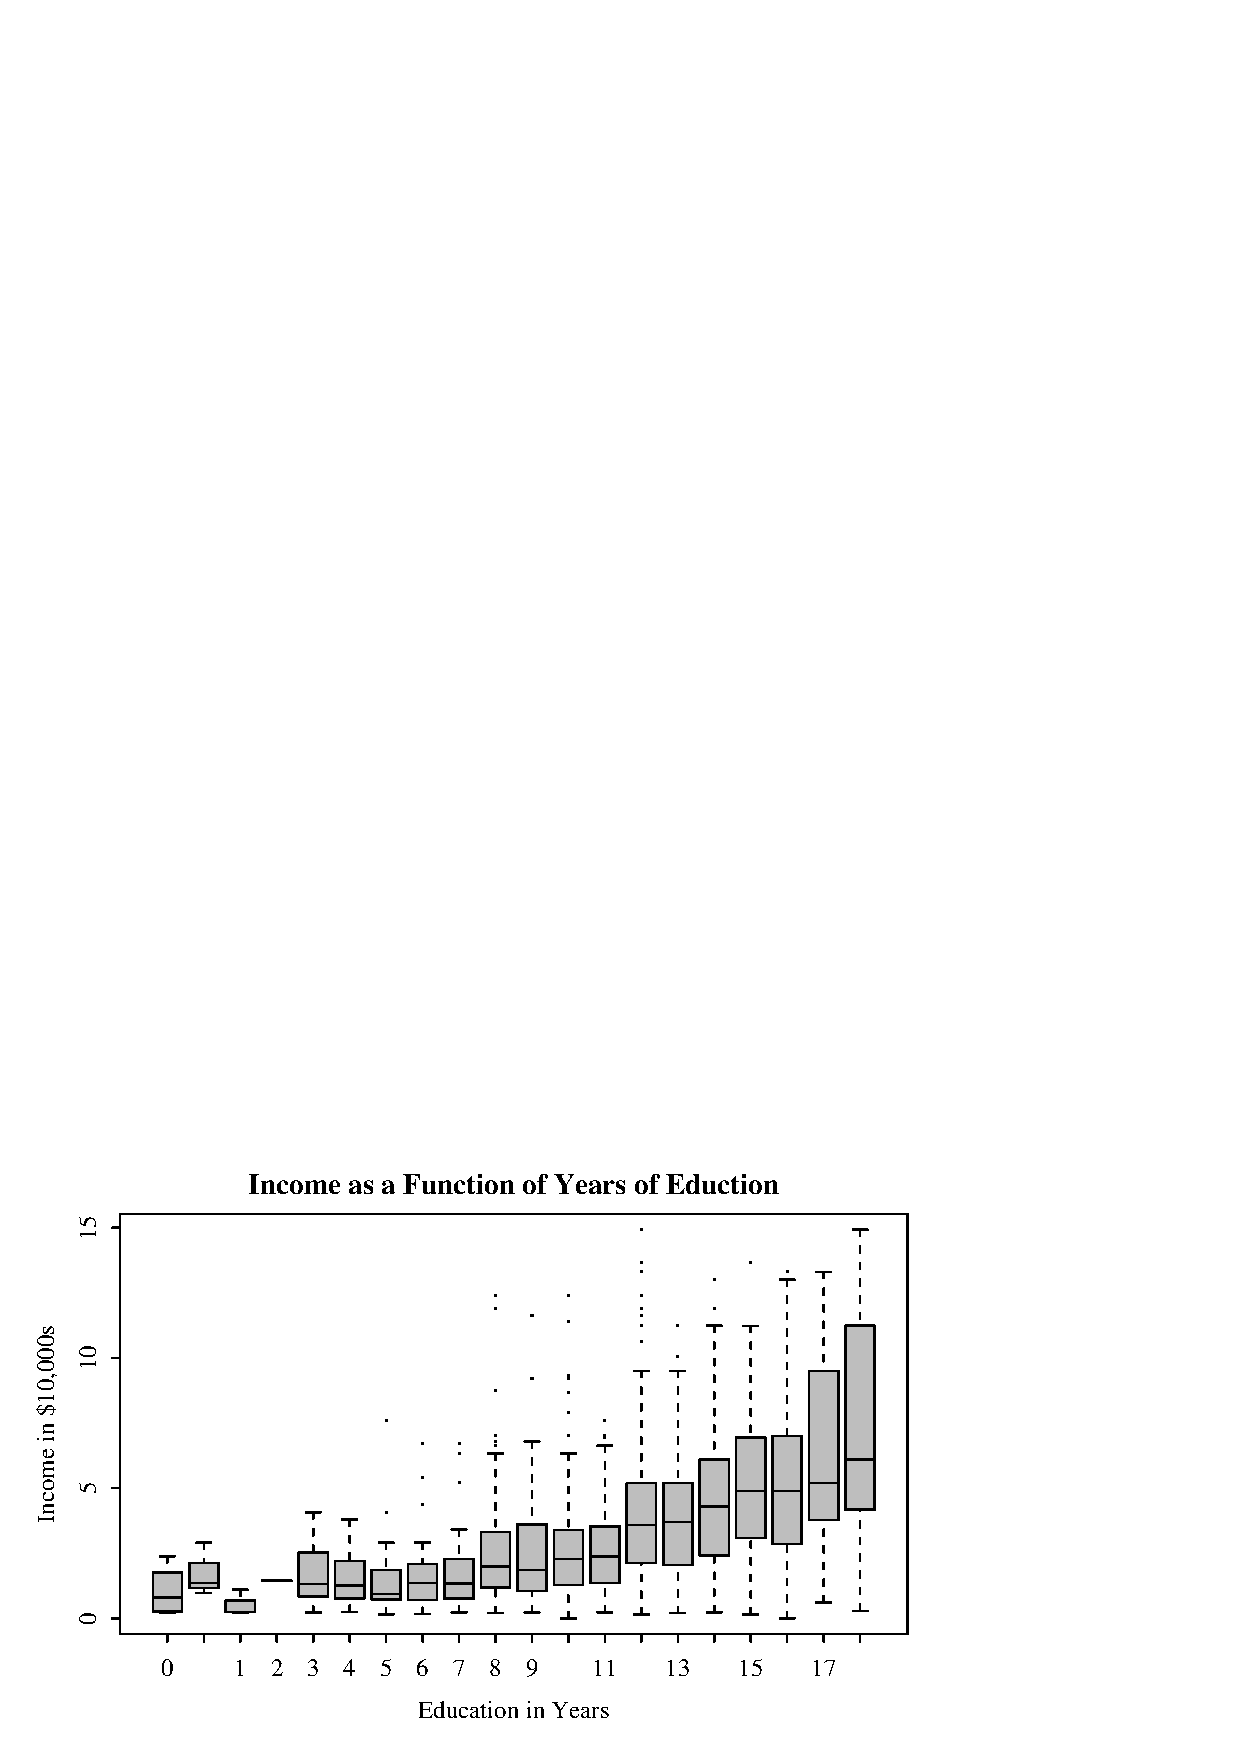
\includegraphics{figs/sample1}
\end{center}
Using the sample \texttt{turnout} data set included with Zelig, the
following commands will produce the graph above.
\begin{verbatim}
> library(Zelig)                             # Loads the Zelig package.
> data (turnout)                             # Loads the sample data.
> boxplot(income ~ educate,                  # Creates a boxplot with income
+  data = turnout, col = "grey", pch = ".",  #  as a function of education.  
+  main = "Income as a Function of Years of Education", 
+  xlab = "Education in Years", ylab = "Income in \$10,000s")
\end{verbatim}

\newpage

\subsection{Density Plots: A Histogram}

Histograms are easy ways to evaluate the density of a quantity of
interest.  

\begin{center}
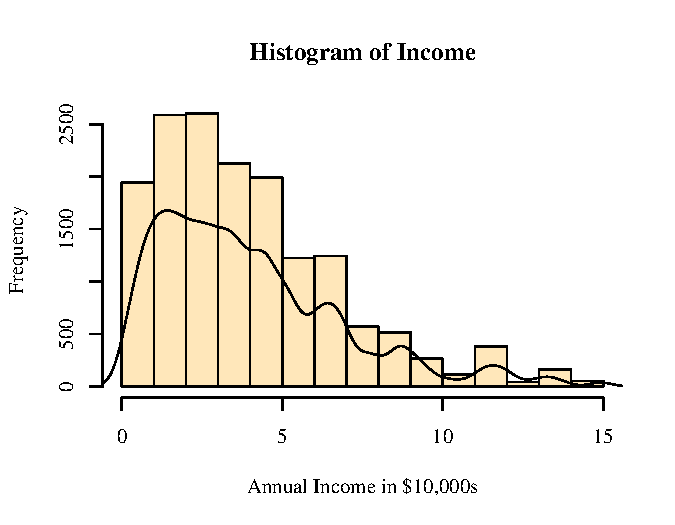
\includegraphics{figs/sample2}
\end{center}

Here's the code to create this graph:
\begin{verbatim}
> library(Zelig)                              # Loads the Zelig package.
> data(turnout)                               # Loads the sample data set.
> truehist(turnout$income,  col = "wheat1",   # Calls the main plot, with   
+      xlab = "Annual Income in $10,000s",    #  options.  
+      main = "Histogram of Income") 
> lines(density(turnout$income))              # Adds the kernel density line.  
\end{verbatim} %$

\newpage

\subsection{Advanced Examples} 

The examples above are simple examples which only skim the surface of
R's plotting potential.  We include more advanced, model-specific
plots in the Zelig demo scripts, and have created functions that
automate some of these plots, including:  

\begin{enumerate}
  
\item {\bf Ternary Diagrams} describe the predicted probability of a
  categorical dependent variable that has three observed outcomes.
  You may choose to use this plot with the multinomial logit, the
  ordinal logit, or the ordinal probit models (Katz and King,
  1999).\nocite{KatKin99} See \Sref{ternary} for the sample code, type
  {\tt demo(mlogit)} at the R prompt to run the example, and refer to
  Section \ref{ternary} to add points to a ternary diagram.
  
\begin{center}
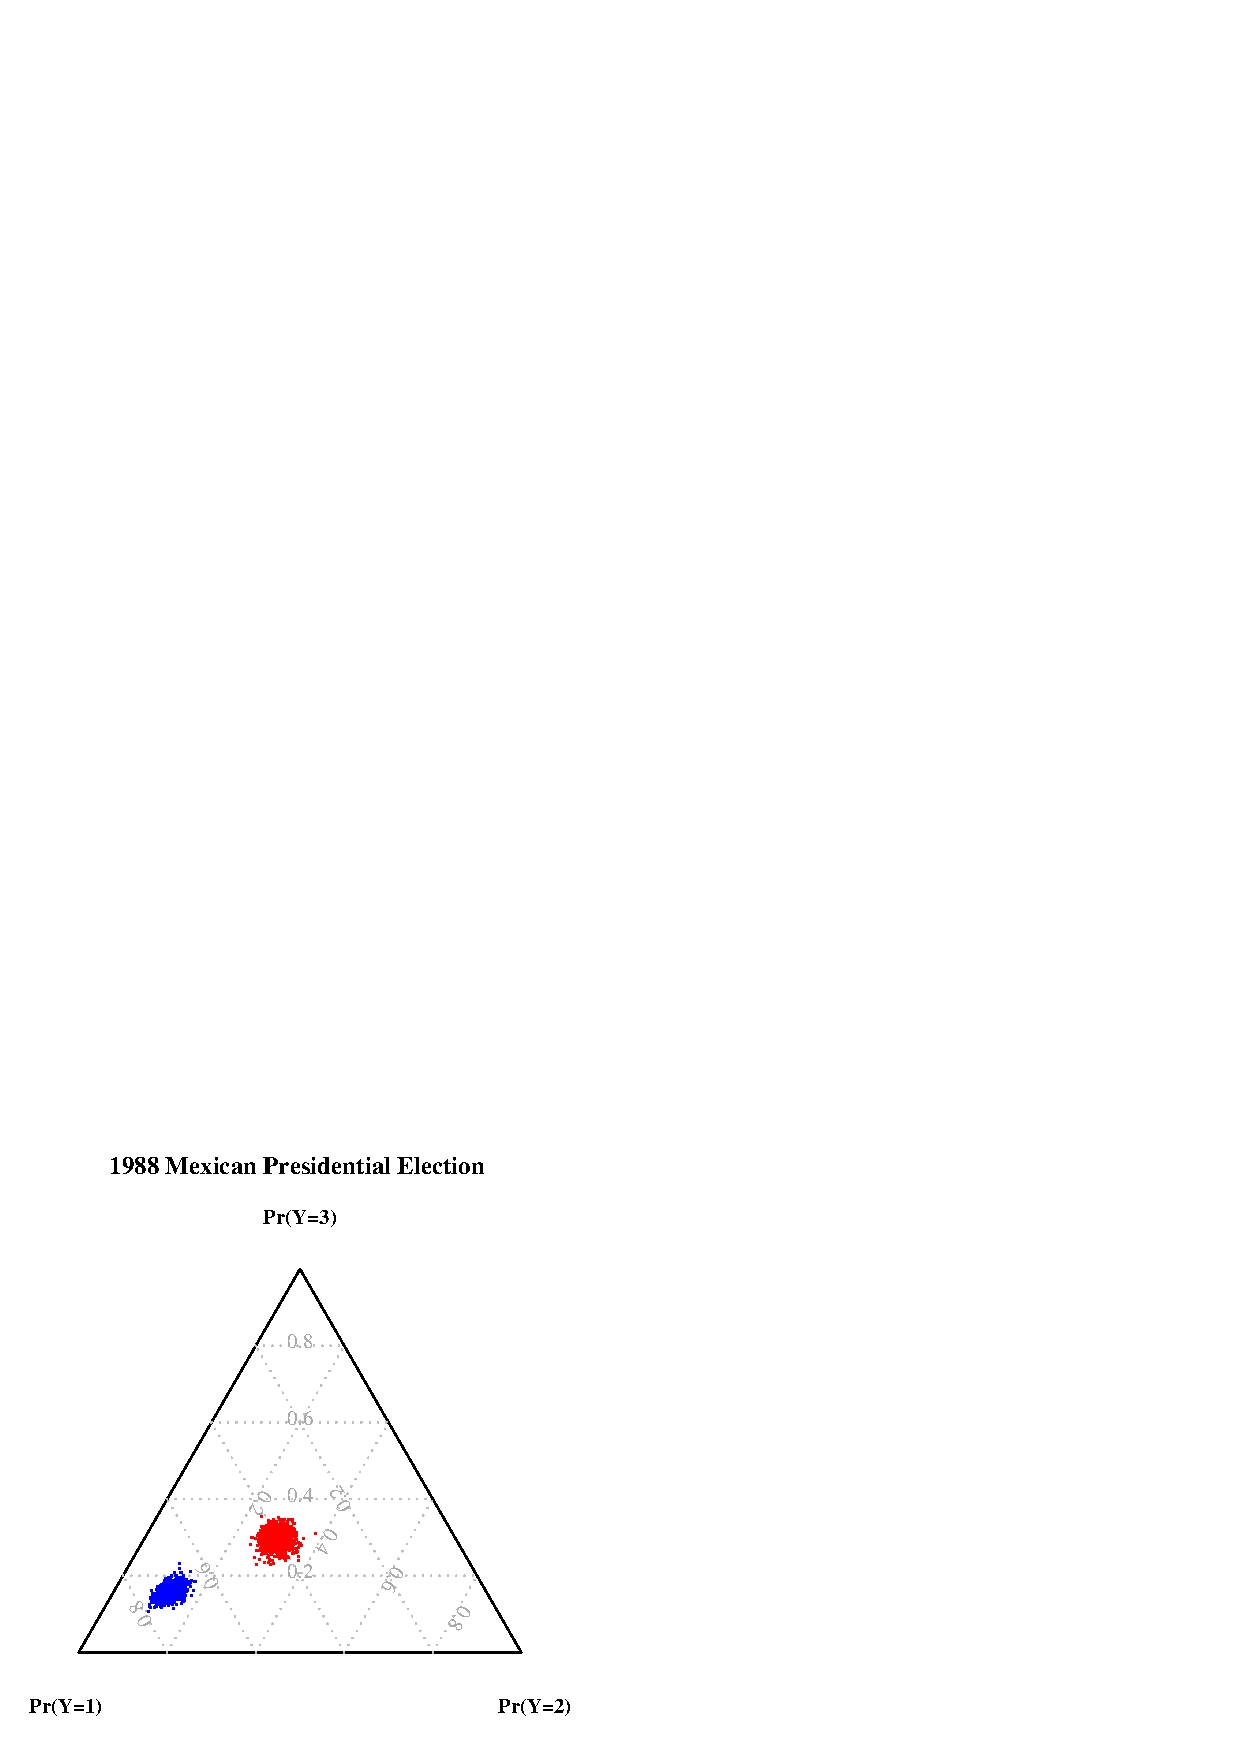
\includegraphics{figs/ternary}
\end{center}

\newpage

\item {\bf ROC Plots} summarize how well models for binary dependent
  variables (logit, probit, and relogit) fit the data.  The ROC plot
  evaluates the fraction of 0's and 1's correctly predicted for every
  possible threshold value at which the continuous Prob$(Y = 1)$ may
  be realized as a dichotomous prediction.  The closer the ROC curve
  is to the upper right corner of the plot, the better the fit of the
  model specification (King and Zeng, 2002\emph{b})\nocite{KinZen02}.
  See Section \ref{ROC} for the sample code, and type {\tt demo(roc)} at the
  R prompt to run the example.

\begin{center}
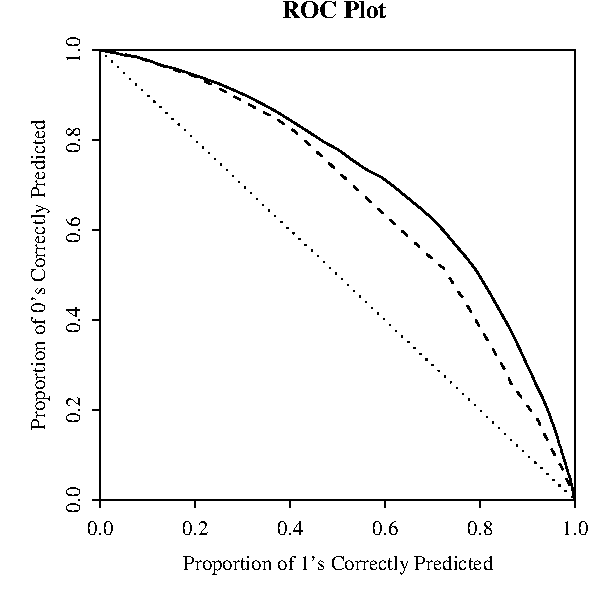
\includegraphics{figs/roc}
\end{center}

\newpage

\item {\bf Vertical Confidence Intervals} may be used for almost any
  model, and describe simulated confidence intervals for any quantity
  of interest while allowing one of the explanatory variables to vary
  over a given range of values (King, Tomz and Wittenberg,
  2000)\nocite{KinTomWit00}. Type {\tt demo(vertci)} at the R prompt to
  run the example, and {\tt help.zelig(plot.ci)} for the manual page.

\begin{center}
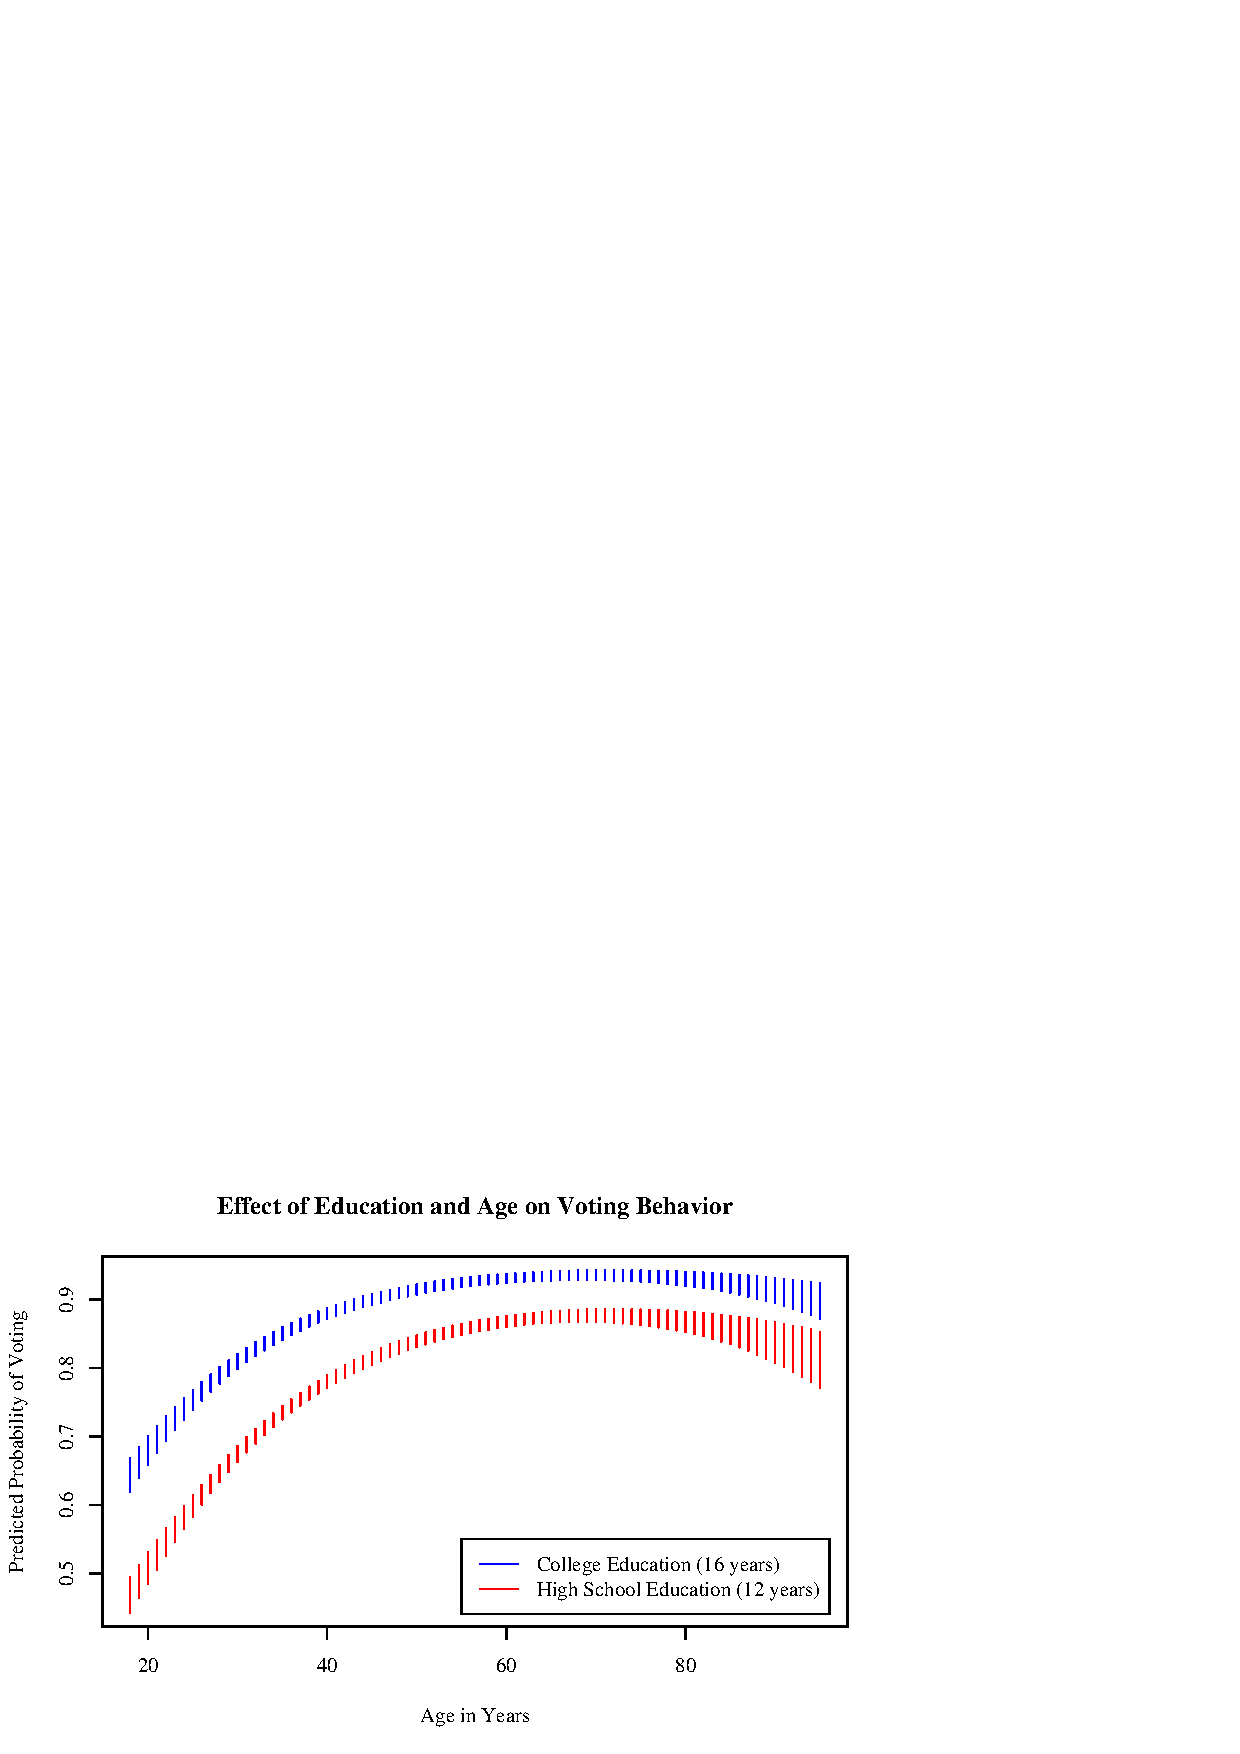
\includegraphics{figs/vertci}
\label{plot.vertci}
\end{center}

\end{enumerate}

%%% Local Variables: 
%%% mode: LaTeX
%%% TeX-master: "zelig"
%%% End:



\part{Advanced Zelig Uses}

\chapter{R Objects}\label{a:R}

In R, objects can have one or more classes, consisting of the class of
the scalar value and the class of the data structure holding the
scalar value.  Use the {\tt is()} command to determine what an object
\emph{is}.  If you are already familiar with R objects, you may skip
to \Sref{load.data} for loading data, or \Sref{s:commands} for a
description of Zelig commands.

\section{Scalar Values}\label{variables}

R uses several classes of scalar values, from which it constructs 
larger data structures.  R is highly class-dependent: certain
operations will only work on certain types of values or certain types
of data structures.  We list the three basic types of scalar values
here for your reference:  

\begin{enumerate}
\item \textbf{Numeric} is the default value type for most numbers.  An
  \texttt{integer} is a subset of the \texttt{numeric} class, and may
  be used as a \texttt{numeric} value.  You can perform
  any type of math or logical operation on numeric values,
  including:
\begin{verbatim}
> log(3 * 4 * (2 + pi))         # Note that pi is a built-in constant, 
   [1] 4.122270                 #   and log() the natural log function.
> 2 > 3                         # Basic logical operations, including >,
   [1] FALSE                    #   <, >= (greater than or equals), 
                                #   <= (less than or equals), == (exactly 
                                #   equals), and != (not equals). 
> 3 >= 2 && 100 == 1000/10      # Advanced logical operations, including
   [1] TRUE                     #   & (and), && (if and only if), | (or), 
                                #   and || (either or).
\end{verbatim}
  Note that \texttt{Inf} (infinity), \texttt{-Inf} (negative
  infinity), \texttt{NA} (missing value), and \texttt{NaN} (not a
  number) are special numeric values on which most math operations
  will fail.  (Logical operations will work, however.)

\item \textbf{Logical} operations create logical values of either
  \texttt{TRUE} or \texttt{FALSE}.  To convert logical values to
  numerical values, use the \texttt{as.integer()} command:
\begin{verbatim}
> as.integer(TRUE)
   [1] 1 
> as.integer(FALSE)
   [1] 0
\end{verbatim}
\item \textbf{Character} values are text strings.  For example, 
\begin{verbatim}
> text <- "supercalafragilisticxpaladocious"
> text
[1] "supercalafragilisticxpaladocious"
\end{verbatim}
  assigns the text string on the right-hand side of the \texttt{<-} to
  the named object in your workspace.  Text strings are primarily used
  with data frames, described in the next section.  R always returns
  character strings in quotes.
\end{enumerate}

\section{Data Structures}

\subsection{Arrays}

Arrays are data structures that consist of only one type of scalar
value (e.g., a vector of character strings, or a matrix of numeric
values).  The most common versions, one-dimensional and
two-dimensional arrays, are known as \emph{vectors} and
\emph{matrices}, respectively.  

\subsubsection*{Ways to create arrays}
\begin{enumerate}
\item Common ways to create {\bf vectors} (or one-dimensional arrays)
include:  
\begin{verbatim}
> a <- c(3, 7, 9, 11)    # Concatenates numeric values into a vector
> a <- c("a", "b", "c")  # Concatenates character strings into a vector
> a <- 1:5               # Creates a vector of integers from 1 to 5 inclusive  
> a <- rep(1, times = 5) # Creates a vector of 5 repeated `1's
\end{verbatim}
To manipulate a vector:  
\begin{verbatim}
> a[10]                # Extracts the 10th value from the vector `a'
> a[5] <- 3.14         # Inserts 3.14 as the 5th value in the vector `a'
> a[5:7] <- c(2, 4, 7) # Replaces the 5th through 7th values with 2, 4, and 7
\end{verbatim}
\emph{Unlike} larger arrays, vectors can be extended without first
creating another vector of the correct length.  Hence, 
\begin{verbatim}
> a <- c(4, 6, 8) 
> a[5] <- 9       # Inserts a 9 in the 5th position of the vector,
                  #  automatically inserting an `NA' values position 4 
\end{verbatim}

\item \label{factors} A {\bf factor vector} is a special type of
vector that allows users to create $j$ indicator variables in one
vector, rather than using $j$ dummy variables (as in Stata or SPSS).  R
creates this special class of vector from a pre-existing vector {\tt x}
using the {\tt factor()} command, which separates {\tt x} into levels
based on the discrete values observed in {\tt x}.  These values may be
either integer value or character strings.  For example,
\begin{verbatim}
> x <- c(1, 1, 1, 1, 1, 2, 2, 2, 2, 9, 9, 9, 9)
> factor(x)
   [1] 1 1 1 1 1 2 2 2 2 9 9 9 9
   Levels: 1 2 9
\end{verbatim}
By default, {\tt factor()} creates unordered factors, which are
  treated as discrete, rather than ordered, levels.  Add the optional
  argument {\tt ordered = TRUE} to order the factors in the vector:
\begin{verbatim}  
> x <- c("like", "dislike", "hate", "like", "don't know", "like", "dislike")
> factor(x, levels = c("hate", "dislike", "like", "don't know"),
+        ordered = TRUE)
  [1] like    dislike    hate    like   don't know   like   dislike   
Levels: hate < dislike < like < don't know
\end{verbatim}
  The {\tt factor()} command orders the levels according to the order in
  the optional argument {\tt levels}.  If you omit the levels command,
  R will order the values as they occur in the vector.  Thus, omitting
  the {\tt levels} argument sorts the levels as {\tt like < dislike <
    hate < don't know} in the example above.  If you omit one or more
  of the levels in the list of levels, R returns levels values of {\tt
    NA} for the missing level(s):
\begin{verbatim}
> factor(x, levels = c("hate", "dislike", "like"), ordered = TRUE)
  [1] like    dislike hate    like    <NA>    like    dislike
Levels: hate < dislike < like
\end{verbatim}
Use factored vectors within data frames for plotting (see
\Sref{ss:draw}), to set the values of the explanatory variables using
{\tt setx} (see \Sref{s:main}) and in the ordinal logit and multinomial
logit models (see \Sref{s:models}).  

\item Build {\bf matrices} (or two-dimensional arrays) from vectors
(one-dimensional arrays).  You can create a matrix in two ways:   
\begin{enumerate}
\item From a vector: Use the command \texttt{matrix(vector, nrow
    =} $k$\texttt{, ncol =} $n$\texttt{)} to create a $k \times n$
    matrix from the vector by filling in the columns from left to
    right.  For example,
\begin{verbatim}
> matrix(c(1,2,3,4,5,6), nrow = 2, ncol = 3)
        [,1] [,2] [,3]       # Note that when assigning a vector to a
   [1,]    1    3    5       #  matrix, none of the rows or columns 
   [2,]    2    4    6       #  have names.  
\end{verbatim}
\item From two or more vectors of length $k$: Use \texttt{cbind()} to
  combine $n$ vectors vertically to form a $k \times n$ matrix, 
  or \texttt{rbind()} to combine $n$ vectors horizontally to form a
  $n \times k$ matrix.  For example:
\begin{verbatim}
> x <- c(11, 12, 13)         # Creates a vector `x' of 3 values.
> y <- c(55, 33, 12)         # Creates another vector `y' of 3 values.  
> rbind(x, y)                # Creates a 2 x 3 matrix.  Note that row
     [,1] [,2] [,3]          #  1 is named x and row 2 is named y, 
   x   11   12   13          #  according to the order in which the
   y   55   33   12          #  arguments were passed to rbind().
> cbind(x, y)                # Creates a 3 x 2 matrix.  Note that the
         x  y                #  columns are named according to the
   [1,] 11 55                #  order in which they were passed to
   [2,] 12 33                #  cbind().  
   [3,] 13 12
\end{verbatim}
\end{enumerate}
R supports a variety of matrix functions, including: \texttt{det()},
which returns the matrix's determinant; \texttt{t()}, which transposes
the matrix; \texttt{solve()}, which inverts the the matrix; and
\texttt{\%*\%}, which multiplies two matricies.  In addition, the
\texttt{dim()} command returns the dimensions of your matrix.  As with
vectors, square brackets extract specific values from a matrix and the
assignment mechanism \texttt{<-} replaces values.  For example:
\begin{verbatim}
> loo[,3]     		  # Extracts the third column of loo.  
> loo[1,]      		  # Extracts the first row of loo.  
> loo[1,3] <- 13          # Inserts 13 as the value for row 1, column 3.  
> loo[1,] <- c(2,2,3)     # Replaces the first row of loo.  
\end{verbatim}
If you encounter problems replacing rows or columns, make sure that
the \texttt{dims()} of the vector matches the \texttt{dims()} of the
matrix you are trying to replace.  

\item An \textbf{n-dimensional array} is a set of stacked matrices of identical
  dimensions.  For example, you may create a three dimensional array
  with dimensions $(x, y, z)$ by stacking $z$ matrices each with $x$
  rows and $y$ columns.  
\begin{verbatim}
> a <- matrix(8, 2, 3)       # Creates a 2 x 3 matrix populated with 8's.
> b <- matrix(9, 2, 3)       # Creates a 2 x 3 matrix populated with 9's.
> array(c(a, b), c(2, 3, 2)) # Creates a 2 x 3 x 2 array with the first
   , , 1                     #  level [,,1] populated with matrix a (8's),
                             #  and the second level [,,2] populated 
        [,1] [,2] [,3]       #  with matrix b (9's).  
   [1,]    8    8    8       
   [2,]    8    8    8       # Use square brackets to extract values.  For
                             #  example, [1, 2, 2] extracts the second
   , , 2                     #  value in the first row of the second level.
                             # You may also use the <- operator to 
        [,1] [,2] [,3]       #  replace values.  
   [1,]    9    9    9
   [2,]    9    9    9
\end{verbatim}
If an array is a one-dimensional vector or two-dimensional matrix, R
  will treat the array using the more specific method.  
\end{enumerate}

Three functions especially helpful for
arrays:  
\begin{itemize}
\item {\tt is()} returns both the type of scalar value that populates
the array, as well as the specific type of array (vector, matrix, or
array more generally).
\item {\tt dims()} returns the size of an array, where 
\begin{verbatim}
> dims(b) 
 [1]  33  5
\end{verbatim} 
indicates that the array is two-dimensional (a matrix), and has 33
rows and 5 columns.  
\item The single bracket \verb|[ ]| indicates specific values in the
array.  Use commas to indicate the index of the specific values you
would like to pull out or replace:  
\begin{verbatim}
> dims(a)
 [1]  14
> a[10]       # Pull out the 10th value in the vector `a'
> dims(b) 
 [1]  33  5
> b[1:12, ]   # Pull out the first 12 rows of `b' 
> c[1, 2]     # Pull out the value in the first row, second column of `c'
> dims(d)
 [1]  1000  4  5
> d[ , 3, 1]  # Pulls out a vector of 1,000 values 
\end{verbatim}
\end{itemize} 

\subsection{Lists}

Unlike arrays, which contain only one type of scalar value, lists
are flexible data structures that can contain heterogeneous value types
and heterogeneous data structures.  Lists are so flexible that one list
can contain another list.  For example, the list {\tt output} can
contain {\tt coef}, a vector of regression coefficients; {\tt
variance}, the variance-covariance matrix; and another list {\tt terms}
that describes the data using character strings.  Use the {\tt
names()} function to view the named elements in a list, and to extract
a named element, use
\begin{verbatim}
> names(output)
 [1] coefficients   variance   terms
> output$coefficients
\end{verbatim} %$
For lists where the elements are not named, use double square brackets
\verb|[[ ]]| to extract elements:  
\begin{verbatim}
> L[[4]]      # Extracts the 4th element from the list `L'
> L[[4]] <- b # Replaces the 4th element of the list `L' with a matrix `b'
\end{verbatim}

Like vectors, lists are flexible data structures that can be extended
without first creating another list of with the correct number of
elements:  
\begin{verbatim}
> L <- list()                      # Creates an empty list
> L$coefficients <- c(1, 4, 6, 8)  # Inserts a vector into the list, and 
                                   #  names that vector `coefficients' 
				   #  within the list
> L[[4]] <- c(1, 4, 6, 8)          # Inserts the vector into the 4th position
                                   #  in the list.  If this list doesn't 
                                   #  already have 4 elements, the empty 
                                   #  elements will be `NULL' values
\end{verbatim} %$
Alternatively, you can easily create a list using objects that already
exist in your workspace:  
\begin{verbatim}
> L <- list(coefficients = k, variance = v) # Where `k' is a vector and
                                            #   `v' is a matrix
\end{verbatim}

\subsection{Data Frames}

A data frame (or data set) is a special type of list in which each
variable is constrained to have the same number of observations.  A
data frame may contain variables of different types (numeric,
integer, logical, character, and factor), so long as each variable has
the same number of observations. 

Thus, a data frame can use both matrix commands and list commands to
manipulate variables and observations.  
\begin{verbatim}
> dat[1:10,]         # Extracts observations 1-10 and all associated variables  
> dat[dat$grp == 1,] # Extracts all observations that belong to group 1 
> group <- dat$grp   # Saves the variable `grp' as a vector `group' in
                     #   the workspace, not in the data frame
> var4 <- dat[[4]]   # Saves the 4th variable as a `var4' in the workspace
\end{verbatim} 

For a comprehensive introduction to data frames and recoding data, see
\Sref{load.data}.

\subsection{Identifying Objects and Data Structures}

Each data structure has several \emph{attributes} which describe it.
Although these attributes are normally invisible to users (e.g., not
printed to the screen when one types the name of the object), there are
several helpful functions that display particular attributes:  
\begin{itemize}
\item For arrays, {\tt dims()} returns the size of each dimension.  
\item For arrays, {\tt is()} returns the scalar value type and
specific type of array (vector, matrix, array).  For more complex data
structures, {\tt is()} returns the default methods (classes) for that object. 
\item For lists and data frames, {\tt names()} returns the variable
names, and {\tt str()} returns the variable names and a short
description of each element.  
\end{itemize}  
For almost all data types, you may use {\tt summary()} to get summary
statistics.  

\chapter{Programming Statements}

This chapter introduces the main programming commands.  These include
functions, if-else statements, for-loops, and special procedures for
managing the inputs to statistical models.  

\section{Functions}

Functions are either built-in or user-defined sets of encapsulated
commands which may take any number of arguments.  Preface a function
with the {\tt function} statement and use the {\tt <-}
operator to assign functions to objects in your workspace.  

You may use functions to run the same procedure on different objects
in your workspace.  For example, 
\begin{verbatim}
check <- function(p, q) { 
 result <- (p - q)/q
 result
 }
\end{verbatim}
is a simple function with arguments {\tt p} and {\tt q} which
calculates the difference between the $i$th elements of the vector
{\tt p} and the $i$th element of the vector {\tt q} as a proportion of
the $i$th element of {\tt q}, and returns the resulting vector.  For
example, {\tt check(p = 10, q = 2)} returns 4.  You may omit the
descriptors as long as you keep the arguments in the correct order:
{\tt check(10, 2)} also returns 4.  You may also use other objects as
inputs to the function.  If {\tt again = 10} and {\tt really = 2},
then {\tt check(p = again, q = really)} and {\tt check(again, really)}
also returns 4.

Because functions run commands as a set, you should make sure that
each command in your function works by testing each line of the
function at the R prompt.

\section{If-Statements}

Use {\tt if} (and optionally, {\tt else}) to control the flow of R
functions.  For example, let {\tt x} and {\tt y} be scalar numerical
values:  
\begin{verbatim}
if (x == y) {                # If the logical statement in the ()'s is true,  
  x <- NA                    #  then `x' is changed to `NA' (missing value). 
}
else {                       # The `else' statement tells R what to do if  
  x <- x^2                   #  the if-statement is false.  
} 
\end{verbatim}
As with a function, use {\tt \{} and {\tt \}} to define the set of commands associated
with each if and else statement.  (If you include if
statements inside functions, you may have multiple sets of nested
curly braces.)

\section{For-Loops}

Use {\tt for} to repeat (loop) operations.  Avoiding loops by using matrix
or vector commands is usually faster and more elegant, but loops are
sometimes necessary to assign values.  If you are using a loop to
assign values to a data structure, you must first initialize an empty
data structure to hold the values you are assigning.

Select a data structure compatible with the type of output your loop
will generate.  If your loop generates a scalar, store it in a vector
(with the $i$th value in the vector corresponding to the the $i$th run
of the loop).  If your loop generates vector output, store them as
rows (or columns) in a matrix, where the $i$th row (or column)
corresponds to the $i$th iteration of the loop.  If your output
consists of matrices, stack them into an array.  For list output (such
as regression output) or output that changes dimensions in each
iteration, use a list.  To initialize these data structures, use:
\begin{verbatim}
> x <- vector()                          # An empty vector of any length.
> x <- list()                            # An empty list of any length.  
\end{verbatim}
The {\tt vector()} and {\tt list()} commands create a vector or list
of any length, such that assigning {\tt x[5] <- 15} automatically
creates a vector with 5 elements, the first four of which are empty
values ({\tt NA}).  In contrast, the {\tt matrix()} and {\tt array()}
commands create data structures that are restricted to their original
dimensions.  
\begin{verbatim}
> x <- matrix(nrow = 5, ncol = 2)  # A matrix with 5 rows and 2 columns.
> x <- array(dim = c(5,2,3))       # A 3D array of 3 stacked 5 by 2 matrices.
\end{verbatim}
If you attempt to assign a value at $(100, 200, 20)$ to either of
these data structures, R will return an error message (``subscript is
out of bounds'').  R does not automatically extend the
dimensions of either a matrix or an array to accommodate additional
values.  

\paragraph{Example 1: Creating a vector with a logical statement} 
\begin{verbatim}
x <- array()             # Initializes an empty data structure.  
for (i in 1:10) {        # Loops through every value from 1 to 10, replacing
  if (is.integer(i/2)) { #  the even values in `x' with i+5.
    x[i] <- i + 5 
  }      
}                        # Enclose multiple commands in {}.  
\end{verbatim}
You may use {\tt for()} inside or outside of functions.  

\paragraph{Example 2: Creating dummy variables by hand}  

\label{dummy}You may also use a loop to create a matrix of dummy
variables to append to a data frame.  For example, to generate fixed
effects for each state, let's say that you have {\tt mydata} which
contains {\tt y}, {\tt x1}, {\tt x2}, {\tt x3}, and {\tt state}, with
{\tt state} a character variable with 50 unique values.  There are
three ways to create dummy variables: 1) with a built-in R command; 2)
with one loop; or 3) with 2 for loops.  
\begin{enumerate}
\item R will create dummy variables on the fly from a single variable
with distinct values.  
\begin{verbatim}
> z.out <- zelig(y ~ x1 + x2 + x3 + as.factor(state), 
                 data = mydata, model = "ls")
\end{verbatim}
This method returns $k - 1$ indicators for $k$ states.  

\item Alternatively, you can use a loop to create dummy variables by
hand.  There are two ways to do this, but both start with the same
initial commands. Using vector commands, first create an index of for
the states, and initialize a matrix to hold the dummy variables:
\begin{verbatim}  
idx <- sort(unique(mydata$state))
dummy <- matrix(NA, nrow = nrow(mydata), ncol = length(idx))
\end{verbatim}  %$
Now choose between the two methods.  
\begin{enumerate}
\item The first method is computationally inefficient, but more intuitive for users not
accustomed to vector operations.  The first loop uses {\tt i} as in
index to loop through all the rows, and the second loop uses {\tt j}
to loop through all 50 values in the vector {\tt idx}, which
correspond to columns 1 through 50 in the matrix {\tt dummy}.
\begin{verbatim}
for (i in 1:nrow(mydata)) {
  for (j in 1:length(idx)) {
    if (mydata$state[i,j] == idx[j]) {
      dummy[i,j] <- 1
    }
    else {
      dummy[i,j] <- 0
    }
  }
}
\end{verbatim}  % $
Then add the new matrix of dummy variables to your data frame:
\begin{verbatim}
names(dummy) <- idx
mydata <- cbind(mydata, dummy) 
\end{verbatim}  

\item As you become more comfortable with vector operations, you can
replace the double loop procedure above with one loop:   
\begin{verbatim}
for (j in 1:length(idx)) { 
  dummy[,j] <- as.integer(mydata$state == idx[j])
}
\end{verbatim} %$
The single loop procedure evaluates each element in {\tt idx} against the vector {\tt mydata\$state}.  This creates a vector of $n$ {\tt
    TRUE}/{\tt FALSE} observations, which you may transform to {\tt
    1}'s and {\tt 0}'s using {\tt as.integer()}.  Assign the resulting
  vector to the appropriate column in {\tt dummy}.  Combine the {\tt
dummy} matrix with the data frame as above to complete the procedure.
\end{enumerate}
\end{enumerate}

\paragraph{Example 3: Weighted regression with subsets}  

Selecting the {\tt by} option in {\tt zelig()} partitions the data
frame and then automatically loops the specified model through each
partition.  Suppose that {\tt mydata} is a data frame with variables
{\tt y}, {\tt x1}, {\tt x2}, {\tt x3}, and {\tt state}, with {\tt
state} a factor variable with 50 unique values.  Let's say that you
would like to run a weighted regression where each observation is
weighted by the inverse of the standard error on {\tt x1}, estimated
for that observation's state.  In other words, we need 
to first estimate the model for each of the 50 states, calculate 1 /
{\sc se}({\tt x1}$_j$) for each state $j = 1, \dots, 50$, and then
assign these weights to each observation in {\tt mydata}.    
\begin{itemize}
\item Estimate the model separate for each state using the {\tt by}
option in {\tt zelig()}:  
\begin{verbatim}
z.out <- zelig(y ~ x1 + x2 + x3, by = "state", data = mydata, model = "ls")
\end{verbatim}
Now {\tt z.out} is a list of 50 regression outputs.  
\item Extract the standard error on {\tt x1} for each of the state
level regressions.  
\begin{verbatim}
se <- array()                          # Initalize the empty data structure.
for (i in 1:50) {                      # vcov() creates the variance matrix
  se[i] <- sqrt(vcov(z.out[[i]])[2,2]) # Since we have an intercept, the 2nd 
}                                      # diagonal value corresponds to x1.
\end{verbatim}
\item Create the vector of weights.  
\begin{verbatim}
wts <- 1 / se
\end{verbatim}
This vector {\tt wts} has 50 values that correspond to the 50 sets of
state-level regression output in {\tt z.out}.  
\item To assign the vector of weights to each observation, we need to
match each observation's state designation to the appropriate state.
For simplicity, assume that the states are numbered 1 through 50.
\begin{verbatim}
mydata$w <- NA            # Initalizing the empty variable
for (i in 1:50) { 
  mydata$w[mydata$state == i] <- wts[i]
} 
\end{verbatim} %$
We use {\tt mydata\$state} as the index (inside the square brackets)
to assign values to {\tt mydata\$w}.  Thus, whenever state equals 5
for an observation, the loop assigns the fifth value in the vector
{\tt wts} to the variable {\tt w} in {\tt mydata}.  If we had 500
observations in {\tt mydata}, we could use this method to match each
of the 500 observations to the appropriate {\tt wts}.

If the states are character strings instead of integers, we can use a
slightly more complex version
\begin{verbatim}
mydata$w <- NA
idx <- sort(unique(mydata$state))
for (i in 1:length(idx) { 
  mydata$w[mydata$state == idx[i]] <- wts[i]
}
\end{verbatim}   

\item Now we can run our weighted regression:  
\begin{verbatim}
z.wtd <- zelig(y ~ x1 + x2 + x3, weights = w, data = mydata, 
               model = "ls")
\end{verbatim}

\end{itemize}  



%%% Local Variables: 
%%% mode: latex
%%% TeX-master: "zelig"
%%% End: 

\chapter{Writing New Models} \label{s:new}

With Zelig, writing a new model in R is straightforward.  (If you
already have a model, see Chapter \ref{c:addingmodels} for how to include it in
Zelig.)  With tools to streamline user inputs, writing a new model
does not require a lot of programming knowledge, but lets developers
focus on the model's math.  Generally, writing a new statistical
procedure or model comes in orderly steps:  
\begin{enumerate}
\item Write down the mathematical model. Define the parameters that
you need, grouping parameters into convenient vectors or matrices
whenever possible (this will make your code clearer).  
\item Write the code.  
\item Test the code (usually using Monte Carlo data, where you know
the true values being estimated ) and make sure
that it works as expected. 
\item Write some documentation explaining your model and the functions
that run your model.  
\end{enumerate}
Somewhere between steps [1] and [2], you will need to translate input
data into the mathematical notation that you used to write down the
model.  Rather than repeating whole blocks of code, use functions to
streamline the number of commands that users will need to run your
model.  

With more steps being performed by fewer commands, the inputs to these
commands become more sophisticated.  The structure of those inputs
actually matters quite a lot.  If your function has a convoluted
syntax, it will be difficult to use, difficult to explain, and
difficult to document.  If your function is easy to use and has an
intuitive syntax, however, it will be easy to explain and document,
which will make your procedure more accessible to all users.

\section{Managing Statistical Model Inputs}
\label{ui}  

Most statistical models require a matrix of explanatory variables and
a matrix of dependent variables.  Rather than have users create
matrices themselves, R has a convenient user interface to create
matrices of response and explanatory variables on the fly.  Users
simply specify a {\tt formula} in the form of 
\verb|dependent ~ explanatory variables|, and developers use the
following functions to transform the formula into the appropriate
matrices.  Let {\tt mydata} be a data frame.  
\begin{verbatim}
> formula <- y ~ x1 + x2                   # User input

# Given the formula above, programmers can use the following standard commands
> D <- model.frame(formula, data = mydata) # Subset & listwise deletion
> X <- model.matrix(formula, data = D)     # Creates X matrix
> Y <- model.response(D)                   # Creates Y matrix
\end{verbatim}
where 
\begin{itemize}
\item {\tt D} is a subset of {\tt mydata} that contains only the
variables specified in the formula ({\tt y}, {\tt x1}, and {\tt x2})
with listwise deletion performed on the subset data frame; 
\item {\tt X} is a matrix that contains a column of 1's, and the
explanatory variables {\tt x1} and {\tt x2} from {\tt D}; and
\item {\tt Y} is a matrix containing the dependent variable(s) from
{\tt D}.  
\end{itemize}  
Depending on the model, {\tt Y} may be a column vector, matrix, or
other data structure.  

\subsection{Describe the Statistical Model}  

After setting up the $X$ matrix, the next step for most models will be
to identify the corresponding vector of parameters.  For a single
response variable model with no ancillary parameters, the standard R
interface is quite convenient: given $X$, the model's parameters are
simply $\beta$.

There are very few models, however, that fall into this category.
Even Normal regression, for example, has two sets of parameters
$\beta$ and $\sigma^2$.  In order to make the R formula format more
flexible, Zelig has an additional set of tools that lets you describe
the inputs to your model (for multiple sets of parameters).

After you have written down the statistical model, identify the
parameters in your model.  With these parameters in mind, the first
step is to write a {\tt describe.*()} function for your model.  If
your model is called {\tt mymodel}, then the {\tt describe.mymodel()}
function takes no arguments and returns a list with the following
information:
\begin{itemize}
\item {\tt category}: a character string that describes the dependent
variable.  See \Sref{categories} for the current list of available
categories.  
\item {\tt parameters}:  a list containing parameter sets used in your
model.  For each parameter (e.g., theta), you need to provide the
following information:  

\begin{itemize}

\item {\tt equations}: an integer number of equations for the
parameter.  For parameters that can take, for example, two to four
equations, use {\tt c(2, 4)}.  

\item {\tt tagsAllowed}: a logical value ({\tt TRUE}/{\tt FALSE})
specifying whether a given parameter allows constraints.  

\item {\tt depVar}: a logical value ({\tt TRUE}/{\tt FALSE})
specifying whether a parameter requires a corresponding dependent
variable.  

\item {\tt expVar}: a logical value ({\tt TRUE}/{\tt FALSE})
specifying whether a parameter allows explanatory variables.  

\end{itemize}
\end{itemize}
(See \Sref{describe.mymodel} for examples and additional arguments
output by {\tt describe.mymodel()}.)

\subsection{Single Response Variable Models: Normal Regression Model}
\label{normal.regression}

Let's say that you are trying to write a Normal regression model with
stochastic component
\begin{displaymath}
\textrm{Normal}(y_i \mid \mu_i, \sigma^2) \; = \; \frac{1}{\sqrt{2 \pi} \sigma} \, \exp
\left( -\left( \frac{(y_i - \mu_i)^2}{2 \sigma^2} \right) \right)
\end{displaymath}
with scalar variance parameter $\sigma^2 > 0$, and systematic component
$E(Y_i) = \mu_i = x_i \beta$.  This implies two sets of parameters in your
model, and the following {\tt describe.normal.regression()} function:
\begin{verbatim}
describe.normal.regression <- function() {
  category <- "continuous"
  mu <- list(equations = 1,              # Systematic component
             tagsAllowed = FALSE,
             depVar = TRUE,
             expVar = TRUE)
  sigma2 <- list(equations = 1,          # Scalar ancillary parameter
                 tagsAllowed = FALSE,
                 depVar = FALSE,
                 expVar = FALSE)
  pars <- list(mu = mu, sigma2 = sigma2)
  list(category = category, parameters = pars)
}
\end{verbatim}

To find the log-likelihood:  
\begin{eqnarray*}
\textrm{L }(\beta, \sigma^2 \mid y) & = & \prod_{1=1}^n
       \textrm{Normal}(y_i \mid \mu_i, \sigma^2)\\
    & = & \prod_{i=1}^n (2\pi\sigma^2)^{-1/2}\exp\left(\frac{-(y_i-\mu_i)^2}
{2\sigma^2}\right)\\
    & = &(2\pi\sigma^2)^{-n/2} \prod_{i=1}^n \exp\left(\frac{-(y_i-\mu_i)^2}
{2\sigma^2}\right)\\
    & = &(2\pi\sigma^2)^{-n/2} \prod_{i=1}^n \exp\left(\frac{-(y_i-x_i \beta)^2}
{2\sigma^2}\right)\\
\ln \textrm{L }(\beta, \sigma^2 \mid y) &=& -\frac{n}{2}\ln(2\pi\sigma^2)-
\sum_{i=1}^n \frac{(y_i-x_i\beta)^2}{2\sigma^2}\\
       &=& -\frac{n}{2}\ln(2\pi\sigma^2)-
        \frac{1}{2\sigma^2}\sum_{i=1}^n (y_i-x_i\beta)^2 \\
&\propto& -\frac{1}{2} \left( n \ln\sigma^2 + \frac{\sum_{i=1}^n
(y_i-x_i\beta)^2}{\sigma^2} \right)
\end{eqnarray*}
In R code, this translates to:  
\begin{verbatim}
ll.normal <- function(par, X, Y, n, terms) {
  beta <- parse.par(par, terms, eqn = "mu")             # [1]
  gamma <- parse.par(par, terms, eqn = "sigma2")        # [2]
  sigma2 <- exp(gamma)
  -0.5 * (n * log(sigma2) + sum((Y - X %*% beta)^2 / sigma2))
}
\end{verbatim}
At Comment [1] above, we use the function {\tt parse.par()}
to pull out the vector of parameters {\tt beta} (which relate the
systematic component $\mu_i$ to the explanatory variables $x_i$).  No
matter how many covariates there are, the {\tt parse.par()} function
can use {\tt terms} to pull out the appropriate parameters from {\tt par}.
We also use {\tt parse.par()} at Comment [2] to pull out the scalar
ancillary parameter that (after transformation) corresponds to the
$\sigma^2$ parameter. 

To optimize this function, simply type:  
\begin{verbatim}
out <- optim(start.val, ll.normal, control = list(fnscale = -1),
             method = "BFGS", hessian = TRUE, X = X, Y = Y, terms = terms)
\end{verbatim}
where
\begin{itemize}
\item {\tt start.val} is a vector of starting values for {\tt par}.
Use {\tt set.start()} to create starting values for all parameters,
systematic and ancillary, in one step.  
\item {\tt ll.normal} is the log-likelihood function derived above.
\item {\tt "BFGS"} specifies unconstrained optimization using a
  quasi-Newton method.
\item {\tt control = list(fnscale = -1)} specifies that R should
  maximize the function (omitting this causes R to minimize the
  function by default).
\item {\tt hessian = TRUE} instructs R to return the Hessian matrix
  (from which you may calculate the variance-covariance matrix).
\item {\tt X} and {\tt Y} are the matrix of explanatory variables and
  vector of dependent variables, used in the {\tt ll.normal()}
  function.
\item {\tt terms} are meta-data constructed from the {\tt
model.frame()} command.  
\end{itemize}
Please refer to the R-help for {\tt optim()} for more options.

To make this procedure generalizable, we can write a function that
takes a user-specified data frame and formula, and optional starting
values for the optimization procedure:  
\begin{verbatim}
normal.regression <- function(formula, data, start.val = NULL, ...) {

  fml <- parse.formula(formula, model = "normal.regression") # [1]
  D <- model.frame(fml, data = data)
  X <- model.matrix(fml, data = D)
  Y <- model.response(D)
  terms <- attr(D, "terms")
  n <- nrow(X)

  start.val <- set.start(start.val, terms)

  res <- optim(start.val, ll.normal, method = "BFGS",        
               hessian = TRUE, control = list(fnscale = -1),
               X = X, Y = Y, n = n, terms = terms, ...)      # [2]

  fit <- model.end(res, D)                                   # [3]
  fit$n <- n
  class(fit) <- "normal"                                     # [4]
  fit                                                        
}
\end{verbatim} %$
The following comments correspond to the bracketed numbers above:  
\begin{enumerate}
\item The {\tt parse.formula()} command looks for the {\tt
describe.normal.regression()} function, which changes the
user-specified formula into the following format:  
\begin{verbatim}
list(mu = formula,         # where `formula' was specified by the user
     sigma = ~ 1)
\end{verbatim}
\item The {\tt \dots} here indicate that if the user enters any
additional arguments when calling {\tt normal.regression()}, that
those arguments should go to the {\tt optim()} function.  
\item The {\tt model.end()} function takes the optimized output and
the listwise deleted data frame {\tt D} and creates an object that
will work with {\tt setx()}.  
\item Choose a class for your model output so that you will be able to
write an appropriate {\tt summary()}, {\tt param()}, and {\tt qi()}
function for your model.  
\end{enumerate}

\subsection{Multivariate models: Bivariate Normal example}\label{bivariate.probit}

Most common models have one systematic component.  For $n$
observations, the systematic component varies over observations $i = 1,
\dots, n$.  In the case of the Normal regression model, the systematic
component is $\mu_i$ ($\sigma^2$ is not estimated as a function of
covariates).

In some cases, however, your model may have more than one systematic
component.  In the case of bivariate probit, we have a dependent
variable $Y_i = (Y_{i1}, Y_{i2})$ observed as (0,0), (1,0), (0,1), or
(1,1) for $i = 1, \dots, n$.  Similar to a single-response probit model,
the stochastic component is described by two latent (unobserved)
continuous variables ($Y_{i1}^*$, $Y_{i2}^*$) which follow the
bivariate Normal distribution:
\begin{eqnarray*}
  \left ( \begin{array}{c} 
      Y_{i1}^* \\
      Y_{i2}^* 
    \end{array}
  \right ) &\sim &  
  \textrm{Normal} \left \{ \left ( 
      \begin{array}{c}
        \mu_{i1} \\ \mu_{i2}
      \end{array} \right ), \left( \begin{array}{cc}
                 1 & \rho \\
                 \rho & 1 
                 \end{array} \right) \right\},
\end{eqnarray*}
where for $j = 1, 2$, $\mu_{ij}$ is the mean for $Y_{ij}^*$ and $\rho$ is a
correlation parameter. The following observation mechanism links the
observed dependent variables, $Y_{ij}$, with these latent variables
\begin{eqnarray*}
Y_{ij} & = & \left \{ \begin{array}{cc}
                   1 & {\rm if} \; Y_{ij}^* \ge 0, \\
                   0 & {\rm otherwise.}
                   \end{array} 
                   \right.
\end{eqnarray*}

The systemic components for each observation are 
  \begin{eqnarray*}
    \mu_{ij} & = & x_{ij} \beta_j \quad {\rm for} \quad j = 1, 2, \\
    \rho & = & \frac{\exp(x_{i3} \beta_3) - 1}{\exp(x_{i3} \beta_3) + 1}.
\end{eqnarray*}
In the default specification, $\rho$ is a scalar
(such that $x_{i3}$ only contains an intercept term).  

If so, we have two sets of parameters: $\mu_{i} = (\mu_{i1},
\mu_{i2})$ and $\rho$.  This implies the following {\tt
describe.bivariate.probit()} function:
\begin{verbatim}
describe.bivariate.probit <- function() {
  category <- "dichotomous"
  package <- list(name = "mvtnorm",       # Required package and 
                  version = "0.7")        #  minimum version number
  mu <- list(equations = 2,               # Systematic component has 2
             tagsAllowed = TRUE,          #  required equations
             depVar = TRUE, 
             expVar = TRUE), 
  rho <- list(equations = 1,              # Optional systematic component
             tagsAllowed = FALSE,         #   (estimated as an ancillary
             depVar = FALSE,              #    parameter by default)
             expVar = TRUE), 
  pars <- parameters(mu = mu, rho = rho)
  list(category = category, package = package, parameters = pars)
}
\end{verbatim}

Since users may choose different explanatory variables to parameterize
$\mu_{i1}$ and $\mu_{i2}$ (and sometimes $\rho$), the model requires a
minimum of \emph{two} formulas.  For example,
\begin{verbatim}
formulae <- list(mu1 = y1 ~ x1 + x2,                         # User input
                 mu2 = y2 ~ x2 + x3)
fml <- parse.formula(formulae, model = "bivariate.probit")   # [1]
D <- model.frame(fml, data = mydata)
X <- model.matrix(fml, data = D)
Y <- model.response(D)
\end{verbatim}
At comment [1], {\tt parse.formula()} finds the {\tt
describe.bivariate.probit()} function and parses the formulas
accordingly.  

If $\rho$ takes covariates (and becomes a systematic component rather
than an ancillary parameter), there can be three sets of explanatory variables:  
\begin{verbatim}
formulae <- list(mu1 = y1 ~ x1 + x2, 
                 mu2 = y2 ~ x2 + x3, 
                 rho = ~ x4 + x5) 
\end{verbatim}

From the perspective of the programmer, a nearly identical
framework works for both single and multiple equation
models.  The ({\tt parse.formula()}) line changes the class
of {\tt fml} from {\tt "list"} to {\tt "multiple"} and hence ensures
that {\tt model.frame()} and {\tt model.matrix()} go to the
appropriate methods.  {\tt D}, {\tt X} , and {\tt Y} are analogous to their
single equation counterparts above:
\begin{itemize}
\item  {\tt D} is the subset of {\tt mydata} containing the variables
{\tt y1}, {\tt y2}, {\tt x1}, {\tt x2}, and {\tt x3} with listwise
deletion performed on the subset; 
\item {\tt X} is a matrix corresponding to the explanatory variables,
in one of three forms discussed below (see \Sref{constraints}).  
\item {\tt Y} is an $n \times J$  matrix (where $J=2$ here) with
columns ({\tt y1}, {\tt y2}) corresponding to the outcome variables on
the left-hand sides of the formulas.  
\end{itemize}

Given for the bivariate probit probability density described above,
the likelihood is:
\begin{displaymath}
L(\mathbf{\pi} | Y_i) = \prod_{i=1}^n 
                    \pi_{00}^{\textrm{I}\{Y_i = (0,0)\}}
                    \pi_{10}^{\textrm{I}\{Y_i = (1,0)\}}
                    \pi_{01}^{\textrm{I}\{Y_i = (0,1)\}}
                    \pi_{11}^{\textrm{I}\{Y_i = (1,1)\}}
\end{displaymath}
where I is an indicator function and 
\begin{itemize}
\item $\pi_{00} = \int_{-\infty}^0 \int_{-\infty}^0 \textrm{Normal}(Y_{i1}^*, Y_{i2}^* \mid
\mu_{i1}, \mu_{i2}, \rho) dY_{i2}^* dY_{i1}^*$
\item $\pi_{10} = \int_0^{\infty} \int_{-\infty}^0 \textrm{Normal}(Y_{i1}^*, Y_{i2}^* \mid
\mu_{i1}, \mu_{i2}, \rho) dY_{i2}^* dY_{i1}^*$
\item $\pi_{01} = \int_{-\infty}^0 \int_0^{\infty} \textrm{Normal}(Y_{i1}^*, Y_{i2}^* \mid
\mu_{i1}, \mu_{i2}, \rho) dY_{i2}^* dY_{i1}^*$
\item $\pi_{11} = 1-\pi_{00}-\pi_{10}-\pi_{01}$
\end{itemize}
This implies the following log-likelihood:  
\begin{eqnarray*}
\log L(\mathbf{\pi} | Y_i) &=& \sum_{i=1}^n \textrm{I}\{Y_i = (0,0)\} \log\pi_{00}
+ \textrm{I}\{Y_i = (1,0)\} \log \pi_{10} \\
&& \quad \quad + \textrm{I}\{Y_i = (0,1)\} \log \pi_{01}
+ \textrm{I}\{Y_i = (1,1)\} \log \pi_{11}
\end{eqnarray*}
(For the corresponding R code, see \Sref{bivariate.probit.llik} below.)  

\section{Easy Ways to Manage Matrices}
\label{constraints}

Most statistical methods relate explanatory variables $x_i$ to a
dependent variable of interest $y_i$ for each observation $i = 1,
\dots, n$.  Let $\beta$ be a set of parameters that correspond to each
column in $X$, which is an $n \times k$ matrix with rows $x_i$.  For a
single equation model, the linear predictor is
\begin{equation*}
\eta_i = x_i \beta = \beta_0 + \beta_1 x_{i1} +
\beta_2 x_{i2} + \dots + \beta_k x_{ik}
\end{equation*}
Thus, $\eta$ is the set of $\eta_i$ for $i = 1, \dots, n$ and is
usually represented as an $n \times 1$ matrix.

For a two equation model such as bivariate probit, the linear
predictor becomes a matrix with columns corresponding to each
dependent variable $(y_{1i}, y_{2i})$:
\begin{equation*}
\eta_i = (\eta_{i1}, \eta_{i2}) = (x_{i1} \beta_1, x_{i2} \beta_2)
\end{equation*}
With $\eta$ as an $n \times 2$ matrix, we now have a few choices as to
how to create the linear predictor:
\begin{enumerate}
\item An {\bf intuitive} layout, which stacks matrices of explanatory
variables, provides an easy visual representation of the relationship
between explanatory variables and coefficients; 
\item A {\bf computationally-efficient} layout, which takes advantage
of computational vectorization; and
\item A {\bf memory-saving} layout, which reduces the overall size of the
$X$ and $\beta$ matrices.
\end{enumerate}  
Using the simple tools described in this section, you can pick the
best matrix management method for your model.  

In addition, the way in which $\eta$ is created also affects the
way parameters are estimated.  Let's say that you want two parameters
to have the same effect in different equations.  By setting up $X$ and
$\beta$ in a certain way, you can let users set constraints across
parameters.  Continuing the bivariate probit example above, let the
model specification be:
\begin{verbatim}
formulae <- list(mu1 = y1 ~ x1 + x2 + tag(x3, "land"), 
                 mu2 = y2 ~ x3 + tag(x4, "land"))
\end{verbatim}
where {\tt tag()} is a special function that constrains variables to
have the same effect across equations.  Thus, the coefficient for {\tt
x3} in equation {\tt mu1} is constrained to be equal to the
coefficient for {\tt x4} in equation {\tt mu2}, and this effect is
identified as the ``land'' effect in both equations.  In order to
consider constraints across equations, the structure of both $X$ and
$\beta$ matter.

\subsection{The Intuitive Layout}  

A stacked matrix of $X$ and vector $\beta$ is probably the most
visually intuitive configuration.  Let $J = 2$ be the number of
equations in the bivariate probit model, and let $v_t$ be the total
number of unique covariates in both equations.  Choosing {\tt
model.matrix(\dots, shape = "stacked")} yields a $(Jn \times v_t) =
(2n \times 6)$ matrix of explanatory variables.  Again, let $x_1$ be
an $n \times 1$ vector representing variable {\tt x1}, $x_2$ {\tt x2},
and so forth.  Then
\begin{equation*}
X = \left (\begin{array}{cccccc}
1 & 0 & x_1 & x_2 & 0   & x_3  \\ 
0 & 1 & 0   & 0   & x_3 & x_4
\end{array} \right) 
\end{equation*}
Correspondingly, $\beta$ is a vector with elements
\begin{equation*}
(\beta_0^{\mu_1} \; \beta_0^{\mu_2} \; \beta_{x_1}^{\mu_1} \;
\beta_{x_2}^{\mu_1} \; \beta_{x_3}^{\mu_2} \; \beta_{\textrm{land}})\prime
\end{equation*}
where $\beta_0^j$ are the intercept terms for equation $j = \{\mu_1,
\mu_2\}$.  Since $X$ is $(2n \times 6)$ and $\beta$ is $(6 \times 1)$, the
resulting linear predictor $\eta$ is also stacked into a $(2n \times
1)$ matrix.  Although difficult to manipulate (since observations are
indexed by $i$ and $2i$ for each $i = 1, \dots, n$ rather than just
$i$), it is easy to see that we have turned the two equations into one
big $X$ matrix and one long vector $\beta$, which is directly
analogous to the familiar single-equation $\eta$.

\subsection{The Computationally-Efficient Layout}

Choosing array $X$ and vector $\beta$ is probably the the most
computationally-efficient configuration: {\tt
model.matrix(\dots, shape = "array")} produces an $n \times k_t
\times J$ array where $J$ is the total number of equations and $k_t$
is the total number of parameters across all the equations.  Since some
parameter values may be constrained across equations, $k_t \leq
\sum_{j=1}^J k_j$.  If a variable is not in a certain equation, it is
observed as a vector of 0s.  With this option, each $i = 1, \dots, n$
$x_i$ matrix becomes:
\begin{equation*}
\left( \begin{array}{ccccccc}
1 & 0 & x_{i1} & x_{i2} & 0      & x_{i3} \\
0 & 1 & 0      & 0      & x_{i3} & x_{i4}
\end{array} \right) 
\end{equation*}
By stacking each of these $x_i$ matrices along the first dimension,
we get $X$ as an array with dimensions $n \times k_t \times J$.  

Correspondingly, $\beta$ is a vector with elements
\begin{equation*}
(\beta_0^{\mu_1} \; \beta_0^{\mu_2} \; \beta_{x_1}^{\mu_1} \;
\beta_{x_2}^{\mu_1} \; \beta_{x_3}^{\mu_2} \; \beta_{\textrm{land}})\prime
\end{equation*}
To multiply the $X$ array with dimensions $(n \times 6 \times 2)$ and
the $(6 \times 1)$ $\beta$ vector, we \emph{vectorize} over equations
as follows:  
\begin{verbatim}
eta <- apply(X, 3, '%*%', beta) 
\end{verbatim} 
The linear predictor {\tt eta} is therefore a $(n \times 2)$ matrix.  

\subsection{The Memory-Efficient Layout}  

Choosing a ``compact'' $X$ matrix and matrix $\beta$ is probably the most
memory-efficient configuration: {\tt model.matrix(\dots,
shape = "compact")} (the default) produces an $n \times v$ matrix,
where $v$ is the number of unique variables (5 in this
case)\footnote{Why 5? In addition to the intercept term (a variable
which is the same in either equation, and so counts only as one
variable), the \emph{unique} variables are $x_1$, $x_2$, $x_3$, and
$x_4$.} in all of the equations.  Let $x_1$ be an $n \times 1$ vector
representing variable {\tt x1}, $x_2$ {\tt x2}, and so forth.
\begin{eqnarray*}
X = (1 \; x_1 \; x_2 \; x_3 \; x_4) & & \beta = \left( \begin{array}{cc}

	   \beta_0^{\mu_1}       & \beta_0^{\mu_2} \\
\beta_{x_1}^{\mu_1}       & 0 \\
\beta_{x_2}^{\mu_1}       & 0 \\
\beta_{\textrm{land}} & \beta_{x_3}^{\mu_2} \\
0                     & \beta_{\textrm{land}}
\end{array} \right) 
\end{eqnarray*}
The $\beta_{\textrm{land}}$ parameter is used twice to implement the
constraint, and the number of empty cells is minimized by implementing
the constraints in $\beta$ rather than $X$.  Furthermore, since $X$ is
$(n \times 5)$ and $\beta$ is $(5 \times 2)$, $X\beta = \eta$ is $n
\times 2$.

\subsection{Interchanging the Three Methods}  
\label{bivariate.probit.llik} 

Continuing the bivariate probit example above, we only need to modify
a few lines of code to put these different schemes into effect.  Using the
default (memory-efficient) options, the log-likelihood is: 
\begin{verbatim}
bivariate.probit <- function(formula, data, start.val = NULL, ...) {
  fml <- parse.formula(formula, model = "bivariate.probit")
  D <- model.frame(fml, data = data)
  X <- model.matrix(fml, data = D, eqn = c("mu1", "mu2"))       # [1]
  Xrho <- model.matrix(fml, data = D, eqn = "rho")
  Y <- model.response(D)
  terms <- attr(D, "terms")
  start.val <- set.start(start.val, terms)
  start.val <- put.start(start.val, 1, terms, eqn = "rho")

  log.lik <- function(par, X, Y, terms) {
    Beta <- parse.par(par, terms, eqn = c("mu1", "mu2"))         # [2]
    gamma <- parse.par(par, terms, eqn = "rho")
    rho <- (exp(Xrho %*% gamma) - 1) / (1 + exp(Xrho %*% gamma))
    mu <- X %*% Beta                                             # [3]
    llik <- 0
    for (i in 1:nrow(mu)){
      Sigma <- matrix(c(1, rho[i,], rho[i,], 1), 2, 2)
      if (Y[i,1]==1)
        if (Y[i,2]==1)
          llik <- llik + log(pmvnorm(lower = c(0, 0), upper = c(Inf, Inf), 
                                     mean = mu[i,], corr = Sigma))
        else
          llik <- llik + log(pmvnorm(lower = c(0, -Inf), upper = c(Inf, 0), 
                                     mean = mu[i,], corr = Sigma))
      else
        if (Y[i,2]==1)
          llik <- llik + log(pmvnorm(lower = c(-Inf, 0), upper = c(0, Inf),
                                     mean = mu[i,], corr = Sigma))
        else
          llik <- llik + log(pmvnorm(lower = c(-Inf, -Inf), upper = c(0, 0), 
                                     mean = mu[i,], corr = Sigma))
        }
    return(llik)
  }
  res <- optim(start.val, log.lik, method = "BFGS",
               hessian = TRUE, control = list(fnscale = -1),
               X = X, Y = Y, terms = terms, ...)
  fit <- model.end(res, D)
  class(fit) <- "bivariate.probit"
  fit
}
\end{verbatim}  

If you find that the default (memory-efficient) method isn't the best
way to run your model, you can use either the intuitive option or the
computationally-efficient option by changing just a few lines of code
as follows:
\begin{itemize}  
\item {\bf Intuitive option}  At Comment [1]:
\begin{verbatim}
X <- model.matrix(fml, data = D, shape = "stacked", eqn = c("mu1", "mu2"))
\end{verbatim}
and at Comment [2],
\begin{verbatim}
Beta <- parse.par(par, terms, shape = "vector", eqn = c("mu1", "mu2"))
\end{verbatim}
The line at Comment [3] remains the same as in the original version.  

\item {\bf Computationally-efficient option} Replace the line at Comment [1] with
\begin{verbatim}
X <- model.matrix(fml, data = D, shape = "array", eqn = c("mu1", "mu2"))
\end{verbatim}
At Comment [2]:
\begin{verbatim}
Beta <- parse.par(par, terms, shape = "vector", eqn = c("mu1", "mu2"))
\end{verbatim}
At Comment [3]:  
\begin{verbatim}
mu <- apply(X, 3, '%*%', Beta)
\end{verbatim}
\end{itemize}  

Even if your optimizer calls a C or FORTRAN routine, you can use
combinations of {\tt model.matrix()} and {\tt parse.par()} to set up
the data structures that you need to obtain the linear predictor (or
your model's equivalent) before passing these data structures to your
optimization routine.  


\chapter{Adding Models and Methods to Zelig}
\label{c:addingmodels}

Zelig is highly modular.  You can add methods to Zelig \emph{and}, if
you wish, release your programs as a stand-alone package.  By making
your package compatible with Zelig, you will advertise your package
and help it achieve a widespread distribution.

This chapter assumes that your model is written as a function that
takes a user-defined formula and data set (see Chapter \ref{s:new}),
and returns a list of output that includes (at the very least) the
estimated parameters and terms that describe the data used to fit the
model.  You should choose a class (either S3 or S4 class) for this
list of output, and provide appropriate methods for generic functions
such as {\tt summary()}, {\tt print()}, {\tt coef()} and {\tt vcov()}.

To add new models to Zelig, you need to provide six R functions,
illustrated in Figure \ref{add}.  Let {\tt mymodel} be a new model
with class {\tt "myclass"}. 

\begin{figure*}[h!]
\caption{Six functions (solid boxes) to implement a new Zelig model}
\label{add}
\begin{center}
\setlength{\unitlength}{0.5mm}
\begin{picture}(160,170)(0,0)
\linethickness{0.75pt}

\put(0,166){Estimate}

\put(70,162){\line(0,-1){42}}
\put(50,162){\dashbox{2}(40,12){{\tt zelig()}}}
\multiput(70,144)(0,-24){2}{\line(1,0){9}}
\put(80,138){\framebox(83,12){(1) {\tt zelig2mymodel()}}}
\put(80,114){\framebox(57,12){(2) {\tt mymodel()}}}

\put(0,96){Interpret}

\put(70,92){\line(0,-1){42}}
\put(50,92){\dashbox{2}(40,12){{\tt sim()}}}
\multiput(70,74)(0,-24){2}{\line(1,0){9}}
\put(80,68){\framebox(83,12){(3) {\tt param.myclass()}}}
\put(80,44){\framebox(69,12){(4) {\tt qi.myclass()}}}

\put(0,26){Plot}

\put(50,0){\framebox(105,12){(6) {\tt plot.zelig.mymodel()}}}

\end{picture}
\end{center}
\end{figure*}

These functions are as follows:  
\begin{enumerate}
\item {\tt zelig2mymodel()} translates {\tt zelig()} arguments into
the arguments for {\tt mymodel()}.
\item {\tt mymodel()} estimates your statistical procedure.
\item {\tt param.myclass()} simulates parameters for your model.
Alternatively, if your model's parameters consist of one vector with a
correspondingly observed variance-covariance matrix, you may write
\emph{two} simple functions to substitute for {\tt param.myclass()}:  
\begin{enumerate}
\item {\tt coef.myclass()} to extract the coefficients from your model
output, and
\item {\tt vcov.myclass()} to extract the variance-covariance matrix
from your model.  
\end{enumerate}
\item {\tt qi.myclass()} calculates expected values, simulates
predicted values, and generates other quantities of interest for your
model (applicable only to models that take explanatory variables).  
\item {\tt plot.zelig.mymodel()} to plot the simulated quantities of
interest from your model.  
\item A {\bf reference manual page} to document the model.
  (See~\Sref{s:format})
\item A function ({\tt describe.mymodel()}) describing the inputs to
your model, for use with a graphical user interface.  (See \Sref{describe.mymodel}).  
\item An optional {\bf demo script} {\tt mymodel.R} which contains commented code for
  the models contained in the example section of your reference manual
  page.
\end{enumerate}

\section{Making the Model Compatible with Zelig}\label{compatible}

You can develop a model, write the model-fitting function, and test it
within the Zelig framework without explicit intervention from the
Zelig team.  (We are, of course, happy to respond to any questions or
suggestions for improvement.)  

Zelig's modularity relies on two R programming conventions:
\begin{enumerate}
\item \emph{\bf wrappers}, which pass arguments from R functions to
  other R functions or to foreign function calls (such as C, C++, or
  Fortran functions); and 
\item \emph{\bf classes}, which tell generic functions how to handle
  objects of a given class.  
\end{enumerate}
Specific methods for R generic functions take the general form: {\tt
  method.class()}, where {\tt method} is the name of the generic
procedure to be performed and {\tt class} is the class of the object.
You may define, for example, {\tt summary.contrib()} to summarize the
output of your model. Note that for S4 classes, the name of generic
functions does not have to be {\tt method.class()} so long as users
can call them via {\tt method()}.

\subsubsection{To Work with {\tt zelig()}}

Zelig has implemented a unique method for incorporating new models
which lets contributors test their models \emph{within} the Zelig
framework \emph{without} any modification of the {\tt zelig()}
function itself.  

Using a wrapper function {\tt zelig2contrib()} (where {\tt contrib} is
the name of your new model), {\tt zelig2contrib()} redefines the inputs to
{\tt zelig()} to work with the inputs you need for your function {\tt
contrib()}.  For example, if you type
\begin{verbatim}
zelig(..., model = "normal.regression")
\end{verbatim}
{\tt zelig()} looks for a {\tt zelig2normal.regression()} wrapper in any
environment (either attached libraries or your workspace).  If the
wrapper exists, then {\tt zelig()} runs the model.  

If you have a pre-existing model, writing a {\tt zelig2contrib()}
function is quite easy.  Let's say that your model is {\tt contrib()},
and takes the following arguments: {\tt formula}, {\tt data}, {\tt
  weights}, and {\tt start}.  The {\tt zelig()} function, in contrast,
only takes the {\tt formula}, {\tt data}, {\tt model}, and {\tt by}
arguments.  You may use the {\tt \dots} to pass additional arguments
from {\tt zelig()} to {\tt zelig2contrib()}, and {\tt <- NULL} to omit
the elements you do not need.  Continuing the Normal regression example
from~\Sref{normal.regression}, let {\tt formula}, {\tt model}, and {\tt data} be
the inputs to {\tt zelig()}, {\tt M} is the number of subsets, and
{\tt \dots} are the additional arguments not defined in the {\tt
  zelig()} call, but passed to {\tt normal.regression()}.
\begin{verbatim}
zelig2normal.regression <- function(formula, model, data, M, ...) {
  mf <- match.call(expand.dots = TRUE)                     # [1]
  mf$model <- mf$M <- NULL                                 # [2]
  mf[[1]] <- as.name("normal.regression")                  # [3]
  as.call(mf)                                              # [4] 
}
\end{verbatim}
The bracketed numbers above correspond to the comments below: 
\begin{enumerate}
\item Create a call (an expression to be evaluated) by
  creating a list of the arguments in {\tt zelig2normal.regression()}, including
  the extra arguments taken by {\tt normal.regression()}, but not by {\tt zelig()}.
  All wrappers must take the same standardized arguments ({\tt
    formula}, {\tt model}, {\tt data}, and {\tt M}), which may be used
  in the wrapper function to manipulate the {\tt zelig()} call into
  the {\tt normal.regression()} call.  Additional arguments to {\tt normal.regression()}, such
  as {\tt start.val} are passed implicitly from {\tt zelig()} using the
  {\tt ...} operator.
  
  \item Erase extraneous information from the call
    object {\tt mf}.  In this wrapper, {\tt model} and {\tt M} are not
    used.  In other models, these are used to further manipulate the
    call, and so are included in the standard inputs to all wrappers.

\item  Reassign the first element of the call
  (currently {\tt zelig2normal.regression}) with the name of the function to be
  evaluated, {\tt normal.regression()}.  

\item Return the call to {\tt zelig()}, which will
  evaluate the call for each multiply-imputed data set, each subset
  defined in {\tt by}, or simply {\tt data}.  
\end{enumerate}

If you use an S4 class to represent your model, say {\tt mymodel},
within {\tt zelig.default()}, Zelig's internal function, {\tt
  create.ZeligS4()}, automatically creates a new S4 class called {\tt
  ZeligS4mymodel} in the global environment with two additional slots.
These include {\tt zelig}, which stores the name of the model, and
{\tt zelig.data}, which stores the data frame if {\tt save.data=TRUE}
and is empty otherwise.  These names are taken from the original call.
This new output inherits the original class {\tt mymodel} so all the
generic functions associated with {\tt mymodel} should still work.  If
you would like to see an example, see the models implemented using the
VGAM package, such as multinomial probit.

\subsubsection{To Work with {\tt setx()}}

In the case of {\tt setx()}, most models will use {\tt
  setx.default()}, which in turn relies on the generic R function {\tt
  model.matrix()}.  For this procedure to work, your list of output
must include:  
\begin{itemize}
\item {\tt terms}, created by {\tt model.frame()}, or manually;
\item {\tt formula}, the formula object input by the user;
\item {\tt xlevels}, which define the strata in the explanatory
  variables; and
\item {\tt contrasts}, an optional element which defines the type of
  factor variables used in the explanatory variables.  See {\tt
    help(contrasts)} for more information.
\end{itemize}

If your model output does not work with {\tt setx.default()}, you must
write your own {\tt setx.contrib()} function.  For example, models fit
to multiply-imputed data sets have output from {\tt zelig()} of class
{\tt "MI"}.  The special {\tt setx.MI()} wrapper pre-processes the
{\tt zelig()} output object and passes the appropriate arguments to
{\tt setx.default()}.  

\subsubsection{Compatibility with {\tt sim()}}

Simulating quantities of interest is an integral part of interpreting
model results.  To use the functionality built into the Zelig {\tt
sim()} procedure, you need to provide a way to simulate parameters
(called a {\tt param()} function), and a method for calculating or
drawing quantities of interest from the simulated parameters (called a
{\tt qi()} function).

\paragraph{Simulating Parameters}

Whether you choose to use the default method, or write a
model-specific method for simulating parameters, these functions
require the same three inputs:  
\begin{itemize}
\item {\tt object}: the estimated model or {\tt zelig()} output.
\item {\tt num}: the number of simulations.
\item {\tt bootstrap}: either {\tt TRUE} or {\tt FALSE}.  
\end{itemize}
The output from {\tt param()} should be either
\begin{itemize}
\item If {\tt bootstrap = FALSE} (default), an matrix with rows
corresponding to simulations and columns corresponding to model
parameters.  Any ancillary parameters should be included in the output
matrix.  
\item If {\tt bootstrap = TRUE}, a vector containing all model
parameters, including ancillary parameters.    
\end{itemize} 

There are two ways to simulate parameters:
\begin{enumerate}
  
\item Use the {\tt param.default()} function to extract parameters
  from the model and, if bootstrapping is not selected, simulate
  coefficients using asymptotic normal approximation.  The {\tt
    param.default()} function relies on two R functions:

  \begin{enumerate}
  \item {\tt coef()}: extracts the coefficients.  Continuing the
    Normal regression example from above, the appropriate {\tt coef.normal()}
    function is simply:
\begin{verbatim}
coef.normal <- function(object)
  object$coefficients
\end{verbatim} %$
  \item {\tt vcov()}: extracts the variance-covariance matrix.  Again
    continuing the Poisson example from above:
\begin{verbatim}
vcov.normal <- function(object)
  object$variance
\end{verbatim} %$
\end{enumerate}

\item Alternatively, you can write your own {\tt param.contrib()}
  function.  This is appropriate when:  
  \begin{enumerate}
  \item Your model has auxiliary parameters, such as $\sigma$ in the
    case of the Normal distribution.
  \item Your model performs some sort of correction to the coefficients
    or the variance-covariance matrix, which cannot be performed in
    either the {\tt coef.contrib()} or the {\tt vcov.contrib()}
    functions.
  \item Your model does not rely on asymptotic approximation to the
    log-likelihood.  For Bayesian Markov-chain monte carlo models, for
    example, the {\tt param.contrib()} function ({\tt
      param.MCMCzelig()} in this case) simply extracts the model
    parameters simulated in the model-fitting function.
  \end{enumerate}
  Continuing the Normal example, 
\begin{verbatim}
param.normal <- function(object, num = NULL, bootstrap = FALSE, 
                   terms = NULL) {
  if (!bootstrap) {
    par <- mvrnorm(num, mu = coef(object), Sigma = vcov(object))
    Beta <- parse.par(par, terms = terms, eqn = "mu")
    sigma2 <- exp(parse.par(par, terms = terms, eqn = "sigma2"))
    res <- cbind(Beta, sigma2)
  }
  else {
    par <- coef(object)
    Beta <- parse.par(par, terms = terms,  eqn = "mu")
    sigma2 <- exp(parse.par(par, terms = terms, eqn = "sigma2"))
    res <- c(coef, sigma2)
  }
  res
}
\end{verbatim}
\end{enumerate}

\paragraph{Calculating Quantities of Interest}

All models require a model-specific method for calculating quantities
of interest from the simulated parameters.  For a model of class {\tt
  contrib}, the appropriate {\tt qi()} function is {\tt
  qi.contrib()}.  This function should calculate, at the bare minimum,
the following quantities of interest:

\begin{itemize}
\item {\tt ev}:  the expected values, calculated from the analytic
  solution for the expected value as a function of the systematic
  component and ancillary parameters.  
\item {\tt pr}:  the predicted values, drawn from a distribution
  defined by the predicted values.  If R does not have a built-in
  random generator for your function, you may take a random draw from
  the uniform distribution and use the inverse CDF method to calculate
  predicted values.  
\item {\tt fd}: first differences in the expected value, calculated
  by subtracting the expected values given the specified {\tt x} from
  the expected values given {\tt x1}.   
\item {\tt ate.ev}: the average treatment effect calculated using the
  expected values {\tt ev}.  This is simply {\tt y - ev}, averaged across
  simulations for each observation.  
\item {\tt ate.pr}:  the average treatment effect calculated using
  the predicted values {\tt pr}.  This is simply {\tt y - pr},
  averaged across simulations for each observation.   
\end{itemize}
The required arguments for the {\tt qi()} function are:  
\begin{itemize}
\item {\tt object}: the zelig output object.
\item {\tt par}: the simulated parameters. 
\item {\tt x}: the matrix of explanatory variables (created using {\tt
    setx()}).
\item {\tt x1}: the optional matrix of alternative values for first
  differences (also created using {\tt setx()}).  If first differences
  are inappropriate for your model, you should put in a {\tt
    warning()} or {\tt stop()} if {\tt x1} is not {\tt NULL}.  
\item {\tt y}: the optional vector or matrix of dependent variables
  (for calculating average treatment effects).  If average treatment
  effects are inappropriate for your model, you should put in a {\tt
    warning()} or {\tt stop()} if conditional prediction has been
  selected in the {\tt setx()} step.  
\end{itemize}

Continuing the Normal regression example from above, the appropriate {\tt
  qi.normal()} function is as follows:  
\begin{verbatim}
qi.normal <- function(object, par, x, x1 = NULL, y = NULL) {
  Beta <- parse.par(par, eqn = "mu")                        # [1]
  sigma2 <- parse.par(par, eqn = "sigma2")                  # [2]
  ev <- Beta %*% t(x)                                       # [3a]
  pr <- matrix(NA, ncol = ncol(ev), nrow = nrow(ev))
  for (i in 1:ncol(ev))                                           
    pr[,i] <- rnorm(length(ev[,i]), mean = ev[,i],          # [4]
                    sigma = sd(sigma2[i]))
  qi <- list(ev = ev, pr = pr)
  qi.name <- list(ev = "Expected Values: E(Y|X)",
                  pr = "Predicted Values: Y|X")
  if (!is.null(x1)){
    ev1 <- par %*% t(x1)                                    # [3b]
    qi$fd <- ev1 - ev
    qi.name$fd <- "First Differences in Expected Values: E(Y|X1)-E(Y|X)"
  }
  if (!is.null(y)) {
    yvar <- matrix(rep(y, nrow(par)), nrow = nrow(par), byrow = TRUE)
    tmp.ev <- yvar - qi$ev
    tmp.pr <- yvar - qi$pr
    qi$ate.ev <- matrix(apply(tmp.ev, 1, mean), nrow = nrow(par))
    qi$ate.pr <- matrix(apply(tmp.pr, 1, mean), nrow = nrow(par))
    qi.name$ate.ev <- "Average Treatment Effect: Y - EV"
    qi.name$ate.pr <- "Average Treatment Effect: Y - PR"
  }
  list(qi=qi, qi.name=qi.name)
}
\end{verbatim}
There are five lines of code commented above.  By changing these five
lines in the following \emph{four} ways, you can write {\tt qi()}
function appropriate to almost any model:  
\begin{enumerate}  
\item Extract any systematic parameters by substituting the name of
your systematic parameter (defined in {\tt describe.mymodel()}).   
\item Extract any ancillary parameters (defined in {\tt
describe.mymodel()}) by substituting their names
here.  
\item Calculate the expected value using the inverse link function and
$\eta = X \beta$.  (For the normal model, this is linear.)  You will
need to make this change in two places, at Comment [3a] and [3b].  
\item Replace {\tt rnorm()} with a function that takes random draws
from the stochastic component of your model.  
\end{enumerate}

\section{Getting Ready for the GUI}  

Zelig can work with a variety of graphical user interfaces (GUIs).  GUIs
work by knowing {\it a priori} what a particular model
accepts, and presenting only those options to the user in some sort of
graphical interface.  Thus, in order for your model to work with a
GUI, you must describe your model in terms that the GUI can
understand.  For models written using the guidelines in Chapter
\ref{s:new}, your model will be compatible with (at least)
the \hlink{Virtual Data Center}{http://thedata.org} GUI.  For
pre-existing models, you will need to create a {\tt describe.*()}
function for your model following the examples in
\Sref{describe.mymodel}.  

\section{Formatting Reference Manual Pages}  \label{s:format}

One of the primary advantages of Zelig is that it fully documents the
included models, in contrast to the programming-orientation of R
documentation which is organized by function.  Thus, we ask that Zelig
contributors provide similar documentation, including the syntax and
arguments passed to {\tt zelig()}, the systematic and stochastic
components to the model, the quantities of interest, the output
values, and further information (including references).  There are
several ways to provide this information:  
\begin{itemize}
\item If you have an existing package documented using the .Rd help
  format, {\tt help.zelig()} will automatically search R-help in
  addition to Zelig help.
\item If you have an existing package documented using on-line HTML
  files with static URLs (like Zelig or MatchIt), you need to provide
  a {\tt PACKAGE.url.tab} file which is a two-column table containing
  the name of the function in the first column and the url in the
  second.  (Even though the file extension is {\tt .url.tab}, the file
  should be a tab- or space-delimited text file.)  For example:  
\begin{verbatim}
command       http://gking.harvard.edu/zelig/docs/Main_Commands.html
model         http://gking.harvard.edu/zelig/docs/Specific_Models.html
\end{verbatim}
If you wish to test to see if your {\tt .url.tab} files works, simply
place it in your R library/Zelig/data/ directory.  (You do not need to
reinstall Zelig to test your {\tt .url.tab} file.)
\item Preferred method:  You may provide a \LaTeXe\ {\tt .tex} file.  This document uses
  the book style and supports commands from the following packages:
  {\tt graphicx}, {\tt natbib}, {\tt amsmath}, {\tt amssymb}, {\tt
    verbatim}, {\tt epsf}, and {\tt html}.  Because model pages are
  incorporated into this document using {\tt $\backslash$include\{\}},
  you should make sure that your document compiles before submitting
  it.  Please adhere to the following conventions for your model page: 
  \begin{enumerate}
  \item All mathematical formula should be typeset using the {\tt
      equation*} and {\tt array}, {\tt eqnarray*}, or {\tt align}
    environments.  Please avoid {\tt displaymath}.  (It looks funny in
    html.)
  \item All commands or R objects should use the {\tt texttt}
    environment.
  \item The model begins as a subsection of a larger document, and
    sections within the model page are of sub-subsection level.
\item For stylistic consistency, please avoid using the {\tt
    description} environment.
\end{enumerate}

Each \LaTeX\ model page should include the following elements.  Let
{\tt contrib} specify the new model.

\subsubsection*{Help File Template}
\begin{verbatim}
\subsection{{\tt contrib}: Full Name for [type] Dependent Variables}
\label{contrib}

\subsubsection{Syntax}

\subsubsection{Examples}
\begin{enumerate}
\item First Example
\item Second Example
\end{enumerate}

\subsubsection{Model}
\begin{itemize}
\item The observation mechanism, if applicable.
\item The stochastic component.
\item The systematic component.
\end{itemize}

\subsubsection{Quantities of Interest}
\begin{itemize}
\item The expected value of your distribution, including the formula
  for the expected value as a function of the systemic component and
  ancillary paramters.  
\item The predicted value drawn from the distribution defined by the
       corresponding expected value.  
\item The first difference in expected values, given when x1 is specified.  
\item Other quantities of interest.
\end{itemize}

\subsubsection{Output Values}
\begin{itemize}
\item From the {\tt zelig()} output stored in {\tt z.out}, you may
  extract:
   \begin{itemize}
   \item 
   \item 
   \end{itemize}
\item From {\tt summary(z.out)}, you may extract: 
   \begin{itemize}
   \item 
   \item 
   \end{itemize}
\item From the {\tt sim()} output stored in {\tt s.out}:
   \begin{itemize}
   \item 
   \item 
   \end{itemize}
\end{itemize}

\subsubsection{Further Information}

\subsubsection{Contributors}
\end{verbatim}
\end{itemize} 



%%% Local Variables: 
%%% mode: latex
%%% TeX-master: "~/zelig/docs/commands/zelig"
%%% End: 


\part{Reference Manual}

\chapter{Main Commands}\label{s:main}

Help for each command in Zelig and R is available through {\tt
  help.zelig()}.  For example, typing {\tt help.zelig(setx)} will
launch a web browser with the appropriate reference manual page for
the {\tt setx()} command.  (Occasionally, you may need to use, for example, {\tt
  help(print)} rather than {\tt help.zelig(print)}, to access the R
  help page instead of the default Zelig help page.)  

\include{zinput}
\title{Zelig: Everyone's Statistical Software\thanks{The current
    version of this software is available at
    \texttt{http://gking.harvard.edu/zelig/}, free of charge and
    open-source (under the terms of the GNU GPL, v. 2).}}
\author{Kosuke
  Imai\thanks{Assistant Professor, Department of Politics, Princeton
    University (Corwin Hall, Department of Politics, Princeton
    University, Princeton NJ 08544; \texttt{http://Imai.Princeton.Edu},
    \texttt{KImai@Princeton.Edu}).}
\and %
Gary King\thanks{David Florence Professor of Government, Harvard
  University (Institute for Quantitative Social Sciences, 1737 Cambridge 
Street, Harvard University, Cambridge MA 02138;
  \texttt{http://GKing.Harvard.Edu}, \texttt{King@Harvard.Edu}, (617)
  495-2027).}
\and %
Olivia Lau\thanks{Ph.D.\ Candidate, Department of Government, Harvard
  University (1737 Cambridge Street, Cambridge MA 02138;
  \texttt{http://www.people.fas.harvard.edu/\~\,olau},
  \texttt{OLau@Fas.Harvard.Edu}).}}

% rbuild: replace 'Version ' '\\' Version
\date{Version 3.0-1\\ \today}

\begin{document}
\maketitle
\begin{rawhtml}
  <p>
  [Also available is a downloadable <a href="/zelig/docs/zelig.pdf">PDF</a>
  version of this entire document]
\end{rawhtml}

\tableofcontents

\nobibliography*

\include{acknowledgments}

\input{intro}

\part[User's Guide]{User's Guide}

\input{install}
\input{syntax}
\input{Zcommands}
\input{graphs}

\part{Advanced Zelig Uses}

\input{advancedR}
\input{newModels}
\input{addingModels}

\part{Reference Manual}

\input{refman}

\appendix

\part[Appendices]{Appendices}

%\input{distributions}

\input{faq}

\chapter{What's New?  What's Next?}

\section{What's New:  Zelig Release Notes}\label{release.notes}

Releases listed as ``stable releases'' have been tested against prior
versions of Zelig for consistency and accuracy.  Testing distributions
may contain bugs, but are usually replaced by stable releases within a
few days. 

\begin{itemize} 

\item {\bf 3.0} (July 20, 2007):  Stable release for R 2.5.0-2.5.1.
Introducing vignettes for each model. Improving documentation in the 
Zelig web site, improving citation style, improving {\tt help.zelig()} function, adding gam models, social network methods, logit gee model, adding support for cross-validation procedures and diagnostics tools, etc.

\item {\bf 2.8-3} (May 29, 2007):  Stable release for R 2.4.0-2.5.0.  
Fixed bugs in {\tt help.zelig()}, and summary for multinomial logit, 
bivariate probit, and bivariate logit with multiple imputation.  (Thanks 
to Brant Inman and Javier Marquez.)  First version dependencies are as 
follows:\newline
\begin{tabular}{ll}\label{table.compat}
     MASS       &   7.2-34 \\
     boot        &  1.2-27 \\
     VGAM        &  0.7-1  \\
     MCMCpack    &  0.8-2  \\
     mvtnorm     &  0.7-5  \\
     survival    &  2.31  \\
     sandwich    &  2.0-0  \\
     zoo         &  1.2-1  \\
     coda        &  0.10-7  \\
     nnet        &  7.2-34 \\
     sna         &  1.4   
\end{tabular}

\item {\bf 2.8-2} (March 3, 2007):  Stable release for R 2.4.0-2.4.1.  
Fixed bug in ARIMA simulation process.  

\item {\bf 2.8-1} (February 21, 2007): Stable release for R
  2.4.0-2.4.1. Made {\tt setx()} compatible with ordred factor variables
  (thanks to Mike Ward and Kirill Kalinin).  First order dependencies as 
  in version 2.8-1.

\item {\bf 2.8-0} (February 12, 2007):  Stable release for R
2.4.0-2.4.1.  Released ARIMA models and network analysis models (least
squares and logit) for sociomatrices.  First level dependencies are as
follows:\newline
\begin{tabular}{ll}
    MASS       &   7.2-31 \\          
    boot       &   1.2-27   \\        
    VGAM       &   0.7-1      \\      
    MCMCpack   &   0.7-4      \\      
    mvtnorm    &   0.7-5       \\     
    survival   &   2.31        \\     
    sandwich   &   2.0-0        \\    
    zoo        &   1.2-1         \\   
    coda       &   0.10-7        \\   
    nnet       &   7.2-31         \\  
    sna        &   1.4  \\
\end{tabular}

\item {\bf 2.7-5} (December 25, 2006):  Stable release for R 2.4.0-2.4.1.  
Fixed bug related to {\tt names.default()}, summary for multiple 
imputation methods, and prediction for ordinal response models (thanks to 
Brian Ripley, Chris Lawrence, and Ian Yohai).  

\item {\bf 2.7-4} (November 10, 2006):  Stable release for R 2.4.0.  Fixed
bugs related to R check.

\item {\bf 2.7-3} (November 9, 2006):  Stable release for R 2.4.0.  Fixed 
bugs related to R check.  

\item {\bf 2.7-2} (November 5, 2006):  Stable release for R 2.4.0.  
Temporarily removed {\sc arima} models.  
  
\item {\bf 2.7-1} (November 3, 2006): Stable release for R 2.4.0. Made
  changes regarding the S4 classes in VGAM. The {\sc arima} ({\tt arima})
  model for time series data added by Justin Grimmer.  First level
  dependencies are as follows:\newline
\begin{tabular}{ll}
     MASS      &     7.2-29 \\
     boot      &    1.2-26 \\
     VGAM      &    0.7-1 \\
     MCMCpack  &    0.7-4 \\
     mvtnorm   &    0.7-5 \\
     survival  &    2.29 \\
     sandwich  &    2.0-0 \\
     zoo       &    1.2-1 \\
     coda      &    0.10-7 \\
\end{tabular} 


\item {\bf 2.6-5} (September 14, 2006): Stable release for R 2.3.0-2.3.1.  Fixed bugs
  in bivariate logit, bivariate probit, multinomial logit, and
  model.matrix.multiple (related to changes in version 2.6-4, but not
  previous versions, thanks to Chris Lawrence).  First level 
  dependencies are as follows:\newline
\begin{tabular}{ll}
     MASS      &     7.2-27.1 \\
     boot      &    1.2-26 \\
     VGAM      &    0.6-9 \\
     MCMCpack  &    0.7-1 \\
     mvtnorm   &    0.7-2 \\
     survival  &    2.28 \\
     sandwich  &    1.1-1 \\
     zoo       &    1.0-6 \\
     coda      &    0.10-5 \\
\end{tabular} 

\item {\bf 2.6-4} (September 8, 2006): Stable release for R
2.3.0-2.3.1.  Fixed bugs in {\tt setx()}, and bugs related to {\tt
multiple} and the multinomial logit model.  Added instructions for
installing Fortran tools for Intel macs.  Added the R$\times$C
ecological inference model.  (thanks to Kurt Hornik, Luke Keele, Joerg
Mueller-Scheessel, and B. Dan Wood)

\item {\bf 2.6-3} (June 19, 2006): Stable release for R 2.0.0-2.3.1.  
Fixed bug in {\sc vdc} interface functions, and {\tt parse.formula()}.  
(thanks to Micah Altman, Christopher N. Lawrence, and Eric Kostello)

\item {\bf 2.6-2} (June 7, 2006): Stable release for R 2.0.0-2.3.1.
Removed R $\times$ C {\sc ei}.  Changed {\tt data = list()} to {\tt
data = mi()} for multiply-imputed data frames.  First level version
compatibilities are as for version 2.6-1.  

\item {\bf 2.6-1} (April 29, 2006): Stable release for R 2.0.0-2.2.1.
Fixed major bug in ordinal logit and ordinal probit expected value
simulation procedure (does not affect Bayesian ordinal probit).
(reported by Ian Yohai) Added the following ecological inference {\sc
ei} models: Bayesian hierarchical {\sc ei}, Bayesian dynamic {\sc ei},
and R $\times$ C {\sc ei}.  First level version compatibilities (at
time of release) are as follows:\newline
\begin{tabular}{ll}
MASS      &    7.2-24 \\
boot      &    1.2-24  \\        
VGAM      &    0.6-8   \\       
MCMCpack  &    0.7-1   \\       
mvtnorm   &    0.7-2   \\       
survival  &    2.24    \\       
sandwich  &    1.1-1   \\       
zoo       &    1.0-6   \\       
coda      &    0.10-5  \\
\end{tabular}

\item {\bf 2.5-4} (March 16, 2006): Stable release for R 2.0.0-2.2.1.  Fixed bug 
related to windows build.  First-level dependencies are the same as in version 
2.5-1.

\item {\bf 2.5-3} (March 9, 2006): Stable release for R 2.0.0-2.2.1.  Fixed bugs 
related to VDC GUI.  First level dependencies are the same as in version 2.5-1.  

\item {\bf 2.5-2} (February 3, 2006): Stable release for R 2.0.0-2.2.1.  Fixed bugs 
related to VDC GUI.  First level dependencies are the same as in version 2.5-1.

\item {\bf 2.5-1} (January 31, 2006): Stable release 
for R 2.0.0-2.2.1.  Added methods for multiple equation models.  Added
tobit regression.  Fixed bugs related to robust estimation and upgrade of sandwich and 
zoo packages.  Revised {\tt setx()} to use environments.  Added 
{\tt current.packages()} to retrieve version of packages upon which Zelig 
depends.  First level version compatibilities (at time of release) 
are as follows: \newline
\begin{tabular}{ll}
     MASS       & 7.2-24 \\
     boot       & 1.2-24 \\
     VGAM       & 0.6-7 \\
     mvtnorm    & 0.7-2 \\ 
     survival   & 2.20  \\
     sandwich   & 1.1-0 \\
     zoo        & 1.0-4 \\
     MCMCpack   & 0.6-6 \\
     coda       & 0.10-3 \\
\end{tabular}

\item \textbf{2.4-7} (December 10, 2005): Stable release for R 
2.0.0-2.2.2.  Fixed the environment of {\tt eval()} called within {\tt
  setx.default()} (thanks to Micah Altman).

\item \textbf{2.4-6} (October 27, 2005): Stable release for R 
2.0.0-2.2.2.  Fixed bug related to simulation for Bayesian Normal regression.

\item \textbf{2.4-5} (October 18, 2005): Stable release for R 2.0.0-2.2.0.  
Fixed installation instructions.  

\item \textbf{2.4-4} (September 29, 2005): Stable release for R 
2.0.0-2.2.0.  Fixed {\tt help.zelig()} links.  

\item \textbf{2.4-3} (September 29, 2005): Stable release for R
2.0.0-2.2.0.  Revised {\tt matchit()} documentation.  

\item \textbf{2.4-2} (August 30, 2005): Stable release for R 2.0.0-2.1.1.  
  Fixed bug in {\tt setx()} related to {\tt as.factor()} and {\tt I()}.  
Streamlined {\tt qi.survreg()}.  

\item \textbf{2.4-1} (August 15, 2005): Stable release for R 2.0.0-2.1.1.  Added the
  following Bayesian models: factor analysis, mixed factor analysis,
  ordinal factor analysis, unidimensional item response theory,
  k-dimensional item response theory, logit, multinomial logit,
  normal, ordinal probit, Poisson, and tobit.  Also fixed minor bug in
formula (long variable names coerced to list).  

\item \textbf{2.3-2} (August 5, 2005): Stable release for R 2.0.0-2.1.1.  
Fixed bug in simulation procedure for lognormal model. 

\item \textbf{2.3-1} (August 4, 2005): Stable release for R 2.0.0-2.1.1.  
Fixed documentation errors related to model parameterization and code bugs 
related to first differences and conditional prediction for exponential, 
lognormal, and Weibull models.  (reported by Alison Post)

\item \textbf{2.2-4} (July 30, 2005):  Stable release for R
2.0.0-2.1.1.  Revised relogit, adding option for weighting in addition
to prior correction.  (reported by Martin Pl\"oderl)

\item \textbf{2.2-3} (July 24, 2005): Stable release for R 2.0.0-2.1.1.  
Fixed bug associated with robust standard errors for negative binomial.  

\item \textbf{2.2-2} (July 13, 2005): Stable release for R 2.0.0-2.1.1.  
Fixed bug in setx().  (reported by Ying Lu)

\item \textbf{2.2-1} (July 11, 2005):  Stable release for R 2.0.0-2.1.0.  
Revised ordinal probit to use MASS library.  Added robust standard errors 
for the following regression models: exponential, gamma, logit, lognormal, 
least squares, negative binomial, normal (Gaussian), poisson, probit, and 
weibull.

\item \textbf{2.1-4} (May 22, 2005):  Stable release for R 1.9.1-2.1.0.  Revised help.zelig()
  to deal with CRAN build of Windows version.  Added recode of slots to lists    
  in NAMESPACE.  Revised {\tt install.R} script to deal with changes to {\tt install.packages()}.  (reported by Dan Powers and 
Ying Lu)

\item \textbf{2.1-3} (May 9, 2005):  Stable release for R 1.9.1-2.1.0.  
Revised param.lm() function to work with bootstrap simulation.  (reported 
by Jens Hainmueller)

\item \textbf{2.1-2} (April 14, 2005):  Stable release for R 1.9.1-2.1.0.  
Revised summary.zelig(). 
\item \textbf{2.1-1} (April 7, 2005):  Stable release for R 1.9.1-2.1.0.  
Fixed bugs in 
  NAMESPACE and summary.vglm().
\item \textbf{2.0-14} (April 5, 2005): Stable release for R
  1.9.1-2.0.1. Added {\tt summary.vglm()} to ensure the compatibility with VGAM 0.6-2.
\item \textbf{2.0-13} (March 11, 2005): Stable release for R 1.9.1-2.0.1.  
Fixed bugs in {\tt NAMESPACE} and R-help file for {\tt rocplot()}.  
\item \textbf{2.0-12} (February 20, 2005): Stable release for R 
1.9.1-2.0.1.  Added {\tt plot = TRUE} option to {\tt rocplot()}.  
\item \textbf{2.0-11} (January 14, 2005): Stable release for R 1.9.1-2.0.1.  
Changed class name for subsettted models from {\tt "multiple"} to {\tt 
"strata"}, and modified affected functions.  
\item \textbf{2.0-10} (January 5, 2005): Stable release for R 1.9.1 and R 
2.0.0.  Fixed bug in ordinal logit simulation procedure.  (reported by Ian 
Yohai)
\item \textbf{2.0-9} (October 21, 2004): Stable release for R 1.9.1 
\emph{and} R 2.0.0 (Linux and Windows).  Fixed bug in NAMESPACE file.  
\item \textbf{2.0-8} (October 18, 2004): Stable release for R 1.9.1 
\emph{and} R 2.0.0 (Linux only).  Revised for submission to CRAN.  
\item \textbf{2.0-7} (October 14, 2004): Stable release for R 1.9.1 \emph{and} R 2.0.0 (Linux 
only).  Fixed bugs in {\tt summary.zelig()},  NAMESPACE, and assorted bugs related to new R 
release.  Revised syntax for multiple equation models.  
\item \textbf{2.0-6} (October 4, 2004): Stable release for R 1.9.1.
Fixed problem with NAMESPACE.  
\item \textbf{2.0-5} (September 25, 2004): Stable release for R 1.9.1.  
Changed installation procedure to source {\tt install.R} from Zelig 
website.
\item \textbf{2.0-4} (September 22, 2004): Stable release for R 1.9.1.  Fixed 
typo in installation directions, implemented NAMESPACE, rationalized {\tt 
summary.zelig()}, and tweaked documentation for least squares.  
\item \textbf{2.0-3} (September 1, 2004): Stable release for 
R 1.9.1.  Fixed bug in conditional prediction for survival models.  
\item \textbf{2.0-2} (August 25, 2004): Stable release for R 1.9.1.  
Removed predicted values from {\tt ls}.  
\item \textbf{2.0-1b} (July 16, 2004): Stable release for R 1.9.1.  MD5
  checksum problem fixed.  Revised {\tt plot.zelig()} command to be a
  generic function with methods assigned by the model.  Revised entire
  architecture to accept multiply imputed data sets with strata.
  Added functions to simplify adding models.  Completely restructured
  reference manual.  Fixed bugs related to conditional prediction in
  setx and summarizing strata in summary.zelig.
 \item \textbf{1.1-2} (June 24, 2004): Stable release for R 1.9.1 (MD5
  checksum problem not fixed, but does not seem to cause problems).
  Fixed bug in {\tt help.zelig()}.  (reported by Michael L. Levitan)
\item \textbf{1.1-1} (June 14, 2004): Stable release for R 1.9.0.
  Revised {\tt zelig()} procedure to use {\tt zelig2model()} wrappers,
  revised {\tt help.zelig()} to use a data file with extension {\tt
    .url.tab}, and revised {\tt setx()} procedure to take a list of
  {\tt fn} to apply to variables, and such that {\tt fn = NULL}
  returns the entire {\tt model.matrix()}.
 \item \textbf{1.0-8} (May 27, 2004): Stable release for R 1.9.0.
   Fixed bug in simulation procedure for survival models.  (reported
   by Elizabeth Stuart) 
 \item \textbf{1.0-7} (May 26, 2004): Stable release for R 1.9.0. Fixed 
   bug in relogit simulation procedure.  (reported by Tom Vanwellingham)
 \item \textbf{1.0-6} (May 11, 2004):  Stable release for R 1.9.0.  
   Fixed bug in setx.default, which had previously failed to ignore 
   extraneous variables in data frame.  (reported by Steve Purpura) 
 \item \textbf{1.0-5} (May 7, 2004): Replaced relogit procedure with 
   memory-efficient version. (reported by Tom Vanwellingham)
 \item \textbf{1.0-4} (April 19, 2004):  Stable release for R 1.9.0.  
   Added vcov.lm method; changed print for summary.relogit. 
 \item \textbf{1.0-2} (April 16, 2004): Testing distribution for R 1.9.0. 
 \item \textbf{1.0-1} (March, 23, 2004): Stable release for R 1.8.1. 
\end{itemize}

\section{What's Next?}

We have several plans for expanding and improving Zelig.  Major
changes slated for Version 3.0 (and beyond) include:  

\begin{itemize}
\item Hierarchical and multi-level models
\item Ecological inference models
\item GEE models
\item Neural network models
\item Average treatment effects for everyone (treated and control
units)
\item Time-series cross-sectional models (via {\tt nlme})
\item Generalized boosted regression model (via {\tt gbm})
\item Saving random seeds to ensure exact replication
\end{itemize}

If you have suggestions, or packages that you would like to contribute
to Zelig, please email our listserv at \hlink{zelig@lists.gking.harvard.edu}{mailto:zelig@lists.gking.harvard.edu}.

\bibliographystyle{asa}
\bibliography{gk,gkpubs}

\end{document}

%%% Local Variables: 
%%% mode: LaTeX
%%% TeX-master: t
%%% End:


\section{{\tt setx}: Setting Explanatory Variable Values}\label{ss:setx}

\subsubsection{Description}
The \texttt{setx()} command uses the variables identified in the
\texttt{formula} generated by \texttt{zelig()} and sets the values of
the explanatory variables to the selected values.  Use \texttt{setx()}
after {\tt zelig()} and before \texttt{sim()} to simulate quantities
of interest.

\subsubsection{Syntax}
\begin{verbatim}
> x.out <- setx(z.out, fn = list(numeric = mean, ordered = median, 
                other = mode), data = NULL, cond = FALSE, ...)
\end{verbatim}

\subsubsection{Arguments}
\begin{itemize}
  
\item {\tt z.out}: the saved output from \texttt{zelig()}.
  
\item {\tt fn}: a list of three functions to apply to three types of
  variables
  \begin{itemize}
  \item {\tt numeric} variables are set to their mean by default, but
    you may select any other mathematical function.
  \item {\tt ordered} factors are set to their median by default, and
    most mathematical operations will work on them.  (If you select
    {\tt ordered = mean}, however, {\tt setx()} will default to median
    with a warning.)
  \item {\tt other} variables may consist of unordered factors,
    character strings, or logical variables.  The {\tt other}
    variables may only be set to their mode.  (If you wish to set one
    of the other variables to a specific value, you may do so using
    {\tt \dots} or by making them numeric and using \texttt{fn}.)
  \end{itemize}
  In the special case {\tt fn = NULL}, {\tt setx()} will return all of
  the observations without applying any function to the data.
\item {\tt data}: a new data frame used to set the values of
  explanatory variables. If {\tt data = NULL} (the default), the data
  frame called in \texttt{zelig()} is used.
\item {\tt cond}: a logical value indicating whether the usual
  unconditional prediction is used (the default) or whether the optional
  conditional prediction should be performed (choose {\tt cond =
    TRUE}).  If you choose {\tt cond = TRUE}, {\tt setx()} will coerce
  {\tt fn = NULL} and ignore the arguments in {\tt \dots}.
\item {\tt \dots}: user-defined values of specific variables that
  overwrite the default values set by the function.  For example,
  adding {\tt var1 = mean(data\$var1)} sets the value of \texttt{var1}
  to the mean of {\tt data\$var1}; {\tt x1 = 12} explicitly sets the value
  of {\tt x1} to 12.  In addition, you may specify one explanatory
  variable as a range of values, creating one observation for every
  unique value in the range of values.  The other variables are set to
  the values given by {\tt fn}.
\end{itemize}

\subsubsection{Output Values}
\begin{itemize}
\item For unconditional prediction, {\tt x.out} is a model matrix
  based on the specified values for the explanatory variables.  For
  multiple analyses (i.e., when choosing the {\tt by} option in {\tt
    zelig()}, {\tt setx()} returns the selected values calculated over
  the entire data frame.  If you wish to calculate values over just
  one subset of the data frame, the 5th subset for example, you may
  use:
\begin{verbatim}
> x.out <- setx(z.out[[5]])
\end{verbatim}
  
\item For conditional prediction, {\tt x.out} includes the model matrix
  and the dependent variable(s).  For multiple analyses (when choosing
  the {\tt by} option in {\tt zelig()}), {\tt setx()} returns the
  observed explanatory variables in each subset.
\end{itemize}

\subsubsection{Example: Unconditional Prediction}
\begin{verbatim}
> data(turnout) 
> z.out <- zelig(vote ~ race + educate, model = "logit", data = turnout)
> x.out <- setx(z.out)
> s.out <- sim(z.out, x = x.out)
\end{verbatim}
Using all observations:
\begin{verbatim}
> x.out <- setx(z.out, fn = NULL)
\end{verbatim}
Defining a user defined function for {\tt fn}:
\begin{verbatim}
> quants <- function(x) {
+  quantile(x, 0.25)
+ }
> x.out <- setx(z.out, fn = list(numeric = quants))
\end{verbatim} 

\subsubsection{Example: Conditional Prediction With MatchIt Data}
Use {\tt demo(match)} to view this example.  
\begin{verbatim}
> data(lalonde)
> match.out <- matchit(treat ~ age + educ + black + hispan + married + 
                       nodegree + re74 + re75, data = lalonde)
> z.out <- zelig(re78 ~ pscore, data = match.data(match, "control"), 
                 model = "ls")
> x.out <- setx(z.out, data = match.data(match, "treat"), fn = NULL, 
                cond = TRUE)
> s.out <- sim(z.out, x = x.out)
\end{verbatim}

\subsubsection{Example: Conditional Prediction With Multiple Analyses}
Use {\tt demo(conditional)} to view this example:  
\begin{verbatim}
> data(turnout)
> z.out <- zelig(vote ~ age + educate + income, by = "race",
                 data = turnout, model = "probit")

# Calculate the ATE (average treatment effect) for race == "white":
> x.white <- setx(z.out$others, data = turnout[turnout$race == "white",], 
                  fn = NULL, cond = TRUE)
> s.others <- sim(z.out$others, x = x.white)

# Calculate the ATE for race == "others":
> x.others <- setx(z.out$white, data = turnout[turnout$race == "others",], 
                  fn = NULL, cond = TRUE)
> s.others <- sim(z.out$white, x = x.others)
\end{verbatim} %$

\subsubsection{See Also}
  \begin{itemize}
  \item \Sref{s:commands} for an overview of the Zelig simulation
    procedure.
  \item \Sref{s:models} for an overview of supported models.
  \item \Sref{s:syntax} for an overview of R syntax.
\end{itemize}

\subsubsection{Contributors}

Kosuke Imai, Gary King, and Olivia Lau ported {\tt setx()} to R, following
the logic of Clarify (for Stata).  See King, Tomz, and Wittenberg,
2000.\nocite{KinTomWit00}

Sample data are a selection of $2,000$ observations from

\begin{verse}
\bibentry{KinTomWit00}.
\end{verse}


%%% Local Variables: 
%%% mode: latex
%%% TeX-master: t
%%% End: 

\section{{\tt sim}: Simulating Quantities of Interest}\label{ss:sim}

\subsubsection{Description}
Simulate quantities of interest from the estimated model output from
\texttt{zelig()} given specified values of explanatory variables
established in \texttt{setx()}.  For classical \emph{maximum
  likelihood} models, {\tt sim()} uses asymptotic normal approximation
to the log-likelihood.  For \emph{Bayesian models}, Zelig simulates
quantities of interest from the posterior density, whenever possible.
For \emph{robust Bayesian models}, simulations are drawn from the
identified class of Bayesian posteriors.  Alternatively, you may
generate quantities of interest using bootstrapped parameters.  

\subsubsection{Syntax}
\begin{verbatim}
> s.out <- sim(z.out, x, x1 = NULL, num = c(1000, 100), prev = NULL,
               bootstrap = FALSE,  bootfn = NULL, cond.data = NULL, ...)
\end{verbatim}

\subsubsection{Arguments}
\begin{itemize}
  \item {\tt z.out}: the output object from \texttt{zelig()}.
  \item {\tt x}: values of explanatory variables used
    for simulation, generated by {\tt setx()}.  
  \item {\tt x1}: optional values of explanatory variables (generated
    by a second call of {\tt setx()}), used to simulate first
    differences and risk ratios.  (Not available for conditional prediction.)
  \item {\tt num}: the number of simulations, i.e., posterior draws.
    If the \texttt{num} argument is omitted, \texttt{sim()} draws 1,000
    simulations if {\tt bootstrap = FALSE} (the default), or
    100 simulations if {\tt bootstrap = TRUE}.  You may increase this
    value to improve accuracy.  (Not available for conditional prediction.)
  \item {\tt bootstrap:} a logical value indicating if parameters
    should be generated by re-fitting the model for bootstrapped
    data, rather than from the likelihood or posterior.  (Not
    available for conditional prediction.)
  \item {\tt bootfn:} a function which governs how the data is
    sampled, re-fits the model, and returns the bootstrapped model
    parameters.  If {\tt bootstrap = TRUE} and {\tt bootfn = NULL},
    {\tt sim()} will sample observations from the original data (with
    replacement) until it creates a sampled dataset with the same
    number of observations as the original data.  Alternative
    bootstrap methods (for which users have to specify their own {\tt
bootfn}) include sampling the residuals rather than the
    observations, weighted sampling, and parametric bootstrapping.
    (Not available for conditional prediction.)  
  \item {\tt \dots}: additional optional arguments passed to
    \texttt{boot()}.  
\end{itemize}

\subsubsection{Output Values}
The output stored in {\tt s.out} varies by model.  Use the {\tt
  names()} command to view the output stored in {\tt s.out}.  Common
elements include:
\begin{itemize}
  \item {\tt x}: the {\tt setx()} values for the explanatory variables,
    used to calculate the quantities of interest (expected values,
    predicted values, etc.).    
  \item {\tt x1}: the optional {\tt setx()} object used to simulate
    first differences, and other model-specific quantities of
    interest, such as risk-ratios.  
  \item {\tt call}: the options selected for {\tt sim()}, used to
    replicate quantities of interest.  
  \item {\tt zelig.call}: the original command and options for {\tt
      zelig()}, used to replicate analyses.
  \item {\tt num}: the number of simulations requested.  
  \item {\tt par}: the parameters (coefficients, and additional
    model-specific parameters).  You may wish to use the same set of
    simulated parameters to calculate quantities of interest rather
    than simulating another set.
  \item {\tt qi\$ev}: simulations of the expected values given the
    model and {\tt x}.
  \item {\tt qi\$pr}: simulations of the predicted values given by the
    fitted values.
  \item {\tt qi\$fd}: simulations of the first differences (or risk
    difference for binary models) for the given {\tt x} and {\tt x1}.
    The difference is calculated by subtracting the expected values
    given {\tt x} from the expected values given {\tt x1}.  (If do not
    specify {\tt x1}, you will not get first differences or risk
    ratios.)
  \item {\tt qi\$rr}: simulations of the risk ratios for binary and
    multinomial models.  See specific models for details.    
  \item {\tt qi\$ate.ev}: simulations of the average expected
    treatment effect for the treatment group, using conditional
    prediction. Let $t_i$ be a binary explanatory variable defining
    the treatment ($t_i=1$) and control ($t_i=0$) groups.  Then the
    average expected treatment effect for the treatment group is
    \begin{equation*} \frac{1}{\sum_{i=1}^n t_i}\sum_{i:t_i=1}^n \{  Y_i(t_i=1) -
      E[Y_i(t_i=0)] \},
    \end{equation*} 
    where $Y_i(t_i=1)$ is the value of the dependent variable for
    observation $i$ in the treatment group.  Variation in the
    simulations are due to uncertainty in simulating $E[Y_i(t_i=0)]$,
    the counterfactual expected value of $Y_i$ for observations in the
    treatment group, under the assumption that everything stays the
    same except that the treatment indicator is switched to $t_i=0$.
  \item {\tt qi\$ate.pr}: simulations of the average predicted
    treatment effect for the treatment group, using conditional
    prediction. Let $t_i$ be a binary explanatory variable defining
    the treatment ($t_i=1$) and control ($t_i=0$) groups.  Then the
    average predicted treatment effect for the treatment group is
    \begin{equation*} \frac{1}{\sum_{i=1}^n t_i}\sum_{i:t_i=1}^n \{ Y_i(t_i=1) -
      \widehat{Y_i(t_i=0)} \},
    \end{equation*} 
    where $Y_i(t_i=1)$ is the value of the dependent variable for
    observation $i$ in the treatment group.  Variation in the
    simulations are due to uncertainty in simulating
    $\widehat{Y_i(t_i=0)}$, the counterfactual predicted value of
    $Y_i$ for observations in the treatment group, under the
    assumption that everything stays the same except that the
    treatment indicator is switched to $t_i=0$.
\end{itemize}

In the case of censored $Y$ in the exponential, Weibull, and lognormal
models, {\tt sim()} first imputes the uncensored values for $Y$ before
calculating the ATE.  

You may use the {\tt \$} operator to extract any of the
above from {\tt s.out}.  For example, {\tt s.out\$qi\$ev} extracts the
simulated expected values.

\subsubsection{See Also}
\begin{itemize}
  \item \Sref{s:commands} for an overview of the Zelig simulation procedure.
  \item \Sref{s:models} for an overview of supported models.  
  \item \Sref{s:syntax} for an overview of R syntax.  
\end{itemize}

\subsubsection{Contributors}

Kosuke Imai, Gary King, and Olivia Lau generalized {\tt sim()} from a
similar procedure used in Clarify (for Stata, see King, Tomz, and
Wittenberg, 2000) and added procedures to bootstrap quantities of
interest, and perform conditional prediction.  


%%% Local Variables: 
%%% mode: latex
%%% TeX-master: t
%%% End: 













\section{{\tt summary}: Summarizing Zelig Output}
\label{ss:summary}

\subsubsection{Description}

Summarize R objects using using the generic function {\tt summary()}.
R automatically recognizes the type of object (lists, data frames,
variables, etc.) and selects the appropriate {\tt summary()} function.

\subsubsection{Syntax}

\begin{verbatim}
> summary(z.out, subset = NULL, ...)
> summary(s.out, subset = NULL, CI = 95, 
          stats = c("mean", "sd", "min", "max"), ...)
\end{verbatim}
To set the desired number of digits in the summary output, use {\tt
  options(digits = x)}, where {\tt x} is the desired number of digits,
prior to using the {\tt summary()} command.

\subsubsection{Arguments for multiply-imputed {\tt zelig()} output}
For {\tt zelig()} output created with $m$ multiply-imputed data sets,
the {\tt z.out} object contains one set of output for each imputed
data set.  Options for multiply-imputed {\tt zelig()} output include:
   \begin{itemize}
   \item {\tt subset}: specifies which of the $m$ sets of output to
     summarize.  Possible arguments include:
       \begin{itemize}
       \item {\tt NULL}: (default) which produces one summary by
         averaging the coefficients and standard errors from all the
         imputed data sets using the Rubin rules (\hlink{King,
           Honaker, Joseph, Scheve
           (2000)}{http://gking.harvard.edu/files/abs/evil-abs.shtml},
         p. 53).
       \item a numeric vector: consisting of any set of numbers in
         $[1,m]$.  For example, you may use {\tt summary(z.out,
           subset = 2:4)} to view the output from the second, third,
         and fourth imputed data sets only.  
       \end{itemize}
     \item{\dots}: additional options passed to {\tt print()}.  
    \end{itemize}

\subsubsection{Arguments for subsetted {\tt zelig()} output}
If you selected the {\tt by} option, {\tt zelig()} creates an {\tt
  z.out} object with one set of regression output for each of the
unique values in the {\tt by} variable.  Options for subsetted
  analyses are:  
\begin{itemize}
\item {\tt subset}: specifies which regression output to summarize.
  You cannot summarize multiple analyses generated using the {\tt
    "by"} option in one summary, as each of the levels in the {\tt by}
  variable may have a different number of associated observations.  (A
  weighted summary would also be inappropriate, as the weighted
  coefficients would be identical to the coefficients generated
  without subsetting.)
\begin{itemize}
\item numeric vector: specifying which sets of regression output to
  summarize.  By default, {\tt summary()} for subsetted output
  sequentially summarizes the regression output for each unique value
  in the {\tt by} variable.  You may choose to summarize just the
  fifteenth unique value by typing:  {\tt summary(z.out, subset =
    15)}.  
\end{itemize}
\item {\tt \dots}: Additional arguments passed to {\tt print()}.
\end{itemize}
   
\subsubsection{Arguments for {\tt sim()} output}
Summaries of {\tt sim()} output includes these additional options:
   \begin{itemize}
     \item {\tt subset}:  Only valid for {\tt sim()} output created
       using more than one observation in {\tt x}.  You may select to
       summarize the quantities of interest created by each
       observation in {\tt x} using one of the following options: 
       \begin{itemize}
       \item {\tt NULL}: (default) produces one summary per quantity
         of interest by combining the simulations from each
         observation into a single set and then summarizing.
         \item {\tt all}:  summarizes the quantity of interest
           produced by each observation separately.  
         \item a numeric vector: specifying the observations to summarize 
       \end{itemize}
     \item {\tt CI}: A value between 0 and 100, for the percentage
       confidence interval.  The default value is 95, for a 95 percent
       confidence interval.  
     \item {\tt stats}: A vector specifying the statistics to
       calculate for each quantity of interest.  The default values
       are {\tt c("mean", "sd", "min", "max")}.  
   \end{itemize}
Using {\tt summary()} on {\tt sim()} output from multiple analyses
will automatically weight the quantities of interest according to the
proportion of observations in each strata.  

\subsubsection{Output Values}
\begin{itemize}
\item For {\tt zelig()} output objects, {\tt summary()} returns a
  formatted summary of the regression output, including the usual
  table of coefficients, standard errors, and $t$-values.  Additional
  output depends on the statistical model, the names of which may
  be viewed using the {\tt names(summary(z.out))} command.
\item For {\tt sim()} output objects, {\tt summary()} returns summary
  statistics for each quantity of interest, including a default 95\%
  confidence interval.  Use {\tt names(summary(s.out))} to see the
  available output.  Note that {\tt qi.stats} contains a useful matrix
  of summary statistics for each of the quantities of interest.  For
  example, {\tt summary(s.out)\$qi.stats\$ev}, extracts the summary
  matrix of expected values.
\end{itemize}

\subsubsection{See Also}

Advanced users may wish to refer to {\tt help.zelig("print")},
as well as {\tt help(summary)}, {\tt help(summary.lm)}, {\tt
  help(summary.glm)}, and {\tt help(anova)} in the base package.

\subsubsection{Contributors}

Kosuke Imai, Gary King, and Olivia Lau added summary methods for
certain {\tt zelig()} models, and for {\tt sim()} output.


%%% Local Variables: 
%%% mode: latex
%%% TeX-master: t
%%% End: 


\section{{\tt plot}: Graphing Quantities of Interest}\label{ss:plot.zelig}

\subsubsection{Description}
The \texttt{plot()} command generates default plots for {\tt
  sim()} objects with one-observation values in {\tt x} and {\tt x1}.
  Additional default plotting methods for other data structures are
  described in {\tt help(plot)}.  

\subsubsection{Syntax}
\begin{verbatim}
> plot(s.out, alt.col = "red", user.par = FALSE, ...)
\end{verbatim}

\subsubsection{Arguments}
\begin{itemize}
\item{\tt s.out}: stored output from {\tt sim()}.  If the {\tt x} or
  {\tt x1} values stored in the object contain more than one
  observation, {\tt plot.zelig()} will return an error.  For linear or
  generalized linear models with more than one observation in {\tt x}
  and optionally {\tt x1}, you may use {\tt plot.ci()} (see \Sref{plot.ci}).
\item{\tt alt.col}: alternative color used for contrast in the plots.
  The primary color is black.  Type {\tt colors()} to see a list of
  available alternative colors.
\item{\tt user.par}: a logical value indicating whether to use the
  default Zelig plotting parameters ({\tt user.par = FALSE}) or
  user-defined parameters ({\tt user.par = TRUE}), set using the {\tt
    par()} function prior to plotting.
\item{\tt \dots}: Additional parameters passed to {\tt plot()}.
  Because {\tt plot.zelig()} primarily produces diagnostic plots, many
  of these parameters are hard-coded for convenience and
  presentation.  If you wish to produce plots using different
  parameters, you may follow the directions in \Sref{s:plot}.  
\end{itemize}

\subsubsection{Output Values}
Depending on the class of model selected, \texttt{plot.zelig()} will
return an on-screen window with graphs of the various quantities of
interest.  You may save these plots using the commands described in
\Sref{ss:output}.  

\subsubsection{Examples}
\begin{verbatim}
> z.out <- zelig(y ~ x1 + x2, model = "logit", data = mydata)
> x.out <- setx(z.out, x1 = 10)
> x.alt <- setx(z.out, x1 = 0)
> s.out <- sim(z.out, x = x.out, x1 = x.alt)
> plot(s.out)
\end{verbatim}

\subsubsection{See Also}
\begin{itemize}
\item The {\tt help(plot)} and {\tt help(lines)} reference pages for
  optional arguments passed to {\tt \dots}.
\item The {\tt help(par)} reference page for user-specified plotting
  parameters.     
\item \Sref{s:plot} for an overview of plotting procedures
\end{itemize}

\subsubsection{Contributors}

Kosuke Imai, Gary King, and Olivia Lau created the plots generated by
{\tt plot.zelig()}.  These plots are individually available in the
base, MASS, and vcd libraries.  

%%% Local Variables: 
%%% mode: latex
%%% TeX-master: t
%%% End: 

\section{{\tt print}: Printing Quantities of Interest}
\label{ss:print}

\subsubsection{Description}
The {\tt print} command formats summary output and allows users to
specify the number of decimal places as an optional argument.  

\subsubsection{Syntax}
\begin{verbatim}
> print(x, digits = 3, print.x = FALSE)
\end{verbatim}

\subsubsection{Arguments}

\begin{itemize}
\item {\tt x}: the object to be printed may be {\tt z.out} output
  from {\tt zelig()}, {\tt x.out} output from {\tt setx()}, {\tt s.out}
  output from {\tt sim()}, or other R data structures.
\item {\tt digits}: the minimum number of significant digits to return
  for all elements of $x < 0$.  By default, {\tt print()} avoids
  scientific notation, but setting the number of digits to 1 will
  frequently force output in scientific notation.  The number of {\tt
    digits} is not the number of significant digits for all output
  values, but the minimum number of significant digits for the
  smallest value in {\tt x} between -1 and 1; this governs the number
  of significant digits in the rest of the values with decimal output.
\item {\tt print.x}: a logical value for {\tt sim()} output, which
  specifies whether to print a summary ({\tt print.x = FALSE}, the
  default) of the {\tt x} and {\tt x1} \emph{inputs} to {\tt sim()},
  or the complete set of inputs (optionally, {\tt print.x = TRUE}).
\end{itemize}

\subsubsection{Examples}
\begin{verbatim}
> print(summary(z.out), digits = 2)
> print(summary(s.out), digits = 3, print.x = TRUE)
\end{verbatim}

\subsubsection{See Also}

Advanced users may wish to refer to {\tt help(print)}.

\subsubsection{Contributors}

Kosuke Imai, Gary King, and Olivia Lau added print methods for {\tt
  sim()} output, and {\tt summary()} output for Zelig objects.   

%%% Local Variables: 
%%% mode: latex
%%% TeX-master: t
%%% End: 

\section{{\tt repl}: Replicating Analyses}\label{ss:replicate}

\subsubsection{Description}
The {\tt repl()} command included with Zelig takes {\tt zelig()}
or {\tt sim()} output objects and replicates (literally, re-runs) the
entire analysis.  The results should be an output object identical to
the original input object in the case of {\tt zelig()} output.  In the
case of {\tt sim()} output, the replicated analyses may differ
slightly due to stochastic randomness in the simulation procedure.  

\subsubsection{Syntax}
\begin{verbatim}
> repl(z.out, data = NULL)
> repl(s.out, data = NULL, prev = NULL, x = NULL, x1 = NULL,
       bootfn = NULL) 
\end{verbatim}

\subsubsection{Arguments}
\begin{itemize}
\item {\tt z.out}: Stored output from {\tt zelig()}.  
\item {\tt s.out}: Stored output from {\tt sim()}
\item {\tt data}: You may manually input the data frame name rather
  than allowing replicate to draw the data frame name from the object
  to be replicated.  
\item {\tt prev}: When replicating {\tt sim()} output, you may
  optionally use the previously simulated parameters to calculate the
  quantities of interest rather than simulating a new set of
  parameters.  For all models, this should produce identical
  quantities of interest.  If the parameters were
  bootstrapped in the original analysis, this will save a considerable
  amount of time.
\item {\tt x}: When replicating {\tt sim()} output, you may
  optionally use an alternative {\tt setx()} value for the {\tt x}
  input.  
\item {\tt x1}: When replicating {\tt sim()} output, you may
  optionally use an alternative {\tt setx()} object for the {\tt x1}
  input to replicating the {\tt sim()} object.
\item {\tt bootfn}: When replicating {\tt sim()} output with
  bootstrapped parameters, you should manually specify the {\tt
    bootfn} if a non-default option was used.  
\end{itemize}

\subsubsection{Output Values}
For {\tt zelig()} output, {\tt repl()} will create output that is in
every way identical to the original input.  You may check to see
whether they are identical by using the {\tt identical()} command.  

For {\tt sim()} output, {\tt repl()} output will be will be
identical to the original object if you choose not to simulate new
parameters, and instead choose to calculate quantities of interest
using the previously simulated parameters (using the {\tt prev}
option.  If you choose to simulate new parameters, the summary
statistics for each quantity of interest should be identical, up to a
random approximation error.  As the number of simulations increases,
this error decreases.

\subsubsection{Examples}
\begin{verbatim}
> data(turnout)
> z.out <- zelig(vote ~ race + educate, model = "logit", data = turnout[1:1000,])
> x.out <- setx(z.out)
> s.out <- sim(z.out, x = x.out)
> z.rep <- repl(z.out)
> identical(z.out$coef, z.rep$coef)
> z.alt <- repl(z.out, data = turnout[1001:2000,])
> s.rep <- repl(s.out, prev = s.out$par)
> identical(s.out$ev, s.rep$ev)
\end{verbatim} %$

\subsubsection{See Also}
\begin{itemize}
  \item \Sref{load.data} for loading data from disk.  
\end{itemize} 

\subsubsection{Contributors}

Kosuke Imai, Gary King, and Olivia Lau.  

%%% Local Variables: 
%%% mode: latex
%%% TeX-master: t
%%% End: 


\chapter{Supplementary Commands}

\section{{\tt matchit}: Create matched data}\label{matchit}

\subsubsection{Description}

\hlink{MatchIt}{http://gking.harvard.edu/matchit/} implements the
suggestions of \cite{HoImaKin05b} for improving parametric statistical
models by preprocessing data with semi-parametric matching methods. It
uses a sophisticated array of matching methods to select well-matched
treated and control units from the original data set, thus reducing
the dependence of causal inferences on functional form and other
parametric assumptions.  After pre-processing, MatchIt output can be
used just like any other dataset in Zelig to estimate causal effects.
In this way, MatchIt improves rather than replaces existing parametric
models, reducing sensitivity to modeling assumptions.  The matching
methods available in
\hlink{MatchIt}{http://gking.harvard.edu/matchit/} include exact
matching on all covariates, nearest neighbor matching,
subclassification, optimal matching, genetic matching, and full
matching.  An outline of all options are provided below; see the full
documentation (available at
\hlink{\url{http://gking.harvard.edu/matchit/}}{http://gking.harvard.edu/matchit/})
for more details.

\subsubsection{Syntax}
\begin{verbatim}
> m.out <- matchit(formula, data, method = "nearest", verbose = FALSE, ...)
\end{verbatim}

\subsubsection{Arguments}

\paragraph{Arguments for All Matching Methods}

\begin{itemize}

\item \texttt{formula}: formula used to calculate the distance measure
  for matching.  It takes the usual syntax of R formulas, {\tt treat
    \~\ x1 + x2}, where {\tt treat} is a binary treatment indicator,
  and {\tt x1} and {\tt x2} are the pre-treatment covariates. Both the
  treatment indicator and pre-treatment covariates must be contained
  in the same data frame, which is specified as {\tt data} (see
  below).  All of the usual R syntax for formulas work here. For
  example, {\tt x1:x2} represents the first order interaction term
  between {\tt x1} and {\tt x2}, and {\tt I(x1 \^\ 2)} represents the
  square term of {\tt x1}. See {\tt help(formula)} for details.
  
\item \texttt{data}: the data frame containing the variables called in
  {\tt formula}.  
  
\item \texttt{method}: the matching method (default =
  \texttt{"nearest"}, nearest neighbor matching).  Currently,
  \texttt{"exact"} (exact matching), \texttt{"full"} (full matching),
  \texttt{"nearest"} (nearest neighbor matching), \texttt{"optimal"}
  (optimal matching), \texttt{"subclass"} (subclassification), and
  \texttt{"genetic"} (genetic matching) are available. Note that
  within each of these matching methods, \MatchIt\ offers a variety of
  options. See below for more details.
  
\item \texttt{verbose}: a logical value indicating whether to print
  the status of the matching algorithm (default = \texttt{FALSE}).
\end{itemize}


\paragraph{Additional Arguments for Specification of
  Distance Measures}
\label{subsubsec:inputs-all}

The following arguments specify distance measures that are used for
matching methods. These arguments apply to all matching methods {\it
  except exact matching}.

\begin{itemize}
  
\item \texttt{distance}: the method used to estimate the distance
  measure (default = {\tt "logit"}, logistic regression) or a
  numerical vector of user's own distance measure.  Before using any
  of these techniques, it is best to understand the theoretical
  groundings of these techniques and to evaluate the results.  Most of
  these methods (such as logistic or probit regression) estimate the
  propensity score, defined as the probability of receiving treatment,
  conditional on the covariates.  Available methods include:
  \begin{itemize}
  \item {\tt "mahalanobis"}: the Mahalanobis distance measure.
  \item binomial generalized linear models with one of the following
    link functions:
    \begin{itemize}
    \item \texttt{"logit"}: logistic link 
    \item {\tt "linear.logit"}: logistic link with linear propensity
      score)\footnote{The linear propensity scores are obtained by
        transforming back onto a linear scale.}
    \item \texttt{"probit"}: probit link
    \item {\tt "linear.probit"}: probit link with linear propensity
      score
    \item {\tt "cloglog"}: complementary log-log link
    \item {\tt "linear.cloglog"}: complementary log-log link with linear
      propensity score
    \item {\tt "log"}: log link
    \item {\tt "linear.log"}: log link with linear propensity score
    \item {\tt "cauchit"} Cauchy CDF link
    \item {\tt "linear.cauchit"} Cauchy CDF link with linear propensity
      score
    \end{itemize}
  \item Choose one of the following generalized additive models (see
    {\tt help(gam)} for more options).
    \begin{itemize}
    \item \texttt{"GAMlogit"}: logistic link
    \item {\tt "GAMlinear.logit"}: logistic link with linear propensity
      score
    \item \texttt{"GAMprobit"}: probit link
    \item {\tt "GAMlinear.probit"}: probit link with linear propensity
      score
    \item {\tt "GAMcloglog"}: complementary log-log link 
    \item {\tt "GAMlinear.cloglog"}: complementary log-log link with
      linear propensity score
    \item {\tt "GAMlog"}: log link
    \item {\tt "GAMlinear.log"}: log link with linear propensity score,
    \item {\tt "GAMcauchit"}: Cauchy CDF link
    \item {\tt "GAMlinear.cauchit"}: Cauchy CDF link with linear
      propensity score
\end{itemize} 
\item \texttt{"nnet"}: neural network model.  See {\tt help(nnet)} for
  more options.
\item \texttt{"rpart"}: classification trees.  See {\tt help(rpart)}
  for more options.
  \end{itemize}
  
\item \texttt{distance.options}: optional arguments for estimating the
  distance measure. The input to this argument should be a list.  For
  example, if the distance measure is estimated with a logistic
  regression, users can increase the maximum IWLS iterations by
  \texttt{distance.options = list(maxit = 5000)}.  Find additional
  options for general linear models using {\tt help(glm)} or {\tt
    help(family)}, for general additive models using {\tt help(gam)},
  for neutral network models {\tt help(nnet)}, and for classification
  trees {\tt help(rpart)}.
  
\item \texttt{discard}: specifies whether to discard units that fall
  outside some measure of support of the distance measure (default =
  \texttt{"none"}, discard no units).  Discarding units may change the
  quantity of interest being estimated. Enter a logical vector
  indicating which unit should be discarded or choose from the
  following options:
  \begin{itemize}
  \item \texttt{"none"}: no units will be discarded before matching.
    Use this option when the units to be matched are substantially
    similar, such as in the case of matching treatment and control
    units from a field experiment that was close to (but not fully)
    randomized (e.g., \citealt{Imai05}), when caliper matching will
    restrict the donor pool, or when you do not wish to change the
    quantity of interest and the parametric methods to be used
    post-matching can be trusted to extrapolate.
  \item \texttt{"hull.both"}: all units that are not within the convex
    hull will be discarded.  We recommend that this option be used
    with observational data sets.
  \item \texttt{"both"}: all units (treated and control) that are
    outside the support of the distance measure will be discarded.
  \item \texttt{"hull.control"}: only control units that are not
    within the convex hull of the treated units will be discarded.  
  \item \texttt{"control"}: only control units outside the support of
    the distance measure of the treated units will be discarded.  Use
    this option when the average treatment effect on the treated is of
    most interest and when you are unwilling to discard
    non-overlapping treatment units (which would change the quantity
    of interest).
  \item \texttt{"hull.treat"}: only treated units that are not within
    the convex hull of the control units will be discarded. 
  \item \texttt{"treat"}: only treated units outside the support of
    the distance measure of the control units will be discarded.  Use
    this option when the average treatment effect on the control units
    is of most interest and when unwilling to discard control units.
  \end{itemize}
  
\item \texttt{reestimate}: If {\tt FALSE} (default), the model for the
  distance measure will not be re-estimated after units are discarded.
  The input must be a logical value.  Re-estimation may be desirable
  for efficiency reasons, especially if many units were discarded and
  so the post-discard samples are quite different from the original
  samples.
  
\end{itemize}

\paragraph{Additional Arguments for Subclassification}
\label{subsubsec:inputs-subclass}

\begin{itemize}
\item \texttt{sub.by}: criteria for subclassification.  Choose from:
  \texttt{"treat"} (default), the number of treatment units;
  \texttt{"control"}, the number of control units; or \texttt{"all"},
  the total number of units.
\item \texttt{subclass}: either a scalar specifying the number of
  subclasses, or a vector of probabilities bounded between 0 and 1,
  which create quantiles of the distance measure using the units in
  the group specified by \texttt{sub.by} (default = \texttt{subclass =
    6}).
\end{itemize}

\paragraph{Additional Arguments for Nearest Neighbor Matching}
\label{subsubsec:inputs-nearest}

\begin{itemize}
\item \texttt{m.order}: the order in which to match treatment units
  with control units.
  \begin{itemize}
  \item {\tt "largest"} (default): matches from the largest value of
    the distance measure to the smallest.
  \item {\tt "smallest"}: matches from the smallest value of the
    distance measure to the largest.
  \item {\tt "random"}: matches in random order.
  \end{itemize}
\item \texttt{replace}: logical value indicating whether each control
  unit can be matched to more than one treated unit (default = {\tt
    replace = FALSE}, each control unit is used at most once -- i.e.,
  sampling without replacement). For matching with replacement, use
  \texttt{replace = TRUE}.
\item \texttt{ratio}: the number of control units to match to each
  treated unit (default = {\tt 1}).  If matching is done without
  replacement and there are fewer control units than {\tt ratio} times
  the number of eligible treated units (i.e., there are not enough
  control units for the specified method), then the higher ratios will
  have \texttt{NA} in place of the matching unit number in
  \texttt{match.matrix}.
\item \texttt{exact}: variables on which to perform exact matching
  within the nearest neighbor matching (default = {\tt NULL}, no exact
  matching).  If \texttt{exact} is specified, only matches that
  exactly match on the covariates in \texttt{exact} will be allowed.
  Within the matches that match on the variables in \texttt{exact},
  the match with the closest distance measure will be chosen.
  \texttt{exact} should be entered as a vector of variable names
  (e.g., \texttt{exact = c("X1", "X2")}).
\item \texttt{caliper}: the number of standard deviations of the
  distance measure within which to draw control units (default = {\tt
    0}, no caliper matching).  If a caliper is specified, a control
  unit within the caliper for a treated unit is randomly selected as
  the match for that treated unit.  If \texttt{caliper != 0}, there
  are two additional options:
  \begin{itemize} 
  \item \texttt{calclosest}: whether to take the nearest available
    match if no matches are available within the \texttt{caliper}
    (default = {\tt FALSE}).
  \item \texttt{mahvars}: variables on which to perform
    Mahalanobis-metric matching within each caliper (default = {\tt
      NULL}).  Variables should be entered as a vector of variable
    names (e.g., \texttt{mahvars = c("X1", "X2")}).  If
    \texttt{mahvars} is specified without \texttt{caliper}, the
    caliper is set to 0.25.
  \end{itemize}
\item \texttt{subclass} and \texttt{sub.by}: See the options for
  subclassification for more details on these options.  If a
  \texttt{subclass} is specified within \texttt{method = "nearest"},
  the matched units will be placed into subclasses after the nearest
  neighbor matching is completed.
\end{itemize}

\paragraph{Additional Arguments for Optimal Matching}
\label{subsubsec:inputs-optimal}

\begin{itemize}
\item {\tt ratio}: the number of control units to be matched to each
  treatment unit (default = {\tt 1}).
\item {\tt ...}: additional inputs that can be passed to the {\tt
    fullmatch()} function in the {\tt optmatch} package. See {\tt
    help(fullmatch)} or
  \hlink{http://www.stat.lsa.umich.edu/\~{}bbh/optmatch.html}{http://www.stat.lsa.umich.edu/~bbh/optmatch.html}
  for details.
\end{itemize}

\paragraph{Additional Arguments for Full Matching}
\label{subsubsec:inputs-full}

\begin{itemize}
\item {\tt ...}: additional inputs that can be passed to the {\tt
    fullmatch()} function in the {\tt optmatch} package. See {\tt
    help(fullmatch)} or
  \hlink{http://www.stat.lsa.umich.edu/\~{}bbh/optmatch.html}{http://www.stat.lsa.umich.edu/~bbh/optmatch.html} for details.
\end{itemize}

\paragraph{Additional Arguments for Genetic Matching}
\label{subsubsec:inputs-genetic}

The available options are listed below.
\begin{itemize}
\item {\tt ratio}: the number of control units to be matched to each
  treatment unit (default = {\tt 1}).
\item {\tt ...}: additional minor inputs that can be passed to the
  {\tt GenMatch()} function in the {\tt Matching} package. See {\tt
    help(GenMatch)} or
  \hlink{http://sekhon.polisci.berkeley.edu/library/Matching/html/GenMatch.html}{http://sekhon.polisci.berkeley.edu/library/Matching/html/GenMatch.html}
  for details.
\end{itemize}

\subsubsection{Output Values}
\label{sec:outputs}

Regardless of the type of matching performed, the \texttt{matchit}
output object contains the following elements:\footnote{When
  inapplicable or unnecessary, these elements may equal {\tt NULL}.
  For example, when exact matching, {\tt match.matrix = NULL}.}

\begin{itemize}
\item \texttt{call}: the original {\tt matchit()} call.
  
\item \texttt{formula}: the formula used to specify the model for
  estimating the distance measure.
  
\item \texttt{model}: the output of the model used to estimate
  the distance measure.  \texttt{summary(m.out\$model)} will give the
  summary of the model where \texttt{m.out} is the output object from
  \texttt{matchit()}.
  
\item \texttt{match.matrix}: an $n_1 \times$ \texttt{ratio} matrix
  where:
  \begin{itemize}
  \item the row names represent the names of the treatment units
    (which match the row names of the data frame specified in
    \texttt{data}).
  \item each column stores the name(s) of the control unit(s) matched
    to the treatment unit of that row. For example, when the
    \texttt{ratio} input for nearest neighbor or optimal matching is
    specified as 3, the three columns of \texttt{match.matrix}
    represent the three control units matched to one treatment unit).
  \item \texttt{NA} indicates that the treatment unit was not matched.
  \end{itemize}
  
\item \texttt{discarded}: a vector of length $n$ that displays whether
  the units were ineligible for matching due to common support
  restrictions.  It equals \texttt{TRUE} if unit $i$ was discarded,
  and it is set to \texttt{FALSE} otherwise.
  
\item \texttt{distance}: a vector of length $n$ with the estimated
  distance measure for each unit.
  
\item \texttt{weights}: a vector of length $n$ with the weights
  assigned to each unit in the matching process.  Unmatched units have
  weights equal to $0$. Matched treated units have weight $1$.  Each
  matched control unit has weight proportional to the number of
  treatment units to which it was matched, and the sum of the control
  weights is equal to the number of uniquely matched control units.
 
\item \texttt{subclass}: the subclass index in an ordinal scale from 1
  to the total number of subclasses as specified in \texttt{subclass}
  (or the total number of subclasses from full or exact matching).
  Unmatched units have \texttt{NA}.
  
\item \texttt{q.cut}: the subclass cut-points that classify the
  distance measure.
  
\item \texttt{treat}: the treatment indicator from \texttt{data} (the
  left-hand side of \texttt{formula}).
 
\item \texttt{X}: the covariates used for estimating the distance
  measure (the right-hand side of \texttt{formula}).  When applicable,
  \texttt{X} is augmented by covariates contained in \texttt{mahvars}
  and \texttt{exact}.
\end{itemize}

\subsubsection{Contributors}

If you use \MatchIt, please cite
\begin{verse}
\bibentry{HoImaKin07}
and 
\bibentry{HoImaKin05b}
\end{verse}

The {\tt convex.hull} discard option is implemented via the {\tt
  WhatIf} package \citep{StoKinZen06,KinZen06a,KinZen06b}.
Generalized linear distance measures are implemented via the {\tt
  stats} package \citep{VenRip02}.  Generalized additive distance
measures are implemented via the {\tt mcgv} package \citep{HasTib90}.
The neural network distance measure is implemented via the {\tt nnet}
package \citep{Ripley96}.  The classification trees distance measure
is implemented via the {\tt rpart} package \citep{BreFriOls84}.  Full
and optimal matching are implemented via the {\tt optmatch} package
\citep{Hansen04}.  Genetic matching is implemented via the {\tt
  Matching} package \citep{DiaSek05}.

%%% Local Variables: 
%%% mode: latex
%%% TeX-master: "matchit"
%%% End: 

\include{zinput} \begin{document}\section{{\tt mi}: Bundle multiply imputed data sets as a list}\label{ss:mi}
\keyword{methods}{mi}
\begin{Description}\relax
The code \code{mi} bundles multiply imputed data sets as a
list for further analysis.
\end{Description}
\begin{Usage}
\begin{verbatim}
  mi(...)
\end{verbatim}
\end{Usage}
\begin{Arguments}
\begin{ldescription}
\item[\code{...}] multiply imputed data sets, separated by commas. The
arguments can be tagged by \code{name=data} where \code{name} is the
element named used for the data set \code{data}.
\end{ldescription}
\end{Arguments}
\begin{Value}
The list containing each multiply imputed data set as an
element. The class name is \code{mi}. The list can be inputted into
\code{zelig} for statistical analysis with multiply imputed data
sets. See \code{zelig} for details.
\end{Value}
\begin{Author}\relax
Kosuke Imai <\email{kimai@princeton.edu}>; Gary King
<\email{king@harvard.edu}>; Olivia Lau <\email{olau@fas.harvard.edu}>
\end{Author}
\begin{SeeAlso}\relax
The full Zelig manual is available at
\url{http://gking.harvard.edu/zelig}.
\end{SeeAlso}
\begin{Examples}
\begin{ExampleCode}
  data(immi1, immi2, immi3, immi4, immi5)
  mi(immi1, immi2, immi3, immi4, immi5)
\end{ExampleCode}
\end{Examples}

\end{document}

\subsection{ \texttt{network}: Format Individual Matricies into a Data Frame for Social Network Analysis }\label{network}

\subsubsection{Description}
This function accepts individual matricies as its inputs, combining
the input matricies into a single data frame which can then
be used in the {\tt data} argument for social network analysis (models
\verb|"netlm"| and \verb|"netlogit"|) in Zelig.\\

\subsubsection{Usage}
\begin{verbatim}
network(...)
\end{verbatim}

\subsubsection{Arguments}

\begin{enumerate}
\item[...] Sociomatricies. These can be given as named arguments and should be given in the order the in which the user wishes them to appear in the dataframe.
\end{enumerate}

\subsubsection{Details}
The \verb|network()| function creates a dataframe which contains
matricies instead of vectors as its variables.  Inputs to the function
should all be square matricies and can be given as named arguments. 

\noindent A matrix within the data frame can be called as a named
argument with 
\begin{verbatim}
> data.name$matrix.name 
\end{verbatim} %$ 
or numerically with 
\begin{verbatim}
> data.name[i]
\end{verbatim}


\subsubsection{Example}

Attach sample data (individual matricies from the {\tt sna.ex} dataset):
\begin{verbatim}
data(Var1, Var2, Var3, Var4, Var5)
\end{verbatim} 

To make a dataframe formated for social network analysis:
\begin{verbatim}
> friendship <- network(Var1, Var2, Var3, Var4, Var5)
\end{verbatim}

\subsubsection{Contributors}
This function was written by Skyler J. Cranmer. 

\include{zinput} \begin{document}\section{{\tt plot.ci}: Plotting Vertical confidence Intervals}\label{ss:plot.ci}
\keyword{hplot}{plot.ci}
\begin{Description}\relax
The \code{plot.ci} command generates vertical
confidence intervals for linear or generalized linear univariate
response models.
\end{Description}
\begin{Usage}
\begin{verbatim}
plot.ci(x, CI = 95, qi = "ev", main = "", ylab = NULL, xlab = NULL,
        xlim = NULL, ylim = NULL, col = c("red", "blue"), ...) 
\end{verbatim}
\end{Usage}
\begin{Arguments}
\begin{ldescription}
\item[\code{x}] stored output from \code{sim}.  The \code{x\$x} and optional
\code{x\$x1} values used to generate the \code{sim} output object must
have more than one observation.
\item[\code{CI}] the selected confidence interval.  Defaults to 95
percent.
\item[\code{qi}] the selected quantity of interest.  Defaults to
expected values.
\item[\code{main}] a title for the plot.
\item[\code{ylab}] label for the y-axis.
\item[\code{xlab}] label for the x-axis.
\item[\code{xlim}] limits on the x-axis.
\item[\code{ylim}] limits on the y-axis.
\item[\code{col}] a vector of at most two colors for plotting the
expected value given by \code{x} and the alternative set of expected
values given by \code{x1} in \code{sim}.  If the quantity of
interest selected is not the expected value, or \code{x1 = NULL},
only the first color will be used.
\item[\code{...}] Additional parameters passed to \code{plot}.
\end{ldescription}
\end{Arguments}
\begin{Value}
For all univariate response models, \code{plot.ci()} returns vertical
confidence intervals over a specified range of one explanatory
variable.  You may save this plot using the commands described in the
Zelig manual (\url{http://gking.harvard.edu/zelig}).
\end{Value}
\begin{Author}\relax
Kosuke Imai <\email{kimai@princeton.edu}>; Gary King
<\email{king@harvard.edu}>; Olivia Lau <\email{olau@fas.harvard.edu}>
\end{Author}
\begin{SeeAlso}\relax
The full Zelig manual is available at
\url{http://gking.harvard.edu/zelig}, and users may also wish to see
\code{plot}, \code{lines}.
\end{SeeAlso}
\begin{Examples}
\begin{ExampleCode}
data(turnout)
z.out <- zelig(vote ~ race + educate + age + I(age^2) + income,
               model = "logit", data = turnout)
age.range <- 18:95
x.low <- setx(z.out, educate = 12, age = age.range)
x.high <- setx(z.out, educate = 16, age = age.range)
s.out <- sim(z.out, x = x.low, x1 = x.high)
plot.ci(s.out, xlab = "Age in Years",
        ylab = "Predicted Probability of Voting",
        main = "Effect of Education and Age on Voting Behavior")
legend(45, 0.52, legend = c("College Education (16 years)",
       "High School Education (12 years)"), col = c("blue","red"), 
       lty = c("solid"))
\end{ExampleCode}
\end{Examples}

\end{document}

\include{zinput} \begin{document}\section{{\tt rocplot}: Receiver Operator Characteristic Plots}\label{ss:rocplot}
\aliasA{ROC}{rocplot}{ROC}
\aliasA{roc}{rocplot}{roc}
\aliasA{ROCplot}{rocplot}{ROCplot}
\keyword{file}{rocplot}
\begin{Description}\relax
The \code{rocplot} command generates a receiver operator
characteristic plot to compare the in-sample (default) or out-of-sample
fit for two logit or probit regressions.
\end{Description}
\begin{Usage}
\begin{verbatim}
rocplot(y1, y2, fitted1, fitted2, cutoff = seq(from=0, to=1, length=100), 
        lty1 = "solid", lty2 = "dashed", lwd1 = par("lwd"), lwd2 = par("lwd"),
        col1 = par("col"), col2 = par("col"), main, xlab, ylab,
        plot = TRUE, ...)
\end{verbatim}
\end{Usage}
\begin{Arguments}
\begin{ldescription}
\item[\code{y1}] Response variable for the first model.
\item[\code{y2}] Response variable for the second model.
\item[\code{fitted1}] Fitted values for the first model.  These values
may represent either the in-sample or out-of-sample fitted values.
\item[\code{fitted2}] Fitted values for the second model.
\item[\code{cutoff}] A vector of cut-off values between 0 and 1, at
which to evaluate the proportion of 0s and 1s correctly predicted by
the first and second model.  By default, this is 100 increments
between 0 and 1, inclusive.
\item[\code{lty1, lty2}] The line type for the first model (\code{lty1}) and
the second model (\code{lty2}), defaulting to solid and dashed,
respectively.
\item[\code{lwd1, lwd2}] The width of the line for the first model
(\code{lwd1}) and the second model (\code{lwd2}), defaulting to 1 for both.
\item[\code{col1, col2}] The colors of the line for the first
model (\code{col1}) and the second model (\code{col2}), defaulting to
black for both.
\item[\code{main}] a title for the plot.  Defaults to \code{ROC Curve}.
\item[\code{xlab}] a label for the x-axis.  Defaults to \code{Proportion of 1's 
    Correctly Predicted}.
\item[\code{ylab}] a label for the y-axis.  Defaults to \code{Proportion of 0's 
    Correctly Predicted}.
\item[\code{plot}] defaults to \code{TRUE}, which generates a plot to the
selected device.  If \code{FALSE}, returns a list of
items (see below).
\item[\code{...}] Additional parameters passed to plot, including
\code{xlab}, \code{ylab}, and \code{main}.  
\end{ldescription}
\end{Arguments}
\begin{Value}
If \code{plot = TRUE}, \code{rocplot} generates an ROC plot for
two logit or probit models.  If \code{plot = FALSE}, \code{rocplot}
returns a list with the following elements: normal-bracket63bracket-normal
\begin{ldescription}
\item[\code{roc1}] a matrix containing a vector of x-coordinates and
y-coordinates corresponding to the number of ones and zeros correctly
predicted for the first model.
\item[\code{roc2}] a matrix containing a vector of x-coordinates and
y-coordinates corresponding to the number of ones and zeros correctly
predicted for the second model.
\item[\code{area1}] the area under the first ROC curve, calculated using
Reimann sums.
\item[\code{area2}] the area under the second ROC curve, calculated using
Reimann sums.
\end{ldescription}

normal-bracket63bracket-normal
\end{Value}
\begin{Author}\relax
Kosuke Imai <\email{kimai@princeton.edu}>; Gary King
<\email{king@harvard.edu}>; Olivia Lau <\email{olau@fas.harvard.edu}>
\end{Author}
\begin{SeeAlso}\relax
The full Zelig manual (available at
\url{http://gking.harvard.edu/zelig}), \code{plot}, \code{lines}.
\end{SeeAlso}
\begin{Examples}
\begin{ExampleCode}
data(turnout)
z.out1 <- zelig(vote ~ race + educate + age, model = "logit", 
  data = turnout)
z.out2 <- zelig(vote ~ race + educate, model = "logit", 
  data = turnout)
rocplot(z.out1$y, z.out2$y, fitted(z.out1), fitted(z.out2))
\end{ExampleCode}
\end{Examples}

\end{document}

\include{zinput} \begin{document}\section{{\tt ternaryplot}: Ternary diagram}\label{ss:ternaryplot}
\keyword{hplot}{ternaryplot}
\begin{Description}\relax
Visualizes compositional, 3-dimensional data in an equilateral triangle  
(from the vcd library, Version 0.1-3.3, Date 2004-04-21), using plot graphics.  
Differs from implementation in vcd (0.9-7), which uses grid graphics.
\end{Description}
\begin{Usage}
\begin{verbatim}
ternaryplot(x, scale = 1, dimnames = NULL, dimnames.position = c("corner","edge","none"),
            dimnames.color = "black", id = NULL, id.color = "black", coordinates = FALSE,
            grid = TRUE, grid.color = "gray", labels = c("inside", "outside", "none"),
            labels.color = "darkgray", border = "black", bg = "white", pch = 19, cex = 1,
            prop.size = FALSE, col = "red", main = "ternary plot", ...)
\end{verbatim}
\end{Usage}
\begin{Arguments}
\begin{ldescription}
\item[\code{x}] a matrix with three columns.
\item[\code{scale}] row sums scale to be used.
\item[\code{dimnames}] dimension labels (defaults to the column names of
\code{x}).
\item[\code{dimnames.position, dimnames.color}] position and color of dimension labels.
\item[\code{id}] optional labels to be plotted below the plot
symbols. \code{coordinates} and \code{id} are mutual exclusive.
\item[\code{id.color}] color of these labels.
\item[\code{coordinates}] if \code{TRUE}, the coordinates of the points are
plotted below them. \code{coordinates} and \code{id} are mutual exclusive.
\item[\code{grid}] if \code{TRUE}, a grid is plotted. May optionally
be a string indicating the line type (default: \code{"dotted"}).
\item[\code{grid.color}] grid color.
\item[\code{labels, labels.color}] position and color of the grid labels.
\item[\code{border}] color of the triangle border.
\item[\code{bg}] triangle background.
\item[\code{pch}] plotting character. Defaults to filled dots.
\item[\code{cex}] a numerical value giving the amount by which plotting text
and symbols should be scaled relative to the default. Ignored for
the symbol size if \code{prop.size} is not \code{FALSE}.
\item[\code{prop.size}] if \code{TRUE}, the symbol size is plotted
proportional to the row sum of the three variables, i.e. represents
the weight of the observation.
\item[\code{col}] plotting color.
\item[\code{main}] main title.
\item[\code{...}] additional graphics parameters (see \code{par})
\end{ldescription}
\end{Arguments}
\begin{Details}\relax
A points' coordinates are found by computing the gravity center
of mass points using the data entries as weights. Thus, the coordinates
of a point P(a,b,c), \eqn{a + b + c = 1}{}, are: P(b + c/2, c * sqrt(3)/2).
\end{Details}
\begin{Author}\relax
David Meyer\\
\email{david.meyer@ci.tuwien.ac.at}
\end{Author}
\begin{References}\relax
M. Friendly (2000),
\emph{Visualizing Categorical Data}. SAS Institute, Cary, NC.
\end{References}
\begin{SeeAlso}\relax
\code{\LinkA{ternarypoints}{ternarypoints}}
\end{SeeAlso}
\begin{Examples}
\begin{ExampleCode}
data(mexico)
if (require(VGAM)) { 
z.out <- zelig(as.factor(vote88) ~ pristr + othcok + othsocok, 
                model = "mlogit", data = mexico)
x.out <- setx(z.out)
s.out <- sim(z.out, x = x.out)

ternaryplot(s.out$qi$ev, pch = ".", col = "blue",
            main = "1988 Mexican Presidential Election")
}
\end{ExampleCode}
\end{Examples}

\end{document}

\section{{\tt ternarypoints}: Adding Points to Ternary Diagrams}
\label{ternarypoints}

\subsubsection{Description}
Use {\tt ternarypoints()} to add points to a ternary diagram generated
using the {\tt ternaryplot()} function in the vcd library.  Use
ternary diagrams to plot expected values for multinomial choice models
with three categories in the dependent variable.  

\subsubsection{Syntax}
\begin{verbatim}
> ternarypoints(object, pch = 19, col = "blue", ...)
\end{verbatim}

\subsubsection{Arguments}
\begin{itemize}
\item {\tt object}: The input object must be a matrix with three
  columns.   
\item {\tt pch}: The selected type of point.  By default, {\tt pch =
    19}, solid disks.  
\item {\tt col}: The color of the points.  By default, {\tt col =
    "blue"}.  
\item {\tt \dots}: Additional parameters passed to {\tt points()}.  
\end{itemize}

\subsubsection{Output Values}
The {\tt ternarypoints()} command adds points to a previously existing
ternary diagram.  Use {\tt ternaryplot()} to generate the main ternary diagram.  

\subsubsection{Examples}
\begin{verbatim}
> ternaryplot(s.out$qi$ev)
> ternarypoints((s.out$qi$ev + s.out$qi$fd))
\end{verbatim}

\subsubsection{See Also}
\begin{itemize}
  \item \Sref{ternaryplot} to create a ternary diagram, to which you
may add points.  
  \item \Sref{s:plot} for an overview of plotting procedures
\end{itemize}

\subsubsection{Contributors}

Kosuke Imai, Gary King, and Olivia Lau created the {\tt
  ternarypoints()} function to work with {\tt ternaryplot()}.    

%%% Local Variables: 
%%% mode: latex
%%% TeX-master: t
%%% TeX-master: t
%%% End: 













\chapter{Models Zelig Can Run}\label{s:model.details}

This section describes the mathematical components of the models
supported by Zelig, using whenever possible the classification and
notation of \cite{King89}.  Most models have a \emph{stochastic
  component} (probability density given certain parameters) and
a \emph{systematic component} (deterministic functional form that
specifies how one or more of the parameters varies over the observed
values $y_i$ as a function of the explanatory variables $x_i$).

Let $Y_i$ be a random outcome variable, realized as $i = 1, \dots, n$
observations $y_i$.  For the probability density $f(\cdot)$ with
systematic feature $\theta_i$ varying over $i$ and a scalar ancillary
parameter $\alpha$ (constant over $i$), the stochastic component is
given by
\begin{equation*}
Y_i \sim f(y_i \mid \theta_i, \alpha).
\end{equation*}

For a functional form $g(\cdot)$, $k$ explanatory variables $X_i$, and
effect parameters $\beta$, the systematic component is:  
\begin{equation*}
\theta_i = g(x_i, \beta).
\end{equation*}

Using the definitions of \hlink{King, Tomz, and Wittenberg,
    2000}{http://gking.harvard.edu/files/abs/making-abs.shtml},
  \nocite{KinTomWit00}
Zelig generates at least two quantities of interest:   
\begin{itemize}
\item The predicted value is a random draw from the stochastic component
  given random draws of $\beta$ and $\alpha$ from their sampling (or
  posterior) distribution.  
\item The expected value is the \emph{mean} of the stochastic component
  given random draws of $\beta$ and $\alpha$ from their sampling (or
  posterior) distributions.  For computational efficiency, Zelig
  deterministically calculates the expected values from the simulated
  parameters whenever possible. 
\end{itemize}

Both the predicted values and expected values produced by Zelig can be
displayed as histograms or density estimates (to summarize the full
sampling or posterior density), or summarized with confidence
intervals (by sorting the simulations and taking the 5th and 95th
percentile values for a 90\% confidence interval for example),
standard errors (by taking the standard deviation of the simulations),
or point estimates (by averaging the simulations).  The point estimate
of predicted and expected values are the same only in linear models.
In almost all situations, simulations from predicted values have more
variance than expected values.  As the number of simulations increases
the distribution of the expected values tends toward a constant; the
distribution of the predicted values does not collapse as the number
of simulations increases.

%\subsection{\texttt{2sls}: Two Stage Least Squares}
\label{2sls}
\texttt{2sls} provides consistent estimates for linear regression models with 
some explanatory variable (the instrumental variable) 
correlated with the error term. 
In this situation, ordinary least squares fails to provide consistent 
estimates. The name two-stage least squares stems from the two regressions 
in the estimation procedure. In stage one, an ordinary least squares 
prediction of the instrumental variable is obtained from regressing it on
the instrument variables. In stage two, the coefficients of interst are 
estimated using ordinary least square after substituting the instrumental 
variable by its predictions from stage one. 

\subsubsection{Syntax}
\begin{verbatim}
> fml <- list ("mu"  = Y ~ X + Z,
               "inst" = Z ~ W + X)
> z.out <- zelig(formula = fml, model = "2sls", data = mydata)
> x.out <- setx(z.out)
> s.out <- sim(z.out, x = x.out)
\end{verbatim}
\subsubsection{Inputs}
\texttt{2sls} regression take the following inputs:
\begin{itemize}
\item \texttt{formula}:a list of the main equation and instrumental variable 
equation. The first object in the list \texttt{mu} corresponds to the 
regression model needs to be estimated. The second list object \texttt{inst} 
specifies the regression model for the instrumental variable \texttt{Z}.
For example:
\begin{verbatim}
> fml <- list ("mu"  = Y ~ X + Z,
               "inst" = Z ~ W + X)
\end{verbatim}
\begin{itemize}
\item \texttt{Y}: the dependent variable of interest.
\item \texttt{Z}: the instrumental variable.
\item \texttt{W}: exogenous instrument variables.
\end{itemize}
\end{itemize}
\subsubsection{Additional Inputs}
\texttt{2sls} takes the following additional inputs for model
specifications:
\begin{itemize}
\item \texttt{TX}: an optional matrix to transform the regressor
matrix and, hence, also the coefficient vector (see \ref{details}). Default is \texttt{NULL}.
\item \texttt{rcovformula}: formula to calculate the estimated residual covariance
matrix (see \ref{details}). Default is equal to 1.
\item \texttt{probdfsys}: use the degrees of freedom of the whole system
(in place of the degrees of freedom of the single equation to calculate probability
values for the t-test of individual parameters. 
\item \texttt{single.eq.sigma}: use different $\sigma^2$ for each single
equation to calculate the covariance matrix and the standard errors of the coefficients.
\item \texttt{solvetol}: tolerance level for detecting linear dependencies when 
inverting a matrix or calculating a determinant. Default is \texttt {solvetol}=.Machine\$double.eps.
\item \texttt{saveMemory}: logical. Save memory by omitting some calculation that are
not crucial for the basic estimate (e.g McElroy's $R^2$).
\end{itemize}
\subsubsection{Details}
\label{details}
\begin{itemize}
\item \texttt{TX}: The matrix \texttt{TX} transforms the regressor matrix 
($X$) by $X\ast=X \times TX$. Thus,
the vector of coefficients is now $b=TX \times b\ast$ where $b$ is the 
original(stacked) 
vector of all coefficients and $b\ast$ is the new coefficient vector 
that is estimated instead.
Thus, the elements of vector $b$ and $b_i = \sum_j TX_{ij}\times b_j\ast$. The $TX$ matrix can be
used to change the order of the coefficients and also to restrict coefficients (if $TX$ has 
less columns than it has rows).
\item \texttt{rcovformula}: The formula to calculate the estimated covariance matrix of the residuals($\hat{\Sigma}$)can be one
of the following (see Judge et al., 1955, p.469):
if \texttt{rcovformula}= 0:
\begin{eqnarray*}
\hat{\sigma_{ij}}= \frac{\hat{e_i}\prime\hat{e_j}}{T}
\end{eqnarray*}
if \texttt{rcovformula}= 1 or \texttt{rcovformula}='geomean':
\begin{eqnarray*}
\hat{\sigma_{ij}}= \frac{\hat{e_i}\prime\hat{e_j}}{\sqrt{(T-k_i)\times (T-k_j)}}
\end{eqnarray*}
if \texttt{rcovformula}= 2 or \texttt{rcovformula}='Theil':
\begin{eqnarray*}
\hat{\sigma_{ij}}= \frac{\hat{e_i}\prime\hat{e_j}}{T-k_i-k_j+tr[X_i(X_i\prime X_i)^{-1}X_i\prime X_j(X_j\prime X_j)^{-1}X_j\prime]}
\end{eqnarray*}
if \texttt{rcovformula}= 3 or \texttt{rcovformula}='max':
\begin{eqnarray*}
\hat{\sigma_{ij}}= \frac{\hat{e_i}\prime\hat{e_j}}{T-max(k_i,k_j)}
\end{eqnarray*}
If $i = j$, formula 1, 2, and 3 are equal. All these three formulas yield unbiased estimators
for the diagonal elements of the residual covariance matrix. If $i neq j$, only formula 2
yields an unbiased estimator for the residual covariance matrix, but it is not necessarily
positive semidefinit. Thus, it is doubtful whether formula 2 is really superior to formula 1
\end{itemize}
\subsubsection{Examples}
 Attaching the example dataset:
 \begin{verbatim} 
 > data(klein)
 \end{verbatim}
 Formula:
\begin{verbatim}
 >formula<- list(mu1=C~Wtot + P + P1,
               mu2=I~P + P1 + K1,
               mu3=Wp~ X + X1 + Tm,
               inst= ~ P1 + K1 + X1 + Tm + Wg + G)
\end{verbatim}
Estimating the model using \texttt{2sls}:
\begin{verbatim}
> z.out<-zelig(formula=formula, model="2sls",data=klein)
> summary(z.out)
\end{verbatim}

Set explanatory variables to their default (mean/mode) values
\begin{verbatim}
> x.out <- setx(z.out)
\end{verbatim}

Simulate draws from the posterior distribution:
\begin{verbatim}
> s.out <- sim(z.out)
> summary(s.out)
\end{verbatim}
\clearpage
\subsubsection{Model}
Let's consider the following regression model,
\begin{eqnarray*}
Y_i=X_i\beta + Z_i\gamma + \epsilon_i, \quad  i=1,\ldots,N
\end{eqnarray*}
where $Y_i$ is the dependent variable, 
$X_i = (X_{1i},\ldots, X_{Ni})$ is the vector of explanatory variables, 
$\beta$ is the vector of coefficients of the explanatory variables $X_i$, 
$Z_i$ 
is the problematic explanatory variable, and $\gamma$ is the coefficient
 of $Z_i$.  In the equation, there is a direct dependence of $Z_i$ 
on the structural disturbances of $\epsilon$.
\begin{itemize}
\item The \emph{stochastic component} is given by
\begin{eqnarray*}
\epsilon_i  &  \sim & {\cal N}(0, \sigma^2), \quad {\rm and} \quad
{\rm cov}(Z_i, \epsilon_i) \ne 0,
\end{eqnarray*}
\item The \emph{systematic component} is given by:
\begin{eqnarray*}
\mu_{i}= E(Y_i)= X_{i}\beta + Z_i\gamma,
\end{eqnarray*}
\end{itemize}
\noindent To correct the problem caused by the correlation of $Z_i$ and $\epsilon$, 
two stage least squares utilizes two steps:
\begin{itemize}
\item \emph{Stage 1}: A new instrumental variable $\hat{Z}$ is created 
for $Z_i$ which is the ordinary least squares predictions from regressing 
$Z_i$ on a set of exogenous instruments $W$ and $X$.
\begin{eqnarray*}
\widehat{Z_i} = \widetilde{W}_i[(\widetilde{W}^\top\widetilde{W})^{-1}\widetilde{W}^\top Z]
\end{eqnarray*}
where $\widetilde{W} = (W,X)$
\item \emph{Stage 2}: Substitute for $\hat{Z}_i$ for $Z_i$ in the original 
equation, estimate $\beta$ and $\gamma$ by ordinary least squares regression
of $Y$ on $X$ and $\hat{Z}$ as in the following equation. 
\begin{eqnarray*}
Y_i=X_i\beta + \widehat{Z_i}\gamma + \epsilon_i,  \quad {\rm for} 
\quad   i=1,\ldots,N
\end{eqnarray*}
\end{itemize}
\subsubsection{See Also}
For information about three stage least square regression, see 
\Sref{3sls} and \texttt{help(3sls)}.
For information about seemingly unrelated regression, see
\Sref{sur} and \texttt{help(sur)}.
\subsubsection{Quantities of Interest}
\subsubsection{Output Values}
The output of each Zelig command contains useful information which you may
view. For example, if you run:
\begin{verbatim}
z.out <- zelig(formula=fml, model = "2sls", data)
\end{verbatim}
\noindent then you may examine the available information in \texttt{z.out} by
using \texttt{names(z.out)}, see the draws from the posterior distribution of
the \texttt{coefficients} by using \texttt{z.out\$coefficients}, and view a default
summary of information through \texttt{summary(z.out)}. Other elements
available through the \texttt{\$} operator are listed below:
\begin{itemize}
\item \texttt{h}: matrix of all (diagonally stacked) instrumental variables.
\item \texttt{single.eq.sigma}: different $\sigma^2$s for each single equation?.
   \item {\tt zelig.data}: the input data frame if {\tt save.data = TRUE}.  
\end{itemize}

\input{models/systemfit_output}

\begin{itemize}
\item \texttt{inst*}: instruments of the ith equation.
\item \texttt{h*}: matrix of instrumental variables of the ith equation. 
\end{itemize}
\subsubsection{Contributors}
The \texttt{2sls} function is adapted from 
\input{models/contributors_systemfit}


%\documentclass[12pt]{book}%
\usepackage{amsfonts}
\usepackage{amsmath}
\usepackage{amssymb}
\usepackage{graphicx}
\usepackage{fullpage}
\usepackage{multirow}
\usepackage{hyperref}%
\usepackage{bibentry}
\begin{document}
\subsection{\texttt{3sls}: Three Stage Least Squares}
\label{3sls}
\texttt{3sls} is a combination of two stage least squares
and seemingly unrelated regression. It provides consistent estimates for linear regression models with 
explanatory variables correlated with the error term. It also extends ordinary least squares 
analysis to estimate system of linear equations with correlated error terms
\subsubsection{Syntax}
\begin{verbatim}
> fml <- list ("mu1"  = Y1 ~ X1 + Z1,
               "mu2"  = Y2 ~ X2 + Z2,
               "inst1" = Z1 ~ W1 + X1,
               "inst2" = Z2 ~ W2 + X2)
> z.out <- zelig(formula = fml, model = "3sls", data = mydata)
> x.out <- setx(z.out)
> s.out <- sim(z.out, x = x.out)
\end{verbatim}
\subsubsection{Inputs}
\texttt{3sls} regression specification requires at least two sets of equations. The first set of $M$ euqations
corresponds to the $M$ dependent variables ($Y_1,\ldots,Y_M$) to be estimated. The second set of equations ($Z$)
corresponds to the instrumental variables in the $M$ equations.
\begin{itemize}
\item \texttt{formula}:a list of the system of equations and instrumental variable 
equations. The system of equations is listed first as \texttt{mu}s. The equations
for the instrumental variables are listed next as \texttt{inst}s.
For example:
\begin{verbatim}
> fml <- list ("mu1"  = Y1 ~ X1 + Z1,
               "mu2"  = Y2 ~ X2 + Z2,
               "inst1" = Z1 ~ W1 + X1,
               "inst2" = Z2 ~ W2 + X2)
\end{verbatim}
\texttt{"mu1"} is the first equation in the two equation model with \texttt{Y1}
as the dependent variable and \texttt{X1} and \texttt{Z1} as
the explanatory variables. \texttt{"mu2"} is the second equation with 
\texttt{Y2} as the dependent variable
and \texttt{X2} and \texttt{Z2} as the explanatory variables. 
\texttt{Z1} and \texttt{Z2} are also problematic endogenous variables, so
they are estimated through instruments in the \texttt{"inst1"} 
and \texttt{"inst2"} equations.
\item \texttt{Y}: dependent variables of interest in the system of equations.
\item \texttt{Z}: the problematic explanatory variables correlated with 
the error term.
\item \texttt{W}: exogenous instrument variables used to estimate the 
problematic explanatory variables (\texttt{Z})
\end{itemize}
\subsubsection{Additional Inputs}
\texttt{3sls} takes the following additional inputs for model
specifications:
\begin{itemize}
\item \texttt{TX}: an optional matrix to transform the regressor
matrix and, hence, also the coefficient vector (see details). Default is \texttt{NULL}.
\item \texttt{maxiter}: maximum number of iterations.
\item \texttt{tol}: tolerance level indicating when to stop the iteration.
\item \texttt{rcovformula}: formula to calculate the estimated residual covariance
matrix (see details). Default is equal to 1.
\item \texttt{formula3sls}: formula for calculating the 3sls estimator, one of ``GLS'',
``IV'', ``GMM'', ``Schmidt'', or ``Eviews'' (see details.)
\item \texttt{probdfsys}: use the degrees of freedom of the whole system
(in place of the degrees of freedom of the single equation to calculate probability
values for the t-test of individual parameters. 
\item \texttt{single.eq.sigma}: use different $\sigma^2$ for each single
equation to calculate the covariance matrix and the standard errors of the coefficients.
\item \texttt{solvetol}: tolerance level for detecting linear dependencies when 
inverting a matrix or calculating a determinant. Default is \texttt {solvetol}=.Machine\$double.eps.
\item \texttt{saveMemory}: logical. Save memory by omitting some calculation that are
not crucial for the basic estimate (e.g McElroy's $R^2$).
\end{itemize}
\subsubsection{Details}
The matrix \texttt{TX} transforms the regressor matrix ($X$) by $X\ast=X \times TX$. Thus,
the vector of coefficients is now $b=TX \times b\ast$ where $b$ is the original(stacked) 
vector of all coefficients and $b\ast$ is the new coefficient vector that is estimated instead.
Thus, the elements of vector $b$ and $b_i = \sum_j TX_{ij}\times b_j\ast$. The $TX$ matrix can be
used to change the order of the coefficients and also to restrict coefficients (if $TX$ has 
less columns than it has rows). 
If iterated (with \texttt{maxit}>1), the covergence criterion is
\begin{eqnarray*}
\sqrt{\frac{\sum_i(b_{i,g}-b_{i,g-1})^2}{\sum_ib_{i,g-1}^2}} < tol
\end{eqnarray*}
where $b_{i,g}$ is the ith coefficient of the gth iteration step.
The formula (\texttt{rcovformula} to calculate the estimated covariance matrix of the residuals($\hat{\Sigma}$)can be one
of the following (see Judge et al., 1955, p.469):
if \texttt{rcovformula}= 0:
\begin{eqnarray*}
\hat{\sigma_{ij}}= \frac{\hat{e_i}\prime\hat{e_j}}{T}
\end{eqnarray*}
if \texttt{rcovformula}= 1 or \texttt{rcovformula}='geomean':
\begin{eqnarray*}
\hat{\sigma_{ij}}= \frac{\hat{e_i}\prime\hat{e_j}}{\sqrt{(T-k_i)\times (T-k_j)}}
\end{eqnarray*}
if \texttt{rcovformula}= 2 or \texttt{rcovformula}='Theil':
\begin{eqnarray*}
\hat{\sigma_{ij}}= \frac{\hat{e_i}\prime\hat{e_j}}{T-k_i-k_j+tr[X_i(X_i\prime X_i)^{-1}X_i\prime X_j(X_j\prime X_j)^{-1}X_j\prime]}
\end{eqnarray*}
if \texttt{rcovformula}= 3 or \texttt{rcovformula}='max':
\begin{eqnarray*}
\hat{\sigma_{ij}}= \frac{\hat{e_i}\prime\hat{e_j}}{T-max(k_i,k_j)}
\end{eqnarray*}
If $i = j$, formula 1, 2, and 3 are equal. All these three formulas yield unbiased estimators
for the diagonal elements of the residual covariance matrix. If $i neq j$, only formula 2
yields an unbiased estimator for the residual covariance matrix, but it is not necessarily
positive semidefinit. Thus, it is doubtful whether formula 2 is really superior to formula 1
(Theil, 1971, p.322).
The formulas to calculate the 3sls estimator lead to identical results 
if the same instruments are used in all equations. If different instruments 
are used in the different equations, only the GMM-3sls estimator (``GMM'') 
and the 3sls estimator proposed by Schmidt (1990) (``Schmidt'') are consistent, whereas 
``GMM'' is efficient relative to ``Schmidt'' (see Schmidt, 1990).
\subsubsection{Examples}
\subsubsection{Model}
\subsubsection{See Also}
For information about two stage least square regression, see 
\Sref{2sls} and \texttt{help(2sls)}.
For information about seemingly unrelated regression, see
\Sref{sur} and \texttt{help(sur)}.
\subsubsection{Quantities of Interest}
\subsubsection{Output Values}
The output of each Zelig command contains useful information which you may
view. For example, if you run:
\begin{verbatim}
z.out <- zelig(formula=fml, model = "3sls", data)
\end{verbatim}
\noindent then you may examine the available information in \texttt{z.out} by
using \texttt{names(z.out)}, see the draws from the posterior distribution of
the \texttt{coefficients} by using \texttt{z.out\$coefficients}, and view a default
summary of information through \texttt{summary(z.out)}. Other elements
available through the \texttt{\$} operator are listed below:
\begin{itemize}
\item \texttt{rcovest}: residual covariance matrix used for estimation.
\item \texttt{mcelr2}: McElroys R-squared value for the system.
\item \texttt{h}: matrix of all (diagonally stacked) instrumental variables.
\item \texttt{formula3sls}: formula for calculating the 3sls estimator 
\end{itemize}
\input{systemfit_output}
\begin{itemize}
\item \texttt{inst*}: instruments of the ith equation.
\item \texttt{h*}: matrix of instrumental variables of the ith equation. 
\end{itemize}
\subsubsection{Contributors}
The \texttt{3sls} function is adapted from \input{contributors_systemfit}
\end{document}
%To cite the \emph{ sur } Zelig model:
 \begin{verse}
 Ferdinand Alimadhi, Ying Lu, and Elena Villalon. 2007. "sur: Seemingly Unrelated Regression" in Kosuke Imai, Gary King, and Olivia Lau, "Zelig: Everyone's Statistical Software,"\url{http://gking.harvard.edu/zelig} 
\end{verse}

To cite the \emph{ arima } Zelig model:
 \begin{verse}
 Justin Grimmer. 2007. "arima: Arima models for Time Series Data" in Kosuke Imai, Gary King, and Olivia Lau, "Zelig: Everyone's Statistical Software,"\url{http://gking.harvard.edu/zelig} 
\end{verse}
%\include{models/beta}
To cite the \emph{ blogit } Zelig model:
 \begin{verse}
 Kosuke Imai, Gary King, and Oliva Lau. 2007. "blogit: Bivariate Logistic Regression for Dichotomous Dependent Variables" in Kosuke Imai, Gary King, and Olivia Lau, "Zelig: Everyone's Statistical Software,"\url{http://gking.harvard.edu/zelig} 
\end{verse}
\section{{\tt bprobit}: Bivariate Probit Regression for Two
Dichotomous Dependent Variables}\label{bprobit}

Use the bivariate probit regression model if you have two binary
dependent variables $(Y_1, Y_2)$, and wish to model them jointly as a
function of some explanatory variables.  Each pair of dependent
variables $(Y_{i1}, Y_{i2})$ has four potential outcomes, $(Y_{i1}=1,
Y_{i2}=1)$, $(Y_{i1}=1, Y_{i2}=0)$, $(Y_{i1}=0, Y_{i2}=1)$, and
$(Y_{i1}=0, Y_{i2}=0)$.  The joint probability for each of these four
outcomes is modeled with three systematic components: the marginal
Pr$(Y_{i1} = 1)$ and Pr$(Y_{i2} = 1)$, and the correlation parameter
$\rho$ for the two marginal distributions.  Each of these systematic
components may be modeled as functions of (possibly different) sets of
explanatory variables.

\subsubsection{Syntax}

\begin{verbatim}
> z.out <- zelig(list(mu1 = Y1 ~ X1 + X2, 
                      mu2 = Y2 ~ X1 + X3,
                      rho = ~ 1),
                 model = "bprobit", data = mydata)
> x.out <- setx(z.out)
> s.out <- sim(z.out, x = x.out)
\end{verbatim}

\subsubsection{Input Values}

In every bivariate probit specification, there are three equations
which correspond to each dependent variable ($Y_1$, $Y_2$), and the
correlation parameter $\rho$.  Since the correlation parameter does
not correspond to one of the dependent variables, the model estimates
$\rho$ as a constant by default.  Hence, only two formulas (for
$\mu_1$ and $\mu_2$) are required.  If the explanatory variables for
$\mu_1$ and $\mu_2$ are the same and effects are estimated separately
for each parameter, you may use the following short hand:  
\begin{verbatim}
fml <- list(cbind(Y1,Y2) ~ X1 + X2)
\end{verbatim}
which has the same meaning as:  
\begin{verbatim}
fml <- list(mu1 = Y1 ~ X1 + X2,  
            mu2 = Y2 ~ X1 + X2, 
            rho = ~ 1)
\end{verbatim}
You may use the function {\tt tag()} to constrain variables across
equations.  The {\tt tag()} function takes a variable and a label for
the effect parameter.  Below, the constrained effect of {\tt
x3} in both equations is called the {\tt age} parameter:  
\begin{verbatim}
fml <- list(mu1 = y1 ~ x1 + tag(x3, "age"), 
            mu2 = y2 ~ x2 + tag(x3, "age"))
\end{verbatim}
You may also constrain different variables across different equations
to have the same effect.  

\subsubsection{Examples}

\begin{enumerate}

\item {Basic Example} \label{basic.bp}

Load the data and estimate the model:  
\begin{verbatim}
> data(sanction)
> z.out1 <- zelig(cbind(import, export) ~ coop + cost + target, 
                  model = "bprobit", data = sanction)
\end{verbatim}
By default, {\tt zelig()} estimates two effect parameters
for each explanatory variable in addition to the correlation coefficient;
this formulation is parametrically independent (estimating
unconstrained effects for each explanatory variable), but
stochastically dependent because the models share a correlation parameter.
\newline \newline Generate baseline values for the explanatory
variables (with cost set to 1, net gain to sender) and alternative
values (with cost set to 4, major loss to sender):
\begin{verbatim}
> x.low <- setx(z.out1, cost = 1)
> x.high <- setx(z.out1, cost = 4)
\end{verbatim}
Simulate fitted values and first differences:  
\begin{verbatim}
> s.out1 <- sim(z.out1, x = x.low, x1 = x.high)
> summary(s.out1)
> plot(s.out1)
\end{verbatim}

\item {Joint Estimation of a Model with Different Sets of Explanatory Variables}\label{sto.dep.probit}

Load the sample data:
\begin{verbatim}
> data(sanction)
\end{verbatim}
Estimate the statistical model, with {\tt import} a function of {\tt
  coop} in the first equation and {\tt export} a function of {\tt
  cost} and {\tt target} in the second equation:
\begin{verbatim}
> fml2 <- list(mu1 = import ~ coop, 
               mu2 = export ~ cost + target)
> z.out2 <- zelig(fml2, model = "bprobit", data = sanction)
> summary(z.out2)
\end{verbatim}
Set the explanatory variables to their means:
\begin{verbatim}
> x.out2 <- setx(z.out2)
\end{verbatim}
Simulate draws from the posterior distribution:
\begin{verbatim}
> s.out2 <- sim(z.out2, x = x.out2)
> summary(s.out2)
> plot(s.out2)
\end{verbatim}

\item Joint Estimation of a Parametrically and Stochastically
Dependent Model 
\label{pdep.p}
  
Load the sample data:  
\begin{verbatim}
> data(sanction)
\end{verbatim}
A bivariate model is parametrically dependent if $Y_1$ and $Y_2$ share
some or all explanatory variables, {\it and} the effects of the shared
explanatory variables are jointly estimated.  For example,
\begin{verbatim}
> fml3 <- list(mu1 = import ~ tag(coop,"coop") + tag(cost,"cost") + 
                          tag(target,"target"), 
               mu2 = export ~ tag(coop,"coop") + tag(cost,"cost") + 
                          tag(target,"target"))
> z.out3 <- zelig(fml3, model = "bprobit", data = sanction)
> summary(z.out3)
\end{verbatim}
Note that this model only returns one parameter estimate for each of
{\tt coop}, {\tt cost}, and {\tt target}.  Contrast this to
Example~\ref{basic.bp} which returns two parameter estimates for each
of the explanatory variables.  \newline \newline Set values for the
explanatory variables:
\begin{verbatim}
> x.out3 <- setx(z.out3, cost = 1:4)
\end{verbatim} 
Draw simulated expected values:  
\begin{verbatim}
> s.out3 <- sim(z.out3, x = x.out3)
> summary(s.out3)
\end{verbatim}

\end{enumerate}

\subsubsection{Model}

For each observation, define two binary dependent variables, $Y_1$ and
$Y_2$, each of which take the value of either 0 or 1 (in the
following, we suppress the observation index $i$).  We model the joint
outcome $(Y_1$, $Y_2)$ using two marginal probabilities for each
dependent variable, and the correlation parameter, which describes how
the two dependent variables are related. 
%Define $Y_{rs}$ such that it
%is equal to 1 when $Y_1=r$ and $Y_2=s$ and is 0 otherwise where $r$
%and $s$ take a value of either 0 or 1. Then, the model is defined as
%follows,

\begin{itemize}
\item The \emph{stochastic component} is described by two latent (unobserved)
  continuous variables which follow the bivariate Normal distribution:
\begin{eqnarray*}
  \left ( \begin{array}{c} 
      Y_1^* \\
      Y_2^* 
    \end{array}
  \right ) &\sim &  
  N_2 \left \{ \left ( 
      \begin{array}{c}
        \mu_1 \\ \mu_2
      \end{array} \right ), \left( \begin{array}{cc}
                 1 & \rho \\
                 \rho & 1 
                 \end{array} \right) \right\},
\end{eqnarray*}
where $\mu_j$ is a mean for $Y_j^*$ and $\rho$ is a scalar correlation
parameter. The following observation mechanism links the observed
dependent variables, $Y_j$, with these latent variables
\begin{eqnarray*}
Y_j & = & \left \{ \begin{array}{cc}
                   1 & {\rm if} \; Y_j^* \ge 0, \\
                   0 & {\rm otherwise.}
                   \end{array} 
                   \right.
\end{eqnarray*}

%Alternatively, the stochastic component for the observed dependent
%variables can be written as
%\begin{eqnarray*}
%  Y_{11} &\sim& \textrm{Bernoulli}(y_{11} \mid \pi_{11}) \\
%  Y_{10} &\sim& \textrm{Bernoulli}(y_{10} \mid \pi_{10}) \\
% Y_{01} &\sim& \textrm{Bernoulli}(y_{01} \mid \pi_{01})
%\end{eqnarray*}
%where $\pi_{rs}=\Pr(Y_1=r, Y_2=s)$ is the joint probability, and
%$\pi_{00}=1-\pi_{11}-\pi_{10}-\pi_{01}$. Each of these joint
%probabilities is modeled using the bivariate normal cumulative
%distribution function.

\item The \emph{systemic components} for each observation are 
  \begin{eqnarray*}
    \mu_j & = & x_{j} \beta_j \quad {\rm for} \quad j=1,2, \\
    \rho & = & \frac{\exp(x_3 \beta_3) - 1}{\exp(x_3 \beta_3) + 1}.
\end{eqnarray*}

\end{itemize}

\subsubsection{Quantities of Interest}
For $n$ simulations, expected values form an $n \times 4$
matrix.  
\begin{itemize}
\item The expected values ({\tt qi\$ev}) for the binomial probit model
  are the predicted joint probabilities. Simulations of $\beta_1$,
  $\beta_2$, and $\beta_3$ (drawn form their sampling distributions)
  are substituted into the systematic components, to find simulations
  of the predicted joint probabilities $\pi_{rs}=\Pr(Y_1=r, Y_2=s)$:
\begin{eqnarray*}
\pi_{11} &= \Pr(Y_1^* \geq 0 , Y_2^* \geq 0) &= \int_0^{\infty}
\int_0^{\infty} \phi_2 (\mu_1, \mu_2, \rho) \, dY_2^*\, dY_1^* \\
\pi_{10} &= \Pr(Y_1^* \geq 0 , Y_2^* < 0)  &= \int_0^{\infty}
\int_{-\infty}^{0} \phi_2 (\mu_1, \mu_2, \rho) \, dY_2^*\, dY_1^*\\
\pi_{01} &= \Pr(Y_1^* < 0 , Y_2^* \geq 0)  &= \int_{-\infty}^{0}
\int_0^{\infty} \phi_2 (\mu_1, \mu_2, \rho) \, dY_2^*\, dY_1^*\\
\pi_{11} &= \Pr(Y_1^* < 0 , Y_2^* < 0)  &= \int_{-\infty}^{0}
\int_{-\infty}^{0} \phi_2 (\mu_1, \mu_2, \rho) \, dY_2^*\, dY_1^*\\
\end{eqnarray*}
where $r$ and $s$ may take a value of either 0 or 1, $\phi_2$ is the
bivariate Normal density.
  
\item The predicted values ({\tt qi\$pr}) are draws from the
  multinomial distribution given the expected joint probabilities.  

\item The first difference ({\tt qi\$fd}) in each of the predicted joint
  probabilities are given by
  $$\textrm{FD}_{rs} = \Pr(Y_1=r, Y_2=s \mid x_1)-\Pr(Y_1=r, Y_2=s
  \mid x).$$
  
\item The risk ratio ({\tt qi\$rr}) for each of the predicted joint
  probabilities are given by
\begin{equation*}
\textrm{RR}_{rs} = \frac{\Pr(Y_1=r, Y_2=s \mid x_1)}{\Pr(Y_1=r, Y_2=s \mid x)}.
\end{equation*}

\item In conditional prediction models, the average expected treatment
  effect ({\tt att.ev}) for the treatment group is 
    \begin{equation*} \frac{1}{\sum_{i=1}^n t_i}\sum_{i:t_i=1}^n \left\{ Y_{ij}(t_i=1) -
      E[Y_{ij}(t_i=0)] \right\} \textrm{ for } j = 1,2,
    \end{equation*} 
    where $t_i$ is a binary explanatory variable defining the treatment
    ($t_i=1$) and control ($t_i=0$) groups.  Variation in the
    simulations are due to uncertainty in simulating $E[Y_{ij}(t_i=0)]$,
    the counterfactual expected value of $Y_{ij}$ for observations in the
    treatment group, under the assumption that everything stays the
    same except that the treatment indicator is switched to $t_i=0$.

\item In conditional prediction models, the average predicted treatment
  effect ({\tt att.pr}) for the treatment group is 
    \begin{equation*} \frac{1}{\sum_{i=1}^n t_i}\sum_{i:t_i=1}^n \left\{ Y_{ij}(t_i=1) -
      \widehat{Y_{ij}(t_i=0)}\right\} \textrm{ for } j = 1,2,
    \end{equation*} 
    where $t_i$ is a binary explanatory variable defining the treatment
    ($t_i=1$) and control ($t_i=0$) groups.  Variation in the
    simulations are due to uncertainty in simulating
    $\widehat{Y_{ij}(t_i=0)}$, the counterfactual predicted value of
    $Y_{ij}$ for observations in the treatment group, under the
    assumption that everything stays the same except that the
    treatment indicator is switched to $t_i=0$.

\end{itemize}

\subsubsection{Output Values}

The output of each Zelig command contains useful information which you
may view.  For example, if you run \texttt{z.out <- zelig(y \~\, x,
  model = "bprobit", data)}, then you may examine the available
information in \texttt{z.out} by using \texttt{names(z.out)},
see the {\tt coefficients} by using {\tt z.out\$coefficients}, and
obtain a default summary of information through
\texttt{summary(z.out)}.  Other elements available through the {\tt
  \$} operator are listed below.

\begin{itemize}
\item From the {\tt zelig()} output object {\tt z.out}, you may
  extract:
   \begin{itemize}
   \item {\tt coefficients}: the named vector of coefficients.   
   \item {\tt fitted.values}: an $n \times 4$ matrix of the in-sample
     fitted values.
   \item {\tt predictors}: an $n \times 3$ matrix of the linear
     predictors $x_j \beta_j$.
   \item {\tt residuals}: an $n \times 3$ matrix of the residuals.  
   \item {\tt df.residual}: the residual degrees of freedom.  
   \item {\tt df.total}: the total degrees of freedom.
   \item {\tt rss}: the residual sum of squares.  
   \item {\tt y}: an $n \times 2$ matrix of the dependent variables.  
   \item {\tt zelig.data}: the input data frame if {\tt save.data = TRUE}.  
   \end{itemize}

\item From {\tt summary(z.out)}, you may extract:
\begin{itemize}
  \item {\tt coef3}: a table of the coefficients with their associated
    standard errors and $t$-statistics.
  \item {\tt cov.unscaled}: the variance-covariance matrix. 
  \item {\tt pearson.resid}: an $n \times 3$ matrix of the Pearson residuals.  
\end{itemize}

\item From the {\tt sim()} output object {\tt s.out}, you may extract
  quantities of interest arranged as arrays indexed by simulation
  $\times$ quantity $\times$ {\tt x}-observation (for more than one
  {\tt x}-observation; otherwise the quantities are matrices).  Available quantities
  are:  

   \begin{itemize}
   \item {\tt qi\$ev}: the simulated expected values (joint predicted
     probabilities) for the specified values of {\tt x}.
   \item {\tt qi\$pr}: the simulated predicted outcomes drawn from a
     distribution defined by the joint predicted probabilities.
   \item {\tt qi\$fd}: the simulated first difference in the predicted
     probabilities for the values specified in {\tt x} and {\tt x1}.
   \item {\tt qi\$rr}: the simulated risk ratio in the predicted
     probabilities for given {\tt x} and {\tt x1}.
   \item {\tt qi\$att.ev}: the simulated average expected treatment
     effect for the treated from conditional prediction models.  
   \item {\tt qi\$att.pr}: the simulated average predicted treatment
     effect for the treated from conditional prediction models.  
   \end{itemize}
\end{itemize}

\subsubsection{Contributors}

The bivariate probit function is part of the VGAM package by Thomas Yee.
Please cite this model as:
\begin{verse}
\bibentry{YeeHas03}.
\end{verse}

In addition, advanced users may wish to refer to \texttt{help(vglm)}
in the VGAM package.  Additional documentation is available at
\hlink{http://www.stat.auckland.ac.nz/\~\,yee}{http://www.stat.auckland.ac.nz/~yee}.

Sample data are from 
\begin{verse}
\bibentry{Martin92}.
\end{verse}
Kosuke Imai, Gary King, and Olivia Lau added Zelig functionality.  

%%% Local Variables: 
%%% mode: latex
%%% TeX-master: t
%%% End: 






\section{\texttt{ei.dynamic}: Quinn's Dynamic Ecological Inference
Model}

\label{ei.dynamic}

Given contingency tables with observed marginals, ecological inference
({\sc ei}) models estimate each internal cell value for each table.
Quinn's dynamic {\sc ei} model estimates a dynamic Bayesian model for
$2 \times 2$ tables with temporal dependence across tables (units).
The model is implemented using a Markov Chain Monte Carlo algorithm
(via a combination of slice and Gibbs sampling).  
For a hierarchical Bayesian implementation of {\sc ei} see Quinn's
dynamic {\sc ei} model (\Sref{ei.hier}). For contingency tables larger than
2 rows by 2 columns, see R$\times$C {\sc ei} (\Sref{eiRxC}). 

\subsubsection{Syntax}
\begin{verbatim}
> z.out <- zelig(cbind(t0, t1) ~ x0 + x1, N = NULL, 
                 model = "MCMCei.dynamic", data = mydata)
> x.out <- setx(z.out, fn = NULL, cond = TRUE)
> s.out <- sim(z.out, x = x.out)
\end{verbatim}

\subsubsection{Inputs}
\begin{itemize}
\item \texttt{t0}, {\tt t1}: numeric vectors (either counts or
proportions) containing the column margins of the units to be
analyzed.

\item \texttt{x0}, {\tt x1}: numeric vectors (either counts or
proportions) containing the row margins of the units to be
analyzed.

\item \texttt{N}: total counts in each contingency table (unit).  If
\texttt{t0},\texttt{t1}, \texttt{x0} and \texttt{x1} are proportions,
you must specify \texttt{N}.

\end{itemize}

\subsubsection{Additional Inputs}

In addition, {\tt zelig()} accepts the following additional inputs for
\texttt{ei.dynamic} to monitor the convergence of the Markov chain:

\begin{itemize}
\item \texttt{burnin}: number of the initial MCMC iterations to be 
 discarded (defaults to 5,000). 

\item \texttt{mcmc}: number of the MCMC iterations after burnin
(defaults to 50,000).

\item \texttt{thin}: thinning interval for the Markov chain. Only every 
 \texttt{thin}-th draw from the Markov chain is kept. The value of 
\texttt{mcmc} must be divisible by this value. The default value is 1.

\item \texttt{verbose}: defaults to {\tt FALSE}.  If \texttt{TRUE}, the progress 
 of the sampler (every $10\%$) is printed to the screen.

\item \texttt{seed}: seed for the random number generator. The default
is \texttt{NA} which corresponds to a random seed of 12345. 

\end{itemize}

\noindent The model also accepts the following additional arguments to
specify priors and other parameters:

\begin{itemize}
\item \texttt{W}: a $p \times p$ numeric matrix describing the
structure of the temporal dependence among elements of $\theta_0$ and
$\theta_1$. The default value is 0, which constructs a weight matrix
corresponding to random walk priors for $\theta_0$ and $\theta_1$
(assuming that the tables are equally spaced throughout time, and that
the elements of \texttt{t0},
\texttt{t1},\texttt{x0},\texttt{x1} are temporally ordered). 

\item \texttt{a0}: $a_{0}/2$ is the shape parameter for the Inverse Gamma
prior on $\sigma_{0}^{2}$. The default is 0.825.

\item \texttt{b0}: $b_{0}/2$ is the scale parameter for the Inverse Gamma
prior on $\sigma_{0}^{2}$. The default is 0.0105.

\item \texttt{a1}: $a_{1}/2$ is the shape parameter for the Inverse Gamma
prior on $\sigma_{1}^{2}$. The default is 0.825.

\item \texttt{b1}: $b_{1}/2$ is the scale parameter for the Inverse Gamma
prior on $\sigma_{1}^{2}$. The default is 0.0105.
\end{itemize}

\noindent Users may wish to refer to \texttt{help(MCMCdynamicEI)} for more options.

\input{models/coda_diag}

\subsubsection{Examples}

\begin{enumerate}
 \item Basic examples \\
 Attaching the example dataset:
\begin{verbatim} 
> data(eidat)
\end{verbatim}
Estimating the model using \texttt{ei.dynamic}:
\begin{verbatim}
> z.out <- zelig(cbind(t0, t1) ~ x0 + x1, model = "ei.dynamic", 
                 data = eidat,  mcmc = 40000, thin = 10, burnin = 10000, 
                 verbose = TRUE)
> summary(z.out)
\end{verbatim}

Setting values for in-sample simulations given the marginal values 
of {\tt t0}, {\tt t1}, {\tt x0}, and {\tt x1}:
\begin{verbatim}
> x.out <- setx(z.out, fn = NULL, cond = TRUE)
\end{verbatim}

In-sample simulations from the posterior distribution:
\begin{verbatim}
> s.out <- sim(z.out, x = x.out)
\end{verbatim}

Summarizing in-sample simulations at aggregate level 
weighted by the count in each unit:
\begin{verbatim}
> summary(s.out)
\end{verbatim}

Summarizing in-sample simulations at unit level for the first 5 units:
\begin{verbatim}
> summary(s.out, subset = 1:5)
\end{verbatim}

\end{enumerate}
\clearpage
\subsubsection{Model}
Consider the following $2 \times 2$ contingency table for the racial
voting example.  For each geographical unit $i = 1, \dots, p$, the
marginals $t_i^0$, $t_i^1$, $x_i^0$, and $x_i^1$ are known, and we
would like to estimate $n_i^{00}$, $n_i^{01}$, $n_i^{10}$, and $n_i^{11}$.
\begin{table}[h!]
  \begin{center}
    \begin{tabular}{l|cc|c}
      & No Vote  & Vote &         \\
      \hline
      Black & $n_i^{00}$  & $n_i^{01}$ & $x_i^0$   \\
      White & $n_i^{10}$  & $n_i^{11}$ & $x_i^1$ \\
      \hline
      & $t_i^0$ & $t_i^1$ & $N_i$         
    \end{tabular}
  \end{center}
\end{table}

\noindent The marginal values $x_{i}^0$, $x_{i}^1$, $t_i^0$, $t_i^1$ are
observed as either counts or fractions. If fractions, the counts can
be obtained by multiplying by the total counts per table $N_i =
n_i^{00} + n_i^{01} + n_i^{10} + n_i^{11}$, and rounding to the
nearest integer.  Although there are four internal cells, only two
unknowns are modeled since $n_i^{01} = x_i^0 - n_{i}^{00}$ and
$n_{i}^{11} = s_i^1 - n_{i}^{10}$. \\

The hierarchical Bayesian model for ecological inference in 
$2 \times 2$ is illustrated as following: 
\begin{itemize}
\item The \emph{stochastic component} of the model assumes that
\begin{eqnarray*}
n_{i}^{00}\mid x_i^0,\beta_i^b &\sim& \textrm{Binomial}\left(
x_i^0, \beta_i^b\right)  ,\\
n_{i}^{10} \mid x_i^1, \beta_i^w &\sim& \textrm{Binomial}\left(
x_i^1, \beta_i^w\right)  \\
\end{eqnarray*}
where $\beta_{i}^{b}$ is the fraction of the black voters who vote
and $\beta_i^w$ is the fraction of the white voters who vote. $\beta_i^b$ 
and $\beta_i^w$ as well as their aggregate summaries are the focus
of inference.

\item The \emph{systematic component} of the model is 
\begin{eqnarray*}
\beta_i^b &=& \frac{\exp\theta_i^0}{1 - \exp\theta_i^0} \\
\beta_i^w &=& \frac{\exp\theta_i^1}{1 - \exp\theta_i^1} 
\end{eqnarray*}
The logit transformations of $\beta^b_i$ and $\beta^w_i$, $\theta_{i}^0$, 
and $\theta_i^1$ now take value on the real line. (Future versions may allow
$\beta_{i}^{b}$ and $\beta_{i}^{w}$ to be functions of observed covariates.)

\item The \emph{priors} for $\theta_{i}^0$ and $\theta_{i}^1$
 are given by
\begin{eqnarray*}
\theta_{i}^{0}   \mid\sigma_{0}^{2}&\propto & \frac{1}{\sigma_0^{p}} \exp
\left( -\frac{1}{2\sigma_{0}^2}\theta_0' P \theta_0 \right) \\
\theta_{i}^{1}   \mid\sigma_{1}^{2}&\propto & \frac{1}{\sigma_1^{p}} \exp
\left( -\frac{1}{2\sigma_{1}^2}\theta_1' P \theta_1 \right) 
\end{eqnarray*}
where $P$ is a $p \times p$ matrix whose off diagonal elements
$P_{ts}$ ($t \ne s$) equal $-W_{ts}$ (the negative values of the corresponding
elements of the weight matrix $W$), and diagonal elements 
$P_{tt}=\sum_{s\ne t} W_{ts}$. Scale parameters $\sigma_{0}^2$ and
$\sigma_{1}^2$ have hyperprior distributions as given below.  

\item The \emph{hyperpriors} for $\sigma_{0}^{2}$ and $\sigma_{1}^{2}$ are
given by
\begin{eqnarray*}
\sigma_{0}^{2}  & \sim& \textrm{Inverse Gamma}\left(\frac{a_{0}}{2},\frac{b_{0}}{2}\right)  ,\\
\sigma_{1}^{2}  & \sim& \textrm{Inverse Gamma}\left(\frac{a_{1}}{2},\frac{b_{1}}{2}\right)  ,
\end{eqnarray*}
where $a_{0}/2$ and $a_{1}/2$ are the shape parameters of the 
(independent) Gamma distributions while $b_{0}/2$ and $b_{1}/2$
 are the scale parameters. \\

The default hyperpriors for $\mu_{0},$ $\mu_{1}$, $\sigma_{0}^{2},$
and $\sigma_{1}^{2}$ are chosen such that the prior distributions for
$\beta^b$ and $\beta^w$ are flat.

\end{itemize}

\subsubsection{Output Values}

The output of each Zelig command contains useful information which you may
view. For example, if you run:
\begin{verbatim}
> z.out <- (cbind(t0, t1) ~ x0 + x1, N = NULL, 
          model = "ei.dynamic", data = mydata)
\end{verbatim}

\noindent then you may examine the available information in 
\texttt{z.out} by using \texttt{names(z.out)}, see the draws from the
posterior distribution of the quantities of interest by using
\texttt{z.out\$coefficients}, and view a default summary of
information through \texttt{summary(z.out)}. Other elements available
through the \texttt{\$} operator are listed below.

\begin{itemize}
\item From the \texttt{zelig()} output object \texttt{z.out}, 
you may extract:

\begin{itemize}
\item \texttt{coefficients}: draws from the posterior distributions
of the parameters.
\item \texttt{data}: the name of the input data frame.
\item \texttt{N}: the total counts when the inputs are fractions.
\item \texttt{seed}: the random seed used in the model.
\end{itemize}

\item From \texttt{summary(z.out)}, you may extract:
\begin{itemize}
\item \texttt{summary}: a matrix containing the summary information of the 
posterior estimation of $\beta^b_i$ and$\beta^w_i$ for each unit and
the parameters $\mu_0$, $\mu_1$, $\sigma_1$ and $\sigma_2$ based on
the posterior distribution.  The first $p$ rows correspond to
$\beta_i^b$, $i=1,\ldots p$, the row names are in the form of
\texttt{p0table}$i$. The $(p+1)$-th to the $2p$-th rows correspond to
$\beta_i^w$, $i=1,\ldots,p$. The row names are in the form of
\texttt{p1table}$i$. The last four rows contain information about
$\mu_0$, $\mu_1$, $\sigma_0^2$ and $\sigma_1^2$, the prior means and
variances of $\theta_0$ and $\theta_1$. 
\end{itemize}
\item From the \texttt{sim()} output object \texttt{s.out}, you may
extract quantities of interest arranged as arrays indexed by
simulation $\times$ column $\times$ row $\times$ observation, where
column and row refer to the column dimension and the row dimension of
the ecological table, respectively. In this model, only $2 \times 2$
contingency tables are analyzed, hence column$=2$ and row$=2$ in all
cases. Available quantities are:
\begin{itemize}
\item \texttt{qi\$ev}: the simulated expected values of each internal
cell given the observed marginals.
\item \texttt{qi\$pr}: the simulated expected values of each internal
cell given the observed marginals.
\end{itemize}

\end{itemize}

\subsubsection{Contributors}

The dynamic {\sc ei} model was developed in
\begin{verse}
\bibentry{Qui04}.
\end{verse}
The \input{models/contributors}

\noindent Ben Goodrich and Ying Lu enabled \texttt{ei.dynamic} to work with Zelig.

%%% Local Variables:
%%% mode: latex
%%% TeX-master: t
%%% End:

\section{\texttt{ei.hier}: Hierarchical Ecological Inference Model for
$2 \times 2$ Tables} 

\label{ei.hier}

Given contingency tables with observed marginals, ecological inference
({\sc ei}) models estimate each internal cell value for each table.
The hierarchical {\sc ei} model estimates a Bayesian model for $2
\times 2$ tables.  The model is implemented using a Markov Chain Monte
Carlo algorithm (via a combination of slice and Gibbs sampling).  
For a Bayesian implementation of {\sc ei} that accounts for temporal
dependence, see Quinn's dynamic {\sc ei} model (\Sref{ei.dynamic}).
For contingency tables larger than
2 rows by 2 columns, see R$\times$C {\sc ei} (\Sref{eiRxC}). 

\subsubsection{Syntax}
\begin{verbatim}
> z.out <- zelig(cbind(t0, t1) ~ x0 + x1, N = NULL, 
                 model = "MCMCei.hier", data = mydata)
> x.out <- setx(z.out, fn = NULL, cond = TRUE)
> s.out <- sim(z.out, x = x.out)
\end{verbatim}

\subsubsection{Inputs}

\begin{itemize}
\item \texttt{t0}, {\tt t1}: numeric vectors (either counts or
proportions) containing the column margins of the units to be
analyzed.

\item \texttt{x0}, {\tt x1}: numeric vectors (either counts or
proportions) containing the row margins of the units to be
analyzed.

\item \texttt{N}: total counts per contingency table (unit).  If
\texttt{t0},\texttt{t1}, \texttt{x0} and \texttt{x1} are proportions,
you must specify \texttt{N}. 

\end{itemize}

\subsubsection{Additional Inputs}

In addition, {\tt zelig()} accepts the following additional inputs for
\texttt{ei.hier} to monitor the convergence of the Markov chain:

\begin{itemize}
\item \texttt{burnin}: number of the initial MCMC iterations to be 
 discarded (defaults to 5,000).

\item \texttt{mcmc}: number of the MCMC iterations after burnin
(defaults to 50,000).  

\item \texttt{thin}: thinning interval for the Markov chain. Only every 
 \texttt{thin}-th draw from the Markov chain is kept. The value of 
\texttt{mcmc} must be divisible by this value. The default value is 1.

\item \texttt{verbose}: defaults to {\tt FALSE}.  If \texttt{TRUE}, the progress 
 of the sampler (every $10\%$) is printed to the screen.  

\item \texttt{seed}: seed for the random number generator. The default is \texttt{NA} which
corresponds to a random seed of 12345. 

\end{itemize}

\noindent The model also accepts the following additional arguments to specify 
 prior parameters used in the model:

\begin{itemize}
\item \texttt{m0}: prior mean of $\mu_{0}$ (defaults to 0).

\item \texttt{M0}: prior variance of $\mu_{0}$ (defaults to 2.287656).

\item \texttt{m1}: prior mean of $\mu_{1}$ (defaults to 0).
 
\item \texttt{M1}: prior variance of $\mu_{1}$ (defaults to 2.287656).

\item \texttt{a0}: $a_{0}/2$ is the shape parameter for the Inverse Gamma
prior on $\sigma_{0}^{2}$ (defaults to 0.825).

\item \texttt{b0}: $b_{0}/2$ is the scale parameter for the Inverse Gamma
prior on $\sigma_{0}^{2}$ (defaults to 0.0105).

\item \texttt{a1}: $a_{1}/2$ is the shape parameter for the Inverse Gamma
prior on $\sigma_{1}^{2}$ (defaults to 0.825).

\item \texttt{b1}: $b_{1}/2$ is the scale parameter for the Inverse Gamma
prior on $\sigma_{1}^{2}$ (defaults to 0.0105).
\end{itemize}

\noindent Users may wish to refer to \texttt{help(MCMChierEI)} for more information.

\input{models/coda_diag}

\subsubsection{Examples}

\begin{enumerate}
 \item Basic examples \\
 Attaching the example dataset:
 \begin{verbatim} 
 > data(eidat)
 \end{verbatim}
Estimating the model using \texttt{ei.hier}:
\begin{verbatim}
> z.out <- zelig(cbind(t0, t1) ~ x0 + x1, model = "ei.hier", 
                 data = eidat, mcmc = 40000, thin = 10, burnin = 10000, 
                 verbose = TRUE)
> summary(z.out)
\end{verbatim}

Setting values for in-sample simulations given marginal values 
of {\tt x0}, {\tt x1}, {\tt t0}, and {\tt t1}:
\begin{verbatim}
> x.out <- setx(z.out, fn = NULL, cond = TRUE)
\end{verbatim}

In-sample simulations from the posterior distribution:
\begin{verbatim}
> s.out <- sim(z.out, x = x.out)
\end{verbatim}

Summarizing in-sample simulations at aggregate level 
weighted by the count in each unit:
\begin{verbatim}
> summary(s.out)
\end{verbatim}

Summarizing in-sample simulations at unit level for the first 5 units:
\begin{verbatim}
> summary(s.out, subset = 1:5)
\end{verbatim}

\end{enumerate}
\clearpage
\subsubsection{Model}
Consider the following $2 \times 2$ contingency table for the racial
voting example.  For each geographical unit $i = 1, \dots, p$, the
marginals $t_i^0$, $t_i^1$, $x_i^0$, and $x_i^1$ are known, and we
would like to estimate $n_i^{00}$, $n_i^{01}$, $n_i^{10}$, and $n_i^{11}$.

\begin{table}[!h]
  \begin{center}
    \begin{tabular}{l|cc|c}
      & No Vote  & Vote &         \\
      \hline
      Black & $n_i^{00}$  & $n_i^{01}$ & $x_i^0$   \\
      White & $n_i^{10}$  & $n_i^{11}$ & $x_i^1$ \\
      \hline
      & $t_i^0$ & $t_i^1$ & $N_i$         
    \end{tabular}
  \end{center}
\end{table}

\noindent The marginal values $x_{i}^0$, $x_{i}^1$, $t_i^0$,
$t_i^1$ are observed as either counts or fractions. If fractions, the
counts can be obtained by multiplying by the total counts per table
$N_i = n_i^{00} + n_i^{01} + n_i^{10} + n_i^{11}$ and rounding to the
nearest integer.  Although there are four internal cells, only two
unknowns are modeled since $n_i^{01} = x_i^0 - n_{i}^{00}$ and
$n_{i}^{11} = s_i^1 - n_{i}^{10}$.

The hierarchical Bayesian model for ecological inference in $2 \times
2$ is illustrated as following:
\begin{itemize}
\item The \emph{stochastic component} of the model assumes that
\begin{eqnarray*}
n_{i}^{00}\mid x_i^0,\beta_i^b &\sim& \textrm{Binomial}\left(
x_i^0, \beta_i^b\right)  ,\\
n_{i}^{10} \mid x_i^1, \beta_i^w &\sim& \textrm{Binomial}\left(
x_i^1, \beta_i^w\right)  \\
\end{eqnarray*}
where $\beta_{i}^{b}$ is the fraction of the black voters who vote
and $\beta_i^w$ is the fraction of the white voters who vote. $\beta_i^b$ 
and $\beta_i^w$ as well as their aggregate level summaries are the focus
of inference.

\item The \emph{systematic component} is 
\begin{eqnarray*}
\beta_i^b &=& \frac{\exp\theta_i^0}{1 - \exp\theta_i^0} \\
\beta_i^w &=& \frac{\exp\theta_i^1}{1 - \exp\theta_i^1} 
\end{eqnarray*}
The logit transformations of $\beta^b_i$ and $\beta^w_i$, $\theta_{i}^0$, 
and $\theta_i^1$ now take value on the real line. (Future versions may allow
$\beta_{i}^{b}$ and $\beta_{i}^{w}$ to be functions of observed covariates.)

\item The \emph{priors} for $\theta_{i}^0$ and $\theta_{i}^1$
 are given by
\begin{eqnarray*}
\theta_{i}^{0}   \mid\mu_{0},\sigma_{0}^{2}&\sim&\textrm{Normal}\left(  \mu
_{0},\sigma_{0}^{2}\right),\\
\theta_{i}^{1}  \mid\mu_{1},\sigma_{1}^{2}&\sim&\textrm{Normal}\left(  \mu
_{1},\sigma_{1}^{2}\right)  
\end{eqnarray*}
where $\mu_{0}$ and $\mu_{1}$ are the means, and $\sigma_{0}^{2}$ 
and $\sigma_{1}^{2}$ are the variances of the two corresponding 
(independent) normal distributions.

\item The \emph{hyperpriors} for $\mu_{0}$ and $\mu_{1}$ are given by
\begin{eqnarray*}
\mu_{0}    &\sim& \textrm{Normal} \left(  m_{0}, M_{0} \right)  ,\\
\mu_{1}    &\sim& \textrm{Normal} \left(  m_{1}, M_{1} \right)  ,
\end{eqnarray*}
where $m_{0}$ and $m_{1}$ are the means of the (independent) normal
distributions while $M_{0}$ and $M_{1}$ are the variances.

\item The \emph{hyperpriors} for $\sigma_{0}^{2}$ and $\sigma_{1}^{2}$ are
given by
\begin{eqnarray*}
\sigma_{0}^{2}& \sim& \textrm{Inverse Gamma}\left(\frac{a_{0}}{2},\frac{b_{0}}{2}\right),\\
\sigma_{1}^{2}& \sim& \textrm{Inverse Gamma}\left(\frac{a_{1}}{2},\frac{b_{1}}{2}\right),
\end{eqnarray*}
where $a_{0}/2$ and $a_{1}/2$ are the shape parameters of the
(independent) Gamma distributions while $b_{0}/2$ and $b_{1}/2$ are
the scale parameters. 

The default hyperpriors for $\mu_{0},$ $\mu_{1}$, $\sigma_{0}^{2},$
and $\sigma_{1}^{2}$ are chosen such that the prior distributions of
$\beta^b$ and $\beta^w$ are flat.

\end{itemize}

\subsubsection{Output Values}

The output of each Zelig command contains useful information which you may
view. For example, if you run
\begin{verbatim}
> z.out <- (cbind(t0, t1) ~ x0 + x1, N = NULL, 
          model = "ei.hier", data = mydata)
\end{verbatim}

\noindent then you may examine the available information in 
\texttt{z.out} by using \texttt{names(z.out)}, 
see the draws from the posterior distribution of
the quantities of interest by using \texttt{z.out\$coefficients}, 
and a default summary of information through \texttt{summary(z.out)}. 
Other elements available through the \texttt{\$} operator are listed below.

\begin{itemize}
\item From the \texttt{zelig()} output object \texttt{z.out}, 
you may extract:

\begin{itemize}
\item \texttt{coefficients}: draws from the posterior distributions
of the parameters.
   \item {\tt zelig.data}: the input data frame if {\tt save.data = TRUE}.  
\item \texttt{N}: the total counts when the inputs are fractions.
\item \texttt{seed}: the random seed used in the model.
\end{itemize}

\item From \texttt{summary(z.out)}, you may extract:
\begin{itemize}
\item \texttt{summary}: a matrix containing the summary information of the 
posterior estimation of $\beta^b_i$ and$\beta^w_i$ for each unit and
the parameters $\mu_0$, $\mu_1$, $\sigma_1$ and $\sigma_2$ based on
the posterior distribution.  The first $p$ rows correspond to
$\beta_i^b$, $i=1,\ldots p$, the row names are in the form of
\texttt{p0table}$i$. The $(p+1)$-th to the $2p$-th rows correspond to
$\beta_i^w$, $i=1,\ldots,p$. The row names are in the form of
\texttt{p1table}$i$. The last four rows contain information about
$\mu_0$, $\mu_1$, $\sigma_0^2$ and $\sigma_1^2$, the prior means and
variances of $\theta_0$ and $\theta_1$. 
\end{itemize}
\item From the \texttt{sim()} output object \texttt{s.out}, you may
extract quantities of interest arranged as arrays indexed by
simulation $\times$ column $\times$ row $\times$ observation, where
column and row refer to the column dimension and the row dimension of
the contingency table, respectively. In this model, only $2 \times 2$
contingency tables are analyzed, hence column$=2$ and row$=2$ in all
cases. Available quantities are:
\begin{itemize}
\item \texttt{qi\$ev}: the simulated expected values of each internal cell
given the observed marginals. 
\item \texttt{qi\$pr}: the simulated expected values of each internal cell 
given the observed marginals.  
\end{itemize}

\end{itemize}

\subsubsection{Contributors}

The hierarchical {\sc ei} \input{models/contributors}

\noindent Ben Goodrich and Ying Lu enabled \texttt{ei.hier} to work with Zelig.

%%% Local Variables:
%%% mode: latex
%%% TeX-master: t
%%% End:

\section{\texttt{ei.RxC}: Hierarchical Multinomial-Dirichlet Ecological
  Inference Model for $R \times C$ Tables}
\label{eiRxC}

Given $n$ contingency tables, each with observed marginals (column and
row totals), ecological inference ({\sc ei}) estimates the internal
cell values in each table.  The hierarchical Multinomial-Dirichlet
model estimates cell counts in $R \times C$ tables. The model is
implemented using a nonlinear least squares approximation and, with
bootstrapping for standard errors, had good frequentist properties.

\subsubsection{Syntax}
\begin{verbatim}
> z.out <- zelig(cbind(T0, T1, T2, T3) ~ X0 + X1, 
                 covar = NULL, 
                 model = "eiRxC", data = mydata)
> x.out <- setx(z.out, fn = NULL)
> s.out <- sim(z.out)
\end{verbatim}

\subsubsection{Inputs}

\begin{itemize}
\item \texttt{T0}, \texttt{T1}, \texttt{T2},\ldots, \texttt{TC}:
  numeric vectors (either counts, or proportions that sum to one for
  each row) containing the column margins of the units to be analyzed.

\item \texttt{X0}, {\tt X1}, {\tt X2},\ldots,{\tt XR}: numeric vectors
  (either counts, or proportions that sum to one for each row)
  containing the row margins of the units to be analyzed.

\item {\tt covar}: (optional) a covariate that varies across tables,
specified as \verb|covar = ~ Z1|, for example.  (The model only
accepts one covariate.)
\end{itemize}

\subsubsection{Examples}

\begin{enumerate}
 \item Basic examples: No covariate \\
 Attaching the example dataset:
 \begin{verbatim} 
 > data(Weimar)
 \end{verbatim}
Estimating the model:
\begin{verbatim}
> z.out <- zelig(cbind(Nazi, Government, Communists, FarRight, Other) ~  
                shareunemployed + shareblue + sharewhite + shareself + 
                sharedomestic, model = "ei.RxC", data = Weimar)
> summary(z.out)
\end{verbatim}

Setting values for in-sample simulations given marginal values:
\begin{verbatim}
> x.out <- setx(z.out)
\end{verbatim}

Estimate fractions of different social groups that support political parties:
\begin{verbatim}
> s.out <- sim(z.out)
\end{verbatim}

Summarizing fractions of different social groups that support political parties:
\begin{verbatim}
> summary(s.out)
\end{verbatim}

 \item Example of covariates being present in the model \\
 Attaching the example dataset:
 \begin{verbatim} 
 > data(Weimar)
 \end{verbatim}
Estimating the model:
\begin{verbatim}
> z.out <- zelig(cbind(Nazi, Government, Communists, FarRight, Other) ~  
                shareunemployed + shareblue + sharewhite + shareself + 
                sharedomestic,
                covar = ~ shareprotestants, 
                model = "ei.RxC", data = Weimar)
> summary(z.out)
\end{verbatim}

Set the covariate to its default (mean/median) value
\begin{verbatim}
> x.out <- setx(z.out)
\end{verbatim}

Estimate fractions of different social groups that support political parties:
\begin{verbatim}
> s.out <- sim(z.out, x = x.out)
\end{verbatim}

Summarizing fractions of different social groups that support political parties:
\begin{verbatim}
> summary(s.out)
\end{verbatim}
\end{enumerate}

\clearpage

\subsubsection{Model}
Consider the following $5 \times 5$ contingency table for the voting
patterns in Weimar Germany.  For each geographical unit $i$ ($i = 1,
\dots, p$), the marginals $T_{1i}$,\dots, $T_{Ci}$, $X_{1i}$,\dots,
$X_{Ri}$ are known for each of the $p$ electoral precincts, and we
would like to estimate ($\beta_i^{rc}, r=1,\dots,R, c=1,\dots,C-1$)
which are the fractions of people in social class $r$ who vote for
party $c$, for all $r$ and $c$.
\begin{table}[!h]
  \begin{center}
    \begin{tabular}{l|ccccc|c}
      & Nazi  & Government & Communists & Far Right & Other         \\
      \hline
      Unemployed & $\beta_{11}^{i}$  & $\beta_{12}^{i}$ & $\beta_{13}^{i}$  & $\beta_{14}^{i}$  & $1-\sum_{c=1}^4 \beta_{1c}^i$ & $X_1^i$   \\
      Blue  & $\beta_{21}^{i}$  & $\beta_{22}^{i}$ & $\beta_{23}^{i}$  & $\beta_{24}^{i}$  & $1-\sum_{c=1}^4 \beta_{2c}^i$ & $X_2^i$   \\
      White  & $\beta_{31}^{i}$  & $\beta_{32}^{i}$ & $\beta_{33}^{i}$  & $\beta_{34}^{i}$  & $1-\sum_{c=1}^4 \beta_{3c}^i$ & $X_3^i$   \\
      Self  & $\beta_{41}^{i}$  & $\beta_{42}^{i}$ & $\beta_{43}^{i}$  & $\beta_{44}^{i}$  & $1-\sum_{c=1}^4 \beta_{4c}^i$ & $X_4^i$   \\
      Domestic  & $\beta_{51}^{i}$  & $\beta_{52}^{i}$ & $\beta_{53}^{i}$  & $\beta_{54}^{i}$  & $1-\sum_{c=1}^4 \beta_{5c}^i$ & $X_5^i$   \\
      \hline
      & $T_{1i}$ & $T_{2i}$  & $T_{3i}$      & $T_{4i}$  & $1-\sum_{c=1}^4 \beta_{ci}$
    \end{tabular}
  \end{center}
\end{table}

\noindent 
The marginal values $X_{1i},\dots,X_{Ri}$, $T_{1i},\dots,T_{Ci}$ may be
observed as counts or fractions.

Let $T_i^{'}=(T_{1i}^{'},T_{2i}^{'},\dots,T_{Ci}^{'})$ be the number
of voting age persons who turn out to vote for different parties.
There are three levels of hierarchy in the 
Multinomial-Dirichlet {\sc ei} model.  At the first stage, we model
the data as:
\begin{itemize}

\item The \emph{stochastic component} is described $T_i^{'}$ which
follows a multinomial distribution: 
\begin{eqnarray*}
T_i^{'} &\sim & \textrm{Multinomial}(\Theta_{1i},\dots,\Theta_{Ci})
\end{eqnarray*}

\item The \emph{systematic components} are
\begin{eqnarray*}
\Theta_{ci}=\sum_{r=1}^{R}\beta_{rc}^{i}X_{ri} & \textrm{for} &  c=1,\dots,C
\end{eqnarray*}

\end{itemize}

At the second stage, we use an optional covariate to model
$\Theta_{ci}$'s and $\beta_{qrc}^{i}$: 
\begin{itemize}
\item The \emph{stochastic component} is described by
$\beta_{r}^{i}=(\beta_{r1},\beta_{r2},\dots,\beta_{r,C-1})$ for 
  $i=1,\dots,,p$ and $r=1,\dots,R$,  which follows a Dirichlet distribution:

  \begin{eqnarray*}
    \beta_r^{i}  &\sim & \textrm{Dirichlet}(\alpha_{r1}^{i},\dots,\alpha_{rc}^{i})
  \end{eqnarray*}

\item The \emph{systematic components} are 
\begin{eqnarray*}
  \alpha_{rc}^{i}=\frac{d_{r}exp(\gamma_{rc}+\delta_{rc}Z_{i})}{d_r(1+\sum_{j=1}^{C-1}exp(\gamma_{rj}+\delta_{rj}Z_i))} = \frac{exp(\gamma_{rc}+\delta_{rc}Z_i)}{1+\sum_{j=1}^{C-1}exp(\gamma_{rj}+\delta_{rj}Z_i)} 
\end{eqnarray*}
for $i=1, \dots,p$, $r=1,\dots,R$, and $c=1, \dots, C-1$.

In the third stage, we assume that the regression parameters (the
$\gamma_{rc}$'s and $\delta_{rc}$'s) are \emph{a priori} independent,
and put a flat prior on these regression parameters.  The parameters
$d_{r}$ for $r=1,\dots,R$ are assumed to follow exponential distributions with
mean $\frac{1}{\lambda}$.
\end{itemize}

\subsubsection{Output Values}

The output of each Zelig command contains useful information which you may
view. For example, if you run
\begin{verbatim}
> z.out <- zelig(cbind(T0, T1, T2) ~ X0 + X1 + X2, 
          model = "eiRxC", data = mydata)
\end{verbatim}

\noindent then you may examine the available information in
\texttt{z.out} by using \texttt{names(z.out)}.  For example,

\begin{itemize}
\item From the \texttt{zelig()} output object
  \texttt{z.out\$coefficients} are the estimates of $\gamma_{ij}$ (and
  also $\delta_{ij}$, if covariates are present). The parameters are
  returned as a single vector of length $R\times (C-1)$. If there is a
  covariate, $\delta$ is concatenated to it.

\item From the \texttt{sim()} output object, you may extract the
  parameters $\beta_{ij}$ corresponding to the estimated fractions of
  different social groups that support different political parties, by
  using \texttt{s.out\$qi\$ev}.  For each precinct, that will be a
  matrix with dimensions: simulations $\times R \times C$.
\end{itemize}

\subsubsection{Contributors}

Please cite the model as 
\begin{verse}
\bibentry{RosJiaKin01}.
\end{verse}

Jason Wittenberg, Badri Narayan Bhaskar, Ferdinand Alimadhi, and
Olivia Lau implemented the $R \times C$ {\sc ei} model for Zelig.

%%% Local Variables:
%%% mode: latex
%%% TeX-master: t
%%% End:

To cite the \emph{ exp } Zelig model:
 \begin{verse}
 Kosuke Imai, Gary King, and Oliva Lau. 2007. "exp: Exponential Regression for Duration Dependent Variables" in Kosuke Imai, Gary King, and Olivia Lau, "Zelig: Everyone's Statistical Software,"\url{http://gking.harvard.edu/zelig} 
\end{verse}
\section{\texttt{factor.bayes}: Bayesian Factor Analysis}\label{factor.bayes}

Given some unobserved explanatory variables and observed dependent
variables, the Normal theory factor analysis model estimates the
latent factors.  The model is implemented using a Markov Chain Monte
Carlo algorithm (Gibbs sampling with data augmentation).  For factor
analysis with ordinal dependent variables, see ordered factor analysis
(\Sref{factor.ord}), and for a mix of types of dependent variables,
see the mixed factor analysis model (\Sref{factor.mix}).

\subsubsection{Syntax}
\begin{verbatim}
> z.out <- zelig(cbind(Y1 ,Y2, Y3) ~ NULL, factors = 2, 
                model = "factor.bayes", data = mydata)
\end{verbatim}

\subsubsection{Inputs}
{\tt zelig()} takes the following functions for {\tt factor.bayes}:  
\begin{itemize}
\item \texttt{Y1}, {\tt Y2}, and \texttt{Y3}: variables of interest in 
factor analysis (manifest variables), assumed to be normally
distributed. The model requires a minimum of three manifest variables.

\item \texttt{factors}: number of the factors to be fitted (defaults to 2).

\end{itemize}

\subsubsection{Additional Inputs}

In addition, {\tt zelig()} accepts the following additional arguments for 
model specification: 
\begin{itemize}
\item \texttt{lambda.constraints}: list containing the equality or 
inequality constraints on the factor loadings.  Choose from one of the
following forms:
\begin{itemize}

\item {\tt varname = list()}: by default, no constraints are
imposed.

\item \texttt{varname = list(d, c)}: constrains the
$d$th loading for the variable named \texttt{varname} to be equal to \texttt{c}.

\item \texttt{varname = list(d, "+")}: constrains the
$d$th loading for the variable named \texttt{varname} to be positive;

\item \texttt{varname = list(d, "-")}: constrains the
$d$th loading for the variable named \texttt{varname} to be negative.
\end{itemize} 

\item \texttt{std.var}: defaults to {\tt FALSE} (manifest variables
are rescaled to zero mean, but retain observed variance).  If
\texttt{TRUE}, the manifest variables are rescaled to be mean zero and
unit variance.

\end{itemize}
 In addition, {\tt zelig()} accepts the following additional inputs
for {\tt bayes.factor}:

\begin{itemize}
\item \texttt{burnin}: number of the initial MCMC iterations to be 
 discarded (defaults to 1,000). 

\item \texttt{mcmc}: number of the MCMC iterations after burnin
(defaults to 20,000).

\item \texttt{thin}: thinning interval for the Markov chain. Only every 
 \texttt{thin}-th draw from the Markov chain is kept. The value of 
\texttt{mcmc} must be divisible by this value. The default value is 1.

\item \texttt{verbose}: defaults to {\tt FALSE}.  If \texttt{TRUE}, the progress 
 of the sampler (every $10\%$) is printed to the screen.

\item \texttt{seed}: seed for the random number generator. The default
is \texttt{NA} which corresponds to a random seed 12345. 

\item \texttt{Lambda.start}: starting values of the factor loading
matrix $\Lambda$, either a scalar (all unconstrained loadings are set
to that value), or a matrix with compatible dimensions.  The default
is \texttt{NA}, where the start value are set to be 0 for
unconstrained factor loadings, and 0.5 or $-$0.5 for constrained
factor loadings (depending on the nature of the constraints).

\item \texttt{Psi.start}: starting values for the uniquenesses, either
a scalar (the starting values for all diagonal elements of $\Psi$ are
set to be this value), or a vector with length equal to the number of
manifest variables.  In the latter case, the starting values of the
diagonal elements of $\Psi$ take the values of \texttt{Psi.start}. The
default value is \texttt{NA} where the starting values of the all the
uniquenesses are set to be 0.5.

\item \texttt{store.lambda}: defaults to {\tt TRUE}, which stores the
posterior draws of the factor loadings.  

\item \texttt{store.scores}: defaults to {\tt FALSE}.  If {\tt TRUE},
stores the posterior draws of the factor scores.  (Storing factor
scores may take large amount of memory for a large number of draws
or observations.)

\end{itemize}

\noindent The model also accepts the following additional arguments to 
specify prior parameters:

\begin{itemize}

\item \texttt{l0}: mean of the Normal prior for the factor
loadings, either a scalar or a matrix with the same dimensions as
$\Lambda$.  If a scalar value, that value will be the prior mean for
all the factor loadings. Defaults to 0.

\item \texttt{L0}: precision parameter of the Normal prior 
for the factor loadings, either a scalar or a matrix with the same
dimensions as $\Lambda$.  If \texttt{L0} takes a scalar value, then
the precision matrix will be a diagonal matrix with the diagonal
elements set to that value. The default value is 0, which leads to an
improper prior.

\item \texttt{a0}: the shape parameter of the Inverse Gamma prior for 
the uniquenesses is \texttt{a0/2}. It can take a scalar value or a
vector. The default value is 0.001.

\item \texttt{b0}: the shape parameter of the Inverse Gamma prior for 
the uniquenesses is \texttt{b0/2}. It can take a scalar value or a
vector. The default value is 0.001.

\end{itemize}

Zelig users may wish to refer to \texttt{help(MCMCfactanal)} for more 
information.

\input{models/coda_diag}

\subsubsection{Examples}

\begin{enumerate}
\item {Basic Example} \\
Attaching the sample  dataset:
\begin{verbatim}
> data(swiss)
> names(swiss) <- c("Fert","Agr","Exam","Educ","Cath","InfMort")
\end{verbatim}
Factor analysis:
\begin{verbatim}
> z.out <- zelig(cbind(Agr, Exam, Educ, Cath, InfMort) ~ NULL, 
                 model = "factor.bayes", data = swiss, factors = 2,
	         verbose = TRUE, a0 = 1, b0 = 0.15, 
                 burnin = 5000, mcmc = 50000)
\end{verbatim}
Checking for convergence before summarizing the estimates:
\begin{verbatim}
> geweke.diag(z.out$coefficients)
\end{verbatim} %$

Since the algorithm did not converge, we now add some constraints on
$\Lambda$. 

\item {Putting Constraints on $\Lambda$} \\
Put constraints on Lambda to optimize the algorithm:
\begin{verbatim} 
z.out <- zelig(cbind(Agr, Exam, Educ, Cath, InfMort) ~ NULL,  
               model = "factor.bayes", data = swiss, factors = 2,
               lambda.constraints = list(Exam=list(1,"+"),
                                    Exam=list(2,"-"), Educ=c(2,0),
                                    InfMort=c(1,0)), 
               verbose = TRUE, a0 = 1, b0 = 0.15, 
               burnin = 5000, mcmc = 50000)

> geweke.diag(z.out$coefficients)
> heidel.diag(z.out$coefficients)
> raftery.diag(z.out$coefficients)
> summary(z.out) 
\end{verbatim} %$
\end{enumerate}

\subsubsection{Model} 
Suppose for observation $i$ we observe $K$ variables and hypothesize
that there are $d$ underlying factors such that:  
\begin{eqnarray*}
Y_i = \Lambda \phi_i+\epsilon_i
\end{eqnarray*}
where $Y_{i}$ is the vector of $K$ manifest variables for observation
$i$. $\Lambda$ is the $K \times d$ factor loading matrix and $\phi_i$
is the $d$-vector of latent factor scores. Both $\Lambda$ and $\phi$
need to be estimated.

\begin{itemize}
\item The \emph{stochastic component} is given by:
\begin{eqnarray*}
\epsilon_{i}  \sim \textrm{Normal}(0, \Psi).
\end{eqnarray*}
where $\Psi$ is a diagonal, positive definite matrix. The diagonal elements
of $\Psi$ are referred to as uniquenesses.

\item The \emph{systematic component} is given by
\begin{eqnarray*}
\mu_i = E(Y_i) = \Lambda\phi_i
\end{eqnarray*}

\item The independent conjugate \emph{prior} for each $\Lambda_{ij}$  is given by
\begin{eqnarray*}
\Lambda_{ij} \sim \textrm{Normal}(l_{0_{ij}}, L_{0_{ij}}^{-1})
\textrm{ for } i=1,\ldots, k; \quad j=1,\ldots, d. 
\end{eqnarray*}

\item The independent conjugate \emph{prior} for each $\Psi_{ii}$ is given by
\begin{eqnarray*}
\Psi_{ii} \sim \textrm{InverseGamma}(\frac{a_0}{2}, \frac{b_0}{2}), \textrm{ for } 
i = 1, \ldots, k.
\end{eqnarray*}

\item The \emph{prior} for $\phi_i$ is
\begin{eqnarray*}
\phi_i &\sim& \textrm{Normal}(0, I_d), \textrm{ for } i = 1, \ldots, n.
\end{eqnarray*}
where $I_d$ is a $ d\times d $ identity matrix.
\end{itemize}

\subsubsection{Output Values}

The output of each Zelig command contains useful information which you may
view. For example, if you run:
\begin{verbatim}
z.out <- zelig(cbind(Y1, Y2, Y3), model = "factor.bayes", data)
\end{verbatim}

\noindent then you may examine the available information in \texttt{z.out} by
using \texttt{names(z.out)}, see the draws from the posterior distribution of
the \texttt{coefficients} by using \texttt{z.out\$coefficients}, and view a default
summary of information through \texttt{summary(z.out)}. Other elements
available through the \texttt{\$} operator are listed below.

\begin{itemize}
\item From the \texttt{zelig()} output object \texttt{z.out}, you may extract:

\begin{itemize}
\item \texttt{coefficients}: draws from the posterior distributions
of the estimated factor loadings and the uniquenesses.  If
\texttt{store.scores = TRUE}, the estimated factors scores are also
contained in \texttt{coefficients}.

\item \texttt{data}: the name of the input data frame.
\item \texttt{seed}: the random seed used in the model.   

\end{itemize}

\item Since there are no explanatory variables, the \texttt{sim()}
procedure is not applicable for factor analysis models.

\end{itemize}

\subsubsection{Contributors}
Bayesian factor analysis \input{models/contributors}

\noindent Ben Goodrich and Ying Lu enabled \texttt{factor.bayes} to work with Zelig.

%%% Local Variables:
%%% mode: latex
%%% TeX-master: t
%%% End:

\section{\texttt{factor.mix}: Mixed Data Factor Analysis}\label{factor.mix}

Mixed data factor analysis takes both continuous and ordinal dependent
variables and estimates a model for a given number of latent factors.
The model is estimated using a Markov Chain Monte Carlo algorithm
(Gibbs sampler with data augmentation).  Alternative models include
Bayesian factor analysis for continuous variables
(\Sref{factor.bayes}) and Bayesian factor analysis for ordinal
variables (\Sref{factor.ord}).  

\subsubsection{Syntax}
\begin{verbatim}
> z.out <- zelig(cbind(Y1 ,Y2, Y3) ~ NULL, factors = 1, 
                model = "factor.mix", data = mydata)
\end{verbatim}

\subsubsection{Inputs}
{\tt zelig()} accepts the following arguments for {\tt factor.mix}:  
\begin{itemize}

\item \texttt{Y1}, {\tt Y2}, \texttt{Y3}, {\tt \dots}: The dependent variables of
interest, which can be a mix of ordinal and continuous variables.  You
must have more dependent variables than factors.

\item \texttt{factors}: The number of the factors to be fitted.

\end{itemize}


\subsubsection{Additional Inputs}

The model accepts the following additional arguments to monitor
convergence:  
\begin{itemize}
\item \texttt{lambda.constraints}: A list that contains the equality or 
inequality constraints on the factor loadings. 

\begin{itemize}

\item {\tt varname = list()}: by default, no constraints are
imposed.

\item \texttt{varname = list(d, c)}: constrains the
$d$th loading for the variable named \texttt{varname} to be equal to \texttt{c}.

\item \texttt{varname = list(d, "+")}: constrains the
$d$th loading for the variable named \texttt{varname} to be positive;

\item \texttt{varname = list(d, "-")}: constrains the
$d$th loading for the variable named \texttt{varname} to be negative.
\end{itemize} 
Unlike Bayesian factor analysis for continuous variables
(\Sref{factor.bayes}), the first column of $\Lambda$ corresponds to
negative item difficulty parameters and should not be constrained in
general.

\item \texttt{std.mean}: defaults to {\tt TRUE}, which rescales the
continuous manifest variables to have mean 0.  

\item \texttt{std.var}: defaults to {\tt TRUE}. which rescales the
continuous manifest variables to have unit variance.  
\end{itemize}


\noindent \texttt{factor.mix} accepts the following additional arguments 
to monitor the sampling scheme for the Markov chain:

\begin{itemize}
\item \texttt{burnin}: number of the initial MCMC iterations to be 
 discarded. The default value is 1,000.

\item \texttt{mcmc}: number of the MCMC iterations after burnin.
 The default value is 20,000.

\item \texttt{thin}: thinning interval for the Markov chain. Only every 
 \texttt{thin}-th draw from the Markov chain is kept. The value of 
\texttt{mcmc} must be divisible by this value. The default value is 1.

\item \texttt{tune}: tuning parameter, which can be either a
scalar or a vector of length $K$. The value of the tuning parameter
must be positive. The default value is \texttt{1.2}.

\item \texttt{verbose}: defaults to {\tt FALSE}. If \texttt{TRUE}, the progress 
 of the sampler (every $10\%$) is printed to the screen. The default 
is \texttt{FALSE}.

\item \texttt{seed}: seed for the random number generator. The default
is \texttt{NA} which corresponds to a random seed 12345.

\item \texttt{lambda.start}: starting values of the factor loading
matrix $\Lambda$ for the Markov chain, either a scalar (starting
values of the unconstrained loadings will be set to that value), or a
matrix with compatible dimensions.  The default is \texttt{NA}, where
the start values for the first column of $\Lambda$ are set based on
the observed pattern, while for the rest of the columns of $\Lambda$,
the start values are set to be 0 for unconstrained factor loadings,
and 1 or $-$1 for constrained factor loadings (depending on the nature
of the constraints).

\item \texttt{psi.start}: starting values for the diagonals of the error variance
(uniquenesses) matrix. Since the starting values for the ordinal
variables are constrained to 1 (to identify the model), you may only
specify the starting values for the continuous variables.  For the
continuous variables, you may specify {\tt psi.start} as a scalar or a
vector with length equal to the number of continuous variables.  If a
scalar, that starting value is recycled for all continuous variables.
If a vector, the starting values should correspond to each of the
continuous variables.  The default value is \texttt{NA}, which means
the starting values of all the continuous variable uniqueness are set
to 0.5.

\item \texttt{store.lambda}: defaults to {\tt TRUE}, storing the
posterior draws of the factor loadings.  

\item \texttt{store.scores}: defaults to {\tt FALSE}.  If {\tt TRUE},
the posterior draws of the factor scores are stored. (Storing factor
scores may take large amount of memory for a a large number of draws
or observations.)

\end{itemize}
Use the following additional arguments to specify prior parameters used in the model:
\begin{itemize}

\item \texttt{l0}: mean of the Normal prior for the factor
loadings, either a scalar or a matrix with the same dimensions as
$\Lambda$.  If a scalar value, then that value will be the prior mean
for all the factor loadings. The default value is 0.

\item \texttt{L0}: precision parameter of Normal prior for the factor
loadings, either a scalar or a matrix with the same dimensions as $\Lambda$.  
If a scalar value, then the precision matrix will be 
a diagonal matrix with the diagonal elements set to that value. 
The default value is 0 which leads to an improper prior.

\item \texttt{a0}: {\tt a0/2} is the shape parameter of the Inverse Gamma priors for 
the uniquenesses. It can take a scalar value or a vector. The default
value is 0.001.

\item \texttt{b0}: {\tt b0/2} is the shape parameter of the Inverse Gamma priors for 
the uniquenesses. It can take a scalar value or a vector. The default
value is 0.001.

\end{itemize}
Zelig users may wish to refer to \texttt{help(MCMCmixfactanal)} for more 
information.

\input{models/coda_diag}

\subsubsection{Examples}

\begin{enumerate}
\item {Basic Example} \\
Attaching the sample  dataset:
\begin{verbatim}
> data(PErisk)
\end{verbatim}
Factor analysis for mixed data using \texttt{factor.mix}:
\begin{verbatim}
> z.out<-zelig(cbind(courts, barb2, prsexp2, prscorr2, gdpw2) ~ NULL, 
               data = PErisk, model = "factor.mix", factors = 1,  
               burnin = 5000, mcmc = 100000, thin = 50, verbose = TRUE, 
               L0 = 0.25)
\end{verbatim}
Checking for convergence before summarizing the estimates:
\begin{verbatim}
> geweke.diag(z.out$coefficients)
> heidel.diag(z.out$coefficients)
> summary(z.out)
\end{verbatim}

\end{enumerate}

\subsubsection{Model}

Let $Y_i$ be a $K$-vector of observed variables for observation $i$, 
The $k$th variable can be either continuous or ordinal. When $Y_{ik}$ is an
ordinal variable, it takes value from 1 to $J_k$ for $k=1,\ldots, K$ and for 
$i =1, \ldots, n$. The distribution of $Y_{ik}$ is assumed to be 
governed by another $K$-vector of unobserved continuous variable $Y_{ik}^*$. 
There are $d$ underlying factors. When $Y_{ik}$ is continuous, we let 
$Y_{ik}^*=Y_{ik}$.

\begin{itemize}
\item The \emph{stochastic component} is described in terms of $Y_i^*$:
\begin{eqnarray*}
Y_{i}^*  &\sim& \textrm{Normal}_K (\mu_i, I_K),
\end{eqnarray*}
where $Y_i^*=(Y_{i1}^*, \ldots, Y_{iK}^*)$, and $\mu_i=(\mu_{i1},\ldots, \mu_{iK})$.

For ordinal $Y_{ik}$,
\begin{eqnarray*}
Y_{ik} = j \quad {\rm if} \quad \gamma_{(j-1),k} \le Y_{ik}^* \le
\gamma_{jk} \quad \textrm{ for } \quad j=1,\ldots, J_k; k=1,\ldots, K.
\end{eqnarray*}
where $\gamma_{jk}, j=0,\ldots, J$ are the threshold parameters for the $k$th
variable with the following constraints, $\gamma_{lk} < \gamma_{mk}$ for $l < m$, and $\gamma_{0k}=-\infty, \gamma_{J_k k}=\infty$ for any $k=1, \ldots, K$.
It follows that the probability of observing $Y_{ik}$ belonging to category 
$j$ is,
\begin{eqnarray*}
\Pr(Y_{ik}=j) &=&\Phi(\gamma_{jk} \mid \mu_{ik})-\Phi(\gamma_{(j-1),k} \mid \mu_{ik}) \quad 
\textrm{ for } j=1,\ldots,J_k
\end{eqnarray*}
where $\Phi(\cdot\mid\mu_{ik})$ is the cumulative distribution function of the 
Normal distribution with mean $\mu_{ik}$ and variance 1.

\item The \emph{systematic component} is given by,
\begin{eqnarray*}
\mu_i &=& \Lambda\phi_i,
\end{eqnarray*}
where $\Lambda$ is a $K \times d$ matrix of factor loadings for each variable,
$\phi_i$ is a $d$-vector of factor scores for observation $i$. Note both 
$\Lambda$ and $\phi$ are estimated.. 

\item The independent conjugate \emph{prior} for each $\Lambda_{ij}$  is given by
\begin{eqnarray*}
\Lambda_{ij} &\sim& \textrm{Normal}(l_{0_{ij}}, L_{0_{ij}}^{-1}) 
\textrm{ for } i=1,\ldots, k; \quad j=1,\ldots, d.
\end{eqnarray*}

\item The \emph{prior} for $\phi_i$ is,
\begin{eqnarray*}
\phi_{i} \sim \textrm{Normal}(0, I_{d-1}), \quad {\rm for} \quad i=2, \ldots, n.
\end{eqnarray*}
where $I_{d-1}$ is a $ (d-1) \times (d-1) $ identity matrix. Note the
first element of $\phi_i$ is 1. 
\end{itemize}


\subsubsection{Output Values}

The output of each Zelig command contains useful information which you may
view. For example, if you run:
\begin{verbatim}
z.out <- zelig(cbind(Y1, Y2, Y3), model = "factor.mix", data)
\end{verbatim}

\noindent then you may examine the available information in \texttt{z.out} by
using \texttt{names(z.out)}, see the draws from the posterior distribution of
the \texttt{coefficients} by using \texttt{z.out\$coefficients}, and view a default
summary of information through \texttt{summary(z.out)}. Other elements
available through the \texttt{\$} operator are listed below.

\begin{itemize}
\item From the \texttt{zelig()} output object \texttt{z.out}, you may extract:

\begin{itemize}
\item \texttt{coefficients}: draws from the posterior distributions
of the estimated factor loadings, the estimated cut points $\gamma$ for each
variable. Note the first element of $\gamma$ is normalized to be 0. If 
\texttt{store.scores = TRUE}, the estimated factors scores are also contained in 
\texttt{coefficients}.

   \item {\tt zelig.data}: the input data frame if {\tt save.data = TRUE}.  
\item \texttt{seed}: the random seed used in the model.   

\end{itemize}

\item Since there are no explanatory variables, the \texttt{sim()} procedure is
not applicable for factor analysis models.

\end{itemize}

\subsubsection{Contributors}
Factor analysis for mixed dependent variables \input{models/contributors}

\noindent Ben Goodrich and Ying Lu enabled \texttt{factor.mix} to work with Zelig.

%%% Local Variables:
%%% mode: latex
%%% TeX-master: t
%%% End:


To cite the \emph{ factor.ord } Zelig model:
 \begin{verse}
 Ben Goodrich and Ying Lu. 2007. "factor.ord: Ordinal Data Factor Analysis" in Kosuke Imai, Gary King, and Olivia Lau, "Zelig: Everyone's Statistical Software,"\url{http://gking.harvard.edu/zelig} 
\end{verse}
\section{{\tt gamma}: Gamma Regression for Continuous, Positive Dependent Variables}\label{gamma}

Use the gamma regression model if you have a positive-valued dependent
variable such as the number of years a parliamentary cabinet endures,
or the seconds you can stay airborne while jumping.  The gamma
distribution assumes that all waiting times are complete by the end
of the study (censoring is not allowed).

\subsubsection{Syntax}

\begin{verbatim}
> z.out <- zelig(Y ~ X1 + X2, model = "gamma", data = mydata)
> x.out <- setx(z.out)
> s.out <- sim(z.out, x = x.out, x1 = NULL)
\end{verbatim}

\subsubsection{Additional Inputs} 

In addition to the standard inputs, {\tt zelig()} takes the following
additional options for gamma regression:  
\begin{itemize}
\item {\tt robust}: defaults to {\tt FALSE}.  If {\tt TRUE} is
selected, {\tt zelig()} computes robust standard errors via the {\tt
sandwich} package (see \cite{Zeileis04}).  The default type of robust
standard error is heteroskedastic and autocorrelation consistent (HAC),
and assumes that observations are ordered by time index.

In addition, {\tt robust} may be a list with the following options:  
\begin{itemize}
\item {\tt method}:  Choose from 
\begin{itemize}
\item {\tt "vcovHAC"}: (default if {\tt robust = TRUE}) HAC standard
errors. 
\item {\tt "kernHAC"}: HAC standard errors using the
weights given in \cite{Andrews91}. 
\item {\tt "weave"}: HAC standard errors using the
weights given in \cite{LumHea99}.  
\end{itemize}  
\item {\tt order.by}: defaults to {\tt NULL} (the observations are
chronologically ordered as in the original data).  Optionally, you may
specify a vector of weights (either as {\tt order.by = z}, where {\tt
z} exists outside the data frame; or as {\tt order.by = \~{}z}, where
{\tt z} is a variable in the data frame).  The observations are
chronologically ordered by the size of {\tt z}.
\item {\tt \dots}:  additional options passed to the functions 
specified in {\tt method}.   See the {\tt sandwich} library and
\cite{Zeileis04} for more options.   
\end{itemize}
\end{itemize}

\subsubsection{Example}

Attach the sample data: 
\begin{verbatim}
> data(coalition)
\end{verbatim}
Estimate the model: 
\begin{verbatim}
> z.out <- zelig(duration ~ fract + numst2, model = "gamma", data = coalition)
\end{verbatim}
View the regression output:  
\begin{verbatim}
> summary(z.out)
\end{verbatim}
Set the baseline values (with the ruling coalition in the minority)
and the alternative values (with the ruling coalition in the majority)
for X:
\begin{verbatim}
> x.low <- setx(z.out, numst2 = 0)
> x.high <- setx(z.out, numst2 = 1)
\end{verbatim}
Simulate expected values ({\tt qi\$ev}) and first differences ({\tt qi\$fd}):
\begin{verbatim}
> s.out <- sim(z.out, x = x.low, x1 = x.high)
> summary(s.out)
> plot(s.out)
\end{verbatim}

\subsubsection{Model}

\begin{itemize}
\item The Gamma distribution with scale parameter $\alpha$ has a
\emph{stochastic component}:
\begin{eqnarray*}
Y &\sim& \textrm{Gamma}(y_i \mid \lambda_i, \alpha) \\
f(y)  &=& \frac{1}{\alpha^{\lambda_i} \, \Gamma \lambda_i} \, y_i^{\lambda_i
  - 1} \exp -\left\{ \frac{y_i}{\alpha} \right\}
\end{eqnarray*}
for $\alpha, \lambda_i, y_i > 0$.  \\

\item The \emph{systematic component} is given by
\begin{equation*}
  \lambda_i = \frac{1}{x_i \beta}
\end{equation*}
\end{itemize}

\subsubsection{Quantities of Interest}

\begin{itemize}
\item The expected values ({\tt qi\$ev}) are simulations of the mean
  of the stochastic component given draws of $\alpha$ and
  $\beta$ from their posteriors:  $$E(Y) = \alpha_i \lambda.$$  
\item The predicted values ({\tt qi\$pr}) are draws from the gamma
  distribution for each given set of parameters $(\alpha, \lambda_i)$.
\item If {\tt x1} is specified, {\tt sim()} also returns the
  differences in the expected values ({\tt qi\$fd}), $$E(Y \mid x_1) -
  E(Y \mid x)$$.

\item In conditional prediction models, the average expected treatment
  effect ({\tt att.ev}) for the treatment group is 
    \begin{equation*} \frac{1}{\sum_{i=1}^n t_i}\sum_{i:t_i=1}^n \left\{ Y_i(t_i=1) -
      E[Y_i(t_i=0)] \right\},
    \end{equation*} 
    where $t_i$ is a binary explanatory variable defining the treatment
    ($t_i=1$) and control ($t_i=0$) groups.  Variation in the
    simulations are due to uncertainty in simulating $E[Y_i(t_i=0)]$,
    the counterfactual expected value of $Y_i$ for observations in the
    treatment group, under the assumption that everything stays the
    same except that the treatment indicator is switched to $t_i=0$.

\item In conditional prediction models, the average predicted treatment
  effect ({\tt att.pr}) for the treatment group is 
    \begin{equation*} \frac{1}{\sum_{i=1}^n t_i}\sum_{i:t_i=1}^n \left\{ Y_i(t_i=1) -
      \widehat{Y_i(t_i=0)} \right\},
    \end{equation*} 
    where $t_i$ is a binary explanatory variable defining the treatment
    ($t_i=1$) and control ($t_i=0$) groups.  Variation in the
    simulations are due to uncertainty in simulating
    $\widehat{Y_i(t_i=0)}$, the counterfactual predicted value of
    $Y_i$ for observations in the treatment group, under the
    assumption that everything stays the same except that the
    treatment indicator is switched to $t_i=0$.  

\end{itemize}

\subsubsection{Output Values}

The output of each Zelig command contains useful information which you
may view.  For example, if you run \texttt{z.out <- zelig(y \~\,
  x, model = "gamma", data)}, then you may examine the available
information in \texttt{z.out} by using \texttt{names(z.out)},
see the {\tt coefficients} by using {\tt z.out\$coefficients}, and
a default summary of information through \texttt{summary(z.out)}.
Other elements available through the {\tt \$} operator are listed
below.

\begin{itemize}
\item From the {\tt zelig()} output object {\tt z.out}, you may
  extract:
   \begin{itemize}
   \item {\tt coefficients}: parameter estimates for the explanatory
     variables.
   \item {\tt residuals}: the working residuals in the final iteration
     of the IWLS fit.
   \item {\tt fitted.values}: the vector of fitted values.
   \item {\tt linear.predictors}: the vector of $x_{i}\beta$.
   \item {\tt aic}: Akaike's Information Criterion (minus twice the
     maximized log-likelihood plus twice the number of coefficients).
   \item {\tt df.residual}: the residual degrees of freedom.
   \item {\tt df.null}: the residual degrees of freedom for the null
     model.
   \item {\tt zelig.data}: the input data frame if {\tt save.data = TRUE}.  
   \end{itemize}

\item From {\tt summary(z.out)}, you may extract: 
   \begin{itemize}
   \item {\tt coefficients}: the parameter estimates with their
     associated standard errors, $p$-values, and $t$-statistics.
   \item{\tt cov.scaled}: a $k \times k$ matrix of scaled covariances.
   \item{\tt cov.unscaled}: a $k \times k$ matrix of unscaled
     covariances.  
   \end{itemize}

\item From the {\tt sim()} output object {\tt s.out}, you may extract
  quantities of interest arranged as matrices indexed by simulation
  $\times$ {\tt x}-observation (for more than one {\tt x}-observation).
  Available quantities are:

   \begin{itemize}
   \item {\tt qi\$ev}: the simulated expected values for the specified
     values of {\tt x}.
   \item {\tt qi\$pr}: the simulated predicted values drawn from a
     distribution defined by $(\alpha_i, \lambda)$.
   \item {\tt qi\$fd}: the simulated first difference in the expected
     values for the specified values in {\tt x} and {\tt x1}.
   \item {\tt qi\$att.ev}: the simulated average expected treatment
     effect for the treated from conditional prediction models.  
   \item {\tt qi\$att.pr}: the simulated average predicted treatment
     effect for the treated from conditional prediction models.  
   \end{itemize}
\end{itemize}

\subsubsection{Contributors}

The gamma model is part of the stats package by William N. Venables and
Brian D. Ripley.  Users should cite this model as:
\begin{verse}
\bibentry{VenRip02}.
\end{verse} 

In addition, advanced users may wish to refer to
\texttt{help(glm)} and \texttt{help(family)}, as well as
\begin{verse}
\bibentry{McCNel89}.
\end{verse}

Robust standard errors are implemented via the sandwich package
by Achim Zeileis.  Please cite as
\begin{verse}
\bibentry{Zeileis04}
\end{verse}

Sample data are from 
\begin{verse}
\bibentry{KinAltBur90}.  
\end{verse}

Kosuke Imai, Gary King, and Olivia Lau added Zelig functionality.  

%%% Local Variables: 
%%% mode: latex
%%% TeX-master: t
%%% End: 













\section{\texttt{irt1d}: One Dimensional Item Response Model}

\label{irt1d}

Given several observed dependent variables and an unobserved
explanatory variable, item response theory estimates the latent
variable (ideal points).  The model is estimated using the Markov
Chain Monte Carlo algorithm via a Gibbs sampler and data augmentation.
Use this model if you believe that the ideal points lie in one
dimension, and see the $k$-dimensional item response model
(\Sref{irtkd}) for $k$ hypothesized latent variables.

\subsubsection{Syntax}
\begin{verbatim}
> z.out <- zelig(cbind(Y1, Y2, Y3) ~ NULL, model = "irt1d", data = mydata)
\end{verbatim}

\subsubsection{Inputs}
\texttt{irt1d} accepts the following argument:
\begin{itemize}
\item \texttt{Y1, Y2}, and \texttt{Y3}: \texttt{Y1} contains the items for 
subject ``Y1'', \texttt{Y2} contains the items for subject ``Y2'', and
so on.
\end{itemize}

\subsubsection{Additional arguments}

\texttt{irt1d} accepts the following additional arguments for model specification:

\begin{itemize}
\item \texttt{theta.constraints}: a list specifying possible equality
or inequality constraints on the ability parameters $\theta$.  A
typical entry takes one of the following forms:  

\begin{itemize}

\item {\tt varname = list()}: by default, no constraints are
imposed.

\item \texttt{varname = c}:  constrains the ability parameter for the subject named 
\texttt{varname} to be equal to \texttt{c}. 

\item \texttt{varname = "+"}: constrains the ability parameter for the subject named 
\texttt{varname} to be positive. 

\item \texttt{varname = "-"}: constrains the ability parameter for the
subject named {\tt varname} to be negative.

\end{itemize}
\end{itemize} 

The model also accepts the following arguments to monitor the sampling
scheme for the Markov chain:

\begin{itemize}
\item \texttt{burnin}: number of the initial MCMC iterations to be 
 discarded (defaults to 1,000).

\item \texttt{mcmc}: number of the MCMC iterations after burnin
(defaults to 20,000).

\item \texttt{thin}: thinning interval for the Markov chain. Only every 
 \texttt{thin}-th draw from the Markov chain is kept. The value of 
\texttt{mcmc} must be divisible by this value. The default value is 1.

\item \texttt{verbose}: defaults to {\tt FALSE}. If \texttt{TRUE}, the progress 
 of the sampler (every $10\%$) is printed to the screen. 

\item \texttt{seed}: seed for the random number generator. The default
is \texttt{NA} which corresponds to a random seed 12345.

\item \texttt{theta.start}: starting values for the subject abilities
(ideal points), either a scalar or a vector with length equal to the
number of subjects. If a scalar, that value will be the starting value
for all subjects. The default is \texttt{NA}, which sets the starting
values based on an eigenvalue-eigenvector decomposition of the
agreement score matrix formed from the model response matrix
(\texttt{cbind(Y1, Y2, ...)}).

\item \texttt{alpha.start}: starting values for the difficulty
parameters $\alpha$, either a scalar or a vector with length equal to
the number of the items. If a scalar, the value will be the starting
value for all $\alpha$. The default is \texttt{NA}, which sets the
starting values based on a series of probit regressions that condition
on \texttt{theta.start}.

\item \texttt{beta.start}: starting values for the $\beta$ discrimination
parameters, either a scalar or a vector with length equal to the
number of the items. If a scalar, the value will be the starting value
for all $\beta$. The default is \texttt{NA}, which sets the starting
values based on a series of probit regressions conditioning on
\texttt{theta.start}.

\item \texttt{store.item}: defaults to {\tt TRUE}, storing the
posterior draws of the item parameters.  (For a large number of draws or
a large number observations, this may take a lot of memory.)  

\item \texttt{drop.constant.items}: defaults to {\tt TRUE}, dropping
items with no variation before fitting the model.  

\end{itemize}

\noindent \texttt{irt1d} accepts the following additional arguments to 
specify prior parameters used in the model:

\begin{itemize}

\item \texttt{t0}: prior mean of the subject abilities
(ideal points). The default is 0.

\item \texttt{T0}: prior precision of the subject abilities
(ideal points). The default is 0.

\item \texttt{ab0}: prior mean of $(\alpha, \beta)$. It can be a scalar or
a vector of length 2. If it takes a scalar value, then the prior means for
both $\alpha$ and $\beta$ will be set to that value. The default is 0. 

\item \texttt{AB0}: prior precision of $(\alpha, \beta)$. It can be 
a scalar or a $2 \times 2$ matrix. If it takes a scalar value, 
then the prior precision will be \texttt{diag(AB0,2)}. The prior precision
is assumed to be same for all the items. The default is 0.25.

\end{itemize}

Zelig users may wish to refer to \texttt{help(MCMCirt1d)} for more 
information.

\input{models/coda_diag}

\subsubsection{Examples}

\begin{enumerate}
\item {Basic Example} \\
Attaching the sample dataset:
\begin{verbatim}
> data(SupremeCourt)
\end{verbatim}
Fitting a one-dimensional item response theory model using \texttt{irt1d}:
\begin{verbatim}
> z.out <- zelig(cbind(Rehnquist, Stevens, OConnor, Scalia, Kennedy,
                       Souter, Thomas, Ginsburg, Breyer) ~ NULL,
               data = SupremeCourt, model = "irt1d",
               B0.alpha = 0.2, B0.beta = 0.2, burnin = 500, mcmc = 10000,
               thin = 20, verbose = TRUE)
\end{verbatim}

Checking for convergence before summarizing the estimates:
\begin{verbatim}
> geweke.diag(z.out$coefficients)
> heidel.diag(z.out$coefficients)
> summary(z.out)
\end{verbatim}
\end{enumerate}

\subsubsection{Model}

Let $Y_i$ be a vector of choices on $J$ items made by subject $i$ for
$i=1, \ldots, n$. The choice $Y_{ij}$ is assumed to be determined by
an unobserved utility $Z_{ij}$, which is a function of the subject $i$'s
abilities (ideal points) $\theta_i$ and item parameters $\alpha_j$ and
$\beta_j$ as follows:  
\begin{eqnarray*}
Z_{ij} &=& -\alpha_j + \beta_j' \theta_i + \epsilon_{ij}.
\end{eqnarray*}

\begin{itemize}
\item The \emph{stochastic component} is given by
\begin{eqnarray*}
Y_{ij}  &  \sim & \textrm{Bernoulli}(\pi_{ij}) \\
& = & \pi_{ij}^{Y_{ij}}(1-\pi_{ij})^{1-Y_{ij}},
\end{eqnarray*}
where $\pi_{ij}=\Pr(Y_{ij}=1)=E(Z_{ij})$.

The error term in the unobserved utility equation is independently
and identically distributed with 
\begin{eqnarray*}
\epsilon_{ij} \sim \textrm{Normal}(0, 1).
\end{eqnarray*}

\item The \emph{systematic component} is given by

\begin{eqnarray*}
\pi_{ij}= \Phi(-\alpha_j + \beta_j' \theta_i),
\end{eqnarray*}
where $\Phi(\cdot)$ is the cumulative density function of the standard
normal distribution with mean 0 and variance 1, $\theta_i$ is the
subject ability (ideal point) parameter, and $\alpha_j$ and $\beta_j$
are the item parameters. Both subject abilities and item parameters
are estimated from the model, such that the model is identified by
placing constraints on the subject ability parameters.

\item The \emph{prior} for $\theta_i$ is given by
\begin{eqnarray*}
\theta_i &\sim& \textrm{Normal} \left(  t_{0},T_{0}^{-1}\right)
\end{eqnarray*}

\item The joint \emph{prior} for $\alpha_j$ and $\beta_j$ is given by
\begin{eqnarray*}
(\alpha_j, \beta_j)' &\sim& \textrm{Normal}\left(  ab_{0},AB_{0}^{-1}\right)
\end{eqnarray*}
where $ab_0$ is a 2-vector of prior means and $AB_0$ is a $2 \times 2$ prior
precision matrix.

\end{itemize}
 
\subsubsection{Output Values}

The output of each Zelig command contains useful information which you may
view. For example, if you run:
\begin{verbatim}
z.out <- zelig(cbind(Y1, Y2, Y3) ~ NULL, model = "irt1d", data)
\end{verbatim}
\noindent then you may examine the available information in \texttt{z.out} by
using \texttt{names(z.out)}, see the draws from the posterior distribution of
the \texttt{coefficients} by using \texttt{z.out\$coefficients}, and view 
a default summary of information through \texttt{summary(z.out)}. 
Other elements available through the \texttt{\$} operator are listed below.

\begin{itemize}

\item From the \texttt{zelig()} output object \texttt{z.out}, you may extract:

\begin{itemize}
\item \texttt{coefficients}: draws from the posterior distributions
of the estimated subject abilities(ideal points). If
\texttt{store.item = TRUE}, the estimated item parameters $\alpha$ and
$\beta$ are also contained in \texttt{coefficients}.

\item \texttt{data}: the name of the input data frame.
\item \texttt{seed}: the random seed used in the model.   

\end{itemize}

\item Since there are no explanatory variables, the \texttt{sim()}
procedure is not applicable for item response models.

\end{itemize}

\subsubsection{Contributors}
The unidimensional item-response \input{models/contributors}

\noindent Ben Goodrich and Ying Lu enabled \texttt{irt1d} to work with Zelig.

%%% Local Variables:
%%% mode: latex
%%% TeX-master: t
%%% End:


\section{\texttt{irtkd}: $k$-Dimensional Item Response Theory Model}

\label{irtkd}

Given several observed dependent variables and an unobserved
explanatory variable, item response theory estimates the latent
variable (ideal points).  The model is estimated using the Markov
Chain Monte Carlo algorithm, via a combination of Gibbs sampling and
data augmentation.  Use this model if you believe that the ideal
points lie in $k$ dimensions.  See the unidimensional item response
model (\Sref{irt1d}) for a single hypothesized latent variable. 

\subsubsection{Syntax}
\begin{verbatim}
> z.out <- zelig(cbind(Y1, Y2, Y3) ~ NULL, dimensions = 1, 
                 model = "irtkd", data = mydata)
\end{verbatim}

\subsubsection{Inputs}
\texttt{irtkd} accepts the following arguments:
\begin{itemize}
\item \texttt{Y1}, {\tt Y2}, and \texttt{Y3}: \texttt{Y1} contains the items for 
subject ``Y1'', \texttt{Y2} contains the items for subject ``Y2'', and so on. 

\item \texttt{dimensions}: The number of dimensions in the latent space. The 
default is 1.

\end{itemize}

\subsubsection{Additional arguments}

\texttt{irtkd} accepts the following additional arguments for model specification:
\begin{itemize}
\item \texttt{item.constraints}: a list of lists specifying possible 
simple equality or inequality constraints on the item parameters.
A typical entry has one of the following forms: 
\begin{itemize}

\item {\tt varname = list()}: by default, no constraints are
imposed.

\item \texttt{varname = list(d, c)}: constrains the
$d$th item parameter for the item named \texttt{varname} to be equal
to \texttt{c}.

\item \texttt{varname = list(d, "+")}: constrains the
$d$th item parameter for the item  named \texttt{varname} to be positive;

\item \texttt{varname = list(d, "-")}: constrains the
$d$th item parameter for the item named \texttt{varname} to be negative.
\end{itemize} 
In a $k$ dimensional model, the first item parameter for item $i$ is
the difficulty parameter $\alpha_i$, the second item parameter is the
discrimination parameter on dimension 1, $(\beta_{i,1})$, the third
item parameter is the discrimination parameter on dimension 2,
$(\beta_{i,2}),\ldots$, and $(k+1)$th item parameter is the
discrimination parameter on dimension $k$, $(\beta_{i,k})$. The item
difficulty parameter($\alpha$) should not be constrained in general.
\end{itemize}

\noindent \texttt{irtkd} accepts the following additional arguments 
to monitor the sampling scheme for the Markov chain:

\begin{itemize}
\item \texttt{burnin}: number of the initial MCMC iterations to be 
 discarded (defaults to 1,000). 

\item \texttt{mcmc}: number of the MCMC iterations after burnin
(defaults to 20,000).

\item \texttt{thin}: thinning interval for the Markov chain. Only every 
 \texttt{thin}-th draw from the Markov chain is kept. The value of 
\texttt{mcmc} must be divisible by this value. The default value is 1.

\item \texttt{verbose}: defaults to {\tt FALSE}. If \texttt{TRUE}, the progress 
 of the sampler (every $10\%$) is printed to the screen. The default 
is \texttt{FALSE}.

   \item {\tt zelig.data}: the input data frame if {\tt save.data = TRUE}.  

\item \texttt{seed}: seed for the random number generator. The default
is \texttt{NA} which corresponds to a random seed 12345.

\item \texttt{alphabeta.start}: starting values for the item parameters
$\alpha$ and $\beta$, either a scalar or a $(k+1) \times items$
matrix. If it is a scalar, then that value will be the starting value
for all the elements of \texttt{alphabeta.start}. The default is
\texttt{NA} which sets the starting values for the unconstrained
elements based on a series of proportional odds logistic
regressions. The starting values for the inequality constrained
elements are set to be either 1.0 or -1.0 depending on the nature of
the constraints.

\item \texttt{store.item}: defaults to {\tt FALSE}.  If {\tt TRUE} stores the
posterior draws of the item parameters.  (For a large number of draws or
a large number observations, this may take a lot of memory.)  

\item \texttt{store.ability}: defaults to {\tt TRUE}, storing the
posterior draws of the subject abilities.  (For a large number of draws or
a large number observations, this may take a lot of memory.) 

\item \texttt{drop.constant.items}: defaults to {\tt TRUE}, dropping
items with no variation before fitting the model.  
\end{itemize}

\noindent \texttt{irtkd} accepts the following additional arguments to 
specify prior parameters used in the model:

\begin{itemize}

\item \texttt{b0}: prior mean of $(\alpha, \beta)$, either as a scalar or
a vector of compatible length. If a scalar value, then the prior means
for both $\alpha$ and $\beta$ will be set to that value. The default
is 0.

\item \texttt{B0}: prior precision for $(\alpha, \beta)$, either a
scalar or a $(k+1) \times items$ matrix. If a scalar value, the prior
precision will be a blocked diagonal matrix with elements
\texttt{diag(B0,items)}. The prior precision is assumed to be same for
all the items. The default is 0.25.

\end{itemize}

Zelig users may wish to refer to \texttt{help(MCMCirtKd)} for more 
information.

\input{models/coda_diag}

\subsubsection{Examples}

\begin{enumerate}
\item {Basic Example} \\
Attaching the sample  dataset:
\begin{verbatim}
> data(SupremeCourt)
\end{verbatim}
Fitting a one-dimensional item response theory model using \texttt{irtkd}:
\begin{verbatim}
> z.out <- zelig(cbind(Rehnquist, Stevens, OConnor, Scalia, Kennedy, Souter, 
                       Thomas, Ginsburg, Breyer) ~ NULL, dimensions = 1,
                 data = SupremeCourt, model = "irtkd", B0 = 0.25, 
                 burnin = 5000, mcmc = 50000, 
                 thin = 10, verbose = TRUE)
\end{verbatim}

Checking for convergence before summarizing the estimates:
\begin{verbatim}
> geweke.diag(z.out$coefficients)
> heidel.diag(z.out$coefficients)
> raftery.diag(z.out$coefficients)
> summary(z.out)
\end{verbatim} %$
\end{enumerate} 

\subsubsection{Model} 

Let $Y_i$ be a vector of choices on $J$ items made by subject $i$ for 
$i = 1, \ldots, n$. The choice $Y_{ij}$ is assumed to be 
determined by unobserved utility $Z_{ij}$, which is a function
of subject abilities (ideal points) $\theta_i$ and item parameters
$\alpha_j$ and $\beta_j$,
\begin{eqnarray*}
Z_{ij} &=& -\alpha_j + \beta_j' \theta_i + \epsilon_{ij}.
\end{eqnarray*}
In the $k$-dimensional item response theory model, each subject's ability is 
represented by a $k$-vector, $\theta_i$. Each item has a difficulty 
parameter $\alpha_j$ and a $k$-dimensional discrimination parameter
$\beta_j$. In one-dimensional item response theory model, $k = 1$.

\begin{itemize}
\item The \emph{stochastic component} is given by
\begin{eqnarray*}
Y_{ij}  &  \sim & \textrm{Bernoulli}(\pi_{ij})\\
&  = & \pi_{ij}^{Y_{ij}}(1-\pi_{ij})^{1-Y_{ij}},
\end{eqnarray*}
where $\pi_{ij}=\Pr(Y_{ij}=1)=E(Z_{ij})$.

The error term in the unobserved utility equation has
a standard normal distribution,
\begin{eqnarray*}
\epsilon_{ij} \sim \textrm{Normal}(0, 1).
\end{eqnarray*}

\item The \emph{systematic component} is given by
\begin{eqnarray*}
\pi_{ij} &=& \Phi(-\alpha_j + \beta_j \theta_i),
\end{eqnarray*}
where $\Phi(\cdot)$ is the cumulative density function of the standard
normal distribution with mean 0 and variance 1, while $\theta_i$
contains the $k$-dimensional subject abilities(ideal points), and
$\alpha_{j}$ and $\beta_j$ are the item parameters. Both subject
abilities and item parameters need to estimated from the model. The
model is identified by placing constraints on the item parameters.

\item The \emph{prior} for $\theta_i$ is given by
\begin{eqnarray*}
\theta_i &\sim& \textrm{Normal}_k(0, I_k)
\end{eqnarray*}

\item The joint \emph{prior} for $\alpha_j$ and $\beta_j$ is given by
\begin{eqnarray*}
(\alpha_j, \beta_j)' &\sim& \textrm{Normal}_{k+1} \left( b_{0_j}, B_{0_j}^{-1}\right)
\end{eqnarray*}
where $b_{0_j}$ is a $(k+1)$-vector of prior mean and $B_{0_j}$ is a $(k+1) 
\times (k+1)$ prior precision matrix which is assumed to be diagonal.

\end{itemize}
 
\subsubsection{Output Values}

The output of each Zelig command contains useful information which you may
view. For example, if you run:
\begin{verbatim}
z.out <- zelig(cbind(Y1, Y2, Y3) ~ NULL, model = "irtkd", data)
\end{verbatim}
\noindent then you may examine the available information in \texttt{z.out} by
using \texttt{names(z.out)}, see the draws from the posterior distribution of
the \texttt{coefficients} by using \texttt{z.out\$coefficients}, and view 
a default summary of information through \texttt{summary(z.out)}. 
Other elements available through the \texttt{\$} operator are listed below.

\begin{itemize}

\item From the \texttt{zelig()} output object \texttt{z.out}, you may extract:

\begin{itemize}
\item \texttt{coefficients}: draws from the posterior distributions
of the estimated subject abilities(ideal points). If 
\texttt{store.item = TRUE}, the estimated item parameters $\alpha$ and $\beta$
 are also contained in \texttt{coefficients}.

\item \texttt{data}: the name of the input data frame.
\item \texttt{seed}: the random seed used in the model.   

\end{itemize}

\item Since there are no explanatory variables, the \texttt{sim()}
procedure is not applicable for item response models.

\end{itemize}

\subsubsection{Contributors}
The $k$ dimensional item response \input{models/contributors}

\noindent Ben Goodrich and Ying Lu enabled \texttt{irtkd} to work with Zelig.

%%% Local Variables:
%%% mode: latex
%%% TeX-master: t
%%% End:

\section{{\tt logit}: Logistic Regression for Dichotomous Dependent
Variables}\label{logit}

Logistic regression specifies a dichotomous dependent variable as a
function of a set of explanatory variables.  For a Bayesian
implementation, see \Sref{logit.bayes}.  

\subsubsection{Syntax}

\begin{verbatim}
> z.out <- zelig(Y ~ X1 + X2, model = "logit", data = mydata)
> x.out <- setx(z.out)
> s.out <- sim(z.out, x = x.out, x1 = NULL)
\end{verbatim}

\subsubsection{Additional Inputs} 

In addition to the standard inputs, {\tt zelig()} takes the following
additional options for logistic regression:  
\begin{itemize}
\item {\tt robust}: defaults to {\tt FALSE}.  If {\tt TRUE} is
selected, {\tt zelig()} computes robust standard errors via the {\tt
sandwich} package (see \cite{Zeileis04}).  The default type of robust
standard error is heteroskedastic and autocorrelation consistent (HAC),
and assumes that observations are ordered by time index.

In addition, {\tt robust} may be a list with the following options:  
\begin{itemize}
\item {\tt method}:  Choose from 
\begin{itemize}
\item {\tt "vcovHAC"}: (default if {\tt robust = TRUE}) HAC standard
errors. 
\item {\tt "kernHAC"}: HAC standard errors using the
weights given in \cite{Andrews91}. 
\item {\tt "weave"}: HAC standard errors using the
weights given in \cite{LumHea99}.  
\end{itemize}  
\item {\tt order.by}: defaults to {\tt NULL} (the observations are
chronologically ordered as in the original data).  Optionally, you may
specify a vector of weights (either as {\tt order.by = z}, where {\tt
z} exists outside the data frame; or as {\tt order.by = \~{}z}, where
{\tt z} is a variable in the data frame)  The observations are
chronologically ordered by the size of {\tt z}.
\item {\tt \dots}:  additional options passed to the functions 
specified in {\tt method}.   See the {\tt sandwich} library and
\cite{Zeileis04} for more options.   
\end{itemize}
\end{itemize}

\subsubsection{Examples}
\begin{enumerate}
\item {Basic Example}
 
Attaching the sample turnout dataset:
\begin{verbatim}
> data(turnout)
\end{verbatim}
Estimating parameter values for the logistic regression:
\begin{verbatim}
> z.out1 <- zelig(vote ~ race + educate,  model = "logit", data = turnout) 
> summary(z.out1)
\end{verbatim}
Setting values for the explanatory variables to their default values:
\begin{verbatim}
> x.out1 <- setx(z.out1)
\end{verbatim}
Simulating quantities of interest from the posterior distribution.
\begin{verbatim}
> s.out1 <- sim(z.out1, x = x.out)
> summary(s.out1)
> plot(s.out1)
\end{verbatim}

\item {Simulating First Differences}

Estimating the risk difference (and risk ratio) between low education
(25th percentile) and high education (75th percentile) while all the
other variables held at their default values.
\begin{verbatim}
> x.high <- setx(z.out, educate = quantile(turnout$educate, prob = 0.75))
> x.low <- setx(z.out, educate = quantile(turnout$educate, prob = 0.25))
\end{verbatim}

\begin{verbatim}
> s.out2 <- sim(z.out1, x = x.high, x1 = x.low)
> summary(s.out2)
> plot(s.out2)
\end{verbatim}

\item {Presenting Results: An ROC Plot}  \label{ROC}
  
  One can use an ROC plot to evaluate the fit of alternative model
  specifications.  (Use {\tt demo(roc)} to view this example, or see
  King and Zeng (2002)\nocite{KinZen02}.)  
\begin{verbatim}
> z.out1 <- zelig(vote ~ race + educate + age, model = "logit", 
                  data = turnout)
> z.out2 <- zelig(vote ~ race + educate, model = "logit", data = turnout) 
> rocplot(z.out1, z.out2)
\end{verbatim}
\end{enumerate}

\subsubsection{Model}
Let $Y_i$ be the binary dependent variable for observation $i$ which
takes the value of either 0 or 1.
\begin{itemize}

\item The \emph{stochastic component} is given by  
\begin{eqnarray*}
Y_i &\sim& \textrm{Bernoulli}(y_i \mid \pi_i) \\
    &=& \pi_i^{y_i} (1-\pi_i)^{1-y_i}
\end{eqnarray*}
where $\pi_i=\Pr(Y_i=1)$.

\item The \emph{systematic component} is given by: 
\begin{equation*}
\pi_i \; = \; \frac{1}{1 + \exp(-x_i \beta)}.
\end{equation*}
where $x_i$ is the vector of $k$ explanatory variables for observation $i$
and $\beta$ is the vector of coefficients.
\end{itemize}

\subsubsection{Quantities of Interest}
\begin{itemize}
\item The expected values ({\tt qi\$ev}) for the logit model are
  simulations of the predicted probability of a success: $$E(Y) =
  \pi_i= \frac{1}{1 + \exp(-x_i \beta)},$$ given draws of $\beta$ from
  its sampling distribution.

\item The predicted values ({\tt qi\$pr}) are draws from the Binomial
  distribution with mean equal to the simulated expected value $\pi_i$.  

\item The first difference ({\tt qi\$fd}) for the logit model is defined as
\begin{equation*}
\textrm{FD} = \Pr(Y = 1 \mid x_1) - \Pr(Y = 1 \mid x).
\end{equation*}

\item The risk ratio ({\tt qi\$rr}) is defined as
\begin{equation*}
\textrm{RR} = \Pr(Y = 1 \mid x_1) \ / \ \Pr(Y = 1 \mid x).
\end{equation*}

\item In conditional prediction models, the average expected treatment
  effect ({\tt att.ev}) for the treatment group is 
    \begin{equation*} \frac{1}{\sum_{i=1}^n t_i}\sum_{i:t_i=1}^n \left\{ Y_i(t_i=1) -
      E[Y_i(t_i=0)] \right\},
    \end{equation*} 
    where $t_i$ is a binary explanatory variable defining the treatment
    ($t_i=1$) and control ($t_i=0$) groups.  Variation in the
    simulations are due to uncertainty in simulating $E[Y_i(t_i=0)]$,
    the counterfactual expected value of $Y_i$ for observations in the
    treatment group, under the assumption that everything stays the
    same except that the treatment indicator is switched to $t_i=0$.

\item In conditional prediction models, the average predicted treatment
  effect ({\tt att.pr}) for the treatment group is 
    \begin{equation*} \frac{1}{\sum_{i=1}^n t_i}\sum_{i:t_i=1}^n \left\{ Y_i(t_i=1) -
      \widehat{Y_i(t_i=0)}\right\},
    \end{equation*} 
    where $t_i$ is a binary explanatory variable defining the
    treatment ($t_i=1$) and control ($t_i=0$) groups.  Variation in
    the simulations are due to uncertainty in simulating
    $\widehat{Y_i(t_i=0)}$, the counterfactual predicted value of
    $Y_i$ for observations in the treatment group, under the
    assumption that everything stays the same except that the
    treatment indicator is switched to $t_i=0$.
\end{itemize}

\subsubsection{Output Values}

The output of each Zelig command contains useful information which you
may view.  For example, if you run \texttt{z.out <- zelig(y \~\, x,
  model = "logit", data)}, then you may examine the available
information in \texttt{z.out} by using \texttt{names(z.out)},
see the {\tt coefficients} by using {\tt z.out\$coefficients}, and
a default summary of information through \texttt{summary(z.out)}.
Other elements available through the {\tt \$} operator are listed
below.

\begin{itemize}
\item From the {\tt zelig()} output object {\tt z.out}, you may
  extract:
   \begin{itemize}
   \item {\tt coefficients}: parameter estimates for the explanatory
     variables.
   \item {\tt residuals}: the working residuals in the final iteration
     of the IWLS fit.
   \item {\tt fitted.values}: the vector of fitted values for the
     systemic component, $\pi_i$.
   \item {\tt linear.predictors}: the vector of $x_{i}\beta$
   \item {\tt aic}: Akaike's Information Criterion (minus twice the
     maximized log-likelihood plus twice the number of coefficients).
   \item {\tt df.residual}: the residual degrees of freedom.
   \item {\tt df.null}: the residual degrees of freedom for the null
     model.
   \item {\tt data}: the name of the input data frame.  
   \end{itemize}

\item From {\tt summary(z.out)}, you may extract: 
   \begin{itemize}
   \item {\tt coefficients}: the parameter estimates with their
     associated standard errors, $p$-values, and $t$-statistics.
   \item{\tt cov.scaled}: a $k \times k$ matrix of scaled covariances.
   \item{\tt cov.unscaled}: a $k \times k$ matrix of unscaled
     covariances.  
   \end{itemize}

\item From the {\tt sim()} output object {\tt s.out}, you may extract
  quantities of interest arranged as matrices indexed by simulation
  $\times$ {\tt x}-observation (for more than one {\tt x}-observation).
  Available quantities are:

   \begin{itemize}
   \item {\tt qi\$ev}: the simulated expected probabilities for the
     specified values of {\tt x}.
   \item {\tt qi\$pr}: the simulated predicted values for the
     specified values of {\tt x}.
   \item {\tt qi\$fd}: the simulated first difference in the expected
     probabilities for the values specified in {\tt x} and {\tt x1}.
   \item {\tt qi\$rr}: the simulated risk ratio for the expected
     probabilities simulated from {\tt x} and {\tt x1}.
   \item {\tt qi\$att.ev}: the simulated average expected treatment
     effect for the treated from conditional prediction models.  
   \item {\tt qi\$att.pr}: the simulated average predicted treatment
     effect for the treated from conditional prediction models.  
   \end{itemize}
\end{itemize}

\subsubsection{Contributors}

The logit function is part of the base package by William N. Venables
and Brian D. Ripley.  Please cite this model as:
\begin{verse}
\bibentry{VenRip02}.
\end{verse}

Advanced users may wish to refer to
\texttt{help(glm)} and \texttt{help(family)}, as well as
\begin{verse}
\bibentry{McCNel89}.
\end{verse}

Robust standard errors are implemented via the sandwich package
by Achim Zeileis.  Please cite as
\begin{verse}
\bibentry{Zeileis04}
\end{verse}

Sample data are a selection of $2,000$ observations from 
\begin{verse}
\bibentry{KinTomWit00}.  
\end{verse}

Kosuke Imai, Gary King, and Olivia Lau added Zelig functionality.  

%%% Local Variables: 
%%% mode: latex
%%% TeX-master: t
%%% End: 












To cite the \emph{ logit.bayes } Zelig model:
 \begin{verse}
 Ben Goodrich and Ying Lu. 2007. "logit.bayes: Bayesian Logistic Regression for Dichotomous Dependent Variables" in Kosuke Imai, Gary King, and Olivia Lau, "Zelig: Everyone's Statistical Software,"\url{http://gking.harvard.edu/zelig} 
\end{verse}
\section{{\tt lognorm}: Log-Normal Regression for Duration
Dependent Variables}\label{lognorm}

The log-normal model describes an event's duration, the dependent
variable, as a function of a set of explanatory variables.  The
log-normal model may take time censored dependent variables, and
allows the hazard rate to increase and decrease.

\subsubsection{Syntax}

\begin{verbatim}
> z.out <- zelig(Surv(Y, C) ~ X, model = "lognorm", data = mydata)
> x.out <- setx(z.out)
> s.out <- sim(z.out, x = x.out)
\end{verbatim}
Log-normal models require that the dependent variable be in the form
{\tt Surv(Y, C)}, where {\tt Y} and {\tt C} are vectors of length $n$.
For each observation $i$ in 1, \dots, $n$, the value $y_i$ is the
duration (lifetime, for example) of each subject, and the associated
$c_i$ is a binary variable such that $c_i = 1$ if the duration is not
censored ({\it e.g.}, the subject dies during the study) or $c_i = 0$
if the duration is censored ({\it e.g.}, the subject is still alive at
the end of the study).  If $c_i$ is omitted, all Y are assumed to be
completed; that is, time defaults to 1 for all observations.

\subsubsection{Input Values} 

In addition to the standard inputs, {\tt zelig()} takes the following
additional options for lognormal regression:  
\begin{itemize}
\item {\tt robust}: defaults to {\tt FALSE}.  If {\tt TRUE}, {\tt
zelig()} computes robust standard errors based on sandwich estimators
(see \cite{Huber81} and \cite{White80}) based on the options in {\tt
cluster}.
\item {\tt cluster}:  if {\tt robust = TRUE}, you may select a
variable to define groups of correlated observations.  Let {\tt x3} be
a variable that consists of either discrete numeric values, character
strings, or factors that define strata.  Then
\begin{verbatim}
> z.out <- zelig(y ~ x1 + x2, robust = TRUE, cluster = "x3", 
                 model = "exp", data = mydata)
\end{verbatim}
means that the observations can be correlated within the strata defined by
the variable {\tt x3}, and that robust standard errors should be
calculated according to those clusters.  If {\tt robust = TRUE} but
{\tt cluster} is not specified, {\tt zelig()} assumes that each
observation falls into its own cluster.  
\end{itemize}  

\subsubsection{Example}

Attach the sample data: 
\begin{verbatim}
> data(coalition)
\end{verbatim}
Estimate the model: 
\begin{verbatim}
> z.out <- zelig(Surv(duration, ciep12) ~ fract + numst2, model = "lognorm",
                 data = coalition)
\end{verbatim}
View the regression output:  
\begin{verbatim}
> summary(z.out)
\end{verbatim}
Set the baseline values (with the ruling coalition in the minority)
and the alternative values (with the ruling coalition in the majority)
for X:
\begin{verbatim}
> x.low <- setx(z.out, numst2 = 0)
> x.high <- setx(z.out, numst2 = 1)
\end{verbatim}
Simulate expected values ({\tt qi\$ev}) and first differences ({\tt
  qi\$fd}):
\begin{verbatim}
> s.out <- sim(z.out, x = x.low, x1 = x.high)
> summary(s.out)
> plot(s.out)
\end{verbatim}

\subsubsection{Model}

Let $Y_i^*$ be the survival time for observation $i$ with the density
function $f(y)$ and the corresponding distribution function
$F(t)=\int_{0}^t f(y) dy$. This variable might be censored for some
observations at a fixed time $y_c$ such that the fully observed
dependent variable, $Y_i$, is defined as
\begin{equation*}
  Y_i = \left\{ \begin{array}{ll}
      Y_i^* & \textrm{if }Y_i^* \leq y_c \\
      y_c & \textrm{if }Y_i^* > y_c \\
    \end{array} \right.
\end{equation*}

\begin{itemize}
\item The \emph{stochastic component} is described by the distribution
  of the partially observed variable, $Y^*$.  For the lognormal model,
there are two equivalent representations:  
  \begin{eqnarray*}
    Y_i^* \; \sim \; \textrm{LogNormal}(\mu_i, \sigma^2) & \textrm{ or
} & \log(Y_i^*) \; \sim \; \textrm{Normal}(\mu_i, \sigma^2)
\end{eqnarray*}
where the parameters $\mu_i$ and $\sigma^2$ are the mean and variance
of the Normal distribution. (Note that the output from {\tt zelig()}
parameterizes {\tt scale}$ = \sigma$.)

 In addition, survival models like the lognormal have three additional
properties. The hazard function $h(t)$ measures the probability of not surviving
  past time $t$ given survival up to $t$. In general, the hazard
  function is equal to $f(t)/S(t)$ where the survival function $S(t) =
  1 - \int_{0}^t f(s) ds$ represents the fraction still surviving at
  time $t$.  The cumulative hazard function $H(t)$ describes the
  probability of dying before time $t$.  In general, $H(t)=
\int_{0}^{t} h(s) ds = -\log S(t)$. In the case of the lognormal model, 
\begin{eqnarray*}
h(t) &=& \frac{1}{\sqrt{2 \pi} \, \sigma t \, S(t)}
\exp\left\{-\frac{1}{2 \sigma^2} (\log \lambda t)^2\right\} \\
S(t) &=& 1 - \Phi\left(\frac{1}{\sigma} \log \lambda t\right) \\
H(t) &=& -\log \left\{ 1 - \Phi\left(\frac{1}{\sigma} \log \lambda t\right) \right\}
\end{eqnarray*}
where $\Phi(\cdot)$ is the cumulative density function for the Normal
distribution.  

\item The \emph{systematic component} is described as: 
\begin{equation*}
\mu_i = x_i \beta .
\end{equation*}

\end{itemize}

\subsubsection{Quantities of Interest} 

\begin{itemize}
\item The expected values ({\tt qi\$ev}) for the lognormal model are
  simulations of the expected duration:  
\begin{equation*}
E(Y) =  \exp\left(\mu_i + \frac{1}{2}\sigma^2 \right),
\end{equation*}
given draws of $\beta$ and $\sigma$ from their sampling distributions. 

\item The predicted value is a draw from the log-normal distribution
  given simulations of the parameters $(\lambda_i, \sigma)$.

\item The first difference ({\tt qi\$fd}) is
\begin{equation*}
\textrm{FD} = E(Y \mid x_1) - E(Y \mid x). 
\end{equation*}

\item In conditional prediction models, the average expected treatment
  effect ({\tt att.ev}) for the treatment group is \begin{equation*}
  \frac{1}{\sum_{i=1}^n t_i}\sum_{i:t_i=1}^n \{ Y_i(t_i=1) - E[Y_i(t_i=0)] \}, \end{equation*} where $t_i$ is a binary explanatory variable
  defining the treatment ($t_i=1$) and control ($t_i=0$) groups. When
  $Y_i(t_i=1)$ is censored rather than observed, we replace it with a
  simulation from the model given available knowledge of the censoring
  process.  Variation in the simulations is due to two factors:
  uncertainty in the imputation process for censored $y_i^*$ and
  uncertainty in simulating $E[Y_i(t_i=0)]$, the counterfactual
  expected value of $Y_i$ for observations in the treatment group,
  under the assumption that everything stays the same except that the
  treatment indicator is switched to $t_i=0$.

\item In conditional prediction models, the average predicted treatment
  effect ({\tt att.pr}) for the treatment group is 
\begin{equation*}
  \frac{1}{\sum_{i=1}^n t_i} \sum_{i:t_i=1}^n \{  Y_i(t_i=1) -
\widehat{Y_i(t_i=0)} \}, 
\end{equation*} 
where $t_i$ is a binary explanatory
  variable defining the treatment ($t_i=1$) and control ($t_i=0$)
  groups.  When $Y_i(t_i=1)$ is censored rather than observed, we
  replace it with a simulation from the model given available
  knowledge of the censoring process.  Variation in the simulations
  are due to two factors: uncertainty in the imputation process for
  censored $y_i^*$ and uncertainty in simulating
  $\widehat{Y_i(t_i=0)}$, the counterfactual predicted value of $Y_i$
  for observations in the treatment group, under the assumption that
  everything stays the same except that the treatment indicator is
  switched to $t_i=0$.

\end{itemize}

\subsubsection{Output Values}

The output of each Zelig command contains useful information which you
may view.  For example, if you run \texttt{z.out <- zelig(Surv(Y,
  C) \~\, X, model = "lognorm", data)}, then you may examine the
available information in \texttt{z.out} by using
\texttt{names(z.out)}, see the {\tt coefficients} by using {\tt
  z.out\$coefficients}, and a default summary of information
through \texttt{summary(z.out)}.  Other elements available through
the {\tt \$} operator are listed below.

\begin{itemize}
\item From the {\tt zelig()} output object {\tt z.out}, you may extract:
   \begin{itemize}
   \item {\tt coefficients}: parameter estimates for the explanatory
     variables.
   \item {\tt icoef}: parameter estimates for the intercept and $\sigma$.  
   \item {\tt var}: Variance-covariance matrix.  
   \item {\tt loglik}: Vector containing the log-likelihood for the
     model and intercept only (respectively).
   \item {\tt linear.predictors}: the vector of
     $x_{i}\beta$.
   \item {\tt df.residual}: the residual degrees of freedom.
   \item {\tt df.null}: the residual degrees of freedom for the null
     model.
   \item {\tt zelig.data}: the input data frame if {\tt save.data = TRUE}.  
   \end{itemize}

\item Most of this may be conveniently summarized using {\tt
   summary(z.out)}.  From {\tt summary(z.out)}, you may
 additionally extract: 
   \begin{itemize}
   \item {\tt table}: the parameter estimates with their
     associated standard errors, $p$-values, and $t$-statistics.
   \end{itemize}

\item From the {\tt sim()} output object {\tt s.out}, you may extract
  quantities of interest arranged as matrices indexed by simulation
  $\times$ {\tt x}-observation (for more than one {\tt x}-observation).
  Available quantities are:

   \begin{itemize}
   \item {\tt qi\$ev}: the simulated expected values for the specified
     values of {\tt x}.
   \item {\tt qi\$pr}: the simulated predicted values drawn from the
     distribution defined by $(\lambda_i, \sigma)$.
   \item {\tt qi\$fd}: the simulated first differences between the
     simulated expected values for {\tt x} and {\tt x1}.
   \item {\tt qi\$att.ev}: the simulated average expected treatment
     effect for the treated from conditional prediction models.  
   \item {\tt qi\$att.pr}: the simulated average predicted treatment
     effect for the treated from conditional prediction models.  
   \end{itemize}
\end{itemize}

\subsubsection{Contributors}

The exponential function is part of the survival library by by Terry
Therneau, ported to R by Thomas Lumley. Advanced users may wish to
refer to \texttt{help(survfit)} in the survival library, and
\begin{verse}
\bibentry{VenRip02}.
\end{verse}

Sample data are from 
\begin{verse}
\bibentry{KinAltBur90}.  
\end{verse}

Kosuke Imai, Gary King, and Olivia Lau added Zelig functionality. 

%%% Local Variables: 
%%% mode: latex
%%% TeX-master: t
%%% End: 








\section{{\tt ls}: Least Squares Regression for Continuous
Dependent Variables}
\label{ls}

Use least squares regression analysis to estimate the best linear
predictor for the specified dependent variables.

\subsubsection{Syntax}

\begin{verbatim}
> z.out <- zelig(Y ~ X1 + X2, model = "ls", data = mydata)
> x.out <- setx(z.out)
> s.out <- sim(z.out, x = x.out)
\end{verbatim}

\subsubsection{Additional Inputs}  

In addition to the standard inputs, {\tt zelig()} takes the following
additional options for least squares regression:  
\begin{itemize}
\item {\tt robust}: defaults to {\tt FALSE}.  If {\tt TRUE} is
selected, {\tt zelig()} computes robust standard errors based on
sandwich estimators (see \cite{Zeileis04}, \cite{Huber81}, and
\cite{White80}).  The default type of robust standard error is
heteroskedastic consistent (HC), \emph{not} heteroskedastic and
autocorrelation consistent (HAC).  

In addition, {\tt robust} may be a list with the following options:  
\begin{itemize}
\item {\tt method}:  choose from 
\begin{itemize}
\item {\tt "vcovHC"}: (the default if {\tt robust = TRUE}), HC standard errors.
\item {\tt "vcovHAC"}: HAC standard errors without weights.  
\item {\tt "kernHAC"}: HAC standard errors using the weights given in
\cite{Andrews91}.   
\item {\tt "weave"}: HAC standard errors using the weights given in
\cite{LumHea99}.
\end{itemize} 
\item {\tt order.by}: only applies to the HAC methods above.  Defaults to
{\tt NULL} (the observations are chronologically ordered as in the
original data).  Optionally, you may specify a time index (either as
{\tt order.by = z}, where {\tt z} exists outside the data frame; or
as {\tt order.by = \~{}z}, where {\tt z} is a variable in the data
frame).  The observations are chronologically ordered by the size of
{\tt z}.
\item {\tt \dots}:  additional options passed to the functions
specified in {\tt method}.  See the {\tt sandwich} library and
\cite{Zeileis04} for more options.   
\end{itemize}
\end{itemize}

\subsubsection{Examples}\begin{enumerate}
\item Basic Example with First Differences

Attach sample data:
\begin{verbatim}
> data(macro)
\end{verbatim}
Estimate model:
\begin{verbatim}
> z.out1 <- zelig(unem ~ gdp + capmob + trade, model = "ls", data = macro)
\end{verbatim}
Summarize regression coefficients:
\begin{verbatim}
> summary(z.out1)
\end{verbatim}
Set explanatory variables to their default (mean/mode) values, with
high (80th percentile) and low (20th percentile) values for the trade variable:
\begin{verbatim}
> x.high <- setx(z.out1, trade = quantile(trade, 0.8))
> x.low <- setx(z.out1, trade = quantile(trade, 0.2))
\end{verbatim}
Generate first differences for the effect of high versus low trade on
GDP:
\begin{verbatim}
> s.out1 <- sim(z.out1, x = x.high, x1 = x.low)
> summary(s.out1)
> plot(s.out1)
\end{verbatim}

\item Using Dummy Variables

Estimate a model with fixed effects for each country (see
\Sref{factors} for help with dummy variables).  Note that you do not
need to create dummy variables, as the program will automatically
parse the unique values in the selected variable into discrete levels.  
\begin{verbatim}
> z.out2 <- zelig(unem ~ gdp + trade + capmob + as.factor(country), 
                  model = "ls", data = macro)
\end{verbatim}   
Set values for the explanatory variables, using the default mean/mode
values, with country set to the United States and Japan, respectively:
\begin{verbatim}
> x.US <- setx(z.out2, country = "United States")
> x.Japan <- setx(z.out2, country = "Japan")
\end{verbatim}   
Simulate quantities of interest:
\begin{verbatim}
> s.out2 <- sim(z.out2, x = x.US, x1 = x.Japan)
> plot(s.out2)
\end{verbatim}
\end{enumerate}

\subsubsection{Model}
\begin{itemize}
\item The \emph{stochastic component} is described by a density
  with mean $\mu_i$ and the common variance $\sigma^2$
  \begin{equation*}
    Y_i \; \sim \; f(y_i \mid \mu_i, \sigma^2).
  \end{equation*}
\item The \emph{systematic component} models the conditional mean as
  \begin{equation*}
     \mu_i =  x_i \beta
  \end{equation*} 
  where $x_i$ is the vector of covariates, and $\beta$ is the vector
  of coefficients.
  
  The least squares estimator is the best linear predictor of a
  dependent variable given $x_i$, and minimizes the sum of squared
  residuals, $\sum_{i=1}^n (Y_i-x_i \beta)^2$.  
\end{itemize}

\subsubsection{Quantities of Interest} 
\begin{itemize}
\item The expected value ({\tt qi\$ev}) is the mean of simulations
  from the stochastic component,  
\begin{equation*}
E(Y) = x_i \beta,\end{equation*}
given a draw of $\beta$ from its sampling distribution.  

\item In conditional prediction models, the average expected treatment
  effect ({\tt att.ev}) for the treatment group is 
    \begin{equation*} \frac{1}{\sum_{i=1}^n t_i}\sum_{i:t_i=1}^n \left\{ Y_i(t_i=1) -
      E[Y_i(t_i=0)] \right\},
    \end{equation*} 
    where $t_i$ is a binary explanatory variable defining the treatment
    ($t_i=1$) and control ($t_i=0$) groups.  Variation in the
    simulations are due to uncertainty in simulating $E[Y_i(t_i=0)]$,
    the counterfactual expected value of $Y_i$ for observations in the
    treatment group, under the assumption that everything stays the
    same except that the treatment indicator is switched to $t_i=0$.

\end{itemize}

\subsubsection{Output Values}

The output of each Zelig command contains useful information which you
may view.  For example, if you run \texttt{z.out <- zelig(y \~\,
  x, model = "ls", data)}, then you may examine the available
information in \texttt{z.out} by using \texttt{names(z.out)},
see the {\tt coefficients} by using {\tt z.out\$coefficients}, and
a default summary of information through \texttt{summary(z.out)}.
Other elements available through the {\tt \$} operator are listed
below.

\begin{itemize}
  \item From the {\tt zelig()} output object {\tt z.out}, you may
  extract:
   \begin{itemize}
   \item {\tt coefficients}: parameter estimates for the explanatory
     variables.
   \item {\tt residuals}: the working residuals in the final iteration
     of the IWLS fit.
   \item {\tt fitted.values}: fitted values.
   \item {\tt df.residual}: the residual degrees of freedom.
   \item {\tt zelig.data}: the input data frame if {\tt save.data = TRUE}.  
   \end{itemize}
  
\item From {\tt summary(z.out)}, you may extract:
   \begin{itemize}
   \item {\tt coefficients}: the parameter estimates with their
     associated standard errors, $p$-values, and $t$-statistics.
     \begin{equation*}
       \hat{\beta} \; = \; \left(\sum_{i=1}^n x_i' x_i\right)^{-1} \sum x_i y_i
     \end{equation*}
   \item {\tt sigma}: the square root of the estimate variance of the
     random error $e$:
     \begin{equation*}
       \hat{\sigma} \; = \; \frac{\sum (Y_i-x_i\hat{\beta})^2}{n-k}
     \end{equation*}
   \item {\tt r.squared}: the fraction of the variance explained by
     the model. 
     \begin{equation*}
       R^2 \; = \; 1 - \frac{\sum (Y_i-x_i\hat{\beta})^2}{\sum (y_i -
         \bar{y})^2} 
     \end{equation*}
   \item {\tt adj.r.squared}: the above $R^2$ statistic, penalizing
     for an increased number of explanatory variables.  
   \item{\tt cov.unscaled}: a $k \times k$ matrix of unscaled
     covariances.  
   \end{itemize}
   
\item From the {\tt sim()} output object {\tt s.out}, you may extract
  quantities of interest arranged as matrices indexed by simulation
  $\times$ {\tt x}-observation (for more than one {\tt x}-observation).
  Available quantities are:

   \begin{itemize}
   \item {\tt qi\$ev}: the simulated expected values for the specified
     values of {\tt x}.
   \item {\tt qi\$fd}:  the simulated first differences (or
     differences in expected values) for the specified values of {\tt
       x} and {\tt x1}. 
   \item {\tt qi\$att.ev}: the simulated average expected treatment
     effect for the treated from conditional prediction models.  
   \end{itemize}
\end{itemize}
   
\subsubsection{Contributors}
     
The least squares regression is part of the stats package by William N.
Venables and Brian D. Ripley.  Please cite the model as:
\begin{verse}
\bibentry{VenRip02}.
\end{verse}

In addition, advanced users may wish to refer to
\texttt{help(lm)} and \texttt{help(lm.fit)}.

Robust standard errors are implemented via the sandwich package
by Achim Zeileis.  Please cite as
\begin{verse}
\bibentry{Zeileis04}
\end{verse}

Sample data are from 
\begin{verse}
\bibentry{KinTomWit00}.  
\end{verse}

Kosuke Imai, Gary King, and Olivia Lau added Zelig functionality.  


%%% Local Variables: 
%%% mode: latex
%%% TeX-master: t
%%% TeX-master: t
%%% End: 




To cite the \emph{ mlogit } Zelig model:
 \begin{verse}
 Kosuke Imai, Gary King, and Oliva Lau. 2007. "mlogit: Multinomial Logistic Regression for Dependent Variables with Unordered Categorical Values" in Kosuke Imai, Gary King, and Olivia Lau, "Zelig: Everyone's Statistical Software,"\url{http://gking.harvard.edu/zelig} 
\end{verse}
To cite the \emph{ mlogit.bayes } Zelig model:
 \begin{verse}
 Ben Goodrich and Ying Lu. 2007. "mlogit.bayes: Bayesian Multinomial Logistic Regression for Dependent Variables with Unordered Categorical Values" in Kosuke Imai, Gary King, and Olivia Lau, "Zelig: Everyone's Statistical Software,"\url{http://gking.harvard.edu/zelig} 
\end{verse}
% \section{{\tt mloglm}: Multinomial Log-Linear Regression
for Contingency Table Models}\label{mloglm}

Log-linear models are for modeling contingency tables, the
cross-tabulation of discrete individual-level variables.  Contingency
table models take as the ``unit of analysis'' for the purpose of the
statistical procedure, the cell of a contingency table.  The
``dependent variable'' is then the count within each cell, and the
explanatory variables indicate what categories the cells fall into.
These models are highly efficient computationally since there are so
few ``observations,'' but they are asymptotically equivalent to
logistic regression models run on the unpacked individual level data.

\subsubsection{Syntax}

\begin{verbatim}
> estimate <- zelig(Y ~ X1 + X2, model = "mloglm", data = mydata)
> Xval <- setx(estimate)
> results <- sim(estimate, x = Xval)
\end{verbatim}

\subsubsection{Examples}

\subsubsection{Model}

\subsubsection{Quantities of Interest}

\subsubsection{Output Values}

The output of each Zelig command contains useful information which you
may view.  For example, if you run \texttt{estimate <- zelig(y \~\,
  x, model = "mloglm", data)}, then you may examine the available
information in \texttt{estimate} by using \texttt{names(estimate)},
see the {\tt coefficients} by using {\tt estimate\$coefficients}, and
a default summary of information through \texttt{summary(estimate)}.
Other elements available through the {\tt \$} operator are listed
below.

\begin{itemize}
\item From the {\tt zelig()} output stored in {\tt estimate}, you may extract:
   \begin{itemize}
   \item {\tt coefficients}: parameter estimates for the explanatory
     variables.
   \item {\tt deviance}: the residual deviance.
   \item {\tt fitted.values}: the $n \times m$ matrix of in-sample
     fitted values.
   \item {\tt df.residual}: the residual degrees of freedom.
   \item {\tt edf}: the effective degrees of freedom.  
   \item {\tt AIC}: Akaike's An Information Criterion (minus twice the
     maximized log-likelihood plus twice the number of coefficients).
   \item {\tt Hessian}: the Hessian matrix.
   \end{itemize}

\item From {\tt summary(estimate)}, you may extract: 
   \begin{itemize}
   \item {\tt coefficients}: the parameter estimates with their
     associated standard errors, $p$-values, and $t$-statistics.
     covariances.  
   \end{itemize}

\item From the {\tt sim()} output stored in {\tt results}:
   \begin{itemize}
   \item {\tt qi\$ev}: the simulated expected (or fitted values) for
     the specified values of {\tt x}.  
   \item {\tt qi\$rd}: the difference in the expected values (or first
     difference) for the values specified in {\tt x} and
     {\tt x1}.
   \end{itemize}
\end{itemize}

\subsubsection{Contributors}

The multinomial logit model is part of the nnet library by Brian D.
Ripley.  Please cite the model as:
\begin{verse}
\bibentry{Ripley1996}.
\end{verse}

Advanced users may wish to refer to the R-help for
\texttt{help(multinom)} and 
\begin{verse}
\bibentry{VenRip2002}.
\end{verse}

Kosuke Imai, Gary King, and Olivia Lau added Zelig functionality.  

%%% Local Variables: 
%%% mode: latex
%%% TeX-master: t
%%% TeX-master: t
%%% End: 















\section{{\tt negbin}: Negative Binomial Regression for Event
Count Dependent Variables}\label{negbin}

Use the negative binomial regression if you have a count of events for
each observation of your dependent variable.  The negative binomial
model is frequently used to estimate over-dispersed event count
models.

\subsubsection{Syntax}

\begin{verbatim}
> z.out <- zelig(Y ~ X1 + X2, model = "negbin", data = mydata)
> x.out <- setx(z.out)
> s.out <- sim(z.out, x = x.out)
\end{verbatim}

\subsubsection{Additional Inputs} 

In addition to the standard inputs, {\tt zelig()} takes the following
additional options for negative binomial regression:  
\begin{itemize}
\item {\tt robust}: defaults to {\tt FALSE}.  If {\tt TRUE} is
selected, {\tt zelig()} computes robust standard errors via the {\tt
sandwich} package (see \cite{Zeileis04}).  The default type of robust
standard error is heteroskedastic and autocorrelation consistent (HAC),
and assumes that observations are ordered by time index.

In addition, {\tt robust} may be a list with the following options:  
\begin{itemize}
\item {\tt method}:  Choose from 
\begin{itemize}
\item {\tt "vcovHAC"}: (default if {\tt robust = TRUE}) HAC standard
errors. 
\item {\tt "kernHAC"}: HAC standard errors using the
weights given in \cite{Andrews91}. 
\item {\tt "weave"}: HAC standard errors using the
weights given in \cite{LumHea99}.  
\end{itemize}  
\item {\tt order.by}: defaults to {\tt NULL} (the observations are
chronologically ordered as in the original data).  Optionally, you may
specify a vector of weights (either as {\tt order.by = z}, where {\tt
z} exists outside the data frame; or as {\tt order.by = \~{}z}, where
{\tt z} is a variable in the data frame).  The observations are
chronologically ordered by the size of {\tt z}.
\item {\tt \dots}:  additional options passed to the functions 
specified in {\tt method}.   See the {\tt sandwich} library and
\cite{Zeileis04} for more options.   
\end{itemize}
\end{itemize}

\subsubsection{Example}

Load sample data:  
\begin{verbatim}
> data(sanction)
\end{verbatim}
Estimate the model:  
\begin{verbatim}
> z.out <- zelig(num ~ target + coop, model = "negbin", data = sanction)
> summary(z.out)
\end{verbatim}
Set values for the explanatory variables to their default mean values:  
\begin{verbatim}
> x.out <- setx(z.out)
\end{verbatim}
Simulate fitted values:  
\begin{verbatim}
> s.out <- sim(z.out, x = x.out)
> summary(s.out)
\end{verbatim}

\subsubsection{Model}
Let $Y_i$ be the number of independent events that occur during a
fixed time period. This variable can take any non-negative integer value.

\begin{itemize}
\item The negative binomial distribution is derived by letting the
  mean of the Poisson distribution vary according to a fixed
  parameter $\zeta$ given by the Gamma distribution. The
  \emph{stochastic component} is given by
   \begin{eqnarray*}
     Y_i \mid \zeta_i & \sim & \textrm{Poisson}(\zeta_i \mu_i),\\
     \zeta_i & \sim & \frac{1}{\theta}\textrm{Gamma}(\theta).
   \end{eqnarray*}
   The marginal distribution of $Y_i$ is then the negative binomial
   with mean $\mu_i$ and variance $\mu_i + \mu_i^2/\theta$:
   \begin{eqnarray*}
   Y_i & \sim & \textrm{NegBin}(\mu_i, \theta), \\
       & = & \frac{\Gamma (\theta + y_i)}{y! \, \Gamma(\theta)} 
             \frac{\mu_i^{y_i} \, \theta^{\theta}}{(\mu_i + \theta)^{\theta + y_i}},
   \end{eqnarray*}
   where $\theta$ is the systematic parameter of the Gamma
   distribution modeling $\zeta_i$.  

 \item The \emph{systematic component} is given by
   \begin{equation*}
     \mu_i = \exp(x_i \beta)
   \end{equation*}
   where $x_i$ is the vector of $k$ explanatory variables and $\beta$ is
   the vector of coefficients.
 \end{itemize}

\subsubsection{Quantities of Interest}
\begin{itemize}
\item The expected values ({\tt qi\$ev}) are simulations of the mean
  of the stochastic component.  Thus, $$E(Y) = \mu_i = \exp(x_i
  \beta),$$ given simulations of $\beta$.  
  
\item The predicted value ({\tt qi\$pr}) drawn from the distribution
  defined by the set of parameters $(\mu_i, \theta)$.

\item The first difference ({\tt qi\$fd}) is
\begin{equation*}
\textrm{FD} \; = \; E(Y | x_1) - E(Y \mid x)
\end{equation*}
\item In conditional prediction models, the average expected treatment
  effect ({\tt att.ev}) for the treatment group is 
    \begin{equation*} \frac{1}{\sum_{i=1}^n t_i}\sum_{i:t_i=1}^n \left\{ Y_i(t_i=1) -
      E[Y_i(t_i=0)] \right\},
    \end{equation*} 
    where $t_i$ is a binary explanatory variable defining the treatment
    ($t_i=1$) and control ($t_i=0$) groups.  Variation in the
    simulations are due to uncertainty in simulating $E[Y_i(t_i=0)]$,
    the counterfactual expected value of $Y_i$ for observations in the
    treatment group, under the assumption that everything stays the
    same except that the treatment indicator is switched to $t_i=0$.

\item In conditional prediction models, the average predicted treatment
  effect ({\tt att.pr}) for the treatment group is 
    \begin{equation*} \frac{1}{\sum_{i=1}^n t_i}\sum_{i:t_i=1}^n \left\{ Y_i(t_i=1) -
      \widehat{Y_i(t_i=0)} \right\},
    \end{equation*} 
    where $t_i$ is a binary explanatory variable defining the
    treatment ($t_i=1$) and control ($t_i=0$) groups.  Variation in
    the simulations are due to uncertainty in simulating
    $\widehat{Y_i(t_i=0)}$, the counterfactual predicted value of
    $Y_i$ for observations in the treatment group, under the
    assumption that everything stays the same except that the
    treatment indicator is switched to $t_i=0$.
\end{itemize}

\subsubsection{Output Values}

The output of each Zelig command contains useful information which you
may view.  For example, if you run \texttt{z.out <- zelig(y \~\,
  x, model = "negbin", data)}, then you may examine the available
information in \texttt{z.out} by using \texttt{names(z.out)},
see the {\tt coefficients} by using {\tt z.out\$coefficients}, and
a default summary of information through \texttt{summary(z.out)}.
Other elements available through the {\tt \$} operator are listed
below.

\begin{itemize}
\item From the {\tt zelig()} output object {\tt z.out}, you may extract:
   \begin{itemize}
   \item {\tt coefficients}: parameter estimates for the explanatory
     variables.
   \item {\tt theta}: the maximum likelihood estimate for the
     stochastic parameter $\theta$.  
   \item {\tt SE.theta}: the standard error for {\tt theta}.  
   \item {\tt residuals}: the working residuals in the final iteration
     of the IWLS fit.
   \item {\tt fitted.values}: a vector of the fitted values for the systemic
     component $\lambda$.  
   \item {\tt linear.predictors}: a vector of $x_{i} \beta$.  
   \item {\tt aic}: Akaike's Information Criterion (minus twice the
     maximized log-likelihood plus twice the number of coefficients).
   \item {\tt df.residual}: the residual degrees of freedom.
   \item {\tt df.null}: the residual degrees of freedom for the null
     model.
   \item {\tt zelig.data}: the input data frame if {\tt save.data = TRUE}.  
   \end{itemize}

\item From {\tt summary(z.out)}, you may extract: 
   \begin{itemize}
   \item {\tt coefficients}: the parameter estimates with their
     associated standard errors, $p$-values, and $t$-statistics.
   \item{\tt cov.scaled}: a $k \times k$ matrix of scaled covariances.
   \item{\tt cov.unscaled}: a $k \times k$ matrix of unscaled
     covariances.  
   \end{itemize}

\item From the {\tt sim()} output object {\tt s.out}, you may extract
  quantities of interest arranged as matrices indexed by simulation
  $\times$ {\tt x}-observation (for more than one {\tt x}-observation).
  Available quantities are:

   \begin{itemize}
   \item {\tt qi\$ev}: the simulated expected values given the specified
     values of {\tt x}.
   \item {\tt qi\$pr}: the simulated predicted values drawn from the
     distribution defined by $(\mu_i, \theta)$.  
   \item {\tt qi\$fd}: the simulated first differences in the
     simulated expected values given the specified values of {\tt x}
     and {\tt x1}.
   \item {\tt qi\$att.ev}: the simulated average expected treatment
     effect for the treated from conditional prediction models.  
   \item {\tt qi\$att.pr}: the simulated average predicted treatment
     effect for the treated from conditional prediction models.  
   \end{itemize}
\end{itemize}

\subsubsection{Contributors}

The negative binomial model is part of the MASS library by William N.
Venables and Brian D. Ripley.  Please cite the model as:
\begin{verse}
\bibentry{VenRip02}.
\end{verse}

In addition, advanced users may wish to refer to {\tt help(glm.nb)} in
the MASS library and \cite{McCNel89}.

Robust standard errors are implemented via the sandwich package
by Achim Zeileis.  Please cite as
\begin{verse}
\bibentry{Zeileis04}
\end{verse}

Sample data are from 
\begin{verse}
\bibentry{Martin92}.
\end{verse}

Kosuke Imai, Gary King, and Olivia Lau added Zelig functionality.  

%%% Local Variables: 
%%% mode: latex
%%% TeX-master: t
%%% End: 








\section{{\tt netls}: Network Least Squares Regression for Continuous
Proximity Matrix Dependent Variables}\label{netls}

Use network least squares regression analysis to estimate the
best linear predictor when the dependent variable is a
continuously-valued proximity matrix (a.k.a.\ sociomatrices, adjacency
matrices, or matrix representations of directed graphs). 

\subsubsection{Syntax}
\begin{verbatim}
> z.out <- zelig(y ~  x1 + x2, model = "netls", data = mydata)
> x.out <- setx(z.out)
> s.out <- sim(z.out, x = x.out)
\end{verbatim}

\subsubsection{Examples}
\begin{enumerate}
\item Basic Example with First Differences 

Load sample data and format it for social network analysis:
\begin{verbatim}
> data(sna.ex)
\end{verbatim}
Estimate model:
\begin{verbatim}
> z.out <- zelig(Var1 ~ Var2 + Var3 + Var4, model = "netls", data = sna.ex)
\end{verbatim}

Summarize regression results:
\begin{verbatim}
> summary(z.out)
\end{verbatim}

Set explanatory variables to their default (mean/mode) values, with
high (80th percentile) and low (20th percentile) for the second
explanatory variable (Var3).
\begin{verbatim}
> x.high <- setx(z.out, Var3 = quantile(sna.ex$Var3, 0.8))
> x.low <- setx(z.out, Var3 = quantile(sna.ex$Var3, 0.2))
\end{verbatim}
Generate first differences for the effect of high versus low values of
Var3 on the outcome variable.
\begin{verbatim}
> s.out <- sim(z.out, x = x.high, x1 = x.low)
> summary(s.out)
> plot(s.out)
\end{verbatim}
\end{enumerate}

\subsubsection{Model}
The {\tt netls} model performs a least squares regression of the
sociomatrix $\mathbf{Y}$, a $m \times m$ matrix representing network
ties, on a set of sociomatrices $\mathbf{X}$. This network regression
model is a directly analogue to standard least squares regression
element-wise on the appropriately vectorized matrices. Sociomatrices
are vectorized by creating $Y$, an $m^{2} \times 1$ vector to
represent the sociomatrix. The vectorization which produces the $Y$
vector from the $\mathbf{Y}$ matrix is preformed by simple
row-concatenation of $\mathbf{Y}$. For example if $\mathbf{Y}$ is a
$15 \times 15$ matrix, the $\mathbf{Y}_{1,1}$ element is the first
element of $Y$, and the $\mathbf{Y}_{21}$ element is the second
element of $Y$ and so on. Once the input matrices are vectorized,
standard least squares regression is performed. As such:
\begin{itemize}
\item The \emph{stochastic component} is described by a density with
mean $\mu_{i}$ and the common variance $\sigma^{2}$ 
\begin{equation*}
Y_{i} \sim f(y_{i} | \mu_{i}, \sigma^{2}).
\end{equation*}

\item The \emph{systematic component} models the conditional mean as
\begin{equation*}
\mu_{i} = x_{i}\beta
\end{equation*}
where $x_{i}$ is the vector of covariates, and $\beta$ is the vector of coefficients.
\end{itemize}
The least squares estimator is the best linear predictor of a
dependent variable given $x_{i}$, and minimizes the sum of squared
errors $\sum_{i = 1}^{n} (Y_{i} - x_{i}\beta)^{2}$.

\subsubsection{Quantities of Interest}
The quantities of interest for the network least squares regression
are the same as those for the standard least squares regression.
\begin{itemize}
\item The expected value ({\tt qi\$ev}) is the mean of simulations from
the stochastic component, 
\begin{equation*}
E(Y) = x_{i}\beta,
\end{equation*}
given a draw of $\beta$ from its sampling distribution.

\item The first difference ({\tt qi\$fd}) is:
\begin{equation*}
FD = E(Y | x_{1}) - E(Y | x)
\end{equation*}
\end{itemize}

\subsubsection{Output Values}

The output of each Zelig command contains useful information which you
may view. For example, you run {\tt z.out <- zelig(y ~ x,
model="netls", data)}, then you may examine the available information
in {\tt z.out} by using {\tt names(z.out)}, see the coefficients by
using {\tt z.out\$coefficients}, and a default summary of information
through {\tt summary(z.out)}. Other elements available through the
{\tt \$} operator are listed below. 
\begin{itemize}
\item From the {\tt zelig()} output stored in {\tt z.out}, you may extract:
\begin{itemize}
\item {\tt coefficients}: parameter estimates for the explanatory variables.
\item {\tt fitted.values}: the vector of fitted values for the explanatory variables.
\item {\tt residuals}: the working residuals in the final iteration of the IWLS fit. 
\item {\tt df.residual}: the residual degrees of freedom.
\item {\tt zelig.data}: the input data frame if {\tt save.data = TRUE}
\end{itemize}

\item From {\tt summary(z.out)}, you may extract:
\begin{itemize}
\item {\tt mod.coefficients}: the parameter estimates with their associated standard errors, $p$-values, and $t$ statistics. 
\begin{equation*}
\hat{\beta} = \left( \sum_{i = 1}^{n} x'_{i}x_{i}  \right)^{-1} \sum x_{i}y_{i}
\end{equation*}
\item {\tt sigma}: the square root of the estimate variance of the
random error $\varepsilon$:
\begin{equation*}
\hat{\sigma} = \frac{\sum (Y_{i} - x_{i} \hat{\beta} ) ^{2}}{n - k}
\end{equation*}
\item {\tt r.squared}: the fraction of the variance explained by the model.
\begin{equation*}
R^{2} = 1 - \frac{\sum (Y_{i} - x_{i} \hat{\beta} ) ^{2}}{\sum (y_{i}
- \bar{y})^{2}}
\end{equation*}
\item {\tt adj.r.squared}: the above $R^{2}$ statistic, penalizing for
an increased number of explanatory variables.  
\item {\tt cov.unscaled}: a $k \times k$ matrix of unscaled covariances. 
\end{itemize}

\item From the {\tt sim()} output stored in {\tt s.out}, you may extract:
\begin{itemize}
\item {\tt qi\$ev}: the simulated expected values for the specified values of {\tt x}.
\item {\tt qi\$fd}: the simulated first differences (or differences in
expected values) for the specified values of {\tt x} and {\tt x1}.
\end{itemize}
\end{itemize}

\subsubsection{Contributors}
The network least squares regression is part of the sna package by
Carter T. Butts.  Please cite the model as
\begin{verse}
\bibentry{ButCar01}.
\end{verse}
In addition, advanced users may wish to refer to {\tt
help(netlm)}. Sample data are fictional. Skyler J. Cranmer added Zelig
functionality.

\section{{\tt netlogit}: Network Logistic Regression for
Dichotomous Proximity Matrix Dependent Variables}\label{netlogit} 

Use network logistic squares regression analysis for a dependent
variable that is a binary-valued proximity matrix (a.k.a.\
sociomatrices, adjacency matrices, or matrix representations of
directed graphs).

\subsubsection{Syntax}
\begin{verbatim}
> z.out <- zelig(y ~ x1 + x2, model = "netlogit", data = mydata) 
> x.out <- setx(z.out)
> s.out <- sim(z.out, x = x.out)
\end{verbatim}

\subsubsection{Examples}
\begin{enumerate}
\item Basic Example

Load the sample data and format it for social network analysis:
\begin{verbatim} 
data(friendship)
\end{verbatim}
Estimate model:
\begin{verbatim}
> z.out <- zelig(friends ~ advice + prestige + perpower, 
                 model = "netlogit", data = friendship)
> summary(z.out)
\end{verbatim}
Setting values for the explanatory variables to their default values:
\begin{verbatim}
x.out <- setx(z.out)
\end{verbatim}
Simulating quantities of interest from the sampling distribution.
\begin{verbatim}
> s.out <- sim(z.out, x = x.out) 
> summary(s.out) 
> plot(s.out) 
\end{verbatim}

\item Simulating First Differences

Estimating the risk difference (and risk ratio) between low personal
power (25th percentile) and high education (75th percentile) while all
the other variables are held at their default values.

\begin{verbatim}
> x.high <- setx(z.out, perpower = quantile(friendship$perpower, prob = 0.75))    
> x.low  <- setx(z.out, educate = quantile(friendship$perpower, prob = 0.25))
> s.out2 <- sim(z.out, x = x.high, x1 = x.low)   
> summary(s.out2)   
> plot(s.out2)   
\end{verbatim}
\end{enumerate}

\subsubsection{Model}
The {\tt netlogit} model performs a logistic regression of the
sociomatrix $\mathbf{Y}$, a $m \times m$ matrix representing network
ties, on a set of sociomatrices $\mathbf{X}$. This network regression
model is a directly analogue to standard logistic regression
element-wise on the appropriately vectorized matrices. Sociomatrices
are vectorized by creating $Y$, an $m^{2} \times 1$ vector to
represent the sociomatrix. The vectorization which produces the $Y$
vector from the $\mathbf{Y}$ matrix is preformed by simple
row-concatenation of $\mathbf{Y}$. For example if $\mathbf{Y}$ is a
$15 \times 15$ matrix, the $\mathbf{Y}_{1,1}$ element is the first
element of $Y$, and the $\mathbf{Y}_{21}$ element is the second
element of $Y$ and so on. Once the input matrices are vectorized,
standard logistic regression is performed.

Let $Y_{i}$ be the binary dependent variable, produced by vectorizing
a binary sociomatrix, for observation $i$ which takes the value of
either 0 or 1.
\begin{itemize}
\item The \emph{stochastic component} is given by 
\begin{eqnarray*}
Y_{i} & \sim \text{Bernoulli} (y_{i} | \pi_{i})\\
& = \pi_{i}^{y_{i}} (1 - \pi_{i})^{1 - y_{i}}
\end{eqnarray*}
where $\pi_{i} = \text{Pr}(Y_{i} = 1)$.
\item The \emph{systematic component} is given by:
\begin{equation*}
\pi_{i} = \frac{1}{1 + \exp(-x_{i}\beta)}.
\end{equation*}
where $x_{i}$ is the vector of $k$ covariates for observation $i$ and
$\beta$ is the vector of coefficients.
\end{itemize}

\subsubsection{Quantities of Interest}
The quantities of interest for the network logistic regression are the
same as those for the standard logistic regression.
\begin{itemize}
\item The expected values ({\tt qi\$ev}) for the netlogit model are
simulations of the predicted probability of a success:   
\begin{equation*}
E(Y) = \pi_{i} = \frac{1}{1 + \exp(-x_{i}\beta)}.
\end{equation*}
given draws of $\beta$ from its sampling distribution.

\item The predicted values ({\tt qi\$pr}) are draws from the Binomial
distribution with mean equal to the simulated expected value
$\pi_{i}$. 

\item The first difference ({\tt qi\$fd}) for the logit model is defined as 
\begin{equation*}
FD = \text{Pr}(Y = 1 | x_{1}) - \text{Pr}(Y = 1| x)
\end{equation*}
\end{itemize}


\subsubsection{Output Values}

The output of each Zelig command contains useful information which you
may view. For example, you run {\tt z.out <- zelig(y ~ x, model
="netlogit", data)}, then you may examine the available information in
{\tt z.out} by using {\tt names(z.out)}, see the coefficients by using
{\tt z.out\$coefficients}, and a default summary of information
through {\tt summary(z.out)}. Other elements available through the
{\tt \$} operator are listed below.
\begin{itemize} 
\item From the {\tt zelig()} output stored in {\tt z.out}, you may extract:
\begin{itemize}
\item {\tt coefficients}: parameter estimates for the explanatory variables.
\item {\tt fitted.values}: the vector of fitted values for the
explanatory variables. 
\item {\tt residuals}: the working residuals in the final iteration of
the IWLS fit.  
\item {\tt linear.predictors}: the vector of $x_{i}\beta$.
\item {\tt aic}: Akaike's Information Criterion (minus twice the
maximized log-likelihood plus twice the number of coefficients). 
\item {\tt bic}: the Bayesian Information Criterion (minus twice the
maximized log-likelihood plus the number of coefficients times log
$n$). 
\item {\tt df.residual}: the residual degrees of freedom.
\item {\tt df.null}: the residual degrees of freedom for the null model. 
\item {\tt zelig.data}: the input data frame if {\tt save.data = TRUE} 
\end{itemize} 
\item From {\tt summary(z.out)}, you may extract:
\begin{itemize}
\item {\tt mod.coefficients}: the parameter estimates with their associated standard errors, $p$-values, and $t$ statistics. 
\item {\tt cov.scaled}: a $k \times k$ matrix of scaled covariances.
\item {\tt cov.unscaled}: a $k \times k$ matrix of unscaled
covariances. 
\item {\tt ctable}: a $2 \times 2$ table of predicted vs.\ actual
values.  Each cell tabulates whether the predicted value $\widehat{Y}
\in \{0,1\}$ corresponds to the observed $Y \in \{0,1\}$. 
\end{itemize}
\item From the {\tt sim()} output stored in {\tt s.out}, you may extract:
\begin{itemize}
\item {\tt qi\$ev}: the simulated expected probabilities for the
specified values of {\tt x}.
\item {\tt qi\$pr}: the simulated predicted values for the specified values of {\tt x}.
\item {\tt qi\$fd}: the simulated first differences in the expected
probabilities simulated from {\tt x} and {\tt x1}.
\end{itemize}
\end{itemize}

\subsubsection{Contributors}
The network logistic regression is part of the sna package by Carter
T. Butts.  Please cite the model as \\
\begin{verse}
\bibentry{ButCar01}.
\end{verse}
In addition, advanced users may wish to refer to {\tt help(netlogit)}.
Sample data are fictional. Skyler J.\ Cranmer added Zelig functionality. 

To cite the \emph{ normal } Zelig model:
 \begin{verse}
 Kosuke Imai, Gary King, and Oliva Lau. 2007. "normal: Normal Regression for Continuous Dependent Variables" in Kosuke Imai, Gary King, and Olivia Lau, "Zelig: Everyone's Statistical Software,"\url{http://gking.harvard.edu/zelig} 
\end{verse}
\section{\texttt{normal.bayes}: Bayesian Normal Linear Regression}
\label{normal.bayes}

Use Bayesian regression to specify a continuous dependent variable as
a linear function of specified explanatory variables.  The model is
implemented using a Gibbs sampler.  See \Sref{normal} for the
maximum-likelihood implementation or \Sref{ls} for the ordinary least
squares variation.

\subsubsection{Syntax}
\begin{verbatim}
> z.out <- zelig(Y ~ X1 + X2, model = "normal.bayes", data = mydata)
> x.out <- setx(z.out)
> s.out <- sim(z.out, x = x.out)
\end{verbatim}

\subsubsection{Additional Inputs}

Use the following arguments to monitor the convergence of the Markov
chain:  
\begin{itemize}
\item \texttt{burnin}: number of the initial MCMC iterations to be 
 discarded (defaults to 1,000).

\item \texttt{mcmc}: number of the MCMC iterations after burnin
(defaults to 10,000).

\item \texttt{thin}: thinning interval for the Markov chain. Only every 
 \texttt{thin}-th draw from the Markov chain is kept. The value of 
\texttt{mcmc} must be divisible by this value. The default value is 1.

\item \texttt{verbose}: defaults to {\tt FALSE}. If \texttt{TRUE}, the
progress of the sampler (every $10\%$) is printed to the screen.

\item \texttt{seed}: seed for the random number generator. The default
is \texttt{NA}, which corresponds to a random seed of 12345.

\item \texttt{beta.start}: starting values for the Markov 
chain, either a scalar or vector with length equal to the number 
of estimated coefficients. The default is \texttt{NA}, which uses the
least squares estimates as the starting values. 

\end{itemize}

Use the following arguments to specify the model's priors:  
\begin{itemize}
\item \texttt{b0}: prior mean for the coefficients, either a numeric
vector or a scalar. If a scalar, that value will
be the prior mean for all the coefficients. The default is 0.

\item \texttt{B0}: prior precision parameter for the coefficients,
either a square matrix (with the dimensions equal to the number of the
coefficients) or a scalar. If a scalar, that value times an identity
matrix will be the prior precision parameter. The default is 0, which
leads to an improper prior. 

\item \texttt{c0}: \texttt{c0/2} is the shape parameter for the Inverse Gamma
prior on the variance of the disturbance terms. 

\item \texttt{d0}: \texttt{d0/2} is the scale parameter for the Inverse Gamma
prior on the variance of the disturbance terms. 

\end{itemize}

Zelig users may wish to refer to \texttt{help(MCMCregress)} for more 
information.

\input{models/coda_diag}

\subsubsection{Examples}

\begin{enumerate}
\item {Basic Example} \\
Attaching the sample dataset:
\begin{verbatim}
> data(macro)
\end{verbatim}
Estimating linear regression using \texttt{normal.bayes}:
\begin{verbatim}
> z.out < - zelig(unem ~ gdp + capmob + trade, model = "normal.bayes",
                  data = macro, verbose = TRUE)
\end{verbatim}
Checking for convergence before summarizing the estimates:
\begin{verbatim}
> geweke.diag(z.out$coefficients)
> heidel.diag(z.out$coefficients)
> raftery.diag(z.out$coefficients)
> summary(z.out) 
\end{verbatim} $%
Setting values for the explanatory variables to their sample averages:
\begin{verbatim}
> x.out <- setx(z.out)
\end{verbatim}
Simulating quantities of interest from the posterior distribution given 
\texttt{x.out}:
\begin{verbatim}
> s.out1 <- sim(z.out, x = x.out)
> summary(s.out1)
\end{verbatim}
\item {Simulating First Differences} \\
Set explanatory variables to their default(mean/mode) values, with high
(80th percentile) and low (20th percentile) trade on GDP:
\begin{verbatim}
> x.high <- setx(z.out, trade = quantile(macro$trade, prob = 0.8))
> x.low <- setx(z.out, trade = quantile(macro$trade, prob = 0.2))
\end{verbatim}
Estimating the first difference for the effect of
high versus low trade on unemployment rate:
\begin{verbatim}
> s.out2 <- sim(z.out, x = x.high, x1 = x.low)
> summary(s.out2)
\end{verbatim}
\end{enumerate}

\subsubsection{Model}

\begin{itemize}
\item The \emph{stochastic component} is given by
\begin{eqnarray*}
\epsilon_{i}  &  \sim & \textrm{Normal}(0, \sigma^2)
\end{eqnarray*}
where $\epsilon_{i}=Y_i-\mu_i$.

\item The \emph{systematic component} is given by
\begin{eqnarray*}
\mu_{i}= x_{i} \beta,
\end{eqnarray*}
where $x_{i}$ is the vector of $k$ explanatory variables for observation $i$
and $\beta$ is the vector of coefficients.

\item The \emph{semi-conjugate priors} for $\beta$ and $\sigma^2$ are given by
\begin{eqnarray*}
\beta & \sim & \textrm{Normal}_k \left( b_{0},B_{0}^{-1}\right) \\
\sigma^{2} & \sim & {\rm InverseGamma}\left( \frac{c_0}{2}, 
\frac{d_0}{2} \right) 
\end{eqnarray*}
where $b_{0}$ is the vector of means for the $k$ explanatory
variables, $B_{0}$ is the $k\times k$ precision matrix (the inverse of
a variance-covariance matrix), and $c_0/2$ and $d_0/2$ are the shape and
scale parameters for $\sigma^{2}$.  Note that $\beta$ and $\sigma^2$
are assumed to be \emph{a priori} independent.
\end{itemize}

\subsubsection{Quantities of Interest}

\begin{itemize}
\item The expected values (\texttt{qi\$ev}) for the linear regression model are
calculated as following:
\begin{eqnarray*}
E(Y) = x_{i} \beta,
\end{eqnarray*}
given posterior draws of $\beta$ based on the MCMC iterations.

\item The first difference (\texttt{qi\$fd}) for the linear regression model 
is defined as
\begin{eqnarray*}
\text{FD}=E(Y\mid X_{1})-E(Y\mid X).
\end{eqnarray*}

\item In conditional prediction models, the average expected treatment effect
(\texttt{qi\$att.ev}) for the treatment group is
\begin{eqnarray*}
\frac{1}{\sum_{i=1}^n t_{i}}\sum_{i:t_{i}=1} \{
Y_{i}(t_{i}=1)-E[Y_{i}(t_{i}=0)] \},
\end{eqnarray*}
where $t_{i}$ is a binary explanatory variable defining the treatment
($t_{i}=1$) and control ($t_{i}=0$) groups. 

\item In conditional prediction models, the average predicted treatment
  effect ({\tt att.pr}) for the treatment group is 
    \begin{equation*} \frac{1}{\sum_{i=1}^n t_i}\sum_{i:t_i=1}^n \left\{ Y_i(t_i=1) -
      \widehat{Y_i(t_i=0)} \right\},
    \end{equation*} 
where $t_{i}$ is a binary explanatory variable defining the treatment
($t_{i}=1$) and control ($t_{i}=0$) groups. 

\end{itemize}

\subsubsection{Output Values}

The output of each Zelig command contains useful information which you may
view. For example, if you run:
\begin{verbatim}
z.out <- zelig(y ~ x, model = "normal.bayes", data)
\end{verbatim}

\noindent then you may examine the available information in \texttt{z.out} by
using \texttt{names(z.out)}, see the draws from the posterior distribution of
the \texttt{coefficients} by using \texttt{z.out\$coefficients}, and view a 
default summary of information through \texttt{summary(z.out)}. Other elements
available through the \texttt{\$} operator are listed below.

\begin{itemize}
\item From the \texttt{zelig()} output object \texttt{z.out}, you may extract:

\begin{itemize}
\item \texttt{coefficients}: draws from the posterior distributions
of the estimated parameters. The first $k$ columns contain the posterior draws
of the coefficients $\beta$, and the last column contains the posterior draws 
of the variance $\sigma^2$.

   \item {\tt zelig.data}: the input data frame if {\tt save.data = TRUE}.  
\item \texttt{seed}: the random seed used in the model.

\end{itemize}

\item From the \texttt{sim()} output object \texttt{s.out}:

\begin{itemize}
\item \texttt{qi\$ev}: the simulated expected values for the specified
values of \texttt{x}.

\item \texttt{qi\$fd}: the simulated first difference in the expected
values for the values specified in \texttt{x} and \texttt{x1}.

\item \texttt{qi\$att.ev}: the simulated average expected treatment effect
for the treated from conditional prediction models.

\end{itemize}
\end{itemize}

\subsubsection{Contributors}
The Bayesian regression \input{models/contributors2}

\noindent Ben Goodrich and Ying Lu enabled \texttt{normal.bayes} to work with Zelig.

%%% Local Variables:
%%% mode: latex
%%% TeX-master: t
%%% End:

\section{{\tt ologit}: Ordinal Logistic Regression for Ordered
Categorical Dependent Variables}\label{ologit}

Use the ordinal logit regression model if your dependent variable is
ordered and categorical, either in the form of integer values or character strings.  

\subsubsection{Syntax}

\begin{verbatim}
> z.out <- zelig(as.factor(Y) ~ X1 + X2, model = "ologit", data = mydata)
> x.out <- setx(z.out)
> s.out <- sim(z.out, x = x.out)
\end{verbatim}
If {\tt Y} takes discrete integer values, the {\tt as.factor()}
command will order automatically order the values.  If {\tt Y} takes
on values composed of character strings, such as ``strongly agree'',
``agree'', and ``disagree'', {\tt as.factor()} will order the values
in the order in which they appear in {\tt Y}.  You will need to
replace your dependent variable with a factored variable prior to
estimating the model through {\tt zelig()}.  See Section \ref{factors}
for more information on creating ordered factors and Example
\ref{ord.fact} below.

\subsubsection{Example}

\begin{enumerate}

\item {Creating An Ordered Dependent Variable} \label{ord.fact}

Load the sample data:  
\begin{verbatim}
> data(sanction)
\end{verbatim}
Create an ordered dependent variable: 
\begin{verbatim}
> sanction$ncost <- factor(sanction$ncost, ordered = TRUE,
                          levels = c("net gain", "little effect", 
                          "modest loss", "major loss"))
\end{verbatim}
Estimate the model:
\begin{verbatim}
> z.out <- zelig(ncost ~ mil + coop, model = "ologit", data = sanction)
\end{verbatim}
Set the explanatory variables to their observed values:  
\begin{verbatim}
> x.out <- setx(z.out, fn = NULL)
\end{verbatim}
Simulate fitted values given {\tt x.out} and view the results:
\begin{verbatim}
> s.out <- sim(z.out, x = x.out)
> summary(s.out)
\end{verbatim}

\item {First Differences}

Load the sample data: 
\begin{verbatim}
> data(sanction)
\end{verbatim}
Estimate the empirical model and returning the coefficients:
\begin{verbatim}
> z.out <- zelig(as.factor(cost) ~ mil + coop, model = "ologit", 
                 data = sanction)
summary(z.out)
\end{verbatim}
Set the explanatory variables to their means, with {\tt mil} set
to 0 (no military action in addition to sanctions) in the baseline
case and set to 1 (military action in addition to sanctions) in the
alternative case:
\begin{verbatim}
> x.low <- setx(z.out, mil = 0)
> x.high <- setx(z.out, mil = 1)
\end{verbatim}
Generate simulated fitted values and first differences, and view the results:
\begin{verbatim}
> s.out <- sim(z.out, x = x.low, x1 = x.high)
> summary(s.out)
\end{verbatim}
\end{enumerate}

\subsubsection{Model}

Let $Y_i$ be the ordered categorical dependent variable for
observation $i$ that takes one of the integer values from $1$ to $J$
where $J$ is the total number of categories.
  
\begin{itemize}
\item The \emph{stochastic component} begins with an unobserved continuous
  variable, $Y^*_i$, which follows the standard logistic distribution
  with a parameter $\mu_i$,
  \begin{equation*}
    Y_i^* \; \sim \; \textrm{Logit}(y_i^* \mid \mu_i),  
  \end{equation*}
  to which we add an observation mechanism
  \begin{equation*}
    Y_i \; = \; j \quad {\rm if} \quad \tau_{j-1} \le Y_i^* \le \tau_j
    \quad {\rm for} \quad j=1,\dots,J.
  \end{equation*}
  where $\tau_l$ (for $l=0,\dots,J$) are the threshold parameters with
  $\tau_l < \tau_m$ for all $l<m$ and $\tau_0=-\infty$ and
  $\tau_J=\infty$.
  
\item The \emph{systematic component} has the following form, given
  the parameters $\tau_j$ and $\beta$, and the explanatory variables $x_i$: 
  \begin{equation*}
    \Pr(Y \le j) \; = \; \Pr(Y^* \le \tau_j) \; = \frac{\exp(\tau_j -
      x_i \beta)}{1+\exp(\tau_j -x_i \beta)},
  \end{equation*}
  which implies:
  \begin{equation*}
    \pi_{j}  \; = \; \frac{\exp(\tau_j - x_i \beta)}{1 + \exp(\tau_j -
      x_i \beta)} - \frac{\exp(\tau_{j-1} - x_i \beta)}{1 +
      \exp(\tau_{j-1} - x_i \beta)}.
  \end{equation*}
\end{itemize}

\subsubsection{Quantities of Interest} 

\begin{itemize}
\item The expected values ({\tt qi\$ev}) for the ordinal logit model
  are simulations of the predicted probabilities for each category: 
\begin{equation*}
E(Y = j) \; = \; \pi_{j} \; = \; \frac{\exp(\tau_j - x_i \beta)}
{1 + \exp(\tau_j - x_i \beta)} - \frac{\exp(\tau_{j-1} - x_i \beta)}{1 +
 \exp(\tau_{j-1} - x_i \beta)},
\end{equation*}
given a draw of $\beta$ from its sampling distribution.  

\item The predicted value ({\tt qi\$pr}) is drawn from the logit
  distribution described by $\mu_i$, and observed as one of $J$
  discrete outcomes.  

\item The difference in each of the predicted probabilities ({\tt
    qi\$fd}) is given by
  \begin{equation*}
    \Pr(Y=j \mid x_1) \;-\; \Pr(Y=j \mid x) \quad {\rm for} \quad
    j=1,\dots,J.
  \end{equation*}

\item In conditional prediction models, the average expected treatment
  effect ({\tt att.ev}) for the treatment group is 
    \begin{equation*} \frac{1}{n_j}\sum_{i:t_i=1}^{n_j} \left\{ Y_i(t_i=1) -
      E[Y_i(t_i=0)] \right\},
    \end{equation*} 
where $t_{i}$ is a binary explanatory variable defining the treatment
($t_{i}=1$) and control ($t_{i}=0$) groups, and $n_j$ is the 
number of treated observations in category $j$.

\item In conditional prediction models, the average predicted treatment
  effect ({\tt att.pr}) for the treatment group is 
    \begin{equation*} \frac{1}{n_j}\sum_{i:t_i=1}^{n_j} \left\{ Y_i(t_i=1) -
      \widehat{Y_i(t_i=0)} \right\},
    \end{equation*} 
where $t_{i}$ is a binary explanatory variable defining the treatment
($t_{i}=1$) and control ($t_{i}=0$) groups, and $n_j$ is the 
number of treated observations in category $j$.

\end{itemize}

\subsubsection{Output Values}

The output of each Zelig command contains useful information which you
may view.  For example, if you run \texttt{z.out <- zelig(y \~\,
  x, model = "ologit", data)}, then you may examine the available
information in \texttt{z.out} by using \texttt{names(z.out)},
see the {\tt coefficients} by using {\tt z.out\$coefficients}, and
a default summary of information through \texttt{summary(z.out)}.
Other elements available through the {\tt \$} operator are listed
below.

\begin{itemize}
\item From the {\tt zelig()} output object {\tt z.out}, you may
  extract:
   \begin{itemize}
   \item {\tt coefficients}: parameter estimates for the explanatory
     variables.
   \item {\tt zeta}: a vector containing the estimated class
     boundaries $\tau_j$.
   \item {\tt deviance}: the residual deviance.
   \item {\tt fitted.values}: the $n \times J$ matrix of in-sample
     fitted values.
   \item {\tt df.residual}: the residual degrees of freedom.
   \item {\tt edf}: the effective degrees of freedom.  
   \item {\tt Hessian}: the Hessian matrix.
   \item {\tt zelig.data}: the input data frame if {\tt save.data = TRUE}.  
   \end{itemize}

\item From {\tt summary(z.out)}, you may extract: 
   \begin{itemize}
   \item {\tt coefficients}: the parameter estimates with their
     associated standard errors, and $t$-statistics.
   \end{itemize}
   
 \item From the {\tt sim()} output object {\tt s.out}, you may extract
   quantities of interest arranged as arrays.  Available quantities
   are:

   \begin{itemize}
   \item {\tt qi\$ev}: the simulated expected probabilities for the
     specified values of {\tt x}, indexed by simulation $\times$
     quantity $\times$ {\tt x}-observation (for more than one {\tt
       x}-observation).
   \item {\tt qi\$pr}: the simulated predicted values drawn from the
     distribution defined by the expected probabilities, indexed by
     simulation $\times$ {\tt x}-observation.
   \item {\tt qi\$fd}: the simulated first difference in the predicted
     probabilities for the values specified in {\tt x} and {\tt x1},
     indexed by simulation $\times$ quantity $\times$ {\tt
       x}-observation (for more than one {\tt x}-observation).
   \item {\tt qi\$att.ev}: the simulated average expected treatment
     effect for the treated from conditional prediction models.  
   \item {\tt qi\$att.pr}: the simulated average predicted treatment
     effect for the treated from conditional prediction models.  
   \end{itemize}
\end{itemize}

\subsubsection{Contributors}

The ordinal logit model is part of the MASS library by William N.
Venables and Brian D. Ripley.  Please cite the model as:
\begin{verse}
\bibentry{VenRip02}.
\end{verse}

In addition, advanced users may wish to refer to
{\tt help(polr)} in the MASS libary and \cite{McCNel89}.

Sample data are from 
\begin{verse}
\bibentry{Martin92}.  
\end{verse}

Kosuke Imai, Gary King, and Olivia Lau added Zelig functionality.  

%%% Local Variables: 
%%% mode: latex
%%% TeX-master: t
%%% End: 







To cite the \emph{ oprobit } Zelig model:
 \begin{verse}
 Kosuke Imai, Gary King, and Oliva Lau. 2007. "oprobit: Ordinal Probit Regression for Ordered Categorical Dependent Variables" in Kosuke Imai, Gary King, and Olivia Lau, "Zelig: Everyone's Statistical Software,"\url{http://gking.harvard.edu/zelig} 
\end{verse}
To cite the \emph{ oprobit.bayes } Zelig model:
 \begin{verse}
 Ben Goodrich and Ying Lu. 2007. "oprobit.bayes: Bayesian Ordered Probit Regression" in Kosuke Imai, Gary King, and Olivia Lau, "Zelig: Everyone's Statistical Software,"\url{http://gking.harvard.edu/zelig} 
\end{verse}
\section{{\tt poisson}: Poisson Regression for Event Count
Dependent Variables}\label{poisson}

Use the Poisson regression model if the observations of your dependent
variable represents the number of independent events that occur during
a fixed period of time (see the negative binomial model, \Sref{negbin},
for over-dispersed event counts.)  For a Bayesian implementation of
this model, see \Sref{poisson.bayes}.  

\subsubsection{Syntax}

\begin{verbatim}
> z.out <- zelig(Y ~ X1 + X2, model = "poisson", data = mydata)
> x.out <- setx(z.out)
> s.out <- sim(z.out, x = x.out)
\end{verbatim}

\subsubsection{Additional Inputs} 

In addition to the standard inputs, {\tt zelig()} takes the following
additional options for poisson regression:  
\begin{itemize}
\item {\tt robust}: defaults to {\tt FALSE}.  If {\tt TRUE} is
selected, {\tt zelig()} computes robust standard errors via the {\tt
sandwich} package (see \cite{Zeileis04}).  The default type of robust
standard error is heteroskedastic and autocorrelation consistent (HAC),
and assumes that observations are ordered by time index.

In addition, {\tt robust} may be a list with the following options:  
\begin{itemize}
\item {\tt method}:  Choose from 
\begin{itemize}
\item {\tt "vcovHAC"}: (default if {\tt robust = TRUE}) HAC standard
errors. 
\item {\tt "kernHAC"}: HAC standard errors using the
weights given in \cite{Andrews91}. 
\item {\tt "weave"}: HAC standard errors using the
weights given in \cite{LumHea99}.  
\end{itemize}  
\item {\tt order.by}: defaults to {\tt NULL} (the observations are
chronologically ordered as in the original data).  Optionally, you may
specify a vector of weights (either as {\tt order.by = z}, where {\tt
z} exists outside the data frame; or as {\tt order.by = \~{}z}, where
{\tt z} is a variable in the data frame).  The observations are
chronologically ordered by the size of {\tt z}.
\item {\tt \dots}:  additional options passed to the functions 
specified in {\tt method}.   See the {\tt sandwich} library and
\cite{Zeileis04} for more options.   
\end{itemize}
\end{itemize}

\subsubsection{Example}

Load sample data:  
\begin{verbatim}
> data(sanction)
\end{verbatim}
Estimate Poisson model:  
\begin{verbatim}
> z.out <- zelig(num ~ target + coop, model = "poisson", data = sanction)
> summary(z.out)
\end{verbatim}
Set values for the explanatory variables to their default mean values:  
\begin{verbatim}
> x.out <- setx(z.out)
\end{verbatim}
Simulate fitted values:  
\begin{verbatim}
> s.out <- sim(z.out, x = x.out
> summary(s.out)
> plot(s.out)
\end{verbatim}

\subsubsection{Model}
Let $Y_i$ be the number of independent events that occur during a
fixed time period. This variable can take any non-negative integer.

\begin{itemize}
\item The Poisson distribution has \emph{stochastic component}
  \begin{equation*}
    Y_i \; \sim \; \textrm{Poisson}(\lambda_i),
  \end{equation*}
  where $\lambda_i$ is the mean and variance parameter.
  
\item The \emph{systematic component} is 
  \begin{equation*}
    \lambda_i \; = \; \exp(x_i \beta),
  \end{equation*}
  where $x_i$ is the vector of explanatory variables, and $\beta$ is
  the vector of coefficients.
\end{itemize}

\subsubsection{Quantities of Interest}

\begin{itemize}
  
\item The expected value ({\tt qi\$ev}) is the mean of simulations
  from the stochastic component, $$E(Y) = \lambda_i =  \exp(x_i
  \beta),$$ given draws of $\beta$ from its sampling distribution.  
  
\item The predicted value ({\tt qi\$pr}) is a random draw from the
  poisson distribution defined by mean $\lambda_i$.

\item The first difference in the expected values ({\tt qi\$fd}) is given by:
\begin{equation*}
\textrm{FD} \; = \; E(Y | x_1) - E(Y \mid x)
\end{equation*}
\item In conditional prediction models, the average expected treatment
  effect ({\tt att.ev}) for the treatment group is 
    \begin{equation*} \frac{1}{\sum_{i=1}^n t_i}\sum_{i:t_i=1}^n \left\{ Y_i(t_i=1) -
      E[Y_i(t_i=0)] \right\},
    \end{equation*} 
    where $t_i$ is a binary explanatory variable defining the treatment
    ($t_i=1$) and control ($t_i=0$) groups.  Variation in the
    simulations are due to uncertainty in simulating $E[Y_i(t_i=0)]$,
    the counterfactual expected value of $Y_i$ for observations in the
    treatment group, under the assumption that everything stays the
    same except that the treatment indicator is switched to $t_i=0$.

\item In conditional prediction models, the average predicted treatment
  effect ({\tt att.pr}) for the treatment group is 
    \begin{equation*} \frac{1}{\sum_{i=1}^n t_i}\sum_{i:t_i=1}^n \left\{ Y_i(t_i=1) -
      \widehat{Y_i(t_i=0)} \right\},
    \end{equation*} 
    where $t_i$ is a binary explanatory variable defining the
    treatment ($t_i=1$) and control ($t_i=0$) groups.  Variation in
    the simulations are due to uncertainty in simulating
    $\widehat{Y_i(t_i=0)}$, the counterfactual predicted value of
    $Y_i$ for observations in the treatment group, under the
    assumption that everything stays the same except that the
    treatment indicator is switched to $t_i=0$.
\end{itemize}

\subsubsection{Output Values}

The output of each Zelig command contains useful information which you
may view.  For example, if you run \texttt{z.out <- zelig(y \~\,
  x, model = "poisson", data)}, then you may examine the available
information in \texttt{z.out} by using \texttt{names(z.out)},
see the {\tt coefficients} by using {\tt z.out\$coefficients}, and
a default summary of information through \texttt{summary(z.out)}.
Other elements available through the {\tt \$} operator are listed
below.

\begin{itemize}
\item From the {\tt zelig()} output object {\tt z.out}, you may extract:
   \begin{itemize}
   \item {\tt coefficients}: parameter estimates for the explanatory
     variables.
   \item {\tt residuals}: the working residuals in the final iteration
     of the IWLS fit.
   \item {\tt fitted.values}: a vector of the fitted values for the systemic
     component $\lambda$.  
   \item {\tt linear.predictors}: a vector of $x_{i}\beta$.  
   \item {\tt aic}: Akaike's Information Criterion (minus twice the
     maximized log-likelihood plus twice the number of coefficients).
   \item {\tt df.residual}: the residual degrees of freedom.
   \item {\tt df.null}: the residual degrees of freedom for the null
     model.
   \item {\tt zelig.data}: the input data frame if {\tt save.data = TRUE}.  
   \end{itemize}

\item From {\tt summary(z.out)}, you may extract: 
   \begin{itemize}
   \item {\tt coefficients}: the parameter estimates with their
     associated standard errors, $p$-values, and $t$-statistics.
   \item{\tt cov.scaled}: a $k \times k$ matrix of scaled covariances.
   \item{\tt cov.unscaled}: a $k \times k$ matrix of unscaled
     covariances.  
   \end{itemize}

\item From the {\tt sim()} output object {\tt s.out}, you may extract
  quantities of interest arranged as matrices indexed by simulation
  $\times$ {\tt x}-observation (for more than one {\tt x}-observation).
  Available quantities are:

   \begin{itemize}
   \item {\tt qi\$ev}: the simulated expected values given the
     specified values of {\tt x}.
   \item {\tt qi\$pr}: the simulated predicted values drawn from the
     distributions defined by $\lambda_i$.
   \item {\tt qi\$fd}: the simulated first differences in the expected
     values given the specified values of {\tt x} and {\tt x1}.
   \item {\tt qi\$att.ev}: the simulated average expected treatment
     effect for the treated from conditional prediction models.  
   \item {\tt qi\$att.pr}: the simulated average predicted treatment
     effect for the treated from conditional prediction models.  
   \end{itemize}
\end{itemize}

\subsubsection{Contributors}

The Poisson model is part of the stats package by William N. Venables
and Brian D. Ripley.  Please cite the model as:
\begin{verse}
\bibentry{VenRip02}.
\end{verse}

Advanced users may wish to refer to {\tt help(glm)} and {\tt
  help(family)}, as well as \cite{McCNel89}.

Robust standard errors are implemented via the sandwich package
by Achim Zeileis.  Please cite as
\begin{verse}
\bibentry{Zeileis04}.
\end{verse}

Sample data are from 
\begin{verse}
\bibentry{Martin92}.  
\end{verse}

Kosuke Imai, Gary King, and Olivia Lau added Zelig functionality.  

%%% Local Variables: 
%%% mode: latex
%%% TeX-master: t
%%% End: 


\section{\texttt{poisson.bayes}: Bayesian Poisson Regression}

\label{poisson.bayes}

Use the Poisson regression model if the observations of your dependent
variable represents the number of independent events that occur during
a fixed period of time. The model is fit using a random walk
Metropolis algorithm.  For a maximum-likelihood estimation of this
model see \Sref{poisson}.

\subsubsection{Syntax}
\begin{verbatim}
> z.out <- zelig(Y ~ X1 + X2, model = "poisson.bayes", data = mydata)
> x.out <- setx(z.out)
> s.out <- sim(z.out, x = x.out)
\end{verbatim}

\subsubsection{Additional Inputs}

Use the following argument to monitor the Markov chain:  
\begin{itemize}
\item \texttt{burnin}: number of the initial MCMC iterations to be 
 discarded (defaults to 1,000). 

\item \texttt{mcmc}: number of the MCMC iterations after burnin
(defaults to 10,000).

\item \texttt{thin}:  thinning interval for the Markov chain. Only every 
 \texttt{thin}-th draw from the Markov chain is kept. The value of 
\texttt{mcmc} must be divisible by this value. The default value is 1.

\item \texttt{tune}: Metropolis tuning parameter, either 
a positive scalar or a vector of length $k$, where $k$ is the number
of coefficients. The tuning parameter should be set such that the
acceptance rate of the Metropolis algorithm is satisfactory (typically
between 0.20 and 0.5). The default value is 1.1.

\item \texttt{verbose}: default to {\tt FALSE}. 
If \texttt{TRUE}, the progress of the sampler (every $10\%$) is
printed to the screen.

\item \texttt{seed}: seed for the random number generator. The default 
is \texttt{NA} which corresponds to a random seed of 12345. 

\item \texttt{beta.start}: starting values for the Markov 
chain, either a scalar or vector with length equal to the number of
estimated coefficients. The default is \texttt{NA}, such that the
maximum likelihood estimates are used as the starting values.

\end{itemize}

Use the following parameters to specify the model's priors:  
\begin{itemize}
\item \texttt{b0}: prior mean for the coefficients, either a numeric 
vector or a scalar. If a scalar, that value will be the prior mean for
all the coefficients. The default is 0.

\item \texttt{B0}: prior precision parameter for the coefficients,
either a square matrix (with the dimensions equal to the number of the
coefficients) or a scalar. If a scalar, that value times an identity
matrix will be the prior precision parameter. The default is 0, which
leads to an improper prior.

\end{itemize}

Zelig users may wish to refer to \texttt{help(MCMCpoisson)} for more 
information.

\input{models/coda_diag}

\subsubsection{Examples}

\begin{enumerate}
\item {Basic Example} \\
Attaching the sample  dataset:
\begin{verbatim}
> data(sanction)
\end{verbatim}
Estimating the Poisson regression using \texttt{poisson.bayes}:
\begin{verbatim}
> z.out <- zelig(num ~ target + coop, model = "poisson.bayes",
                  data = sanction, verbose = TRUE)
\end{verbatim}
Checking convergence diagnostics before summarizing the estimates:
\begin{verbatim}
> geweke.diag(z.out$coefficients)
> heidel.diag(z.out$coefficients)
> raftery.diag(z.out$coefficients)
> summary(z.out)
\end{verbatim} %$
Setting values for the explanatory variables to their sample averages:
\begin{verbatim}
> x.out <- setx(z.out)
\end{verbatim}
Simulating quantities of interest from the posterior distribution given 
\texttt{x.out}.
\begin{verbatim}
> s.out1 <- sim(z.out, x = x.out)
> summary(s.out1)
\end{verbatim}
\item {Simulating First Differences} \\
Estimating the first difference in the number of countries imposing sanctions
when the number of targets is set to be its maximum versus its minimum :
\begin{verbatim}
> x.max <- setx(z.out, target = max(sanction$target))
> x.min <- setx(z.out, target = min(sanction$target))
> s.out2 <- sim(z.out, x = x.max, x1 = x.min)
> summary(s.out2)
\end{verbatim}
\end{enumerate}

\subsubsection{Model}

Let $Y_{i}$ be the number of independent events that occur during 
a fixed time period. 
\begin{itemize}
\item The \emph{stochastic component} is given by
\begin{eqnarray*}
Y_{i}  &  \sim & \textrm{Poisson}(\lambda_i)
\end{eqnarray*}
where $\lambda_i$ is the mean and variance parameter.

\item The \emph{systematic component} is given by
\begin{eqnarray*}
\lambda_{i}= \exp(x_{i} \beta)
\end{eqnarray*}
where $x_{i}$ is the vector of $k$ explanatory variables for observation $i$
and $\beta$ is the vector of coefficients.

\item The \emph{prior} for $\beta$ is given by
\begin{eqnarray*}
\beta \sim \textrm{Normal}_k \left(  b_{0},B_{0}^{-1}\right)
\end{eqnarray*}
where $b_{0}$ is the vector of means for the $k$ explanatory variables
and $B_{0}$ is the $k \times k$ precision matrix (the inverse of a
variance-covariance matrix).
\end{itemize}

\subsubsection{Quantities of Interest}

\begin{itemize}
\item The expected values (\texttt{qi\$ev}) for the Poisson model are
calculated as following:
\begin{eqnarray*}
E(Y\mid X) = \lambda_i = \exp(x_i \beta),
\end{eqnarray*}
given the posterior draws of $\beta$ based on the MCMC iterations.

\item The predicted values (\texttt{qi\$pr}) are draws from the Poisson
distribution with parameter $\lambda_i$.

\item The first difference (\texttt{qi\$fd}) for the Poisson model is defined
as
\begin{eqnarray*}
\text{FD}=E(Y\mid X_{1})-E(Y\mid X).
\end{eqnarray*}

\item In conditional prediction models, the average expected treatment effect
(\texttt{qi\$att.ev}) for the treatment group is
\begin{eqnarray*}
\frac{1}{\sum_{i=1}^n t_{i}}\sum_{i:t_{i}=1}\{Y_{i}(t_{i}=1)-E[Y_{i}(t_{i}=0)]\},
\end{eqnarray*}
where $t_{i}$ is a binary explanatory variable defining the treatment
($t_{i}=1$) and control ($t_{i}=0$) groups.

\item In conditional prediction models, the average predicted treatment effect
(\texttt{qi\$att.pr}) for the treatment group is
\begin{eqnarray*}
\frac{1}{\sum_{i=1}^n t_{i}}\sum_{i:t_{i}=1}[Y_{i}(t_{i}=1)-\widehat{Y_{i}(t_{i}=0)}],
\end{eqnarray*}
where $t_{i}$ is a binary explanatory variable defining the treatment
($t_{i}=1$) and control ($t_{i}=0$) groups.
\end{itemize}

\subsubsection{Output Values}

The output of each Zelig command contains useful information which you may
view. For example, if you run:
\begin{verbatim}
z.out <- zelig(y ~ x, model = "poisson.bayes", data)
\end{verbatim}

\noindent you may examine the available information in \texttt{z.out} by
using \texttt{names(z.out)}, see the draws from the posterior distribution of
the \texttt{coefficients} by using \texttt{z.out\$coefficients}, and view a 
default summary of information through \texttt{summary(z.out)}. Other elements
available through the \texttt{\$} operator are listed below.

\begin{itemize}
\item From the \texttt{zelig()} output object \texttt{z.out}, you may extract:

\begin{itemize}
\item \texttt{coefficients}: draws from the posterior distributions
of the estimated parameters.

   \item {\tt zelig.data}: the input data frame if {\tt save.data = TRUE}.  
\item \texttt{seed}: the random seed used in the model.

\end{itemize}

\item From the \texttt{sim()} output object \texttt{s.out}:

\begin{itemize}
\item \texttt{qi\$ev}: the simulated expected values for the specified
values of \texttt{x}.

\item \texttt{qi\$pr}: the simulated predicted values for the specified values
of \texttt{x}.

\item \texttt{qi\$fd}: the simulated first difference in the expected
values for the values specified in \texttt{x} and \texttt{x1}.

\item \texttt{qi\$att.ev}: the simulated average expected treatment effect
for the treated from conditional prediction models.

\item \texttt{qi\$att.pr}: the simulated average predicted treatment effect
for the treated from conditional prediction models.
\end{itemize}
\end{itemize}

\subsubsection{Contributors}
Bayesian Poisson regression \input{models/contributors2}

\noindent Ben Goodrich and Ying Lu enabled \texttt{poisson.bayes} to work with Zelig.

%%% Local Variables:
%%% mode: latex
%%% TeX-master: t
%%% End:


To cite the \emph{ probit } Zelig model:
 \begin{verse}
 Kosuke Imai, Gary King, and Oliva Lau. 2007. "probit: Probit Regression for Dichotomous Dependent Variables" in Kosuke Imai, Gary King, and Olivia Lau, "Zelig: Everyone's Statistical Software,"\url{http://gking.harvard.edu/zelig} 
\end{verse}
To cite the \emph{ probit.bayes } Zelig model:
 \begin{verse}
 Ben Goodrich and Ying Lu. 2007. "probit.bayes: Bayesian Probit Regression for Dichotomous Dependent Variables" in Kosuke Imai, Gary King, and Olivia Lau, "Zelig: Everyone's Statistical Software,"\url{http://gking.harvard.edu/zelig} 
\end{verse}
\section{{\tt relogit}: Rare Events Logistic Regression for
Dichotomous Dependent Variables}
\label{relogit}

The {\tt relogit} procedure estimates the same model as standard
logistic regression (appropriate when you have a dichotomous dependent
variable and a set of explanatory variables; see \Sref{logit}), but
the estimates are corrected for the bias that occurs when the
sample is small or the observed events are rare (i.e., if the
dependent variable has many more 1s than 0s or the reverse).  The {\tt
  relogit} procedure also optionally uses prior correction for
case-control sampling designs.  

\subsubsection{Syntax}

\begin{verbatim}
> z.out <- zelig(Y ~ X1 + X2, model = "relogit", tau = NULL,
                 case.correct = c("prior", "weighting"), 
                 bias.correct = TRUE, robust = FALSE, 
                 data = mydata, ...)
> x.out <- setx(z.out)
> s.out <- sim(z.out, x = x.out)
\end{verbatim}

\subsubsection{Arguments}

The {\tt relogit} procedure supports four optional arguments in
addition to the standard arguments for {\tt zelig()}.  You may
additionally use:  
\begin{itemize}
\item {\tt tau}: a vector containing either one or two values for
  $\tau$, the true population fraction of ones.  Use, for example,
  {\tt tau = c(0.05, 0.1)} to specify that the lower bound on {\tt
  tau} is 0.05 and the upper bound is 0.1.  If left unspecified, only
finite-sample bias correction is performed, not case-control correction.
\item {\tt case.correct}: if {\tt tau} is specified, choose a method
to correct for case-control sampling design: {\tt "prior"} (default)
or {\tt "weighting"}.   
\item {\tt bias.correct}: a logical value of {\tt TRUE} (default) or
  {\tt FALSE} indicating whether the intercept should be corrected for
  finite sample (rare events) bias.
\item {\tt robust}:  defaults to {\tt FALSE} (except when {\tt
case.control = "weighting"}; the default in this case becomes {\tt
robust = TRUE}). If {\tt TRUE} is selected, {\tt zelig()} computes
robust standard errors via the {\tt sandwich} package (see
\cite{Zeileis04}).  The default type of robust standard error is
heteroskedastic and autocorrelation consistent (HAC), and assumes that
observations are ordered by time index.

In addition, {\tt robust} may be a list with the following options:  
\begin{itemize}
\item {\tt method}:  Choose from 
\begin{itemize}
\item {\tt "vcovHAC"}: (default if {\tt robust = TRUE}) HAC standard
errors. 
\item {\tt "kernHAC"}: HAC standard errors using the
weights given in \cite{Andrews91}. 
\item {\tt "weave"}: HAC standard errors using the
weights given in \cite{LumHea99}.  
\end{itemize}  
\item {\tt order.by}: defaults to {\tt NULL} (the observations are
chronologically ordered as in the original data).  Optionally, you may
specify a vector of weights (either as {\tt order.by = z}, where {\tt
z} exists outside the data frame; or as {\tt order.by = \~{}z}, where
{\tt z} is a variable in the data frame)  The observations are
chronologically ordered by the size of {\tt z}.
\item {\tt \dots}:  additional options passed to the functions 
specified in {\tt method}.   See the {\tt sandwich} library and
\cite{Zeileis04} for more options.   
\end{itemize}
\end{itemize}
Note that if {\tt tau = NULL, bias.correct = FALSE, robust = FALSE},
the {\tt relogit} procedure performs a standard logistic regression
without any correction.

\subsubsection*{Example 1: One Tau with Prior Correction and Bias Correction}

Due to memory and space considerations, the data used here are a
sample drawn from the full data set used in King and Zeng,
2001,\nocite{KinZen01b}  The proportion of militarized interstate
conflicts to the absence of disputes is $\tau = 1,042 / 303,772
\approx 0.00343$.  To estimate the model,
\begin{verbatim}
> data(mid)
> z.out1 <- zelig(conflict ~ major + contig + power + maxdem + mindem + years,
                  data = mid, model = "relogit", tau = 1042/303772)
\end{verbatim}
Summarize the model output:  
\begin{verbatim}
> summary(z.out1)
\end{verbatim}
Set the explanatory variables to their means:  
\begin{verbatim}
> x.out1 <- setx(z.out1)
\end{verbatim}
Simulate quantities of interest:
\begin{verbatim}
> s.out1 <- sim(z.out1, x = x.out1)
> summary(s.out1)
> plot(s.out1)
\end{verbatim}

\subsubsection*{Example 2: One Tau with Weighting, Robust Standard
Errors, and Bias Correction} 

Suppose that we wish to perform case control correction using
weighting (rather than the default prior correction).  To
estimate the model:  
\begin{verbatim}
> data(mid)
> z.out2 <- zelig(conflict ~ major + contig + power + maxdem + mindem + years,
                  data = mid, model = "relogit", tau = 1042/303772, 
                  case.control = "weighting", robust = TRUE)
\end{verbatim}
Summarize the model output:  
\begin{verbatim}
> summary(z.out2)
\end{verbatim}
Set the explanatory variables to their means:  
\begin{verbatim}
> x.out2 <- setx(z.out2)
\end{verbatim}
Simulate quantities of interest:
\begin{verbatim}
> s.out2 <- sim(z.out2, x = x.out2)
> summary(s.out2)
\end{verbatim}

\subsubsection*{Example 3: Two Taus with Bias Correction and Prior Correction}

Suppose that we did not know that $\tau \approx 0.00343$, but only
that it was somewhere between $(0.002, 0.005)$.  To estimate a model
with a range of feasible estimates for $\tau$ (using the default prior
correction method for case control correction):
\begin{verbatim}
> data(mid)
> z.out2 <- zelig(conflict ~ major + contig + power + maxdem + mindem 
                  + years, data = mid, model = "relogit", 
                  tau = c(0.002, 0.005))
\end{verbatim}
Summarize the model output:  
\begin{verbatim}
> summary(z.out2)
\end{verbatim}
Set the explanatory variables to their means:  
\begin{verbatim}
> x.out2 <- setx(z.out2)
\end{verbatim}
Simulate quantities of interest:
\begin{verbatim}
> s.out <- sim(z.out2, x = x.out2)
> summary(s.out2)
> plot(s.out2)
\end{verbatim}
The cost of giving a range of values for $\tau$ is that point
estimates are not available for quantities of interest.  Instead,
quantities are presented as confidence intervals with significance
less than or equal to a specified level (e.g., at least 95\% of the
simulations are contained in the nominal 95\% confidence interval).  

\subsubsection{Model}

\begin{itemize}
\item Like the standard logistic regression, the \emph{stochastic
    component} for the rare events logistic regression is:
\begin{equation*}
  Y_i \; \sim \; \textrm{Bernoulli}(\pi_i), 
\end{equation*}
where $Y_i$ is the binary dependent variable, and takes a value of
either 0 or 1.

\item The \emph{systematic component} is: 
  \begin{equation*}
    \pi_i \; = \; \frac{1}{1 + \exp(-x_i \beta)}.
  \end{equation*}


\item If the sample is generated via a case-control (or choice-based)
  design, such as when drawing all events (or ``cases'') and a sample
  from the non-events (or ``controls'') and going backwards to collect
  the explanatory variables, you must correct for selecting on the
  dependent variable.  While the slope coefficients are approximately
  unbiased, the constant term may be significantly biased.  Zelig has
two methods for case control correction:  
\begin{enumerate}
\item The ``prior correction'' method 
adjusts the intercept term.  Let $\tau$ be the true population
fraction of events, $\bar{y}$ the fraction of events in the sample,
and $\hat{\beta_0}$ the uncorrected intercept term.  The corrected
intercept $\beta_0$ is:
\begin{equation*}
\beta =  \hat{\beta_0} - \ln \left[ \bigg( \frac{1 - \tau}{\tau}
  \bigg) \bigg( \frac{\bar{y}}{1 - \bar{y}} \bigg) \right].
\end{equation*}

\item The ``weighting'' method performs a weighted logistic regression to
correct for a case-control sampling design.  Let the 1 subscript
denote observations for which the dependent variable is observed as a
1, and the 0 subscript denote observations for which the dependent
variable is observed as a 0.  Then the vector of weights $w_i$
\begin{eqnarray*}
w_1 &=& \frac{\tau}{\bar{y}} \\
w_0 &=& \frac{(1 - \tau)}{(1 - \bar{y})} \\
w_i &=& w_1 Y_i + w_0 (1 - Y_i)
\end{eqnarray*} 
\end{enumerate}
  If $\tau$ is unknown, you may alternatively specify an upper and
  lower bound for the possible range of $\tau$.  In this case, the
  {\tt relogit} procedure uses ``robust Bayesian'' methods to generate
  a confidence interval (rather than a point estimate) for each
  quantity of interest.  The nominal coverage of the confidence
  interval is at least as great as the actual coverage.
  
\item By default, estimates of the the coefficients $\beta$ are
  bias-corrected to account for finite sample or rare events bias.  In
  addition, quantities of interest, such as predicted probabilities,
  are also corrected of rare-events bias.  If $\widehat{\beta}$ are
the uncorrected logit coefficients and bias($\widehat{\beta}$) is the
bias term, the corrected coefficients $\tilde{\beta}$ are
\begin{equation*}
\widehat{\beta} - \textrm{bias}(\widehat{\beta}) = \tilde{\beta}
\end{equation*}
The bias term is
\begin{equation*}
\textrm{bias}(\widehat{\beta}) = (X'WX)^{-1} X'W \xi
\end{equation*}
where
\begin{eqnarray*}
\xi_i &=& 0.5 Q_{ii} \Big( (1 + w-1)\widehat{\pi}_i - w_1 \Big) \\
Q &=& X(X'WX)^{-1} X' \\
W = \textrm{diag}\{\widehat{\pi}_i (1 - \widehat{\pi}_i) w_i\}
\end{eqnarray*}
where $w_i$ and $w_1$ are given in the ``weighting'' section above.  
\end{itemize}

\subsubsection{Quantities of Interest}

\begin{itemize}
\item For either one or no $\tau$:  
  \begin{itemize}
  \item The expected values ({\tt qi\$ev}) for the rare events logit
    are simulations of the predicted probability $$E(Y) = \pi_i =
    \frac{1}{1 + \exp(-x_i \beta)},$$
    given draws of $\beta$ from its posterior.
  \item The predicted value ({\tt qi\$pr}) is a draw from a binomial
    distribution with mean equal to the simulated $\pi_i$.  
  \item The first difference ({\tt qi\$fd}) is defined as
   \begin{equation*}
   \textrm{FD} = \Pr(Y = 1 \mid x_1, \tau) - \Pr(Y = 1 \mid x, \tau).
   \end{equation*}
  \item The risk ratio ({\tt qi\$rr}) is defined as
   \begin{equation*}
   \textrm{RR} = \Pr(Y = 1 \mid x_1, \tau) \ / \ \Pr(Y = 1 \mid x, \tau).
   \end{equation*}
   \end{itemize}
 \item For a range of $\tau$ defined by $[\tau_1, \tau_2]$, each of
   the quantities of interest are $n \times 2$ matrices, which report
   the lower and upper bounds, respectively, for a confidence interval
   with nominal coverage at least as great as the actual coverage.  At
   worst, these bounds are conservative estimates for the likely range
   for each quantity of interest.  Please refer to \hlink{King and
     Zeng
     (2002)}{http://gking.harvard.edu/files/1s.pdf}\nocite{KinZen02b}
   for the specific method of calculating bounded quantities of
   interest.

\item In conditional prediction models, the average expected treatment
  effect ({\tt att.ev}) for the treatment group is 
    \begin{equation*} \frac{1}{\sum_{i=1}^n t_i}\sum_{i:t_i=1}^n \left\{ Y_i(t_i=1) -
      E[Y_i(t_i=0)] \right\},
    \end{equation*} 
    where $t_i$ is a binary explanatory variable defining the treatment
    ($t_i=1$) and control ($t_i=0$) groups.  Variation in the
    simulations are due to uncertainty in simulating $E[Y_i(t_i=0)]$,
    the counterfactual expected value of $Y_i$ for observations in the
    treatment group, under the assumption that everything stays the
    same except that the treatment indicator is switched to $t_i=0$.

\item In conditional prediction models, the average predicted treatment
  effect ({\tt att.pr}) for the treatment group is 
    \begin{equation*} \frac{1}{\sum_{i=1}^n t_i}\sum_{i:t_i=1}^n \left\{ Y_i(t_i=1) -
      \widehat{Y_i(t_i=0)} \right\},
    \end{equation*} 
    where $t_i$ is a binary explanatory variable defining the
    treatment ($t_i=1$) and control ($t_i=0$) groups.  Variation in
    the simulations are due to uncertainty in simulating
    $\widehat{Y_i(t_i=0)}$, the counterfactual predicted value of
    $Y_i$ for observations in the treatment group, under the
    assumption that everything stays the same except that the
    treatment indicator is switched to $t_i=0$.
\end{itemize}

\subsubsection{Output Values}

The output of each Zelig command contains useful information which you
may view.  For example, if you run \texttt{z.out <- zelig(y \~\,
  x, model = "relogit", data)}, then you may examine the available
information in \texttt{z.out} by using \texttt{names(z.out)},
see the {\tt coefficients} by using {\tt z.out\$coefficients}, and
a default summary of information through \texttt{summary(z.out)}.
Other elements available through the {\tt \$} operator are listed
below.

\begin{itemize}
\item From the {\tt zelig()} output object {\tt z.out}, you may
  extract:
   \begin{itemize}
   \item {\tt coefficients}: parameter estimates for the explanatory
     variables.
   \item {\tt bias.correct}: {\tt TRUE} if bias correction was
selected, else {\tt FALSE}.  
    \item {\tt prior.correct}: {\tt TRUE} if prior correction was
selected, else {\tt FALSE}. 
    \item {\tt weighting}: {\tt TRUE} if weighting was selected, else
{\tt FALSE}.  
    \item {\tt tau}:  the value of {\tt tau} for which case control
correction was implemented.  
   \item {\tt residuals}: the working residuals in the final iteration
     of the IWLS fit.
   \item {\tt fitted.values}: the vector of fitted values for the
     systemic component, $\pi_i$.
   \item {\tt linear.predictors}: the vector of $x_{i} \beta$
   \item {\tt aic}: Akaike's Information Criterion (minus twice the
     maximized log-likelihood plus twice the number of coefficients).
   \item {\tt df.residual}: the residual degrees of freedom.
   \item {\tt df.null}: the residual degrees of freedom for the null
     model.
   \item {\tt zelig.data}: the input data frame if {\tt save.data = TRUE}.  
   \end{itemize}
   Note that for a range of $\tau$, each of the above items may be
   extracted from the {\tt "lower.estimate"} and {\tt
     "upper.estimate"} objects in your {\tt zelig} output.  Use {\tt
     lower <- z.out\$lower.estimate}, and then {\tt
     lower\$coefficients} to extract the coefficients for the
   empirical estimate generated for the smaller of the two $\tau$.

\item From {\tt summary(z.out)}, you may extract: 
   \begin{itemize}
   \item {\tt coefficients}: the parameter estimates with their
     associated standard errors, $p$-values, and $t$-statistics.
   \item{\tt cov.scaled}: a $k \times k$ matrix of scaled covariances.
   \item{\tt cov.unscaled}: a $k \times k$ matrix of unscaled
     covariances.  
   \end{itemize}

\item From the {\tt sim()} output object {\tt s.out}, you may extract
  quantities of interest arranged as matrices indexed by simulation
  $\times$ {\tt x}-observation (for more than one {\tt x}-observation).
  Available quantities are:

   \begin{itemize}
   \item {\tt qi\$ev}: the simulated expected values, or predicted
     probabilities, for the specified values of {\tt x}.
   \item {\tt qi\$pr}: the simulated predicted values drawn from Binomial
     distributions given the predicted probabilities.  
   \item {\tt qi\$fd}: the simulated first difference in the predicted
     probabilities for the values specified in {\tt x} and {\tt x1}.
   \item {\tt qi\$rr}: the simulated risk ratio for the predicted
     probabilities simulated from {\tt x} and {\tt x1}.
   \item {\tt qi\$att.ev}: the simulated average expected treatment
     effect for the treated from conditional prediction models.  
   \item {\tt qi\$att.pr}: the simulated average predicted treatment
     effect for the treated from conditional prediction models.  
   \end{itemize}
\end{itemize}

\subsubsection{Differences with Stata Version}
The Stata version of ReLogit and the R implementation differ slightly
in their coefficient estimates due to differences in the matrix
inversion routines implemented in R and Stata.  Zelig uses
orthogonal-triangular decomposition (through {\tt lm.influence()}) to
compute the bias term, which is more numerically stable than
standard matrix calculations.

\subsubsection{Contributors}

Please cite the rare events logit model as:
\begin{verse}
\bibentry{KinZen01b}.
\end{verse}
\begin{verse}
\bibentry{KinZen01}.
\end{verse} 
\begin{verse}
\bibentry{KinZen02b}.
\end{verse}

Sample data are a selection of observations from 
\begin{verse}
\bibentry{KinZen01b}.  
\end{verse}

Kosuke Imai, Gary King, and Olivia Lau added Zelig functionality.  

%%% Local Variables: 
%%% mode: latex
%%% TeX-master: t
%%% End: 

\section{\texttt{tobit}: Linear Regression for a
Left-Censored Dependent Variable} \label{tobit}

Tobit regression estimates a linear regression model for a
left-censored dependent variable, where the dependent variable is
censored from below.  While the classical tobit model has values
censored at 0, you may select another censoring point.  For other
linear regression models with fully observed dependent variables, see
Bayesian regression (\Sref{normal.bayes}), maximum likelihood normal
regression (\Sref{normal}), or least squares (\Sref{ls}).

\subsubsection{Syntax}
\begin{verbatim}
> z.out <- zelig(Y ~ X1 + X2, below = 0, above = Inf, 
                  model = "tobit", data = mydata)
> x.out <- setx(z.out)
> s.out <- sim(z.out, x = x.out)
\end{verbatim}

\subsubsection{Inputs}
{\tt zelig()} accepts the following arguments to specify how the
dependent variable is censored.
\begin{itemize}
\item \texttt{below}: (defaults to 0)  The point at which the dependent
variable is censored from below.  If any values in the dependent
variable are observed to be less than the censoring point, it is
assumed that that particular observation is censored from below at the
observed value.  (See \Sref{tobit.bayes} for a Bayesian
implementation that supports both left and right censoring.) 
 \item {\tt robust}: defaults to {\tt FALSE}.  If {\tt TRUE}, {\tt
zelig()} computes robust standard errors based on sandwich estimators
(see \cite{Huber81} and \cite{White80}) and the options selected in
{\tt cluster}.
\item {\tt cluster}:  if {\tt robust = TRUE}, you may select a
variable to define groups of correlated observations.  Let {\tt x3} be
a variable that consists of either discrete numeric values, character
strings, or factors that define strata.  Then
\begin{verbatim}
> z.out <- zelig(y ~ x1 + x2, robust = TRUE, cluster = "x3", 
                 model = "tobit", data = mydata)
\end{verbatim}
means that the observations can be correlated within the strata defined by
the variable {\tt x3}, and that robust standard errors should be
calculated according to those clusters.  If {\tt robust = TRUE} but
{\tt cluster} is not specified, {\tt zelig()} assumes that each
observation falls into its own cluster.  
\end{itemize}

Zelig users may wish to refer to \texttt{help(survreg)} for more 
information.

\subsubsection{Examples}

\begin{enumerate}
\item {Basic Example} \\
Attaching the sample  dataset:
\begin{verbatim}
> data(tobin)
\end{verbatim}
Estimating linear regression using \texttt{tobit}:
\begin{verbatim}
> z.out < - zelig(durable ~ age + quant, model = "tobit", data = tobin)
\end{verbatim}
Setting values for the explanatory variables to their sample averages:
\begin{verbatim}
> x.out <- setx(z.out)
\end{verbatim}
Simulating quantities of interest from the posterior distribution given 
\texttt{x.out}.
\begin{verbatim}
> s.out1 <- sim(z.out, x = x.out)
> summary(s.out1)
\end{verbatim}
\item {Simulating First Differences} \\
Set explanatory variables to their default(mean/mode) values, with high
(80th percentile) and low (20th percentile) liquidity ratio (\texttt{quant}):

\begin{verbatim}
> x.high <- setx(z.out, quant = quantile(tobin$quant, prob = 0.8))
> x.low <- setx(z.out, quant = quantile(tobin$quant, prob = 0.2))
\end{verbatim}
Estimating the first difference for the effect of
high versus low liquidity ratio on duration(\texttt{durable}):
\begin{verbatim}
> s.out2 <- sim(z.out, x = x.high, x1 = x.low)
> summary(s.out2)
\end{verbatim}
\end{enumerate} 

\subsubsection{Model}
\begin{itemize} 
\item Let $Y_i^*$ be a latent dependent variable which is distributed with
\emph{stochastic} component
\begin{eqnarray*}
Y_i^* & \sim & \textrm{Normal}(\mu_i, \sigma^2) \\
\end{eqnarray*}
where $\mu_i$ is a vector means and $\sigma^2$ is a scalar variance
parameter.  $Y_i^*$ is not directly observed, however.  Rather we
observed $Y_i$ which is defined as:  
\begin{equation*}
Y_i = \left\{
\begin{array}{lcl}
Y_i^*  &\textrm{if} & c <Y_i^* \\
c    &\textrm{if} & c \ge Y_i^* 
\end{array}\right.
\end{equation*}
where $c$ is the lower bound below which $Y_i^*$ is censored.

\item The \emph{systematic component} is given by
\begin{eqnarray*}
\mu_{i} &=& x_{i} \beta,
\end{eqnarray*}
where $x_{i}$ is the vector of $k$ explanatory variables for
observation $i$ and $\beta$ is the vector of coefficients.
\end{itemize}

\subsubsection{Quantities of Interest}

\begin{itemize}
\item The expected values (\texttt{qi\$ev}) for the tobit regression
model are the same as the expected value of $Y*$:  
\begin{equation*}
E(Y^* | X) = \mu_{i} = x_{i} \beta
\end{equation*}

\item The first difference (\texttt{qi\$fd}) for the tobit regression
model is defined as
\begin{eqnarray*}
\text{FD}=E(Y^* \mid x_{1}) - E(Y^* \mid x).
\end{eqnarray*}

\item In conditional prediction models, the average expected treatment effect
(\texttt{qi\$att.ev}) for the treatment group is
\begin{eqnarray*}
\frac{1}{\sum t_{i}}\sum_{i:t_{i}=1}[E[Y^*_{i}(t_{i}=1)]-E[Y^*_{i}(t_{i}=0)]],
\end{eqnarray*}
where $t_{i}$ is a binary explanatory variable defining the treatment
($t_{i}=1$) and control ($t_{i}=0$) groups. 

\end{itemize}

\subsubsection{Output Values}

The output of each Zelig command contains useful information which you may
view. For example, if you run:
\begin{verbatim}
z.out <- zelig(y ~ x, model = "tobit.bayes", data)
\end{verbatim}

\noindent then you may examine the available information in \texttt{z.out} by
using \texttt{names(z.out)}, see the draws from the posterior distribution of
the \texttt{coefficients} by using \texttt{z.out\$coefficients}, and view a 
default summary of information through \texttt{summary(z.out)}. Other elements
available through the \texttt{\$} operator are listed below.

\begin{itemize}
\item From the \texttt{zelig()} output object \texttt{z.out}, you may extract:

\begin{itemize}
\item \texttt{coefficients}: draws from the posterior distributions
of the estimated parameters. The first $k$ columns contain the posterior draws
of the coefficients $\beta$, and the last column contains the posterior draws 
of the variance $\sigma^2$.

   \item {\tt zelig.data}: the input data frame if {\tt save.data = TRUE}.  
\item \texttt{seed}: the random seed used in the model.

\end{itemize}

\item From the \texttt{sim()} output object \texttt{s.out}:

\begin{itemize}
\item \texttt{qi\$ev}: the simulated expected value for the specified
  values of \texttt{x}.

\item \texttt{qi\$fd}: the simulated first difference in the expected
  values given the values specified in \texttt{x} and \texttt{x1}.

\item \texttt{qi\$att.ev}: the simulated average expected treatment
  effect for the treated from conditional prediction models.

\end{itemize}
\end{itemize}

\subsubsection{Contributors}

The tobit function is part of the survival library by Terry
Therneau, ported to R by Thomas Lumley.  Advanced users may wish to
refer to \texttt{help(survfit)} in the survival library and
\begin{verse}
\bibentry{VenRip02}.
\end{verse}

Sample data are from 
\begin{verse}
\bibentry{KinAltBur90}.
\end{verse}

Kosuke Imai, Gary King, and Olivia Lau added Zelig functionality. 

%%% Local Variables:
%%% mode: latex
%%% TeX-master: t
%%% End:



%\end{document}

To cite the \emph{ tobit.bayes } Zelig model:
 \begin{verse}
 Ben Goodrich and Ying Lu. 2007. "tobit.bayes: Bayesian Linear Regression for a Censored Dependent Variable" in Kosuke Imai, Gary King, and Olivia Lau, "Zelig: Everyone's Statistical Software,"\url{http://gking.harvard.edu/zelig} 
\end{verse}
To cite the \emph{ weibull } Zelig model:
 \begin{verse}
 Kosuke Imai, Gary King, and Oliva Lau. 2007. "weibull: Weibull Regression for Duration Dependent Variables" in Kosuke Imai, Gary King, and Olivia Lau, "Zelig: Everyone's Statistical Software,"\url{http://gking.harvard.edu/zelig} 
\end{verse}

\chapter{Commands for Programmers and Contributors}

\section{{\tt describe}: Describe a model's systematic and stochastic 
parameters}
\label{describe.mymodel}

\subsubsection{Description}

In order to use {\tt parse.formula()}, {\tt parse.par()}, and the {\tt
model.*.multiple()} commands, you must write a {\tt describe.mymodel()}
function where {\tt mymodel} is the name of your modeling function.
(Hence, if your function is called {\tt normal.regression()}, you need
to write a {\tt describe.normal.regression()} function.)  Note that
{\tt describe()} is \emph{not} a generic function, but is called by
{\tt parse.formula(\dots, model = "mymodel")} using a combination of
{\tt paste()} and {\tt exists()}.  You will never need to call {\tt
describe.mymodel()} directly, since it will be called from {\tt
parse.formula()} as that function checks the user-input formula or
list of formulas.  

\subsubsection{Syntax}
\begin{verbatim}
describe.mymodel()
\end{verbatim}

\subsubsection{Arguments}\label{categories}
The {\tt describe.mymodel()} function takes no arguments.  

\subsubsection{Output Values}
The {\tt describe.mymodel()} function returns a list with the
following information:  
\begin{itemize}
\item {\tt category}: a character string, consisting of one of the
following: 
\begin{itemize}
\item {\tt "continuous"}: the dependent variable is continuous, numeric, and
unbounded (e.g., normal regression), but may be censored with an associated censoring 
indicator (e.g., tobit regression).  
\item {\tt "dichotomous"}: the dependent variable takes two discrete integer
values, usually 0 and 1 (e.g., logistic regression).  
\item {\tt "ordinal"}: the dependent variable is an ordered factor
response, taking 3 or more discrete values which are arranged in an
ascending or descending manner (e.g., ordered logistic regression).  
\item {\tt "multinomial"}: the dependent variable is an unordered
factor response, taking 3 or more discrete values which are arranged
in no particular order (e.g., multinomial logistic regression).  
\item {\tt "count"}: the dependent variable takes integer values
greater than or equal to 0 (e.g., Poisson regression).  
\item {\tt "bounded"}: the dependent variable is a continuous numeric variable, that 
is restricted (bounded within) some range (e.g., $(0, \infty)$).  The variable may 
also be censored either on the left and/or right side, with an associated censoring 
indicator (e.g., Weibull regression).
\item {\tt "mixed"}: the dependent variables are a mix of the above
categories (usually applies to multiple equation models).  
\end{itemize}
Selecting the category is particularly important since it sets certain
interface parameters for the entire GUI.

\item {\tt package}: (optional) a list with the following elements

  \begin{itemize} 

   \item {\tt name}: a characters string with the name of the package
   containing the {\tt mymodel()} function.

   \item {\tt version}: the minimum version number that works with
   Zelig.

   \item {\tt CRAN}: if the package is not hosted on CRAN mirrors,
   provide the URL here as a character string.  You should be able
   to install your package from this URL using {\tt name}, {\tt
version}, and {\tt CRAN}:
\begin{verbatim}
install.packages(name, repos = CRAN, installWithVers = TRUE)
\end{verbatim}  
By default, {\tt CRAN = "http://cran.us.r-project.org/"}.  
\end{itemize}

\item {\tt parameters}: For each systematic and stochastic parameter
(or set of parameters) in your model, you should create a list (named
after the parameters as given in your model's notation, e.g., {\tt
mu}, {\tt sigma}, {\tt theta}, etc.; not literally {\tt myparameter})
with the following information:
\begin{itemize}

\item {\tt equations}: an integer number of equations for the
parameter.  For parameters that can take an undefined number of
equations (for example in seemingly unrelated regression), use {\tt
c(2, Inf)} or {\tt c(2, 999)} to indicate that the parameter can take
a minimum of two equations up to a theoretically infinite number of
equations.  

\item {\tt tagsAllowed}: a logical value ({\tt TRUE}/{\tt FALSE})
specifying whether a given parameter allows constraints.  If there is
only one equation for a parameter (for example, {\tt mu} for the
normal regression model has {\tt equations = 1}), then {\tt
tagsAllowed = FALSE} by default.  If there are two or more equations
for the parameter (for example, {\tt mu} for the bivariate probit
model has {\tt equations = 2}), then {\tt tagsAllowed = TRUE} by
default.  

\item {\tt depVar}: a logical value ({\tt TRUE}/{\tt FALSE})
specifying whether a parameter requires a corresponding dependent
variable.  

\item {\tt expVar}: a logical value ({\tt TRUE}/{\tt FALSE})
specifying whether a parameter allows explanatory variables.  If {\tt
depVar = TRUE} and {\tt expVar = TRUE}, we call the parameter a
``systematic component'' and {\tt parse.formula()} will fail if
formula(s) are not specified for this parameter.  If {\tt
depVar = FALSE} and {\tt expVar = TRUE}, the parameter is estimated as
a scalar ancillary parameter, with default formula \verb|~ 1|, if the
user does not specify a formula explicitly.  If {\tt depVar = FALSE}
and {\tt expVar = FALSE}, the parameter can only be estimated as a
scalar ancillary parameter.  

\item {\tt specialFunction}: (optional) a character string giving the
name of a function that appears on the left-hand side of the formula.
Options include {\tt "Surv"}, {\tt "cbind"}, and {\tt "as.factor"}. 

\item {\tt varInSpecial}: (optional) a scalar or vector giving the
number of variables taken by the {\tt specialFunction}.  For example,
{\tt Surv()} takes a minimum of 2 arguments, and a maximum of 4
arguments, which is represented as {\tt c(2, 4)}.   

\end{itemize}
If you have more than one parameter (or set of parameters) in
your model, you will need to produce a {\tt myparameter} list for each
one.  See examples below for details.  
\end{itemize}

\subsubsection{Examples}
For a Normal regression model with mean {\tt mu} and scalar variance
parameter {\tt sigma2}, the minimal {\tt describe.*()} function is as
follows:  
\begin{verbatim}
describe.normal.regression <- function() {
  category <- "continuous"
  mu <- list(equations = 1,              # Systematic component
             tagsAllowed = FALSE, 
             depVar = TRUE, 
             expVar = TRUE)
  sigma2 <- list(equations = 1,          # Scalar ancillary parameter
                 tagsAllowed = FALSE, 
                 depVar = FALSE, 
                 expVar = FALSE)
  pars <- list(mu = mu, sigma2 = sigma2)
  model <- list(category = category, parameters = pars)
}
\end{verbatim}
See \Sref{normal.regression} for full code to execute this model from
scratch in R with Zelig.  

Now consider a bivariate probit model with parameter vector {\tt mu} and
correlation parameter {\tt rho} (which may or may not take explanatory
variables).  Since the bivariate probit function uses the {\tt pmvnorm()} 
function from the mvtnorm library, we list this under {\tt package}.   
\begin{verbatim}
describe.bivariate.probit <- function() {
  category <- "dichotomous"
  package <- list(name = "mvtnorm", 
                  version = "0.7")
  mu <- list(equations = 2,               # Systematic component 
             tagsAllowed = TRUE,          
             depVar = TRUE, 
             expVar = TRUE) 
  rho <- list(equations = 1,              # Optional systematic component
             tagsAllowed = FALSE,         #   Estimated as an ancillary
             depVar = FALSE,              #   parameter by default
             expVar = TRUE) 
  pars <- list(mu = mu, rho = rho)
  list(category = category, package = package, parameters = pars)
}
\end{verbatim}  
See \Sref{bivariate.probit} for the full code to write this model from
scratch in R with Zelig. 

For a multinomial logit model, which takes an undefined number of
equations (corresponding to each level in the response variable):  
\begin{verbatim}
describe.multinomial.logit <- function() { 
  category <- "multinomial"
  mu <- list(equations = c(1, Inf), 
             tagsAllowed = TRUE, 
             depVAR = TRUE, 
             expVar = TRUE, 
             specialFunction <- "as.factor", 
             varInSpecial <- c(1, 1))
  list(category = category, parameters = list(mu = mu))
}
\end{verbatim}
(This example does not have corresponding executable sample code.)

\subsubsection{See Also}
\begin{itemize}
\item \Sref{s:new} for an overview of how the {\tt describe.*()}
function works with {\tt parse.formula()}.  
\item \Sref{parse.formula} for information on {\tt parse.formula()}.
\end{itemize}

\subsubsection{Contributors}

Kosuke Imai, Gary King, Olivia Lau, and Ferdinand Alimadhi.

%%% Local Variables: 
%%% mode: latex
%%% TeX-master: "~/zelig/docs/zelig"
%%% End: 

\section{{\tt model.end}: Cleaning up after optimization}
\label{model.end}

\subsubsection{Description}

The {\tt model.end()} function creates a list of regression output from
{\tt optim()} output.  The list includes coefficients (from the {\tt optim() 
par} output), a variance-covariance matrix (from the {\tt optim()} Hessian output), 
and any terms, contrasts, or xlevels (from the model frame).  Use  {\tt 
model.end()} after calling {\tt optim()}, but before assigning a class to the 
regression output.  

\subsubsection{Syntax}
\begin{verbatim}
model.end(res, mf)
\end{verbatim}

\subsubsection{Arguments}

\begin{itemize}
\item {\tt res}: the output from {\tt optim()} or another fitting-algorithm.  
\item {\tt mf}: the model frame output by {\tt model.frame()}.  
\end{itemize}

\subsubsection{Output Values}
A list of regression output, including:
\begin{itemize}
\item {\tt coefficients}: the optimized parameters.
\item {\tt variance}: the variance-covariance matrix (the negative
  inverse of the Hessian matrix returned from the optimization
  procedure).  
\item {\tt terms}:  the terms object.  See {\tt help(terms.object)}
  for more information.
\item {\tt \dots}: additional elements passed from {\tt res}.
\end{itemize}

\subsubsection{See Also}
\begin{itemize}
\item \Sref{s:new} for an overview of how to write a new model.
\end{itemize}

\subsubsection{Contributors}

Kosuke Imai, Gary King, Olivia Lau, and Ferdinand Alimadhi.

%%% Local Variables: 
%%% mode: latex
%%% TeX-master: "~/zelig/docs/zelig"
%%% End: 

\section{{\tt model.frame.multiple}: Extracting the ``environment'' of
a model formula}
\label{model.frame.multiple}

\subsubsection{Description}
Use {\tt model.frame.multiple()} after {\tt parse.par()} to create a
data frame of the unique variables identified in the formula (or list
of formulas).  
  
\subsubsection{Syntax}
\begin{verbatim}
model.frame.multiple(formula, data, eqn = NULL, ...)
\end{verbatim}

\subsubsection{Arguments}
\begin{itemize}
  \item {\tt formula}: a list of formulas of class {\tt "multiple"},
returned from {\tt parse.par()}.  
  \item {\tt data}: a data frame containing all the variables used in
{\tt formula}.  
\item {\tt eqn}: an optional character string or vector of character strings 
specifying the equations for which you would like to extract variables.  Defaults 
to {\tt NULL}, which pulls out all the variables for all equations in {\tt 
formula}.   
 \item {\tt \dots}: additional arguments passed to {\tt
model.frame.default()}.  
\end{itemize}

\subsubsection{Output Values}

The output is a data frame (with a terms attribute) containing all the
unique explanatory and response variables identified in the list of
formulas.  By default, missing ({\tt NA}) values are listwise deleted.

If {\tt as.factor()} appears on the left-hand side, the response
variables will be returned as an indicator (0/1) matrix with columns
corresponding to the unique levels in the factor variable.  
	
If any formula contains a {\tt tag()}, {\tt model.frame.multiple()}
will return the original variable in the data frame and use the {\tt
tag()} information in the terms attribute only.

\subsubsection{Examples}
\begin{verbatim}
formulae <- list(import ~ coop + cost + target,
                 export ~ coop + cost + target)
fml <- parse.formula(formulae, model = "bivariate.logit")
D <- model.frame(fml, data = mydata)
\end{verbatim}
Since the output from {\tt parse.formula()} is of class {\tt
"multiple"}, you do not need to call {\tt model.frame.multiple()}
explicitly, but can use the generic {\tt model.frame()} instead.    

\subsubsection{See Also}
\begin{itemize}
\item \Sref{parse.formula} for {\tt parse.formula()}
\item \Sref{ui} for an overview of the user-interface.  
\end{itemize}

\subsubsection{Contributors}

Kosuke Imai, Gary King, Olivia Lau, and Ferdinand Alimadhi.


%%% Local Variables: 
%%% mode: latex
%%% TeX-master: t
%%% End: 













\section{{\tt model.matrix.multiple}: Design matrix for multivariate models}
\label{model.matrix.multiple}

\subsubsection{Description}
Use {\tt model.matrix.multiple()} after {\tt parse.formula()} to
create a design matrix for multiple-equation models.  
  
\subsubsection{Syntax}
\begin{verbatim}
model.matrix(object, data, shape = "compact", eqn = NULL, ...)
\end{verbatim}

\subsubsection{Arguments}
\begin{itemize}
  \item {\tt object}: the list of formulas output from \texttt{parse.formula()}.
  \item {\tt data}: a data frame created with {\tt model.frame.multiple()}. 
 \item {\tt shape}: a character string specifying the shape of the
 outputed matrix.  Available options are:  

\begin{itemize} 

\item {\tt "compact"}: (default) the output matrix will be an $n \times v$,
where $v$ is the number of unique variables in all of the equations
(including the intercept term). 

\item {\tt "array"}: the output is an $n \times K \times J$ array where $J$ is the
total number of equations and $K$ is the total number of parameters
across all the equations.  If a variable is not in a certain equation,
it is observed as a vector of 0s. 

\item {\tt "stacked"}: the output will be a $2n \times K$ matrix where $K$ is the total number of parameters across all the equations.

\end{itemize}
  
  \item {\tt eqn}: a character string or a vector of character
  strings identifying the equations from which to construct the design
  matrix. The defaults to {\tt NULL}, which only uses the systematic
  parameters (for which {\tt DepVar = TRUE} in the appropriate {\tt
describe.model()}) .  
\item {\tt \dots}:  additional arguments passed to {\tt model.matrix.default()}.  
\end{itemize}

\subsubsection{Output Values}
A design matrix or array, depending on the options chosen in {\tt
shape}, with appropriate terms attributes.  

\subsubsection{Examples}
Let's say that the name of the model is {\tt "bivariate.probit"}, and
the corresponding describe function is {\tt
describe.bivariate.probit()}, which identifies {\tt mu1} and {\tt mu2}
as systematic components, and an ancillary parameter {\tt rho}, which
may be parameterized, but is estimated as a scalar by default.  Let
{\tt par} be the parameter vector (including parameters for {\tt
rho}), {\tt formulae} a user-specified formula given in one of the
formats in Table \ref{good.formulas}, and {\tt mydata} the user
specified data frame.  

Acceptable combinations of {\tt parse.par()} and {\tt model.matrix()}
are as follows:
\begin{verbatim}
## Setting up
fml <- parse.formula(formulae, model = "bivariate.probit")
D <- model.frame(fml, data = mydata)
terms <- terms(D)

## Intuitive option
Beta <- parse.par(par, terms, shape = "vector", eqn = c("mu1", "mu2"))
X <- model.matrix(fml, data = D, shape = "stacked", eqn = c("mu1", "mu2")
eta <- X %*% Beta

## Memory-efficient (compact) option (default)
Beta <- parse.par(par, terms, eqn = c("mu1", "mu2"))    
X <- model.matrix(fml, data = D, eqn = c("mu1", "mu2"))
eta <- X %*% Beta

## Computationally-efficient (array) option
Beta <- parse.par(par, terms, shape = "vector", eqn = c("mu1", "mu2"))
X <- model.matrix(fml, data = D, shape = "array", eqn = c("mu1", "mu2"))
eta <- apply(X, 3, '%*%', Beta)
\end{verbatim}
In each case, {\tt eta} is an $n \times 2$ matrix with columns
corresponding to the linear predictors for {\tt mu1} and {\tt mu2},
respectively.  

\subsubsection{See Also}
\begin{itemize}
\item \Sref{parse.par} for selecting and shaping parameter vectors.  
\item \Sref{s:new} for examples of how to write new models.  
\end{itemize}

\subsubsection{Contributors}

Kosuke Imai, Gary King, Olivia Lau, and Ferdinand Alimadhi.


%%% Local Variables: 
%%% mode: latex
%%% TeX-master: t
%%% End: 













\include{zinput} \begin{document}\section{{\tt parse.formula}: Parsing user-input formulas into multiple syntax}\label{ss:parse.formula}
\keyword{utilities}{parse.formula}
\begin{Description}\relax
Parse the input formula (or list of formulas) into the 
standard format described below.  Since labels for this format will vary 
by model, \code{parse.formula} will evaluate a function \code{describe.model},
where \code{model} is given as an input to \code{parse.formula}.

If the \code{describe.model} function has more than one parameter for
which \code{ExpVar = TRUE} and \code{DepVar = TRUE}, then the
user-specified equations must have labels to match those parameters,
else \code{parse.formula} should return an error. In addition, if the
formula entries are not unambiguous, then \code{parse.formula} returns an error.
\end{Description}
\begin{Usage}
\begin{verbatim}
parse.formula(formula, model, data = NULL)
\end{verbatim}
\end{Usage}
\begin{Arguments}
\begin{ldescription}
\item[\code{formula}] either a single formula or a list of \code{formula} objects
\item[\code{model}] a character string specifying the name of the model
\item[\code{data}] an optional data frame for models that require a factor response variable
\end{ldescription}
\end{Arguments}
\begin{Details}\relax
Acceptable user inputs are as follows:

\Tabular{lll}{
& User Input   & Output from \code{parse.formula}\\
& & \\
Same covariates, & cbind(y1, y2) ~ x1 + x2 * x3  & list(mu1 = y1 ~ x1 + x2 * x3,\\
separate effects &                               &      mu2 = y2 ~ x1 + x2 * x3,\\
&                               &      rho = ~ 1)\\
& & \\
With \code{rho} as a & list(cbind(y1, y2) ~ x1 + x2, & list(mu1 = y1 ~ x1 + x2,\\
systematic equation  & rho = ~ x4 + x5)              &      mu2 = y2 ~ x1 + x2,\\
&                               &      rho = ~ x4 + x5)\\
& & \\
With constraints & list(mu1 = y1 ~ x1 + tag(x2, "x2"), & list(mu1 = y1 ~ x1 + tag(x2, "x2"),\\
(same variable)  &      mu2 = y2 ~ x3 + tag(x2, "x2")) &      mu2 = y2 ~ x3 + tag(x2, "x2"),\\
&                                     &      rho = ~ 1)\\
& & \\
With constraints &  list(mu1 = y1 ~ x1 + tag(x2, "z1"), & list(mu1 = y1 ~ x1 + tag(x2, "z1"),\\
(different variables) &     mu2 = y2 ~ x3 + tag(x4, "z1")) &     mu2 = y2 ~ x3 + tag(x4, "z1"),\\
&                                  &         rho = ~ 1)\\
}
\end{Details}
\begin{Value}
The output is a list of formula objects with class 
\code{c("multiple", "list")}.  Let's say that the name of the model is 
\code{"bivariate.probit"}, and the corresponding describe function is 
\code{describe.bivariate.probit}, which identifies \code{mu1} and 
\code{mu2} as systematic components, and an ancillary parameter \code{rho}, which
may be parameterized, but is estimated as a scalar by default.
\end{Value}
\begin{Author}\relax
Kosuke Imai <\email{kimai@princeton.edu}>; Gary King
<\email{king@harvard.edu}>; Olivia Lau <\email{olau@fas.harvard.edu}>; Ferdinand Alimadhi 
<\email{falimadhi@iq.harvard.edu}>
\end{Author}
\begin{SeeAlso}\relax
\code{\LinkA{parse.par}{parse.par}}, \code{\LinkA{model.frame.multiple}{model.frame.multiple}}, 
\code{\LinkA{model.matrix.multiple}{model.matrix.multiple}}, and the full Zelig manual at
\url{http://gking.harvard.edu/zelig}.
\end{SeeAlso}
\begin{Examples}
\begin{ExampleCode}
## Not run: 
data(sanction)
formulae <- list(cbind(import, export) ~ coop + cost + target)
fml <- parse.formula(formulae, model = "bivariate.probit")
D <- model.frame(fml, data = sanction)
## End(Not run)\end{ExampleCode}
\end{Examples}

\end{document}

\section{{\tt parse.par}: Select and reshape parameter vectors}\label{parse.par}

\subsubsection{Description}

The {\tt parse.par()} function reshapes parameter vectors for
compatability with the output matrix from {\tt
model.matrix.multiple()}. (See\Sref{model.matrix.multiple}.)  Use {\tt
parse.par()} to identify sets of parameters; for example, within
optimization functions that require vector input, or within {\tt qi()}
functions that take matrix input of all parameters as a lump.  

\subsubsection{Syntax}
\begin{verbatim}
parse.par(par, terms, shape = "matrix", eqn = NULL)
\end{verbatim}

\subsubsection{Arguments}

\begin{itemize}
\item {\tt par}: the vector (or matrix) of parameters.
\item {\tt terms}: the terms from either {\tt model.frame.*()} or 
		{\tt model.matrix.*()}.
\item {\tt shape}: a character string (either {\tt "matrix"} or {\tt "vector"})
that identifies the type of output structure. 
\item {\tt eqn}: a character string (or strings) that identify the
parameters that you would like to subset from the larger {\tt par}
structure.
\end{itemize}

\subsubsection{Output Values}
A matrix or vector of the sub-setted (and reshaped) parameters for the specified
parameters given in {\tt eqn}.   By default, {\tt eqn = NULL}, such that all systematic
components are selected.  (Systematic components have {\tt ExpVar =
TRUE} in the appropriate {\tt describe.model()} function.)  

If an ancillary parameter (for which {\tt ExpVar = FALSE} in
{\tt describe.model()}) is specified in {\tt eqn}, it is
always returned as a vector (ignoring {\tt shape}).  (Ancillary
parameters are all parameters that have intercept only formulas.)  

\subsubsection{Examples}
Let's say that the name of the model is {\tt "bivariate.probit"}, and
the corresponding describe function is {\tt
describe.bivariate.probit()}, which identifies {\tt mu1} and {\tt mu2}
as systematic components, and an ancillary parameter {\tt rho}, which
may be parameterized, but is estimated as a scalar by default.  Let
{\tt par} be the parameter vector (including parameters for {\tt
rho}), {\tt formulae} a user-specified formula given in one of the
formats in Table \ref{good.formulas}, and {\tt mydata} the user
specified data frame.  

Acceptable combinations of {\tt parse.par()} and {\tt model.matrix()}
are as follows:
\begin{verbatim}
## Setting up
fml <- parse.formula(formulae, model = "bivariate.probit")
D <- model.frame(fml, data = mydata)
terms <- terms(D)

## Intuitive option
Beta <- parse.par(par, terms, shape = "vector", eqn = c("mu1", "mu2"))
X <- model.matrix(fml, data = D, shape = "stacked", eqn = c("mu1", "mu2")
eta <- X %*% Beta

## Memory-efficient (compact) option (default)
Beta <- parse.par(par, terms, eqn = c("mu1", "mu2"))    
X <- model.matrix(fml, data = D, eqn = c("mu1", "mu2"))
eta <- X %*% Beta

## Computationally-efficient (array) option
Beta <- parse.par(par, terms, shape = "vector", eqn = c("mu1", "mu2"))
X <- model.matrix(fml, data = D, shape = "array", eqn = c("mu1", "mu2"))
eta <- apply(X, 3, '%*%', Beta)
\end{verbatim}
In each case, {\tt eta} is an $n \times 2$ matrix with columns
corresponding to the linear predictors for {\tt mu1} and {\tt mu2},
respectively.  

\subsubsection{See Also}
\begin{itemize}
\item \Sref{model.matrix.multiple} for a description of how multiple
equation models work with {\tt model.matrix()}.  
\item \Sref{constraints} for more detail on the three combinations
(intuitive, memory-efficient, and computationally-efficient) methods
of multiplying matrices of parameters and variables.  
\end{itemize}

\subsubsection{Contributors}

Kosuke Imai, Gary King, Olivia Lau, and Ferdinand Alimadhi.

%%% Local Variables: 
%%% mode: latex
%%% TeX-master: "~/zelig/docs/zelig"
%%% End: 

\section{{\tt put.start}: Set specific starting values for certain parameters}
\label{put.start}

\subsubsection{Description}

After calling {\tt set.start()} to create default starting values, use
{\tt put.start()} to change starting values for specific parameters or
parameter sets. 

\subsubsection{Syntax}
\begin{verbatim}
put.start(start.val, value, terms, eqn)
\end{verbatim}

\subsubsection{Arguments}

\begin{itemize}
\item {\tt start.val}: the vector of starting values created by {\tt
set.start()}. 
\item {\tt value}: the scalar or vector of replacement starting
values.  
\item {\tt terms}: the terms output from {\tt model.frame.multiple()}.
\item {\tt eqn}: the parameters for which you would like to replace
the default values with {\tt value}.    
\end{itemize}

\subsubsection{Output Values}
A vector of starting values (of the same length as {\tt start.val}).  

\subsubsection{See Also}
\begin{itemize}
\item \Sref{set.start} to set default starting values.  
\item \Sref{s:new} for an overview of the procedure to add
  models to Zelig.
\end{itemize}

\subsubsection{Contributors}

Kosuke Imai, Gary King, Olivia Lau, and Ferdinand Alimadhi.

%%% Local Variables: 
%%% mode: latex
%%% TeX-master: "~/zelig/docs/zelig"
%%% End: 

\include{zinput} \begin{document}\section{{\tt set.start}: Set starting values for all parameters}\label{ss:set.start}
\keyword{utilities}{set.start}
\begin{Description}\relax
After using \code{\LinkA{parse.par}{parse.par}} and \code{\LinkA{model.matrix.multiple}{model.matrix.multiple}}, use 
\code{set.start} to set starting values for all parameters.  By default, starting values are set to 0.  If 
you wish to select alternative starting values for certain parameters, use \code{\LinkA{put.start}{put.start}} after 
\code{set.start}.
\end{Description}
\begin{Usage}
\begin{verbatim}
set.start(start.val = NULL, terms)
\end{verbatim}
\end{Usage}
\begin{Arguments}
\begin{ldescription}
\item[\code{start.val}] user-specified starting values.  If \code{NULL} (default), the default 
starting values for all parameters are set to 0.
\item[\code{terms}] the terms output from \code{\LinkA{model.frame.multiple}{model.frame.multiple}}
\end{ldescription}
\end{Arguments}
\begin{Value}
A named vector of starting values for all parameters specified in \code{terms}, defaulting to 0.
\end{Value}
\begin{Author}\relax
Kosuke Imai <\email{kimai@princeton.edu}>; Gary King
<\email{king@harvard.edu}>; Olivia Lau <\email{olau@fas.harvard.edu}>; Ferdinand Alimadhi
<\email{falimadhi@iq.harvard.edu}>
\end{Author}
\begin{SeeAlso}\relax
\code{\LinkA{put.start}{put.start}}, \code{\LinkA{parse.par}{parse.par}}, \code{\LinkA{model.frame.multiple}{model.frame.multiple}}, and the 
full Zelig manual at \url{http://gking.harvard.edu/zelig}.
\end{SeeAlso}
\begin{Examples}
\begin{ExampleCode}
## Not run: 
fml <- parse.formula(formula, model = "bivariate.probit")
D <- model.frame(fml, data = data)
terms <- attr(D, "terms")
start.val <- set.start(start.val = NULL, terms)
## End(Not run)\end{ExampleCode}
\end{Examples}

\end{document}

\section{{\tt tag}: Constrain parameter effects across equations}
\label{tag}

\subsubsection{Description}
Use {\tt tag()} to identify parameters and constrain their effects
across equations in multiple-equation models.  
  
\subsubsection{Syntax}
\begin{verbatim}
tag(x, label)
\end{verbatim}

\subsubsection{Arguments}
\begin{itemize}
\item {\tt x}: the variable to be constrained.
\item {\tt label}: the name that the constrained variable takes.  
\end{itemize}

\subsubsection{Output Values}
While there is no specific output from {\tt tag()} itself, {\tt
parse.formula()} uses {\tt tag()} to identify parameter constraints
across equations, when a model takes more than one systematic
component.  

\subsubsection{Examples}

\subsubsection{See Also}
\begin{itemize}
\item \Sref{ui} for an overview of the multiple-equation user-interface.
\item \Sref{parse.formula} for more examples of acceptable uses for
{\tt tag()} in formulas.  
\end{itemize}

\subsubsection{Contributors}

Kosuke Imai, Gary King, Olivia Lau, and Ferdinand Alimadhi.


%%% Local Variables: 
%%% mode: latex
%%% TeX-master: t
%%% End: 















%%% Local Variables: 
%%% mode: latex
%%% TeX-master: "zelig"
%%% End: 


\appendix

\part[Appendices]{Appendices}

%\input{distributions}

\chapter{Frequently Asked Questions}

\section{For All Zelig Users}

\subsection*{How do I cite Zelig?}
We would appreciate if you would cite Zelig as:  
\begin{verse}
  Imai, Kosuke, Gary King and Olivia Lau.  2006.  ``Zelig:
  Everyone's Statistical Software,''   \url{http://GKing.Harvard.Edu/zelig}.
\end{verse}
Please also cite the contributors for the models or methods you are
using.  These citations can be found in the contributors section of
each model or command page.

\subsection*{Why can't I install Zelig?}

You must be connected to the internet to install packages from web
depositories.  In addition, there are a few platform-specific reasons
why you may have installation problems:

\begin{itemize}
\item \textbf{On Windows}: If you are using the very latest version of
  R, you may not be able to install Zelig until we update Zelig to
  work on the latest release of R. If you wish to install Zelig in the
  interim, check the Zelig release notes (\Sref{release.notes}) and
  download the appropriate version of R to work with the last release
  of Zelig.  You may have to manually download and install Zelig.  

\item \textbf{On Mac}: If the latest version of Zelig is not yet
  available at CRAN but you would like to install it on your Mac, try
  typing the following at your R prompt:
\begin{verbatim}
   install.packages("Zelig", repos = "http://gking.harvard.edu", type = "source")
\end{verbatim}

\item \textbf{On Mac or Linux systems}:  
If you get the following
  warning message at the end of your installation:  
\begin{verbatim}
Installation of package VGAM had non-zero exit status in ...
\end{verbatim}
this means that you were not able to install VGAM properly.  Make sure
that you have the g77 Fortran compiler.  For PowerPC Macs, download
g77 from
\hlink{http://hpc.sourceforge.net}{http://hpc.sourceforge.net}). For
Intel Macs, download the
\hlink{xcode}{http://developer.apple.com/tools/xcode/} Apple developer
tools.  After installation, try to install Zelig again.  
\end{itemize}

\subsection*{Why can't I install R?}

If you have problems installing R (rather than Zelig), you should
check the \hlink{R FAQs}{http://cran.r-project.org/faqs.html} for your
platform.  If you still have problems, you can search the
\hlink{archives}{https://www.stat.math.ethz.ch/mailman/listinfo/r-help}
for the R help mailing list, or email the list directly at
\hlink{r-help@stat.math.ethz.ch}{mailto:r-help@stat.math.ethz.ch}.  

\subsection*{Why can't I load data?}

When you start R, you need to specify your working directory.  In
linux R, this is done pretty much automatically when you start R,
whether within ESS or in a terminal window.  In Windows R, you may
wish to specify a working directory so that you may load data without
typing in long directory paths to your data files, and it is important
to remember that \emph{Windows} R uses the \emph{Linux} directory
delimiter. That is, if you right click and select the ``Properties''
link on a Windows file, the slashes are backslashes ($\backslash$), but Windows R 
uses forward slashes ({\tt /}) in directory paths.  Thus, the Windows
link may be {\tt C:$\backslash$Program Files$\backslash$R$\backslash$\rwvers$\backslash$}, but you would type
 {\tt C:/Program Files/R/\rwvers/} in Windows R.

When you start R in Windows, the working directory is by default the
directory in which the R executible is located.
\begin{verbatim}
# Print your current working directory.  
> getwd()                                    

# To read data not located in your working directory. 
> data <- read.table("C:/Program Files/R/newwork/mydata.tab")

# To change your working directory.  
> setwd("C:/Program Files/R/newwork")

# Reading data in your working directory.
> data <- read.data("mydata.tab")
\end{verbatim}
Once you have set the working directory, you no longer need to type
the entire directory path.  

\subsection*{Where can I find old versions of Zelig?} 

For some replications, you may require older versions of Zelig. 
\begin{itemize}
\item {\bf Windows} users may find old binaries at
\url{http://gking.harvard.edu/bin/windows/contrib/}
and selecting the appropriate version of R.

\item {\bf Linux} and {\bf MacOSX} users may find source files at
\url{http://gking.harvard.edu/src/contrib/} 
\end{itemize}  
If you want an older version of Zelig because you are using an older
version of R, we strongly suggest that you update R and install the
latest version of Zelig.  

\subsection*{Some Zelig functions don't work for me!}

If this is a new phenomenon, there may be functions in your
namespace that are overwriting Zelig functions.  In particular, if you
have a function called {\tt zelig}, {\tt setx}, or {\tt
sim} in your workspace, the corresponding functions in Zelig will not
work.  Rather than deleting things that you need, R will tell you the
following when you load the Zelig library:
\begin{verbatim}
Attaching package: 'Zelig'
        The following object(s) are masked _by_ .GlobalEnv :
         sim 
\end{verbatim}
In this case, simply rename your {\tt sim} function to something else
and load Zelig again: 
\begin{verbatim}
> mysim <- sim
> detach(package:Zelig)     
> library(Zelig)
\end{verbatim}

\subsection*{Who can I ask for help?  How do I report bugs?}

If you find a bug, or cannot figure something out, please follow these
steps: (1) Reread the relevant section of \hlink{the
  documentation}{http://gking.harvard.edu/zelig/docs/}.  (2)
\hlink{Update
  Zelig}{http://gking.harvard.edu/zelig/docs/Installation.html} if you
don't have the current version.  (3) Rerun the same code and see if
the bug has been fixed.  (4) Check our list
of \hlink{frequently asked
  questions}{http://gking.harvard.edu/zelig/docs/Frequently_Asked_Quest.html}.
(5) \hlink{Search or browse
  messages}{http://lists.hmdc.harvard.edu/lists/zelig/} to find a
discussion of your issue on the zelig listserv.

If none of these work, then if you haven't already, please (6)
\hlink{subscribe to the Zelig
  listserv}{http://lists.hmdc.harvard.edu/index.cgi?info=zelig} and
(7) send your question to the listserv at
\texttt{zelig@lists.gking.harvard.edu}.  Please explain exactly what you did
and include the full error message, including the {\tt traceback()}.
You should get an answer from the developers or another user in short
order.

\subsection*{How do I increase the memory for R?}

Windows users may get the error that R has run out of memory.  

If you have R already installed and subsequently install more RAM, you
may have to reinstall R in order to take advantage of the additional
capacity.

You may also set the amount of available memory manually.  Close R,
then right-click on your R program icon (the icon on your desktop or
in your programs directory). Select ``Properties'', and then select
the ``Shortcut'' tab.  Look for the ``Target'' field and after the
closing quotes around the location of the R executible, add
\begin{verbatim}
--max-mem-size=500M
\end{verbatim}
as shown in the figure below.  You may increase this value up to 2GB
or the maximum amount of physical RAM you have installed.

\begin{figure}[h!]
\begin{center}
\includegraphics{figs/increase}
\end{center}
\end{figure}

If you get the error that R cannot allocate a vector of length x,
close out of R and add the following line to the ``Target'' field:  
\begin{verbatim}
--max-vsize=500M
\end{verbatim}
or as appropriate.  

You can always check to see how much memory R has available by typing
at the R prompt
\begin{verbatim}
> round(memory.limit()/2^20, 2)
\end{verbatim}
which gives you the amount of available memory in MB.  

%\subsection*{I still run out of memory!  Now what?}

%Most users who run out of memory do so because they choose in-sample
%prediction ({\tt setx(\dots, fn = NULL, \dots)}).  To get around this, you 
%can write a loop for {\tt sim()}:  

%\begin{verbatim}
%z.out <- zelig(...)
%x.out <- setx(z.out, fn = NULL, ...)
%s.out <- sim(z.out, x = x.out[1,])
%for (i in 2:nrow(x.out)) {
%  tmp <- summary(sim(z.out, x = xout[i,]))
%  results <- prior.average(results, tmp, i)
%}
%results
%\end{verbatim}
%where {\tt prior.average()} is a special function we have written to 
%calculate running summary statistics.  

\subsection*{Why doesn't the pdf print properly?} 

Zelig uses several special \LaTeX\ environments.  If the pdf looks right
on the screen, there are two possible reasons why it's not printing
properly:  
\begin{itemize}
\item Adobe Acrobat isn't cleaning up the document.  Updating to
  Acrobat Reader 6.0.1 or higher should solve this problem.  
\item Your printer doesn't support PostScript Type 3 fonts.  Updating
  your print driver should take care of this problem.  
\end{itemize}

\subsection*{R is neat.  How can I find out more?}

R is a collective project with contributors from all over the world.
Their website
(\hlink{{\tt http://www.r-project.org}}{http://www.r-project.org}) has more
information on the R project, R packages, conferences, and other
learning material.

In addition, there are several canonical references which you may
wish to peruse:
\begin{verse}
Venables, W.N. and B.D. Ripley.  2002. \emph{Modern Applied Statistics with S.} 4th Ed.  Springer-Verlag.  \\
Venables, W.N. and B.D. Ripley.  2000. \emph{S Programming.} Springer-Verlag.  \\
\end{verse}

\section{For Zelig Contributors}

\subsection*{Where can I find the source code for Zelig?}

Zelig is distributed under the \hlink{GNU General Public License,
Version 2}{http://www.gnu.org/licenses/gpl.txt}.  After installation,
the source code is located in your R library directory.  For Linux
users who have followed our installation example, this is {\tt
\~{}/.R/library/Zelig/}.  For Windows users under R \fullrvers, this is by
default {\tt C:$\backslash$Program Files$\backslash$R$\backslash$\rwvers$\backslash$library$\backslash$Zelig$\backslash$}.
For Macintosh users, this is {\tt \~{}/Library/R/library/Zelig/}.

In addition, you may download the latest Zelig
source code as a tarball'ed directory from
\hlink{{\tt http://gking.harvard.edu/src/contrib/}}{http://gking.harvard.edu/src/contrib/}.  
(This makes it easier to distinguish functions which are run together during installation.)

\subsection*{How can I make my R programs run faster?}

Unlike most commercial statistics programs which rely on precompiled
and pre-packaged routines, R allows users to program functions and run
them in the same environment.  If you notice a perceptible lag when
running your R code, you may improve the performance of your programs
by taking the following steps:

\begin{itemize}

\item Reduce the number of loops.  If it is absolutely necessary to run 
loops in loops, the inside loop should have the most number of cycles
because it runs faster than the outside loop.  Frequently, you can
eliminate loops by using vectors rather than scalars. Most R functions
deal with vectors in an efficient and mathematically intuitive manner.

\item Do away with loops altogether.  You can vectorize functions 
using the {\tt apply}, {\tt mapply()}, {\tt sapply()}, {\tt lapply()},
and {\tt replicate()} functions.  If you specify the function passed
to the above {\tt *apply()} functions properly, the R consensus is that
they should run significantly faster than loops in general.

\item You can compile your code using C or Fortran.  R is not compiled, 
but can use bits of precompiled code in C or Fortran, and
calls that code seamlessly from within R wrapper functions (which pass
input from the R function to the C code and back to R).  Thus, almost
every regression package includes C or Fortran algorithms, which are
locally compiled in the case of Linux systems or precompiled in the
case of Windows distributions.  The recommended Linux compilers are
gcc for C and g77 for Fortran, so you should make sure that your code
is compatible with those standards to achieve the widest possible
distribution.

\end{itemize}

\subsection*{Which compilers can I use with R and Zelig?}

In general, the C or Fortran algorithms in your package should compile
for any platform.  While Windows R packages are distributed as
compiled binaries, Linux R compiles packages locally during
installation.  Thus, to ensure the widest possible audience for your
package, you should make sure that your code will compile on gcc (for
C and C++), or on g77 (for Fortran).  

%%% Local Variables: 
%%% mode: latex
%%% TeX-master: t
%%% End: 


\chapter{What's New?  What's Next?}

\section{What's New:  Zelig Release Notes}\label{release.notes}

Releases listed as ``stable releases'' have been tested against prior
versions of Zelig for consistency and accuracy.  Testing distributions
may contain bugs, but are usually replaced by stable releases within a
few days. 

\begin{itemize} 

\item {\bf 3.0} (July 20, 2007):  Stable release for R 2.5.0-2.5.1.
Introducing vignettes for each model. Improving documentation in the 
Zelig web site, improving citation style, improving {\tt help.zelig()} function, adding gam models, social network methods, logit gee model, adding support for cross-validation procedures and diagnostics tools, etc.

\item {\bf 2.8-3} (May 29, 2007):  Stable release for R 2.4.0-2.5.0.  
Fixed bugs in {\tt help.zelig()}, and summary for multinomial logit, 
bivariate probit, and bivariate logit with multiple imputation.  (Thanks 
to Brant Inman and Javier Marquez.)  First version dependencies are as 
follows:\newline
\begin{tabular}{ll}\label{table.compat}
     MASS       &   7.2-34 \\
     boot        &  1.2-27 \\
     VGAM        &  0.7-1  \\
     MCMCpack    &  0.8-2  \\
     mvtnorm     &  0.7-5  \\
     survival    &  2.31  \\
     sandwich    &  2.0-0  \\
     zoo         &  1.2-1  \\
     coda        &  0.10-7  \\
     nnet        &  7.2-34 \\
     sna         &  1.4   
\end{tabular}

\item {\bf 2.8-2} (March 3, 2007):  Stable release for R 2.4.0-2.4.1.  
Fixed bug in ARIMA simulation process.  

\item {\bf 2.8-1} (February 21, 2007): Stable release for R
  2.4.0-2.4.1. Made {\tt setx()} compatible with ordred factor variables
  (thanks to Mike Ward and Kirill Kalinin).  First order dependencies as 
  in version 2.8-1.

\item {\bf 2.8-0} (February 12, 2007):  Stable release for R
2.4.0-2.4.1.  Released ARIMA models and network analysis models (least
squares and logit) for sociomatrices.  First level dependencies are as
follows:\newline
\begin{tabular}{ll}
    MASS       &   7.2-31 \\          
    boot       &   1.2-27   \\        
    VGAM       &   0.7-1      \\      
    MCMCpack   &   0.7-4      \\      
    mvtnorm    &   0.7-5       \\     
    survival   &   2.31        \\     
    sandwich   &   2.0-0        \\    
    zoo        &   1.2-1         \\   
    coda       &   0.10-7        \\   
    nnet       &   7.2-31         \\  
    sna        &   1.4  \\
\end{tabular}

\item {\bf 2.7-5} (December 25, 2006):  Stable release for R 2.4.0-2.4.1.  
Fixed bug related to {\tt names.default()}, summary for multiple 
imputation methods, and prediction for ordinal response models (thanks to 
Brian Ripley, Chris Lawrence, and Ian Yohai).  

\item {\bf 2.7-4} (November 10, 2006):  Stable release for R 2.4.0.  Fixed
bugs related to R check.

\item {\bf 2.7-3} (November 9, 2006):  Stable release for R 2.4.0.  Fixed 
bugs related to R check.  

\item {\bf 2.7-2} (November 5, 2006):  Stable release for R 2.4.0.  
Temporarily removed {\sc arima} models.  
  
\item {\bf 2.7-1} (November 3, 2006): Stable release for R 2.4.0. Made
  changes regarding the S4 classes in VGAM. The {\sc arima} ({\tt arima})
  model for time series data added by Justin Grimmer.  First level
  dependencies are as follows:\newline
\begin{tabular}{ll}
     MASS      &     7.2-29 \\
     boot      &    1.2-26 \\
     VGAM      &    0.7-1 \\
     MCMCpack  &    0.7-4 \\
     mvtnorm   &    0.7-5 \\
     survival  &    2.29 \\
     sandwich  &    2.0-0 \\
     zoo       &    1.2-1 \\
     coda      &    0.10-7 \\
\end{tabular} 


\item {\bf 2.6-5} (September 14, 2006): Stable release for R 2.3.0-2.3.1.  Fixed bugs
  in bivariate logit, bivariate probit, multinomial logit, and
  model.matrix.multiple (related to changes in version 2.6-4, but not
  previous versions, thanks to Chris Lawrence).  First level 
  dependencies are as follows:\newline
\begin{tabular}{ll}
     MASS      &     7.2-27.1 \\
     boot      &    1.2-26 \\
     VGAM      &    0.6-9 \\
     MCMCpack  &    0.7-1 \\
     mvtnorm   &    0.7-2 \\
     survival  &    2.28 \\
     sandwich  &    1.1-1 \\
     zoo       &    1.0-6 \\
     coda      &    0.10-5 \\
\end{tabular} 

\item {\bf 2.6-4} (September 8, 2006): Stable release for R
2.3.0-2.3.1.  Fixed bugs in {\tt setx()}, and bugs related to {\tt
multiple} and the multinomial logit model.  Added instructions for
installing Fortran tools for Intel macs.  Added the R$\times$C
ecological inference model.  (thanks to Kurt Hornik, Luke Keele, Joerg
Mueller-Scheessel, and B. Dan Wood)

\item {\bf 2.6-3} (June 19, 2006): Stable release for R 2.0.0-2.3.1.  
Fixed bug in {\sc vdc} interface functions, and {\tt parse.formula()}.  
(thanks to Micah Altman, Christopher N. Lawrence, and Eric Kostello)

\item {\bf 2.6-2} (June 7, 2006): Stable release for R 2.0.0-2.3.1.
Removed R $\times$ C {\sc ei}.  Changed {\tt data = list()} to {\tt
data = mi()} for multiply-imputed data frames.  First level version
compatibilities are as for version 2.6-1.  

\item {\bf 2.6-1} (April 29, 2006): Stable release for R 2.0.0-2.2.1.
Fixed major bug in ordinal logit and ordinal probit expected value
simulation procedure (does not affect Bayesian ordinal probit).
(reported by Ian Yohai) Added the following ecological inference {\sc
ei} models: Bayesian hierarchical {\sc ei}, Bayesian dynamic {\sc ei},
and R $\times$ C {\sc ei}.  First level version compatibilities (at
time of release) are as follows:\newline
\begin{tabular}{ll}
MASS      &    7.2-24 \\
boot      &    1.2-24  \\        
VGAM      &    0.6-8   \\       
MCMCpack  &    0.7-1   \\       
mvtnorm   &    0.7-2   \\       
survival  &    2.24    \\       
sandwich  &    1.1-1   \\       
zoo       &    1.0-6   \\       
coda      &    0.10-5  \\
\end{tabular}

\item {\bf 2.5-4} (March 16, 2006): Stable release for R 2.0.0-2.2.1.  Fixed bug 
related to windows build.  First-level dependencies are the same as in version 
2.5-1.

\item {\bf 2.5-3} (March 9, 2006): Stable release for R 2.0.0-2.2.1.  Fixed bugs 
related to VDC GUI.  First level dependencies are the same as in version 2.5-1.  

\item {\bf 2.5-2} (February 3, 2006): Stable release for R 2.0.0-2.2.1.  Fixed bugs 
related to VDC GUI.  First level dependencies are the same as in version 2.5-1.

\item {\bf 2.5-1} (January 31, 2006): Stable release 
for R 2.0.0-2.2.1.  Added methods for multiple equation models.  Added
tobit regression.  Fixed bugs related to robust estimation and upgrade of sandwich and 
zoo packages.  Revised {\tt setx()} to use environments.  Added 
{\tt current.packages()} to retrieve version of packages upon which Zelig 
depends.  First level version compatibilities (at time of release) 
are as follows: \newline
\begin{tabular}{ll}
     MASS       & 7.2-24 \\
     boot       & 1.2-24 \\
     VGAM       & 0.6-7 \\
     mvtnorm    & 0.7-2 \\ 
     survival   & 2.20  \\
     sandwich   & 1.1-0 \\
     zoo        & 1.0-4 \\
     MCMCpack   & 0.6-6 \\
     coda       & 0.10-3 \\
\end{tabular}

\item \textbf{2.4-7} (December 10, 2005): Stable release for R 
2.0.0-2.2.2.  Fixed the environment of {\tt eval()} called within {\tt
  setx.default()} (thanks to Micah Altman).

\item \textbf{2.4-6} (October 27, 2005): Stable release for R 
2.0.0-2.2.2.  Fixed bug related to simulation for Bayesian Normal regression.

\item \textbf{2.4-5} (October 18, 2005): Stable release for R 2.0.0-2.2.0.  
Fixed installation instructions.  

\item \textbf{2.4-4} (September 29, 2005): Stable release for R 
2.0.0-2.2.0.  Fixed {\tt help.zelig()} links.  

\item \textbf{2.4-3} (September 29, 2005): Stable release for R
2.0.0-2.2.0.  Revised {\tt matchit()} documentation.  

\item \textbf{2.4-2} (August 30, 2005): Stable release for R 2.0.0-2.1.1.  
  Fixed bug in {\tt setx()} related to {\tt as.factor()} and {\tt I()}.  
Streamlined {\tt qi.survreg()}.  

\item \textbf{2.4-1} (August 15, 2005): Stable release for R 2.0.0-2.1.1.  Added the
  following Bayesian models: factor analysis, mixed factor analysis,
  ordinal factor analysis, unidimensional item response theory,
  k-dimensional item response theory, logit, multinomial logit,
  normal, ordinal probit, Poisson, and tobit.  Also fixed minor bug in
formula (long variable names coerced to list).  

\item \textbf{2.3-2} (August 5, 2005): Stable release for R 2.0.0-2.1.1.  
Fixed bug in simulation procedure for lognormal model. 

\item \textbf{2.3-1} (August 4, 2005): Stable release for R 2.0.0-2.1.1.  
Fixed documentation errors related to model parameterization and code bugs 
related to first differences and conditional prediction for exponential, 
lognormal, and Weibull models.  (reported by Alison Post)

\item \textbf{2.2-4} (July 30, 2005):  Stable release for R
2.0.0-2.1.1.  Revised relogit, adding option for weighting in addition
to prior correction.  (reported by Martin Pl\"oderl)

\item \textbf{2.2-3} (July 24, 2005): Stable release for R 2.0.0-2.1.1.  
Fixed bug associated with robust standard errors for negative binomial.  

\item \textbf{2.2-2} (July 13, 2005): Stable release for R 2.0.0-2.1.1.  
Fixed bug in setx().  (reported by Ying Lu)

\item \textbf{2.2-1} (July 11, 2005):  Stable release for R 2.0.0-2.1.0.  
Revised ordinal probit to use MASS library.  Added robust standard errors 
for the following regression models: exponential, gamma, logit, lognormal, 
least squares, negative binomial, normal (Gaussian), poisson, probit, and 
weibull.

\item \textbf{2.1-4} (May 22, 2005):  Stable release for R 1.9.1-2.1.0.  Revised help.zelig()
  to deal with CRAN build of Windows version.  Added recode of slots to lists    
  in NAMESPACE.  Revised {\tt install.R} script to deal with changes to {\tt install.packages()}.  (reported by Dan Powers and 
Ying Lu)

\item \textbf{2.1-3} (May 9, 2005):  Stable release for R 1.9.1-2.1.0.  
Revised param.lm() function to work with bootstrap simulation.  (reported 
by Jens Hainmueller)

\item \textbf{2.1-2} (April 14, 2005):  Stable release for R 1.9.1-2.1.0.  
Revised summary.zelig(). 
\item \textbf{2.1-1} (April 7, 2005):  Stable release for R 1.9.1-2.1.0.  
Fixed bugs in 
  NAMESPACE and summary.vglm().
\item \textbf{2.0-14} (April 5, 2005): Stable release for R
  1.9.1-2.0.1. Added {\tt summary.vglm()} to ensure the compatibility with VGAM 0.6-2.
\item \textbf{2.0-13} (March 11, 2005): Stable release for R 1.9.1-2.0.1.  
Fixed bugs in {\tt NAMESPACE} and R-help file for {\tt rocplot()}.  
\item \textbf{2.0-12} (February 20, 2005): Stable release for R 
1.9.1-2.0.1.  Added {\tt plot = TRUE} option to {\tt rocplot()}.  
\item \textbf{2.0-11} (January 14, 2005): Stable release for R 1.9.1-2.0.1.  
Changed class name for subsettted models from {\tt "multiple"} to {\tt 
"strata"}, and modified affected functions.  
\item \textbf{2.0-10} (January 5, 2005): Stable release for R 1.9.1 and R 
2.0.0.  Fixed bug in ordinal logit simulation procedure.  (reported by Ian 
Yohai)
\item \textbf{2.0-9} (October 21, 2004): Stable release for R 1.9.1 
\emph{and} R 2.0.0 (Linux and Windows).  Fixed bug in NAMESPACE file.  
\item \textbf{2.0-8} (October 18, 2004): Stable release for R 1.9.1 
\emph{and} R 2.0.0 (Linux only).  Revised for submission to CRAN.  
\item \textbf{2.0-7} (October 14, 2004): Stable release for R 1.9.1 \emph{and} R 2.0.0 (Linux 
only).  Fixed bugs in {\tt summary.zelig()},  NAMESPACE, and assorted bugs related to new R 
release.  Revised syntax for multiple equation models.  
\item \textbf{2.0-6} (October 4, 2004): Stable release for R 1.9.1.
Fixed problem with NAMESPACE.  
\item \textbf{2.0-5} (September 25, 2004): Stable release for R 1.9.1.  
Changed installation procedure to source {\tt install.R} from Zelig 
website.
\item \textbf{2.0-4} (September 22, 2004): Stable release for R 1.9.1.  Fixed 
typo in installation directions, implemented NAMESPACE, rationalized {\tt 
summary.zelig()}, and tweaked documentation for least squares.  
\item \textbf{2.0-3} (September 1, 2004): Stable release for 
R 1.9.1.  Fixed bug in conditional prediction for survival models.  
\item \textbf{2.0-2} (August 25, 2004): Stable release for R 1.9.1.  
Removed predicted values from {\tt ls}.  
\item \textbf{2.0-1b} (July 16, 2004): Stable release for R 1.9.1.  MD5
  checksum problem fixed.  Revised {\tt plot.zelig()} command to be a
  generic function with methods assigned by the model.  Revised entire
  architecture to accept multiply imputed data sets with strata.
  Added functions to simplify adding models.  Completely restructured
  reference manual.  Fixed bugs related to conditional prediction in
  setx and summarizing strata in summary.zelig.
 \item \textbf{1.1-2} (June 24, 2004): Stable release for R 1.9.1 (MD5
  checksum problem not fixed, but does not seem to cause problems).
  Fixed bug in {\tt help.zelig()}.  (reported by Michael L. Levitan)
\item \textbf{1.1-1} (June 14, 2004): Stable release for R 1.9.0.
  Revised {\tt zelig()} procedure to use {\tt zelig2model()} wrappers,
  revised {\tt help.zelig()} to use a data file with extension {\tt
    .url.tab}, and revised {\tt setx()} procedure to take a list of
  {\tt fn} to apply to variables, and such that {\tt fn = NULL}
  returns the entire {\tt model.matrix()}.
 \item \textbf{1.0-8} (May 27, 2004): Stable release for R 1.9.0.
   Fixed bug in simulation procedure for survival models.  (reported
   by Elizabeth Stuart) 
 \item \textbf{1.0-7} (May 26, 2004): Stable release for R 1.9.0. Fixed 
   bug in relogit simulation procedure.  (reported by Tom Vanwellingham)
 \item \textbf{1.0-6} (May 11, 2004):  Stable release for R 1.9.0.  
   Fixed bug in setx.default, which had previously failed to ignore 
   extraneous variables in data frame.  (reported by Steve Purpura) 
 \item \textbf{1.0-5} (May 7, 2004): Replaced relogit procedure with 
   memory-efficient version. (reported by Tom Vanwellingham)
 \item \textbf{1.0-4} (April 19, 2004):  Stable release for R 1.9.0.  
   Added vcov.lm method; changed print for summary.relogit. 
 \item \textbf{1.0-2} (April 16, 2004): Testing distribution for R 1.9.0. 
 \item \textbf{1.0-1} (March, 23, 2004): Stable release for R 1.8.1. 
\end{itemize}

\section{What's Next?}

We have several plans for expanding and improving Zelig.  Major
changes slated for Version 3.0 (and beyond) include:  

\begin{itemize}
\item Hierarchical and multi-level models
\item Ecological inference models
\item GEE models
\item Neural network models
\item Average treatment effects for everyone (treated and control
units)
\item Time-series cross-sectional models (via {\tt nlme})
\item Generalized boosted regression model (via {\tt gbm})
\item Saving random seeds to ensure exact replication
\end{itemize}

If you have suggestions, or packages that you would like to contribute
to Zelig, please email our listserv at \hlink{zelig@lists.gking.harvard.edu}{mailto:zelig@lists.gking.harvard.edu}.

\bibliographystyle{asa}
\bibliography{gk,gkpubs}

\end{document}

%%% Local Variables: 
%%% mode: LaTeX
%%% TeX-master: t
%%% End:


\section{{\tt setx}: Setting Explanatory Variable Values}\label{ss:setx}

\subsubsection{Description}
The \texttt{setx()} command uses the variables identified in the
\texttt{formula} generated by \texttt{zelig()} and sets the values of
the explanatory variables to the selected values.  Use \texttt{setx()}
after {\tt zelig()} and before \texttt{sim()} to simulate quantities
of interest.

\subsubsection{Syntax}
\begin{verbatim}
> x.out <- setx(z.out, fn = list(numeric = mean, ordered = median, 
                other = mode), data = NULL, cond = FALSE, ...)
\end{verbatim}

\subsubsection{Arguments}
\begin{itemize}
  
\item {\tt z.out}: the saved output from \texttt{zelig()}.
  
\item {\tt fn}: a list of three functions to apply to three types of
  variables
  \begin{itemize}
  \item {\tt numeric} variables are set to their mean by default, but
    you may select any other mathematical function.
  \item {\tt ordered} factors are set to their median by default, and
    most mathematical operations will work on them.  (If you select
    {\tt ordered = mean}, however, {\tt setx()} will default to median
    with a warning.)
  \item {\tt other} variables may consist of unordered factors,
    character strings, or logical variables.  The {\tt other}
    variables may only be set to their mode.  (If you wish to set one
    of the other variables to a specific value, you may do so using
    {\tt \dots} or by making them numeric and using \texttt{fn}.)
  \end{itemize}
  In the special case {\tt fn = NULL}, {\tt setx()} will return all of
  the observations without applying any function to the data.
\item {\tt data}: a new data frame used to set the values of
  explanatory variables. If {\tt data = NULL} (the default), the data
  frame called in \texttt{zelig()} is used.
\item {\tt cond}: a logical value indicating whether the usual
  unconditional prediction is used (the default) or whether the optional
  conditional prediction should be performed (choose {\tt cond =
    TRUE}).  If you choose {\tt cond = TRUE}, {\tt setx()} will coerce
  {\tt fn = NULL} and ignore the arguments in {\tt \dots}.
\item {\tt \dots}: user-defined values of specific variables that
  overwrite the default values set by the function.  For example,
  adding {\tt var1 = mean(data\$var1)} sets the value of \texttt{var1}
  to the mean of {\tt data\$var1}; {\tt x1 = 12} explicitly sets the value
  of {\tt x1} to 12.  In addition, you may specify one explanatory
  variable as a range of values, creating one observation for every
  unique value in the range of values.  The other variables are set to
  the values given by {\tt fn}.
\end{itemize}

\subsubsection{Output Values}
\begin{itemize}
\item For unconditional prediction, {\tt x.out} is a model matrix
  based on the specified values for the explanatory variables.  For
  multiple analyses (i.e., when choosing the {\tt by} option in {\tt
    zelig()}, {\tt setx()} returns the selected values calculated over
  the entire data frame.  If you wish to calculate values over just
  one subset of the data frame, the 5th subset for example, you may
  use:
\begin{verbatim}
> x.out <- setx(z.out[[5]])
\end{verbatim}
  
\item For conditional prediction, {\tt x.out} includes the model matrix
  and the dependent variable(s).  For multiple analyses (when choosing
  the {\tt by} option in {\tt zelig()}), {\tt setx()} returns the
  observed explanatory variables in each subset.
\end{itemize}

\subsubsection{Example: Unconditional Prediction}
\begin{verbatim}
> data(turnout) 
> z.out <- zelig(vote ~ race + educate, model = "logit", data = turnout)
> x.out <- setx(z.out)
> s.out <- sim(z.out, x = x.out)
\end{verbatim}
Using all observations:
\begin{verbatim}
> x.out <- setx(z.out, fn = NULL)
\end{verbatim}
Defining a user defined function for {\tt fn}:
\begin{verbatim}
> quants <- function(x) {
+  quantile(x, 0.25)
+ }
> x.out <- setx(z.out, fn = list(numeric = quants))
\end{verbatim} 

\subsubsection{Example: Conditional Prediction With MatchIt Data}
Use {\tt demo(match)} to view this example.  
\begin{verbatim}
> data(lalonde)
> match.out <- matchit(treat ~ age + educ + black + hispan + married + 
                       nodegree + re74 + re75, data = lalonde)
> z.out <- zelig(re78 ~ pscore, data = match.data(match, "control"), 
                 model = "ls")
> x.out <- setx(z.out, data = match.data(match, "treat"), fn = NULL, 
                cond = TRUE)
> s.out <- sim(z.out, x = x.out)
\end{verbatim}

\subsubsection{Example: Conditional Prediction With Multiple Analyses}
Use {\tt demo(conditional)} to view this example:  
\begin{verbatim}
> data(turnout)
> z.out <- zelig(vote ~ age + educate + income, by = "race",
                 data = turnout, model = "probit")

# Calculate the ATE (average treatment effect) for race == "white":
> x.white <- setx(z.out$others, data = turnout[turnout$race == "white",], 
                  fn = NULL, cond = TRUE)
> s.others <- sim(z.out$others, x = x.white)

# Calculate the ATE for race == "others":
> x.others <- setx(z.out$white, data = turnout[turnout$race == "others",], 
                  fn = NULL, cond = TRUE)
> s.others <- sim(z.out$white, x = x.others)
\end{verbatim} %$

\subsubsection{See Also}
  \begin{itemize}
  \item \Sref{s:commands} for an overview of the Zelig simulation
    procedure.
  \item \Sref{s:models} for an overview of supported models.
  \item \Sref{s:syntax} for an overview of R syntax.
\end{itemize}

\subsubsection{Contributors}

Kosuke Imai, Gary King, and Olivia Lau ported {\tt setx()} to R, following
the logic of Clarify (for Stata).  See King, Tomz, and Wittenberg,
2000.\nocite{KinTomWit00}

Sample data are a selection of $2,000$ observations from

\begin{verse}
\bibentry{KinTomWit00}.
\end{verse}


%%% Local Variables: 
%%% mode: latex
%%% TeX-master: t
%%% End: 

\section{{\tt sim}: Simulating Quantities of Interest}\label{ss:sim}

\subsubsection{Description}
Simulate quantities of interest from the estimated model output from
\texttt{zelig()} given specified values of explanatory variables
established in \texttt{setx()}.  For classical \emph{maximum
  likelihood} models, {\tt sim()} uses asymptotic normal approximation
to the log-likelihood.  For \emph{Bayesian models}, Zelig simulates
quantities of interest from the posterior density, whenever possible.
For \emph{robust Bayesian models}, simulations are drawn from the
identified class of Bayesian posteriors.  Alternatively, you may
generate quantities of interest using bootstrapped parameters.  

\subsubsection{Syntax}
\begin{verbatim}
> s.out <- sim(z.out, x, x1 = NULL, num = c(1000, 100), prev = NULL,
               bootstrap = FALSE,  bootfn = NULL, cond.data = NULL, ...)
\end{verbatim}

\subsubsection{Arguments}
\begin{itemize}
  \item {\tt z.out}: the output object from \texttt{zelig()}.
  \item {\tt x}: values of explanatory variables used
    for simulation, generated by {\tt setx()}.  
  \item {\tt x1}: optional values of explanatory variables (generated
    by a second call of {\tt setx()}), used to simulate first
    differences and risk ratios.  (Not available for conditional prediction.)
  \item {\tt num}: the number of simulations, i.e., posterior draws.
    If the \texttt{num} argument is omitted, \texttt{sim()} draws 1,000
    simulations if {\tt bootstrap = FALSE} (the default), or
    100 simulations if {\tt bootstrap = TRUE}.  You may increase this
    value to improve accuracy.  (Not available for conditional prediction.)
  \item {\tt bootstrap:} a logical value indicating if parameters
    should be generated by re-fitting the model for bootstrapped
    data, rather than from the likelihood or posterior.  (Not
    available for conditional prediction.)
  \item {\tt bootfn:} a function which governs how the data is
    sampled, re-fits the model, and returns the bootstrapped model
    parameters.  If {\tt bootstrap = TRUE} and {\tt bootfn = NULL},
    {\tt sim()} will sample observations from the original data (with
    replacement) until it creates a sampled dataset with the same
    number of observations as the original data.  Alternative
    bootstrap methods (for which users have to specify their own {\tt
bootfn}) include sampling the residuals rather than the
    observations, weighted sampling, and parametric bootstrapping.
    (Not available for conditional prediction.)  
  \item {\tt \dots}: additional optional arguments passed to
    \texttt{boot()}.  
\end{itemize}

\subsubsection{Output Values}
The output stored in {\tt s.out} varies by model.  Use the {\tt
  names()} command to view the output stored in {\tt s.out}.  Common
elements include:
\begin{itemize}
  \item {\tt x}: the {\tt setx()} values for the explanatory variables,
    used to calculate the quantities of interest (expected values,
    predicted values, etc.).    
  \item {\tt x1}: the optional {\tt setx()} object used to simulate
    first differences, and other model-specific quantities of
    interest, such as risk-ratios.  
  \item {\tt call}: the options selected for {\tt sim()}, used to
    replicate quantities of interest.  
  \item {\tt zelig.call}: the original command and options for {\tt
      zelig()}, used to replicate analyses.
  \item {\tt num}: the number of simulations requested.  
  \item {\tt par}: the parameters (coefficients, and additional
    model-specific parameters).  You may wish to use the same set of
    simulated parameters to calculate quantities of interest rather
    than simulating another set.
  \item {\tt qi\$ev}: simulations of the expected values given the
    model and {\tt x}.
  \item {\tt qi\$pr}: simulations of the predicted values given by the
    fitted values.
  \item {\tt qi\$fd}: simulations of the first differences (or risk
    difference for binary models) for the given {\tt x} and {\tt x1}.
    The difference is calculated by subtracting the expected values
    given {\tt x} from the expected values given {\tt x1}.  (If do not
    specify {\tt x1}, you will not get first differences or risk
    ratios.)
  \item {\tt qi\$rr}: simulations of the risk ratios for binary and
    multinomial models.  See specific models for details.    
  \item {\tt qi\$ate.ev}: simulations of the average expected
    treatment effect for the treatment group, using conditional
    prediction. Let $t_i$ be a binary explanatory variable defining
    the treatment ($t_i=1$) and control ($t_i=0$) groups.  Then the
    average expected treatment effect for the treatment group is
    \begin{equation*} \frac{1}{\sum_{i=1}^n t_i}\sum_{i:t_i=1}^n \{  Y_i(t_i=1) -
      E[Y_i(t_i=0)] \},
    \end{equation*} 
    where $Y_i(t_i=1)$ is the value of the dependent variable for
    observation $i$ in the treatment group.  Variation in the
    simulations are due to uncertainty in simulating $E[Y_i(t_i=0)]$,
    the counterfactual expected value of $Y_i$ for observations in the
    treatment group, under the assumption that everything stays the
    same except that the treatment indicator is switched to $t_i=0$.
  \item {\tt qi\$ate.pr}: simulations of the average predicted
    treatment effect for the treatment group, using conditional
    prediction. Let $t_i$ be a binary explanatory variable defining
    the treatment ($t_i=1$) and control ($t_i=0$) groups.  Then the
    average predicted treatment effect for the treatment group is
    \begin{equation*} \frac{1}{\sum_{i=1}^n t_i}\sum_{i:t_i=1}^n \{ Y_i(t_i=1) -
      \widehat{Y_i(t_i=0)} \},
    \end{equation*} 
    where $Y_i(t_i=1)$ is the value of the dependent variable for
    observation $i$ in the treatment group.  Variation in the
    simulations are due to uncertainty in simulating
    $\widehat{Y_i(t_i=0)}$, the counterfactual predicted value of
    $Y_i$ for observations in the treatment group, under the
    assumption that everything stays the same except that the
    treatment indicator is switched to $t_i=0$.
\end{itemize}

In the case of censored $Y$ in the exponential, Weibull, and lognormal
models, {\tt sim()} first imputes the uncensored values for $Y$ before
calculating the ATE.  

You may use the {\tt \$} operator to extract any of the
above from {\tt s.out}.  For example, {\tt s.out\$qi\$ev} extracts the
simulated expected values.

\subsubsection{See Also}
\begin{itemize}
  \item \Sref{s:commands} for an overview of the Zelig simulation procedure.
  \item \Sref{s:models} for an overview of supported models.  
  \item \Sref{s:syntax} for an overview of R syntax.  
\end{itemize}

\subsubsection{Contributors}

Kosuke Imai, Gary King, and Olivia Lau generalized {\tt sim()} from a
similar procedure used in Clarify (for Stata, see King, Tomz, and
Wittenberg, 2000) and added procedures to bootstrap quantities of
interest, and perform conditional prediction.  


%%% Local Variables: 
%%% mode: latex
%%% TeX-master: t
%%% End: 













\section{{\tt summary}: Summarizing Zelig Output}
\label{ss:summary}

\subsubsection{Description}

Summarize R objects using using the generic function {\tt summary()}.
R automatically recognizes the type of object (lists, data frames,
variables, etc.) and selects the appropriate {\tt summary()} function.

\subsubsection{Syntax}

\begin{verbatim}
> summary(z.out, subset = NULL, ...)
> summary(s.out, subset = NULL, CI = 95, 
          stats = c("mean", "sd", "min", "max"), ...)
\end{verbatim}
To set the desired number of digits in the summary output, use {\tt
  options(digits = x)}, where {\tt x} is the desired number of digits,
prior to using the {\tt summary()} command.

\subsubsection{Arguments for multiply-imputed {\tt zelig()} output}
For {\tt zelig()} output created with $m$ multiply-imputed data sets,
the {\tt z.out} object contains one set of output for each imputed
data set.  Options for multiply-imputed {\tt zelig()} output include:
   \begin{itemize}
   \item {\tt subset}: specifies which of the $m$ sets of output to
     summarize.  Possible arguments include:
       \begin{itemize}
       \item {\tt NULL}: (default) which produces one summary by
         averaging the coefficients and standard errors from all the
         imputed data sets using the Rubin rules (\hlink{King,
           Honaker, Joseph, Scheve
           (2000)}{http://gking.harvard.edu/files/abs/evil-abs.shtml},
         p. 53).
       \item a numeric vector: consisting of any set of numbers in
         $[1,m]$.  For example, you may use {\tt summary(z.out,
           subset = 2:4)} to view the output from the second, third,
         and fourth imputed data sets only.  
       \end{itemize}
     \item{\dots}: additional options passed to {\tt print()}.  
    \end{itemize}

\subsubsection{Arguments for subsetted {\tt zelig()} output}
If you selected the {\tt by} option, {\tt zelig()} creates an {\tt
  z.out} object with one set of regression output for each of the
unique values in the {\tt by} variable.  Options for subsetted
  analyses are:  
\begin{itemize}
\item {\tt subset}: specifies which regression output to summarize.
  You cannot summarize multiple analyses generated using the {\tt
    "by"} option in one summary, as each of the levels in the {\tt by}
  variable may have a different number of associated observations.  (A
  weighted summary would also be inappropriate, as the weighted
  coefficients would be identical to the coefficients generated
  without subsetting.)
\begin{itemize}
\item numeric vector: specifying which sets of regression output to
  summarize.  By default, {\tt summary()} for subsetted output
  sequentially summarizes the regression output for each unique value
  in the {\tt by} variable.  You may choose to summarize just the
  fifteenth unique value by typing:  {\tt summary(z.out, subset =
    15)}.  
\end{itemize}
\item {\tt \dots}: Additional arguments passed to {\tt print()}.
\end{itemize}
   
\subsubsection{Arguments for {\tt sim()} output}
Summaries of {\tt sim()} output includes these additional options:
   \begin{itemize}
     \item {\tt subset}:  Only valid for {\tt sim()} output created
       using more than one observation in {\tt x}.  You may select to
       summarize the quantities of interest created by each
       observation in {\tt x} using one of the following options: 
       \begin{itemize}
       \item {\tt NULL}: (default) produces one summary per quantity
         of interest by combining the simulations from each
         observation into a single set and then summarizing.
         \item {\tt all}:  summarizes the quantity of interest
           produced by each observation separately.  
         \item a numeric vector: specifying the observations to summarize 
       \end{itemize}
     \item {\tt CI}: A value between 0 and 100, for the percentage
       confidence interval.  The default value is 95, for a 95 percent
       confidence interval.  
     \item {\tt stats}: A vector specifying the statistics to
       calculate for each quantity of interest.  The default values
       are {\tt c("mean", "sd", "min", "max")}.  
   \end{itemize}
Using {\tt summary()} on {\tt sim()} output from multiple analyses
will automatically weight the quantities of interest according to the
proportion of observations in each strata.  

\subsubsection{Output Values}
\begin{itemize}
\item For {\tt zelig()} output objects, {\tt summary()} returns a
  formatted summary of the regression output, including the usual
  table of coefficients, standard errors, and $t$-values.  Additional
  output depends on the statistical model, the names of which may
  be viewed using the {\tt names(summary(z.out))} command.
\item For {\tt sim()} output objects, {\tt summary()} returns summary
  statistics for each quantity of interest, including a default 95\%
  confidence interval.  Use {\tt names(summary(s.out))} to see the
  available output.  Note that {\tt qi.stats} contains a useful matrix
  of summary statistics for each of the quantities of interest.  For
  example, {\tt summary(s.out)\$qi.stats\$ev}, extracts the summary
  matrix of expected values.
\end{itemize}

\subsubsection{See Also}

Advanced users may wish to refer to {\tt help.zelig("print")},
as well as {\tt help(summary)}, {\tt help(summary.lm)}, {\tt
  help(summary.glm)}, and {\tt help(anova)} in the base package.

\subsubsection{Contributors}

Kosuke Imai, Gary King, and Olivia Lau added summary methods for
certain {\tt zelig()} models, and for {\tt sim()} output.


%%% Local Variables: 
%%% mode: latex
%%% TeX-master: t
%%% End: 


\section{{\tt plot}: Graphing Quantities of Interest}\label{ss:plot.zelig}

\subsubsection{Description}
The \texttt{plot()} command generates default plots for {\tt
  sim()} objects with one-observation values in {\tt x} and {\tt x1}.
  Additional default plotting methods for other data structures are
  described in {\tt help(plot)}.  

\subsubsection{Syntax}
\begin{verbatim}
> plot(s.out, alt.col = "red", user.par = FALSE, ...)
\end{verbatim}

\subsubsection{Arguments}
\begin{itemize}
\item{\tt s.out}: stored output from {\tt sim()}.  If the {\tt x} or
  {\tt x1} values stored in the object contain more than one
  observation, {\tt plot.zelig()} will return an error.  For linear or
  generalized linear models with more than one observation in {\tt x}
  and optionally {\tt x1}, you may use {\tt plot.ci()} (see \Sref{plot.ci}).
\item{\tt alt.col}: alternative color used for contrast in the plots.
  The primary color is black.  Type {\tt colors()} to see a list of
  available alternative colors.
\item{\tt user.par}: a logical value indicating whether to use the
  default Zelig plotting parameters ({\tt user.par = FALSE}) or
  user-defined parameters ({\tt user.par = TRUE}), set using the {\tt
    par()} function prior to plotting.
\item{\tt \dots}: Additional parameters passed to {\tt plot()}.
  Because {\tt plot.zelig()} primarily produces diagnostic plots, many
  of these parameters are hard-coded for convenience and
  presentation.  If you wish to produce plots using different
  parameters, you may follow the directions in \Sref{s:plot}.  
\end{itemize}

\subsubsection{Output Values}
Depending on the class of model selected, \texttt{plot.zelig()} will
return an on-screen window with graphs of the various quantities of
interest.  You may save these plots using the commands described in
\Sref{ss:output}.  

\subsubsection{Examples}
\begin{verbatim}
> z.out <- zelig(y ~ x1 + x2, model = "logit", data = mydata)
> x.out <- setx(z.out, x1 = 10)
> x.alt <- setx(z.out, x1 = 0)
> s.out <- sim(z.out, x = x.out, x1 = x.alt)
> plot(s.out)
\end{verbatim}

\subsubsection{See Also}
\begin{itemize}
\item The {\tt help(plot)} and {\tt help(lines)} reference pages for
  optional arguments passed to {\tt \dots}.
\item The {\tt help(par)} reference page for user-specified plotting
  parameters.     
\item \Sref{s:plot} for an overview of plotting procedures
\end{itemize}

\subsubsection{Contributors}

Kosuke Imai, Gary King, and Olivia Lau created the plots generated by
{\tt plot.zelig()}.  These plots are individually available in the
base, MASS, and vcd libraries.  

%%% Local Variables: 
%%% mode: latex
%%% TeX-master: t
%%% End: 

\section{{\tt print}: Printing Quantities of Interest}
\label{ss:print}

\subsubsection{Description}
The {\tt print} command formats summary output and allows users to
specify the number of decimal places as an optional argument.  

\subsubsection{Syntax}
\begin{verbatim}
> print(x, digits = 3, print.x = FALSE)
\end{verbatim}

\subsubsection{Arguments}

\begin{itemize}
\item {\tt x}: the object to be printed may be {\tt z.out} output
  from {\tt zelig()}, {\tt x.out} output from {\tt setx()}, {\tt s.out}
  output from {\tt sim()}, or other R data structures.
\item {\tt digits}: the minimum number of significant digits to return
  for all elements of $x < 0$.  By default, {\tt print()} avoids
  scientific notation, but setting the number of digits to 1 will
  frequently force output in scientific notation.  The number of {\tt
    digits} is not the number of significant digits for all output
  values, but the minimum number of significant digits for the
  smallest value in {\tt x} between -1 and 1; this governs the number
  of significant digits in the rest of the values with decimal output.
\item {\tt print.x}: a logical value for {\tt sim()} output, which
  specifies whether to print a summary ({\tt print.x = FALSE}, the
  default) of the {\tt x} and {\tt x1} \emph{inputs} to {\tt sim()},
  or the complete set of inputs (optionally, {\tt print.x = TRUE}).
\end{itemize}

\subsubsection{Examples}
\begin{verbatim}
> print(summary(z.out), digits = 2)
> print(summary(s.out), digits = 3, print.x = TRUE)
\end{verbatim}

\subsubsection{See Also}

Advanced users may wish to refer to {\tt help(print)}.

\subsubsection{Contributors}

Kosuke Imai, Gary King, and Olivia Lau added print methods for {\tt
  sim()} output, and {\tt summary()} output for Zelig objects.   

%%% Local Variables: 
%%% mode: latex
%%% TeX-master: t
%%% End: 

\documentclass[oneside,letterpaper,12pt]{book}
\usepackage{Rd}
\usepackage{/usr/lib64/R/share/texmf/Sweave}
\usepackage{bibentry}
\usepackage{upquote}
\usepackage{graphicx}
\usepackage{natbib}
\usepackage[reqno]{amsmath}
\usepackage{amssymb}
\usepackage{amsfonts}
\usepackage{amsmath}
\usepackage{verbatim}
\usepackage{epsf}
\usepackage{url}
\usepackage{html}
\usepackage{dcolumn}
\usepackage{multirow}
\usepackage{fullpage}
\usepackage{lscape}
\usepackage[all]{xy}
% \usepackage[pdftex, bookmarksopen=true,bookmarksnumbered=true,
%   linkcolor=webred]{hyperref}
\bibpunct{(}{)}{;}{a}{}{,}
\newcolumntype{.}{D{.}{.}{-1}}
\newcolumntype{d}[1]{D{.}{.}{#1}}
\htmladdtonavigation{
  \htmladdnormallink{%
    \htmladdimg{http://gking.harvard.edu/pics/home.gif}}
  {http://gking.harvard.edu/}}
\newcommand{\MatchIt}{{\sc MatchIt}}
\newcommand{\hlink}{\htmladdnormallink}
\newcommand{\Sref}[1]{Section~\ref{#1}}
\newcommand{\fullrvers}{2.5.1}
\newcommand{\rvers}{2.5}
\newcommand{\rwvers}{R-2.5.1}
%\renewcommand{\bibentry}{\citealt}

\bodytext{ BACKGROUND="http://gking.harvard.edu/pics/temple.jpg"}
\setcounter{tocdepth}{2}
 \begin{document}\section{{\tt repl}: Replicating Analyses}\label{ss:repl}
\methaliasA{repl.default}{repl}{repl.default}
\methaliasA{repl.zelig}{repl}{repl.zelig}
\keyword{file}{repl}
\begin{Description}\relax
The generic function \code{repl} command takes 
\code{\LinkA{zelig}{zelig}} or
\code{\LinkA{sim}{sim}} output objects and replicates (literally, re-runs)
the entire analysis.  The results should be an output 
object
identical to the original input object in the case of
\code{\LinkA{zelig}{zelig}} output.  In the case of \code{\LinkA{sim}{sim}}
output, the replicated analyses may differ slightly due to
stochastic randomness in the simulation procedure.
\end{Description}
\begin{Usage}
\begin{verbatim}
repl(object, data, ...)
## Default S3 method:
repl(object, data = NULL, ...)
## S3 method for class 'zelig':
repl(object, data = NULL, prev = NULL, x = NULL, x1 = NULL,
     bootfn = NULL, ...) 
\end{verbatim}
\end{Usage}
\begin{Arguments}
\begin{ldescription}
\item[\code{object}] Stored output from either \code{\LinkA{zelig}{zelig}} or
\code{\LinkA{sim}{sim}}.
\item[\code{data}] You may manually input the data frame name rather
than allowing \code{repl} to draw the data frame name from the object
to be replicated.
\item[\code{prev}] When replicating \code{\LinkA{sim}{sim}} output, you may
optionally use the previously simulated parameters to calculate the
quantities of interest rather than simulating a new set of
parameters.  For all models, this should produce identical
quantities of interest.  In addition, for if the parameters were
bootstrapped in the original analysis, this will save a considerable
amount of time. 
\item[\code{x}] When replicating \code{\LinkA{sim}{sim}} output, you may
optionally use an alternative \code{\LinkA{setx}{setx}} value for the \code{x}
input. 
\item[\code{x1}] When replicating \code{\LinkA{sim}{sim}} output, you may
optionally use an alternative \code{\LinkA{setx}{setx}} object for the \code{x1}
input to replicating the \code{\LinkA{sim}{sim}} object. 
\item[\code{bootfn}] When replicating \code{\LinkA{sim}{sim}} output with
bootstrapped parameters, you should manually specify the
\code{bootfn} if a non-default option was used.  
\item[\code{...}] Additional arguments passed to either \code{\LinkA{zelig}{zelig}} or 
\code{\LinkA{sim}{sim}}.  
\end{ldescription}
\end{Arguments}
\begin{Value}
For \code{\LinkA{zelig}{zelig}} output, \code{repl} will create output that is in
every way identical to the original input.  You may check to see
whether they are identical by using the \code{identical} command.  

For \code{\LinkA{sim}{sim}} output, \code{repl} output will be will be
identical to the original object if you choose not to simulate new
parameters, and instead choose to calculate quantities of interest
using the previously simulated parameters (using the \code{prev}
option.  If you choose to simulate new parameters, the summary
statistics for each quantity of interest should be identical, up to a
random approximation error.  As the number of simulations increases,
this error decreases.
\end{Value}
\begin{Author}\relax
Kosuke Imai <\email{kimai@princeton.edu}>; Gary King
<\email{king@harvard.edu}>; Olivia Lau <\email{olau@fas.harvard.edu}>
\end{Author}
\begin{SeeAlso}\relax
\code{\LinkA{zelig}{zelig}}, \code{\LinkA{setx}{setx}}, and
\code{\LinkA{sim}{sim}}.  In addition, the full Zelig manual may be
accessed online at \url{http://gking.harvard.edu/zelig}.
\end{SeeAlso}
\begin{Examples}
\begin{ExampleCode}
data(turnout)
z.out <- zelig(vote ~ race + educate, model = "logit", data = turnout[1:1000,])
x.out <- setx(z.out)
s.out <- sim(z.out, x = x.out)
z.rep <- repl(z.out)
identical(z.out$coef, z.rep$coef)
z.alt <- repl(z.out, data = turnout[1001:2000,])
s.rep <- repl(s.out, prev = s.out$par)
identical(s.out$ev, s.rep$ev)
\end{ExampleCode}
\end{Examples}

\end{document}


\chapter{Supplementary Commands}

\section{{\tt matchit}: Create matched data}\label{matchit}

\subsubsection{Description}

\hlink{MatchIt}{http://gking.harvard.edu/matchit/} implements the
suggestions of \cite{HoImaKin05b} for improving parametric statistical
models by preprocessing data with semi-parametric matching methods. It
uses a sophisticated array of matching methods to select well-matched
treated and control units from the original data set, thus reducing
the dependence of causal inferences on functional form and other
parametric assumptions.  After pre-processing, MatchIt output can be
used just like any other dataset in Zelig to estimate causal effects.
In this way, MatchIt improves rather than replaces existing parametric
models, reducing sensitivity to modeling assumptions.  The matching
methods available in
\hlink{MatchIt}{http://gking.harvard.edu/matchit/} include exact
matching on all covariates, nearest neighbor matching,
subclassification, optimal matching, genetic matching, and full
matching.  An outline of all options are provided below; see the full
documentation (available at
\hlink{\url{http://gking.harvard.edu/matchit/}}{http://gking.harvard.edu/matchit/})
for more details.

\subsubsection{Syntax}
\begin{verbatim}
> m.out <- matchit(formula, data, method = "nearest", verbose = FALSE, ...)
\end{verbatim}

\subsubsection{Arguments}

\paragraph{Arguments for All Matching Methods}

\begin{itemize}

\item \texttt{formula}: formula used to calculate the distance measure
  for matching.  It takes the usual syntax of R formulas, {\tt treat
    \~\ x1 + x2}, where {\tt treat} is a binary treatment indicator,
  and {\tt x1} and {\tt x2} are the pre-treatment covariates. Both the
  treatment indicator and pre-treatment covariates must be contained
  in the same data frame, which is specified as {\tt data} (see
  below).  All of the usual R syntax for formulas work here. For
  example, {\tt x1:x2} represents the first order interaction term
  between {\tt x1} and {\tt x2}, and {\tt I(x1 \^\ 2)} represents the
  square term of {\tt x1}. See {\tt help(formula)} for details.
  
\item \texttt{data}: the data frame containing the variables called in
  {\tt formula}.  
  
\item \texttt{method}: the matching method (default =
  \texttt{"nearest"}, nearest neighbor matching).  Currently,
  \texttt{"exact"} (exact matching), \texttt{"full"} (full matching),
  \texttt{"nearest"} (nearest neighbor matching), \texttt{"optimal"}
  (optimal matching), \texttt{"subclass"} (subclassification), and
  \texttt{"genetic"} (genetic matching) are available. Note that
  within each of these matching methods, \MatchIt\ offers a variety of
  options. See below for more details.
  
\item \texttt{verbose}: a logical value indicating whether to print
  the status of the matching algorithm (default = \texttt{FALSE}).
\end{itemize}


\paragraph{Additional Arguments for Specification of
  Distance Measures}
\label{subsubsec:inputs-all}

The following arguments specify distance measures that are used for
matching methods. These arguments apply to all matching methods {\it
  except exact matching}.

\begin{itemize}
  
\item \texttt{distance}: the method used to estimate the distance
  measure (default = {\tt "logit"}, logistic regression) or a
  numerical vector of user's own distance measure.  Before using any
  of these techniques, it is best to understand the theoretical
  groundings of these techniques and to evaluate the results.  Most of
  these methods (such as logistic or probit regression) estimate the
  propensity score, defined as the probability of receiving treatment,
  conditional on the covariates.  Available methods include:
  \begin{itemize}
  \item {\tt "mahalanobis"}: the Mahalanobis distance measure.
  \item binomial generalized linear models with one of the following
    link functions:
    \begin{itemize}
    \item \texttt{"logit"}: logistic link 
    \item {\tt "linear.logit"}: logistic link with linear propensity
      score)\footnote{The linear propensity scores are obtained by
        transforming back onto a linear scale.}
    \item \texttt{"probit"}: probit link
    \item {\tt "linear.probit"}: probit link with linear propensity
      score
    \item {\tt "cloglog"}: complementary log-log link
    \item {\tt "linear.cloglog"}: complementary log-log link with linear
      propensity score
    \item {\tt "log"}: log link
    \item {\tt "linear.log"}: log link with linear propensity score
    \item {\tt "cauchit"} Cauchy CDF link
    \item {\tt "linear.cauchit"} Cauchy CDF link with linear propensity
      score
    \end{itemize}
  \item Choose one of the following generalized additive models (see
    {\tt help(gam)} for more options).
    \begin{itemize}
    \item \texttt{"GAMlogit"}: logistic link
    \item {\tt "GAMlinear.logit"}: logistic link with linear propensity
      score
    \item \texttt{"GAMprobit"}: probit link
    \item {\tt "GAMlinear.probit"}: probit link with linear propensity
      score
    \item {\tt "GAMcloglog"}: complementary log-log link 
    \item {\tt "GAMlinear.cloglog"}: complementary log-log link with
      linear propensity score
    \item {\tt "GAMlog"}: log link
    \item {\tt "GAMlinear.log"}: log link with linear propensity score,
    \item {\tt "GAMcauchit"}: Cauchy CDF link
    \item {\tt "GAMlinear.cauchit"}: Cauchy CDF link with linear
      propensity score
\end{itemize} 
\item \texttt{"nnet"}: neural network model.  See {\tt help(nnet)} for
  more options.
\item \texttt{"rpart"}: classification trees.  See {\tt help(rpart)}
  for more options.
  \end{itemize}
  
\item \texttt{distance.options}: optional arguments for estimating the
  distance measure. The input to this argument should be a list.  For
  example, if the distance measure is estimated with a logistic
  regression, users can increase the maximum IWLS iterations by
  \texttt{distance.options = list(maxit = 5000)}.  Find additional
  options for general linear models using {\tt help(glm)} or {\tt
    help(family)}, for general additive models using {\tt help(gam)},
  for neutral network models {\tt help(nnet)}, and for classification
  trees {\tt help(rpart)}.
  
\item \texttt{discard}: specifies whether to discard units that fall
  outside some measure of support of the distance measure (default =
  \texttt{"none"}, discard no units).  Discarding units may change the
  quantity of interest being estimated. Enter a logical vector
  indicating which unit should be discarded or choose from the
  following options:
  \begin{itemize}
  \item \texttt{"none"}: no units will be discarded before matching.
    Use this option when the units to be matched are substantially
    similar, such as in the case of matching treatment and control
    units from a field experiment that was close to (but not fully)
    randomized (e.g., \citealt{Imai05}), when caliper matching will
    restrict the donor pool, or when you do not wish to change the
    quantity of interest and the parametric methods to be used
    post-matching can be trusted to extrapolate.
  \item \texttt{"hull.both"}: all units that are not within the convex
    hull will be discarded.  We recommend that this option be used
    with observational data sets.
  \item \texttt{"both"}: all units (treated and control) that are
    outside the support of the distance measure will be discarded.
  \item \texttt{"hull.control"}: only control units that are not
    within the convex hull of the treated units will be discarded.  
  \item \texttt{"control"}: only control units outside the support of
    the distance measure of the treated units will be discarded.  Use
    this option when the average treatment effect on the treated is of
    most interest and when you are unwilling to discard
    non-overlapping treatment units (which would change the quantity
    of interest).
  \item \texttt{"hull.treat"}: only treated units that are not within
    the convex hull of the control units will be discarded. 
  \item \texttt{"treat"}: only treated units outside the support of
    the distance measure of the control units will be discarded.  Use
    this option when the average treatment effect on the control units
    is of most interest and when unwilling to discard control units.
  \end{itemize}
  
\item \texttt{reestimate}: If {\tt FALSE} (default), the model for the
  distance measure will not be re-estimated after units are discarded.
  The input must be a logical value.  Re-estimation may be desirable
  for efficiency reasons, especially if many units were discarded and
  so the post-discard samples are quite different from the original
  samples.
  
\end{itemize}

\paragraph{Additional Arguments for Subclassification}
\label{subsubsec:inputs-subclass}

\begin{itemize}
\item \texttt{sub.by}: criteria for subclassification.  Choose from:
  \texttt{"treat"} (default), the number of treatment units;
  \texttt{"control"}, the number of control units; or \texttt{"all"},
  the total number of units.
\item \texttt{subclass}: either a scalar specifying the number of
  subclasses, or a vector of probabilities bounded between 0 and 1,
  which create quantiles of the distance measure using the units in
  the group specified by \texttt{sub.by} (default = \texttt{subclass =
    6}).
\end{itemize}

\paragraph{Additional Arguments for Nearest Neighbor Matching}
\label{subsubsec:inputs-nearest}

\begin{itemize}
\item \texttt{m.order}: the order in which to match treatment units
  with control units.
  \begin{itemize}
  \item {\tt "largest"} (default): matches from the largest value of
    the distance measure to the smallest.
  \item {\tt "smallest"}: matches from the smallest value of the
    distance measure to the largest.
  \item {\tt "random"}: matches in random order.
  \end{itemize}
\item \texttt{replace}: logical value indicating whether each control
  unit can be matched to more than one treated unit (default = {\tt
    replace = FALSE}, each control unit is used at most once -- i.e.,
  sampling without replacement). For matching with replacement, use
  \texttt{replace = TRUE}.
\item \texttt{ratio}: the number of control units to match to each
  treated unit (default = {\tt 1}).  If matching is done without
  replacement and there are fewer control units than {\tt ratio} times
  the number of eligible treated units (i.e., there are not enough
  control units for the specified method), then the higher ratios will
  have \texttt{NA} in place of the matching unit number in
  \texttt{match.matrix}.
\item \texttt{exact}: variables on which to perform exact matching
  within the nearest neighbor matching (default = {\tt NULL}, no exact
  matching).  If \texttt{exact} is specified, only matches that
  exactly match on the covariates in \texttt{exact} will be allowed.
  Within the matches that match on the variables in \texttt{exact},
  the match with the closest distance measure will be chosen.
  \texttt{exact} should be entered as a vector of variable names
  (e.g., \texttt{exact = c("X1", "X2")}).
\item \texttt{caliper}: the number of standard deviations of the
  distance measure within which to draw control units (default = {\tt
    0}, no caliper matching).  If a caliper is specified, a control
  unit within the caliper for a treated unit is randomly selected as
  the match for that treated unit.  If \texttt{caliper != 0}, there
  are two additional options:
  \begin{itemize} 
  \item \texttt{calclosest}: whether to take the nearest available
    match if no matches are available within the \texttt{caliper}
    (default = {\tt FALSE}).
  \item \texttt{mahvars}: variables on which to perform
    Mahalanobis-metric matching within each caliper (default = {\tt
      NULL}).  Variables should be entered as a vector of variable
    names (e.g., \texttt{mahvars = c("X1", "X2")}).  If
    \texttt{mahvars} is specified without \texttt{caliper}, the
    caliper is set to 0.25.
  \end{itemize}
\item \texttt{subclass} and \texttt{sub.by}: See the options for
  subclassification for more details on these options.  If a
  \texttt{subclass} is specified within \texttt{method = "nearest"},
  the matched units will be placed into subclasses after the nearest
  neighbor matching is completed.
\end{itemize}

\paragraph{Additional Arguments for Optimal Matching}
\label{subsubsec:inputs-optimal}

\begin{itemize}
\item {\tt ratio}: the number of control units to be matched to each
  treatment unit (default = {\tt 1}).
\item {\tt ...}: additional inputs that can be passed to the {\tt
    fullmatch()} function in the {\tt optmatch} package. See {\tt
    help(fullmatch)} or
  \hlink{http://www.stat.lsa.umich.edu/\~{}bbh/optmatch.html}{http://www.stat.lsa.umich.edu/~bbh/optmatch.html}
  for details.
\end{itemize}

\paragraph{Additional Arguments for Full Matching}
\label{subsubsec:inputs-full}

\begin{itemize}
\item {\tt ...}: additional inputs that can be passed to the {\tt
    fullmatch()} function in the {\tt optmatch} package. See {\tt
    help(fullmatch)} or
  \hlink{http://www.stat.lsa.umich.edu/\~{}bbh/optmatch.html}{http://www.stat.lsa.umich.edu/~bbh/optmatch.html} for details.
\end{itemize}

\paragraph{Additional Arguments for Genetic Matching}
\label{subsubsec:inputs-genetic}

The available options are listed below.
\begin{itemize}
\item {\tt ratio}: the number of control units to be matched to each
  treatment unit (default = {\tt 1}).
\item {\tt ...}: additional minor inputs that can be passed to the
  {\tt GenMatch()} function in the {\tt Matching} package. See {\tt
    help(GenMatch)} or
  \hlink{http://sekhon.polisci.berkeley.edu/library/Matching/html/GenMatch.html}{http://sekhon.polisci.berkeley.edu/library/Matching/html/GenMatch.html}
  for details.
\end{itemize}

\subsubsection{Output Values}
\label{sec:outputs}

Regardless of the type of matching performed, the \texttt{matchit}
output object contains the following elements:\footnote{When
  inapplicable or unnecessary, these elements may equal {\tt NULL}.
  For example, when exact matching, {\tt match.matrix = NULL}.}

\begin{itemize}
\item \texttt{call}: the original {\tt matchit()} call.
  
\item \texttt{formula}: the formula used to specify the model for
  estimating the distance measure.
  
\item \texttt{model}: the output of the model used to estimate
  the distance measure.  \texttt{summary(m.out\$model)} will give the
  summary of the model where \texttt{m.out} is the output object from
  \texttt{matchit()}.
  
\item \texttt{match.matrix}: an $n_1 \times$ \texttt{ratio} matrix
  where:
  \begin{itemize}
  \item the row names represent the names of the treatment units
    (which match the row names of the data frame specified in
    \texttt{data}).
  \item each column stores the name(s) of the control unit(s) matched
    to the treatment unit of that row. For example, when the
    \texttt{ratio} input for nearest neighbor or optimal matching is
    specified as 3, the three columns of \texttt{match.matrix}
    represent the three control units matched to one treatment unit).
  \item \texttt{NA} indicates that the treatment unit was not matched.
  \end{itemize}
  
\item \texttt{discarded}: a vector of length $n$ that displays whether
  the units were ineligible for matching due to common support
  restrictions.  It equals \texttt{TRUE} if unit $i$ was discarded,
  and it is set to \texttt{FALSE} otherwise.
  
\item \texttt{distance}: a vector of length $n$ with the estimated
  distance measure for each unit.
  
\item \texttt{weights}: a vector of length $n$ with the weights
  assigned to each unit in the matching process.  Unmatched units have
  weights equal to $0$. Matched treated units have weight $1$.  Each
  matched control unit has weight proportional to the number of
  treatment units to which it was matched, and the sum of the control
  weights is equal to the number of uniquely matched control units.
 
\item \texttt{subclass}: the subclass index in an ordinal scale from 1
  to the total number of subclasses as specified in \texttt{subclass}
  (or the total number of subclasses from full or exact matching).
  Unmatched units have \texttt{NA}.
  
\item \texttt{q.cut}: the subclass cut-points that classify the
  distance measure.
  
\item \texttt{treat}: the treatment indicator from \texttt{data} (the
  left-hand side of \texttt{formula}).
 
\item \texttt{X}: the covariates used for estimating the distance
  measure (the right-hand side of \texttt{formula}).  When applicable,
  \texttt{X} is augmented by covariates contained in \texttt{mahvars}
  and \texttt{exact}.
\end{itemize}

\subsubsection{Contributors}

If you use \MatchIt, please cite
\begin{verse}
\bibentry{HoImaKin07}
and 
\bibentry{HoImaKin05b}
\end{verse}

The {\tt convex.hull} discard option is implemented via the {\tt
  WhatIf} package \citep{StoKinZen06,KinZen06a,KinZen06b}.
Generalized linear distance measures are implemented via the {\tt
  stats} package \citep{VenRip02}.  Generalized additive distance
measures are implemented via the {\tt mcgv} package \citep{HasTib90}.
The neural network distance measure is implemented via the {\tt nnet}
package \citep{Ripley96}.  The classification trees distance measure
is implemented via the {\tt rpart} package \citep{BreFriOls84}.  Full
and optimal matching are implemented via the {\tt optmatch} package
\citep{Hansen04}.  Genetic matching is implemented via the {\tt
  Matching} package \citep{DiaSek05}.

%%% Local Variables: 
%%% mode: latex
%%% TeX-master: "matchit"
%%% End: 

\documentclass[oneside,letterpaper,12pt]{book}
\usepackage{Rd}
\usepackage{/usr/lib64/R/share/texmf/Sweave}
\usepackage{bibentry}
\usepackage{upquote}
\usepackage{graphicx}
\usepackage{natbib}
\usepackage[reqno]{amsmath}
\usepackage{amssymb}
\usepackage{amsfonts}
\usepackage{amsmath}
\usepackage{verbatim}
\usepackage{epsf}
\usepackage{url}
\usepackage{html}
\usepackage{dcolumn}
\usepackage{multirow}
\usepackage{fullpage}
\usepackage{lscape}
\usepackage[all]{xy}
% \usepackage[pdftex, bookmarksopen=true,bookmarksnumbered=true,
%   linkcolor=webred]{hyperref}
\bibpunct{(}{)}{;}{a}{}{,}
\newcolumntype{.}{D{.}{.}{-1}}
\newcolumntype{d}[1]{D{.}{.}{#1}}
\htmladdtonavigation{
  \htmladdnormallink{%
    \htmladdimg{http://gking.harvard.edu/pics/home.gif}}
  {http://gking.harvard.edu/}}
\newcommand{\MatchIt}{{\sc MatchIt}}
\newcommand{\hlink}{\htmladdnormallink}
\newcommand{\Sref}[1]{Section~\ref{#1}}
\newcommand{\fullrvers}{2.5.1}
\newcommand{\rvers}{2.5}
\newcommand{\rwvers}{R-2.5.1}
%\renewcommand{\bibentry}{\citealt}

\bodytext{ BACKGROUND="http://gking.harvard.edu/pics/temple.jpg"}
\setcounter{tocdepth}{2}
 \begin{document}\section{{\tt mi}: Bundle multiply imputed data sets as a list}\label{ss:mi}
\keyword{methods}{mi}
\begin{Description}\relax
The code \code{mi} bundles multiply imputed data sets as a
list for further analysis.
\end{Description}
\begin{Usage}
\begin{verbatim}
  mi(...)
\end{verbatim}
\end{Usage}
\begin{Arguments}
\begin{ldescription}
\item[\code{...}] multiply imputed data sets, separated by commas. The
arguments can be tagged by \code{name=data} where \code{name} is the
element named used for the data set \code{data}.
\end{ldescription}
\end{Arguments}
\begin{Value}
The list containing each multiply imputed data set as an
element. The class name is \code{mi}. The list can be inputted into
\code{zelig} for statistical analysis with multiply imputed data
sets. See \code{zelig} for details.
\end{Value}
\begin{Author}\relax
Kosuke Imai <\email{kimai@princeton.edu}>; Gary King
<\email{king@harvard.edu}>; Olivia Lau <\email{olau@fas.harvard.edu}>
\end{Author}
\begin{SeeAlso}\relax
The full Zelig manual is available at
\url{http://gking.harvard.edu/zelig}.
\end{SeeAlso}
\begin{Examples}
\begin{ExampleCode}
  data(immi1, immi2, immi3, immi4, immi5)
  mi(immi1, immi2, immi3, immi4, immi5)
\end{ExampleCode}
\end{Examples}

\end{document}

\subsection{ \texttt{network}: Format Individual Matricies into a Data Frame for Social Network Analysis }\label{network}

\subsubsection{Description}
This function accepts individual matricies as its inputs, combining
the input matricies into a single data frame which can then
be used in the {\tt data} argument for social network analysis (models
\verb|"netlm"| and \verb|"netlogit"|) in Zelig.\\

\subsubsection{Usage}
\begin{verbatim}
network(...)
\end{verbatim}

\subsubsection{Arguments}

\begin{enumerate}
\item[...] Sociomatricies. These can be given as named arguments and should be given in the order the in which the user wishes them to appear in the dataframe.
\end{enumerate}

\subsubsection{Details}
The \verb|network()| function creates a dataframe which contains
matricies instead of vectors as its variables.  Inputs to the function
should all be square matricies and can be given as named arguments. 

\noindent A matrix within the data frame can be called as a named
argument with 
\begin{verbatim}
> data.name$matrix.name 
\end{verbatim} %$ 
or numerically with 
\begin{verbatim}
> data.name[i]
\end{verbatim}


\subsubsection{Example}

Attach sample data (individual matricies from the {\tt sna.ex} dataset):
\begin{verbatim}
data(Var1, Var2, Var3, Var4, Var5)
\end{verbatim} 

To make a dataframe formated for social network analysis:
\begin{verbatim}
> friendship <- network(Var1, Var2, Var3, Var4, Var5)
\end{verbatim}

\subsubsection{Contributors}
This function was written by Skyler J. Cranmer. 

\documentclass[oneside,letterpaper,12pt]{book}
\usepackage{Rd}
\usepackage{/usr/lib64/R/share/texmf/Sweave}
\usepackage{bibentry}
\usepackage{upquote}
\usepackage{graphicx}
\usepackage{natbib}
\usepackage[reqno]{amsmath}
\usepackage{amssymb}
\usepackage{amsfonts}
\usepackage{amsmath}
\usepackage{verbatim}
\usepackage{epsf}
\usepackage{url}
\usepackage{html}
\usepackage{dcolumn}
\usepackage{multirow}
\usepackage{fullpage}
\usepackage{lscape}
\usepackage[all]{xy}
% \usepackage[pdftex, bookmarksopen=true,bookmarksnumbered=true,
%   linkcolor=webred]{hyperref}
\bibpunct{(}{)}{;}{a}{}{,}
\newcolumntype{.}{D{.}{.}{-1}}
\newcolumntype{d}[1]{D{.}{.}{#1}}
\htmladdtonavigation{
  \htmladdnormallink{%
    \htmladdimg{http://gking.harvard.edu/pics/home.gif}}
  {http://gking.harvard.edu/}}
\newcommand{\MatchIt}{{\sc MatchIt}}
\newcommand{\hlink}{\htmladdnormallink}
\newcommand{\Sref}[1]{Section~\ref{#1}}
\newcommand{\fullrvers}{2.5.1}
\newcommand{\rvers}{2.5}
\newcommand{\rwvers}{R-2.5.1}
%\renewcommand{\bibentry}{\citealt}

\bodytext{ BACKGROUND="http://gking.harvard.edu/pics/temple.jpg"}
\setcounter{tocdepth}{2}
 \begin{document}\section{{\tt plot.ci}: Plotting Vertical confidence Intervals}\label{ss:plot.ci}
\keyword{hplot}{plot.ci}
\begin{Description}\relax
The \code{plot.ci} command generates vertical
confidence intervals for linear or generalized linear univariate
response models.
\end{Description}
\begin{Usage}
\begin{verbatim}
plot.ci(x, CI = 95, qi = "ev", main = "", ylab = NULL, xlab = NULL,
        xlim = NULL, ylim = NULL, col = c("red", "blue"), ...) 
\end{verbatim}
\end{Usage}
\begin{Arguments}
\begin{ldescription}
\item[\code{x}] stored output from \code{sim}.  The \code{x\$x} and optional
\code{x\$x1} values used to generate the \code{sim} output object must
have more than one observation.
\item[\code{CI}] the selected confidence interval.  Defaults to 95
percent.
\item[\code{qi}] the selected quantity of interest.  Defaults to
expected values.
\item[\code{main}] a title for the plot.
\item[\code{ylab}] label for the y-axis.
\item[\code{xlab}] label for the x-axis.
\item[\code{xlim}] limits on the x-axis.
\item[\code{ylim}] limits on the y-axis.
\item[\code{col}] a vector of at most two colors for plotting the
expected value given by \code{x} and the alternative set of expected
values given by \code{x1} in \code{sim}.  If the quantity of
interest selected is not the expected value, or \code{x1 = NULL},
only the first color will be used.
\item[\code{...}] Additional parameters passed to \code{plot}.
\end{ldescription}
\end{Arguments}
\begin{Value}
For all univariate response models, \code{plot.ci()} returns vertical
confidence intervals over a specified range of one explanatory
variable.  You may save this plot using the commands described in the
Zelig manual (\url{http://gking.harvard.edu/zelig}).
\end{Value}
\begin{Author}\relax
Kosuke Imai <\email{kimai@princeton.edu}>; Gary King
<\email{king@harvard.edu}>; Olivia Lau <\email{olau@fas.harvard.edu}>
\end{Author}
\begin{SeeAlso}\relax
The full Zelig manual is available at
\url{http://gking.harvard.edu/zelig}, and users may also wish to see
\code{plot}, \code{lines}.
\end{SeeAlso}
\begin{Examples}
\begin{ExampleCode}
data(turnout)
z.out <- zelig(vote ~ race + educate + age + I(age^2) + income,
               model = "logit", data = turnout)
age.range <- 18:95
x.low <- setx(z.out, educate = 12, age = age.range)
x.high <- setx(z.out, educate = 16, age = age.range)
s.out <- sim(z.out, x = x.low, x1 = x.high)
plot.ci(s.out, xlab = "Age in Years",
        ylab = "Predicted Probability of Voting",
        main = "Effect of Education and Age on Voting Behavior")
legend(45, 0.52, legend = c("College Education (16 years)",
       "High School Education (12 years)"), col = c("blue","red"), 
       lty = c("solid"))
\end{ExampleCode}
\end{Examples}

\end{document}

\documentclass[oneside,letterpaper,12pt]{book}
\usepackage{Rd}
\usepackage{/usr/lib64/R/share/texmf/Sweave}
\usepackage{bibentry}
\usepackage{upquote}
\usepackage{graphicx}
\usepackage{natbib}
\usepackage[reqno]{amsmath}
\usepackage{amssymb}
\usepackage{amsfonts}
\usepackage{amsmath}
\usepackage{verbatim}
\usepackage{epsf}
\usepackage{url}
\usepackage{html}
\usepackage{dcolumn}
\usepackage{multirow}
\usepackage{fullpage}
\usepackage{lscape}
\usepackage[all]{xy}
% \usepackage[pdftex, bookmarksopen=true,bookmarksnumbered=true,
%   linkcolor=webred]{hyperref}
\bibpunct{(}{)}{;}{a}{}{,}
\newcolumntype{.}{D{.}{.}{-1}}
\newcolumntype{d}[1]{D{.}{.}{#1}}
\htmladdtonavigation{
  \htmladdnormallink{%
    \htmladdimg{http://gking.harvard.edu/pics/home.gif}}
  {http://gking.harvard.edu/}}
\newcommand{\MatchIt}{{\sc MatchIt}}
\newcommand{\hlink}{\htmladdnormallink}
\newcommand{\Sref}[1]{Section~\ref{#1}}
\newcommand{\fullrvers}{2.5.1}
\newcommand{\rvers}{2.5}
\newcommand{\rwvers}{R-2.5.1}
%\renewcommand{\bibentry}{\citealt}

\bodytext{ BACKGROUND="http://gking.harvard.edu/pics/temple.jpg"}
\setcounter{tocdepth}{2}
 \begin{document}\section{{\tt plot.surv}: Plotting Confidence Intervals for Survival Curves}\label{ss:plot.surv}
\keyword{hplot}{plot.surv}
\begin{Description}\relax
The \code{plot.surv} command generates confidence intervals for Kaplan-Meier survival curves
\end{Description}
\begin{Usage}
\begin{verbatim}
     plot.surv(x, duration, censor, type = "line", plotcensor=TRUE,
               plottimes = FALSE, int = c(0.025,0.975), ...) 
\end{verbatim}
\end{Usage}
\begin{Arguments}
\begin{ldescription}
\item[\code{x}] output from \code{sim} stored as a list.  Each element of the list is the \code{sim} output for a particular survival curve.
\item[\code{duration}] the duration variable (e.g. lifetime, survival, etc.).
\item[\code{censor}] the censored data
\item[\code{type}] the type of confidence interval.  Defaults to \code{"line"}, which draws vertical confidence intervals at observed event times.  \code{"poly"} draws confidence regions using polygons.
\item[\code{plotcensor}] default is \code{TRUE}. Plots censoring times as a \code{rug} object.
\item[\code{plottimes}] default is \code{FALSE}. Plots step function with indicators at observed event times.
\item[\code{int}] vector of quantile limits for the confidence interval.  Default is 95\% interval.
\item[\code{...}] Additional parameters passed to \code{plot}.
\end{ldescription}
\end{Arguments}
\begin{Value}
For survival models, \code{plot.surv()} returns vertical
confidence intervals or polygon survival regions for Kaplan-Meier survival curves.  You may save this plot using the commands described in the
Zelig manual (\url{http://gking.harvard.edu/zelig}).
\end{Value}
\begin{Author}\relax
John A. Graves <\email{graveja0@gmail.com}>
\end{Author}
\begin{SeeAlso}\relax
The full Zelig manual is available at
\url{http://gking.harvard.edu/zelig}, and users may also wish to see
\code{plot}, \code{lines}.
\end{SeeAlso}
\begin{Examples}
\begin{ExampleCode}## Not run: 
data(coalition)
z.out1 <- zelig(Surv(duration,ciep12)~invest+numst2+crisis,
robust=TRUE,cluster="polar",model="coxph",data=coalition)
low <- setx(z.out1,numst2=0)
high <- setx(z.out1,numst2=1
# Simulate Survival Curves for Each Group
s.out1 <- sim(z.out1,x=low) 
s.out2 <- sim(z.out1,x=high)

# Organize simulated output as a list
out <- list(s.out1,s.out2)

plot.surv(x = out, duration = coalition$duration, censor=coalition$ciep12,
          type="line", plottimes=FALSE, plotcensor=FALSE,
          main="Survival", xlab="Time", ylab="Survival")
## End(Not run)
\end{ExampleCode}
\end{Examples}

\end{document}

\documentclass[oneside,letterpaper,12pt]{book}
\usepackage{Rd}
\usepackage{/usr/lib64/R/share/texmf/Sweave}
\usepackage{bibentry}
\usepackage{upquote}
\usepackage{graphicx}
\usepackage{natbib}
\usepackage[reqno]{amsmath}
\usepackage{amssymb}
\usepackage{amsfonts}
\usepackage{amsmath}
\usepackage{verbatim}
\usepackage{epsf}
\usepackage{url}
\usepackage{html}
\usepackage{dcolumn}
\usepackage{multirow}
\usepackage{fullpage}
\usepackage{lscape}
\usepackage[all]{xy}
% \usepackage[pdftex, bookmarksopen=true,bookmarksnumbered=true,
%   linkcolor=webred]{hyperref}
\bibpunct{(}{)}{;}{a}{}{,}
\newcolumntype{.}{D{.}{.}{-1}}
\newcolumntype{d}[1]{D{.}{.}{#1}}
\htmladdtonavigation{
  \htmladdnormallink{%
    \htmladdimg{http://gking.harvard.edu/pics/home.gif}}
  {http://gking.harvard.edu/}}
\newcommand{\MatchIt}{{\sc MatchIt}}
\newcommand{\hlink}{\htmladdnormallink}
\newcommand{\Sref}[1]{Section~\ref{#1}}
\newcommand{\fullrvers}{2.5.1}
\newcommand{\rvers}{2.5}
\newcommand{\rwvers}{R-2.5.1}
%\renewcommand{\bibentry}{\citealt}

\bodytext{ BACKGROUND="http://gking.harvard.edu/pics/temple.jpg"}
\setcounter{tocdepth}{2}
 \begin{document}\section{{\tt rocplot}: Receiver Operator Characteristic Plots}\label{ss:rocplot}
\aliasA{ROC}{rocplot}{ROC}
\aliasA{roc}{rocplot}{roc}
\aliasA{ROCplot}{rocplot}{ROCplot}
\keyword{file}{rocplot}
\begin{Description}\relax
The \code{rocplot} command generates a receiver operator
characteristic plot to compare the in-sample (default) or out-of-sample
fit for two logit or probit regressions.
\end{Description}
\begin{Usage}
\begin{verbatim}
rocplot(y1, y2, fitted1, fitted2, cutoff = seq(from=0, to=1, length=100), 
        lty1 = "solid", lty2 = "dashed", lwd1 = par("lwd"), lwd2 = par("lwd"),
        col1 = par("col"), col2 = par("col"), main, xlab, ylab,
        plot = TRUE, ...)
\end{verbatim}
\end{Usage}
\begin{Arguments}
\begin{ldescription}
\item[\code{y1}] Response variable for the first model.
\item[\code{y2}] Response variable for the second model.
\item[\code{fitted1}] Fitted values for the first model.  These values
may represent either the in-sample or out-of-sample fitted values.
\item[\code{fitted2}] Fitted values for the second model.
\item[\code{cutoff}] A vector of cut-off values between 0 and 1, at
which to evaluate the proportion of 0s and 1s correctly predicted by
the first and second model.  By default, this is 100 increments
between 0 and 1, inclusive.
\item[\code{lty1, lty2}] The line type for the first model (\code{lty1}) and
the second model (\code{lty2}), defaulting to solid and dashed,
respectively.
\item[\code{lwd1, lwd2}] The width of the line for the first model
(\code{lwd1}) and the second model (\code{lwd2}), defaulting to 1 for both.
\item[\code{col1, col2}] The colors of the line for the first
model (\code{col1}) and the second model (\code{col2}), defaulting to
black for both.
\item[\code{main}] a title for the plot.  Defaults to \code{ROC Curve}.
\item[\code{xlab}] a label for the x-axis.  Defaults to \code{Proportion of 1's 
    Correctly Predicted}.
\item[\code{ylab}] a label for the y-axis.  Defaults to \code{Proportion of 0's 
    Correctly Predicted}.
\item[\code{plot}] defaults to \code{TRUE}, which generates a plot to the
selected device.  If \code{FALSE}, returns a list of
items (see below).
\item[\code{...}] Additional parameters passed to plot, including
\code{xlab}, \code{ylab}, and \code{main}.  
\end{ldescription}
\end{Arguments}
\begin{Value}
If \code{plot = TRUE}, \code{rocplot} generates an ROC plot for
two logit or probit models.  If \code{plot = FALSE}, \code{rocplot}
returns a list with the following elements: normal-bracket63bracket-normal
\begin{ldescription}
\item[\code{roc1}] a matrix containing a vector of x-coordinates and
y-coordinates corresponding to the number of ones and zeros correctly
predicted for the first model.
\item[\code{roc2}] a matrix containing a vector of x-coordinates and
y-coordinates corresponding to the number of ones and zeros correctly
predicted for the second model.
\item[\code{area1}] the area under the first ROC curve, calculated using
Reimann sums.
\item[\code{area2}] the area under the second ROC curve, calculated using
Reimann sums.
\end{ldescription}

normal-bracket63bracket-normal
\end{Value}
\begin{Author}\relax
Kosuke Imai <\email{kimai@princeton.edu}>; Gary King
<\email{king@harvard.edu}>; Olivia Lau <\email{olau@fas.harvard.edu}>
\end{Author}
\begin{SeeAlso}\relax
The full Zelig manual (available at
\url{http://gking.harvard.edu/zelig}), \code{plot}, \code{lines}.
\end{SeeAlso}
\begin{Examples}
\begin{ExampleCode}
data(turnout)
z.out1 <- zelig(vote ~ race + educate + age, model = "logit", 
  data = turnout)
z.out2 <- zelig(vote ~ race + educate, model = "logit", 
  data = turnout)
rocplot(z.out1$y, z.out2$y, fitted(z.out1), fitted(z.out2))
\end{ExampleCode}
\end{Examples}

\end{document}

\documentclass[oneside,letterpaper,12pt]{book}
\usepackage{Rd}
\usepackage{/usr/lib64/R/share/texmf/Sweave}
\usepackage{bibentry}
\usepackage{upquote}
\usepackage{graphicx}
\usepackage{natbib}
\usepackage[reqno]{amsmath}
\usepackage{amssymb}
\usepackage{amsfonts}
\usepackage{amsmath}
\usepackage{verbatim}
\usepackage{epsf}
\usepackage{url}
\usepackage{html}
\usepackage{dcolumn}
\usepackage{multirow}
\usepackage{fullpage}
\usepackage{lscape}
\usepackage[all]{xy}
% \usepackage[pdftex, bookmarksopen=true,bookmarksnumbered=true,
%   linkcolor=webred]{hyperref}
\bibpunct{(}{)}{;}{a}{}{,}
\newcolumntype{.}{D{.}{.}{-1}}
\newcolumntype{d}[1]{D{.}{.}{#1}}
\htmladdtonavigation{
  \htmladdnormallink{%
    \htmladdimg{http://gking.harvard.edu/pics/home.gif}}
  {http://gking.harvard.edu/}}
\newcommand{\MatchIt}{{\sc MatchIt}}
\newcommand{\hlink}{\htmladdnormallink}
\newcommand{\Sref}[1]{Section~\ref{#1}}
\newcommand{\fullrvers}{2.5.1}
\newcommand{\rvers}{2.5}
\newcommand{\rwvers}{R-2.5.1}
%\renewcommand{\bibentry}{\citealt}

\bodytext{ BACKGROUND="http://gking.harvard.edu/pics/temple.jpg"}
\setcounter{tocdepth}{2}
 \begin{document}\section{{\tt ternaryplot}: Ternary diagram}\label{ss:ternaryplot}
\keyword{hplot}{ternaryplot}
\begin{Description}\relax
Visualizes compositional, 3-dimensional data in an equilateral triangle  
(from the vcd library, Version 0.1-3.3, Date 2004-04-21), using plot graphics.  
Differs from implementation in vcd (0.9-7), which uses grid graphics.
\end{Description}
\begin{Usage}
\begin{verbatim}
ternaryplot(x, scale = 1, dimnames = NULL, dimnames.position = c("corner","edge","none"),
            dimnames.color = "black", id = NULL, id.color = "black", coordinates = FALSE,
            grid = TRUE, grid.color = "gray", labels = c("inside", "outside", "none"),
            labels.color = "darkgray", border = "black", bg = "white", pch = 19, cex = 1,
            prop.size = FALSE, col = "red", main = "ternary plot", ...)
\end{verbatim}
\end{Usage}
\begin{Arguments}
\begin{ldescription}
\item[\code{x}] a matrix with three columns.
\item[\code{scale}] row sums scale to be used.
\item[\code{dimnames}] dimension labels (defaults to the column names of
\code{x}).
\item[\code{dimnames.position, dimnames.color}] position and color of dimension labels.
\item[\code{id}] optional labels to be plotted below the plot
symbols. \code{coordinates} and \code{id} are mutual exclusive.
\item[\code{id.color}] color of these labels.
\item[\code{coordinates}] if \code{TRUE}, the coordinates of the points are
plotted below them. \code{coordinates} and \code{id} are mutual exclusive.
\item[\code{grid}] if \code{TRUE}, a grid is plotted. May optionally
be a string indicating the line type (default: \code{"dotted"}).
\item[\code{grid.color}] grid color.
\item[\code{labels, labels.color}] position and color of the grid labels.
\item[\code{border}] color of the triangle border.
\item[\code{bg}] triangle background.
\item[\code{pch}] plotting character. Defaults to filled dots.
\item[\code{cex}] a numerical value giving the amount by which plotting text
and symbols should be scaled relative to the default. Ignored for
the symbol size if \code{prop.size} is not \code{FALSE}.
\item[\code{prop.size}] if \code{TRUE}, the symbol size is plotted
proportional to the row sum of the three variables, i.e. represents
the weight of the observation.
\item[\code{col}] plotting color.
\item[\code{main}] main title.
\item[\code{...}] additional graphics parameters (see \code{par})
\end{ldescription}
\end{Arguments}
\begin{Details}\relax
A points' coordinates are found by computing the gravity center
of mass points using the data entries as weights. Thus, the coordinates
of a point P(a,b,c), \eqn{a + b + c = 1}{}, are: P(b + c/2, c * sqrt(3)/2).
\end{Details}
\begin{Author}\relax
David Meyer\\
\email{david.meyer@ci.tuwien.ac.at}
\end{Author}
\begin{References}\relax
M. Friendly (2000),
\emph{Visualizing Categorical Data}. SAS Institute, Cary, NC.
\end{References}
\begin{SeeAlso}\relax
\code{\LinkA{ternarypoints}{ternarypoints}}
\end{SeeAlso}
\begin{Examples}
\begin{ExampleCode}
data(mexico)
if (require(VGAM)) { 
z.out <- zelig(as.factor(vote88) ~ pristr + othcok + othsocok, 
                model = "mlogit", data = mexico)
x.out <- setx(z.out)
s.out <- sim(z.out, x = x.out)

ternaryplot(s.out$qi$ev, pch = ".", col = "blue",
            main = "1988 Mexican Presidential Election")
}
\end{ExampleCode}
\end{Examples}

\end{document}

\section{{\tt ternarypoints}: Adding Points to Ternary Diagrams}
\label{ternarypoints}

\subsubsection{Description}
Use {\tt ternarypoints()} to add points to a ternary diagram generated
using the {\tt ternaryplot()} function in the vcd library.  Use
ternary diagrams to plot expected values for multinomial choice models
with three categories in the dependent variable.  

\subsubsection{Syntax}
\begin{verbatim}
> ternarypoints(object, pch = 19, col = "blue", ...)
\end{verbatim}

\subsubsection{Arguments}
\begin{itemize}
\item {\tt object}: The input object must be a matrix with three
  columns.   
\item {\tt pch}: The selected type of point.  By default, {\tt pch =
    19}, solid disks.  
\item {\tt col}: The color of the points.  By default, {\tt col =
    "blue"}.  
\item {\tt \dots}: Additional parameters passed to {\tt points()}.  
\end{itemize}

\subsubsection{Output Values}
The {\tt ternarypoints()} command adds points to a previously existing
ternary diagram.  Use {\tt ternaryplot()} to generate the main ternary diagram.  

\subsubsection{Examples}
\begin{verbatim}
> ternaryplot(s.out$qi$ev)
> ternarypoints((s.out$qi$ev + s.out$qi$fd))
\end{verbatim}

\subsubsection{See Also}
\begin{itemize}
  \item \Sref{ternaryplot} to create a ternary diagram, to which you
may add points.  
  \item \Sref{s:plot} for an overview of plotting procedures
\end{itemize}

\subsubsection{Contributors}

Kosuke Imai, Gary King, and Olivia Lau created the {\tt
  ternarypoints()} function to work with {\tt ternaryplot()}.    

%%% Local Variables: 
%%% mode: latex
%%% TeX-master: t
%%% TeX-master: t
%%% End: 













\chapter{Models Zelig Can Run}\label{s:model.details}

This section describes the mathematical components of the models
supported by Zelig, using whenever possible the classification and
notation of \cite{King89}.  Most models have a \emph{stochastic
  component} (probability density given certain parameters) and
a \emph{systematic component} (deterministic functional form that
specifies how one or more of the parameters varies over the observed
values $y_i$ as a function of the explanatory variables $x_i$).

Let $Y_i$ be a random outcome variable, realized as $i = 1, \dots, n$
observations $y_i$.  For the probability density $f(\cdot)$ with
systematic feature $\theta_i$ varying over $i$ and a scalar ancillary
parameter $\alpha$ (constant over $i$), the stochastic component is
given by
\begin{equation*}
Y_i \sim f(y_i \mid \theta_i, \alpha).
\end{equation*}

For a functional form $g(\cdot)$, $k$ explanatory variables $X_i$, and
effect parameters $\beta$, the systematic component is:  
\begin{equation*}
\theta_i = g(x_i, \beta).
\end{equation*}

Using the definitions of \hlink{King, Tomz, and Wittenberg,
    2000}{http://gking.harvard.edu/files/abs/making-abs.shtml},
  \nocite{KinTomWit00}
Zelig generates at least two quantities of interest:   
\begin{itemize}
\item The predicted value is a random draw from the stochastic component
  given random draws of $\beta$ and $\alpha$ from their sampling (or
  posterior) distribution.  
\item The expected value is the \emph{mean} of the stochastic component
  given random draws of $\beta$ and $\alpha$ from their sampling (or
  posterior) distributions.  For computational efficiency, Zelig
  deterministically calculates the expected values from the simulated
  parameters whenever possible. 
\end{itemize}

Both the predicted values and expected values produced by Zelig can be
displayed as histograms or density estimates (to summarize the full
sampling or posterior density), or summarized with confidence
intervals (by sorting the simulations and taking the 5th and 95th
percentile values for a 90\% confidence interval for example),
standard errors (by taking the standard deviation of the simulations),
or point estimates (by averaging the simulations).  The point estimate
of predicted and expected values are the same only in linear models.
In almost all situations, simulations from predicted values have more
variance than expected values.  As the number of simulations increases
the distribution of the expected values tends toward a constant; the
distribution of the predicted values does not collapse as the number
of simulations increases.

To cite the \emph{ aov } Zelig model:
 \begin{verse}
 Kosuke Imai, Gary King, and Oliva Lau. 2007. "aov: Fit an Analysis of Variance Model" in Kosuke Imai, Gary King, and Olivia Lau, "Zelig: Everyone's Statistical Software,"\url{http://gking.harvard.edu/zelig} 
\end{verse}
To cite the \emph{ arima } Zelig model:
 \begin{verse}
 Justin Grimmer. 2007. "arima: Arima models for Time Series Data" in Kosuke Imai, Gary King, and Olivia Lau, "Zelig: Everyone's Statistical Software,"\url{http://gking.harvard.edu/zelig} 
\end{verse}
To cite the \emph{ blogit } Zelig model:
 \begin{verse}
 Kosuke Imai, Gary King, and Oliva Lau. 2007. "blogit: Bivariate Logistic Regression for Dichotomous Dependent Variables" in Kosuke Imai, Gary King, and Olivia Lau, "Zelig: Everyone's Statistical Software,"\url{http://gking.harvard.edu/zelig} 
\end{verse}
\section{{\tt bprobit}: Bivariate Probit Regression for Two
Dichotomous Dependent Variables}\label{bprobit}

Use the bivariate probit regression model if you have two binary
dependent variables $(Y_1, Y_2)$, and wish to model them jointly as a
function of some explanatory variables.  Each pair of dependent
variables $(Y_{i1}, Y_{i2})$ has four potential outcomes, $(Y_{i1}=1,
Y_{i2}=1)$, $(Y_{i1}=1, Y_{i2}=0)$, $(Y_{i1}=0, Y_{i2}=1)$, and
$(Y_{i1}=0, Y_{i2}=0)$.  The joint probability for each of these four
outcomes is modeled with three systematic components: the marginal
Pr$(Y_{i1} = 1)$ and Pr$(Y_{i2} = 1)$, and the correlation parameter
$\rho$ for the two marginal distributions.  Each of these systematic
components may be modeled as functions of (possibly different) sets of
explanatory variables.

\subsubsection{Syntax}

\begin{verbatim}
> z.out <- zelig(list(mu1 = Y1 ~ X1 + X2, 
                      mu2 = Y2 ~ X1 + X3,
                      rho = ~ 1),
                 model = "bprobit", data = mydata)
> x.out <- setx(z.out)
> s.out <- sim(z.out, x = x.out)
\end{verbatim}

\subsubsection{Input Values}

In every bivariate probit specification, there are three equations
which correspond to each dependent variable ($Y_1$, $Y_2$), and the
correlation parameter $\rho$.  Since the correlation parameter does
not correspond to one of the dependent variables, the model estimates
$\rho$ as a constant by default.  Hence, only two formulas (for
$\mu_1$ and $\mu_2$) are required.  If the explanatory variables for
$\mu_1$ and $\mu_2$ are the same and effects are estimated separately
for each parameter, you may use the following short hand:  
\begin{verbatim}
fml <- list(cbind(Y1,Y2) ~ X1 + X2)
\end{verbatim}
which has the same meaning as:  
\begin{verbatim}
fml <- list(mu1 = Y1 ~ X1 + X2,  
            mu2 = Y2 ~ X1 + X2, 
            rho = ~ 1)
\end{verbatim}
You may use the function {\tt tag()} to constrain variables across
equations.  The {\tt tag()} function takes a variable and a label for
the effect parameter.  Below, the constrained effect of {\tt
x3} in both equations is called the {\tt age} parameter:  
\begin{verbatim}
fml <- list(mu1 = y1 ~ x1 + tag(x3, "age"), 
            mu2 = y2 ~ x2 + tag(x3, "age"))
\end{verbatim}
You may also constrain different variables across different equations
to have the same effect.  

\subsubsection{Examples}

\begin{enumerate}

\item {Basic Example} \label{basic.bp}

Load the data and estimate the model:  
\begin{verbatim}
> data(sanction)
> z.out1 <- zelig(cbind(import, export) ~ coop + cost + target, 
                  model = "bprobit", data = sanction)
\end{verbatim}
By default, {\tt zelig()} estimates two effect parameters
for each explanatory variable in addition to the correlation coefficient;
this formulation is parametrically independent (estimating
unconstrained effects for each explanatory variable), but
stochastically dependent because the models share a correlation parameter.
\newline \newline Generate baseline values for the explanatory
variables (with cost set to 1, net gain to sender) and alternative
values (with cost set to 4, major loss to sender):
\begin{verbatim}
> x.low <- setx(z.out1, cost = 1)
> x.high <- setx(z.out1, cost = 4)
\end{verbatim}
Simulate fitted values and first differences:  
\begin{verbatim}
> s.out1 <- sim(z.out1, x = x.low, x1 = x.high)
> summary(s.out1)
> plot(s.out1)
\end{verbatim}

\item {Joint Estimation of a Model with Different Sets of Explanatory Variables}\label{sto.dep.probit}

Load the sample data:
\begin{verbatim}
> data(sanction)
\end{verbatim}
Estimate the statistical model, with {\tt import} a function of {\tt
  coop} in the first equation and {\tt export} a function of {\tt
  cost} and {\tt target} in the second equation:
\begin{verbatim}
> fml2 <- list(mu1 = import ~ coop, 
               mu2 = export ~ cost + target)
> z.out2 <- zelig(fml2, model = "bprobit", data = sanction)
> summary(z.out2)
\end{verbatim}
Set the explanatory variables to their means:
\begin{verbatim}
> x.out2 <- setx(z.out2)
\end{verbatim}
Simulate draws from the posterior distribution:
\begin{verbatim}
> s.out2 <- sim(z.out2, x = x.out2)
> summary(s.out2)
> plot(s.out2)
\end{verbatim}

\item Joint Estimation of a Parametrically and Stochastically
Dependent Model 
\label{pdep.p}
  
Load the sample data:  
\begin{verbatim}
> data(sanction)
\end{verbatim}
A bivariate model is parametrically dependent if $Y_1$ and $Y_2$ share
some or all explanatory variables, {\it and} the effects of the shared
explanatory variables are jointly estimated.  For example,
\begin{verbatim}
> fml3 <- list(mu1 = import ~ tag(coop,"coop") + tag(cost,"cost") + 
                          tag(target,"target"), 
               mu2 = export ~ tag(coop,"coop") + tag(cost,"cost") + 
                          tag(target,"target"))
> z.out3 <- zelig(fml3, model = "bprobit", data = sanction)
> summary(z.out3)
\end{verbatim}
Note that this model only returns one parameter estimate for each of
{\tt coop}, {\tt cost}, and {\tt target}.  Contrast this to
Example~\ref{basic.bp} which returns two parameter estimates for each
of the explanatory variables.  \newline \newline Set values for the
explanatory variables:
\begin{verbatim}
> x.out3 <- setx(z.out3, cost = 1:4)
\end{verbatim} 
Draw simulated expected values:  
\begin{verbatim}
> s.out3 <- sim(z.out3, x = x.out3)
> summary(s.out3)
\end{verbatim}

\end{enumerate}

\subsubsection{Model}

For each observation, define two binary dependent variables, $Y_1$ and
$Y_2$, each of which take the value of either 0 or 1 (in the
following, we suppress the observation index $i$).  We model the joint
outcome $(Y_1$, $Y_2)$ using two marginal probabilities for each
dependent variable, and the correlation parameter, which describes how
the two dependent variables are related. 
%Define $Y_{rs}$ such that it
%is equal to 1 when $Y_1=r$ and $Y_2=s$ and is 0 otherwise where $r$
%and $s$ take a value of either 0 or 1. Then, the model is defined as
%follows,

\begin{itemize}
\item The \emph{stochastic component} is described by two latent (unobserved)
  continuous variables which follow the bivariate Normal distribution:
\begin{eqnarray*}
  \left ( \begin{array}{c} 
      Y_1^* \\
      Y_2^* 
    \end{array}
  \right ) &\sim &  
  N_2 \left \{ \left ( 
      \begin{array}{c}
        \mu_1 \\ \mu_2
      \end{array} \right ), \left( \begin{array}{cc}
                 1 & \rho \\
                 \rho & 1 
                 \end{array} \right) \right\},
\end{eqnarray*}
where $\mu_j$ is a mean for $Y_j^*$ and $\rho$ is a scalar correlation
parameter. The following observation mechanism links the observed
dependent variables, $Y_j$, with these latent variables
\begin{eqnarray*}
Y_j & = & \left \{ \begin{array}{cc}
                   1 & {\rm if} \; Y_j^* \ge 0, \\
                   0 & {\rm otherwise.}
                   \end{array} 
                   \right.
\end{eqnarray*}

%Alternatively, the stochastic component for the observed dependent
%variables can be written as
%\begin{eqnarray*}
%  Y_{11} &\sim& \textrm{Bernoulli}(y_{11} \mid \pi_{11}) \\
%  Y_{10} &\sim& \textrm{Bernoulli}(y_{10} \mid \pi_{10}) \\
% Y_{01} &\sim& \textrm{Bernoulli}(y_{01} \mid \pi_{01})
%\end{eqnarray*}
%where $\pi_{rs}=\Pr(Y_1=r, Y_2=s)$ is the joint probability, and
%$\pi_{00}=1-\pi_{11}-\pi_{10}-\pi_{01}$. Each of these joint
%probabilities is modeled using the bivariate normal cumulative
%distribution function.

\item The \emph{systemic components} for each observation are 
  \begin{eqnarray*}
    \mu_j & = & x_{j} \beta_j \quad {\rm for} \quad j=1,2, \\
    \rho & = & \frac{\exp(x_3 \beta_3) - 1}{\exp(x_3 \beta_3) + 1}.
\end{eqnarray*}

\end{itemize}

\subsubsection{Quantities of Interest}
For $n$ simulations, expected values form an $n \times 4$
matrix.  
\begin{itemize}
\item The expected values ({\tt qi\$ev}) for the binomial probit model
  are the predicted joint probabilities. Simulations of $\beta_1$,
  $\beta_2$, and $\beta_3$ (drawn form their sampling distributions)
  are substituted into the systematic components, to find simulations
  of the predicted joint probabilities $\pi_{rs}=\Pr(Y_1=r, Y_2=s)$:
\begin{eqnarray*}
\pi_{11} &= \Pr(Y_1^* \geq 0 , Y_2^* \geq 0) &= \int_0^{\infty}
\int_0^{\infty} \phi_2 (\mu_1, \mu_2, \rho) \, dY_2^*\, dY_1^* \\
\pi_{10} &= \Pr(Y_1^* \geq 0 , Y_2^* < 0)  &= \int_0^{\infty}
\int_{-\infty}^{0} \phi_2 (\mu_1, \mu_2, \rho) \, dY_2^*\, dY_1^*\\
\pi_{01} &= \Pr(Y_1^* < 0 , Y_2^* \geq 0)  &= \int_{-\infty}^{0}
\int_0^{\infty} \phi_2 (\mu_1, \mu_2, \rho) \, dY_2^*\, dY_1^*\\
\pi_{11} &= \Pr(Y_1^* < 0 , Y_2^* < 0)  &= \int_{-\infty}^{0}
\int_{-\infty}^{0} \phi_2 (\mu_1, \mu_2, \rho) \, dY_2^*\, dY_1^*\\
\end{eqnarray*}
where $r$ and $s$ may take a value of either 0 or 1, $\phi_2$ is the
bivariate Normal density.
  
\item The predicted values ({\tt qi\$pr}) are draws from the
  multinomial distribution given the expected joint probabilities.  

\item The first difference ({\tt qi\$fd}) in each of the predicted joint
  probabilities are given by
  $$\textrm{FD}_{rs} = \Pr(Y_1=r, Y_2=s \mid x_1)-\Pr(Y_1=r, Y_2=s
  \mid x).$$
  
\item The risk ratio ({\tt qi\$rr}) for each of the predicted joint
  probabilities are given by
\begin{equation*}
\textrm{RR}_{rs} = \frac{\Pr(Y_1=r, Y_2=s \mid x_1)}{\Pr(Y_1=r, Y_2=s \mid x)}.
\end{equation*}

\item In conditional prediction models, the average expected treatment
  effect ({\tt att.ev}) for the treatment group is 
    \begin{equation*} \frac{1}{\sum_{i=1}^n t_i}\sum_{i:t_i=1}^n \left\{ Y_{ij}(t_i=1) -
      E[Y_{ij}(t_i=0)] \right\} \textrm{ for } j = 1,2,
    \end{equation*} 
    where $t_i$ is a binary explanatory variable defining the treatment
    ($t_i=1$) and control ($t_i=0$) groups.  Variation in the
    simulations are due to uncertainty in simulating $E[Y_{ij}(t_i=0)]$,
    the counterfactual expected value of $Y_{ij}$ for observations in the
    treatment group, under the assumption that everything stays the
    same except that the treatment indicator is switched to $t_i=0$.

\item In conditional prediction models, the average predicted treatment
  effect ({\tt att.pr}) for the treatment group is 
    \begin{equation*} \frac{1}{\sum_{i=1}^n t_i}\sum_{i:t_i=1}^n \left\{ Y_{ij}(t_i=1) -
      \widehat{Y_{ij}(t_i=0)}\right\} \textrm{ for } j = 1,2,
    \end{equation*} 
    where $t_i$ is a binary explanatory variable defining the treatment
    ($t_i=1$) and control ($t_i=0$) groups.  Variation in the
    simulations are due to uncertainty in simulating
    $\widehat{Y_{ij}(t_i=0)}$, the counterfactual predicted value of
    $Y_{ij}$ for observations in the treatment group, under the
    assumption that everything stays the same except that the
    treatment indicator is switched to $t_i=0$.

\end{itemize}

\subsubsection{Output Values}

The output of each Zelig command contains useful information which you
may view.  For example, if you run \texttt{z.out <- zelig(y \~\, x,
  model = "bprobit", data)}, then you may examine the available
information in \texttt{z.out} by using \texttt{names(z.out)},
see the {\tt coefficients} by using {\tt z.out\$coefficients}, and
obtain a default summary of information through
\texttt{summary(z.out)}.  Other elements available through the {\tt
  \$} operator are listed below.

\begin{itemize}
\item From the {\tt zelig()} output object {\tt z.out}, you may
  extract:
   \begin{itemize}
   \item {\tt coefficients}: the named vector of coefficients.   
   \item {\tt fitted.values}: an $n \times 4$ matrix of the in-sample
     fitted values.
   \item {\tt predictors}: an $n \times 3$ matrix of the linear
     predictors $x_j \beta_j$.
   \item {\tt residuals}: an $n \times 3$ matrix of the residuals.  
   \item {\tt df.residual}: the residual degrees of freedom.  
   \item {\tt df.total}: the total degrees of freedom.
   \item {\tt rss}: the residual sum of squares.  
   \item {\tt y}: an $n \times 2$ matrix of the dependent variables.  
   \item {\tt zelig.data}: the input data frame if {\tt save.data = TRUE}.  
   \end{itemize}

\item From {\tt summary(z.out)}, you may extract:
\begin{itemize}
  \item {\tt coef3}: a table of the coefficients with their associated
    standard errors and $t$-statistics.
  \item {\tt cov.unscaled}: the variance-covariance matrix. 
  \item {\tt pearson.resid}: an $n \times 3$ matrix of the Pearson residuals.  
\end{itemize}

\item From the {\tt sim()} output object {\tt s.out}, you may extract
  quantities of interest arranged as arrays indexed by simulation
  $\times$ quantity $\times$ {\tt x}-observation (for more than one
  {\tt x}-observation; otherwise the quantities are matrices).  Available quantities
  are:  

   \begin{itemize}
   \item {\tt qi\$ev}: the simulated expected values (joint predicted
     probabilities) for the specified values of {\tt x}.
   \item {\tt qi\$pr}: the simulated predicted outcomes drawn from a
     distribution defined by the joint predicted probabilities.
   \item {\tt qi\$fd}: the simulated first difference in the predicted
     probabilities for the values specified in {\tt x} and {\tt x1}.
   \item {\tt qi\$rr}: the simulated risk ratio in the predicted
     probabilities for given {\tt x} and {\tt x1}.
   \item {\tt qi\$att.ev}: the simulated average expected treatment
     effect for the treated from conditional prediction models.  
   \item {\tt qi\$att.pr}: the simulated average predicted treatment
     effect for the treated from conditional prediction models.  
   \end{itemize}
\end{itemize}

\subsubsection{Contributors}

The bivariate probit function is part of the VGAM package by Thomas Yee.
Please cite this model as:
\begin{verse}
\bibentry{YeeHas03}.
\end{verse}

In addition, advanced users may wish to refer to \texttt{help(vglm)}
in the VGAM package.  Additional documentation is available at
\hlink{http://www.stat.auckland.ac.nz/\~\,yee}{http://www.stat.auckland.ac.nz/~yee}.

Sample data are from 
\begin{verse}
\bibentry{Martin92}.
\end{verse}
Kosuke Imai, Gary King, and Olivia Lau added Zelig functionality.  

%%% Local Variables: 
%%% mode: latex
%%% TeX-master: t
%%% End: 






To cite the \emph{ chopit } Zelig model:
 \begin{verse}
 Kosuke Imai, Gary King, and Oliva Lau. 2007. "chopit: Compound Hierarchical Ordinal Probit Regression for Survey Vignettes" in Kosuke Imai, Gary King, and Olivia Lau, "Zelig: Everyone's Statistical Software,"\url{http://gking.harvard.edu/zelig} 
\end{verse}
To cite the \emph{ cloglog.net } Zelig model:
 \begin{verse}
 Skyler J. Cranmer. 2007. "cloglog.net: Social Network Complementary Log Log Regression for Dichotomous Dependent Variables" in Kosuke Imai, Gary King, and Olivia Lau, "Zelig: Everyone's Statistical Software,"\url{http://gking.harvard.edu/zelig} 
\end{verse}
To cite the \emph{ coxph } Zelig model:
 \begin{verse}
 Patrick Lam. 2007. "coxph: Cox Proportional Hazard Regression for Duration Dependent Variables" in Kosuke Imai, Gary King, and Olivia Lau, "Zelig: Everyone's Statistical Software,"\url{http://gking.harvard.edu/zelig} 
\end{verse}
\section{\texttt{ei.dynamic}: Quinn's Dynamic Ecological Inference
Model}

\label{ei.dynamic}

Given contingency tables with observed marginals, ecological inference
({\sc ei}) models estimate each internal cell value for each table.
Quinn's dynamic {\sc ei} model estimates a dynamic Bayesian model for
$2 \times 2$ tables with temporal dependence across tables (units).
The model is implemented using a Markov Chain Monte Carlo algorithm
(via a combination of slice and Gibbs sampling).  
For a hierarchical Bayesian implementation of {\sc ei} see Quinn's
dynamic {\sc ei} model (\Sref{ei.hier}). For contingency tables larger than
2 rows by 2 columns, see R$\times$C {\sc ei} (\Sref{eiRxC}). 

\subsubsection{Syntax}
\begin{verbatim}
> z.out <- zelig(cbind(t0, t1) ~ x0 + x1, N = NULL, 
                 model = "MCMCei.dynamic", data = mydata)
> x.out <- setx(z.out, fn = NULL, cond = TRUE)
> s.out <- sim(z.out, x = x.out)
\end{verbatim}

\subsubsection{Inputs}
\begin{itemize}
\item \texttt{t0}, {\tt t1}: numeric vectors (either counts or
proportions) containing the column margins of the units to be
analyzed.

\item \texttt{x0}, {\tt x1}: numeric vectors (either counts or
proportions) containing the row margins of the units to be
analyzed.

\item \texttt{N}: total counts in each contingency table (unit).  If
\texttt{t0},\texttt{t1}, \texttt{x0} and \texttt{x1} are proportions,
you must specify \texttt{N}.

\end{itemize}

\subsubsection{Additional Inputs}

In addition, {\tt zelig()} accepts the following additional inputs for
\texttt{ei.dynamic} to monitor the convergence of the Markov chain:

\begin{itemize}
\item \texttt{burnin}: number of the initial MCMC iterations to be 
 discarded (defaults to 5,000). 

\item \texttt{mcmc}: number of the MCMC iterations after burnin
(defaults to 50,000).

\item \texttt{thin}: thinning interval for the Markov chain. Only every 
 \texttt{thin}-th draw from the Markov chain is kept. The value of 
\texttt{mcmc} must be divisible by this value. The default value is 1.

\item \texttt{verbose}: defaults to {\tt FALSE}.  If \texttt{TRUE}, the progress 
 of the sampler (every $10\%$) is printed to the screen.

\item \texttt{seed}: seed for the random number generator. The default
is \texttt{NA} which corresponds to a random seed of 12345. 

\end{itemize}

\noindent The model also accepts the following additional arguments to
specify priors and other parameters:

\begin{itemize}
\item \texttt{W}: a $p \times p$ numeric matrix describing the
structure of the temporal dependence among elements of $\theta_0$ and
$\theta_1$. The default value is 0, which constructs a weight matrix
corresponding to random walk priors for $\theta_0$ and $\theta_1$
(assuming that the tables are equally spaced throughout time, and that
the elements of \texttt{t0},
\texttt{t1},\texttt{x0},\texttt{x1} are temporally ordered). 

\item \texttt{a0}: $a_{0}/2$ is the shape parameter for the Inverse Gamma
prior on $\sigma_{0}^{2}$. The default is 0.825.

\item \texttt{b0}: $b_{0}/2$ is the scale parameter for the Inverse Gamma
prior on $\sigma_{0}^{2}$. The default is 0.0105.

\item \texttt{a1}: $a_{1}/2$ is the shape parameter for the Inverse Gamma
prior on $\sigma_{1}^{2}$. The default is 0.825.

\item \texttt{b1}: $b_{1}/2$ is the scale parameter for the Inverse Gamma
prior on $\sigma_{1}^{2}$. The default is 0.0105.
\end{itemize}

\noindent Users may wish to refer to \texttt{help(MCMCdynamicEI)} for more options.

\subsubsection{Convergence}

Users should verify that the Markov Chain converges to its stationary 
distribution.  After running the \texttt{zelig()} function but before 
performing \texttt{setx()}, users may conduct the following 
convergence diagnostics tests:

\begin{itemize}
\item \texttt{geweke.diag(z.out\$coefficients)}: The Geweke diagnostic tests
the null hypothesis that the Markov chain is in the stationary distribution
and produces z-statistics for each estimated parameter. 
 
\item \texttt{heidel.diag(z.out\$coefficients)}: The Heidelberger-Welch
diagnostic first tests the null hypothesis that the Markov Chain is in the
stationary distribution and produces p-values for each estimated parameter. 
 Calling \texttt{heidel.diag()} also produces
output that indicates whether the mean of a marginal posterior distribution
can be estimated with sufficient precision, assuming that the Markov Chain is
in the stationary distribution.

\item \texttt{raftery.diag(z.out\$coefficients)}: The Raftery diagnostic
indicates how long the Markov Chain should run before considering draws from
the marginal posterior distributions sufficiently representative of the
stationary distribution.
\end{itemize}

\noindent If there is evidence of non-convergence, adjust the values 
for \texttt{burnin} and \texttt{mcmc} and rerun \texttt{zelig()}.

Advanced users may wish to refer to \texttt{help(geweke.diag)}, 
\texttt{help(heidel.diag)}, and \texttt{help(raftery.diag)} for more 
information about these diagnostics. 


\subsubsection{Examples}

\begin{enumerate}
 \item Basic examples \\
 Attaching the example dataset:
\begin{verbatim} 
> data(eidat)
\end{verbatim}
Estimating the model using \texttt{ei.dynamic}:
\begin{verbatim}
> z.out <- zelig(cbind(t0, t1) ~ x0 + x1, model = "ei.dynamic", 
                 data = eidat,  mcmc = 40000, thin = 10, burnin = 10000, 
                 verbose = TRUE)
> summary(z.out)
\end{verbatim}

Setting values for in-sample simulations given the marginal values 
of {\tt t0}, {\tt t1}, {\tt x0}, and {\tt x1}:
\begin{verbatim}
> x.out <- setx(z.out, fn = NULL, cond = TRUE)
\end{verbatim}

In-sample simulations from the posterior distribution:
\begin{verbatim}
> s.out <- sim(z.out, x = x.out)
\end{verbatim}

Summarizing in-sample simulations at aggregate level 
weighted by the count in each unit:
\begin{verbatim}
> summary(s.out)
\end{verbatim}

Summarizing in-sample simulations at unit level for the first 5 units:
\begin{verbatim}
> summary(s.out, subset = 1:5)
\end{verbatim}

\end{enumerate}
\clearpage
\subsubsection{Model}
Consider the following $2 \times 2$ contingency table for the racial
voting example.  For each geographical unit $i = 1, \dots, p$, the
marginals $t_i^0$, $t_i^1$, $x_i^0$, and $x_i^1$ are known, and we
would like to estimate $n_i^{00}$, $n_i^{01}$, $n_i^{10}$, and $n_i^{11}$.
\begin{table}[h!]
  \begin{center}
    \begin{tabular}{l|cc|c}
      & No Vote  & Vote &         \\
      \hline
      Black & $n_i^{00}$  & $n_i^{01}$ & $x_i^0$   \\
      White & $n_i^{10}$  & $n_i^{11}$ & $x_i^1$ \\
      \hline
      & $t_i^0$ & $t_i^1$ & $N_i$         
    \end{tabular}
  \end{center}
\end{table}

\noindent The marginal values $x_{i}^0$, $x_{i}^1$, $t_i^0$, $t_i^1$ are
observed as either counts or fractions. If fractions, the counts can
be obtained by multiplying by the total counts per table $N_i =
n_i^{00} + n_i^{01} + n_i^{10} + n_i^{11}$, and rounding to the
nearest integer.  Although there are four internal cells, only two
unknowns are modeled since $n_i^{01} = x_i^0 - n_{i}^{00}$ and
$n_{i}^{11} = s_i^1 - n_{i}^{10}$. \\

The hierarchical Bayesian model for ecological inference in 
$2 \times 2$ is illustrated as following: 
\begin{itemize}
\item The \emph{stochastic component} of the model assumes that
\begin{eqnarray*}
n_{i}^{00}\mid x_i^0,\beta_i^b &\sim& \textrm{Binomial}\left(
x_i^0, \beta_i^b\right)  ,\\
n_{i}^{10} \mid x_i^1, \beta_i^w &\sim& \textrm{Binomial}\left(
x_i^1, \beta_i^w\right)  \\
\end{eqnarray*}
where $\beta_{i}^{b}$ is the fraction of the black voters who vote
and $\beta_i^w$ is the fraction of the white voters who vote. $\beta_i^b$ 
and $\beta_i^w$ as well as their aggregate summaries are the focus
of inference.

\item The \emph{systematic component} of the model is 
\begin{eqnarray*}
\beta_i^b &=& \frac{\exp\theta_i^0}{1 - \exp\theta_i^0} \\
\beta_i^w &=& \frac{\exp\theta_i^1}{1 - \exp\theta_i^1} 
\end{eqnarray*}
The logit transformations of $\beta^b_i$ and $\beta^w_i$, $\theta_{i}^0$, 
and $\theta_i^1$ now take value on the real line. (Future versions may allow
$\beta_{i}^{b}$ and $\beta_{i}^{w}$ to be functions of observed covariates.)

\item The \emph{priors} for $\theta_{i}^0$ and $\theta_{i}^1$
 are given by
\begin{eqnarray*}
\theta_{i}^{0}   \mid\sigma_{0}^{2}&\propto & \frac{1}{\sigma_0^{p}} \exp
\left( -\frac{1}{2\sigma_{0}^2}\theta_0' P \theta_0 \right) \\
\theta_{i}^{1}   \mid\sigma_{1}^{2}&\propto & \frac{1}{\sigma_1^{p}} \exp
\left( -\frac{1}{2\sigma_{1}^2}\theta_1' P \theta_1 \right) 
\end{eqnarray*}
where $P$ is a $p \times p$ matrix whose off diagonal elements
$P_{ts}$ ($t \ne s$) equal $-W_{ts}$ (the negative values of the corresponding
elements of the weight matrix $W$), and diagonal elements 
$P_{tt}=\sum_{s\ne t} W_{ts}$. Scale parameters $\sigma_{0}^2$ and
$\sigma_{1}^2$ have hyperprior distributions as given below.  

\item The \emph{hyperpriors} for $\sigma_{0}^{2}$ and $\sigma_{1}^{2}$ are
given by
\begin{eqnarray*}
\sigma_{0}^{2}  & \sim& \textrm{Inverse Gamma}\left(\frac{a_{0}}{2},\frac{b_{0}}{2}\right)  ,\\
\sigma_{1}^{2}  & \sim& \textrm{Inverse Gamma}\left(\frac{a_{1}}{2},\frac{b_{1}}{2}\right)  ,
\end{eqnarray*}
where $a_{0}/2$ and $a_{1}/2$ are the shape parameters of the 
(independent) Gamma distributions while $b_{0}/2$ and $b_{1}/2$
 are the scale parameters. \\

The default hyperpriors for $\mu_{0},$ $\mu_{1}$, $\sigma_{0}^{2},$
and $\sigma_{1}^{2}$ are chosen such that the prior distributions for
$\beta^b$ and $\beta^w$ are flat.

\end{itemize}

\subsubsection{Output Values}

The output of each Zelig command contains useful information which you may
view. For example, if you run:
\begin{verbatim}
> z.out <- (cbind(t0, t1) ~ x0 + x1, N = NULL, 
          model = "ei.dynamic", data = mydata)
\end{verbatim}

\noindent then you may examine the available information in 
\texttt{z.out} by using \texttt{names(z.out)}, see the draws from the
posterior distribution of the quantities of interest by using
\texttt{z.out\$coefficients}, and view a default summary of
information through \texttt{summary(z.out)}. Other elements available
through the \texttt{\$} operator are listed below.

\begin{itemize}
\item From the \texttt{zelig()} output object \texttt{z.out}, 
you may extract:

\begin{itemize}
\item \texttt{coefficients}: draws from the posterior distributions
of the parameters.
\item \texttt{data}: the name of the input data frame.
\item \texttt{N}: the total counts when the inputs are fractions.
\item \texttt{seed}: the random seed used in the model.
\end{itemize}

\item From \texttt{summary(z.out)}, you may extract:
\begin{itemize}
\item \texttt{summary}: a matrix containing the summary information of the 
posterior estimation of $\beta^b_i$ and$\beta^w_i$ for each unit and
the parameters $\mu_0$, $\mu_1$, $\sigma_1$ and $\sigma_2$ based on
the posterior distribution.  The first $p$ rows correspond to
$\beta_i^b$, $i=1,\ldots p$, the row names are in the form of
\texttt{p0table}$i$. The $(p+1)$-th to the $2p$-th rows correspond to
$\beta_i^w$, $i=1,\ldots,p$. The row names are in the form of
\texttt{p1table}$i$. The last four rows contain information about
$\mu_0$, $\mu_1$, $\sigma_0^2$ and $\sigma_1^2$, the prior means and
variances of $\theta_0$ and $\theta_1$. 
\end{itemize}
\item From the \texttt{sim()} output object \texttt{s.out}, you may
extract quantities of interest arranged as arrays indexed by
simulation $\times$ column $\times$ row $\times$ observation, where
column and row refer to the column dimension and the row dimension of
the ecological table, respectively. In this model, only $2 \times 2$
contingency tables are analyzed, hence column$=2$ and row$=2$ in all
cases. Available quantities are:
\begin{itemize}
\item \texttt{qi\$ev}: the simulated expected values of each internal
cell given the observed marginals.
\item \texttt{qi\$pr}: the simulated expected values of each internal
cell given the observed marginals.
\end{itemize}

\end{itemize}

\subsubsection{Contributors}

The dynamic {\sc ei} model was developed in
\begin{verse}
\bibentry{Qui04}.
\end{verse}
The function is part of the MCMCpack library by Andrew D.
Martin and Kevin M. Quinn. If you use this model, please cite:
\begin{verse}
\bibentry{MarQui05}.
\end{verse}
The convergence diagnostics are part of the CODA library
by Martyn Plummer, Nicky Best, Kate Cowles, and Karen Vines. These diagnostics
should be cited as: 
\begin{verse}
\bibentry{PluBesCowVin05}.
\end{verse}
\noindent Sample data are adapted from 
\begin{verse}
\bibentry{MarQui05}.
\end{verse}


\noindent Ben Goodrich and Ying Lu enabled \texttt{ei.dynamic} to work with Zelig.

%%% Local Variables:
%%% mode: latex
%%% TeX-master: t
%%% End:

\section{\texttt{ei.hier}: Hierarchical Ecological Inference Model for
$2 \times 2$ Tables} 

\label{ei.hier}

Given contingency tables with observed marginals, ecological inference
({\sc ei}) models estimate each internal cell value for each table.
The hierarchical {\sc ei} model estimates a Bayesian model for $2
\times 2$ tables.  The model is implemented using a Markov Chain Monte
Carlo algorithm (via a combination of slice and Gibbs sampling).  
For a Bayesian implementation of {\sc ei} that accounts for temporal
dependence, see Quinn's dynamic {\sc ei} model (\Sref{ei.dynamic}).
For contingency tables larger than
2 rows by 2 columns, see R$\times$C {\sc ei} (\Sref{eiRxC}). 

\subsubsection{Syntax}
\begin{verbatim}
> z.out <- zelig(cbind(t0, t1) ~ x0 + x1, N = NULL, 
                 model = "MCMCei.hier", data = mydata)
> x.out <- setx(z.out, fn = NULL, cond = TRUE)
> s.out <- sim(z.out, x = x.out)
\end{verbatim}

\subsubsection{Inputs}

\begin{itemize}
\item \texttt{t0}, {\tt t1}: numeric vectors (either counts or
proportions) containing the column margins of the units to be
analyzed.

\item \texttt{x0}, {\tt x1}: numeric vectors (either counts or
proportions) containing the row margins of the units to be
analyzed.

\item \texttt{N}: total counts per contingency table (unit).  If
\texttt{t0},\texttt{t1}, \texttt{x0} and \texttt{x1} are proportions,
you must specify \texttt{N}. 

\end{itemize}

\subsubsection{Additional Inputs}

In addition, {\tt zelig()} accepts the following additional inputs for
\texttt{ei.hier} to monitor the convergence of the Markov chain:

\begin{itemize}
\item \texttt{burnin}: number of the initial MCMC iterations to be 
 discarded (defaults to 5,000).

\item \texttt{mcmc}: number of the MCMC iterations after burnin
(defaults to 50,000).  

\item \texttt{thin}: thinning interval for the Markov chain. Only every 
 \texttt{thin}-th draw from the Markov chain is kept. The value of 
\texttt{mcmc} must be divisible by this value. The default value is 1.

\item \texttt{verbose}: defaults to {\tt FALSE}.  If \texttt{TRUE}, the progress 
 of the sampler (every $10\%$) is printed to the screen.  

\item \texttt{seed}: seed for the random number generator. The default is \texttt{NA} which
corresponds to a random seed of 12345. 

\end{itemize}

\noindent The model also accepts the following additional arguments to specify 
 prior parameters used in the model:

\begin{itemize}
\item \texttt{m0}: prior mean of $\mu_{0}$ (defaults to 0).

\item \texttt{M0}: prior variance of $\mu_{0}$ (defaults to 2.287656).

\item \texttt{m1}: prior mean of $\mu_{1}$ (defaults to 0).
 
\item \texttt{M1}: prior variance of $\mu_{1}$ (defaults to 2.287656).

\item \texttt{a0}: $a_{0}/2$ is the shape parameter for the Inverse Gamma
prior on $\sigma_{0}^{2}$ (defaults to 0.825).

\item \texttt{b0}: $b_{0}/2$ is the scale parameter for the Inverse Gamma
prior on $\sigma_{0}^{2}$ (defaults to 0.0105).

\item \texttt{a1}: $a_{1}/2$ is the shape parameter for the Inverse Gamma
prior on $\sigma_{1}^{2}$ (defaults to 0.825).

\item \texttt{b1}: $b_{1}/2$ is the scale parameter for the Inverse Gamma
prior on $\sigma_{1}^{2}$ (defaults to 0.0105).
\end{itemize}

\noindent Users may wish to refer to \texttt{help(MCMChierEI)} for more information.

\subsubsection{Convergence}

Users should verify that the Markov Chain converges to its stationary 
distribution.  After running the \texttt{zelig()} function but before 
performing \texttt{setx()}, users may conduct the following 
convergence diagnostics tests:

\begin{itemize}
\item \texttt{geweke.diag(z.out\$coefficients)}: The Geweke diagnostic tests
the null hypothesis that the Markov chain is in the stationary distribution
and produces z-statistics for each estimated parameter. 
 
\item \texttt{heidel.diag(z.out\$coefficients)}: The Heidelberger-Welch
diagnostic first tests the null hypothesis that the Markov Chain is in the
stationary distribution and produces p-values for each estimated parameter. 
 Calling \texttt{heidel.diag()} also produces
output that indicates whether the mean of a marginal posterior distribution
can be estimated with sufficient precision, assuming that the Markov Chain is
in the stationary distribution.

\item \texttt{raftery.diag(z.out\$coefficients)}: The Raftery diagnostic
indicates how long the Markov Chain should run before considering draws from
the marginal posterior distributions sufficiently representative of the
stationary distribution.
\end{itemize}

\noindent If there is evidence of non-convergence, adjust the values 
for \texttt{burnin} and \texttt{mcmc} and rerun \texttt{zelig()}.

Advanced users may wish to refer to \texttt{help(geweke.diag)}, 
\texttt{help(heidel.diag)}, and \texttt{help(raftery.diag)} for more 
information about these diagnostics. 


\subsubsection{Examples}

\begin{enumerate}
 \item Basic examples \\
 Attaching the example dataset:
 \begin{verbatim} 
 > data(eidat)
 \end{verbatim}
Estimating the model using \texttt{ei.hier}:
\begin{verbatim}
> z.out <- zelig(cbind(t0, t1) ~ x0 + x1, model = "ei.hier", 
                 data = eidat, mcmc = 40000, thin = 10, burnin = 10000, 
                 verbose = TRUE)
> summary(z.out)
\end{verbatim}

Setting values for in-sample simulations given marginal values 
of {\tt x0}, {\tt x1}, {\tt t0}, and {\tt t1}:
\begin{verbatim}
> x.out <- setx(z.out, fn = NULL, cond = TRUE)
\end{verbatim}

In-sample simulations from the posterior distribution:
\begin{verbatim}
> s.out <- sim(z.out, x = x.out)
\end{verbatim}

Summarizing in-sample simulations at aggregate level 
weighted by the count in each unit:
\begin{verbatim}
> summary(s.out)
\end{verbatim}

Summarizing in-sample simulations at unit level for the first 5 units:
\begin{verbatim}
> summary(s.out, subset = 1:5)
\end{verbatim}

\end{enumerate}
\clearpage
\subsubsection{Model}
Consider the following $2 \times 2$ contingency table for the racial
voting example.  For each geographical unit $i = 1, \dots, p$, the
marginals $t_i^0$, $t_i^1$, $x_i^0$, and $x_i^1$ are known, and we
would like to estimate $n_i^{00}$, $n_i^{01}$, $n_i^{10}$, and $n_i^{11}$.

\begin{table}[!h]
  \begin{center}
    \begin{tabular}{l|cc|c}
      & No Vote  & Vote &         \\
      \hline
      Black & $n_i^{00}$  & $n_i^{01}$ & $x_i^0$   \\
      White & $n_i^{10}$  & $n_i^{11}$ & $x_i^1$ \\
      \hline
      & $t_i^0$ & $t_i^1$ & $N_i$         
    \end{tabular}
  \end{center}
\end{table}

\noindent The marginal values $x_{i}^0$, $x_{i}^1$, $t_i^0$,
$t_i^1$ are observed as either counts or fractions. If fractions, the
counts can be obtained by multiplying by the total counts per table
$N_i = n_i^{00} + n_i^{01} + n_i^{10} + n_i^{11}$ and rounding to the
nearest integer.  Although there are four internal cells, only two
unknowns are modeled since $n_i^{01} = x_i^0 - n_{i}^{00}$ and
$n_{i}^{11} = s_i^1 - n_{i}^{10}$.

The hierarchical Bayesian model for ecological inference in $2 \times
2$ is illustrated as following:
\begin{itemize}
\item The \emph{stochastic component} of the model assumes that
\begin{eqnarray*}
n_{i}^{00}\mid x_i^0,\beta_i^b &\sim& \textrm{Binomial}\left(
x_i^0, \beta_i^b\right)  ,\\
n_{i}^{10} \mid x_i^1, \beta_i^w &\sim& \textrm{Binomial}\left(
x_i^1, \beta_i^w\right)  \\
\end{eqnarray*}
where $\beta_{i}^{b}$ is the fraction of the black voters who vote
and $\beta_i^w$ is the fraction of the white voters who vote. $\beta_i^b$ 
and $\beta_i^w$ as well as their aggregate level summaries are the focus
of inference.

\item The \emph{systematic component} is 
\begin{eqnarray*}
\beta_i^b &=& \frac{\exp\theta_i^0}{1 - \exp\theta_i^0} \\
\beta_i^w &=& \frac{\exp\theta_i^1}{1 - \exp\theta_i^1} 
\end{eqnarray*}
The logit transformations of $\beta^b_i$ and $\beta^w_i$, $\theta_{i}^0$, 
and $\theta_i^1$ now take value on the real line. (Future versions may allow
$\beta_{i}^{b}$ and $\beta_{i}^{w}$ to be functions of observed covariates.)

\item The \emph{priors} for $\theta_{i}^0$ and $\theta_{i}^1$
 are given by
\begin{eqnarray*}
\theta_{i}^{0}   \mid\mu_{0},\sigma_{0}^{2}&\sim&\textrm{Normal}\left(  \mu
_{0},\sigma_{0}^{2}\right),\\
\theta_{i}^{1}  \mid\mu_{1},\sigma_{1}^{2}&\sim&\textrm{Normal}\left(  \mu
_{1},\sigma_{1}^{2}\right)  
\end{eqnarray*}
where $\mu_{0}$ and $\mu_{1}$ are the means, and $\sigma_{0}^{2}$ 
and $\sigma_{1}^{2}$ are the variances of the two corresponding 
(independent) normal distributions.

\item The \emph{hyperpriors} for $\mu_{0}$ and $\mu_{1}$ are given by
\begin{eqnarray*}
\mu_{0}    &\sim& \textrm{Normal} \left(  m_{0}, M_{0} \right)  ,\\
\mu_{1}    &\sim& \textrm{Normal} \left(  m_{1}, M_{1} \right)  ,
\end{eqnarray*}
where $m_{0}$ and $m_{1}$ are the means of the (independent) normal
distributions while $M_{0}$ and $M_{1}$ are the variances.

\item The \emph{hyperpriors} for $\sigma_{0}^{2}$ and $\sigma_{1}^{2}$ are
given by
\begin{eqnarray*}
\sigma_{0}^{2}& \sim& \textrm{Inverse Gamma}\left(\frac{a_{0}}{2},\frac{b_{0}}{2}\right),\\
\sigma_{1}^{2}& \sim& \textrm{Inverse Gamma}\left(\frac{a_{1}}{2},\frac{b_{1}}{2}\right),
\end{eqnarray*}
where $a_{0}/2$ and $a_{1}/2$ are the shape parameters of the
(independent) Gamma distributions while $b_{0}/2$ and $b_{1}/2$ are
the scale parameters. 

The default hyperpriors for $\mu_{0},$ $\mu_{1}$, $\sigma_{0}^{2},$
and $\sigma_{1}^{2}$ are chosen such that the prior distributions of
$\beta^b$ and $\beta^w$ are flat.

\end{itemize}

\subsubsection{Output Values}

The output of each Zelig command contains useful information which you may
view. For example, if you run
\begin{verbatim}
> z.out <- (cbind(t0, t1) ~ x0 + x1, N = NULL, 
          model = "ei.hier", data = mydata)
\end{verbatim}

\noindent then you may examine the available information in 
\texttt{z.out} by using \texttt{names(z.out)}, 
see the draws from the posterior distribution of
the quantities of interest by using \texttt{z.out\$coefficients}, 
and a default summary of information through \texttt{summary(z.out)}. 
Other elements available through the \texttt{\$} operator are listed below.

\begin{itemize}
\item From the \texttt{zelig()} output object \texttt{z.out}, 
you may extract:

\begin{itemize}
\item \texttt{coefficients}: draws from the posterior distributions
of the parameters.
   \item {\tt zelig.data}: the input data frame if {\tt save.data = TRUE}.  
\item \texttt{N}: the total counts when the inputs are fractions.
\item \texttt{seed}: the random seed used in the model.
\end{itemize}

\item From \texttt{summary(z.out)}, you may extract:
\begin{itemize}
\item \texttt{summary}: a matrix containing the summary information of the 
posterior estimation of $\beta^b_i$ and$\beta^w_i$ for each unit and
the parameters $\mu_0$, $\mu_1$, $\sigma_1$ and $\sigma_2$ based on
the posterior distribution.  The first $p$ rows correspond to
$\beta_i^b$, $i=1,\ldots p$, the row names are in the form of
\texttt{p0table}$i$. The $(p+1)$-th to the $2p$-th rows correspond to
$\beta_i^w$, $i=1,\ldots,p$. The row names are in the form of
\texttt{p1table}$i$. The last four rows contain information about
$\mu_0$, $\mu_1$, $\sigma_0^2$ and $\sigma_1^2$, the prior means and
variances of $\theta_0$ and $\theta_1$. 
\end{itemize}
\item From the \texttt{sim()} output object \texttt{s.out}, you may
extract quantities of interest arranged as arrays indexed by
simulation $\times$ column $\times$ row $\times$ observation, where
column and row refer to the column dimension and the row dimension of
the contingency table, respectively. In this model, only $2 \times 2$
contingency tables are analyzed, hence column$=2$ and row$=2$ in all
cases. Available quantities are:
\begin{itemize}
\item \texttt{qi\$ev}: the simulated expected values of each internal cell
given the observed marginals. 
\item \texttt{qi\$pr}: the simulated expected values of each internal cell 
given the observed marginals.  
\end{itemize}

\end{itemize}

\subsubsection{Contributors}

The hierarchical {\sc ei} function is part of the MCMCpack library by Andrew D.
Martin and Kevin M. Quinn. If you use this model, please cite:
\begin{verse}
\bibentry{MarQui05}.
\end{verse}
The convergence diagnostics are part of the CODA library
by Martyn Plummer, Nicky Best, Kate Cowles, and Karen Vines. These diagnostics
should be cited as: 
\begin{verse}
\bibentry{PluBesCowVin05}.
\end{verse}
\noindent Sample data are adapted from 
\begin{verse}
\bibentry{MarQui05}.
\end{verse}


\noindent Ben Goodrich and Ying Lu enabled \texttt{ei.hier} to work with Zelig.

%%% Local Variables:
%%% mode: latex
%%% TeX-master: t
%%% End:

To cite the \emph{ ei.RxC } Zelig model:
 \begin{verse}
 Jason Wittenberg, Ferdinand Alimadhi, Badri Narayan Bhaskar, and Olivia Lau. 2007. "ei.RxC: Hierarchical Multinomial-Dirichlet Ecological Inference Model for R x C Tables" in Kosuke Imai, Gary King, and Olivia Lau, "Zelig: Everyone's Statistical Software,"\url{http://gking.harvard.edu/zelig} 
\end{verse}
To cite the \emph{ exp } Zelig model:
 \begin{verse}
 Kosuke Imai, Gary King, and Oliva Lau. 2007. "exp: Exponential Regression for Duration Dependent Variables" in Kosuke Imai, Gary King, and Olivia Lau, "Zelig: Everyone's Statistical Software,"\url{http://gking.harvard.edu/zelig} 
\end{verse}
\section{\texttt{factor.bayes}: Bayesian Factor Analysis}\label{factor.bayes}

Given some unobserved explanatory variables and observed dependent
variables, the Normal theory factor analysis model estimates the
latent factors.  The model is implemented using a Markov Chain Monte
Carlo algorithm (Gibbs sampling with data augmentation).  For factor
analysis with ordinal dependent variables, see ordered factor analysis
(\Sref{factor.ord}), and for a mix of types of dependent variables,
see the mixed factor analysis model (\Sref{factor.mix}).

\subsubsection{Syntax}
\begin{verbatim}
> z.out <- zelig(cbind(Y1 ,Y2, Y3) ~ NULL, factors = 2, 
                model = "factor.bayes", data = mydata)
\end{verbatim}

\subsubsection{Inputs}
{\tt zelig()} takes the following functions for {\tt factor.bayes}:  
\begin{itemize}
\item \texttt{Y1}, {\tt Y2}, and \texttt{Y3}: variables of interest in 
factor analysis (manifest variables), assumed to be normally
distributed. The model requires a minimum of three manifest variables.

\item \texttt{factors}: number of the factors to be fitted (defaults to 2).

\end{itemize}

\subsubsection{Additional Inputs}

In addition, {\tt zelig()} accepts the following additional arguments for 
model specification: 
\begin{itemize}
\item \texttt{lambda.constraints}: list containing the equality or 
inequality constraints on the factor loadings.  Choose from one of the
following forms:
\begin{itemize}

\item {\tt varname = list()}: by default, no constraints are
imposed.

\item \texttt{varname = list(d, c)}: constrains the
$d$th loading for the variable named \texttt{varname} to be equal to \texttt{c}.

\item \texttt{varname = list(d, "+")}: constrains the
$d$th loading for the variable named \texttt{varname} to be positive;

\item \texttt{varname = list(d, "-")}: constrains the
$d$th loading for the variable named \texttt{varname} to be negative.
\end{itemize} 

\item \texttt{std.var}: defaults to {\tt FALSE} (manifest variables
are rescaled to zero mean, but retain observed variance).  If
\texttt{TRUE}, the manifest variables are rescaled to be mean zero and
unit variance.

\end{itemize}
 In addition, {\tt zelig()} accepts the following additional inputs
for {\tt bayes.factor}:

\begin{itemize}
\item \texttt{burnin}: number of the initial MCMC iterations to be 
 discarded (defaults to 1,000). 

\item \texttt{mcmc}: number of the MCMC iterations after burnin
(defaults to 20,000).

\item \texttt{thin}: thinning interval for the Markov chain. Only every 
 \texttt{thin}-th draw from the Markov chain is kept. The value of 
\texttt{mcmc} must be divisible by this value. The default value is 1.

\item \texttt{verbose}: defaults to {\tt FALSE}.  If \texttt{TRUE}, the progress 
 of the sampler (every $10\%$) is printed to the screen.

\item \texttt{seed}: seed for the random number generator. The default
is \texttt{NA} which corresponds to a random seed 12345. 

\item \texttt{Lambda.start}: starting values of the factor loading
matrix $\Lambda$, either a scalar (all unconstrained loadings are set
to that value), or a matrix with compatible dimensions.  The default
is \texttt{NA}, where the start value are set to be 0 for
unconstrained factor loadings, and 0.5 or $-$0.5 for constrained
factor loadings (depending on the nature of the constraints).

\item \texttt{Psi.start}: starting values for the uniquenesses, either
a scalar (the starting values for all diagonal elements of $\Psi$ are
set to be this value), or a vector with length equal to the number of
manifest variables.  In the latter case, the starting values of the
diagonal elements of $\Psi$ take the values of \texttt{Psi.start}. The
default value is \texttt{NA} where the starting values of the all the
uniquenesses are set to be 0.5.

\item \texttt{store.lambda}: defaults to {\tt TRUE}, which stores the
posterior draws of the factor loadings.  

\item \texttt{store.scores}: defaults to {\tt FALSE}.  If {\tt TRUE},
stores the posterior draws of the factor scores.  (Storing factor
scores may take large amount of memory for a large number of draws
or observations.)

\end{itemize}

\noindent The model also accepts the following additional arguments to 
specify prior parameters:

\begin{itemize}

\item \texttt{l0}: mean of the Normal prior for the factor
loadings, either a scalar or a matrix with the same dimensions as
$\Lambda$.  If a scalar value, that value will be the prior mean for
all the factor loadings. Defaults to 0.

\item \texttt{L0}: precision parameter of the Normal prior 
for the factor loadings, either a scalar or a matrix with the same
dimensions as $\Lambda$.  If \texttt{L0} takes a scalar value, then
the precision matrix will be a diagonal matrix with the diagonal
elements set to that value. The default value is 0, which leads to an
improper prior.

\item \texttt{a0}: the shape parameter of the Inverse Gamma prior for 
the uniquenesses is \texttt{a0/2}. It can take a scalar value or a
vector. The default value is 0.001.

\item \texttt{b0}: the shape parameter of the Inverse Gamma prior for 
the uniquenesses is \texttt{b0/2}. It can take a scalar value or a
vector. The default value is 0.001.

\end{itemize}

Zelig users may wish to refer to \texttt{help(MCMCfactanal)} for more 
information.

\subsubsection{Convergence}

Users should verify that the Markov Chain converges to its stationary 
distribution.  After running the \texttt{zelig()} function but before 
performing \texttt{setx()}, users may conduct the following 
convergence diagnostics tests:

\begin{itemize}
\item \texttt{geweke.diag(z.out\$coefficients)}: The Geweke diagnostic tests
the null hypothesis that the Markov chain is in the stationary distribution
and produces z-statistics for each estimated parameter. 
 
\item \texttt{heidel.diag(z.out\$coefficients)}: The Heidelberger-Welch
diagnostic first tests the null hypothesis that the Markov Chain is in the
stationary distribution and produces p-values for each estimated parameter. 
 Calling \texttt{heidel.diag()} also produces
output that indicates whether the mean of a marginal posterior distribution
can be estimated with sufficient precision, assuming that the Markov Chain is
in the stationary distribution.

\item \texttt{raftery.diag(z.out\$coefficients)}: The Raftery diagnostic
indicates how long the Markov Chain should run before considering draws from
the marginal posterior distributions sufficiently representative of the
stationary distribution.
\end{itemize}

\noindent If there is evidence of non-convergence, adjust the values 
for \texttt{burnin} and \texttt{mcmc} and rerun \texttt{zelig()}.

Advanced users may wish to refer to \texttt{help(geweke.diag)}, 
\texttt{help(heidel.diag)}, and \texttt{help(raftery.diag)} for more 
information about these diagnostics. 


\subsubsection{Examples}

\begin{enumerate}
\item {Basic Example} \\
Attaching the sample  dataset:
\begin{verbatim}
> data(swiss)
> names(swiss) <- c("Fert","Agr","Exam","Educ","Cath","InfMort")
\end{verbatim}
Factor analysis:
\begin{verbatim}
> z.out <- zelig(cbind(Agr, Exam, Educ, Cath, InfMort) ~ NULL, 
                 model = "factor.bayes", data = swiss, factors = 2,
	         verbose = TRUE, a0 = 1, b0 = 0.15, 
                 burnin = 5000, mcmc = 50000)
\end{verbatim}
Checking for convergence before summarizing the estimates:
\begin{verbatim}
> geweke.diag(z.out$coefficients)
\end{verbatim} %$

Since the algorithm did not converge, we now add some constraints on
$\Lambda$. 

\item {Putting Constraints on $\Lambda$} \\
Put constraints on Lambda to optimize the algorithm:
\begin{verbatim} 
z.out <- zelig(cbind(Agr, Exam, Educ, Cath, InfMort) ~ NULL,  
               model = "factor.bayes", data = swiss, factors = 2,
               lambda.constraints = list(Exam=list(1,"+"),
                                    Exam=list(2,"-"), Educ=c(2,0),
                                    InfMort=c(1,0)), 
               verbose = TRUE, a0 = 1, b0 = 0.15, 
               burnin = 5000, mcmc = 50000)

> geweke.diag(z.out$coefficients)
> heidel.diag(z.out$coefficients)
> raftery.diag(z.out$coefficients)
> summary(z.out) 
\end{verbatim} %$
\end{enumerate}

\subsubsection{Model} 
Suppose for observation $i$ we observe $K$ variables and hypothesize
that there are $d$ underlying factors such that:  
\begin{eqnarray*}
Y_i = \Lambda \phi_i+\epsilon_i
\end{eqnarray*}
where $Y_{i}$ is the vector of $K$ manifest variables for observation
$i$. $\Lambda$ is the $K \times d$ factor loading matrix and $\phi_i$
is the $d$-vector of latent factor scores. Both $\Lambda$ and $\phi$
need to be estimated.

\begin{itemize}
\item The \emph{stochastic component} is given by:
\begin{eqnarray*}
\epsilon_{i}  \sim \textrm{Normal}(0, \Psi).
\end{eqnarray*}
where $\Psi$ is a diagonal, positive definite matrix. The diagonal elements
of $\Psi$ are referred to as uniquenesses.

\item The \emph{systematic component} is given by
\begin{eqnarray*}
\mu_i = E(Y_i) = \Lambda\phi_i
\end{eqnarray*}

\item The independent conjugate \emph{prior} for each $\Lambda_{ij}$  is given by
\begin{eqnarray*}
\Lambda_{ij} \sim \textrm{Normal}(l_{0_{ij}}, L_{0_{ij}}^{-1})
\textrm{ for } i=1,\ldots, k; \quad j=1,\ldots, d. 
\end{eqnarray*}

\item The independent conjugate \emph{prior} for each $\Psi_{ii}$ is given by
\begin{eqnarray*}
\Psi_{ii} \sim \textrm{InverseGamma}(\frac{a_0}{2}, \frac{b_0}{2}), \textrm{ for } 
i = 1, \ldots, k.
\end{eqnarray*}

\item The \emph{prior} for $\phi_i$ is
\begin{eqnarray*}
\phi_i &\sim& \textrm{Normal}(0, I_d), \textrm{ for } i = 1, \ldots, n.
\end{eqnarray*}
where $I_d$ is a $ d\times d $ identity matrix.
\end{itemize}

\subsubsection{Output Values}

The output of each Zelig command contains useful information which you may
view. For example, if you run:
\begin{verbatim}
z.out <- zelig(cbind(Y1, Y2, Y3), model = "factor.bayes", data)
\end{verbatim}

\noindent then you may examine the available information in \texttt{z.out} by
using \texttt{names(z.out)}, see the draws from the posterior distribution of
the \texttt{coefficients} by using \texttt{z.out\$coefficients}, and view a default
summary of information through \texttt{summary(z.out)}. Other elements
available through the \texttt{\$} operator are listed below.

\begin{itemize}
\item From the \texttt{zelig()} output object \texttt{z.out}, you may extract:

\begin{itemize}
\item \texttt{coefficients}: draws from the posterior distributions
of the estimated factor loadings and the uniquenesses.  If
\texttt{store.scores = TRUE}, the estimated factors scores are also
contained in \texttt{coefficients}.

\item \texttt{data}: the name of the input data frame.
\item \texttt{seed}: the random seed used in the model.   

\end{itemize}

\item Since there are no explanatory variables, the \texttt{sim()}
procedure is not applicable for factor analysis models.

\end{itemize}

\subsubsection{Contributors}
Bayesian factor analysis function is part of the MCMCpack library by Andrew D.
Martin and Kevin M. Quinn. If you use this model, please cite:
\begin{verse}
\bibentry{MarQui05}.
\end{verse}
The convergence diagnostics are part of the CODA library
by Martyn Plummer, Nicky Best, Kate Cowles, and Karen Vines. These diagnostics
should be cited as: 
\begin{verse}
\bibentry{PluBesCowVin05}.
\end{verse}
\noindent Sample data are adapted from 
\begin{verse}
\bibentry{MarQui05}.
\end{verse}


\noindent Ben Goodrich and Ying Lu enabled \texttt{factor.bayes} to work with Zelig.

%%% Local Variables:
%%% mode: latex
%%% TeX-master: t
%%% End:

\section{\texttt{factor.mix}: Mixed Data Factor Analysis}\label{factor.mix}

Mixed data factor analysis takes both continuous and ordinal dependent
variables and estimates a model for a given number of latent factors.
The model is estimated using a Markov Chain Monte Carlo algorithm
(Gibbs sampler with data augmentation).  Alternative models include
Bayesian factor analysis for continuous variables
(\Sref{factor.bayes}) and Bayesian factor analysis for ordinal
variables (\Sref{factor.ord}).  

\subsubsection{Syntax}
\begin{verbatim}
> z.out <- zelig(cbind(Y1 ,Y2, Y3) ~ NULL, factors = 1, 
                model = "factor.mix", data = mydata)
\end{verbatim}

\subsubsection{Inputs}
{\tt zelig()} accepts the following arguments for {\tt factor.mix}:  
\begin{itemize}

\item \texttt{Y1}, {\tt Y2}, \texttt{Y3}, {\tt \dots}: The dependent variables of
interest, which can be a mix of ordinal and continuous variables.  You
must have more dependent variables than factors.

\item \texttt{factors}: The number of the factors to be fitted.

\end{itemize}


\subsubsection{Additional Inputs}

The model accepts the following additional arguments to monitor
convergence:  
\begin{itemize}
\item \texttt{lambda.constraints}: A list that contains the equality or 
inequality constraints on the factor loadings. 

\begin{itemize}

\item {\tt varname = list()}: by default, no constraints are
imposed.

\item \texttt{varname = list(d, c)}: constrains the
$d$th loading for the variable named \texttt{varname} to be equal to \texttt{c}.

\item \texttt{varname = list(d, "+")}: constrains the
$d$th loading for the variable named \texttt{varname} to be positive;

\item \texttt{varname = list(d, "-")}: constrains the
$d$th loading for the variable named \texttt{varname} to be negative.
\end{itemize} 
Unlike Bayesian factor analysis for continuous variables
(\Sref{factor.bayes}), the first column of $\Lambda$ corresponds to
negative item difficulty parameters and should not be constrained in
general.

\item \texttt{std.mean}: defaults to {\tt TRUE}, which rescales the
continuous manifest variables to have mean 0.  

\item \texttt{std.var}: defaults to {\tt TRUE}. which rescales the
continuous manifest variables to have unit variance.  
\end{itemize}


\noindent \texttt{factor.mix} accepts the following additional arguments 
to monitor the sampling scheme for the Markov chain:

\begin{itemize}
\item \texttt{burnin}: number of the initial MCMC iterations to be 
 discarded. The default value is 1,000.

\item \texttt{mcmc}: number of the MCMC iterations after burnin.
 The default value is 20,000.

\item \texttt{thin}: thinning interval for the Markov chain. Only every 
 \texttt{thin}-th draw from the Markov chain is kept. The value of 
\texttt{mcmc} must be divisible by this value. The default value is 1.

\item \texttt{tune}: tuning parameter, which can be either a
scalar or a vector of length $K$. The value of the tuning parameter
must be positive. The default value is \texttt{1.2}.

\item \texttt{verbose}: defaults to {\tt FALSE}. If \texttt{TRUE}, the progress 
 of the sampler (every $10\%$) is printed to the screen. The default 
is \texttt{FALSE}.

\item \texttt{seed}: seed for the random number generator. The default
is \texttt{NA} which corresponds to a random seed 12345.

\item \texttt{lambda.start}: starting values of the factor loading
matrix $\Lambda$ for the Markov chain, either a scalar (starting
values of the unconstrained loadings will be set to that value), or a
matrix with compatible dimensions.  The default is \texttt{NA}, where
the start values for the first column of $\Lambda$ are set based on
the observed pattern, while for the rest of the columns of $\Lambda$,
the start values are set to be 0 for unconstrained factor loadings,
and 1 or $-$1 for constrained factor loadings (depending on the nature
of the constraints).

\item \texttt{psi.start}: starting values for the diagonals of the error variance
(uniquenesses) matrix. Since the starting values for the ordinal
variables are constrained to 1 (to identify the model), you may only
specify the starting values for the continuous variables.  For the
continuous variables, you may specify {\tt psi.start} as a scalar or a
vector with length equal to the number of continuous variables.  If a
scalar, that starting value is recycled for all continuous variables.
If a vector, the starting values should correspond to each of the
continuous variables.  The default value is \texttt{NA}, which means
the starting values of all the continuous variable uniqueness are set
to 0.5.

\item \texttt{store.lambda}: defaults to {\tt TRUE}, storing the
posterior draws of the factor loadings.  

\item \texttt{store.scores}: defaults to {\tt FALSE}.  If {\tt TRUE},
the posterior draws of the factor scores are stored. (Storing factor
scores may take large amount of memory for a a large number of draws
or observations.)

\end{itemize}
Use the following additional arguments to specify prior parameters used in the model:
\begin{itemize}

\item \texttt{l0}: mean of the Normal prior for the factor
loadings, either a scalar or a matrix with the same dimensions as
$\Lambda$.  If a scalar value, then that value will be the prior mean
for all the factor loadings. The default value is 0.

\item \texttt{L0}: precision parameter of Normal prior for the factor
loadings, either a scalar or a matrix with the same dimensions as $\Lambda$.  
If a scalar value, then the precision matrix will be 
a diagonal matrix with the diagonal elements set to that value. 
The default value is 0 which leads to an improper prior.

\item \texttt{a0}: {\tt a0/2} is the shape parameter of the Inverse Gamma priors for 
the uniquenesses. It can take a scalar value or a vector. The default
value is 0.001.

\item \texttt{b0}: {\tt b0/2} is the shape parameter of the Inverse Gamma priors for 
the uniquenesses. It can take a scalar value or a vector. The default
value is 0.001.

\end{itemize}
Zelig users may wish to refer to \texttt{help(MCMCmixfactanal)} for more 
information.

\subsubsection{Convergence}

Users should verify that the Markov Chain converges to its stationary 
distribution.  After running the \texttt{zelig()} function but before 
performing \texttt{setx()}, users may conduct the following 
convergence diagnostics tests:

\begin{itemize}
\item \texttt{geweke.diag(z.out\$coefficients)}: The Geweke diagnostic tests
the null hypothesis that the Markov chain is in the stationary distribution
and produces z-statistics for each estimated parameter. 
 
\item \texttt{heidel.diag(z.out\$coefficients)}: The Heidelberger-Welch
diagnostic first tests the null hypothesis that the Markov Chain is in the
stationary distribution and produces p-values for each estimated parameter. 
 Calling \texttt{heidel.diag()} also produces
output that indicates whether the mean of a marginal posterior distribution
can be estimated with sufficient precision, assuming that the Markov Chain is
in the stationary distribution.

\item \texttt{raftery.diag(z.out\$coefficients)}: The Raftery diagnostic
indicates how long the Markov Chain should run before considering draws from
the marginal posterior distributions sufficiently representative of the
stationary distribution.
\end{itemize}

\noindent If there is evidence of non-convergence, adjust the values 
for \texttt{burnin} and \texttt{mcmc} and rerun \texttt{zelig()}.

Advanced users may wish to refer to \texttt{help(geweke.diag)}, 
\texttt{help(heidel.diag)}, and \texttt{help(raftery.diag)} for more 
information about these diagnostics. 


\subsubsection{Examples}

\begin{enumerate}
\item {Basic Example} \\
Attaching the sample  dataset:
\begin{verbatim}
> data(PErisk)
\end{verbatim}
Factor analysis for mixed data using \texttt{factor.mix}:
\begin{verbatim}
> z.out<-zelig(cbind(courts, barb2, prsexp2, prscorr2, gdpw2) ~ NULL, 
               data = PErisk, model = "factor.mix", factors = 1,  
               burnin = 5000, mcmc = 100000, thin = 50, verbose = TRUE, 
               L0 = 0.25)
\end{verbatim}
Checking for convergence before summarizing the estimates:
\begin{verbatim}
> geweke.diag(z.out$coefficients)
> heidel.diag(z.out$coefficients)
> summary(z.out)
\end{verbatim}

\end{enumerate}

\subsubsection{Model}

Let $Y_i$ be a $K$-vector of observed variables for observation $i$, 
The $k$th variable can be either continuous or ordinal. When $Y_{ik}$ is an
ordinal variable, it takes value from 1 to $J_k$ for $k=1,\ldots, K$ and for 
$i =1, \ldots, n$. The distribution of $Y_{ik}$ is assumed to be 
governed by another $K$-vector of unobserved continuous variable $Y_{ik}^*$. 
There are $d$ underlying factors. When $Y_{ik}$ is continuous, we let 
$Y_{ik}^*=Y_{ik}$.

\begin{itemize}
\item The \emph{stochastic component} is described in terms of $Y_i^*$:
\begin{eqnarray*}
Y_{i}^*  &\sim& \textrm{Normal}_K (\mu_i, I_K),
\end{eqnarray*}
where $Y_i^*=(Y_{i1}^*, \ldots, Y_{iK}^*)$, and $\mu_i=(\mu_{i1},\ldots, \mu_{iK})$.

For ordinal $Y_{ik}$,
\begin{eqnarray*}
Y_{ik} = j \quad {\rm if} \quad \gamma_{(j-1),k} \le Y_{ik}^* \le
\gamma_{jk} \quad \textrm{ for } \quad j=1,\ldots, J_k; k=1,\ldots, K.
\end{eqnarray*}
where $\gamma_{jk}, j=0,\ldots, J$ are the threshold parameters for the $k$th
variable with the following constraints, $\gamma_{lk} < \gamma_{mk}$ for $l < m$, and $\gamma_{0k}=-\infty, \gamma_{J_k k}=\infty$ for any $k=1, \ldots, K$.
It follows that the probability of observing $Y_{ik}$ belonging to category 
$j$ is,
\begin{eqnarray*}
\Pr(Y_{ik}=j) &=&\Phi(\gamma_{jk} \mid \mu_{ik})-\Phi(\gamma_{(j-1),k} \mid \mu_{ik}) \quad 
\textrm{ for } j=1,\ldots,J_k
\end{eqnarray*}
where $\Phi(\cdot\mid\mu_{ik})$ is the cumulative distribution function of the 
Normal distribution with mean $\mu_{ik}$ and variance 1.

\item The \emph{systematic component} is given by,
\begin{eqnarray*}
\mu_i &=& \Lambda\phi_i,
\end{eqnarray*}
where $\Lambda$ is a $K \times d$ matrix of factor loadings for each variable,
$\phi_i$ is a $d$-vector of factor scores for observation $i$. Note both 
$\Lambda$ and $\phi$ are estimated.. 

\item The independent conjugate \emph{prior} for each $\Lambda_{ij}$  is given by
\begin{eqnarray*}
\Lambda_{ij} &\sim& \textrm{Normal}(l_{0_{ij}}, L_{0_{ij}}^{-1}) 
\textrm{ for } i=1,\ldots, k; \quad j=1,\ldots, d.
\end{eqnarray*}

\item The \emph{prior} for $\phi_i$ is,
\begin{eqnarray*}
\phi_{i} \sim \textrm{Normal}(0, I_{d-1}), \quad {\rm for} \quad i=2, \ldots, n.
\end{eqnarray*}
where $I_{d-1}$ is a $ (d-1) \times (d-1) $ identity matrix. Note the
first element of $\phi_i$ is 1. 
\end{itemize}


\subsubsection{Output Values}

The output of each Zelig command contains useful information which you may
view. For example, if you run:
\begin{verbatim}
z.out <- zelig(cbind(Y1, Y2, Y3), model = "factor.mix", data)
\end{verbatim}

\noindent then you may examine the available information in \texttt{z.out} by
using \texttt{names(z.out)}, see the draws from the posterior distribution of
the \texttt{coefficients} by using \texttt{z.out\$coefficients}, and view a default
summary of information through \texttt{summary(z.out)}. Other elements
available through the \texttt{\$} operator are listed below.

\begin{itemize}
\item From the \texttt{zelig()} output object \texttt{z.out}, you may extract:

\begin{itemize}
\item \texttt{coefficients}: draws from the posterior distributions
of the estimated factor loadings, the estimated cut points $\gamma$ for each
variable. Note the first element of $\gamma$ is normalized to be 0. If 
\texttt{store.scores = TRUE}, the estimated factors scores are also contained in 
\texttt{coefficients}.

   \item {\tt zelig.data}: the input data frame if {\tt save.data = TRUE}.  
\item \texttt{seed}: the random seed used in the model.   

\end{itemize}

\item Since there are no explanatory variables, the \texttt{sim()} procedure is
not applicable for factor analysis models.

\end{itemize}

\subsubsection{Contributors}
Factor analysis for mixed dependent variables function is part of the MCMCpack library by Andrew D.
Martin and Kevin M. Quinn. If you use this model, please cite:
\begin{verse}
\bibentry{MarQui05}.
\end{verse}
The convergence diagnostics are part of the CODA library
by Martyn Plummer, Nicky Best, Kate Cowles, and Karen Vines. These diagnostics
should be cited as: 
\begin{verse}
\bibentry{PluBesCowVin05}.
\end{verse}
\noindent Sample data are adapted from 
\begin{verse}
\bibentry{MarQui05}.
\end{verse}


\noindent Ben Goodrich and Ying Lu enabled \texttt{factor.mix} to work with Zelig.

%%% Local Variables:
%%% mode: latex
%%% TeX-master: t
%%% End:


To cite the \emph{ factor.ord } Zelig model:
 \begin{verse}
 Ben Goodrich and Ying Lu. 2007. "factor.ord: Ordinal Data Factor Analysis" in Kosuke Imai, Gary King, and Olivia Lau, "Zelig: Everyone's Statistical Software,"\url{http://gking.harvard.edu/zelig} 
\end{verse}
\section{{\tt gamma}: Gamma Regression for Continuous, Positive Dependent Variables}\label{gamma}

Use the gamma regression model if you have a positive-valued dependent
variable such as the number of years a parliamentary cabinet endures,
or the seconds you can stay airborne while jumping.  The gamma
distribution assumes that all waiting times are complete by the end
of the study (censoring is not allowed).

\subsubsection{Syntax}

\begin{verbatim}
> z.out <- zelig(Y ~ X1 + X2, model = "gamma", data = mydata)
> x.out <- setx(z.out)
> s.out <- sim(z.out, x = x.out, x1 = NULL)
\end{verbatim}

\subsubsection{Additional Inputs} 

In addition to the standard inputs, {\tt zelig()} takes the following
additional options for gamma regression:  
\begin{itemize}
\item {\tt robust}: defaults to {\tt FALSE}.  If {\tt TRUE} is
selected, {\tt zelig()} computes robust standard errors via the {\tt
sandwich} package (see \cite{Zeileis04}).  The default type of robust
standard error is heteroskedastic and autocorrelation consistent (HAC),
and assumes that observations are ordered by time index.

In addition, {\tt robust} may be a list with the following options:  
\begin{itemize}
\item {\tt method}:  Choose from 
\begin{itemize}
\item {\tt "vcovHAC"}: (default if {\tt robust = TRUE}) HAC standard
errors. 
\item {\tt "kernHAC"}: HAC standard errors using the
weights given in \cite{Andrews91}. 
\item {\tt "weave"}: HAC standard errors using the
weights given in \cite{LumHea99}.  
\end{itemize}  
\item {\tt order.by}: defaults to {\tt NULL} (the observations are
chronologically ordered as in the original data).  Optionally, you may
specify a vector of weights (either as {\tt order.by = z}, where {\tt
z} exists outside the data frame; or as {\tt order.by = \~{}z}, where
{\tt z} is a variable in the data frame).  The observations are
chronologically ordered by the size of {\tt z}.
\item {\tt \dots}:  additional options passed to the functions 
specified in {\tt method}.   See the {\tt sandwich} library and
\cite{Zeileis04} for more options.   
\end{itemize}
\end{itemize}

\subsubsection{Example}

Attach the sample data: 
\begin{verbatim}
> data(coalition)
\end{verbatim}
Estimate the model: 
\begin{verbatim}
> z.out <- zelig(duration ~ fract + numst2, model = "gamma", data = coalition)
\end{verbatim}
View the regression output:  
\begin{verbatim}
> summary(z.out)
\end{verbatim}
Set the baseline values (with the ruling coalition in the minority)
and the alternative values (with the ruling coalition in the majority)
for X:
\begin{verbatim}
> x.low <- setx(z.out, numst2 = 0)
> x.high <- setx(z.out, numst2 = 1)
\end{verbatim}
Simulate expected values ({\tt qi\$ev}) and first differences ({\tt qi\$fd}):
\begin{verbatim}
> s.out <- sim(z.out, x = x.low, x1 = x.high)
> summary(s.out)
> plot(s.out)
\end{verbatim}

\subsubsection{Model}

\begin{itemize}
\item The Gamma distribution with scale parameter $\alpha$ has a
\emph{stochastic component}:
\begin{eqnarray*}
Y &\sim& \textrm{Gamma}(y_i \mid \lambda_i, \alpha) \\
f(y)  &=& \frac{1}{\alpha^{\lambda_i} \, \Gamma \lambda_i} \, y_i^{\lambda_i
  - 1} \exp -\left\{ \frac{y_i}{\alpha} \right\}
\end{eqnarray*}
for $\alpha, \lambda_i, y_i > 0$.  \\

\item The \emph{systematic component} is given by
\begin{equation*}
  \lambda_i = \frac{1}{x_i \beta}
\end{equation*}
\end{itemize}

\subsubsection{Quantities of Interest}

\begin{itemize}
\item The expected values ({\tt qi\$ev}) are simulations of the mean
  of the stochastic component given draws of $\alpha$ and
  $\beta$ from their posteriors:  $$E(Y) = \alpha_i \lambda.$$  
\item The predicted values ({\tt qi\$pr}) are draws from the gamma
  distribution for each given set of parameters $(\alpha, \lambda_i)$.
\item If {\tt x1} is specified, {\tt sim()} also returns the
  differences in the expected values ({\tt qi\$fd}), $$E(Y \mid x_1) -
  E(Y \mid x)$$.

\item In conditional prediction models, the average expected treatment
  effect ({\tt att.ev}) for the treatment group is 
    \begin{equation*} \frac{1}{\sum_{i=1}^n t_i}\sum_{i:t_i=1}^n \left\{ Y_i(t_i=1) -
      E[Y_i(t_i=0)] \right\},
    \end{equation*} 
    where $t_i$ is a binary explanatory variable defining the treatment
    ($t_i=1$) and control ($t_i=0$) groups.  Variation in the
    simulations are due to uncertainty in simulating $E[Y_i(t_i=0)]$,
    the counterfactual expected value of $Y_i$ for observations in the
    treatment group, under the assumption that everything stays the
    same except that the treatment indicator is switched to $t_i=0$.

\item In conditional prediction models, the average predicted treatment
  effect ({\tt att.pr}) for the treatment group is 
    \begin{equation*} \frac{1}{\sum_{i=1}^n t_i}\sum_{i:t_i=1}^n \left\{ Y_i(t_i=1) -
      \widehat{Y_i(t_i=0)} \right\},
    \end{equation*} 
    where $t_i$ is a binary explanatory variable defining the treatment
    ($t_i=1$) and control ($t_i=0$) groups.  Variation in the
    simulations are due to uncertainty in simulating
    $\widehat{Y_i(t_i=0)}$, the counterfactual predicted value of
    $Y_i$ for observations in the treatment group, under the
    assumption that everything stays the same except that the
    treatment indicator is switched to $t_i=0$.  

\end{itemize}

\subsubsection{Output Values}

The output of each Zelig command contains useful information which you
may view.  For example, if you run \texttt{z.out <- zelig(y \~\,
  x, model = "gamma", data)}, then you may examine the available
information in \texttt{z.out} by using \texttt{names(z.out)},
see the {\tt coefficients} by using {\tt z.out\$coefficients}, and
a default summary of information through \texttt{summary(z.out)}.
Other elements available through the {\tt \$} operator are listed
below.

\begin{itemize}
\item From the {\tt zelig()} output object {\tt z.out}, you may
  extract:
   \begin{itemize}
   \item {\tt coefficients}: parameter estimates for the explanatory
     variables.
   \item {\tt residuals}: the working residuals in the final iteration
     of the IWLS fit.
   \item {\tt fitted.values}: the vector of fitted values.
   \item {\tt linear.predictors}: the vector of $x_{i}\beta$.
   \item {\tt aic}: Akaike's Information Criterion (minus twice the
     maximized log-likelihood plus twice the number of coefficients).
   \item {\tt df.residual}: the residual degrees of freedom.
   \item {\tt df.null}: the residual degrees of freedom for the null
     model.
   \item {\tt zelig.data}: the input data frame if {\tt save.data = TRUE}.  
   \end{itemize}

\item From {\tt summary(z.out)}, you may extract: 
   \begin{itemize}
   \item {\tt coefficients}: the parameter estimates with their
     associated standard errors, $p$-values, and $t$-statistics.
   \item{\tt cov.scaled}: a $k \times k$ matrix of scaled covariances.
   \item{\tt cov.unscaled}: a $k \times k$ matrix of unscaled
     covariances.  
   \end{itemize}

\item From the {\tt sim()} output object {\tt s.out}, you may extract
  quantities of interest arranged as matrices indexed by simulation
  $\times$ {\tt x}-observation (for more than one {\tt x}-observation).
  Available quantities are:

   \begin{itemize}
   \item {\tt qi\$ev}: the simulated expected values for the specified
     values of {\tt x}.
   \item {\tt qi\$pr}: the simulated predicted values drawn from a
     distribution defined by $(\alpha_i, \lambda)$.
   \item {\tt qi\$fd}: the simulated first difference in the expected
     values for the specified values in {\tt x} and {\tt x1}.
   \item {\tt qi\$att.ev}: the simulated average expected treatment
     effect for the treated from conditional prediction models.  
   \item {\tt qi\$att.pr}: the simulated average predicted treatment
     effect for the treated from conditional prediction models.  
   \end{itemize}
\end{itemize}

\subsubsection{Contributors}

The gamma model is part of the stats package by William N. Venables and
Brian D. Ripley.  Users should cite this model as:
\begin{verse}
\bibentry{VenRip02}.
\end{verse} 

In addition, advanced users may wish to refer to
\texttt{help(glm)} and \texttt{help(family)}, as well as
\begin{verse}
\bibentry{McCNel89}.
\end{verse}

Robust standard errors are implemented via the sandwich package
by Achim Zeileis.  Please cite as
\begin{verse}
\bibentry{Zeileis04}
\end{verse}

Sample data are from 
\begin{verse}
\bibentry{KinAltBur90}.  
\end{verse}

Kosuke Imai, Gary King, and Olivia Lau added Zelig functionality.  

%%% Local Variables: 
%%% mode: latex
%%% TeX-master: t
%%% End: 













To cite the \emph{ gamma.gee } Zelig model:
 \begin{verse}
 Patrick Lam. 2007. "gamma.gee: General Estimating Equation for Gamma Regression" in Kosuke Imai, Gary King, and Olivia Lau, "Zelig: Everyone's Statistical Software,"\url{http://gking.harvard.edu/zelig} 
\end{verse}
To cite the \emph{ gamma.mixed } Zelig model:
 \begin{verse}
 Delia Bailey and Ferdinand Alimadhi. 2007. "gamma.mixed: Mixed effects gamma model" in Kosuke Imai, Gary King, and Olivia Lau, "Zelig: Everyone's Statistical Software,"\url{http://gking.harvard.edu/zelig} 
\end{verse}
To cite the \emph{ gamma.net } Zelig model:
 \begin{verse}
 Skyler J. Cranmer. 2007. "gamma.net: Social Network Gamma Regression for Continuous, Positive Dependent Variables" in Kosuke Imai, Gary King, and Olivia Lau, "Zelig: Everyone's Statistical Software,"\url{http://gking.harvard.edu/zelig} 
\end{verse}
To cite the \emph{ gamma.survey } Zelig model:
 \begin{verse}
 Nicholas Carnes. 2008. "gamma.survey: Survey-Weighted Gamma Regression for Continuous, Positive Dependent Variables" in Kosuke Imai, Gary King, and Olivia Lau, "Zelig: Everyone's Statistical Software,"\url{http://gking.harvard.edu/zelig} 
\end{verse}
\section{\texttt{irt1d}: One Dimensional Item Response Model}

\label{irt1d}

Given several observed dependent variables and an unobserved
explanatory variable, item response theory estimates the latent
variable (ideal points).  The model is estimated using the Markov
Chain Monte Carlo algorithm via a Gibbs sampler and data augmentation.
Use this model if you believe that the ideal points lie in one
dimension, and see the $k$-dimensional item response model
(\Sref{irtkd}) for $k$ hypothesized latent variables.

\subsubsection{Syntax}
\begin{verbatim}
> z.out <- zelig(cbind(Y1, Y2, Y3) ~ NULL, model = "irt1d", data = mydata)
\end{verbatim}

\subsubsection{Inputs}
\texttt{irt1d} accepts the following argument:
\begin{itemize}
\item \texttt{Y1, Y2}, and \texttt{Y3}: \texttt{Y1} contains the items for 
subject ``Y1'', \texttt{Y2} contains the items for subject ``Y2'', and
so on.
\end{itemize}

\subsubsection{Additional arguments}

\texttt{irt1d} accepts the following additional arguments for model specification:

\begin{itemize}
\item \texttt{theta.constraints}: a list specifying possible equality
or inequality constraints on the ability parameters $\theta$.  A
typical entry takes one of the following forms:  

\begin{itemize}

\item {\tt varname = list()}: by default, no constraints are
imposed.

\item \texttt{varname = c}:  constrains the ability parameter for the subject named 
\texttt{varname} to be equal to \texttt{c}. 

\item \texttt{varname = "+"}: constrains the ability parameter for the subject named 
\texttt{varname} to be positive. 

\item \texttt{varname = "-"}: constrains the ability parameter for the
subject named {\tt varname} to be negative.

\end{itemize}
\end{itemize} 

The model also accepts the following arguments to monitor the sampling
scheme for the Markov chain:

\begin{itemize}
\item \texttt{burnin}: number of the initial MCMC iterations to be 
 discarded (defaults to 1,000).

\item \texttt{mcmc}: number of the MCMC iterations after burnin
(defaults to 20,000).

\item \texttt{thin}: thinning interval for the Markov chain. Only every 
 \texttt{thin}-th draw from the Markov chain is kept. The value of 
\texttt{mcmc} must be divisible by this value. The default value is 1.

\item \texttt{verbose}: defaults to {\tt FALSE}. If \texttt{TRUE}, the progress 
 of the sampler (every $10\%$) is printed to the screen. 

\item \texttt{seed}: seed for the random number generator. The default
is \texttt{NA} which corresponds to a random seed 12345.

\item \texttt{theta.start}: starting values for the subject abilities
(ideal points), either a scalar or a vector with length equal to the
number of subjects. If a scalar, that value will be the starting value
for all subjects. The default is \texttt{NA}, which sets the starting
values based on an eigenvalue-eigenvector decomposition of the
agreement score matrix formed from the model response matrix
(\texttt{cbind(Y1, Y2, ...)}).

\item \texttt{alpha.start}: starting values for the difficulty
parameters $\alpha$, either a scalar or a vector with length equal to
the number of the items. If a scalar, the value will be the starting
value for all $\alpha$. The default is \texttt{NA}, which sets the
starting values based on a series of probit regressions that condition
on \texttt{theta.start}.

\item \texttt{beta.start}: starting values for the $\beta$ discrimination
parameters, either a scalar or a vector with length equal to the
number of the items. If a scalar, the value will be the starting value
for all $\beta$. The default is \texttt{NA}, which sets the starting
values based on a series of probit regressions conditioning on
\texttt{theta.start}.

\item \texttt{store.item}: defaults to {\tt TRUE}, storing the
posterior draws of the item parameters.  (For a large number of draws or
a large number observations, this may take a lot of memory.)  

\item \texttt{drop.constant.items}: defaults to {\tt TRUE}, dropping
items with no variation before fitting the model.  

\end{itemize}

\noindent \texttt{irt1d} accepts the following additional arguments to 
specify prior parameters used in the model:

\begin{itemize}

\item \texttt{t0}: prior mean of the subject abilities
(ideal points). The default is 0.

\item \texttt{T0}: prior precision of the subject abilities
(ideal points). The default is 0.

\item \texttt{ab0}: prior mean of $(\alpha, \beta)$. It can be a scalar or
a vector of length 2. If it takes a scalar value, then the prior means for
both $\alpha$ and $\beta$ will be set to that value. The default is 0. 

\item \texttt{AB0}: prior precision of $(\alpha, \beta)$. It can be 
a scalar or a $2 \times 2$ matrix. If it takes a scalar value, 
then the prior precision will be \texttt{diag(AB0,2)}. The prior precision
is assumed to be same for all the items. The default is 0.25.

\end{itemize}

Zelig users may wish to refer to \texttt{help(MCMCirt1d)} for more 
information.

\subsubsection{Convergence}

Users should verify that the Markov Chain converges to its stationary 
distribution.  After running the \texttt{zelig()} function but before 
performing \texttt{setx()}, users may conduct the following 
convergence diagnostics tests:

\begin{itemize}
\item \texttt{geweke.diag(z.out\$coefficients)}: The Geweke diagnostic tests
the null hypothesis that the Markov chain is in the stationary distribution
and produces z-statistics for each estimated parameter. 
 
\item \texttt{heidel.diag(z.out\$coefficients)}: The Heidelberger-Welch
diagnostic first tests the null hypothesis that the Markov Chain is in the
stationary distribution and produces p-values for each estimated parameter. 
 Calling \texttt{heidel.diag()} also produces
output that indicates whether the mean of a marginal posterior distribution
can be estimated with sufficient precision, assuming that the Markov Chain is
in the stationary distribution.

\item \texttt{raftery.diag(z.out\$coefficients)}: The Raftery diagnostic
indicates how long the Markov Chain should run before considering draws from
the marginal posterior distributions sufficiently representative of the
stationary distribution.
\end{itemize}

\noindent If there is evidence of non-convergence, adjust the values 
for \texttt{burnin} and \texttt{mcmc} and rerun \texttt{zelig()}.

Advanced users may wish to refer to \texttt{help(geweke.diag)}, 
\texttt{help(heidel.diag)}, and \texttt{help(raftery.diag)} for more 
information about these diagnostics. 


\subsubsection{Examples}

\begin{enumerate}
\item {Basic Example} \\
Attaching the sample dataset:
\begin{verbatim}
> data(SupremeCourt)
\end{verbatim}
Fitting a one-dimensional item response theory model using \texttt{irt1d}:
\begin{verbatim}
> z.out <- zelig(cbind(Rehnquist, Stevens, OConnor, Scalia, Kennedy,
                       Souter, Thomas, Ginsburg, Breyer) ~ NULL,
               data = SupremeCourt, model = "irt1d",
               B0.alpha = 0.2, B0.beta = 0.2, burnin = 500, mcmc = 10000,
               thin = 20, verbose = TRUE)
\end{verbatim}

Checking for convergence before summarizing the estimates:
\begin{verbatim}
> geweke.diag(z.out$coefficients)
> heidel.diag(z.out$coefficients)
> summary(z.out)
\end{verbatim}
\end{enumerate}

\subsubsection{Model}

Let $Y_i$ be a vector of choices on $J$ items made by subject $i$ for
$i=1, \ldots, n$. The choice $Y_{ij}$ is assumed to be determined by
an unobserved utility $Z_{ij}$, which is a function of the subject $i$'s
abilities (ideal points) $\theta_i$ and item parameters $\alpha_j$ and
$\beta_j$ as follows:  
\begin{eqnarray*}
Z_{ij} &=& -\alpha_j + \beta_j' \theta_i + \epsilon_{ij}.
\end{eqnarray*}

\begin{itemize}
\item The \emph{stochastic component} is given by
\begin{eqnarray*}
Y_{ij}  &  \sim & \textrm{Bernoulli}(\pi_{ij}) \\
& = & \pi_{ij}^{Y_{ij}}(1-\pi_{ij})^{1-Y_{ij}},
\end{eqnarray*}
where $\pi_{ij}=\Pr(Y_{ij}=1)=E(Z_{ij})$.

The error term in the unobserved utility equation is independently
and identically distributed with 
\begin{eqnarray*}
\epsilon_{ij} \sim \textrm{Normal}(0, 1).
\end{eqnarray*}

\item The \emph{systematic component} is given by

\begin{eqnarray*}
\pi_{ij}= \Phi(-\alpha_j + \beta_j' \theta_i),
\end{eqnarray*}
where $\Phi(\cdot)$ is the cumulative density function of the standard
normal distribution with mean 0 and variance 1, $\theta_i$ is the
subject ability (ideal point) parameter, and $\alpha_j$ and $\beta_j$
are the item parameters. Both subject abilities and item parameters
are estimated from the model, such that the model is identified by
placing constraints on the subject ability parameters.

\item The \emph{prior} for $\theta_i$ is given by
\begin{eqnarray*}
\theta_i &\sim& \textrm{Normal} \left(  t_{0},T_{0}^{-1}\right)
\end{eqnarray*}

\item The joint \emph{prior} for $\alpha_j$ and $\beta_j$ is given by
\begin{eqnarray*}
(\alpha_j, \beta_j)' &\sim& \textrm{Normal}\left(  ab_{0},AB_{0}^{-1}\right)
\end{eqnarray*}
where $ab_0$ is a 2-vector of prior means and $AB_0$ is a $2 \times 2$ prior
precision matrix.

\end{itemize}
 
\subsubsection{Output Values}

The output of each Zelig command contains useful information which you may
view. For example, if you run:
\begin{verbatim}
z.out <- zelig(cbind(Y1, Y2, Y3) ~ NULL, model = "irt1d", data)
\end{verbatim}
\noindent then you may examine the available information in \texttt{z.out} by
using \texttt{names(z.out)}, see the draws from the posterior distribution of
the \texttt{coefficients} by using \texttt{z.out\$coefficients}, and view 
a default summary of information through \texttt{summary(z.out)}. 
Other elements available through the \texttt{\$} operator are listed below.

\begin{itemize}

\item From the \texttt{zelig()} output object \texttt{z.out}, you may extract:

\begin{itemize}
\item \texttt{coefficients}: draws from the posterior distributions
of the estimated subject abilities(ideal points). If
\texttt{store.item = TRUE}, the estimated item parameters $\alpha$ and
$\beta$ are also contained in \texttt{coefficients}.

\item \texttt{data}: the name of the input data frame.
\item \texttt{seed}: the random seed used in the model.   

\end{itemize}

\item Since there are no explanatory variables, the \texttt{sim()}
procedure is not applicable for item response models.

\end{itemize}

\subsubsection{Contributors}
The unidimensional item-response function is part of the MCMCpack library by Andrew D.
Martin and Kevin M. Quinn. If you use this model, please cite:
\begin{verse}
\bibentry{MarQui05}.
\end{verse}
The convergence diagnostics are part of the CODA library
by Martyn Plummer, Nicky Best, Kate Cowles, and Karen Vines. These diagnostics
should be cited as: 
\begin{verse}
\bibentry{PluBesCowVin05}.
\end{verse}
\noindent Sample data are adapted from 
\begin{verse}
\bibentry{MarQui05}.
\end{verse}


\noindent Ben Goodrich and Ying Lu enabled \texttt{irt1d} to work with Zelig.

%%% Local Variables:
%%% mode: latex
%%% TeX-master: t
%%% End:


\section{\texttt{irtkd}: $k$-Dimensional Item Response Theory Model}

\label{irtkd}

Given several observed dependent variables and an unobserved
explanatory variable, item response theory estimates the latent
variable (ideal points).  The model is estimated using the Markov
Chain Monte Carlo algorithm, via a combination of Gibbs sampling and
data augmentation.  Use this model if you believe that the ideal
points lie in $k$ dimensions.  See the unidimensional item response
model (\Sref{irt1d}) for a single hypothesized latent variable. 

\subsubsection{Syntax}
\begin{verbatim}
> z.out <- zelig(cbind(Y1, Y2, Y3) ~ NULL, dimensions = 1, 
                 model = "irtkd", data = mydata)
\end{verbatim}

\subsubsection{Inputs}
\texttt{irtkd} accepts the following arguments:
\begin{itemize}
\item \texttt{Y1}, {\tt Y2}, and \texttt{Y3}: \texttt{Y1} contains the items for 
subject ``Y1'', \texttt{Y2} contains the items for subject ``Y2'', and so on. 

\item \texttt{dimensions}: The number of dimensions in the latent space. The 
default is 1.

\end{itemize}

\subsubsection{Additional arguments}

\texttt{irtkd} accepts the following additional arguments for model specification:
\begin{itemize}
\item \texttt{item.constraints}: a list of lists specifying possible 
simple equality or inequality constraints on the item parameters.
A typical entry has one of the following forms: 
\begin{itemize}

\item {\tt varname = list()}: by default, no constraints are
imposed.

\item \texttt{varname = list(d, c)}: constrains the
$d$th item parameter for the item named \texttt{varname} to be equal
to \texttt{c}.

\item \texttt{varname = list(d, "+")}: constrains the
$d$th item parameter for the item  named \texttt{varname} to be positive;

\item \texttt{varname = list(d, "-")}: constrains the
$d$th item parameter for the item named \texttt{varname} to be negative.
\end{itemize} 
In a $k$ dimensional model, the first item parameter for item $i$ is
the difficulty parameter $\alpha_i$, the second item parameter is the
discrimination parameter on dimension 1, $(\beta_{i,1})$, the third
item parameter is the discrimination parameter on dimension 2,
$(\beta_{i,2}),\ldots$, and $(k+1)$th item parameter is the
discrimination parameter on dimension $k$, $(\beta_{i,k})$. The item
difficulty parameter($\alpha$) should not be constrained in general.
\end{itemize}

\noindent \texttt{irtkd} accepts the following additional arguments 
to monitor the sampling scheme for the Markov chain:

\begin{itemize}
\item \texttt{burnin}: number of the initial MCMC iterations to be 
 discarded (defaults to 1,000). 

\item \texttt{mcmc}: number of the MCMC iterations after burnin
(defaults to 20,000).

\item \texttt{thin}: thinning interval for the Markov chain. Only every 
 \texttt{thin}-th draw from the Markov chain is kept. The value of 
\texttt{mcmc} must be divisible by this value. The default value is 1.

\item \texttt{verbose}: defaults to {\tt FALSE}. If \texttt{TRUE}, the progress 
 of the sampler (every $10\%$) is printed to the screen. The default 
is \texttt{FALSE}.

   \item {\tt zelig.data}: the input data frame if {\tt save.data = TRUE}.  

\item \texttt{seed}: seed for the random number generator. The default
is \texttt{NA} which corresponds to a random seed 12345.

\item \texttt{alphabeta.start}: starting values for the item parameters
$\alpha$ and $\beta$, either a scalar or a $(k+1) \times items$
matrix. If it is a scalar, then that value will be the starting value
for all the elements of \texttt{alphabeta.start}. The default is
\texttt{NA} which sets the starting values for the unconstrained
elements based on a series of proportional odds logistic
regressions. The starting values for the inequality constrained
elements are set to be either 1.0 or -1.0 depending on the nature of
the constraints.

\item \texttt{store.item}: defaults to {\tt FALSE}.  If {\tt TRUE} stores the
posterior draws of the item parameters.  (For a large number of draws or
a large number observations, this may take a lot of memory.)  

\item \texttt{store.ability}: defaults to {\tt TRUE}, storing the
posterior draws of the subject abilities.  (For a large number of draws or
a large number observations, this may take a lot of memory.) 

\item \texttt{drop.constant.items}: defaults to {\tt TRUE}, dropping
items with no variation before fitting the model.  
\end{itemize}

\noindent \texttt{irtkd} accepts the following additional arguments to 
specify prior parameters used in the model:

\begin{itemize}

\item \texttt{b0}: prior mean of $(\alpha, \beta)$, either as a scalar or
a vector of compatible length. If a scalar value, then the prior means
for both $\alpha$ and $\beta$ will be set to that value. The default
is 0.

\item \texttt{B0}: prior precision for $(\alpha, \beta)$, either a
scalar or a $(k+1) \times items$ matrix. If a scalar value, the prior
precision will be a blocked diagonal matrix with elements
\texttt{diag(B0,items)}. The prior precision is assumed to be same for
all the items. The default is 0.25.

\end{itemize}

Zelig users may wish to refer to \texttt{help(MCMCirtKd)} for more 
information.

\subsubsection{Convergence}

Users should verify that the Markov Chain converges to its stationary 
distribution.  After running the \texttt{zelig()} function but before 
performing \texttt{setx()}, users may conduct the following 
convergence diagnostics tests:

\begin{itemize}
\item \texttt{geweke.diag(z.out\$coefficients)}: The Geweke diagnostic tests
the null hypothesis that the Markov chain is in the stationary distribution
and produces z-statistics for each estimated parameter. 
 
\item \texttt{heidel.diag(z.out\$coefficients)}: The Heidelberger-Welch
diagnostic first tests the null hypothesis that the Markov Chain is in the
stationary distribution and produces p-values for each estimated parameter. 
 Calling \texttt{heidel.diag()} also produces
output that indicates whether the mean of a marginal posterior distribution
can be estimated with sufficient precision, assuming that the Markov Chain is
in the stationary distribution.

\item \texttt{raftery.diag(z.out\$coefficients)}: The Raftery diagnostic
indicates how long the Markov Chain should run before considering draws from
the marginal posterior distributions sufficiently representative of the
stationary distribution.
\end{itemize}

\noindent If there is evidence of non-convergence, adjust the values 
for \texttt{burnin} and \texttt{mcmc} and rerun \texttt{zelig()}.

Advanced users may wish to refer to \texttt{help(geweke.diag)}, 
\texttt{help(heidel.diag)}, and \texttt{help(raftery.diag)} for more 
information about these diagnostics. 


\subsubsection{Examples}

\begin{enumerate}
\item {Basic Example} \\
Attaching the sample  dataset:
\begin{verbatim}
> data(SupremeCourt)
\end{verbatim}
Fitting a one-dimensional item response theory model using \texttt{irtkd}:
\begin{verbatim}
> z.out <- zelig(cbind(Rehnquist, Stevens, OConnor, Scalia, Kennedy, Souter, 
                       Thomas, Ginsburg, Breyer) ~ NULL, dimensions = 1,
                 data = SupremeCourt, model = "irtkd", B0 = 0.25, 
                 burnin = 5000, mcmc = 50000, 
                 thin = 10, verbose = TRUE)
\end{verbatim}

Checking for convergence before summarizing the estimates:
\begin{verbatim}
> geweke.diag(z.out$coefficients)
> heidel.diag(z.out$coefficients)
> raftery.diag(z.out$coefficients)
> summary(z.out)
\end{verbatim} %$
\end{enumerate} 

\subsubsection{Model} 

Let $Y_i$ be a vector of choices on $J$ items made by subject $i$ for 
$i = 1, \ldots, n$. The choice $Y_{ij}$ is assumed to be 
determined by unobserved utility $Z_{ij}$, which is a function
of subject abilities (ideal points) $\theta_i$ and item parameters
$\alpha_j$ and $\beta_j$,
\begin{eqnarray*}
Z_{ij} &=& -\alpha_j + \beta_j' \theta_i + \epsilon_{ij}.
\end{eqnarray*}
In the $k$-dimensional item response theory model, each subject's ability is 
represented by a $k$-vector, $\theta_i$. Each item has a difficulty 
parameter $\alpha_j$ and a $k$-dimensional discrimination parameter
$\beta_j$. In one-dimensional item response theory model, $k = 1$.

\begin{itemize}
\item The \emph{stochastic component} is given by
\begin{eqnarray*}
Y_{ij}  &  \sim & \textrm{Bernoulli}(\pi_{ij})\\
&  = & \pi_{ij}^{Y_{ij}}(1-\pi_{ij})^{1-Y_{ij}},
\end{eqnarray*}
where $\pi_{ij}=\Pr(Y_{ij}=1)=E(Z_{ij})$.

The error term in the unobserved utility equation has
a standard normal distribution,
\begin{eqnarray*}
\epsilon_{ij} \sim \textrm{Normal}(0, 1).
\end{eqnarray*}

\item The \emph{systematic component} is given by
\begin{eqnarray*}
\pi_{ij} &=& \Phi(-\alpha_j + \beta_j \theta_i),
\end{eqnarray*}
where $\Phi(\cdot)$ is the cumulative density function of the standard
normal distribution with mean 0 and variance 1, while $\theta_i$
contains the $k$-dimensional subject abilities(ideal points), and
$\alpha_{j}$ and $\beta_j$ are the item parameters. Both subject
abilities and item parameters need to estimated from the model. The
model is identified by placing constraints on the item parameters.

\item The \emph{prior} for $\theta_i$ is given by
\begin{eqnarray*}
\theta_i &\sim& \textrm{Normal}_k(0, I_k)
\end{eqnarray*}

\item The joint \emph{prior} for $\alpha_j$ and $\beta_j$ is given by
\begin{eqnarray*}
(\alpha_j, \beta_j)' &\sim& \textrm{Normal}_{k+1} \left( b_{0_j}, B_{0_j}^{-1}\right)
\end{eqnarray*}
where $b_{0_j}$ is a $(k+1)$-vector of prior mean and $B_{0_j}$ is a $(k+1) 
\times (k+1)$ prior precision matrix which is assumed to be diagonal.

\end{itemize}
 
\subsubsection{Output Values}

The output of each Zelig command contains useful information which you may
view. For example, if you run:
\begin{verbatim}
z.out <- zelig(cbind(Y1, Y2, Y3) ~ NULL, model = "irtkd", data)
\end{verbatim}
\noindent then you may examine the available information in \texttt{z.out} by
using \texttt{names(z.out)}, see the draws from the posterior distribution of
the \texttt{coefficients} by using \texttt{z.out\$coefficients}, and view 
a default summary of information through \texttt{summary(z.out)}. 
Other elements available through the \texttt{\$} operator are listed below.

\begin{itemize}

\item From the \texttt{zelig()} output object \texttt{z.out}, you may extract:

\begin{itemize}
\item \texttt{coefficients}: draws from the posterior distributions
of the estimated subject abilities(ideal points). If 
\texttt{store.item = TRUE}, the estimated item parameters $\alpha$ and $\beta$
 are also contained in \texttt{coefficients}.

\item \texttt{data}: the name of the input data frame.
\item \texttt{seed}: the random seed used in the model.   

\end{itemize}

\item Since there are no explanatory variables, the \texttt{sim()}
procedure is not applicable for item response models.

\end{itemize}

\subsubsection{Contributors}
The $k$ dimensional item response function is part of the MCMCpack library by Andrew D.
Martin and Kevin M. Quinn. If you use this model, please cite:
\begin{verse}
\bibentry{MarQui05}.
\end{verse}
The convergence diagnostics are part of the CODA library
by Martyn Plummer, Nicky Best, Kate Cowles, and Karen Vines. These diagnostics
should be cited as: 
\begin{verse}
\bibentry{PluBesCowVin05}.
\end{verse}
\noindent Sample data are adapted from 
\begin{verse}
\bibentry{MarQui05}.
\end{verse}


\noindent Ben Goodrich and Ying Lu enabled \texttt{irtkd} to work with Zelig.

%%% Local Variables:
%%% mode: latex
%%% TeX-master: t
%%% End:

\section{{\tt logit}: Logistic Regression for Dichotomous Dependent
Variables}\label{logit}

Logistic regression specifies a dichotomous dependent variable as a
function of a set of explanatory variables.  For a Bayesian
implementation, see \Sref{logit.bayes}.  

\subsubsection{Syntax}

\begin{verbatim}
> z.out <- zelig(Y ~ X1 + X2, model = "logit", data = mydata)
> x.out <- setx(z.out)
> s.out <- sim(z.out, x = x.out, x1 = NULL)
\end{verbatim}

\subsubsection{Additional Inputs} 

In addition to the standard inputs, {\tt zelig()} takes the following
additional options for logistic regression:  
\begin{itemize}
\item {\tt robust}: defaults to {\tt FALSE}.  If {\tt TRUE} is
selected, {\tt zelig()} computes robust standard errors via the {\tt
sandwich} package (see \cite{Zeileis04}).  The default type of robust
standard error is heteroskedastic and autocorrelation consistent (HAC),
and assumes that observations are ordered by time index.

In addition, {\tt robust} may be a list with the following options:  
\begin{itemize}
\item {\tt method}:  Choose from 
\begin{itemize}
\item {\tt "vcovHAC"}: (default if {\tt robust = TRUE}) HAC standard
errors. 
\item {\tt "kernHAC"}: HAC standard errors using the
weights given in \cite{Andrews91}. 
\item {\tt "weave"}: HAC standard errors using the
weights given in \cite{LumHea99}.  
\end{itemize}  
\item {\tt order.by}: defaults to {\tt NULL} (the observations are
chronologically ordered as in the original data).  Optionally, you may
specify a vector of weights (either as {\tt order.by = z}, where {\tt
z} exists outside the data frame; or as {\tt order.by = \~{}z}, where
{\tt z} is a variable in the data frame)  The observations are
chronologically ordered by the size of {\tt z}.
\item {\tt \dots}:  additional options passed to the functions 
specified in {\tt method}.   See the {\tt sandwich} library and
\cite{Zeileis04} for more options.   
\end{itemize}
\end{itemize}

\subsubsection{Examples}
\begin{enumerate}
\item {Basic Example}
 
Attaching the sample turnout dataset:
\begin{verbatim}
> data(turnout)
\end{verbatim}
Estimating parameter values for the logistic regression:
\begin{verbatim}
> z.out1 <- zelig(vote ~ race + educate,  model = "logit", data = turnout) 
> summary(z.out1)
\end{verbatim}
Setting values for the explanatory variables to their default values:
\begin{verbatim}
> x.out1 <- setx(z.out1)
\end{verbatim}
Simulating quantities of interest from the posterior distribution.
\begin{verbatim}
> s.out1 <- sim(z.out1, x = x.out)
> summary(s.out1)
> plot(s.out1)
\end{verbatim}

\item {Simulating First Differences}

Estimating the risk difference (and risk ratio) between low education
(25th percentile) and high education (75th percentile) while all the
other variables held at their default values.
\begin{verbatim}
> x.high <- setx(z.out, educate = quantile(turnout$educate, prob = 0.75))
> x.low <- setx(z.out, educate = quantile(turnout$educate, prob = 0.25))
\end{verbatim}

\begin{verbatim}
> s.out2 <- sim(z.out1, x = x.high, x1 = x.low)
> summary(s.out2)
> plot(s.out2)
\end{verbatim}

\item {Presenting Results: An ROC Plot}  \label{ROC}
  
  One can use an ROC plot to evaluate the fit of alternative model
  specifications.  (Use {\tt demo(roc)} to view this example, or see
  King and Zeng (2002)\nocite{KinZen02}.)  
\begin{verbatim}
> z.out1 <- zelig(vote ~ race + educate + age, model = "logit", 
                  data = turnout)
> z.out2 <- zelig(vote ~ race + educate, model = "logit", data = turnout) 
> rocplot(z.out1, z.out2)
\end{verbatim}
\end{enumerate}

\subsubsection{Model}
Let $Y_i$ be the binary dependent variable for observation $i$ which
takes the value of either 0 or 1.
\begin{itemize}

\item The \emph{stochastic component} is given by  
\begin{eqnarray*}
Y_i &\sim& \textrm{Bernoulli}(y_i \mid \pi_i) \\
    &=& \pi_i^{y_i} (1-\pi_i)^{1-y_i}
\end{eqnarray*}
where $\pi_i=\Pr(Y_i=1)$.

\item The \emph{systematic component} is given by: 
\begin{equation*}
\pi_i \; = \; \frac{1}{1 + \exp(-x_i \beta)}.
\end{equation*}
where $x_i$ is the vector of $k$ explanatory variables for observation $i$
and $\beta$ is the vector of coefficients.
\end{itemize}

\subsubsection{Quantities of Interest}
\begin{itemize}
\item The expected values ({\tt qi\$ev}) for the logit model are
  simulations of the predicted probability of a success: $$E(Y) =
  \pi_i= \frac{1}{1 + \exp(-x_i \beta)},$$ given draws of $\beta$ from
  its sampling distribution.

\item The predicted values ({\tt qi\$pr}) are draws from the Binomial
  distribution with mean equal to the simulated expected value $\pi_i$.  

\item The first difference ({\tt qi\$fd}) for the logit model is defined as
\begin{equation*}
\textrm{FD} = \Pr(Y = 1 \mid x_1) - \Pr(Y = 1 \mid x).
\end{equation*}

\item The risk ratio ({\tt qi\$rr}) is defined as
\begin{equation*}
\textrm{RR} = \Pr(Y = 1 \mid x_1) \ / \ \Pr(Y = 1 \mid x).
\end{equation*}

\item In conditional prediction models, the average expected treatment
  effect ({\tt att.ev}) for the treatment group is 
    \begin{equation*} \frac{1}{\sum_{i=1}^n t_i}\sum_{i:t_i=1}^n \left\{ Y_i(t_i=1) -
      E[Y_i(t_i=0)] \right\},
    \end{equation*} 
    where $t_i$ is a binary explanatory variable defining the treatment
    ($t_i=1$) and control ($t_i=0$) groups.  Variation in the
    simulations are due to uncertainty in simulating $E[Y_i(t_i=0)]$,
    the counterfactual expected value of $Y_i$ for observations in the
    treatment group, under the assumption that everything stays the
    same except that the treatment indicator is switched to $t_i=0$.

\item In conditional prediction models, the average predicted treatment
  effect ({\tt att.pr}) for the treatment group is 
    \begin{equation*} \frac{1}{\sum_{i=1}^n t_i}\sum_{i:t_i=1}^n \left\{ Y_i(t_i=1) -
      \widehat{Y_i(t_i=0)}\right\},
    \end{equation*} 
    where $t_i$ is a binary explanatory variable defining the
    treatment ($t_i=1$) and control ($t_i=0$) groups.  Variation in
    the simulations are due to uncertainty in simulating
    $\widehat{Y_i(t_i=0)}$, the counterfactual predicted value of
    $Y_i$ for observations in the treatment group, under the
    assumption that everything stays the same except that the
    treatment indicator is switched to $t_i=0$.
\end{itemize}

\subsubsection{Output Values}

The output of each Zelig command contains useful information which you
may view.  For example, if you run \texttt{z.out <- zelig(y \~\, x,
  model = "logit", data)}, then you may examine the available
information in \texttt{z.out} by using \texttt{names(z.out)},
see the {\tt coefficients} by using {\tt z.out\$coefficients}, and
a default summary of information through \texttt{summary(z.out)}.
Other elements available through the {\tt \$} operator are listed
below.

\begin{itemize}
\item From the {\tt zelig()} output object {\tt z.out}, you may
  extract:
   \begin{itemize}
   \item {\tt coefficients}: parameter estimates for the explanatory
     variables.
   \item {\tt residuals}: the working residuals in the final iteration
     of the IWLS fit.
   \item {\tt fitted.values}: the vector of fitted values for the
     systemic component, $\pi_i$.
   \item {\tt linear.predictors}: the vector of $x_{i}\beta$
   \item {\tt aic}: Akaike's Information Criterion (minus twice the
     maximized log-likelihood plus twice the number of coefficients).
   \item {\tt df.residual}: the residual degrees of freedom.
   \item {\tt df.null}: the residual degrees of freedom for the null
     model.
   \item {\tt data}: the name of the input data frame.  
   \end{itemize}

\item From {\tt summary(z.out)}, you may extract: 
   \begin{itemize}
   \item {\tt coefficients}: the parameter estimates with their
     associated standard errors, $p$-values, and $t$-statistics.
   \item{\tt cov.scaled}: a $k \times k$ matrix of scaled covariances.
   \item{\tt cov.unscaled}: a $k \times k$ matrix of unscaled
     covariances.  
   \end{itemize}

\item From the {\tt sim()} output object {\tt s.out}, you may extract
  quantities of interest arranged as matrices indexed by simulation
  $\times$ {\tt x}-observation (for more than one {\tt x}-observation).
  Available quantities are:

   \begin{itemize}
   \item {\tt qi\$ev}: the simulated expected probabilities for the
     specified values of {\tt x}.
   \item {\tt qi\$pr}: the simulated predicted values for the
     specified values of {\tt x}.
   \item {\tt qi\$fd}: the simulated first difference in the expected
     probabilities for the values specified in {\tt x} and {\tt x1}.
   \item {\tt qi\$rr}: the simulated risk ratio for the expected
     probabilities simulated from {\tt x} and {\tt x1}.
   \item {\tt qi\$att.ev}: the simulated average expected treatment
     effect for the treated from conditional prediction models.  
   \item {\tt qi\$att.pr}: the simulated average predicted treatment
     effect for the treated from conditional prediction models.  
   \end{itemize}
\end{itemize}

\subsubsection{Contributors}

The logit function is part of the base package by William N. Venables
and Brian D. Ripley.  Please cite this model as:
\begin{verse}
\bibentry{VenRip02}.
\end{verse}

Advanced users may wish to refer to
\texttt{help(glm)} and \texttt{help(family)}, as well as
\begin{verse}
\bibentry{McCNel89}.
\end{verse}

Robust standard errors are implemented via the sandwich package
by Achim Zeileis.  Please cite as
\begin{verse}
\bibentry{Zeileis04}
\end{verse}

Sample data are a selection of $2,000$ observations from 
\begin{verse}
\bibentry{KinTomWit00}.  
\end{verse}

Kosuke Imai, Gary King, and Olivia Lau added Zelig functionality.  

%%% Local Variables: 
%%% mode: latex
%%% TeX-master: t
%%% End: 












To cite the \emph{ logit.bayes } Zelig model:
 \begin{verse}
 Ben Goodrich and Ying Lu. 2007. "logit.bayes: Bayesian Logistic Regression for Dichotomous Dependent Variables" in Kosuke Imai, Gary King, and Olivia Lau, "Zelig: Everyone's Statistical Software,"\url{http://gking.harvard.edu/zelig} 
\end{verse}
To cite the \emph{ logit.gam } Zelig model:
 \begin{verse}
 Skyler J. Cranmer. 2007. "logit.gam: Generalized Additive Model for Dichotomous Dependent Variables" in Kosuke Imai, Gary King, and Olivia Lau, "Zelig: Everyone's Statistical Software,"\url{http://gking.harvard.edu/zelig} 
\end{verse}
To cite the \emph{ logit.gee } Zelig model:
 \begin{verse}
 Patrick Lam. 2007. "logit.gee: General Estimating Equation for Logistic Regression" in Kosuke Imai, Gary King, and Olivia Lau, "Zelig: Everyone's Statistical Software,"\url{http://gking.harvard.edu/zelig} 
\end{verse}
To cite the \emph{ logit.gee } Zelig model:
 \begin{verse}
 Patrick Lam. 2007. "logit.gee: General Estimating Equation for Logistic Regression" in Kosuke Imai, Gary King, and Olivia Lau, "Zelig: Everyone's Statistical Software,"\url{http://gking.harvard.edu/zelig} 
\end{verse}
To cite the \emph{ logit.mixed } Zelig model:
 \begin{verse}
 Delia Bailey and Ferdinand Alimadhi. 2007. "logit.mixed: Mixed effects logistic model" in Kosuke Imai, Gary King, and Olivia Lau, "Zelig: Everyone's Statistical Software,"\url{http://gking.harvard.edu/zelig} 
\end{verse}
To cite the \emph{ logit.mixed } Zelig model:
 \begin{verse}
 Delia Bailey and Ferdinand Alimadhi. 2007. "logit.mixed: Mixed effects logistic model" in Kosuke Imai, Gary King, and Olivia Lau, "Zelig: Everyone's Statistical Software,"\url{http://gking.harvard.edu/zelig} 
\end{verse}
To cite the \emph{ logit.net } Zelig model:
 \begin{verse}
 Skyler J. Cranmer. 2007. "logit.net: Social Network Logistic Regression for Dichotomous Dependent Variables" in Kosuke Imai, Gary King, and Olivia Lau, "Zelig: Everyone's Statistical Software,"\url{http://gking.harvard.edu/zelig} 
\end{verse}
To cite the \emph{ logit.survey } Zelig model:
 \begin{verse}
 Nicholas Carnes. 2007. "logit.survey: Survey-Weighted Logistic Regression for Dichotomous Dependent Variables" in Kosuke Imai, Gary King, and Olivia Lau, "Zelig: Everyone's Statistical Software,"\url{http://gking.harvard.edu/zelig} 
\end{verse}
To cite the \emph{ lognorm } Zelig model:
 \begin{verse}
 Kosuke Imai, Gary King, and Oliva Lau. 2007. "lognorm: Log-Normal Regression for Duration Dependent Variables" in Kosuke Imai, Gary King, and Olivia Lau, "Zelig: Everyone's Statistical Software,"\url{http://gking.harvard.edu/zelig} 
\end{verse}
\section{{\tt ls}: Least Squares Regression for Continuous
Dependent Variables}
\label{ls}

Use least squares regression analysis to estimate the best linear
predictor for the specified dependent variables.

\subsubsection{Syntax}

\begin{verbatim}
> z.out <- zelig(Y ~ X1 + X2, model = "ls", data = mydata)
> x.out <- setx(z.out)
> s.out <- sim(z.out, x = x.out)
\end{verbatim}

\subsubsection{Additional Inputs}  

In addition to the standard inputs, {\tt zelig()} takes the following
additional options for least squares regression:  
\begin{itemize}
\item {\tt robust}: defaults to {\tt FALSE}.  If {\tt TRUE} is
selected, {\tt zelig()} computes robust standard errors based on
sandwich estimators (see \cite{Zeileis04}, \cite{Huber81}, and
\cite{White80}).  The default type of robust standard error is
heteroskedastic consistent (HC), \emph{not} heteroskedastic and
autocorrelation consistent (HAC).  

In addition, {\tt robust} may be a list with the following options:  
\begin{itemize}
\item {\tt method}:  choose from 
\begin{itemize}
\item {\tt "vcovHC"}: (the default if {\tt robust = TRUE}), HC standard errors.
\item {\tt "vcovHAC"}: HAC standard errors without weights.  
\item {\tt "kernHAC"}: HAC standard errors using the weights given in
\cite{Andrews91}.   
\item {\tt "weave"}: HAC standard errors using the weights given in
\cite{LumHea99}.
\end{itemize} 
\item {\tt order.by}: only applies to the HAC methods above.  Defaults to
{\tt NULL} (the observations are chronologically ordered as in the
original data).  Optionally, you may specify a time index (either as
{\tt order.by = z}, where {\tt z} exists outside the data frame; or
as {\tt order.by = \~{}z}, where {\tt z} is a variable in the data
frame).  The observations are chronologically ordered by the size of
{\tt z}.
\item {\tt \dots}:  additional options passed to the functions
specified in {\tt method}.  See the {\tt sandwich} library and
\cite{Zeileis04} for more options.   
\end{itemize}
\end{itemize}

\subsubsection{Examples}\begin{enumerate}
\item Basic Example with First Differences

Attach sample data:
\begin{verbatim}
> data(macro)
\end{verbatim}
Estimate model:
\begin{verbatim}
> z.out1 <- zelig(unem ~ gdp + capmob + trade, model = "ls", data = macro)
\end{verbatim}
Summarize regression coefficients:
\begin{verbatim}
> summary(z.out1)
\end{verbatim}
Set explanatory variables to their default (mean/mode) values, with
high (80th percentile) and low (20th percentile) values for the trade variable:
\begin{verbatim}
> x.high <- setx(z.out1, trade = quantile(trade, 0.8))
> x.low <- setx(z.out1, trade = quantile(trade, 0.2))
\end{verbatim}
Generate first differences for the effect of high versus low trade on
GDP:
\begin{verbatim}
> s.out1 <- sim(z.out1, x = x.high, x1 = x.low)
> summary(s.out1)
> plot(s.out1)
\end{verbatim}

\item Using Dummy Variables

Estimate a model with fixed effects for each country (see
\Sref{factors} for help with dummy variables).  Note that you do not
need to create dummy variables, as the program will automatically
parse the unique values in the selected variable into discrete levels.  
\begin{verbatim}
> z.out2 <- zelig(unem ~ gdp + trade + capmob + as.factor(country), 
                  model = "ls", data = macro)
\end{verbatim}   
Set values for the explanatory variables, using the default mean/mode
values, with country set to the United States and Japan, respectively:
\begin{verbatim}
> x.US <- setx(z.out2, country = "United States")
> x.Japan <- setx(z.out2, country = "Japan")
\end{verbatim}   
Simulate quantities of interest:
\begin{verbatim}
> s.out2 <- sim(z.out2, x = x.US, x1 = x.Japan)
> plot(s.out2)
\end{verbatim}
\end{enumerate}

\subsubsection{Model}
\begin{itemize}
\item The \emph{stochastic component} is described by a density
  with mean $\mu_i$ and the common variance $\sigma^2$
  \begin{equation*}
    Y_i \; \sim \; f(y_i \mid \mu_i, \sigma^2).
  \end{equation*}
\item The \emph{systematic component} models the conditional mean as
  \begin{equation*}
     \mu_i =  x_i \beta
  \end{equation*} 
  where $x_i$ is the vector of covariates, and $\beta$ is the vector
  of coefficients.
  
  The least squares estimator is the best linear predictor of a
  dependent variable given $x_i$, and minimizes the sum of squared
  residuals, $\sum_{i=1}^n (Y_i-x_i \beta)^2$.  
\end{itemize}

\subsubsection{Quantities of Interest} 
\begin{itemize}
\item The expected value ({\tt qi\$ev}) is the mean of simulations
  from the stochastic component,  
\begin{equation*}
E(Y) = x_i \beta,\end{equation*}
given a draw of $\beta$ from its sampling distribution.  

\item In conditional prediction models, the average expected treatment
  effect ({\tt att.ev}) for the treatment group is 
    \begin{equation*} \frac{1}{\sum_{i=1}^n t_i}\sum_{i:t_i=1}^n \left\{ Y_i(t_i=1) -
      E[Y_i(t_i=0)] \right\},
    \end{equation*} 
    where $t_i$ is a binary explanatory variable defining the treatment
    ($t_i=1$) and control ($t_i=0$) groups.  Variation in the
    simulations are due to uncertainty in simulating $E[Y_i(t_i=0)]$,
    the counterfactual expected value of $Y_i$ for observations in the
    treatment group, under the assumption that everything stays the
    same except that the treatment indicator is switched to $t_i=0$.

\end{itemize}

\subsubsection{Output Values}

The output of each Zelig command contains useful information which you
may view.  For example, if you run \texttt{z.out <- zelig(y \~\,
  x, model = "ls", data)}, then you may examine the available
information in \texttt{z.out} by using \texttt{names(z.out)},
see the {\tt coefficients} by using {\tt z.out\$coefficients}, and
a default summary of information through \texttt{summary(z.out)}.
Other elements available through the {\tt \$} operator are listed
below.

\begin{itemize}
  \item From the {\tt zelig()} output object {\tt z.out}, you may
  extract:
   \begin{itemize}
   \item {\tt coefficients}: parameter estimates for the explanatory
     variables.
   \item {\tt residuals}: the working residuals in the final iteration
     of the IWLS fit.
   \item {\tt fitted.values}: fitted values.
   \item {\tt df.residual}: the residual degrees of freedom.
   \item {\tt zelig.data}: the input data frame if {\tt save.data = TRUE}.  
   \end{itemize}
  
\item From {\tt summary(z.out)}, you may extract:
   \begin{itemize}
   \item {\tt coefficients}: the parameter estimates with their
     associated standard errors, $p$-values, and $t$-statistics.
     \begin{equation*}
       \hat{\beta} \; = \; \left(\sum_{i=1}^n x_i' x_i\right)^{-1} \sum x_i y_i
     \end{equation*}
   \item {\tt sigma}: the square root of the estimate variance of the
     random error $e$:
     \begin{equation*}
       \hat{\sigma} \; = \; \frac{\sum (Y_i-x_i\hat{\beta})^2}{n-k}
     \end{equation*}
   \item {\tt r.squared}: the fraction of the variance explained by
     the model. 
     \begin{equation*}
       R^2 \; = \; 1 - \frac{\sum (Y_i-x_i\hat{\beta})^2}{\sum (y_i -
         \bar{y})^2} 
     \end{equation*}
   \item {\tt adj.r.squared}: the above $R^2$ statistic, penalizing
     for an increased number of explanatory variables.  
   \item{\tt cov.unscaled}: a $k \times k$ matrix of unscaled
     covariances.  
   \end{itemize}
   
\item From the {\tt sim()} output object {\tt s.out}, you may extract
  quantities of interest arranged as matrices indexed by simulation
  $\times$ {\tt x}-observation (for more than one {\tt x}-observation).
  Available quantities are:

   \begin{itemize}
   \item {\tt qi\$ev}: the simulated expected values for the specified
     values of {\tt x}.
   \item {\tt qi\$fd}:  the simulated first differences (or
     differences in expected values) for the specified values of {\tt
       x} and {\tt x1}. 
   \item {\tt qi\$att.ev}: the simulated average expected treatment
     effect for the treated from conditional prediction models.  
   \end{itemize}
\end{itemize}
   
\subsubsection{Contributors}
     
The least squares regression is part of the stats package by William N.
Venables and Brian D. Ripley.  Please cite the model as:
\begin{verse}
\bibentry{VenRip02}.
\end{verse}

In addition, advanced users may wish to refer to
\texttt{help(lm)} and \texttt{help(lm.fit)}.

Robust standard errors are implemented via the sandwich package
by Achim Zeileis.  Please cite as
\begin{verse}
\bibentry{Zeileis04}
\end{verse}

Sample data are from 
\begin{verse}
\bibentry{KinTomWit00}.  
\end{verse}

Kosuke Imai, Gary King, and Olivia Lau added Zelig functionality.  


%%% Local Variables: 
%%% mode: latex
%%% TeX-master: t
%%% TeX-master: t
%%% End: 




To cite the \emph{ ls.mixed } Zelig model:
 \begin{verse}
 Delia Bailey and Ferdinand Alimadhi. 2007. "ls.mixed: Mixed effects linear model" in Kosuke Imai, Gary King, and Olivia Lau, "Zelig: Everyone's Statistical Software,"\url{http://gking.harvard.edu/zelig} 
\end{verse}
To cite the \emph{ ls.net } Zelig model:
 \begin{verse}
 Skyler J. Cranmer. 2007. "ls.net: Social Network Least Squares Regression for Continuous Dependent Variables" in Kosuke Imai, Gary King, and Olivia Lau, "Zelig: Everyone's Statistical Software,"\url{http://gking.harvard.edu/zelig} 
\end{verse}
To cite the \emph{ mlogit } Zelig model:
 \begin{verse}
 Kosuke Imai, Gary King, and Oliva Lau. 2007. "mlogit: Multinomial Logistic Regression for Dependent Variables with Unordered Categorical Values" in Kosuke Imai, Gary King, and Olivia Lau, "Zelig: Everyone's Statistical Software,"\url{http://gking.harvard.edu/zelig} 
\end{verse}
To cite the \emph{ mlogit.bayes } Zelig model:
 \begin{verse}
 Ben Goodrich and Ying Lu. 2007. "mlogit.bayes: Bayesian Multinomial Logistic Regression for Dependent Variables with Unordered Categorical Values" in Kosuke Imai, Gary King, and Olivia Lau, "Zelig: Everyone's Statistical Software,"\url{http://gking.harvard.edu/zelig} 
\end{verse}
\section{{\tt mloglm}: Multinomial Log-Linear Regression
for Contingency Table Models}\label{mloglm}

Log-linear models are for modeling contingency tables, the
cross-tabulation of discrete individual-level variables.  Contingency
table models take as the ``unit of analysis'' for the purpose of the
statistical procedure, the cell of a contingency table.  The
``dependent variable'' is then the count within each cell, and the
explanatory variables indicate what categories the cells fall into.
These models are highly efficient computationally since there are so
few ``observations,'' but they are asymptotically equivalent to
logistic regression models run on the unpacked individual level data.

\subsubsection{Syntax}

\begin{verbatim}
> estimate <- zelig(Y ~ X1 + X2, model = "mloglm", data = mydata)
> Xval <- setx(estimate)
> results <- sim(estimate, x = Xval)
\end{verbatim}

\subsubsection{Examples}

\subsubsection{Model}

\subsubsection{Quantities of Interest}

\subsubsection{Output Values}

The output of each Zelig command contains useful information which you
may view.  For example, if you run \texttt{estimate <- zelig(y \~\,
  x, model = "mloglm", data)}, then you may examine the available
information in \texttt{estimate} by using \texttt{names(estimate)},
see the {\tt coefficients} by using {\tt estimate\$coefficients}, and
a default summary of information through \texttt{summary(estimate)}.
Other elements available through the {\tt \$} operator are listed
below.

\begin{itemize}
\item From the {\tt zelig()} output stored in {\tt estimate}, you may extract:
   \begin{itemize}
   \item {\tt coefficients}: parameter estimates for the explanatory
     variables.
   \item {\tt deviance}: the residual deviance.
   \item {\tt fitted.values}: the $n \times m$ matrix of in-sample
     fitted values.
   \item {\tt df.residual}: the residual degrees of freedom.
   \item {\tt edf}: the effective degrees of freedom.  
   \item {\tt AIC}: Akaike's An Information Criterion (minus twice the
     maximized log-likelihood plus twice the number of coefficients).
   \item {\tt Hessian}: the Hessian matrix.
   \end{itemize}

\item From {\tt summary(estimate)}, you may extract: 
   \begin{itemize}
   \item {\tt coefficients}: the parameter estimates with their
     associated standard errors, $p$-values, and $t$-statistics.
     covariances.  
   \end{itemize}

\item From the {\tt sim()} output stored in {\tt results}:
   \begin{itemize}
   \item {\tt qi\$ev}: the simulated expected (or fitted values) for
     the specified values of {\tt x}.  
   \item {\tt qi\$rd}: the difference in the expected values (or first
     difference) for the values specified in {\tt x} and
     {\tt x1}.
   \end{itemize}
\end{itemize}

\subsubsection{Contributors}

The multinomial logit model is part of the nnet library by Brian D.
Ripley.  Please cite the model as:
\begin{verse}
\bibentry{Ripley1996}.
\end{verse}

Advanced users may wish to refer to the R-help for
\texttt{help(multinom)} and 
\begin{verse}
\bibentry{VenRip2002}.
\end{verse}

Kosuke Imai, Gary King, and Olivia Lau added Zelig functionality.  

%%% Local Variables: 
%%% mode: latex
%%% TeX-master: t
%%% TeX-master: t
%%% End: 















\section{{\tt negbin}: Negative Binomial Regression for Event
Count Dependent Variables}\label{negbin}

Use the negative binomial regression if you have a count of events for
each observation of your dependent variable.  The negative binomial
model is frequently used to estimate over-dispersed event count
models.

\subsubsection{Syntax}

\begin{verbatim}
> z.out <- zelig(Y ~ X1 + X2, model = "negbin", data = mydata)
> x.out <- setx(z.out)
> s.out <- sim(z.out, x = x.out)
\end{verbatim}

\subsubsection{Additional Inputs} 

In addition to the standard inputs, {\tt zelig()} takes the following
additional options for negative binomial regression:  
\begin{itemize}
\item {\tt robust}: defaults to {\tt FALSE}.  If {\tt TRUE} is
selected, {\tt zelig()} computes robust standard errors via the {\tt
sandwich} package (see \cite{Zeileis04}).  The default type of robust
standard error is heteroskedastic and autocorrelation consistent (HAC),
and assumes that observations are ordered by time index.

In addition, {\tt robust} may be a list with the following options:  
\begin{itemize}
\item {\tt method}:  Choose from 
\begin{itemize}
\item {\tt "vcovHAC"}: (default if {\tt robust = TRUE}) HAC standard
errors. 
\item {\tt "kernHAC"}: HAC standard errors using the
weights given in \cite{Andrews91}. 
\item {\tt "weave"}: HAC standard errors using the
weights given in \cite{LumHea99}.  
\end{itemize}  
\item {\tt order.by}: defaults to {\tt NULL} (the observations are
chronologically ordered as in the original data).  Optionally, you may
specify a vector of weights (either as {\tt order.by = z}, where {\tt
z} exists outside the data frame; or as {\tt order.by = \~{}z}, where
{\tt z} is a variable in the data frame).  The observations are
chronologically ordered by the size of {\tt z}.
\item {\tt \dots}:  additional options passed to the functions 
specified in {\tt method}.   See the {\tt sandwich} library and
\cite{Zeileis04} for more options.   
\end{itemize}
\end{itemize}

\subsubsection{Example}

Load sample data:  
\begin{verbatim}
> data(sanction)
\end{verbatim}
Estimate the model:  
\begin{verbatim}
> z.out <- zelig(num ~ target + coop, model = "negbin", data = sanction)
> summary(z.out)
\end{verbatim}
Set values for the explanatory variables to their default mean values:  
\begin{verbatim}
> x.out <- setx(z.out)
\end{verbatim}
Simulate fitted values:  
\begin{verbatim}
> s.out <- sim(z.out, x = x.out)
> summary(s.out)
\end{verbatim}

\subsubsection{Model}
Let $Y_i$ be the number of independent events that occur during a
fixed time period. This variable can take any non-negative integer value.

\begin{itemize}
\item The negative binomial distribution is derived by letting the
  mean of the Poisson distribution vary according to a fixed
  parameter $\zeta$ given by the Gamma distribution. The
  \emph{stochastic component} is given by
   \begin{eqnarray*}
     Y_i \mid \zeta_i & \sim & \textrm{Poisson}(\zeta_i \mu_i),\\
     \zeta_i & \sim & \frac{1}{\theta}\textrm{Gamma}(\theta).
   \end{eqnarray*}
   The marginal distribution of $Y_i$ is then the negative binomial
   with mean $\mu_i$ and variance $\mu_i + \mu_i^2/\theta$:
   \begin{eqnarray*}
   Y_i & \sim & \textrm{NegBin}(\mu_i, \theta), \\
       & = & \frac{\Gamma (\theta + y_i)}{y! \, \Gamma(\theta)} 
             \frac{\mu_i^{y_i} \, \theta^{\theta}}{(\mu_i + \theta)^{\theta + y_i}},
   \end{eqnarray*}
   where $\theta$ is the systematic parameter of the Gamma
   distribution modeling $\zeta_i$.  

 \item The \emph{systematic component} is given by
   \begin{equation*}
     \mu_i = \exp(x_i \beta)
   \end{equation*}
   where $x_i$ is the vector of $k$ explanatory variables and $\beta$ is
   the vector of coefficients.
 \end{itemize}

\subsubsection{Quantities of Interest}
\begin{itemize}
\item The expected values ({\tt qi\$ev}) are simulations of the mean
  of the stochastic component.  Thus, $$E(Y) = \mu_i = \exp(x_i
  \beta),$$ given simulations of $\beta$.  
  
\item The predicted value ({\tt qi\$pr}) drawn from the distribution
  defined by the set of parameters $(\mu_i, \theta)$.

\item The first difference ({\tt qi\$fd}) is
\begin{equation*}
\textrm{FD} \; = \; E(Y | x_1) - E(Y \mid x)
\end{equation*}
\item In conditional prediction models, the average expected treatment
  effect ({\tt att.ev}) for the treatment group is 
    \begin{equation*} \frac{1}{\sum_{i=1}^n t_i}\sum_{i:t_i=1}^n \left\{ Y_i(t_i=1) -
      E[Y_i(t_i=0)] \right\},
    \end{equation*} 
    where $t_i$ is a binary explanatory variable defining the treatment
    ($t_i=1$) and control ($t_i=0$) groups.  Variation in the
    simulations are due to uncertainty in simulating $E[Y_i(t_i=0)]$,
    the counterfactual expected value of $Y_i$ for observations in the
    treatment group, under the assumption that everything stays the
    same except that the treatment indicator is switched to $t_i=0$.

\item In conditional prediction models, the average predicted treatment
  effect ({\tt att.pr}) for the treatment group is 
    \begin{equation*} \frac{1}{\sum_{i=1}^n t_i}\sum_{i:t_i=1}^n \left\{ Y_i(t_i=1) -
      \widehat{Y_i(t_i=0)} \right\},
    \end{equation*} 
    where $t_i$ is a binary explanatory variable defining the
    treatment ($t_i=1$) and control ($t_i=0$) groups.  Variation in
    the simulations are due to uncertainty in simulating
    $\widehat{Y_i(t_i=0)}$, the counterfactual predicted value of
    $Y_i$ for observations in the treatment group, under the
    assumption that everything stays the same except that the
    treatment indicator is switched to $t_i=0$.
\end{itemize}

\subsubsection{Output Values}

The output of each Zelig command contains useful information which you
may view.  For example, if you run \texttt{z.out <- zelig(y \~\,
  x, model = "negbin", data)}, then you may examine the available
information in \texttt{z.out} by using \texttt{names(z.out)},
see the {\tt coefficients} by using {\tt z.out\$coefficients}, and
a default summary of information through \texttt{summary(z.out)}.
Other elements available through the {\tt \$} operator are listed
below.

\begin{itemize}
\item From the {\tt zelig()} output object {\tt z.out}, you may extract:
   \begin{itemize}
   \item {\tt coefficients}: parameter estimates for the explanatory
     variables.
   \item {\tt theta}: the maximum likelihood estimate for the
     stochastic parameter $\theta$.  
   \item {\tt SE.theta}: the standard error for {\tt theta}.  
   \item {\tt residuals}: the working residuals in the final iteration
     of the IWLS fit.
   \item {\tt fitted.values}: a vector of the fitted values for the systemic
     component $\lambda$.  
   \item {\tt linear.predictors}: a vector of $x_{i} \beta$.  
   \item {\tt aic}: Akaike's Information Criterion (minus twice the
     maximized log-likelihood plus twice the number of coefficients).
   \item {\tt df.residual}: the residual degrees of freedom.
   \item {\tt df.null}: the residual degrees of freedom for the null
     model.
   \item {\tt zelig.data}: the input data frame if {\tt save.data = TRUE}.  
   \end{itemize}

\item From {\tt summary(z.out)}, you may extract: 
   \begin{itemize}
   \item {\tt coefficients}: the parameter estimates with their
     associated standard errors, $p$-values, and $t$-statistics.
   \item{\tt cov.scaled}: a $k \times k$ matrix of scaled covariances.
   \item{\tt cov.unscaled}: a $k \times k$ matrix of unscaled
     covariances.  
   \end{itemize}

\item From the {\tt sim()} output object {\tt s.out}, you may extract
  quantities of interest arranged as matrices indexed by simulation
  $\times$ {\tt x}-observation (for more than one {\tt x}-observation).
  Available quantities are:

   \begin{itemize}
   \item {\tt qi\$ev}: the simulated expected values given the specified
     values of {\tt x}.
   \item {\tt qi\$pr}: the simulated predicted values drawn from the
     distribution defined by $(\mu_i, \theta)$.  
   \item {\tt qi\$fd}: the simulated first differences in the
     simulated expected values given the specified values of {\tt x}
     and {\tt x1}.
   \item {\tt qi\$att.ev}: the simulated average expected treatment
     effect for the treated from conditional prediction models.  
   \item {\tt qi\$att.pr}: the simulated average predicted treatment
     effect for the treated from conditional prediction models.  
   \end{itemize}
\end{itemize}

\subsubsection{Contributors}

The negative binomial model is part of the MASS library by William N.
Venables and Brian D. Ripley.  Please cite the model as:
\begin{verse}
\bibentry{VenRip02}.
\end{verse}

In addition, advanced users may wish to refer to {\tt help(glm.nb)} in
the MASS library and \cite{McCNel89}.

Robust standard errors are implemented via the sandwich package
by Achim Zeileis.  Please cite as
\begin{verse}
\bibentry{Zeileis04}
\end{verse}

Sample data are from 
\begin{verse}
\bibentry{Martin92}.
\end{verse}

Kosuke Imai, Gary King, and Olivia Lau added Zelig functionality.  

%%% Local Variables: 
%%% mode: latex
%%% TeX-master: t
%%% End: 








To cite the \emph{ normal } Zelig model:
 \begin{verse}
 Kosuke Imai, Gary King, and Oliva Lau. 2007. "normal: Normal Regression for Continuous Dependent Variables" in Kosuke Imai, Gary King, and Olivia Lau, "Zelig: Everyone's Statistical Software,"\url{http://gking.harvard.edu/zelig} 
\end{verse}
\section{\texttt{normal.bayes}: Bayesian Normal Linear Regression}
\label{normal.bayes}

Use Bayesian regression to specify a continuous dependent variable as
a linear function of specified explanatory variables.  The model is
implemented using a Gibbs sampler.  See \Sref{normal} for the
maximum-likelihood implementation or \Sref{ls} for the ordinary least
squares variation.

\subsubsection{Syntax}
\begin{verbatim}
> z.out <- zelig(Y ~ X1 + X2, model = "normal.bayes", data = mydata)
> x.out <- setx(z.out)
> s.out <- sim(z.out, x = x.out)
\end{verbatim}

\subsubsection{Additional Inputs}

Use the following arguments to monitor the convergence of the Markov
chain:  
\begin{itemize}
\item \texttt{burnin}: number of the initial MCMC iterations to be 
 discarded (defaults to 1,000).

\item \texttt{mcmc}: number of the MCMC iterations after burnin
(defaults to 10,000).

\item \texttt{thin}: thinning interval for the Markov chain. Only every 
 \texttt{thin}-th draw from the Markov chain is kept. The value of 
\texttt{mcmc} must be divisible by this value. The default value is 1.

\item \texttt{verbose}: defaults to {\tt FALSE}. If \texttt{TRUE}, the
progress of the sampler (every $10\%$) is printed to the screen.

\item \texttt{seed}: seed for the random number generator. The default
is \texttt{NA}, which corresponds to a random seed of 12345.

\item \texttt{beta.start}: starting values for the Markov 
chain, either a scalar or vector with length equal to the number 
of estimated coefficients. The default is \texttt{NA}, which uses the
least squares estimates as the starting values. 

\end{itemize}

Use the following arguments to specify the model's priors:  
\begin{itemize}
\item \texttt{b0}: prior mean for the coefficients, either a numeric
vector or a scalar. If a scalar, that value will
be the prior mean for all the coefficients. The default is 0.

\item \texttt{B0}: prior precision parameter for the coefficients,
either a square matrix (with the dimensions equal to the number of the
coefficients) or a scalar. If a scalar, that value times an identity
matrix will be the prior precision parameter. The default is 0, which
leads to an improper prior. 

\item \texttt{c0}: \texttt{c0/2} is the shape parameter for the Inverse Gamma
prior on the variance of the disturbance terms. 

\item \texttt{d0}: \texttt{d0/2} is the scale parameter for the Inverse Gamma
prior on the variance of the disturbance terms. 

\end{itemize}

Zelig users may wish to refer to \texttt{help(MCMCregress)} for more 
information.

\subsubsection{Convergence}

Users should verify that the Markov Chain converges to its stationary 
distribution.  After running the \texttt{zelig()} function but before 
performing \texttt{setx()}, users may conduct the following 
convergence diagnostics tests:

\begin{itemize}
\item \texttt{geweke.diag(z.out\$coefficients)}: The Geweke diagnostic tests
the null hypothesis that the Markov chain is in the stationary distribution
and produces z-statistics for each estimated parameter. 
 
\item \texttt{heidel.diag(z.out\$coefficients)}: The Heidelberger-Welch
diagnostic first tests the null hypothesis that the Markov Chain is in the
stationary distribution and produces p-values for each estimated parameter. 
 Calling \texttt{heidel.diag()} also produces
output that indicates whether the mean of a marginal posterior distribution
can be estimated with sufficient precision, assuming that the Markov Chain is
in the stationary distribution.

\item \texttt{raftery.diag(z.out\$coefficients)}: The Raftery diagnostic
indicates how long the Markov Chain should run before considering draws from
the marginal posterior distributions sufficiently representative of the
stationary distribution.
\end{itemize}

\noindent If there is evidence of non-convergence, adjust the values 
for \texttt{burnin} and \texttt{mcmc} and rerun \texttt{zelig()}.

Advanced users may wish to refer to \texttt{help(geweke.diag)}, 
\texttt{help(heidel.diag)}, and \texttt{help(raftery.diag)} for more 
information about these diagnostics. 


\subsubsection{Examples}

\begin{enumerate}
\item {Basic Example} \\
Attaching the sample dataset:
\begin{verbatim}
> data(macro)
\end{verbatim}
Estimating linear regression using \texttt{normal.bayes}:
\begin{verbatim}
> z.out < - zelig(unem ~ gdp + capmob + trade, model = "normal.bayes",
                  data = macro, verbose = TRUE)
\end{verbatim}
Checking for convergence before summarizing the estimates:
\begin{verbatim}
> geweke.diag(z.out$coefficients)
> heidel.diag(z.out$coefficients)
> raftery.diag(z.out$coefficients)
> summary(z.out) 
\end{verbatim} $%
Setting values for the explanatory variables to their sample averages:
\begin{verbatim}
> x.out <- setx(z.out)
\end{verbatim}
Simulating quantities of interest from the posterior distribution given 
\texttt{x.out}:
\begin{verbatim}
> s.out1 <- sim(z.out, x = x.out)
> summary(s.out1)
\end{verbatim}
\item {Simulating First Differences} \\
Set explanatory variables to their default(mean/mode) values, with high
(80th percentile) and low (20th percentile) trade on GDP:
\begin{verbatim}
> x.high <- setx(z.out, trade = quantile(macro$trade, prob = 0.8))
> x.low <- setx(z.out, trade = quantile(macro$trade, prob = 0.2))
\end{verbatim}
Estimating the first difference for the effect of
high versus low trade on unemployment rate:
\begin{verbatim}
> s.out2 <- sim(z.out, x = x.high, x1 = x.low)
> summary(s.out2)
\end{verbatim}
\end{enumerate}

\subsubsection{Model}

\begin{itemize}
\item The \emph{stochastic component} is given by
\begin{eqnarray*}
\epsilon_{i}  &  \sim & \textrm{Normal}(0, \sigma^2)
\end{eqnarray*}
where $\epsilon_{i}=Y_i-\mu_i$.

\item The \emph{systematic component} is given by
\begin{eqnarray*}
\mu_{i}= x_{i} \beta,
\end{eqnarray*}
where $x_{i}$ is the vector of $k$ explanatory variables for observation $i$
and $\beta$ is the vector of coefficients.

\item The \emph{semi-conjugate priors} for $\beta$ and $\sigma^2$ are given by
\begin{eqnarray*}
\beta & \sim & \textrm{Normal}_k \left( b_{0},B_{0}^{-1}\right) \\
\sigma^{2} & \sim & {\rm InverseGamma}\left( \frac{c_0}{2}, 
\frac{d_0}{2} \right) 
\end{eqnarray*}
where $b_{0}$ is the vector of means for the $k$ explanatory
variables, $B_{0}$ is the $k\times k$ precision matrix (the inverse of
a variance-covariance matrix), and $c_0/2$ and $d_0/2$ are the shape and
scale parameters for $\sigma^{2}$.  Note that $\beta$ and $\sigma^2$
are assumed to be \emph{a priori} independent.
\end{itemize}

\subsubsection{Quantities of Interest}

\begin{itemize}
\item The expected values (\texttt{qi\$ev}) for the linear regression model are
calculated as following:
\begin{eqnarray*}
E(Y) = x_{i} \beta,
\end{eqnarray*}
given posterior draws of $\beta$ based on the MCMC iterations.

\item The first difference (\texttt{qi\$fd}) for the linear regression model 
is defined as
\begin{eqnarray*}
\text{FD}=E(Y\mid X_{1})-E(Y\mid X).
\end{eqnarray*}

\item In conditional prediction models, the average expected treatment effect
(\texttt{qi\$att.ev}) for the treatment group is
\begin{eqnarray*}
\frac{1}{\sum_{i=1}^n t_{i}}\sum_{i:t_{i}=1} \{
Y_{i}(t_{i}=1)-E[Y_{i}(t_{i}=0)] \},
\end{eqnarray*}
where $t_{i}$ is a binary explanatory variable defining the treatment
($t_{i}=1$) and control ($t_{i}=0$) groups. 

\item In conditional prediction models, the average predicted treatment
  effect ({\tt att.pr}) for the treatment group is 
    \begin{equation*} \frac{1}{\sum_{i=1}^n t_i}\sum_{i:t_i=1}^n \left\{ Y_i(t_i=1) -
      \widehat{Y_i(t_i=0)} \right\},
    \end{equation*} 
where $t_{i}$ is a binary explanatory variable defining the treatment
($t_{i}=1$) and control ($t_{i}=0$) groups. 

\end{itemize}

\subsubsection{Output Values}

The output of each Zelig command contains useful information which you may
view. For example, if you run:
\begin{verbatim}
z.out <- zelig(y ~ x, model = "normal.bayes", data)
\end{verbatim}

\noindent then you may examine the available information in \texttt{z.out} by
using \texttt{names(z.out)}, see the draws from the posterior distribution of
the \texttt{coefficients} by using \texttt{z.out\$coefficients}, and view a 
default summary of information through \texttt{summary(z.out)}. Other elements
available through the \texttt{\$} operator are listed below.

\begin{itemize}
\item From the \texttt{zelig()} output object \texttt{z.out}, you may extract:

\begin{itemize}
\item \texttt{coefficients}: draws from the posterior distributions
of the estimated parameters. The first $k$ columns contain the posterior draws
of the coefficients $\beta$, and the last column contains the posterior draws 
of the variance $\sigma^2$.

   \item {\tt zelig.data}: the input data frame if {\tt save.data = TRUE}.  
\item \texttt{seed}: the random seed used in the model.

\end{itemize}

\item From the \texttt{sim()} output object \texttt{s.out}:

\begin{itemize}
\item \texttt{qi\$ev}: the simulated expected values for the specified
values of \texttt{x}.

\item \texttt{qi\$fd}: the simulated first difference in the expected
values for the values specified in \texttt{x} and \texttt{x1}.

\item \texttt{qi\$att.ev}: the simulated average expected treatment effect
for the treated from conditional prediction models.

\end{itemize}
\end{itemize}

\subsubsection{Contributors}
The Bayesian regression function is part of the MCMCpack library by Andrew D.
Martin and Kevin M. Quinn. If you use this model, please cite:
\begin{verse}
\bibentry{MarQui05}
\end{verse}
The convergence diagnostics are part of the CODA library
by Martyn Plummer, Nicky Best, Kate Cowles, and Karen Vines. These diagnostics
should be cited as: 
\begin{verse}
\bibentry{PluBesCowVin05}
\end{verse}


\noindent Ben Goodrich and Ying Lu enabled \texttt{normal.bayes} to work with Zelig.

%%% Local Variables:
%%% mode: latex
%%% TeX-master: t
%%% End:

To cite the \emph{ normal.gam } Zelig model:
 \begin{verse}
 Skyler J. Cranmer. 2007. "normal.gam: Generalized Additive Model for Continuous Dependent Variables" in Kosuke Imai, Gary King, and Olivia Lau, "Zelig: Everyone's Statistical Software,"\url{http://gking.harvard.edu/zelig} 
\end{verse}
To cite the \emph{ normal.gee } Zelig model:
 \begin{verse}
 Patrick Lam. 2007. "normal.gee: General Estimating Equation for Normal Regression" in Kosuke Imai, Gary King, and Olivia Lau, "Zelig: Everyone's Statistical Software,"\url{http://gking.harvard.edu/zelig} 
\end{verse}
To cite the \emph{ normal.net } Zelig model:
 \begin{verse}
 Skyler J. Cranmer. 2007. "normal.net: Social Network Normal Regression for Continuous Dependent Variables" in Kosuke Imai, Gary King, and Olivia Lau, "Zelig: Everyone's Statistical Software,"\url{http://gking.harvard.edu/zelig} 
\end{verse}
To cite the \emph{ normal.survey } Zelig model:
 \begin{verse}
 Nicholas Carnes. 2008. "normal.survey: Survey-Weighted Normal Regression for Continuous Dependent Variables" in Kosuke Imai, Gary King, and Olivia Lau, "Zelig: Everyone's Statistical Software,"\url{http://gking.harvard.edu/zelig} 
\end{verse}
\section{{\tt ologit}: Ordinal Logistic Regression for Ordered
Categorical Dependent Variables}\label{ologit}

Use the ordinal logit regression model if your dependent variable is
ordered and categorical, either in the form of integer values or character strings.  

\subsubsection{Syntax}

\begin{verbatim}
> z.out <- zelig(as.factor(Y) ~ X1 + X2, model = "ologit", data = mydata)
> x.out <- setx(z.out)
> s.out <- sim(z.out, x = x.out)
\end{verbatim}
If {\tt Y} takes discrete integer values, the {\tt as.factor()}
command will order automatically order the values.  If {\tt Y} takes
on values composed of character strings, such as ``strongly agree'',
``agree'', and ``disagree'', {\tt as.factor()} will order the values
in the order in which they appear in {\tt Y}.  You will need to
replace your dependent variable with a factored variable prior to
estimating the model through {\tt zelig()}.  See Section \ref{factors}
for more information on creating ordered factors and Example
\ref{ord.fact} below.

\subsubsection{Example}

\begin{enumerate}

\item {Creating An Ordered Dependent Variable} \label{ord.fact}

Load the sample data:  
\begin{verbatim}
> data(sanction)
\end{verbatim}
Create an ordered dependent variable: 
\begin{verbatim}
> sanction$ncost <- factor(sanction$ncost, ordered = TRUE,
                          levels = c("net gain", "little effect", 
                          "modest loss", "major loss"))
\end{verbatim}
Estimate the model:
\begin{verbatim}
> z.out <- zelig(ncost ~ mil + coop, model = "ologit", data = sanction)
\end{verbatim}
Set the explanatory variables to their observed values:  
\begin{verbatim}
> x.out <- setx(z.out, fn = NULL)
\end{verbatim}
Simulate fitted values given {\tt x.out} and view the results:
\begin{verbatim}
> s.out <- sim(z.out, x = x.out)
> summary(s.out)
\end{verbatim}

\item {First Differences}

Load the sample data: 
\begin{verbatim}
> data(sanction)
\end{verbatim}
Estimate the empirical model and returning the coefficients:
\begin{verbatim}
> z.out <- zelig(as.factor(cost) ~ mil + coop, model = "ologit", 
                 data = sanction)
summary(z.out)
\end{verbatim}
Set the explanatory variables to their means, with {\tt mil} set
to 0 (no military action in addition to sanctions) in the baseline
case and set to 1 (military action in addition to sanctions) in the
alternative case:
\begin{verbatim}
> x.low <- setx(z.out, mil = 0)
> x.high <- setx(z.out, mil = 1)
\end{verbatim}
Generate simulated fitted values and first differences, and view the results:
\begin{verbatim}
> s.out <- sim(z.out, x = x.low, x1 = x.high)
> summary(s.out)
\end{verbatim}
\end{enumerate}

\subsubsection{Model}

Let $Y_i$ be the ordered categorical dependent variable for
observation $i$ that takes one of the integer values from $1$ to $J$
where $J$ is the total number of categories.
  
\begin{itemize}
\item The \emph{stochastic component} begins with an unobserved continuous
  variable, $Y^*_i$, which follows the standard logistic distribution
  with a parameter $\mu_i$,
  \begin{equation*}
    Y_i^* \; \sim \; \textrm{Logit}(y_i^* \mid \mu_i),  
  \end{equation*}
  to which we add an observation mechanism
  \begin{equation*}
    Y_i \; = \; j \quad {\rm if} \quad \tau_{j-1} \le Y_i^* \le \tau_j
    \quad {\rm for} \quad j=1,\dots,J.
  \end{equation*}
  where $\tau_l$ (for $l=0,\dots,J$) are the threshold parameters with
  $\tau_l < \tau_m$ for all $l<m$ and $\tau_0=-\infty$ and
  $\tau_J=\infty$.
  
\item The \emph{systematic component} has the following form, given
  the parameters $\tau_j$ and $\beta$, and the explanatory variables $x_i$: 
  \begin{equation*}
    \Pr(Y \le j) \; = \; \Pr(Y^* \le \tau_j) \; = \frac{\exp(\tau_j -
      x_i \beta)}{1+\exp(\tau_j -x_i \beta)},
  \end{equation*}
  which implies:
  \begin{equation*}
    \pi_{j}  \; = \; \frac{\exp(\tau_j - x_i \beta)}{1 + \exp(\tau_j -
      x_i \beta)} - \frac{\exp(\tau_{j-1} - x_i \beta)}{1 +
      \exp(\tau_{j-1} - x_i \beta)}.
  \end{equation*}
\end{itemize}

\subsubsection{Quantities of Interest} 

\begin{itemize}
\item The expected values ({\tt qi\$ev}) for the ordinal logit model
  are simulations of the predicted probabilities for each category: 
\begin{equation*}
E(Y = j) \; = \; \pi_{j} \; = \; \frac{\exp(\tau_j - x_i \beta)}
{1 + \exp(\tau_j - x_i \beta)} - \frac{\exp(\tau_{j-1} - x_i \beta)}{1 +
 \exp(\tau_{j-1} - x_i \beta)},
\end{equation*}
given a draw of $\beta$ from its sampling distribution.  

\item The predicted value ({\tt qi\$pr}) is drawn from the logit
  distribution described by $\mu_i$, and observed as one of $J$
  discrete outcomes.  

\item The difference in each of the predicted probabilities ({\tt
    qi\$fd}) is given by
  \begin{equation*}
    \Pr(Y=j \mid x_1) \;-\; \Pr(Y=j \mid x) \quad {\rm for} \quad
    j=1,\dots,J.
  \end{equation*}

\item In conditional prediction models, the average expected treatment
  effect ({\tt att.ev}) for the treatment group is 
    \begin{equation*} \frac{1}{n_j}\sum_{i:t_i=1}^{n_j} \left\{ Y_i(t_i=1) -
      E[Y_i(t_i=0)] \right\},
    \end{equation*} 
where $t_{i}$ is a binary explanatory variable defining the treatment
($t_{i}=1$) and control ($t_{i}=0$) groups, and $n_j$ is the 
number of treated observations in category $j$.

\item In conditional prediction models, the average predicted treatment
  effect ({\tt att.pr}) for the treatment group is 
    \begin{equation*} \frac{1}{n_j}\sum_{i:t_i=1}^{n_j} \left\{ Y_i(t_i=1) -
      \widehat{Y_i(t_i=0)} \right\},
    \end{equation*} 
where $t_{i}$ is a binary explanatory variable defining the treatment
($t_{i}=1$) and control ($t_{i}=0$) groups, and $n_j$ is the 
number of treated observations in category $j$.

\end{itemize}

\subsubsection{Output Values}

The output of each Zelig command contains useful information which you
may view.  For example, if you run \texttt{z.out <- zelig(y \~\,
  x, model = "ologit", data)}, then you may examine the available
information in \texttt{z.out} by using \texttt{names(z.out)},
see the {\tt coefficients} by using {\tt z.out\$coefficients}, and
a default summary of information through \texttt{summary(z.out)}.
Other elements available through the {\tt \$} operator are listed
below.

\begin{itemize}
\item From the {\tt zelig()} output object {\tt z.out}, you may
  extract:
   \begin{itemize}
   \item {\tt coefficients}: parameter estimates for the explanatory
     variables.
   \item {\tt zeta}: a vector containing the estimated class
     boundaries $\tau_j$.
   \item {\tt deviance}: the residual deviance.
   \item {\tt fitted.values}: the $n \times J$ matrix of in-sample
     fitted values.
   \item {\tt df.residual}: the residual degrees of freedom.
   \item {\tt edf}: the effective degrees of freedom.  
   \item {\tt Hessian}: the Hessian matrix.
   \item {\tt zelig.data}: the input data frame if {\tt save.data = TRUE}.  
   \end{itemize}

\item From {\tt summary(z.out)}, you may extract: 
   \begin{itemize}
   \item {\tt coefficients}: the parameter estimates with their
     associated standard errors, and $t$-statistics.
   \end{itemize}
   
 \item From the {\tt sim()} output object {\tt s.out}, you may extract
   quantities of interest arranged as arrays.  Available quantities
   are:

   \begin{itemize}
   \item {\tt qi\$ev}: the simulated expected probabilities for the
     specified values of {\tt x}, indexed by simulation $\times$
     quantity $\times$ {\tt x}-observation (for more than one {\tt
       x}-observation).
   \item {\tt qi\$pr}: the simulated predicted values drawn from the
     distribution defined by the expected probabilities, indexed by
     simulation $\times$ {\tt x}-observation.
   \item {\tt qi\$fd}: the simulated first difference in the predicted
     probabilities for the values specified in {\tt x} and {\tt x1},
     indexed by simulation $\times$ quantity $\times$ {\tt
       x}-observation (for more than one {\tt x}-observation).
   \item {\tt qi\$att.ev}: the simulated average expected treatment
     effect for the treated from conditional prediction models.  
   \item {\tt qi\$att.pr}: the simulated average predicted treatment
     effect for the treated from conditional prediction models.  
   \end{itemize}
\end{itemize}

\subsubsection{Contributors}

The ordinal logit model is part of the MASS library by William N.
Venables and Brian D. Ripley.  Please cite the model as:
\begin{verse}
\bibentry{VenRip02}.
\end{verse}

In addition, advanced users may wish to refer to
{\tt help(polr)} in the MASS libary and \cite{McCNel89}.

Sample data are from 
\begin{verse}
\bibentry{Martin92}.  
\end{verse}

Kosuke Imai, Gary King, and Olivia Lau added Zelig functionality.  

%%% Local Variables: 
%%% mode: latex
%%% TeX-master: t
%%% End: 







To cite the \emph{ oprobit } Zelig model:
 \begin{verse}
 Kosuke Imai, Gary King, and Oliva Lau. 2007. "oprobit: Ordinal Probit Regression for Ordered Categorical Dependent Variables" in Kosuke Imai, Gary King, and Olivia Lau, "Zelig: Everyone's Statistical Software,"\url{http://gking.harvard.edu/zelig} 
\end{verse}
To cite the \emph{ oprobit.bayes } Zelig model:
 \begin{verse}
 Ben Goodrich and Ying Lu. 2007. "oprobit.bayes: Bayesian Ordered Probit Regression" in Kosuke Imai, Gary King, and Olivia Lau, "Zelig: Everyone's Statistical Software,"\url{http://gking.harvard.edu/zelig} 
\end{verse}
\section{{\tt poisson}: Poisson Regression for Event Count
Dependent Variables}\label{poisson}

Use the Poisson regression model if the observations of your dependent
variable represents the number of independent events that occur during
a fixed period of time (see the negative binomial model, \Sref{negbin},
for over-dispersed event counts.)  For a Bayesian implementation of
this model, see \Sref{poisson.bayes}.  

\subsubsection{Syntax}

\begin{verbatim}
> z.out <- zelig(Y ~ X1 + X2, model = "poisson", data = mydata)
> x.out <- setx(z.out)
> s.out <- sim(z.out, x = x.out)
\end{verbatim}

\subsubsection{Additional Inputs} 

In addition to the standard inputs, {\tt zelig()} takes the following
additional options for poisson regression:  
\begin{itemize}
\item {\tt robust}: defaults to {\tt FALSE}.  If {\tt TRUE} is
selected, {\tt zelig()} computes robust standard errors via the {\tt
sandwich} package (see \cite{Zeileis04}).  The default type of robust
standard error is heteroskedastic and autocorrelation consistent (HAC),
and assumes that observations are ordered by time index.

In addition, {\tt robust} may be a list with the following options:  
\begin{itemize}
\item {\tt method}:  Choose from 
\begin{itemize}
\item {\tt "vcovHAC"}: (default if {\tt robust = TRUE}) HAC standard
errors. 
\item {\tt "kernHAC"}: HAC standard errors using the
weights given in \cite{Andrews91}. 
\item {\tt "weave"}: HAC standard errors using the
weights given in \cite{LumHea99}.  
\end{itemize}  
\item {\tt order.by}: defaults to {\tt NULL} (the observations are
chronologically ordered as in the original data).  Optionally, you may
specify a vector of weights (either as {\tt order.by = z}, where {\tt
z} exists outside the data frame; or as {\tt order.by = \~{}z}, where
{\tt z} is a variable in the data frame).  The observations are
chronologically ordered by the size of {\tt z}.
\item {\tt \dots}:  additional options passed to the functions 
specified in {\tt method}.   See the {\tt sandwich} library and
\cite{Zeileis04} for more options.   
\end{itemize}
\end{itemize}

\subsubsection{Example}

Load sample data:  
\begin{verbatim}
> data(sanction)
\end{verbatim}
Estimate Poisson model:  
\begin{verbatim}
> z.out <- zelig(num ~ target + coop, model = "poisson", data = sanction)
> summary(z.out)
\end{verbatim}
Set values for the explanatory variables to their default mean values:  
\begin{verbatim}
> x.out <- setx(z.out)
\end{verbatim}
Simulate fitted values:  
\begin{verbatim}
> s.out <- sim(z.out, x = x.out
> summary(s.out)
> plot(s.out)
\end{verbatim}

\subsubsection{Model}
Let $Y_i$ be the number of independent events that occur during a
fixed time period. This variable can take any non-negative integer.

\begin{itemize}
\item The Poisson distribution has \emph{stochastic component}
  \begin{equation*}
    Y_i \; \sim \; \textrm{Poisson}(\lambda_i),
  \end{equation*}
  where $\lambda_i$ is the mean and variance parameter.
  
\item The \emph{systematic component} is 
  \begin{equation*}
    \lambda_i \; = \; \exp(x_i \beta),
  \end{equation*}
  where $x_i$ is the vector of explanatory variables, and $\beta$ is
  the vector of coefficients.
\end{itemize}

\subsubsection{Quantities of Interest}

\begin{itemize}
  
\item The expected value ({\tt qi\$ev}) is the mean of simulations
  from the stochastic component, $$E(Y) = \lambda_i =  \exp(x_i
  \beta),$$ given draws of $\beta$ from its sampling distribution.  
  
\item The predicted value ({\tt qi\$pr}) is a random draw from the
  poisson distribution defined by mean $\lambda_i$.

\item The first difference in the expected values ({\tt qi\$fd}) is given by:
\begin{equation*}
\textrm{FD} \; = \; E(Y | x_1) - E(Y \mid x)
\end{equation*}
\item In conditional prediction models, the average expected treatment
  effect ({\tt att.ev}) for the treatment group is 
    \begin{equation*} \frac{1}{\sum_{i=1}^n t_i}\sum_{i:t_i=1}^n \left\{ Y_i(t_i=1) -
      E[Y_i(t_i=0)] \right\},
    \end{equation*} 
    where $t_i$ is a binary explanatory variable defining the treatment
    ($t_i=1$) and control ($t_i=0$) groups.  Variation in the
    simulations are due to uncertainty in simulating $E[Y_i(t_i=0)]$,
    the counterfactual expected value of $Y_i$ for observations in the
    treatment group, under the assumption that everything stays the
    same except that the treatment indicator is switched to $t_i=0$.

\item In conditional prediction models, the average predicted treatment
  effect ({\tt att.pr}) for the treatment group is 
    \begin{equation*} \frac{1}{\sum_{i=1}^n t_i}\sum_{i:t_i=1}^n \left\{ Y_i(t_i=1) -
      \widehat{Y_i(t_i=0)} \right\},
    \end{equation*} 
    where $t_i$ is a binary explanatory variable defining the
    treatment ($t_i=1$) and control ($t_i=0$) groups.  Variation in
    the simulations are due to uncertainty in simulating
    $\widehat{Y_i(t_i=0)}$, the counterfactual predicted value of
    $Y_i$ for observations in the treatment group, under the
    assumption that everything stays the same except that the
    treatment indicator is switched to $t_i=0$.
\end{itemize}

\subsubsection{Output Values}

The output of each Zelig command contains useful information which you
may view.  For example, if you run \texttt{z.out <- zelig(y \~\,
  x, model = "poisson", data)}, then you may examine the available
information in \texttt{z.out} by using \texttt{names(z.out)},
see the {\tt coefficients} by using {\tt z.out\$coefficients}, and
a default summary of information through \texttt{summary(z.out)}.
Other elements available through the {\tt \$} operator are listed
below.

\begin{itemize}
\item From the {\tt zelig()} output object {\tt z.out}, you may extract:
   \begin{itemize}
   \item {\tt coefficients}: parameter estimates for the explanatory
     variables.
   \item {\tt residuals}: the working residuals in the final iteration
     of the IWLS fit.
   \item {\tt fitted.values}: a vector of the fitted values for the systemic
     component $\lambda$.  
   \item {\tt linear.predictors}: a vector of $x_{i}\beta$.  
   \item {\tt aic}: Akaike's Information Criterion (minus twice the
     maximized log-likelihood plus twice the number of coefficients).
   \item {\tt df.residual}: the residual degrees of freedom.
   \item {\tt df.null}: the residual degrees of freedom for the null
     model.
   \item {\tt zelig.data}: the input data frame if {\tt save.data = TRUE}.  
   \end{itemize}

\item From {\tt summary(z.out)}, you may extract: 
   \begin{itemize}
   \item {\tt coefficients}: the parameter estimates with their
     associated standard errors, $p$-values, and $t$-statistics.
   \item{\tt cov.scaled}: a $k \times k$ matrix of scaled covariances.
   \item{\tt cov.unscaled}: a $k \times k$ matrix of unscaled
     covariances.  
   \end{itemize}

\item From the {\tt sim()} output object {\tt s.out}, you may extract
  quantities of interest arranged as matrices indexed by simulation
  $\times$ {\tt x}-observation (for more than one {\tt x}-observation).
  Available quantities are:

   \begin{itemize}
   \item {\tt qi\$ev}: the simulated expected values given the
     specified values of {\tt x}.
   \item {\tt qi\$pr}: the simulated predicted values drawn from the
     distributions defined by $\lambda_i$.
   \item {\tt qi\$fd}: the simulated first differences in the expected
     values given the specified values of {\tt x} and {\tt x1}.
   \item {\tt qi\$att.ev}: the simulated average expected treatment
     effect for the treated from conditional prediction models.  
   \item {\tt qi\$att.pr}: the simulated average predicted treatment
     effect for the treated from conditional prediction models.  
   \end{itemize}
\end{itemize}

\subsubsection{Contributors}

The Poisson model is part of the stats package by William N. Venables
and Brian D. Ripley.  Please cite the model as:
\begin{verse}
\bibentry{VenRip02}.
\end{verse}

Advanced users may wish to refer to {\tt help(glm)} and {\tt
  help(family)}, as well as \cite{McCNel89}.

Robust standard errors are implemented via the sandwich package
by Achim Zeileis.  Please cite as
\begin{verse}
\bibentry{Zeileis04}.
\end{verse}

Sample data are from 
\begin{verse}
\bibentry{Martin92}.  
\end{verse}

Kosuke Imai, Gary King, and Olivia Lau added Zelig functionality.  

%%% Local Variables: 
%%% mode: latex
%%% TeX-master: t
%%% End: 


\section{\texttt{poisson.bayes}: Bayesian Poisson Regression}

\label{poisson.bayes}

Use the Poisson regression model if the observations of your dependent
variable represents the number of independent events that occur during
a fixed period of time. The model is fit using a random walk
Metropolis algorithm.  For a maximum-likelihood estimation of this
model see \Sref{poisson}.

\subsubsection{Syntax}
\begin{verbatim}
> z.out <- zelig(Y ~ X1 + X2, model = "poisson.bayes", data = mydata)
> x.out <- setx(z.out)
> s.out <- sim(z.out, x = x.out)
\end{verbatim}

\subsubsection{Additional Inputs}

Use the following argument to monitor the Markov chain:  
\begin{itemize}
\item \texttt{burnin}: number of the initial MCMC iterations to be 
 discarded (defaults to 1,000). 

\item \texttt{mcmc}: number of the MCMC iterations after burnin
(defaults to 10,000).

\item \texttt{thin}:  thinning interval for the Markov chain. Only every 
 \texttt{thin}-th draw from the Markov chain is kept. The value of 
\texttt{mcmc} must be divisible by this value. The default value is 1.

\item \texttt{tune}: Metropolis tuning parameter, either 
a positive scalar or a vector of length $k$, where $k$ is the number
of coefficients. The tuning parameter should be set such that the
acceptance rate of the Metropolis algorithm is satisfactory (typically
between 0.20 and 0.5). The default value is 1.1.

\item \texttt{verbose}: default to {\tt FALSE}. 
If \texttt{TRUE}, the progress of the sampler (every $10\%$) is
printed to the screen.

\item \texttt{seed}: seed for the random number generator. The default 
is \texttt{NA} which corresponds to a random seed of 12345. 

\item \texttt{beta.start}: starting values for the Markov 
chain, either a scalar or vector with length equal to the number of
estimated coefficients. The default is \texttt{NA}, such that the
maximum likelihood estimates are used as the starting values.

\end{itemize}

Use the following parameters to specify the model's priors:  
\begin{itemize}
\item \texttt{b0}: prior mean for the coefficients, either a numeric 
vector or a scalar. If a scalar, that value will be the prior mean for
all the coefficients. The default is 0.

\item \texttt{B0}: prior precision parameter for the coefficients,
either a square matrix (with the dimensions equal to the number of the
coefficients) or a scalar. If a scalar, that value times an identity
matrix will be the prior precision parameter. The default is 0, which
leads to an improper prior.

\end{itemize}

Zelig users may wish to refer to \texttt{help(MCMCpoisson)} for more 
information.

\subsubsection{Convergence}

Users should verify that the Markov Chain converges to its stationary 
distribution.  After running the \texttt{zelig()} function but before 
performing \texttt{setx()}, users may conduct the following 
convergence diagnostics tests:

\begin{itemize}
\item \texttt{geweke.diag(z.out\$coefficients)}: The Geweke diagnostic tests
the null hypothesis that the Markov chain is in the stationary distribution
and produces z-statistics for each estimated parameter. 
 
\item \texttt{heidel.diag(z.out\$coefficients)}: The Heidelberger-Welch
diagnostic first tests the null hypothesis that the Markov Chain is in the
stationary distribution and produces p-values for each estimated parameter. 
 Calling \texttt{heidel.diag()} also produces
output that indicates whether the mean of a marginal posterior distribution
can be estimated with sufficient precision, assuming that the Markov Chain is
in the stationary distribution.

\item \texttt{raftery.diag(z.out\$coefficients)}: The Raftery diagnostic
indicates how long the Markov Chain should run before considering draws from
the marginal posterior distributions sufficiently representative of the
stationary distribution.
\end{itemize}

\noindent If there is evidence of non-convergence, adjust the values 
for \texttt{burnin} and \texttt{mcmc} and rerun \texttt{zelig()}.

Advanced users may wish to refer to \texttt{help(geweke.diag)}, 
\texttt{help(heidel.diag)}, and \texttt{help(raftery.diag)} for more 
information about these diagnostics. 


\subsubsection{Examples}

\begin{enumerate}
\item {Basic Example} \\
Attaching the sample  dataset:
\begin{verbatim}
> data(sanction)
\end{verbatim}
Estimating the Poisson regression using \texttt{poisson.bayes}:
\begin{verbatim}
> z.out <- zelig(num ~ target + coop, model = "poisson.bayes",
                  data = sanction, verbose = TRUE)
\end{verbatim}
Checking convergence diagnostics before summarizing the estimates:
\begin{verbatim}
> geweke.diag(z.out$coefficients)
> heidel.diag(z.out$coefficients)
> raftery.diag(z.out$coefficients)
> summary(z.out)
\end{verbatim} %$
Setting values for the explanatory variables to their sample averages:
\begin{verbatim}
> x.out <- setx(z.out)
\end{verbatim}
Simulating quantities of interest from the posterior distribution given 
\texttt{x.out}.
\begin{verbatim}
> s.out1 <- sim(z.out, x = x.out)
> summary(s.out1)
\end{verbatim}
\item {Simulating First Differences} \\
Estimating the first difference in the number of countries imposing sanctions
when the number of targets is set to be its maximum versus its minimum :
\begin{verbatim}
> x.max <- setx(z.out, target = max(sanction$target))
> x.min <- setx(z.out, target = min(sanction$target))
> s.out2 <- sim(z.out, x = x.max, x1 = x.min)
> summary(s.out2)
\end{verbatim}
\end{enumerate}

\subsubsection{Model}

Let $Y_{i}$ be the number of independent events that occur during 
a fixed time period. 
\begin{itemize}
\item The \emph{stochastic component} is given by
\begin{eqnarray*}
Y_{i}  &  \sim & \textrm{Poisson}(\lambda_i)
\end{eqnarray*}
where $\lambda_i$ is the mean and variance parameter.

\item The \emph{systematic component} is given by
\begin{eqnarray*}
\lambda_{i}= \exp(x_{i} \beta)
\end{eqnarray*}
where $x_{i}$ is the vector of $k$ explanatory variables for observation $i$
and $\beta$ is the vector of coefficients.

\item The \emph{prior} for $\beta$ is given by
\begin{eqnarray*}
\beta \sim \textrm{Normal}_k \left(  b_{0},B_{0}^{-1}\right)
\end{eqnarray*}
where $b_{0}$ is the vector of means for the $k$ explanatory variables
and $B_{0}$ is the $k \times k$ precision matrix (the inverse of a
variance-covariance matrix).
\end{itemize}

\subsubsection{Quantities of Interest}

\begin{itemize}
\item The expected values (\texttt{qi\$ev}) for the Poisson model are
calculated as following:
\begin{eqnarray*}
E(Y\mid X) = \lambda_i = \exp(x_i \beta),
\end{eqnarray*}
given the posterior draws of $\beta$ based on the MCMC iterations.

\item The predicted values (\texttt{qi\$pr}) are draws from the Poisson
distribution with parameter $\lambda_i$.

\item The first difference (\texttt{qi\$fd}) for the Poisson model is defined
as
\begin{eqnarray*}
\text{FD}=E(Y\mid X_{1})-E(Y\mid X).
\end{eqnarray*}

\item In conditional prediction models, the average expected treatment effect
(\texttt{qi\$att.ev}) for the treatment group is
\begin{eqnarray*}
\frac{1}{\sum_{i=1}^n t_{i}}\sum_{i:t_{i}=1}\{Y_{i}(t_{i}=1)-E[Y_{i}(t_{i}=0)]\},
\end{eqnarray*}
where $t_{i}$ is a binary explanatory variable defining the treatment
($t_{i}=1$) and control ($t_{i}=0$) groups.

\item In conditional prediction models, the average predicted treatment effect
(\texttt{qi\$att.pr}) for the treatment group is
\begin{eqnarray*}
\frac{1}{\sum_{i=1}^n t_{i}}\sum_{i:t_{i}=1}[Y_{i}(t_{i}=1)-\widehat{Y_{i}(t_{i}=0)}],
\end{eqnarray*}
where $t_{i}$ is a binary explanatory variable defining the treatment
($t_{i}=1$) and control ($t_{i}=0$) groups.
\end{itemize}

\subsubsection{Output Values}

The output of each Zelig command contains useful information which you may
view. For example, if you run:
\begin{verbatim}
z.out <- zelig(y ~ x, model = "poisson.bayes", data)
\end{verbatim}

\noindent you may examine the available information in \texttt{z.out} by
using \texttt{names(z.out)}, see the draws from the posterior distribution of
the \texttt{coefficients} by using \texttt{z.out\$coefficients}, and view a 
default summary of information through \texttt{summary(z.out)}. Other elements
available through the \texttt{\$} operator are listed below.

\begin{itemize}
\item From the \texttt{zelig()} output object \texttt{z.out}, you may extract:

\begin{itemize}
\item \texttt{coefficients}: draws from the posterior distributions
of the estimated parameters.

   \item {\tt zelig.data}: the input data frame if {\tt save.data = TRUE}.  
\item \texttt{seed}: the random seed used in the model.

\end{itemize}

\item From the \texttt{sim()} output object \texttt{s.out}:

\begin{itemize}
\item \texttt{qi\$ev}: the simulated expected values for the specified
values of \texttt{x}.

\item \texttt{qi\$pr}: the simulated predicted values for the specified values
of \texttt{x}.

\item \texttt{qi\$fd}: the simulated first difference in the expected
values for the values specified in \texttt{x} and \texttt{x1}.

\item \texttt{qi\$att.ev}: the simulated average expected treatment effect
for the treated from conditional prediction models.

\item \texttt{qi\$att.pr}: the simulated average predicted treatment effect
for the treated from conditional prediction models.
\end{itemize}
\end{itemize}

\subsubsection{Contributors}
Bayesian Poisson regression function is part of the MCMCpack library by Andrew D.
Martin and Kevin M. Quinn. If you use this model, please cite:
\begin{verse}
\bibentry{MarQui05}
\end{verse}
The convergence diagnostics are part of the CODA library
by Martyn Plummer, Nicky Best, Kate Cowles, and Karen Vines. These diagnostics
should be cited as: 
\begin{verse}
\bibentry{PluBesCowVin05}
\end{verse}


\noindent Ben Goodrich and Ying Lu enabled \texttt{poisson.bayes} to work with Zelig.

%%% Local Variables:
%%% mode: latex
%%% TeX-master: t
%%% End:


To cite the \emph{ poisson.gam } Zelig model:
 \begin{verse}
 Skyler J. Cranmer. 2007. "poisson.gam: Generalized Additive Model for Event Count Dependent Variables" in Kosuke Imai, Gary King, and Olivia Lau, "Zelig: Everyone's Statistical Software,"\url{http://gking.harvard.edu/zelig} 
\end{verse}
To cite the \emph{ poisson.gee } Zelig model:
 \begin{verse}
 Patrick Lam. 2007. "poisson.gee: General Estimating Equation for Poisson Regression" in Kosuke Imai, Gary King, and Olivia Lau, "Zelig: Everyone's Statistical Software,"\url{http://gking.harvard.edu/zelig} 
\end{verse}
To cite the \emph{ poisson.mixed } Zelig model:
 \begin{verse}
 Delia Bailey and Ferdinand Alimadhi. 2007. "poisson.mixed: Mixed effects poisson model" in Kosuke Imai, Gary King, and Olivia Lau, "Zelig: Everyone's Statistical Software,"\url{http://gking.harvard.edu/zelig} 
\end{verse}
To cite the \emph{ poisson.net } Zelig model:
 \begin{verse}
 Skyler J. Cranmer. 2007. "poisson.net: Social Network Poisson Regression for Event Count Dependent Variables" in Kosuke Imai, Gary King, and Olivia Lau, "Zelig: Everyone's Statistical Software,"\url{http://gking.harvard.edu/zelig} 
\end{verse}
To cite the \emph{ poisson.survey } Zelig model:
 \begin{verse}
 Nicholas Carnes. 2008. "poisson.survey: Survey-Weighted Poisson Regression for Event Count Dependent Variables" in Kosuke Imai, Gary King, and Olivia Lau, "Zelig: Everyone's Statistical Software,"\url{http://gking.harvard.edu/zelig} 
\end{verse}
To cite the \emph{ probit } Zelig model:
 \begin{verse}
 Kosuke Imai, Gary King, and Oliva Lau. 2007. "probit: Probit Regression for Dichotomous Dependent Variables" in Kosuke Imai, Gary King, and Olivia Lau, "Zelig: Everyone's Statistical Software,"\url{http://gking.harvard.edu/zelig} 
\end{verse}
To cite the \emph{ probit.bayes } Zelig model:
 \begin{verse}
 Ben Goodrich and Ying Lu. 2007. "probit.bayes: Bayesian Probit Regression for Dichotomous Dependent Variables" in Kosuke Imai, Gary King, and Olivia Lau, "Zelig: Everyone's Statistical Software,"\url{http://gking.harvard.edu/zelig} 
\end{verse}
To cite the \emph{ probit.gam } Zelig model:
 \begin{verse}
 Skyler J. Cranmer. 2007. "probit.gam: Generalized Additive Model for Dichotomous Dependent Variables" in Kosuke Imai, Gary King, and Olivia Lau, "Zelig: Everyone's Statistical Software,"\url{http://gking.harvard.edu/zelig} 
\end{verse}
To cite the \emph{ probit.gee } Zelig model:
 \begin{verse}
 Patrick Lam. 2007. "probit.gee: General Estimating Equation for Probit Regression" in Kosuke Imai, Gary King, and Olivia Lau, "Zelig: Everyone's Statistical Software,"\url{http://gking.harvard.edu/zelig} 
\end{verse}
To cite the \emph{ probit.mixed } Zelig model:
 \begin{verse}
 Delia Bailey and Ferdinand Alimadhi. 2007. "probit.mixed: Mixed effects probit model" in Kosuke Imai, Gary King, and Olivia Lau, "Zelig: Everyone's Statistical Software,"\url{http://gking.harvard.edu/zelig} 
\end{verse}
To cite the \emph{ probit.net } Zelig model:
 \begin{verse}
 Skyler J. Cranmer. 2007. "probit.net: Social Network Probit Regression for Dichotomous Dependent Variables" in Kosuke Imai, Gary King, and Olivia Lau, "Zelig: Everyone's Statistical Software,"\url{http://gking.harvard.edu/zelig} 
\end{verse}
To cite the \emph{ probit.survey } Zelig model:
 \begin{verse}
 Nicholas Carnes. 2008. "probit.survey: Survey-Weighted Probit Regression for Dichotomous Dependent Variables" in Kosuke Imai, Gary King, and Olivia Lau, "Zelig: Everyone's Statistical Software,"\url{http://gking.harvard.edu/zelig} 
\end{verse}
\section{{\tt relogit}: Rare Events Logistic Regression for
Dichotomous Dependent Variables}
\label{relogit}

The {\tt relogit} procedure estimates the same model as standard
logistic regression (appropriate when you have a dichotomous dependent
variable and a set of explanatory variables; see \Sref{logit}), but
the estimates are corrected for the bias that occurs when the
sample is small or the observed events are rare (i.e., if the
dependent variable has many more 1s than 0s or the reverse).  The {\tt
  relogit} procedure also optionally uses prior correction for
case-control sampling designs.  

\subsubsection{Syntax}

\begin{verbatim}
> z.out <- zelig(Y ~ X1 + X2, model = "relogit", tau = NULL,
                 case.correct = c("prior", "weighting"), 
                 bias.correct = TRUE, robust = FALSE, 
                 data = mydata, ...)
> x.out <- setx(z.out)
> s.out <- sim(z.out, x = x.out)
\end{verbatim}

\subsubsection{Arguments}

The {\tt relogit} procedure supports four optional arguments in
addition to the standard arguments for {\tt zelig()}.  You may
additionally use:  
\begin{itemize}
\item {\tt tau}: a vector containing either one or two values for
  $\tau$, the true population fraction of ones.  Use, for example,
  {\tt tau = c(0.05, 0.1)} to specify that the lower bound on {\tt
  tau} is 0.05 and the upper bound is 0.1.  If left unspecified, only
finite-sample bias correction is performed, not case-control correction.
\item {\tt case.correct}: if {\tt tau} is specified, choose a method
to correct for case-control sampling design: {\tt "prior"} (default)
or {\tt "weighting"}.   
\item {\tt bias.correct}: a logical value of {\tt TRUE} (default) or
  {\tt FALSE} indicating whether the intercept should be corrected for
  finite sample (rare events) bias.
\item {\tt robust}:  defaults to {\tt FALSE} (except when {\tt
case.control = "weighting"}; the default in this case becomes {\tt
robust = TRUE}). If {\tt TRUE} is selected, {\tt zelig()} computes
robust standard errors via the {\tt sandwich} package (see
\cite{Zeileis04}).  The default type of robust standard error is
heteroskedastic and autocorrelation consistent (HAC), and assumes that
observations are ordered by time index.

In addition, {\tt robust} may be a list with the following options:  
\begin{itemize}
\item {\tt method}:  Choose from 
\begin{itemize}
\item {\tt "vcovHAC"}: (default if {\tt robust = TRUE}) HAC standard
errors. 
\item {\tt "kernHAC"}: HAC standard errors using the
weights given in \cite{Andrews91}. 
\item {\tt "weave"}: HAC standard errors using the
weights given in \cite{LumHea99}.  
\end{itemize}  
\item {\tt order.by}: defaults to {\tt NULL} (the observations are
chronologically ordered as in the original data).  Optionally, you may
specify a vector of weights (either as {\tt order.by = z}, where {\tt
z} exists outside the data frame; or as {\tt order.by = \~{}z}, where
{\tt z} is a variable in the data frame)  The observations are
chronologically ordered by the size of {\tt z}.
\item {\tt \dots}:  additional options passed to the functions 
specified in {\tt method}.   See the {\tt sandwich} library and
\cite{Zeileis04} for more options.   
\end{itemize}
\end{itemize}
Note that if {\tt tau = NULL, bias.correct = FALSE, robust = FALSE},
the {\tt relogit} procedure performs a standard logistic regression
without any correction.

\subsubsection*{Example 1: One Tau with Prior Correction and Bias Correction}

Due to memory and space considerations, the data used here are a
sample drawn from the full data set used in King and Zeng,
2001,\nocite{KinZen01b}  The proportion of militarized interstate
conflicts to the absence of disputes is $\tau = 1,042 / 303,772
\approx 0.00343$.  To estimate the model,
\begin{verbatim}
> data(mid)
> z.out1 <- zelig(conflict ~ major + contig + power + maxdem + mindem + years,
                  data = mid, model = "relogit", tau = 1042/303772)
\end{verbatim}
Summarize the model output:  
\begin{verbatim}
> summary(z.out1)
\end{verbatim}
Set the explanatory variables to their means:  
\begin{verbatim}
> x.out1 <- setx(z.out1)
\end{verbatim}
Simulate quantities of interest:
\begin{verbatim}
> s.out1 <- sim(z.out1, x = x.out1)
> summary(s.out1)
> plot(s.out1)
\end{verbatim}

\subsubsection*{Example 2: One Tau with Weighting, Robust Standard
Errors, and Bias Correction} 

Suppose that we wish to perform case control correction using
weighting (rather than the default prior correction).  To
estimate the model:  
\begin{verbatim}
> data(mid)
> z.out2 <- zelig(conflict ~ major + contig + power + maxdem + mindem + years,
                  data = mid, model = "relogit", tau = 1042/303772, 
                  case.control = "weighting", robust = TRUE)
\end{verbatim}
Summarize the model output:  
\begin{verbatim}
> summary(z.out2)
\end{verbatim}
Set the explanatory variables to their means:  
\begin{verbatim}
> x.out2 <- setx(z.out2)
\end{verbatim}
Simulate quantities of interest:
\begin{verbatim}
> s.out2 <- sim(z.out2, x = x.out2)
> summary(s.out2)
\end{verbatim}

\subsubsection*{Example 3: Two Taus with Bias Correction and Prior Correction}

Suppose that we did not know that $\tau \approx 0.00343$, but only
that it was somewhere between $(0.002, 0.005)$.  To estimate a model
with a range of feasible estimates for $\tau$ (using the default prior
correction method for case control correction):
\begin{verbatim}
> data(mid)
> z.out2 <- zelig(conflict ~ major + contig + power + maxdem + mindem 
                  + years, data = mid, model = "relogit", 
                  tau = c(0.002, 0.005))
\end{verbatim}
Summarize the model output:  
\begin{verbatim}
> summary(z.out2)
\end{verbatim}
Set the explanatory variables to their means:  
\begin{verbatim}
> x.out2 <- setx(z.out2)
\end{verbatim}
Simulate quantities of interest:
\begin{verbatim}
> s.out <- sim(z.out2, x = x.out2)
> summary(s.out2)
> plot(s.out2)
\end{verbatim}
The cost of giving a range of values for $\tau$ is that point
estimates are not available for quantities of interest.  Instead,
quantities are presented as confidence intervals with significance
less than or equal to a specified level (e.g., at least 95\% of the
simulations are contained in the nominal 95\% confidence interval).  

\subsubsection{Model}

\begin{itemize}
\item Like the standard logistic regression, the \emph{stochastic
    component} for the rare events logistic regression is:
\begin{equation*}
  Y_i \; \sim \; \textrm{Bernoulli}(\pi_i), 
\end{equation*}
where $Y_i$ is the binary dependent variable, and takes a value of
either 0 or 1.

\item The \emph{systematic component} is: 
  \begin{equation*}
    \pi_i \; = \; \frac{1}{1 + \exp(-x_i \beta)}.
  \end{equation*}


\item If the sample is generated via a case-control (or choice-based)
  design, such as when drawing all events (or ``cases'') and a sample
  from the non-events (or ``controls'') and going backwards to collect
  the explanatory variables, you must correct for selecting on the
  dependent variable.  While the slope coefficients are approximately
  unbiased, the constant term may be significantly biased.  Zelig has
two methods for case control correction:  
\begin{enumerate}
\item The ``prior correction'' method 
adjusts the intercept term.  Let $\tau$ be the true population
fraction of events, $\bar{y}$ the fraction of events in the sample,
and $\hat{\beta_0}$ the uncorrected intercept term.  The corrected
intercept $\beta_0$ is:
\begin{equation*}
\beta =  \hat{\beta_0} - \ln \left[ \bigg( \frac{1 - \tau}{\tau}
  \bigg) \bigg( \frac{\bar{y}}{1 - \bar{y}} \bigg) \right].
\end{equation*}

\item The ``weighting'' method performs a weighted logistic regression to
correct for a case-control sampling design.  Let the 1 subscript
denote observations for which the dependent variable is observed as a
1, and the 0 subscript denote observations for which the dependent
variable is observed as a 0.  Then the vector of weights $w_i$
\begin{eqnarray*}
w_1 &=& \frac{\tau}{\bar{y}} \\
w_0 &=& \frac{(1 - \tau)}{(1 - \bar{y})} \\
w_i &=& w_1 Y_i + w_0 (1 - Y_i)
\end{eqnarray*} 
\end{enumerate}
  If $\tau$ is unknown, you may alternatively specify an upper and
  lower bound for the possible range of $\tau$.  In this case, the
  {\tt relogit} procedure uses ``robust Bayesian'' methods to generate
  a confidence interval (rather than a point estimate) for each
  quantity of interest.  The nominal coverage of the confidence
  interval is at least as great as the actual coverage.
  
\item By default, estimates of the the coefficients $\beta$ are
  bias-corrected to account for finite sample or rare events bias.  In
  addition, quantities of interest, such as predicted probabilities,
  are also corrected of rare-events bias.  If $\widehat{\beta}$ are
the uncorrected logit coefficients and bias($\widehat{\beta}$) is the
bias term, the corrected coefficients $\tilde{\beta}$ are
\begin{equation*}
\widehat{\beta} - \textrm{bias}(\widehat{\beta}) = \tilde{\beta}
\end{equation*}
The bias term is
\begin{equation*}
\textrm{bias}(\widehat{\beta}) = (X'WX)^{-1} X'W \xi
\end{equation*}
where
\begin{eqnarray*}
\xi_i &=& 0.5 Q_{ii} \Big( (1 + w-1)\widehat{\pi}_i - w_1 \Big) \\
Q &=& X(X'WX)^{-1} X' \\
W = \textrm{diag}\{\widehat{\pi}_i (1 - \widehat{\pi}_i) w_i\}
\end{eqnarray*}
where $w_i$ and $w_1$ are given in the ``weighting'' section above.  
\end{itemize}

\subsubsection{Quantities of Interest}

\begin{itemize}
\item For either one or no $\tau$:  
  \begin{itemize}
  \item The expected values ({\tt qi\$ev}) for the rare events logit
    are simulations of the predicted probability $$E(Y) = \pi_i =
    \frac{1}{1 + \exp(-x_i \beta)},$$
    given draws of $\beta$ from its posterior.
  \item The predicted value ({\tt qi\$pr}) is a draw from a binomial
    distribution with mean equal to the simulated $\pi_i$.  
  \item The first difference ({\tt qi\$fd}) is defined as
   \begin{equation*}
   \textrm{FD} = \Pr(Y = 1 \mid x_1, \tau) - \Pr(Y = 1 \mid x, \tau).
   \end{equation*}
  \item The risk ratio ({\tt qi\$rr}) is defined as
   \begin{equation*}
   \textrm{RR} = \Pr(Y = 1 \mid x_1, \tau) \ / \ \Pr(Y = 1 \mid x, \tau).
   \end{equation*}
   \end{itemize}
 \item For a range of $\tau$ defined by $[\tau_1, \tau_2]$, each of
   the quantities of interest are $n \times 2$ matrices, which report
   the lower and upper bounds, respectively, for a confidence interval
   with nominal coverage at least as great as the actual coverage.  At
   worst, these bounds are conservative estimates for the likely range
   for each quantity of interest.  Please refer to \hlink{King and
     Zeng
     (2002)}{http://gking.harvard.edu/files/1s.pdf}\nocite{KinZen02b}
   for the specific method of calculating bounded quantities of
   interest.

\item In conditional prediction models, the average expected treatment
  effect ({\tt att.ev}) for the treatment group is 
    \begin{equation*} \frac{1}{\sum_{i=1}^n t_i}\sum_{i:t_i=1}^n \left\{ Y_i(t_i=1) -
      E[Y_i(t_i=0)] \right\},
    \end{equation*} 
    where $t_i$ is a binary explanatory variable defining the treatment
    ($t_i=1$) and control ($t_i=0$) groups.  Variation in the
    simulations are due to uncertainty in simulating $E[Y_i(t_i=0)]$,
    the counterfactual expected value of $Y_i$ for observations in the
    treatment group, under the assumption that everything stays the
    same except that the treatment indicator is switched to $t_i=0$.

\item In conditional prediction models, the average predicted treatment
  effect ({\tt att.pr}) for the treatment group is 
    \begin{equation*} \frac{1}{\sum_{i=1}^n t_i}\sum_{i:t_i=1}^n \left\{ Y_i(t_i=1) -
      \widehat{Y_i(t_i=0)} \right\},
    \end{equation*} 
    where $t_i$ is a binary explanatory variable defining the
    treatment ($t_i=1$) and control ($t_i=0$) groups.  Variation in
    the simulations are due to uncertainty in simulating
    $\widehat{Y_i(t_i=0)}$, the counterfactual predicted value of
    $Y_i$ for observations in the treatment group, under the
    assumption that everything stays the same except that the
    treatment indicator is switched to $t_i=0$.
\end{itemize}

\subsubsection{Output Values}

The output of each Zelig command contains useful information which you
may view.  For example, if you run \texttt{z.out <- zelig(y \~\,
  x, model = "relogit", data)}, then you may examine the available
information in \texttt{z.out} by using \texttt{names(z.out)},
see the {\tt coefficients} by using {\tt z.out\$coefficients}, and
a default summary of information through \texttt{summary(z.out)}.
Other elements available through the {\tt \$} operator are listed
below.

\begin{itemize}
\item From the {\tt zelig()} output object {\tt z.out}, you may
  extract:
   \begin{itemize}
   \item {\tt coefficients}: parameter estimates for the explanatory
     variables.
   \item {\tt bias.correct}: {\tt TRUE} if bias correction was
selected, else {\tt FALSE}.  
    \item {\tt prior.correct}: {\tt TRUE} if prior correction was
selected, else {\tt FALSE}. 
    \item {\tt weighting}: {\tt TRUE} if weighting was selected, else
{\tt FALSE}.  
    \item {\tt tau}:  the value of {\tt tau} for which case control
correction was implemented.  
   \item {\tt residuals}: the working residuals in the final iteration
     of the IWLS fit.
   \item {\tt fitted.values}: the vector of fitted values for the
     systemic component, $\pi_i$.
   \item {\tt linear.predictors}: the vector of $x_{i} \beta$
   \item {\tt aic}: Akaike's Information Criterion (minus twice the
     maximized log-likelihood plus twice the number of coefficients).
   \item {\tt df.residual}: the residual degrees of freedom.
   \item {\tt df.null}: the residual degrees of freedom for the null
     model.
   \item {\tt zelig.data}: the input data frame if {\tt save.data = TRUE}.  
   \end{itemize}
   Note that for a range of $\tau$, each of the above items may be
   extracted from the {\tt "lower.estimate"} and {\tt
     "upper.estimate"} objects in your {\tt zelig} output.  Use {\tt
     lower <- z.out\$lower.estimate}, and then {\tt
     lower\$coefficients} to extract the coefficients for the
   empirical estimate generated for the smaller of the two $\tau$.

\item From {\tt summary(z.out)}, you may extract: 
   \begin{itemize}
   \item {\tt coefficients}: the parameter estimates with their
     associated standard errors, $p$-values, and $t$-statistics.
   \item{\tt cov.scaled}: a $k \times k$ matrix of scaled covariances.
   \item{\tt cov.unscaled}: a $k \times k$ matrix of unscaled
     covariances.  
   \end{itemize}

\item From the {\tt sim()} output object {\tt s.out}, you may extract
  quantities of interest arranged as matrices indexed by simulation
  $\times$ {\tt x}-observation (for more than one {\tt x}-observation).
  Available quantities are:

   \begin{itemize}
   \item {\tt qi\$ev}: the simulated expected values, or predicted
     probabilities, for the specified values of {\tt x}.
   \item {\tt qi\$pr}: the simulated predicted values drawn from Binomial
     distributions given the predicted probabilities.  
   \item {\tt qi\$fd}: the simulated first difference in the predicted
     probabilities for the values specified in {\tt x} and {\tt x1}.
   \item {\tt qi\$rr}: the simulated risk ratio for the predicted
     probabilities simulated from {\tt x} and {\tt x1}.
   \item {\tt qi\$att.ev}: the simulated average expected treatment
     effect for the treated from conditional prediction models.  
   \item {\tt qi\$att.pr}: the simulated average predicted treatment
     effect for the treated from conditional prediction models.  
   \end{itemize}
\end{itemize}

\subsubsection{Differences with Stata Version}
The Stata version of ReLogit and the R implementation differ slightly
in their coefficient estimates due to differences in the matrix
inversion routines implemented in R and Stata.  Zelig uses
orthogonal-triangular decomposition (through {\tt lm.influence()}) to
compute the bias term, which is more numerically stable than
standard matrix calculations.

\subsubsection{Contributors}

Please cite the rare events logit model as:
\begin{verse}
\bibentry{KinZen01b}.
\end{verse}
\begin{verse}
\bibentry{KinZen01}.
\end{verse} 
\begin{verse}
\bibentry{KinZen02b}.
\end{verse}

Sample data are a selection of observations from 
\begin{verse}
\bibentry{KinZen01b}.  
\end{verse}

Kosuke Imai, Gary King, and Olivia Lau added Zelig functionality.  

%%% Local Variables: 
%%% mode: latex
%%% TeX-master: t
%%% End: 

To cite the \emph{ sur } Zelig model:
 \begin{verse}
 Ferdinand Alimadhi, Ying Lu, and Elena Villalon. 2007. "sur: Seemingly Unrelated Regression" in Kosuke Imai, Gary King, and Olivia Lau, "Zelig: Everyone's Statistical Software,"\url{http://gking.harvard.edu/zelig} 
\end{verse}
To cite the \emph{ threesls } Zelig model:
 \begin{verse}
 Ferdinand Alimadhi, Ying Lu, and Elena Villalon. 2007. "threesls: Three Stage Least Squares" in Kosuke Imai, Gary King, and Olivia Lau, "Zelig: Everyone's Statistical Software,"\url{http://gking.harvard.edu/zelig} 
\end{verse}
\section{\texttt{tobit}: Linear Regression for a
Left-Censored Dependent Variable} \label{tobit}

Tobit regression estimates a linear regression model for a
left-censored dependent variable, where the dependent variable is
censored from below.  While the classical tobit model has values
censored at 0, you may select another censoring point.  For other
linear regression models with fully observed dependent variables, see
Bayesian regression (\Sref{normal.bayes}), maximum likelihood normal
regression (\Sref{normal}), or least squares (\Sref{ls}).

\subsubsection{Syntax}
\begin{verbatim}
> z.out <- zelig(Y ~ X1 + X2, below = 0, above = Inf, 
                  model = "tobit", data = mydata)
> x.out <- setx(z.out)
> s.out <- sim(z.out, x = x.out)
\end{verbatim}

\subsubsection{Inputs}
{\tt zelig()} accepts the following arguments to specify how the
dependent variable is censored.
\begin{itemize}
\item \texttt{below}: (defaults to 0)  The point at which the dependent
variable is censored from below.  If any values in the dependent
variable are observed to be less than the censoring point, it is
assumed that that particular observation is censored from below at the
observed value.  (See \Sref{tobit.bayes} for a Bayesian
implementation that supports both left and right censoring.) 
 \item {\tt robust}: defaults to {\tt FALSE}.  If {\tt TRUE}, {\tt
zelig()} computes robust standard errors based on sandwich estimators
(see \cite{Huber81} and \cite{White80}) and the options selected in
{\tt cluster}.
\item {\tt cluster}:  if {\tt robust = TRUE}, you may select a
variable to define groups of correlated observations.  Let {\tt x3} be
a variable that consists of either discrete numeric values, character
strings, or factors that define strata.  Then
\begin{verbatim}
> z.out <- zelig(y ~ x1 + x2, robust = TRUE, cluster = "x3", 
                 model = "tobit", data = mydata)
\end{verbatim}
means that the observations can be correlated within the strata defined by
the variable {\tt x3}, and that robust standard errors should be
calculated according to those clusters.  If {\tt robust = TRUE} but
{\tt cluster} is not specified, {\tt zelig()} assumes that each
observation falls into its own cluster.  
\end{itemize}

Zelig users may wish to refer to \texttt{help(survreg)} for more 
information.

\subsubsection{Examples}

\begin{enumerate}
\item {Basic Example} \\
Attaching the sample  dataset:
\begin{verbatim}
> data(tobin)
\end{verbatim}
Estimating linear regression using \texttt{tobit}:
\begin{verbatim}
> z.out < - zelig(durable ~ age + quant, model = "tobit", data = tobin)
\end{verbatim}
Setting values for the explanatory variables to their sample averages:
\begin{verbatim}
> x.out <- setx(z.out)
\end{verbatim}
Simulating quantities of interest from the posterior distribution given 
\texttt{x.out}.
\begin{verbatim}
> s.out1 <- sim(z.out, x = x.out)
> summary(s.out1)
\end{verbatim}
\item {Simulating First Differences} \\
Set explanatory variables to their default(mean/mode) values, with high
(80th percentile) and low (20th percentile) liquidity ratio (\texttt{quant}):

\begin{verbatim}
> x.high <- setx(z.out, quant = quantile(tobin$quant, prob = 0.8))
> x.low <- setx(z.out, quant = quantile(tobin$quant, prob = 0.2))
\end{verbatim}
Estimating the first difference for the effect of
high versus low liquidity ratio on duration(\texttt{durable}):
\begin{verbatim}
> s.out2 <- sim(z.out, x = x.high, x1 = x.low)
> summary(s.out2)
\end{verbatim}
\end{enumerate} 

\subsubsection{Model}
\begin{itemize} 
\item Let $Y_i^*$ be a latent dependent variable which is distributed with
\emph{stochastic} component
\begin{eqnarray*}
Y_i^* & \sim & \textrm{Normal}(\mu_i, \sigma^2) \\
\end{eqnarray*}
where $\mu_i$ is a vector means and $\sigma^2$ is a scalar variance
parameter.  $Y_i^*$ is not directly observed, however.  Rather we
observed $Y_i$ which is defined as:  
\begin{equation*}
Y_i = \left\{
\begin{array}{lcl}
Y_i^*  &\textrm{if} & c <Y_i^* \\
c    &\textrm{if} & c \ge Y_i^* 
\end{array}\right.
\end{equation*}
where $c$ is the lower bound below which $Y_i^*$ is censored.

\item The \emph{systematic component} is given by
\begin{eqnarray*}
\mu_{i} &=& x_{i} \beta,
\end{eqnarray*}
where $x_{i}$ is the vector of $k$ explanatory variables for
observation $i$ and $\beta$ is the vector of coefficients.
\end{itemize}

\subsubsection{Quantities of Interest}

\begin{itemize}
\item The expected values (\texttt{qi\$ev}) for the tobit regression
model are the same as the expected value of $Y*$:  
\begin{equation*}
E(Y^* | X) = \mu_{i} = x_{i} \beta
\end{equation*}

\item The first difference (\texttt{qi\$fd}) for the tobit regression
model is defined as
\begin{eqnarray*}
\text{FD}=E(Y^* \mid x_{1}) - E(Y^* \mid x).
\end{eqnarray*}

\item In conditional prediction models, the average expected treatment effect
(\texttt{qi\$att.ev}) for the treatment group is
\begin{eqnarray*}
\frac{1}{\sum t_{i}}\sum_{i:t_{i}=1}[E[Y^*_{i}(t_{i}=1)]-E[Y^*_{i}(t_{i}=0)]],
\end{eqnarray*}
where $t_{i}$ is a binary explanatory variable defining the treatment
($t_{i}=1$) and control ($t_{i}=0$) groups. 

\end{itemize}

\subsubsection{Output Values}

The output of each Zelig command contains useful information which you may
view. For example, if you run:
\begin{verbatim}
z.out <- zelig(y ~ x, model = "tobit.bayes", data)
\end{verbatim}

\noindent then you may examine the available information in \texttt{z.out} by
using \texttt{names(z.out)}, see the draws from the posterior distribution of
the \texttt{coefficients} by using \texttt{z.out\$coefficients}, and view a 
default summary of information through \texttt{summary(z.out)}. Other elements
available through the \texttt{\$} operator are listed below.

\begin{itemize}
\item From the \texttt{zelig()} output object \texttt{z.out}, you may extract:

\begin{itemize}
\item \texttt{coefficients}: draws from the posterior distributions
of the estimated parameters. The first $k$ columns contain the posterior draws
of the coefficients $\beta$, and the last column contains the posterior draws 
of the variance $\sigma^2$.

   \item {\tt zelig.data}: the input data frame if {\tt save.data = TRUE}.  
\item \texttt{seed}: the random seed used in the model.

\end{itemize}

\item From the \texttt{sim()} output object \texttt{s.out}:

\begin{itemize}
\item \texttt{qi\$ev}: the simulated expected value for the specified
  values of \texttt{x}.

\item \texttt{qi\$fd}: the simulated first difference in the expected
  values given the values specified in \texttt{x} and \texttt{x1}.

\item \texttt{qi\$att.ev}: the simulated average expected treatment
  effect for the treated from conditional prediction models.

\end{itemize}
\end{itemize}

\subsubsection{Contributors}

The tobit function is part of the survival library by Terry
Therneau, ported to R by Thomas Lumley.  Advanced users may wish to
refer to \texttt{help(survfit)} in the survival library and
\begin{verse}
\bibentry{VenRip02}.
\end{verse}

Sample data are from 
\begin{verse}
\bibentry{KinAltBur90}.
\end{verse}

Kosuke Imai, Gary King, and Olivia Lau added Zelig functionality. 

%%% Local Variables:
%%% mode: latex
%%% TeX-master: t
%%% End:



%\end{document}

To cite the \emph{ tobit.bayes } Zelig model:
 \begin{verse}
 Ben Goodrich and Ying Lu. 2007. "tobit.bayes: Bayesian Linear Regression for a Censored Dependent Variable" in Kosuke Imai, Gary King, and Olivia Lau, "Zelig: Everyone's Statistical Software,"\url{http://gking.harvard.edu/zelig} 
\end{verse}
To cite the \emph{ twosls } Zelig model:
 \begin{verse}
 Ferdinand Alimadhi, Ying Lu, and Elena Villalon. 2007. "twosls: Two Stage Least Squares" in Kosuke Imai, Gary King, and Olivia Lau, "Zelig: Everyone's Statistical Software,"\url{http://gking.harvard.edu/zelig} 
\end{verse}
To cite the \emph{ weibull } Zelig model:
 \begin{verse}
 Kosuke Imai, Gary King, and Oliva Lau. 2007. "weibull: Weibull Regression for Duration Dependent Variables" in Kosuke Imai, Gary King, and Olivia Lau, "Zelig: Everyone's Statistical Software,"\url{http://gking.harvard.edu/zelig} 
\end{verse}


\chapter{Commands for Programmers and Contributors}

\section{{\tt describe}: Describe a model's systematic and stochastic 
parameters}
\label{describe.mymodel}

\subsubsection{Description}

In order to use {\tt parse.formula()}, {\tt parse.par()}, and the {\tt
model.*.multiple()} commands, you must write a {\tt describe.mymodel()}
function where {\tt mymodel} is the name of your modeling function.
(Hence, if your function is called {\tt normal.regression()}, you need
to write a {\tt describe.normal.regression()} function.)  Note that
{\tt describe()} is \emph{not} a generic function, but is called by
{\tt parse.formula(\dots, model = "mymodel")} using a combination of
{\tt paste()} and {\tt exists()}.  You will never need to call {\tt
describe.mymodel()} directly, since it will be called from {\tt
parse.formula()} as that function checks the user-input formula or
list of formulas.  

\subsubsection{Syntax}
\begin{verbatim}
describe.mymodel()
\end{verbatim}

\subsubsection{Arguments}\label{categories}
The {\tt describe.mymodel()} function takes no arguments.  

\subsubsection{Output Values}
The {\tt describe.mymodel()} function returns a list with the
following information:  
\begin{itemize}
\item {\tt category}: a character string, consisting of one of the
following: 
\begin{itemize}
\item {\tt "continuous"}: the dependent variable is continuous, numeric, and
unbounded (e.g., normal regression), but may be censored with an associated censoring 
indicator (e.g., tobit regression).  
\item {\tt "dichotomous"}: the dependent variable takes two discrete integer
values, usually 0 and 1 (e.g., logistic regression).  
\item {\tt "ordinal"}: the dependent variable is an ordered factor
response, taking 3 or more discrete values which are arranged in an
ascending or descending manner (e.g., ordered logistic regression).  
\item {\tt "multinomial"}: the dependent variable is an unordered
factor response, taking 3 or more discrete values which are arranged
in no particular order (e.g., multinomial logistic regression).  
\item {\tt "count"}: the dependent variable takes integer values
greater than or equal to 0 (e.g., Poisson regression).  
\item {\tt "bounded"}: the dependent variable is a continuous numeric variable, that 
is restricted (bounded within) some range (e.g., $(0, \infty)$).  The variable may 
also be censored either on the left and/or right side, with an associated censoring 
indicator (e.g., Weibull regression).
\item {\tt "mixed"}: the dependent variables are a mix of the above
categories (usually applies to multiple equation models).  
\end{itemize}
Selecting the category is particularly important since it sets certain
interface parameters for the entire GUI.

\item {\tt package}: (optional) a list with the following elements

  \begin{itemize} 

   \item {\tt name}: a characters string with the name of the package
   containing the {\tt mymodel()} function.

   \item {\tt version}: the minimum version number that works with
   Zelig.

   \item {\tt CRAN}: if the package is not hosted on CRAN mirrors,
   provide the URL here as a character string.  You should be able
   to install your package from this URL using {\tt name}, {\tt
version}, and {\tt CRAN}:
\begin{verbatim}
install.packages(name, repos = CRAN, installWithVers = TRUE)
\end{verbatim}  
By default, {\tt CRAN = "http://cran.us.r-project.org/"}.  
\end{itemize}

\item {\tt parameters}: For each systematic and stochastic parameter
(or set of parameters) in your model, you should create a list (named
after the parameters as given in your model's notation, e.g., {\tt
mu}, {\tt sigma}, {\tt theta}, etc.; not literally {\tt myparameter})
with the following information:
\begin{itemize}

\item {\tt equations}: an integer number of equations for the
parameter.  For parameters that can take an undefined number of
equations (for example in seemingly unrelated regression), use {\tt
c(2, Inf)} or {\tt c(2, 999)} to indicate that the parameter can take
a minimum of two equations up to a theoretically infinite number of
equations.  

\item {\tt tagsAllowed}: a logical value ({\tt TRUE}/{\tt FALSE})
specifying whether a given parameter allows constraints.  If there is
only one equation for a parameter (for example, {\tt mu} for the
normal regression model has {\tt equations = 1}), then {\tt
tagsAllowed = FALSE} by default.  If there are two or more equations
for the parameter (for example, {\tt mu} for the bivariate probit
model has {\tt equations = 2}), then {\tt tagsAllowed = TRUE} by
default.  

\item {\tt depVar}: a logical value ({\tt TRUE}/{\tt FALSE})
specifying whether a parameter requires a corresponding dependent
variable.  

\item {\tt expVar}: a logical value ({\tt TRUE}/{\tt FALSE})
specifying whether a parameter allows explanatory variables.  If {\tt
depVar = TRUE} and {\tt expVar = TRUE}, we call the parameter a
``systematic component'' and {\tt parse.formula()} will fail if
formula(s) are not specified for this parameter.  If {\tt
depVar = FALSE} and {\tt expVar = TRUE}, the parameter is estimated as
a scalar ancillary parameter, with default formula \verb|~ 1|, if the
user does not specify a formula explicitly.  If {\tt depVar = FALSE}
and {\tt expVar = FALSE}, the parameter can only be estimated as a
scalar ancillary parameter.  

\item {\tt specialFunction}: (optional) a character string giving the
name of a function that appears on the left-hand side of the formula.
Options include {\tt "Surv"}, {\tt "cbind"}, and {\tt "as.factor"}. 

\item {\tt varInSpecial}: (optional) a scalar or vector giving the
number of variables taken by the {\tt specialFunction}.  For example,
{\tt Surv()} takes a minimum of 2 arguments, and a maximum of 4
arguments, which is represented as {\tt c(2, 4)}.   

\end{itemize}
If you have more than one parameter (or set of parameters) in
your model, you will need to produce a {\tt myparameter} list for each
one.  See examples below for details.  
\end{itemize}

\subsubsection{Examples}
For a Normal regression model with mean {\tt mu} and scalar variance
parameter {\tt sigma2}, the minimal {\tt describe.*()} function is as
follows:  
\begin{verbatim}
describe.normal.regression <- function() {
  category <- "continuous"
  mu <- list(equations = 1,              # Systematic component
             tagsAllowed = FALSE, 
             depVar = TRUE, 
             expVar = TRUE)
  sigma2 <- list(equations = 1,          # Scalar ancillary parameter
                 tagsAllowed = FALSE, 
                 depVar = FALSE, 
                 expVar = FALSE)
  pars <- list(mu = mu, sigma2 = sigma2)
  model <- list(category = category, parameters = pars)
}
\end{verbatim}
See \Sref{normal.regression} for full code to execute this model from
scratch in R with Zelig.  

Now consider a bivariate probit model with parameter vector {\tt mu} and
correlation parameter {\tt rho} (which may or may not take explanatory
variables).  Since the bivariate probit function uses the {\tt pmvnorm()} 
function from the mvtnorm library, we list this under {\tt package}.   
\begin{verbatim}
describe.bivariate.probit <- function() {
  category <- "dichotomous"
  package <- list(name = "mvtnorm", 
                  version = "0.7")
  mu <- list(equations = 2,               # Systematic component 
             tagsAllowed = TRUE,          
             depVar = TRUE, 
             expVar = TRUE) 
  rho <- list(equations = 1,              # Optional systematic component
             tagsAllowed = FALSE,         #   Estimated as an ancillary
             depVar = FALSE,              #   parameter by default
             expVar = TRUE) 
  pars <- list(mu = mu, rho = rho)
  list(category = category, package = package, parameters = pars)
}
\end{verbatim}  
See \Sref{bivariate.probit} for the full code to write this model from
scratch in R with Zelig. 

For a multinomial logit model, which takes an undefined number of
equations (corresponding to each level in the response variable):  
\begin{verbatim}
describe.multinomial.logit <- function() { 
  category <- "multinomial"
  mu <- list(equations = c(1, Inf), 
             tagsAllowed = TRUE, 
             depVAR = TRUE, 
             expVar = TRUE, 
             specialFunction <- "as.factor", 
             varInSpecial <- c(1, 1))
  list(category = category, parameters = list(mu = mu))
}
\end{verbatim}
(This example does not have corresponding executable sample code.)

\subsubsection{See Also}
\begin{itemize}
\item \Sref{s:new} for an overview of how the {\tt describe.*()}
function works with {\tt parse.formula()}.  
\item \Sref{parse.formula} for information on {\tt parse.formula()}.
\end{itemize}

\subsubsection{Contributors}

Kosuke Imai, Gary King, Olivia Lau, and Ferdinand Alimadhi.

%%% Local Variables: 
%%% mode: latex
%%% TeX-master: "~/zelig/docs/zelig"
%%% End: 

\section{{\tt model.end}: Cleaning up after optimization}
\label{model.end}

\subsubsection{Description}

The {\tt model.end()} function creates a list of regression output from
{\tt optim()} output.  The list includes coefficients (from the {\tt optim() 
par} output), a variance-covariance matrix (from the {\tt optim()} Hessian output), 
and any terms, contrasts, or xlevels (from the model frame).  Use  {\tt 
model.end()} after calling {\tt optim()}, but before assigning a class to the 
regression output.  

\subsubsection{Syntax}
\begin{verbatim}
model.end(res, mf)
\end{verbatim}

\subsubsection{Arguments}

\begin{itemize}
\item {\tt res}: the output from {\tt optim()} or another fitting-algorithm.  
\item {\tt mf}: the model frame output by {\tt model.frame()}.  
\end{itemize}

\subsubsection{Output Values}
A list of regression output, including:
\begin{itemize}
\item {\tt coefficients}: the optimized parameters.
\item {\tt variance}: the variance-covariance matrix (the negative
  inverse of the Hessian matrix returned from the optimization
  procedure).  
\item {\tt terms}:  the terms object.  See {\tt help(terms.object)}
  for more information.
\item {\tt \dots}: additional elements passed from {\tt res}.
\end{itemize}

\subsubsection{See Also}
\begin{itemize}
\item \Sref{s:new} for an overview of how to write a new model.
\end{itemize}

\subsubsection{Contributors}

Kosuke Imai, Gary King, Olivia Lau, and Ferdinand Alimadhi.

%%% Local Variables: 
%%% mode: latex
%%% TeX-master: "~/zelig/docs/zelig"
%%% End: 

\section{{\tt model.frame.multiple}: Extracting the ``environment'' of
a model formula}
\label{model.frame.multiple}

\subsubsection{Description}
Use {\tt model.frame.multiple()} after {\tt parse.par()} to create a
data frame of the unique variables identified in the formula (or list
of formulas).  
  
\subsubsection{Syntax}
\begin{verbatim}
model.frame.multiple(formula, data, eqn = NULL, ...)
\end{verbatim}

\subsubsection{Arguments}
\begin{itemize}
  \item {\tt formula}: a list of formulas of class {\tt "multiple"},
returned from {\tt parse.par()}.  
  \item {\tt data}: a data frame containing all the variables used in
{\tt formula}.  
\item {\tt eqn}: an optional character string or vector of character strings 
specifying the equations for which you would like to extract variables.  Defaults 
to {\tt NULL}, which pulls out all the variables for all equations in {\tt 
formula}.   
 \item {\tt \dots}: additional arguments passed to {\tt
model.frame.default()}.  
\end{itemize}

\subsubsection{Output Values}

The output is a data frame (with a terms attribute) containing all the
unique explanatory and response variables identified in the list of
formulas.  By default, missing ({\tt NA}) values are listwise deleted.

If {\tt as.factor()} appears on the left-hand side, the response
variables will be returned as an indicator (0/1) matrix with columns
corresponding to the unique levels in the factor variable.  
	
If any formula contains a {\tt tag()}, {\tt model.frame.multiple()}
will return the original variable in the data frame and use the {\tt
tag()} information in the terms attribute only.

\subsubsection{Examples}
\begin{verbatim}
formulae <- list(import ~ coop + cost + target,
                 export ~ coop + cost + target)
fml <- parse.formula(formulae, model = "bivariate.logit")
D <- model.frame(fml, data = mydata)
\end{verbatim}
Since the output from {\tt parse.formula()} is of class {\tt
"multiple"}, you do not need to call {\tt model.frame.multiple()}
explicitly, but can use the generic {\tt model.frame()} instead.    

\subsubsection{See Also}
\begin{itemize}
\item \Sref{parse.formula} for {\tt parse.formula()}
\item \Sref{ui} for an overview of the user-interface.  
\end{itemize}

\subsubsection{Contributors}

Kosuke Imai, Gary King, Olivia Lau, and Ferdinand Alimadhi.


%%% Local Variables: 
%%% mode: latex
%%% TeX-master: t
%%% End: 













\section{{\tt model.matrix.multiple}: Design matrix for multivariate models}
\label{model.matrix.multiple}

\subsubsection{Description}
Use {\tt model.matrix.multiple()} after {\tt parse.formula()} to
create a design matrix for multiple-equation models.  
  
\subsubsection{Syntax}
\begin{verbatim}
model.matrix(object, data, shape = "compact", eqn = NULL, ...)
\end{verbatim}

\subsubsection{Arguments}
\begin{itemize}
  \item {\tt object}: the list of formulas output from \texttt{parse.formula()}.
  \item {\tt data}: a data frame created with {\tt model.frame.multiple()}. 
 \item {\tt shape}: a character string specifying the shape of the
 outputed matrix.  Available options are:  

\begin{itemize} 

\item {\tt "compact"}: (default) the output matrix will be an $n \times v$,
where $v$ is the number of unique variables in all of the equations
(including the intercept term). 

\item {\tt "array"}: the output is an $n \times K \times J$ array where $J$ is the
total number of equations and $K$ is the total number of parameters
across all the equations.  If a variable is not in a certain equation,
it is observed as a vector of 0s. 

\item {\tt "stacked"}: the output will be a $2n \times K$ matrix where $K$ is the total number of parameters across all the equations.

\end{itemize}
  
  \item {\tt eqn}: a character string or a vector of character
  strings identifying the equations from which to construct the design
  matrix. The defaults to {\tt NULL}, which only uses the systematic
  parameters (for which {\tt DepVar = TRUE} in the appropriate {\tt
describe.model()}) .  
\item {\tt \dots}:  additional arguments passed to {\tt model.matrix.default()}.  
\end{itemize}

\subsubsection{Output Values}
A design matrix or array, depending on the options chosen in {\tt
shape}, with appropriate terms attributes.  

\subsubsection{Examples}
Let's say that the name of the model is {\tt "bivariate.probit"}, and
the corresponding describe function is {\tt
describe.bivariate.probit()}, which identifies {\tt mu1} and {\tt mu2}
as systematic components, and an ancillary parameter {\tt rho}, which
may be parameterized, but is estimated as a scalar by default.  Let
{\tt par} be the parameter vector (including parameters for {\tt
rho}), {\tt formulae} a user-specified formula given in one of the
formats in Table \ref{good.formulas}, and {\tt mydata} the user
specified data frame.  

Acceptable combinations of {\tt parse.par()} and {\tt model.matrix()}
are as follows:
\begin{verbatim}
## Setting up
fml <- parse.formula(formulae, model = "bivariate.probit")
D <- model.frame(fml, data = mydata)
terms <- terms(D)

## Intuitive option
Beta <- parse.par(par, terms, shape = "vector", eqn = c("mu1", "mu2"))
X <- model.matrix(fml, data = D, shape = "stacked", eqn = c("mu1", "mu2")
eta <- X %*% Beta

## Memory-efficient (compact) option (default)
Beta <- parse.par(par, terms, eqn = c("mu1", "mu2"))    
X <- model.matrix(fml, data = D, eqn = c("mu1", "mu2"))
eta <- X %*% Beta

## Computationally-efficient (array) option
Beta <- parse.par(par, terms, shape = "vector", eqn = c("mu1", "mu2"))
X <- model.matrix(fml, data = D, shape = "array", eqn = c("mu1", "mu2"))
eta <- apply(X, 3, '%*%', Beta)
\end{verbatim}
In each case, {\tt eta} is an $n \times 2$ matrix with columns
corresponding to the linear predictors for {\tt mu1} and {\tt mu2},
respectively.  

\subsubsection{See Also}
\begin{itemize}
\item \Sref{parse.par} for selecting and shaping parameter vectors.  
\item \Sref{s:new} for examples of how to write new models.  
\end{itemize}

\subsubsection{Contributors}

Kosuke Imai, Gary King, Olivia Lau, and Ferdinand Alimadhi.


%%% Local Variables: 
%%% mode: latex
%%% TeX-master: t
%%% End: 













\documentclass[oneside,letterpaper,12pt]{book}
\usepackage{Rd}
\usepackage{/usr/lib64/R/share/texmf/Sweave}
\usepackage{bibentry}
\usepackage{upquote}
\usepackage{graphicx}
\usepackage{natbib}
\usepackage[reqno]{amsmath}
\usepackage{amssymb}
\usepackage{amsfonts}
\usepackage{amsmath}
\usepackage{verbatim}
\usepackage{epsf}
\usepackage{url}
\usepackage{html}
\usepackage{dcolumn}
\usepackage{multirow}
\usepackage{fullpage}
\usepackage{lscape}
\usepackage[all]{xy}
% \usepackage[pdftex, bookmarksopen=true,bookmarksnumbered=true,
%   linkcolor=webred]{hyperref}
\bibpunct{(}{)}{;}{a}{}{,}
\newcolumntype{.}{D{.}{.}{-1}}
\newcolumntype{d}[1]{D{.}{.}{#1}}
\htmladdtonavigation{
  \htmladdnormallink{%
    \htmladdimg{http://gking.harvard.edu/pics/home.gif}}
  {http://gking.harvard.edu/}}
\newcommand{\MatchIt}{{\sc MatchIt}}
\newcommand{\hlink}{\htmladdnormallink}
\newcommand{\Sref}[1]{Section~\ref{#1}}
\newcommand{\fullrvers}{2.5.1}
\newcommand{\rvers}{2.5}
\newcommand{\rwvers}{R-2.5.1}
%\renewcommand{\bibentry}{\citealt}

\bodytext{ BACKGROUND="http://gking.harvard.edu/pics/temple.jpg"}
\setcounter{tocdepth}{2}
 \begin{document}\section{{\tt parse.formula}: Parsing user-input formulas into multiple syntax}\label{ss:parse.formula}
\keyword{utilities}{parse.formula}
\begin{Description}\relax
Parse the input formula (or list of formulas) into the 
standard format described below.  Since labels for this format will vary 
by model, \code{parse.formula} will evaluate a function \code{describe.model},
where \code{model} is given as an input to \code{parse.formula}.

If the \code{describe.model} function has more than one parameter for
which \code{ExpVar = TRUE} and \code{DepVar = TRUE}, then the
user-specified equations must have labels to match those parameters,
else \code{parse.formula} should return an error. In addition, if the
formula entries are not unambiguous, then \code{parse.formula} returns an error.
\end{Description}
\begin{Usage}
\begin{verbatim}
parse.formula(formula, model, data = NULL)
\end{verbatim}
\end{Usage}
\begin{Arguments}
\begin{ldescription}
\item[\code{formula}] either a single formula or a list of \code{formula} objects
\item[\code{model}] a character string specifying the name of the model
\item[\code{data}] an optional data frame for models that require a factor response variable
\end{ldescription}
\end{Arguments}
\begin{Details}\relax
Acceptable user inputs are as follows:

\Tabular{lll}{
& User Input   & Output from \code{parse.formula}\\
& & \\
Same covariates, & cbind(y1, y2) ~ x1 + x2 * x3  & list(mu1 = y1 ~ x1 + x2 * x3,\\
separate effects &                               &      mu2 = y2 ~ x1 + x2 * x3,\\
&                               &      rho = ~ 1)\\
& & \\
With \code{rho} as a & list(cbind(y1, y2) ~ x1 + x2, & list(mu1 = y1 ~ x1 + x2,\\
systematic equation  & rho = ~ x4 + x5)              &      mu2 = y2 ~ x1 + x2,\\
&                               &      rho = ~ x4 + x5)\\
& & \\
With constraints & list(mu1 = y1 ~ x1 + tag(x2, "x2"), & list(mu1 = y1 ~ x1 + tag(x2, "x2"),\\
(same variable)  &      mu2 = y2 ~ x3 + tag(x2, "x2")) &      mu2 = y2 ~ x3 + tag(x2, "x2"),\\
&                                     &      rho = ~ 1)\\
& & \\
With constraints &  list(mu1 = y1 ~ x1 + tag(x2, "z1"), & list(mu1 = y1 ~ x1 + tag(x2, "z1"),\\
(different variables) &     mu2 = y2 ~ x3 + tag(x4, "z1")) &     mu2 = y2 ~ x3 + tag(x4, "z1"),\\
&                                  &         rho = ~ 1)\\
}
\end{Details}
\begin{Value}
The output is a list of formula objects with class 
\code{c("multiple", "list")}.  Let's say that the name of the model is 
\code{"bivariate.probit"}, and the corresponding describe function is 
\code{describe.bivariate.probit}, which identifies \code{mu1} and 
\code{mu2} as systematic components, and an ancillary parameter \code{rho}, which
may be parameterized, but is estimated as a scalar by default.
\end{Value}
\begin{Author}\relax
Kosuke Imai <\email{kimai@princeton.edu}>; Gary King
<\email{king@harvard.edu}>; Olivia Lau <\email{olau@fas.harvard.edu}>; Ferdinand Alimadhi 
<\email{falimadhi@iq.harvard.edu}>
\end{Author}
\begin{SeeAlso}\relax
\code{\LinkA{parse.par}{parse.par}}, \code{\LinkA{model.frame.multiple}{model.frame.multiple}}, 
\code{\LinkA{model.matrix.multiple}{model.matrix.multiple}}, and the full Zelig manual at
\url{http://gking.harvard.edu/zelig}.
\end{SeeAlso}
\begin{Examples}
\begin{ExampleCode}
## Not run: 
data(sanction)
formulae <- list(cbind(import, export) ~ coop + cost + target)
fml <- parse.formula(formulae, model = "bivariate.probit")
D <- model.frame(fml, data = sanction)
## End(Not run)\end{ExampleCode}
\end{Examples}

\end{document}

\section{{\tt parse.par}: Select and reshape parameter vectors}\label{parse.par}

\subsubsection{Description}

The {\tt parse.par()} function reshapes parameter vectors for
compatability with the output matrix from {\tt
model.matrix.multiple()}. (See\Sref{model.matrix.multiple}.)  Use {\tt
parse.par()} to identify sets of parameters; for example, within
optimization functions that require vector input, or within {\tt qi()}
functions that take matrix input of all parameters as a lump.  

\subsubsection{Syntax}
\begin{verbatim}
parse.par(par, terms, shape = "matrix", eqn = NULL)
\end{verbatim}

\subsubsection{Arguments}

\begin{itemize}
\item {\tt par}: the vector (or matrix) of parameters.
\item {\tt terms}: the terms from either {\tt model.frame.*()} or 
		{\tt model.matrix.*()}.
\item {\tt shape}: a character string (either {\tt "matrix"} or {\tt "vector"})
that identifies the type of output structure. 
\item {\tt eqn}: a character string (or strings) that identify the
parameters that you would like to subset from the larger {\tt par}
structure.
\end{itemize}

\subsubsection{Output Values}
A matrix or vector of the sub-setted (and reshaped) parameters for the specified
parameters given in {\tt eqn}.   By default, {\tt eqn = NULL}, such that all systematic
components are selected.  (Systematic components have {\tt ExpVar =
TRUE} in the appropriate {\tt describe.model()} function.)  

If an ancillary parameter (for which {\tt ExpVar = FALSE} in
{\tt describe.model()}) is specified in {\tt eqn}, it is
always returned as a vector (ignoring {\tt shape}).  (Ancillary
parameters are all parameters that have intercept only formulas.)  

\subsubsection{Examples}
Let's say that the name of the model is {\tt "bivariate.probit"}, and
the corresponding describe function is {\tt
describe.bivariate.probit()}, which identifies {\tt mu1} and {\tt mu2}
as systematic components, and an ancillary parameter {\tt rho}, which
may be parameterized, but is estimated as a scalar by default.  Let
{\tt par} be the parameter vector (including parameters for {\tt
rho}), {\tt formulae} a user-specified formula given in one of the
formats in Table \ref{good.formulas}, and {\tt mydata} the user
specified data frame.  

Acceptable combinations of {\tt parse.par()} and {\tt model.matrix()}
are as follows:
\begin{verbatim}
## Setting up
fml <- parse.formula(formulae, model = "bivariate.probit")
D <- model.frame(fml, data = mydata)
terms <- terms(D)

## Intuitive option
Beta <- parse.par(par, terms, shape = "vector", eqn = c("mu1", "mu2"))
X <- model.matrix(fml, data = D, shape = "stacked", eqn = c("mu1", "mu2")
eta <- X %*% Beta

## Memory-efficient (compact) option (default)
Beta <- parse.par(par, terms, eqn = c("mu1", "mu2"))    
X <- model.matrix(fml, data = D, eqn = c("mu1", "mu2"))
eta <- X %*% Beta

## Computationally-efficient (array) option
Beta <- parse.par(par, terms, shape = "vector", eqn = c("mu1", "mu2"))
X <- model.matrix(fml, data = D, shape = "array", eqn = c("mu1", "mu2"))
eta <- apply(X, 3, '%*%', Beta)
\end{verbatim}
In each case, {\tt eta} is an $n \times 2$ matrix with columns
corresponding to the linear predictors for {\tt mu1} and {\tt mu2},
respectively.  

\subsubsection{See Also}
\begin{itemize}
\item \Sref{model.matrix.multiple} for a description of how multiple
equation models work with {\tt model.matrix()}.  
\item \Sref{constraints} for more detail on the three combinations
(intuitive, memory-efficient, and computationally-efficient) methods
of multiplying matrices of parameters and variables.  
\end{itemize}

\subsubsection{Contributors}

Kosuke Imai, Gary King, Olivia Lau, and Ferdinand Alimadhi.

%%% Local Variables: 
%%% mode: latex
%%% TeX-master: "~/zelig/docs/zelig"
%%% End: 

\section{{\tt put.start}: Set specific starting values for certain parameters}
\label{put.start}

\subsubsection{Description}

After calling {\tt set.start()} to create default starting values, use
{\tt put.start()} to change starting values for specific parameters or
parameter sets. 

\subsubsection{Syntax}
\begin{verbatim}
put.start(start.val, value, terms, eqn)
\end{verbatim}

\subsubsection{Arguments}

\begin{itemize}
\item {\tt start.val}: the vector of starting values created by {\tt
set.start()}. 
\item {\tt value}: the scalar or vector of replacement starting
values.  
\item {\tt terms}: the terms output from {\tt model.frame.multiple()}.
\item {\tt eqn}: the parameters for which you would like to replace
the default values with {\tt value}.    
\end{itemize}

\subsubsection{Output Values}
A vector of starting values (of the same length as {\tt start.val}).  

\subsubsection{See Also}
\begin{itemize}
\item \Sref{set.start} to set default starting values.  
\item \Sref{s:new} for an overview of the procedure to add
  models to Zelig.
\end{itemize}

\subsubsection{Contributors}

Kosuke Imai, Gary King, Olivia Lau, and Ferdinand Alimadhi.

%%% Local Variables: 
%%% mode: latex
%%% TeX-master: "~/zelig/docs/zelig"
%%% End: 

\documentclass[oneside,letterpaper,12pt]{book}
\usepackage{Rd}
\usepackage{/usr/lib64/R/share/texmf/Sweave}
\usepackage{bibentry}
\usepackage{upquote}
\usepackage{graphicx}
\usepackage{natbib}
\usepackage[reqno]{amsmath}
\usepackage{amssymb}
\usepackage{amsfonts}
\usepackage{amsmath}
\usepackage{verbatim}
\usepackage{epsf}
\usepackage{url}
\usepackage{html}
\usepackage{dcolumn}
\usepackage{multirow}
\usepackage{fullpage}
\usepackage{lscape}
\usepackage[all]{xy}
% \usepackage[pdftex, bookmarksopen=true,bookmarksnumbered=true,
%   linkcolor=webred]{hyperref}
\bibpunct{(}{)}{;}{a}{}{,}
\newcolumntype{.}{D{.}{.}{-1}}
\newcolumntype{d}[1]{D{.}{.}{#1}}
\htmladdtonavigation{
  \htmladdnormallink{%
    \htmladdimg{http://gking.harvard.edu/pics/home.gif}}
  {http://gking.harvard.edu/}}
\newcommand{\MatchIt}{{\sc MatchIt}}
\newcommand{\hlink}{\htmladdnormallink}
\newcommand{\Sref}[1]{Section~\ref{#1}}
\newcommand{\fullrvers}{2.5.1}
\newcommand{\rvers}{2.5}
\newcommand{\rwvers}{R-2.5.1}
%\renewcommand{\bibentry}{\citealt}

\bodytext{ BACKGROUND="http://gking.harvard.edu/pics/temple.jpg"}
\setcounter{tocdepth}{2}
 \begin{document}\section{{\tt set.start}: Set starting values for all parameters}\label{ss:set.start}
\keyword{utilities}{set.start}
\begin{Description}\relax
After using \code{\LinkA{parse.par}{parse.par}} and \code{\LinkA{model.matrix.multiple}{model.matrix.multiple}}, use 
\code{set.start} to set starting values for all parameters.  By default, starting values are set to 0.  If 
you wish to select alternative starting values for certain parameters, use \code{\LinkA{put.start}{put.start}} after 
\code{set.start}.
\end{Description}
\begin{Usage}
\begin{verbatim}
set.start(start.val = NULL, terms)
\end{verbatim}
\end{Usage}
\begin{Arguments}
\begin{ldescription}
\item[\code{start.val}] user-specified starting values.  If \code{NULL} (default), the default 
starting values for all parameters are set to 0.
\item[\code{terms}] the terms output from \code{\LinkA{model.frame.multiple}{model.frame.multiple}}
\end{ldescription}
\end{Arguments}
\begin{Value}
A named vector of starting values for all parameters specified in \code{terms}, defaulting to 0.
\end{Value}
\begin{Author}\relax
Kosuke Imai <\email{kimai@princeton.edu}>; Gary King
<\email{king@harvard.edu}>; Olivia Lau <\email{olau@fas.harvard.edu}>; Ferdinand Alimadhi
<\email{falimadhi@iq.harvard.edu}>
\end{Author}
\begin{SeeAlso}\relax
\code{\LinkA{put.start}{put.start}}, \code{\LinkA{parse.par}{parse.par}}, \code{\LinkA{model.frame.multiple}{model.frame.multiple}}, and the 
full Zelig manual at \url{http://gking.harvard.edu/zelig}.
\end{SeeAlso}
\begin{Examples}
\begin{ExampleCode}
## Not run: 
fml <- parse.formula(formula, model = "bivariate.probit")
D <- model.frame(fml, data = data)
terms <- attr(D, "terms")
start.val <- set.start(start.val = NULL, terms)
## End(Not run)\end{ExampleCode}
\end{Examples}

\end{document}

\section{{\tt tag}: Constrain parameter effects across equations}
\label{tag}

\subsubsection{Description}
Use {\tt tag()} to identify parameters and constrain their effects
across equations in multiple-equation models.  
  
\subsubsection{Syntax}
\begin{verbatim}
tag(x, label)
\end{verbatim}

\subsubsection{Arguments}
\begin{itemize}
\item {\tt x}: the variable to be constrained.
\item {\tt label}: the name that the constrained variable takes.  
\end{itemize}

\subsubsection{Output Values}
While there is no specific output from {\tt tag()} itself, {\tt
parse.formula()} uses {\tt tag()} to identify parameter constraints
across equations, when a model takes more than one systematic
component.  

\subsubsection{Examples}

\subsubsection{See Also}
\begin{itemize}
\item \Sref{ui} for an overview of the multiple-equation user-interface.
\item \Sref{parse.formula} for more examples of acceptable uses for
{\tt tag()} in formulas.  
\end{itemize}

\subsubsection{Contributors}

Kosuke Imai, Gary King, Olivia Lau, and Ferdinand Alimadhi.


%%% Local Variables: 
%%% mode: latex
%%% TeX-master: t
%%% End: 















%%% Local Variables: 
%%% mode: latex
%%% TeX-master: "zelig"
%%% End: 
